\documentclass[a4paper,9pt,twoside]{report}
\usepackage[left=2.5cm,right=2.5cm,top=2cm,bottom=3cm]{geometry}
\usepackage[T1]{fontenc}    % use 8-bit T1 fonts
\usepackage{hyperref}       % hyperlinks
\usepackage{url}            % simple URL typesetting
\usepackage{booktabs}       % professional-quality tables
\usepackage{amsfonts}       % blackboard math symbols
\usepackage{nicefrac}       % compact symbols for 1/2, etc.
\usepackage{microtype}      % microtypography
\usepackage[disable]{todonotes}
\usepackage{lmodern}% http://ctan.org/pkg/lm
\usepackage{textcomp}
\usepackage{ragged2e}
\usepackage{indentfirst}
\usepackage{paralist}
\usepackage{listings}
%\usepackage[utf8x]{inputenc} 
\usepackage{enumitem}
\usepackage{mathtools}
\usepackage[ruled,vlined]{algorithm2e}
\usepackage{ftnxtra}
\usepackage{fnpos} % \makeFNbelow by default 
\usepackage{graphicx}
\usepackage[justification=centering]{caption}
\usepackage{xcolor}
\usepackage{rotate}
%\usepackage{changes}
\usepackage{lscape}
\usepackage{rotating}
\usepackage{listings}
\usepackage{tablefootnote}
\usepackage{todonotes}
\usepackage[para]{footmisc}
\usepackage[final]{pdfpages}
\usepackage{hyperref}
\usepackage{cleveref}
\usepackage[many]{tcolorbox}
\usepackage{fontawesome}
\usepackage{lipsum}
\usepackage[nodisplayskipstretch]{setspace}
\usepackage{xcolor,colortbl}
\definecolor{Gray}{gray}{0.85}
\definecolor{LightCyan}{rgb}{0.88,1,1}
\usepackage{graphicx}
\usepackage{etoolbox}
\usepackage{enumitem}
\usepackage{multicol}
\usepackage{caption}
\usepackage{hyperref}
\usepackage{cleveref}
\usepackage[para]{footmisc}
\usepackage{imakeidx}
\usepackage{kg-macros}
\usepackage{cube}
\usepackage{xspace} % For formal tables
\usepackage{paralist}
\usepackage{subcaption}
\usepackage{multirow}
\usepackage{ifsym}
\usepackage{xcolor}
\usepackage{pgfplots}
\usepackage{makecell}
\usepackage{ragged2e}
\usepackage{booktabs} 
\usepackage{tabularx}

\usepackage{multirow} 
\usepackage{balance}
\usepackage{makecell}
%\usepackage{subfig} %
\usepackage{paralist}
\usepackage{fancyvrb}
\usepackage{xspace}

\makeatletter
\renewcommand\@makefntext[1]{\leftskip=2em\hskip-2em\@makefnmark#1}
\makeatother

\lstset{
    morekeywords={IF, ELSE, ELSE IF, AND, OR, THEN, in, ELSE DEFAULT},
    %passkeywords={PASS},
    frameround=fttt,
    numbers=left,
    breaklines=true,
    keywordstyle=\color{blue}\bfseries, 
    basicstyle=\ttfamily, %\color{red},
    numberstyle=\color{black}
    }
%\makeindex
\pgfplotsset{compat=1.14}
\usepackage{graphicx}
\usepackage{verbatim}
\usepackage{latexsym}
\usepackage{mathchars}
\usepackage{setspace}
\usepackage[toc]{appendix}

\setlength{\parskip}{\medskipamount}  % a little space before a \par
\setlength{\parindent}{0pt}	      % don't indent first lines of paragraphs
%UHEAD.STY  If this is included after \documentstyle{report}, it adds
% an underlined heading style to the LaTeX report style.
% \pagestyle{uheadings} will put underlined headings at the top
% of each page. The right page headings are the Chapter titles and
% the left page titles are supplied by \def\lefthead{text}.

% Ted Shapin, Dec. 17, 1986

\makeatletter
\def\chapapp2{Chapter}

\def\appendix{\par
 \setcounter{chapter}{0}
 \setcounter{section}{0}
 \def\chapapp2{Appendix}
 \def\@chapapp{Appendix}
 \def\thechapter{\Alph{chapter}}}

\def\ps@uheadings{\let\@mkboth\markboth
% modifications
\def\@oddhead{\protect\underline{\protect\makebox[\textwidth][l]
		{\sl\rightmark\hfill\rm\thepage}}}
\def\@oddfoot{}
\def\@evenfoot{}
\def\@evenhead{\protect\underline{\protect\makebox[\textwidth][l]
		{\rm\thepage\hfill\sl\leftmark}}}
% end of modifications
\def\chaptermark##1{\markboth {\ifnum \c@secnumdepth >\m@ne
 \chapapp2\ \thechapter. \ \fi ##1}{}}%
\def\sectionmark##1{\markright {\ifnum \c@secnumdepth >\z@
   \thesection. \ \fi ##1}}}
\makeatother
%%From: marcel@cs.caltech.edu (Marcel van der Goot)
%%Newsgroups: comp.text.tex
%%Subject: illegal modification of boxit.sty
%%Date: 28 Feb 92 01:10:02 GMT
%%Organization: California Institute of Technology (CS dept)
%%Nntp-Posting-Host: andromeda.cs.caltech.edu
%%
%%
%%Quite some time ago I posted a file boxit.sty; maybe it made it
%%to some archives, although I don't recall submitting it. It defines
%%	\begin{boxit}
%%	...
%%	\end{boxit}
%%to draw a box around `...', where the `...' can contain other
%%environments (e.g., a verbatim environment). Unfortunately, it had
%%a problem: it did not work if you used it in paragraph mode, i.e., it
%%only worked if there was an empty line in front of \begin{boxit}.
%%Luckily, that is easily corrected.
%%
%%HOWEVER, apparently someone noticed the problem, tried to correct it,
%%and then distributed this modified version. That would be fine with me,
%%except that:
%%1. There was no note in the file about this modification, it only has my
%%   name in it.
%%2. The modification is wrong: now it only works if there is *no* empty
%%   line in front of \begin{boxit}. In my opinion this bug is worse than
%%   the original one.
%%
%%In particular, the author of this modification tried to force an empty
%%line by inserting a `\\' in the definition of \Beginboxit. If you have
%%a version of boxit.sty with a `\\', please delete it. If you have my
%%old version of boxit.sty, please also delete it. Below is an improved
%%version.
%%
%%Thanks to Joe Armstrong for drawing my attention to the bug and to the
%%illegal version.
%%
%%                                          Marcel van der Goot
%% .---------------------------------------------------------------
%% | Blauw de viooltjes,                    marcel@cs.caltech.edu
%% |    Rood zijn de rozen;
%% | Een rijm kan gezet
%% |    Met plaksel en dozen.
%% |


% boxit.sty
% version: 27 Feb 1992
%
% Defines a boxit environment, which draws lines around its contents.
% Usage:
%   \begin{boxit}
%	... (text you want to be boxed, can contain other environments)
%   \end{boxit}
%
% The width of the box is the width of the contents.
% The boxit* environment behaves the same, except that the box will be
% at least as wide as a normal paragraph.
%
% The reason for writing it this way (rather than with the \boxit#1 macro
% from the TeXbook), is that now you can box verbatim text, as in
%   \begin{boxit}
%   \begin{verbatim}
%   this better come out in boxed verbatim mode ...
%   \end{verbatim}
%   \end{boxit}
%
%						Marcel van der Goot
%						marcel@cs.caltech.edu
%

\def\Beginboxit
   {\par
    \vbox\bgroup
	   \hrule
	   \hbox\bgroup
		  \vrule \kern1.2pt %
		  \vbox\bgroup\kern1.2pt
   }

\def\Endboxit{%
			      \kern1.2pt
		       \egroup
		  \kern1.2pt\vrule
		\egroup
	   \hrule
	 \egroup
   }	

\newenvironment{boxit}{\Beginboxit}{\Endboxit}
\newenvironment{boxit*}{\Beginboxit\hbox to\hsize{}}{\Endboxit}
% Created by Yue Li, June 2017

\pagestyle{empty}

\setlength{\parskip}{0em}
\setlength{\parindent}{0em}

\makeatletter  %to avoid error messages generated by "\@". Makes Latex treat "@" like a letter

\linespread{1.5}
\def\submitdate#1{\gdef\@submitdate{#1}}
\def\degree#1{\gdef\@degree{#1}}
\def\studentid#1{\gdef\@studentid{#1}}
\def\supervisor#1{\gdef\@supervisor{#1}}
\def\examiner#1{\gdef\@examiner{#1}}
\def\advisorone#1{\gdef\@advisorone{#1}}
\def\advisortwo#1{\gdef\@advisortwo{#1}}

\def\maketitle{
  \begin{titlepage}{
    \centering{
    
\includegraphics[width=0.8\columnwidth]{images/rwth_i5_en_rgb.png}} \par
    
    \vskip 1in \par 
    \Large {\bf \@title}
    
    \vskip 1in \par
    \normalsize {A dissertation submitted in partial fulfillment of the requirements for the\\ degree of \bf \@degree}

  }
  \vskip 0.6in \par
  by  \vskip 0.05in \par
  \large {\bf \@author} \par
  \small {\bf \@studentid}
  
  \vskip 0.75in \par
  \normalsize  {\bf Supervisor: \@supervisor}
  \vskip 0.05in \par
  \normalsize  {\bf Advisor 1: \@advisorone}
  \vskip 0.05in \par
  \normalsize  {\bf Advisor 2: \@advisortwo}
  \vskip 0.05in \par
  \normalsize  {\bf Examiner: \@examiner}
  \vskip 1in \par
  \normalsize {Computer Science 5 - Information Systems and Databases \par Department of Computer Science \par RWTH Aachen University \par Aachen, Germany}

  %\vskip 0.5in \par
 % \normalsize {I hereby declare that this dissertation is all my own work, except as indicated in the text: }

\iffalse
  \vskip 0.5in 
  \normalsize {Signature \underline{\hspace{1.5in}}}
  
  \vskip 0.1in
  \normalsize {Date \underline{\hspace{0.5in}} / \underline{\hspace{0.5in}} / \underline{\hspace{0.5in}}}
  \fi
  
  %%%%%%%%%%
  %*Only include this sentence below if you do have all necessary rights and consents. For example, if you have including photographs or images from the web or from other papers or documents then you need to obtain explicit consent from the original copyright owner. If in doubt, delete this sentence. See Copyright Information: http://eprints.nottingham.ac.uk/copyrightinfo.html for more details.
  %%%%%%%%%%
  
 % \vskip 0.4in \par
 % \normalsize {I hereby declare that I have all necessary rights and consents to publicly distribute this dissertation via the University of Nottingham's e-dissertation archive.}

  %%%%%%%%%%
  %Only include this sentence below if there is some reason why your dissertation should not be accessible for some period of time, for example if it contains information which is commercially sensitive or might compromise an Intellectual Property claim. If included, fill in the date from which access should be allowed.
  %%%%%%%%%%

  %\vskip 0.4in \par
  %\normalsize {Public access to this dissertation is restricted until: DD/MM/YYYY}
  
  \end{titlepage}
}

\def\titlepage{
  \newpage
  \centering
  \linespread{1}
  \normalsize
  \vbox to \vsize\bgroup\vbox to 9in\bgroup
}
\def\endtitlepage{
  \par
  \kern 0pt
  \egroup
  \vss
  \egroup
  \cleardoublepage
}

\def\abstract{
  \begin{center}{
    \large\bf Abstract}
  \end{center}
  \small
  %\def\baselinestretch{1.5}
  \linespread{1.5}
  \normalsize
}
\def\endabstract{
  \par
}
\def\abstractgerman{
  \begin{center}{
    \large\bf Abstract}
  \end{center}
  \small
  %\def\baselinestretch{1.5}
  \linespread{1.5}
  \normalsize
}
\def\abstractgerman{
  \par
}

\newenvironment{acknowledgements}{
  \cleardoublepage
  \begin{center}{
    \large \bf Acknowledgements}
  \end{center}
  \small
  \linespread{1.5}
  \normalsize
}{\cleardoublepage}
\def\endacknowledgements{
  \par
}

\def\preface{
    \pagenumbering{roman}
    \pagestyle{plain}
    \doublespacing
}

\def\body{
	
    \cleardoublepage    
    \pagestyle{uheadings}
    \tableofcontents
    \pagestyle{plain}
    \cleardoublepage
    \pagestyle{uheadings}
    \listoftables
    \pagestyle{plain}
    \cleardoublepage
    \pagestyle{uheadings}
    \listoffigures
    \pagestyle{plain}
    \cleardoublepage
    \pagestyle{uheadings}
    \pagenumbering{arabic}
    \doublespacing
    
}

\makeatother  %to avoid error messages generated by "\@". Makes Latex treat "@" like a letter

\newcommand{\ipc}{{\sf ipc}}

\newcommand{\Prob}{\bbbp}
\newcommand{\Real}{\bbbr}
\newcommand{\real}{\Real}
\newcommand{\Int}{\bbbz}
\newcommand{\Nat}{\bbbn}

\newcommand{\NN}{{\sf I\kern-0.14emN}}   % Natural numbers
\newcommand{\ZZ}{{\sf Z\kern-0.45emZ}}   % Integers
\newcommand{\QQQ}{{\sf C\kern-0.48emQ}}   % Rational numbers
\newcommand{\RR}{{\sf I\kern-0.14emR}}   % Real numbers
\newcommand{\KK}{{\cal K}}
\newcommand{\OO}{{\cal O}}
\newcommand{\AAA}{{\bf A}}
\newcommand{\HH}{{\bf H}}
\newcommand{\II}{{\bf I}}
\newcommand{\LL}{{\bf L}}
\newcommand{\PP}{{\bf P}}
\newcommand{\PPprime}{{\bf P'}}
\newcommand{\QQ}{{\bf Q}}
\newcommand{\UU}{{\bf U}}
\newcommand{\UUprime}{{\bf U'}}
\newcommand{\zzero}{{\bf 0}}
\newcommand{\ppi}{\mbox{\boldmath $\pi$}}
\newcommand{\aalph}{\mbox{\boldmath $\alpha$}}
\newcommand{\bb}{{\bf b}}
\newcommand{\ee}{{\bf e}}
\newcommand{\mmu}{\mbox{\boldmath $\mu$}}
\newcommand{\vv}{{\bf v}}
\newcommand{\xx}{{\bf x}}
\newcommand{\yy}{{\bf y}}
\newcommand{\zz}{{\bf z}}
\newcommand{\oomeg}{\mbox{\boldmath $\omega$}}
\newcommand{\res}{{\bf res}}
\newcommand{\cchi}{{\mbox{\raisebox{.4ex}{$\chi$}}}}
%\newcommand{\cchi}{{\cal X}}
%\newcommand{\cchi}{\mbox{\Large $\chi$}}

% Logical operators and symbols
\newcommand{\imply}{\Rightarrow}
\newcommand{\bimply}{\Leftrightarrow}
\newcommand{\union}{\cup}
\newcommand{\intersect}{\cap}
\newcommand{\boolor}{\vee}
\newcommand{\booland}{\wedge}
\newcommand{\boolimply}{\imply}
\newcommand{\boolbimply}{\bimply}
\newcommand{\boolnot}{\neg}
\newcommand{\boolsat}{\!\models}
\newcommand{\boolnsat}{\!\not\models}


\newcommand{\op}[1]{\mathrm{#1}}
\newcommand{\s}[1]{\ensuremath{\mathcal #1}}

% Properly styled differentiation and integration operators
\newcommand{\diff}[1]{\mathrm{\frac{d}{d\mathit{#1}}}}
\newcommand{\diffII}[1]{\mathrm{\frac{d^2}{d\mathit{#1}^2}}}
\newcommand{\intg}[4]{\int_{#3}^{#4} #1 \, \mathrm{d}#2}
\newcommand{\intgd}[4]{\int\!\!\!\!\int_{#4} #1 \, \mathrm{d}#2 \, \mathrm{d}#3}

% Large () brackets on different lines of an eqnarray environment
\newcommand{\Leftbrace}[1]{\left(\raisebox{0mm}[#1][#1]{}\right.}
\newcommand{\Rightbrace}[1]{\left.\raisebox{0mm}[#1][#1]{}\right)}

% Funky symobols for footnotes
\newcommand{\symbolfootnote}{\renewcommand{\thefootnote}{\fnsymbol{footnote}}}
% now add \symbolfootnote to the beginning of the document...

\newcommand{\normallinespacing}{\renewcommand{\baselinestretch}{1.5} \normalsize}
\newcommand{\mediumlinespacing}{\renewcommand{\baselinestretch}{1.2} \normalsize}
\newcommand{\narrowlinespacing}{\renewcommand{\baselinestretch}{1.0} \normalsize}
\newcommand{\bump}{\noalign{\vspace*{\doublerulesep}}}
\newcommand{\cell}{\multicolumn{1}{}{}}
\newcommand{\spann}{\mbox{span}}
\newcommand{\diagg}{\mbox{diag}}
\newcommand{\modd}{\mbox{mod}}
\newcommand{\minn}{\mbox{min}}
\newcommand{\andd}{\mbox{and}}
\newcommand{\forr}{\mbox{for}}
\newcommand{\EE}{\mbox{E}}

\newcommand{\deff}{\stackrel{\mathrm{def}}{=}}
\newcommand{\syncc}{~\stackrel{\textstyle \rhd\kern-0.57em\lhd}{\scriptstyle L}~}

\def\coop{\mbox{\large $\rhd\!\!\!\lhd$}}
\newcommand{\sync}[1]{\raisebox{-1.0ex}{$\;\stackrel{\coop}{\scriptscriptstyle
#1}\,$}}

\newtheorem{definition}{Definition}[chapter]
\newtheorem{theorem}{Theorem}[chapter]

\newcommand{\Figref}[1]{Figure~\ref{#1}}
\newcommand{\fig}[3]{
 \begin{figure}[!ht]
 \begin{center}
 \scalebox{#3}{\includegraphics{figs/#1.ps}}
 \vspace{-0.1in}
 \caption[ ]{\label{#1} #2}
 \end{center}
 \end{figure}
}

\newcommand{\figtwo}[8]{
 \begin{figure}
 \parbox[b]{#4 \textwidth}{
 \begin{center}
 \scalebox{#3}{\includegraphics{figs/#1.ps}}
 \vspace{-0.1in}
 \caption{\label{#1}#2}
 \end{center}
 }
 \hfill
 \parbox[b]{#8 \textwidth}{
 \begin{center}
 \scalebox{#7}{\includegraphics{figs/#5.ps}}
 \vspace{-0.1in}
 \caption{\label{#5}#6}
 \end{center}
 }
 \end{figure}
}

\begin{document}

%\title{OncoNetExplainer: Explainable Predictions of Cancer Based on Neuro-symbolic Representation Learning}
%\title{Towards Explainable Cancer Prognosis and Prediction Based on Neuro-symbolic Reasoning and Learning}

\title{Improving Explainability and Transparency of Black-box Decision Support Systems with Decision\\ Rules and Symbolic Reasoning}

\author{Md. Rezaul Karim}
\submitdate{October 16, 2020}
\degree{Doctor of Philosophy~(Ph.D.)}
\studentid{Matriculation number: 376439}
\supervisor{Prof. Dr. Stefan Decker\\}
\examiner{Prof. Dr. Dietrich Rebholz-Schuhmann\\}
\advisorone{Dr. Oya Beyan}% and Dr. Michael Cochez}
\advisortwo{Dr. Michael Cochez}

\normallinespacing
\maketitle

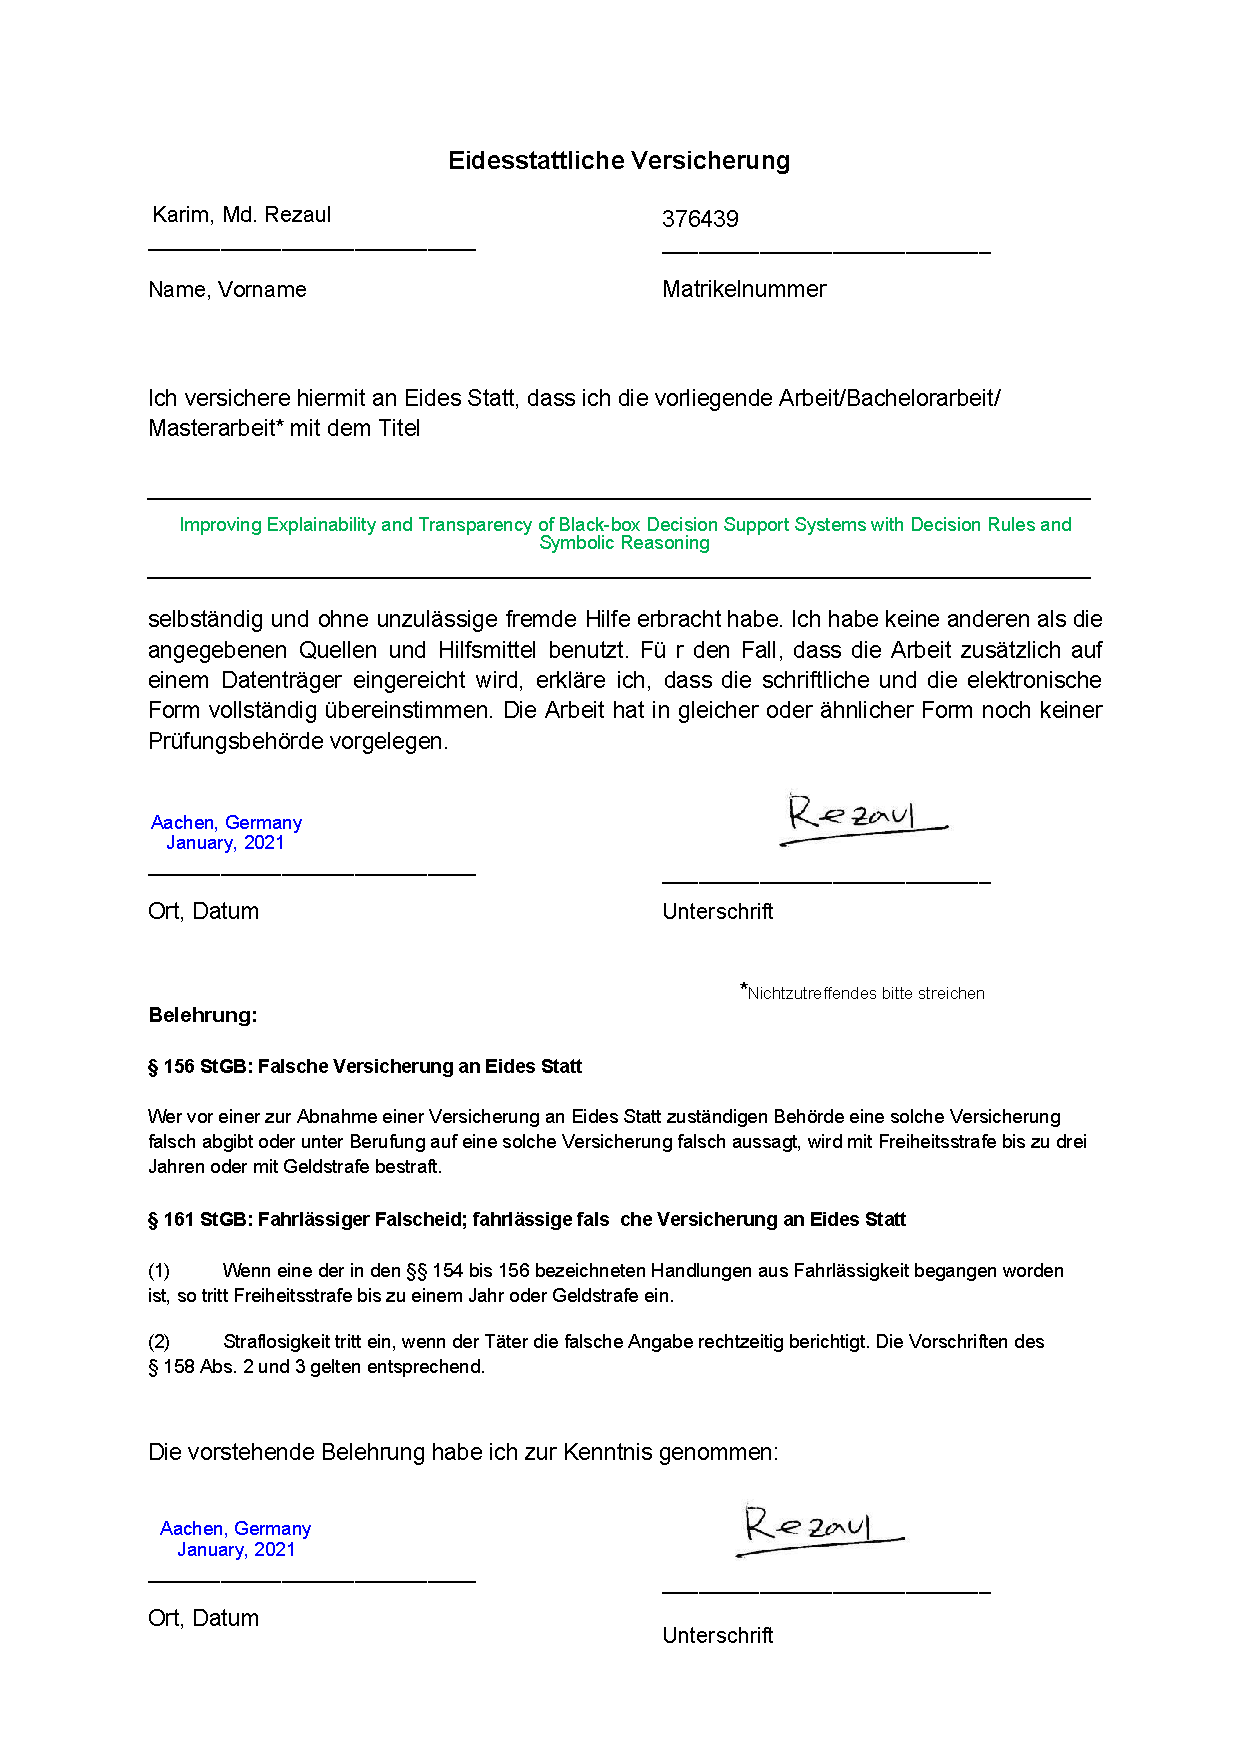
\includepdf[pages=-,pagecommand={},width=\textwidth]{Oathstatement_v3.pdf}

% delete the two declaration sentences in thesis.sty if not applicable. 

\preface
\addcontentsline{toc}{chapter}{Abstract}

\begin{abstract}
    %\centerline{\textit{``Towards Explainable Cancer Prognosis and Prediction Based on Neuro-symbolic
    %Learning and Reasoning''}}
    %\centerline{Md. Rezaul Karim}
    \small{
        \textbf{Background:} deep learning based on neural networks~(DNN) has shown tremendous success in automated decision-making in domains like industrial and chemical engineering, computer vision, healthcare, financial institutions, etc. However, due to  nested non-linear and complex structures, DNN architectures are mostly opaque and perceived as `black box' methods. 
        %without providing enough insights. 
        `Black-box' models not only suffer from a lack of transparency, but also cannot reason about underlying decisions. Such opaqueness raises numerous legal, ethical, and practical concerns. AI-based systems have already been utilized in critical domain like healthcare for automated diagnoses, treatment, and prognosis in a clinical setting. 
        %, e.g. aiming to model the progression and treatment of cancerous conditions. 
        However, if we cannot see how a clinical decision is made, we cannot know what impact it will create on a patient. %, because the day when such AI-guided systems will make life decisions for humans is not very far ahead. 
        %AI-based techniques have been utilized in numerous scenarios, including automated diagnoses and treatment in clinical settings\cite{karimBIB2019}. 
        For example, cancer is one of the deadliest diseases caused by abnormal behaviours of genes that control cell division and growth. As the importance of genetic knowledge in cancer treatment is increasingly addressed, several projects have emerged, producing large-scale omics data. Appropriate diagnoses depend on accurate prediction of cancer types. Therefore, it is crucial to analyze genomics data and clinical outcomes before recommending necessary treatments. Acquiring deep insights of omics data, can provide profound insights to reveal genetic predispositions of cancer before it grows. %Besides, treatment can be focused on preventive measures.  %Eventually, . %Analyzing such data can provide profound insights to reveal genetic predispositions of cancer before it grows. 
        Further, `right to explanation' of GDPR that enforces `algorithmic transparency', gives patients the right to know why and how a diagnosis decision is made. 
        %In this case, interpretability attained with neuro-symbolic reasoning can provide insights into the reasons. % why a given cancer case is of a specific type. 
        %can help in finding more suitable treatments, cures, or drug repositioning. 
        
        \vspace{1mm}
        \textbf{Motivations}: 
        %one of the main differences between ML and symbolic reasoning~(SR) is where the learning happens: a learning algorithm learns rules to establish correlations between inputs and outputs, but rules are generated through human intervention in SR. 
        to build an explainable decision support system~(DSS), humans must learn the rules by which two phenomena relate before embedding those relationships into a static and hard-coded program.
        %A hard-coded rule is a preconception. 
        While a DNN architecture is trained on an assumption on how it should learn rather than what conclusion it should reach, a more effective way is choosing developing a system to learn flexibly and produce accurate decisions. In this case, explicit representation of domain knowledge and data provenance through the layers of a DNN can pave the path to an explainable DSS and improve the transparency and interpretability based on human-understandable decision rules and SR.  
        %generate human-understandable explanations and ensure fairness 
        %by mitigating biases.
        %, where human-understandable decision rules and SR can help improve the transparency and interpretability, generate human-understandable explanations and ensure fairness by mitigating biases. 
        This thesis aims to: i) improve algorithmic transparency and explainability of a `black-box' DSS for cancer diagnosis, ii) discovery and disseminating knowledge of molecular mechanisms of carcinogenesis. 
        
        \vspace{1mm}
        
        \textbf{Methods:} several unimodal and multimodal neural network architectures are first trained on genomics data %and clinical outcome 
        and learn high-level abstract features. Neural ensemble method, 
        %which is more effective than structures solely based on a single model
        is then employed to get the most stable model from multiple model snapshots. To improve algorithmic transparency and interpretability, different probing techniques~(e.g., class activation maps and layer-wise relevance propagation) were employed. To improve adversarial robustness, adversarial training was performed considering different  attacks scenarios.
        Model surrogation strategy is then employed to  generate the explanations in terms of decision rules, focusing both local and global interpretability. %to adversaries and behaves as intended in real-life scenario, a is necessary
        As a part of the SR, a domain-specific knowledge graph~(KG) is developed by integrating knowledge and facts about cancer from external sources. %, which provides the foundation of our semantic layer. 
        A semantic reasoner is then used to learn the hierarchical relations from the KG and to provides the reasoning of diagnosis decision. %, a semantic reasoner is used. %
        %by minimizing prediction biases. 
        Finally, decision rules are updated by combining reasoning and predictions to make the clinical diagnosis more trustworthy. % by the CDSS. %Finally, we assess the explainability and fairness of the overall approach. 
        
        \vspace{1mm}
        
        \textbf{Results:} quantitative and qualitative analyses show that our approach exhibits not only high confidence at predicting the cancer types correctly giving an average precision of 96.25\%, but also provides human-interpretable explanations of the predictions by exposing top genes and cancer-specific driver genes.} 
        %Nevertheless, findings are validated through pathway analysis and annotations provided by the TumorPortal. 
        %We hope our approach will be a useful contribution, particularly towards the development of AI-assisted applications and an acceleration of their adoption in the clinical practice.} 
\end{abstract}
\clearpage
\addcontentsline{toc}{chapter}{Deutsche Zusammenfassung}

\begin{abstract}
%\centerline{\textit{``Towards Explainable Cancer Prognosis and Prediction Based on Neuro-symbolic
%Learning and Reasoning''}}
%\centerline{Md. Rezaul Karim}
\small{
    \textbf{Hintergrund}: Deep Learning auf der Grundlage neuronaler Netze~(DNN) hat sich bei der automatisierten Entscheidungsfindung in zahlreichen Bereichen als äußerst erfolgreich erwiesen. Aufgrund der verschachtelten, nichtlinearen und komplexen Struktur sind DNN-Architekturen jedoch meist undurchsichtig und werden daher als ``Black-Box''-Methoden angesehen. Sie weisen nicht nur einen Mangel an Transparenz auf, sondern können auch zugrunde liegende Entscheidungen nicht begründen. Eine solche Undurchsichtigkeit wirft zahlreiche rechtliche, ethische und praktische Bedenken auf. KI-basierte Systeme wurden bereits in zahlreichen Bereichen wie der automatisierten Diagnose, und Behandlung im klinischen Umfeld eingesetzt. Wenn es uns jedoch nicht möglich ist zu erklären, wie eine klinische Entscheidung zustande kommt, können wir auch die Auswirkungen auf einen Patienten nicht schlecht abschätzen. Und der Tag, an dem solche KI-gesteuerten Systeme Lebensentscheidungen für den Menschen treffen werden, ist nicht sehr weit voraus. Krebs ist eine der weltweit tödlichsten Krankheiten. Sie wird durch abnormales Verhalten von Genen verursacht, welche die Zellteilung und das Zellwachstum kontrollieren. Da eine Krebsdiagnose von der genauen Vorhersage eines Krebstyps abhängt, ist eine genaue Analyse von Genomdaten und anderer klinischer Ergebnisse entscheidend, bevor eine Behandlung empfohlen werden. Die Analyse solcher Daten kann tiefgreifende Erkenntnisse über genetische Prädispositionen liefern und helfen den Krebs möglichst frühzeitig zu erkennen. Darüber hinaus besteht laut DSGVO ein ``Recht auf Erklärung'', welches die ``algorithmische Transparenz'' durchsetzt - das Recht des Patienten zu wissen warum und wie eine Entscheidung durch ein Entscheidungsunterstützungssystem~(DSS) getroffen wird. In diesem Fall, kann das Verfahren der neurosymbolischen Schlussfolgerung~(NSR) entsprechende Einblicke in die Entscheidungsgründe ermöglichen. 
    
    \vspace{1mm}
    \textbf{Motivations}: Einer der wichtigsten Unterschiede zwischen Maschinellem Lernen~(ML) und SR ist die Art und Weise der Lernens: Ein Lernalgorithmus lernt Regeln, um Korrelationen zwischen Eingangs- und Ausgangswerten herzustellen, bei SR hingegen werden die Regeln durch menschliche Eingaben erzeugt. Um ein erklärbares KI~(XAI)-System zu entwickeln, müssen die Beziehungen zwischen Phänomenen zunächst von Menschen in Form von Regeln beschrieben werden. Dann können diese Beziehungen in ein statisches und fest kodiertes Programm eingebettet werden. Die vom Menschen definierten Regel bilden dabei bestehende Expertenmeinungen ab. DNN-Architekturen befolgen hingegen ausschließlich Annahmen darüber, wie sie lernen sollten, und nicht darüber, zu welcher Schlussfolgerung sie gelangen sollen. Eine effektive Möglichkeit besteht darin die Annahmen so zu wählen, dass sie es dem System ermöglichen, möglichst flexibel zu lernen und genaue Entscheidungen über ihre Eingaben zu treffen. In diesem Fall kann die explizite Darstellung von Domänenwissen und Datenprovenienz durch die Schichten eines DNN den Weg zu XAI ebnen, bei dem Interpretierbarkeit, Entscheidungsregeln und SR eingesetzt werden, um menschlich verständliche Erklärungen zu erzeugen. Zugleich werden Verzerrungseffekte minimiert und die Fairness der Ergebnisse gesteigert. Diese Dissertation zielt auf folgendes ab: i) die Verbesserung der Erklärbarkeit, Fairness und Robustheit eines DSS durch den Einsatz von NSR und Entscheidungsregeln, ii) die Entdeckung und Verbreitung von Wissen über molekulare Mechanismen von Krebsgenenomen. 
    
    \vspace{1mm}
    
    \textbf{Methodik}: Wir trainieren verschiedene unimodale und multimodale DNN-Architekturen anhand von Genomdaten und klinischen Ergebnissen, um abstrakte Merkmale auf einer grobgranularen Ebene zu erlernen. Die Methode des neuronalen Ensembles ist effektiver als Methoden, die nur auf einem einzigen Modell basieren und werden angewandt um ein möglichst stabiles Modell zu erzeugen. Anschließend identifizieren wir Krebs-typische Schlüsselgene, indem wir klassenspezifische Regionen mit Hilfe von Class Activation Maps (Grad-CAM++) und Layer-wise Relevance Propagation (LRP) hervorheben. Darüber hinaus erzeugen wir auf Basis zuvor definierter Entscheidungsregel, entsprechende Erläuterungen für jede Entscheidung, wobei wir sowohl lokale als auch auf die globale Interpretierbarkeit einbeziehen. Um die Robustheit zu verbessern, stellen wir zudem verschiedene Arten von Angriffen auf die Modelle vor. Als Teil des SR haben wir durch Integration von Wissen und Fakten über Krebs aus externen Quellen, einen domänen-spezifischen Wissensgraphen (KG) geschaffen, der die semantische Schicht des Systems bildet. Der Reasoner charakterisiert und lernt hierarchische Beziehungen aus dem KG, und liefert Erklärungen für Vorhersagen durch die Minimierung von Vorhersageverzerrungen. Schließlich erzeugen wir faire Entscheidungsregeln, indem wir Begründungen und Vorhersagen kombinieren, um eine vertrauenswürdige die klinische Diagnose zu erzeugen.
    
    \vspace{1mm}
    
    \textbf{Results:} Ergebnisse: Quantitative und qualitative Analysen zeigen, dass unser Ansatz nicht nur eine hohe Konfidenz für die korrekte Vorhersage von Krebsarten mit einer durchschnittlichen Genauigkeit von 96,25\% aufweist, sondern auch menschlich interpretierbare Erklärungen der Vorhersagen liefert, indem er Spitzengene und Krebs-typische Schlüsselgene offenlegt. Wir hoffen, dass unser Ansatz einen nützlichen wissenschaftlicher Beitrag darstellt und zur schnelleren und sichereren Adaption von KI-unterstützten Anwendungen in der klinischen Praxis beitragen wird. 

}
\end{abstract}
%\clearpage

\addcontentsline{toc}{chapter}{Acknowledgements}

\begin{acknowledgements}
    Alhamdulillah, I'd like to express my profound gratitude to Almighty \textbf{Allah}, for His bounties and blessings to complete this dissertation. Then, I'd like to convey my heartiest thanks to all who were with me during this journey towards achieving my doctoral degree at RWTH Aachen University, Germany. Foremost, I'd like to acknowledge my sincere gratitude to my supervisor Prof. Dr. \textbf{Stefan Decker} for hiring me as a Scientist at Fraunhofer FIT and supervising my Doctoral thesis at the RWTH Aachen University. His insightful comments and encouraging remarks addressed during my each presentation patience and supportive guidance throughout my graduate studies at the university. His kind motivation and profound direction allowed me to explore and learn while maintaining a steady course towards the destination. He introduced me to the research areas and provided me with the proper understanding with his expertise. His suggestions and invaluable advice gave subtle direction to my efforts. In a nutshell, I found him very friendly, cooperative, very open-minded, and approachable. 
    %Believe me, I have never been depressed while I was working at Fraunhofer FIT, Germany. 
    
    \hspace*{5mm} Meanwhile, my heartfelt gratitude and thanks endlessly go to my advisors: Dr. Oya Beyan and Dr. Michael Cochez. The door to their offices was always open for me whenever I ran into any difficulties. They consistently motivated me through their domain expert, guidance, and insights and steered me in the right direction whenever I needed it. To Dr. \textbf{Oya Beyan}, I'm very very grateful to her, and I express my sincere gratitude to her for hiring me as a PhD student in Ireland as well as for making me aware of my current research position at Fraunhofer FIT. %I'm forever indebted to her, as I consider her as my key to Europe. 
    
    \hspace*{5mm} To Dr. \textbf{Michael Cochez}, I found him one of my best research mentors, who always thought and motivated me how to research in a structured way, how to think scientifically, and how to write scientific articles. He was not only a mentor to me, but also a good human being whom I could share my research interests and personal matters without hesitations. To the examiner, Prof. Dr. \textbf{Dietrich Rebholz-Schuhmann}, I'm very grateful and indebted to him too for being one of my best mentors and motivating leaders. He has always inspired me since the beginning of my journey in Ireland as well as in Germany. Overall, I am gratefully indebted to all of the above for their prompt, thorough and timely feedback, corrections, and valuable suggestions on this thesis. To be honest, without their passionate participation and immense knowledge in the research and science, solving complex could not have been impossible.
    
    \hspace*{5mm} Next, I am incredibly grateful indebted to my parents \textbf{Abdur Razzaque} and \textbf{Monoara Begum} for their sacrifice and care throughout my life, especially to my father who had a dream that one day I'll finish my Ph.D., which is why I dedicate my thesis to my father. Nevertheless, I am very grateful to my loving wife \textbf{Saroar Zahan} and my son \textbf{Ahmed Shadman} for their patience, contributions, and sincere accompany here in Germany. Their unconditional love and never-ending support gave me the confidence to utilize my abilities. Their prayer and guidance is the reason for where I stand here today. Besides, I would like to thank all of my family members, including my sister Josna Khatun and my brother Mamtaz Uddin, whose immense love, care, and encouragement always gather inspiration in my work and silent acceptance of my long absence from my home country. 
    
    \hspace*{5mm} I would like to graciously acknowledge the help of my current members of Data Science \& AI Department at Fraunhofer FIT and Chair of Computer Science 5 - Information Systems and Databases at RWTH Aachen University, for providing friendly environment at the working place. First, I would like to express my sincere indebtedness to the head of the department Dr. \textbf{Christoph Lange} and other colleagues, including Till D{\"o}hmen, J{\'o}ao Bosco Jares, Yeliz Ucer, Lars Gleim, and Sascha Welten for their expertise and patient guidance throughout this research work. To \textbf{Till D{\"o}hmen}, I'm very thankful for translating me the English abstract of this thesis into German. 
    
    \hspace*{5mm} Besides, I extend my sincere thanks to IT help-desk of Fraunhofer FIT for providing me access to it's computing infrastructure in which I performed most of the experiment, including data processing, storing, training, and analysis. Additionally, I am grateful for the support and help from Mr. Reinhard Linde, Ms. Leany Maassen, Ms. Romina Reddig, and Ms. Tatiana Liberzon. Mr. Reinhard Linde was always accessible and helped create network and computing infrastructures, which substantially boosted the progress of my works. Furthermore, I am grateful to have access to PanCancerAtlas project from The Cancer Genome Atlas~(TCGA). Nevertheless, writing this thesis is made more accessible by incredible efforts by many open source communities and documentations provided by TensorFlow, Keras, Scikit-learn, Python, Apache Spark, RuleMatrix, Skater, ExplainX, and SHAP community and all those who have contributed to APIs, whose work ultimately brought the machine learning to the masses! 
    
    \hspace*{5mm} Nevertheless, I want to acknowledge the help and care of every member of the Bangladeshi Community in Germany. I can never forget the pleasant moments and memories that I passed with this community during my stay here in Germany, including Mr. Sami Chowdhury and Mr. Mesbah Saber, for their love, support and inspiration in removing my loneliness in this place by providing a family-like environment. Finally, I'd like to graciously acknowledge the help and encouragement that I obtained from my childhood friends and well-wishers, including Naimul, Khairul, Rakib, and Mahidul throughout this research work. \\ \\ %I would like to express my heartfelt thanks to all of them for being with me with immense support and care and to make this work successful.
    \\ \\ \\ 
    \flushright Md. Rezaul Karim, MSc. \\
    Computer Science 5 - Information Systems and Databases\\
    RWTH Aachen University\\ 
    Aachen, Germany \\
    March 2021
\end{acknowledgements}
%%\clearpage

\addcontentsline{toc}{chapter}{Acknowledgements}

\begin{acknowledgements}
    Alhamdulillah, I'd like to express my profound gratitude to Almighty \textbf{Allah}, for His bounties and blessings to complete this dissertation. Then, I'd like to convey my heartiest thanks to all who were with me during this journey towards achieving my doctoral degree at RWTH Aachen University, Germany. Foremost, I'd like to acknowledge my sincere gratitude to my supervisor Prof. Dr. \textbf{Stefan Decker} for hiring me as a Scientist at Fraunhofer FIT and supervising my Doctoral thesis at the RWTH Aachen University. His insightful comments and encouraging remarks addressed during my each presentation patience and supportive guidance throughout my graduate studies at the university. His kind motivation and profound direction allowed me to explore and learn while maintaining a steady course towards the destination. He introduced me to the research areas and provided me with the proper understanding with his expertise. His suggestions and invaluable advice gave subtle direction to my efforts. In a nutshell, I found him very friendly, cooperative, very open-minded, and approachable. 
    %Believe me, I have never been depressed while I was working at Fraunhofer FIT, Germany. 
    
    \hspace*{5mm} Meanwhile, my heartfelt gratitude and thanks endlessly go to my advisors: Dr. Oya Beyan and Dr. Michael Cochez. The door to their offices was always open for me whenever I ran into any difficulties. They consistently motivated me through their domain expert, guidance, and insights and steered me in the right direction whenever I needed it. To Dr. \textbf{Oya Beyan}, I'm very very grateful to her, and I express my sincere gratitude to her for hiring me as a PhD student in Ireland as well as for making me aware of my current research position at Fraunhofer FIT. %I'm forever indebted to her, as I consider her as my key to Europe. 
    
    \hspace*{5mm} To Dr. \textbf{Michael Cochez}, I found him one of my best research mentors, who always thought and motivated me how to research in a structured way, how to think scientifically, and how to write scientific articles. He was not only a mentor to me, but also a good human being whom I could share my research interests and personal matters without hesitations. To the examiner, Prof. Dr. \textbf{Dietrich Rebholz-Schuhmann}, I'm very grateful and indebted to him too for being one of my best mentors and motivating leaders. He has always inspired me since the beginning of my journey in Ireland as well as in Germany. Overall, I am gratefully indebted to all of the above for their prompt, thorough and timely feedback, corrections, and valuable suggestions on this thesis. To be honest, without their passionate participation and immense knowledge in the research and science, solving complex could not have been impossible.
    
    \hspace*{5mm} Next, I am incredibly grateful indebted to my parents \textbf{Abdur Razzaque} and \textbf{Monoara Begum} for their sacrifice and care throughout my life, especially to my father who had a dream that one day I'll finish my Ph.D., which is why I dedicate my thesis to my father. Nevertheless, I am very grateful to my loving wife \textbf{Saroar Zahan} and my son \textbf{Ahmed Shadman} for their patience, contributions, and sincere accompany here in Germany. Their unconditional love and never-ending support gave me the confidence to utilize my abilities. Their prayer and guidance is the reason for where I stand here today. Besides, I would like to thank all of my family members, including my sister Josna Khatun and my brother Mamtaz Uddin, whose immense love, care, and encouragement always gather inspiration in my work and silent acceptance of my long absence from my home country. 
    
    \hspace*{5mm} I would like to graciously acknowledge the help of my current members of Data Science \& AI Department at Fraunhofer FIT and Chair of Computer Science 5 - Information Systems and Databases at RWTH Aachen University, for providing friendly environment at the working place. First, I would like to express my sincere indebtedness to the head of the department Dr. \textbf{Christoph Lange} and other colleagues, including Till D{\"o}hmen, J{\'o}ao Bosco Jares, Yeliz Ucer, Lars Gleim, and Sascha Welten for their expertise and patient guidance throughout this research work. To \textbf{Till D{\"o}hmen}, I'm very thankful for translating me the English abstract of this thesis into German. 
    
    \hspace*{5mm} Besides, I extend my sincere thanks to IT help-desk of Fraunhofer FIT for providing me access to it's computing infrastructure in which I performed most of the experiment, including data processing, storing, training, and analysis. Additionally, I am grateful for the support and help from Mr. Reinhard Linde, Ms. Leany Maassen, Ms. Romina Reddig, and Ms. Tatiana Liberzon. Mr. Reinhard Linde was always accessible and helped create network and computing infrastructures, which substantially boosted the progress of my works. Furthermore, I am grateful to have access to PanCancerAtlas project from The Cancer Genome Atlas~(TCGA). Nevertheless, writing this thesis is made more accessible by incredible efforts by many open source communities and documentations provided by TensorFlow, Keras, Scikit-learn, Python, Apache Spark, RuleMatrix, Skater, ExplainX, and SHAP community and all those who have contributed to APIs, whose work ultimately brought the machine learning to the masses! 
    
    \hspace*{5mm} Nevertheless, I want to acknowledge the help and care of every member of the Bangladeshi Community in Germany. I can never forget the pleasant moments and memories that I passed with this community during my stay here in Germany, including Mr. Sami Chowdhury and Mr. Mesbah Saber, for their love, support and inspiration in removing my loneliness in this place by providing a family-like environment. Finally, I'd like to graciously acknowledge the help and encouragement that I obtained from my childhood friends and well-wishers, including Naimul, Khairul, Rakib, and Mahidul throughout this research work. \\ \\ %I would like to express my heartfelt thanks to all of them for being with me with immense support and care and to make this work successful.
    \\ \\ \\ 
    \flushright Md. Rezaul Karim, MSc. \\
    Computer Science 5 - Information Systems and Databases\\
    RWTH Aachen University\\ 
    Aachen, Germany \\
    March 2021
\end{acknowledgements}
\clearpage
%\clearpage
%\addcontentsline{toc}{chapter}{Acronyms}
\section*{Acronyms}
Acronyms and their full forms used across the chapters in this thesis are listed down: 

\begin{multicols}{2}
\begin{description}[leftmargin=0pt]
\scriptsize{
        %\item [ARI] Adjusted Rand Index
        %\item [ALWMMFC] Autoencoder Loss with Mixture Model for Clusters
        \item [AE] Autoencoder
        \item [AAE] Adversarial Autoencoder
        \item [ACC] Adrenocortical Cancer	
        \item [AEx] Adversarial Examples
    	\item [AUC] Area Under Receiver Operating Characteristic Curves
    	\item [BO] Bayesian Optimization
    	\item [BLCA] Bladder Urothelial Carcinoma
    	\item [BRCA] Breast Invasive Carcinoma
    	%\item[BACH] BreAst Cancer Histology images
    	\item [CNN] Convolutional Neural Network
        %\item[CC] Centroid-based Clustering
        %\item[CC1] Clustering Classification
        %\item [CAH] Clustering Assignment Hardening
        \item [CHOL] Cholangiocarcinoma	
        \item [COAD] Colon Adenocarcinoma
        \item [CESC] Cervical and Endocervical Cancer
        %\item [CDEC] Convolutional Deep Embedded Clustering
        %\item[CCNN] Clustering using CNN
        \item [CAE] Convolutional Autoencoder
        \item [ACC] Clustering Accuracy
        \item [CAM] Class Activation Maps
        \item [CN] Copy Numbers
        \item [CNA] Copy Number Aberration
        \item [CDSS] Clinical Decision Support System
        \item [DLBC] Diffuse Large B-cell Lymphoma	
        %\item[CXR] Chest X-ray
        %\item[CNN] Convolutional Neural Network
        %\item [CLRP] Contrastive Layer-wise Relevance Propagation
        \item [CNV] Copy Number Variations
        \item [CAC] Cyclic Cosine Annealing
        \item [CNS] Copy Number Segment
        \item [DL] Deep Learning
        \item [DLx] Description Logic
        \item [DBN] Deep Belief Networks
        %\item[DEC] Deep Embedded Clustering
        %\item[DCN] Deep Clustering Network
        \item [DR] Dimensionality Reduction
        %\item[DC] Distribution-based Clustering
        %\item[DC1] Density-based Clustering
        %\item[DCC] Deep Continuous Clustering
        %\item[DBC] Discriminatively Boosted Clustering
        \item [DSAE] Denoising Stacked AE
        %\item [DEN] Deep Embedding Network
        %\item[DEPICT] Deep Clustering with CAE embedding
        %\item [DAC] Deep Adaptive Image Clustering 
        \item [DNN] Deep Neural Networks
        \item [DL] Deep Learning 
        \item [DT] Decision Trees
        %\item [DenseNet] Dense Convolutional Network
        \item [DTD] Deep Taylor Decomposition
        \item [EM] Expectation Minimization
        \item [ER] Estrogen Receptor
        \item [ESCA] Esophageal Carcinoma
        %\item [FFNN] Feed-forward Neural Networks
        \item [FCL] Fully-Connected Layer
        \item [FI] Feature Importance
        %\item[FCN] Fully Convolutional Neural Network
        \item [FM] Feature Maps
        \item [FNR] False Negative Rate
        \item [FPR] False Positive Rates
        \item [GE] Gene Expression
        \item [GBM] Glioblastoma Multiforme
        \item [GDC] Genomic Data Commons
        \item [GB] Guided Backpropagation
        \item [GAG] Globally Averaged Gradients 
        \item [GDPR] General Data Protection Regulation
        \item [GV] Genomic Variants
        \item [GAP] Global Averaged Pooling 
        \item [GMM] Gaussian Mixture Model
        \item [GAN] Generative Adversarial Networks
        \item [GLW] Greedy Layer-wise Training
        \item [GBT] Gradient Boosted Trees
        \item [GOFAI] Good Old-Fashioned Artificial Intelligence
        \item [GRC] Genome Reference Consortium
        \item [Grad-CAM] Gradient-guided Class-activation Maps
        \item [HM] Heat Maps
        \item [HNSC] Head and Neck Squamous Cellcarcinoma
        \item [HER2] Human Epidermal Growth Factor Receptor 2
        %\item [HC] Hierarchical Clustering
        %\item[HQ] High Quality
        %\item [HGE] Histogram Equalization
        \item [HDO] Human Disease Ontology
        \item [ICU] Intensive Care Unit
        %\item [IFS] Incremental Feature Selection
        \item [IEx] Isoform Expression
        %\item[IMSAL] Info Maximization and Self-augmentation Loss
        %\item [JULE] Joint Unsupervised Learning of Deep Representation for Images
        \item [KLD] Kullback-Leibler Divergence
        \item [KNN] K-nearest Neighbours 
        \item [KB] Knowledge Base
        \item [KIRC] Kidney Clear Cell-carcinoma
        \item [KICH] Kidney Chromophobe
        \item [KIRP] Kidney Papillary Cell-carcinoma
        \item [KG] Knowledge Graphs
        \item [LAML] Acute Myeloid-leukemia
        %\item [LPL] Locality Preserving Loss 
        %\item [LP+GS] Locality Preserving and Group Sparsity
        %\item[LQ] Low QualitY
        \item [LSTM] Long Short-Term Memory
        \item [LR] Learning Rate
        \item [LGG] Brain Lower-grade Glioma
        \item [LIHC] Liver Hepatocellular Carcinoma
        \item [LUAD] Lung Adenocarcinoma	
        \item [LRP] Layer-wise Relevance Propagation
        \item [LUSC] Lung Squamous Cell-carcinoma
        \item [MESO] Mesothelioma	
        \item [ML] Machine Learning 
        \item [MGI] Mouse Genome Informatics
        \item [MAI] Mean Absolute Impact
        %\item[ML] Machine Learning
        \item [MLP] Multilayer Perceptron
        %\item [MMMC] Max Margin for Mixture Components
        %\item[MQ] Medium Quality
        \item [NMI] Normalized Mutual Information
        \item [NE] Number of Epochs
        \item [NB] Naive Bayes
        \item [NS] Number of Cycles
        \item [NE] Number of Epochs
        \item [NGS] Next Generation Sequencing
        \item [OOD] Out-of-distribution
        \item [OOG] Ontology of Genes and Genomes
        \item [OECC] Outlier Exposure with Confidence Control
        \item [OV] Ovarian Serous Cystadenocarcinoma
        %\item[K-medoids] Partitioning Around Medoids
        \item [PAAD] Pancreatic Adenocarcinoma
        \item [PD] Partial Derivatives
        \item [PCA] Principal Component Analysis
        \item [PCPG] Pheochromocytoma and Paraganglioma
        \item [PCAt] PanCancerAtlas
        \item [PRAD] Prostate Adenocarcinoma
        \item [PM] Permutation Model
        %\item [PMF] Perona-Malik Filter
    	%\item [PM] Prediction Maximization
    	%\item [PPV] Positive Predictive Value
    	\item [POTSF] Proto-oncogenes with Tumor-suppressor Function
    	\item [RBM] Restricted Boltzmann Machines
    	\item [PR] Progesterone Receptor
    	\item [ROC] Receiver Operating Characteristic
    	%\item [ResNet] Residual Network 
    	\item [ReLU] Rectified Linear Unit
    	\item [READ] Rectum Adenocarcinoma
    	\item [RNN] Recurrent Neural Networks
    	\item [RS] Relevance Score
        \item [RL] Representation Learning
        \item [RL1] Reconstruction Loss
        \item [RF] Random Forest
        \item [SW] Semantic Web
        \item [SARC] Sarcoma
        \item [SKCM] Skin Cutaneous Melanoma
        \item [SVM] Support Vector Machines
    	\item [SM] Saliency Maps
    	%\item [SCF] Self-consistent Field
    	\item [SHAP] SHapley Additive exPlanations
    	%\item [SGD] Stochastic Gradient Descent
    	\item [SBRL] Scalable Bayesian Rule List
    	%\item [SCPA] Softmax Class Posterior Averaging
        %\item [SOM] Self-Organizing Maps
        \item [SNV] Single Nucleotide Variation
        \item [SNP] Single Nucleotide Polymorphism
        \item [SGD] Stochastic Gradient Descent
    	\item [SGLRP] Softmax-gradient LRP
    	\item [STAD] Stomach Adenocarcinoma
    	\item [TCGA] The Cancer Genome Atlas
    	\item [TL] Transfer Learning
    	\item [TGCT] Testicular Germcell Tumor
    	\item [TPR] True Positive Rate
    	\item [TF] Transcription Factors
    	\item [THCA] Thyroid Carcinoma
    	\item [THYM] Thymoma
    	\item [UCS] Uterine Carcinosarcoma
        %\item [UDA] Unsupervised Data Augmentation
        \item [UCEC] Uterine Corpus Endometrioid Carcinoma
        \item [UVM] Uveal Melanoma
        \item [VAE] Variational Autoencoder
        %\item [WCSS] Within-cluster Sum of Squares
        \item [XAI] eXplainable Artificial Intelligence
        }
\end{description}
\end{multicols}
%\clearpage
%\addcontentsline{toc}{chapter}{Acronyms}
%\section*{Acronyms}
\begin{dedication}
    Dedicated to my father!
\end{dedication} 

\body
\chapter{Introduction}
\label{chapter:introduction}
\textit{"An approximate answer to the right problem is worth a good deal more than an exact answer to an approximate problem"}- John Tukey

\section{Chapter Overview}
Decision support system~(DSS) is an information system that supports business or organizational decision-making activities\footnote{\url{https://en.wikipedia.org/wiki/Decision_support_system}}. A typical DSS is takes a set of input, e.g., factors, numbers, and characteristics to analyze and transforms data from which DSS `decisions' are generated. Finally, results generated by the DSS based on user criteria, which is often annotated or validated with User knowledge and expertise. In other words, a DSS is  often a computerized program assists which sifts through and analyzes massive amounts of data, compiling comprehensive information that can be used to solve problems and in decision-making. On the other hand, a DSS that can perform selected cognitive decision-making functions based on artificial intelligence~(AI) or intelligent agents technologies called intelligent DSS. 

\hspace*{3.5mm} Owing to outstanding performance across domains such as computer vision, natural language processing, multimedia analytics, and business analytics, AI-guided DSS could eventually be applied to various automated decision-making process. In an AI-guided or intelligent DSS, a set of learning algorithms are embedded to perform cognitive decision-making in which machine learning~(ML) often act as one of the most common forms of AI. ML is about using a set of statistical and mathematical algorithms to perform tasks such as concept learning, predictive modeling, clustering, and mining useful patterns can be performed. The most complex forms of ML involve deep learning~(DL), or deep neural network~(DNN) models with many levels of features or variables that predict outcomes that help take meaningful decision. However, DNN models are perceived mostly as `black box' methods because of their not well-understood internal functioning. Besides, they cannot reason their underlying decisions, leaving them incapable of aiding transparent and trustworthy decisions. Consequently, we call such DSS a `black box' model. 

\hspace*{3.5mm} Throughout this thesis we aim to improve the transparency and explainability of such black-box DSSs. This chapter provides a general introduction to this dissertation, provides the motivation for this research, list down the hypotheses and research questions, and outlines the structure of this thesis. 
%In particular, \cref{chapter:preli} discusses the reason of cancer and outlines it's severity.
\Cref{motivations}, outlines the specific motivations underpinning this research. \Cref{problem_challenges}, discusses the research problems and points out several challenges concerning the research problems. \Cref{goals} discusses the goal of this thesis including a workflow diagram. \Cref{hypotheses} presents the hypotheses and research questions derived from the previously reported work on cancer prediction and diagnosis. \Cref{contributions} lists the contributions of this dissertations. \Cref{structure} outlines the organisation and structure of the thesis.

%\section{Introduction}

\section{Motivations}\label{motivations}
Intelligent DSSs are often ML or DL-based DSS, where a ML or DL algorithm is employed to improve the learning experience such that it becomes automatic by reducing the level of human interaction as much as possible. In many domains, applying ML and getting higher prediction accuracy is not enough. Eventhough some ML models maybe better at predicting, detecting, and processing patterns better than humans, they cannot reason or explain. In fact, in many cases, the goal is not only predicting something with a high-level of confidence, rather better understanding. 

\hspace*{3.5mm} Moreover, real-life data contain heterogeneity, high variability, and high dimensionality, which imposes significant challenges to existing ML methods stimulating the development of DL-based DSS. Nevertheless, our real world experience is multimodal~\cite{mmsurvey}, e.g., while watching a movie, we not only observe the movie itself but the acting, background music, action, background scenario, and landscapes, etc. To tackle these, approaches based on DL work better with such high dimensional data, recent studies focused on using different DNN architectures based on autoencoders, convolutional neural network~(CNN), and recurrent neural network~(RNN). Although many existing approaches based on DNN have shown tremendous success in solving such problems, DNN models are perceived mostly as `black box' methods because of their not well-understood internal functioning. Subsequently, they cannot reason their underlying decisions, leaving them incapable of providing transparent and trustworthy decisions. 

\hspace*{3.5mm} Furthermore, since the opaqueness raises numerous legal, ethical, and practical concerns, transparency and accountability in AI-based systems have to ensure. From practical point of view, if we cannot see how the predictions were made, we cannot know what impact will happen on human lives, as the day when such AI-guided machines take life decisions for humans is not very far ahead. The General Data Protection Regulation~(GDPR)~\cite{kaminski2019right}, approved by the European Parliament in 2018, suggests that individuals should be able to obtain explanations of the decisions made from their data by automated processing, and to challenge the decision. The article 22 states that individuals ``have the right not to be subject to a decision based solely on automated processing" and ``whenever human subjects have their lives significantly impacted by an automatic decision-making machine, the human subject has the right to know why the decision is made", i.e., `right to explanation'. In other words, GDPR prohibits the use of ML for automated decisions unless a clear explanation of the logic used to make each decision is well explained. 

\hspace*{3.5mm} To understand the negative impacts of a `black-box'-based DSS, let's assume a simple example of a man named John, who is a typical bank customer. Suppose John~(like most customers today) applies for a credit (loan) from a bank. whenever you interact with a company oftentimes data about you ends up getting sent into some kind of model. In this case, if you're in a financial institution, often these models are trying to predict 
things that you care about in terms of outcomes. So in this case, predicting whether John has any repayment problems. So here, a chance of 55 percent leads to the bank denying his loan. So in this case, there's a standard thing that happens thousands of times every day around the world, and it leads to questions from John, obviously, like, why did you deny my loan? If you have a good manager, you should also ask the same question, right? Why are we making these really business-critical decisions? But unfortunately, sometimes for the data scientist who built the model was all about accuracy for them. They would not have good answers when they're trying to explain the reason.

\begin{figure*}[h]
	\centering
	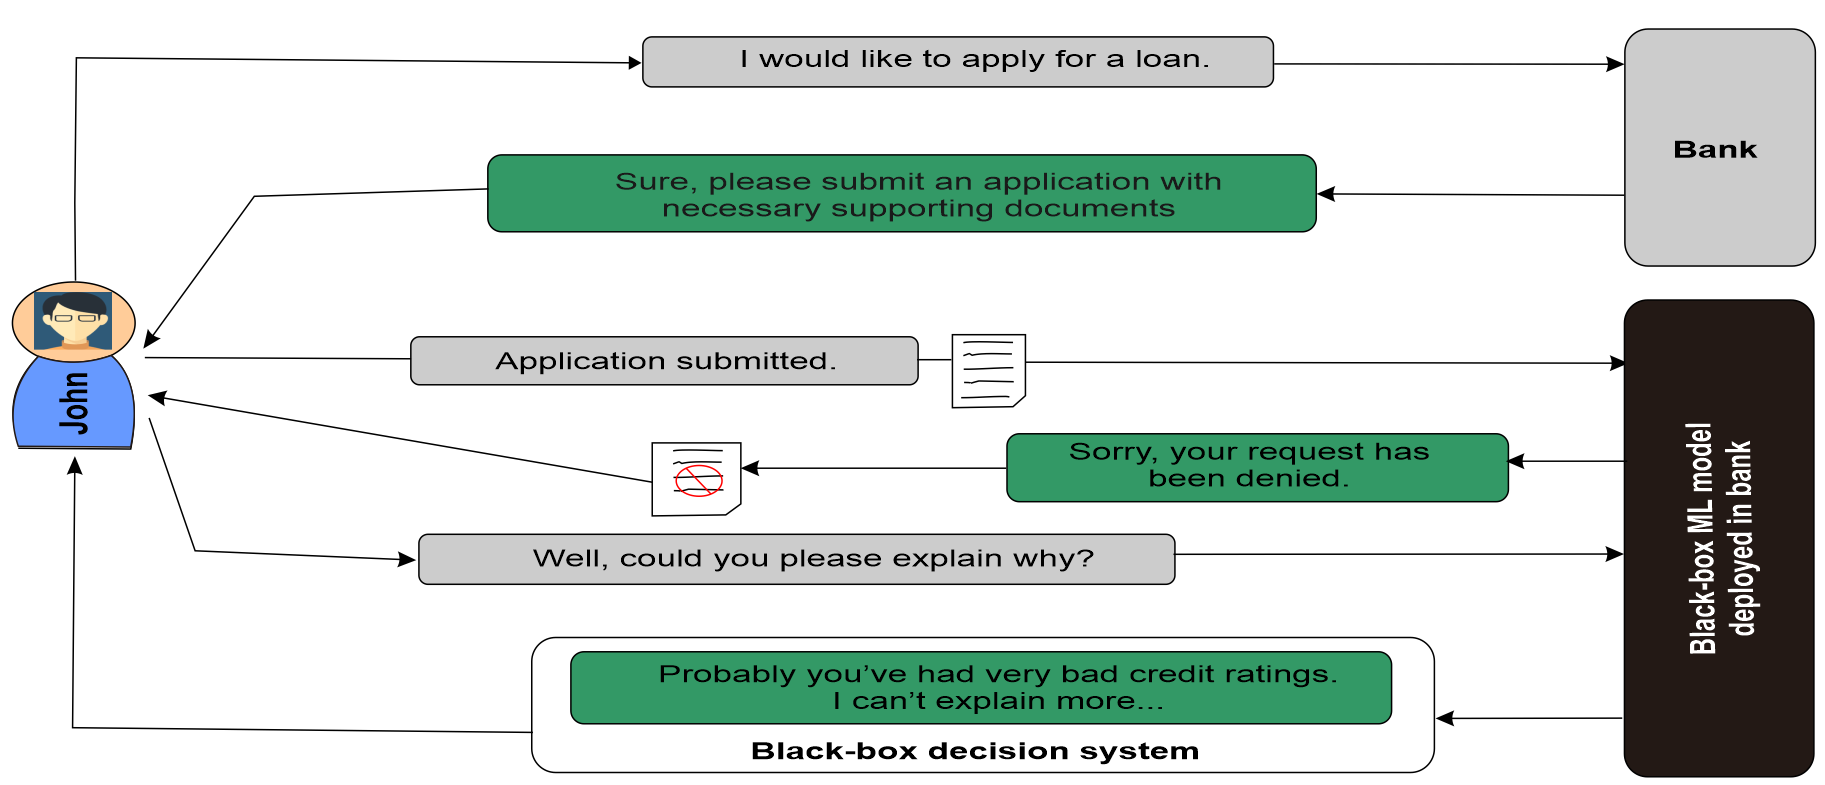
\includegraphics[width=0.9\linewidth,height=80mm]{images/loan.png}
	\caption{Problems of model opacity}
    \label{fig:model_bbm}
    \vspace{-2mm}
\end{figure*}

\hspace*{3.5mm} So why does this happen? Well, it happens often because many times you run into a trade-off between a complex model, where because you have a very, very large potentially complicated dataset, you can take advantage of the flexibility of these complex models, and get a lot of accuracy. But that can lead to a lack of interpretability. In contrast, some simple models can be interpretable in the right contexts, but if there are too restrictive, they'll lead to a lack of accuracy.
Okay? This is what often leads people to run into this in practice, particularly in finance. So if you have interpretability or accuracy and you can link choose one, that's a painful trade-off. For the bank, it's particularly painful because accuracy directly corresponds to money for them, because accuracy will correspond to default rates for the loans. But interpretability is really important. Because if you're interpretable, you have happy customers.

\hspace*{3.5mm} There's also really important legality concerns as GDPR and other things. So there are strong drivers on both sides of this trade-off for the many companies. Now, one thing you can do is try and make simple models better, right? So that you can improve their ability to retain the interpretability and also move towards accuracy. That's a great approach. We're actually going to focus on the other one though, which is basically, taking what's already considered very complex models and trying to extract interpretability from them. Okay? So if you do that though and you just look at a complex model by itself, it could be very complicated in the mapping, and trying to explain an entire mapping space could just be hopelessly complex. So instead what we're going to do is focus on explaining individual predictions one at a time, because those involve, perhaps, just a small piece of the overall complexity of the model. 

\hspace*{3.5mm} So I don't have to describe how a model behaves in all circumstances in order to tell John what was going on with his loan, I just need to tell him what was going on that affected him. So if we do that, one way to go about it is to say, "Let's start with a simple model and see what this means, be really specific and concrete." So here's a a linear model. Why do we consider these things interpretable? Often, it's because they have this giant summation sitting in the middle of the model, right? So we have a bunch of terms coming in. These are things about John, let's say, these input attributes, and a bunch of terms come together and they just get summed up and sent to you as some output. Okay? So we think of these as interpretable because we can look at that and see a bunch of things coming together additively, and what's coming into the summation can be viewed as a credit that's attributed to each input feature. 

\hspace*{3.5mm} In contrast, if we look at a complex model, say a neural net or a random forest, maybe gradient boosted decision trees, things like this. Often, there's so much going on in there that there's not a nice term that we can just surface and say, "This is how the model's going." So what we're going to talk about is, how we can explain an individual prediction in a way very similar to how a linear model works, where again we're going to have a summation sitting inside there. But now, instead of having just terms that are straight from the definition of the model, we're going to have to come up with our own definition of a credit attributed to each feature. Okay? So this Phi function is going to be indexed by the feature and it depends both on the model and the current input. Okay? So we're essentially replacing the input to a summation that you would get in a linear model with something that represents the importance of that feature in the complicated model. One such AI-guided clinical decision support system~(CDSS) is used in healthcare is increasingly been applied and adopted. For example, AI-based systems have already been deployed in diagnosis, treatment recommendations, patient engagement, and administrative activities. There are many instances, where AI already outperforming healthcare tasks in automated diagnoses and treatment in clinical setting, e.g., outperforming radiologists at spotting malignant tumours, model the progression and treatment of cancerous conditions. Besides, AI is guiding researchers in how to construct cohorts for costly clinical trials~\cite{davenport2019potential}. 

\hspace*{3.5mm} A more concrete example of using AI-guided systems in healthcare is carcinogenesis. In cancer genomics, not only recommending accurate diagnosis and subsequent treatment, but also knowing the biological mechanisms is important, e.g., oncogenes. Cancer has been characterized as a heterogeneous disease consisting of many different types and subtypes. Consequently, it is one of the deadliest diseases caused by abnormal behaviors of genes alterations and abnormal behaviors of genes that control cell division and cell growth. The change in the structure of occurring genetic aberrations, such as somatic mutations, copy numbers~(CN), profiles, and different epigenetic alterations are unique for each type of cancer~\cite{82Tomczak,13cancerdef,19Cruz}. As a result, gene expression~(GE) can be disrupted by cell division, environmental effects, or genetically inherited from parents. Changes in GEs sometimes change the production of different proteins, affecting normal cell behavior. These damaged cells start reproducing more rapidly than usual and gradually increase in the affected area by forming a tumor. 

\hspace*{3.5mm} Intermittently, such tumors turn into a type of cancer~\cite{zuo2019identification,24Podolsky}. This is one of the utmost reasons cancer incidences are gradually increasing and become the second leading cause of death worldwide. More than 200 types of cancer have been identified in which each type can be characterized with different molecular profiles requiring unique therapeutic strategies~\cite{82Tomczak}. According to a statistic from the National Cancer Institute\footnote{\url{https://www.cancer.gov/about-cancer/understanding/statistics}}, there were around 14.1 million cancer cases in 2012 in which as many as 8.8 million people died of five leading cancers of lung, liver, colorectal, stomach, and breast~\cite{stat}. In 2018, an estimated 17.35 million new cases of cancer have been diagnosed in the United States in which 609,640 people died. The number of new cancer cases per year is expected to rise to 23.6 million by 2030, which is anticipated to increase further by 70\% by 2035~\cite{71Torre}. 

\hspace*{3.5mm} On the other hand, cancer is not only a lethal disease but tremendously complex to diagnose and treat. However, discovery of important biomarkers is a significant step towards understanding the molecular mechanisms of carcinogenesis and prognosis of certain cancer type. Knowing the important biomarkers enables recommending accurate drug repositioning. However, for recommending any diagnosis, multi-omics data and clinical information need to be processed for understanding the genetic and epigenetic causes before recommending appropriate treatment. Such data include gene/miRNA expression, DNA methylation, copy number variation~(CNVs), mutations, bioimaging~(e.g., histology and radiological images), and reports)~\cite{22Ding, 23Zheng}.  

\begin{figure*}[h]
	\centering
	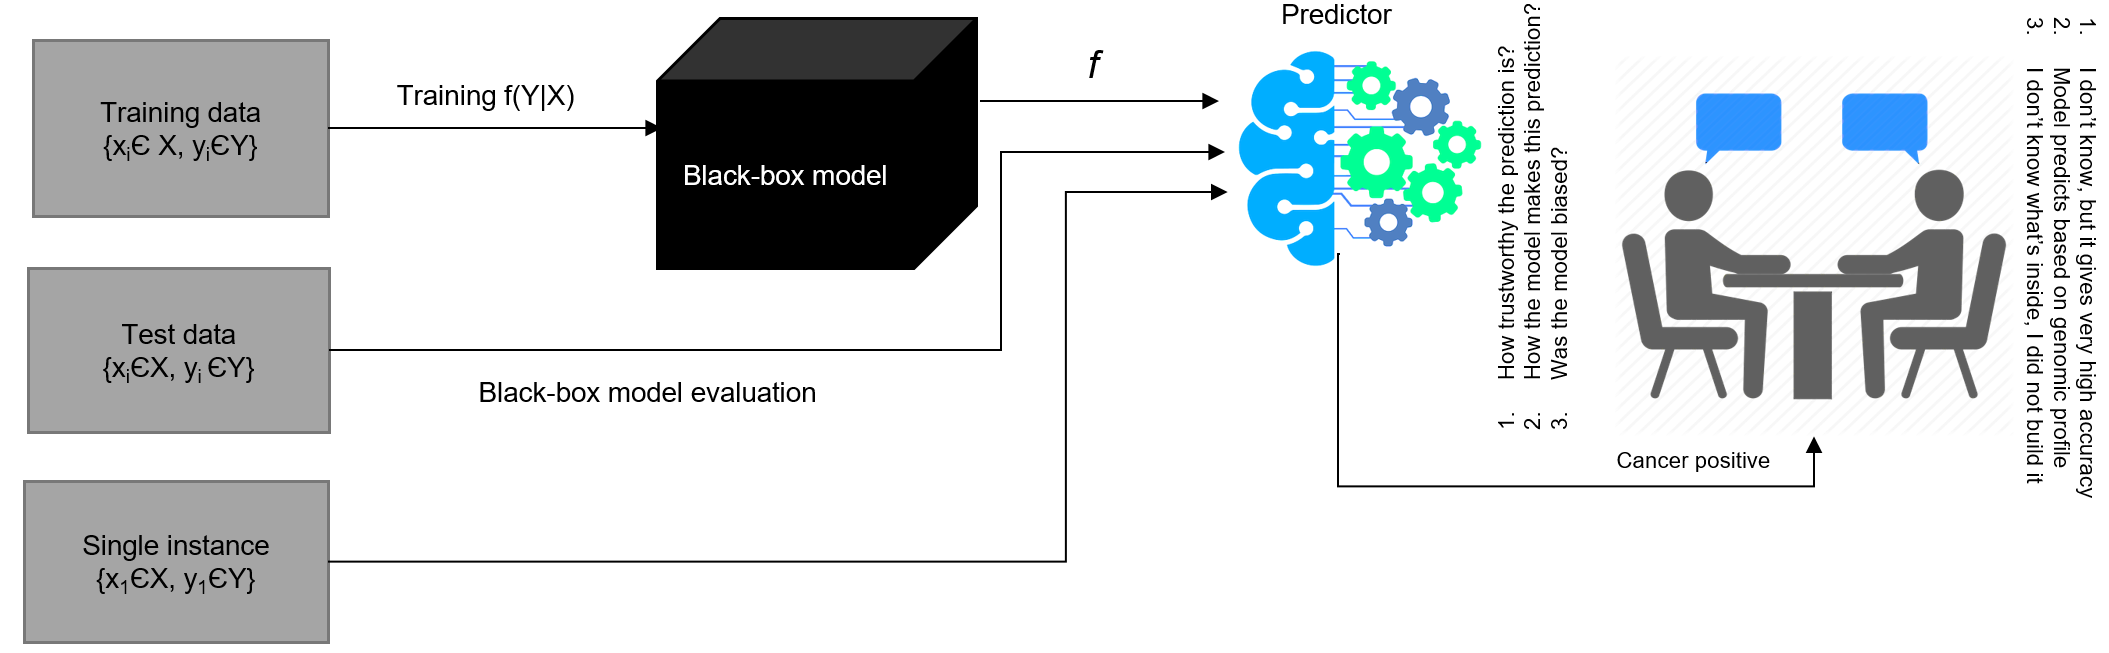
\includegraphics[width=0.9\linewidth]{images/bbm.png}
	\caption{Problems of model opacity}
    \label{fig:model_bbm}
    \vspace{-2mm}
\end{figure*}

\hspace*{3.5mm} Further, by acquiring insights from omics data, treatment can be focused on preventive measures. As the importance of genetic knowledge in cancer treatment is increasingly addressed~\cite{15Wu}, several projects have emerged. In particular, the next generation sequencing~(NGS) is playing a key role in therapeutic decision making for the cancer prognosis and treatment~\cite{jha2017towards}. The NGS technologies are producing a massive amount of sequencing datasets too. For example, the cancer genome atlas (TCGA)~\cite{tomczak2015cancer} is best known for omics data and is a collection of bio-molecules inside living things such as genomics, metabolomics, and proteomics. However, omics data are generated from multiplatform and heterogeneous sources, which needs to be analyzed to make clinical decisions, where both multimodality and heterogeneity impose great challenges to bioinformatics tools and computational algorithms~\cite{karimACCESS2019,karimBIB2019}. 

\hspace*{3.5mm} However, diagnosis and prognosis, especially for specific cancer types is not straightforward. In fact, the diagnosis of a breast cancer patient depends on several distinct molecular subtypes, e.g., multiple factors are involved~(e.g., in cancer diagnosis, estrogen receptor~(ER), progesterone receptor~(PGR), and human epidermal growth factor receptor 2~(HER2/neu statuses for breast cancer), providing AI-based diagnoses might not be accurate solely based on CNVs. This requires using multimodal features based on DNA methylation, gene expression, miRNA expression, and CNVs data by creating a multiplatform network to support each data type, where the DSS based on genomics data from different cohorts will be more reliable. Subsequently, an early diagnosis of cancer~(e.g., classifying cancer patients into high or low risk groups) have become essential in cancer research, as it can facilitate the subsequent clinical management of patients~\cite{kourou2015machine}.  

\section{Thesis Goal} \label{thesis_goal}
%Although these models have shown tremendous success in exhibiting high confidence, they are mostly perceived as `black box' methods because of a lack of understanding of their internal functioning. 
Current cancer typing methods focused on employing ML approaches and using mixed data types to handle the high dimensionality and heterogeneity. However, except for the linear and tree-based models, DNN models are perceived mostly as `black box' methods because of their not well-understood internal functioning. Often, we don't fully understand how and which factors tend a model to make a prediction right and why it will fail in certain cases. These are serious drawbacks. However, knowing the cancer type and most relevant biomarkers is the prerequisite for an oncologist to recommend more accurate treatments and drug repositioning. 
Although, it is understandable that not every prediction made by an ML algorithm needs to be explained, in many cases, ML models itself have to be interpretable enough such that it can provide the reasoning, such that it also allows healthcare experts to make reasonable and data-driven decisions to provide personalized diagnosis or treatment decisions that can lead to higher quality of service in healthcare~\cite{stiglic2020interpretability}.
Higher interpretability of an ML model means easier comprehension and explanation of future predictions for end-users. 

\hspace*{3.5mm} Besides, since many AI systems are being deployed to make critical decisions in sensitive environments~\cite{stiglic2020interpretability}, it is important to ensure that the decisions made by the system is not only accurate and trustworthy, but do not reflect discriminatory behavior toward certain groups or populations~\cite{mehrabi2019survey}. Based on these motivations, developing an explainable clinical decision support system to improve the transparency and trustworthiness for real-life problems, e.g., to aid the cancer diagnosis is the main goal of this thesis, such that the CDSS should be able generate accurate and trustworthy predictions in a transparent way, identifies misclassified instances, uses the existing knowledge from the knowledge base~(KB), and produces new knowledge, answers, and provides human-interpretable explanations about the prediction made. 

\begin{figure*}[h]
	\centering
	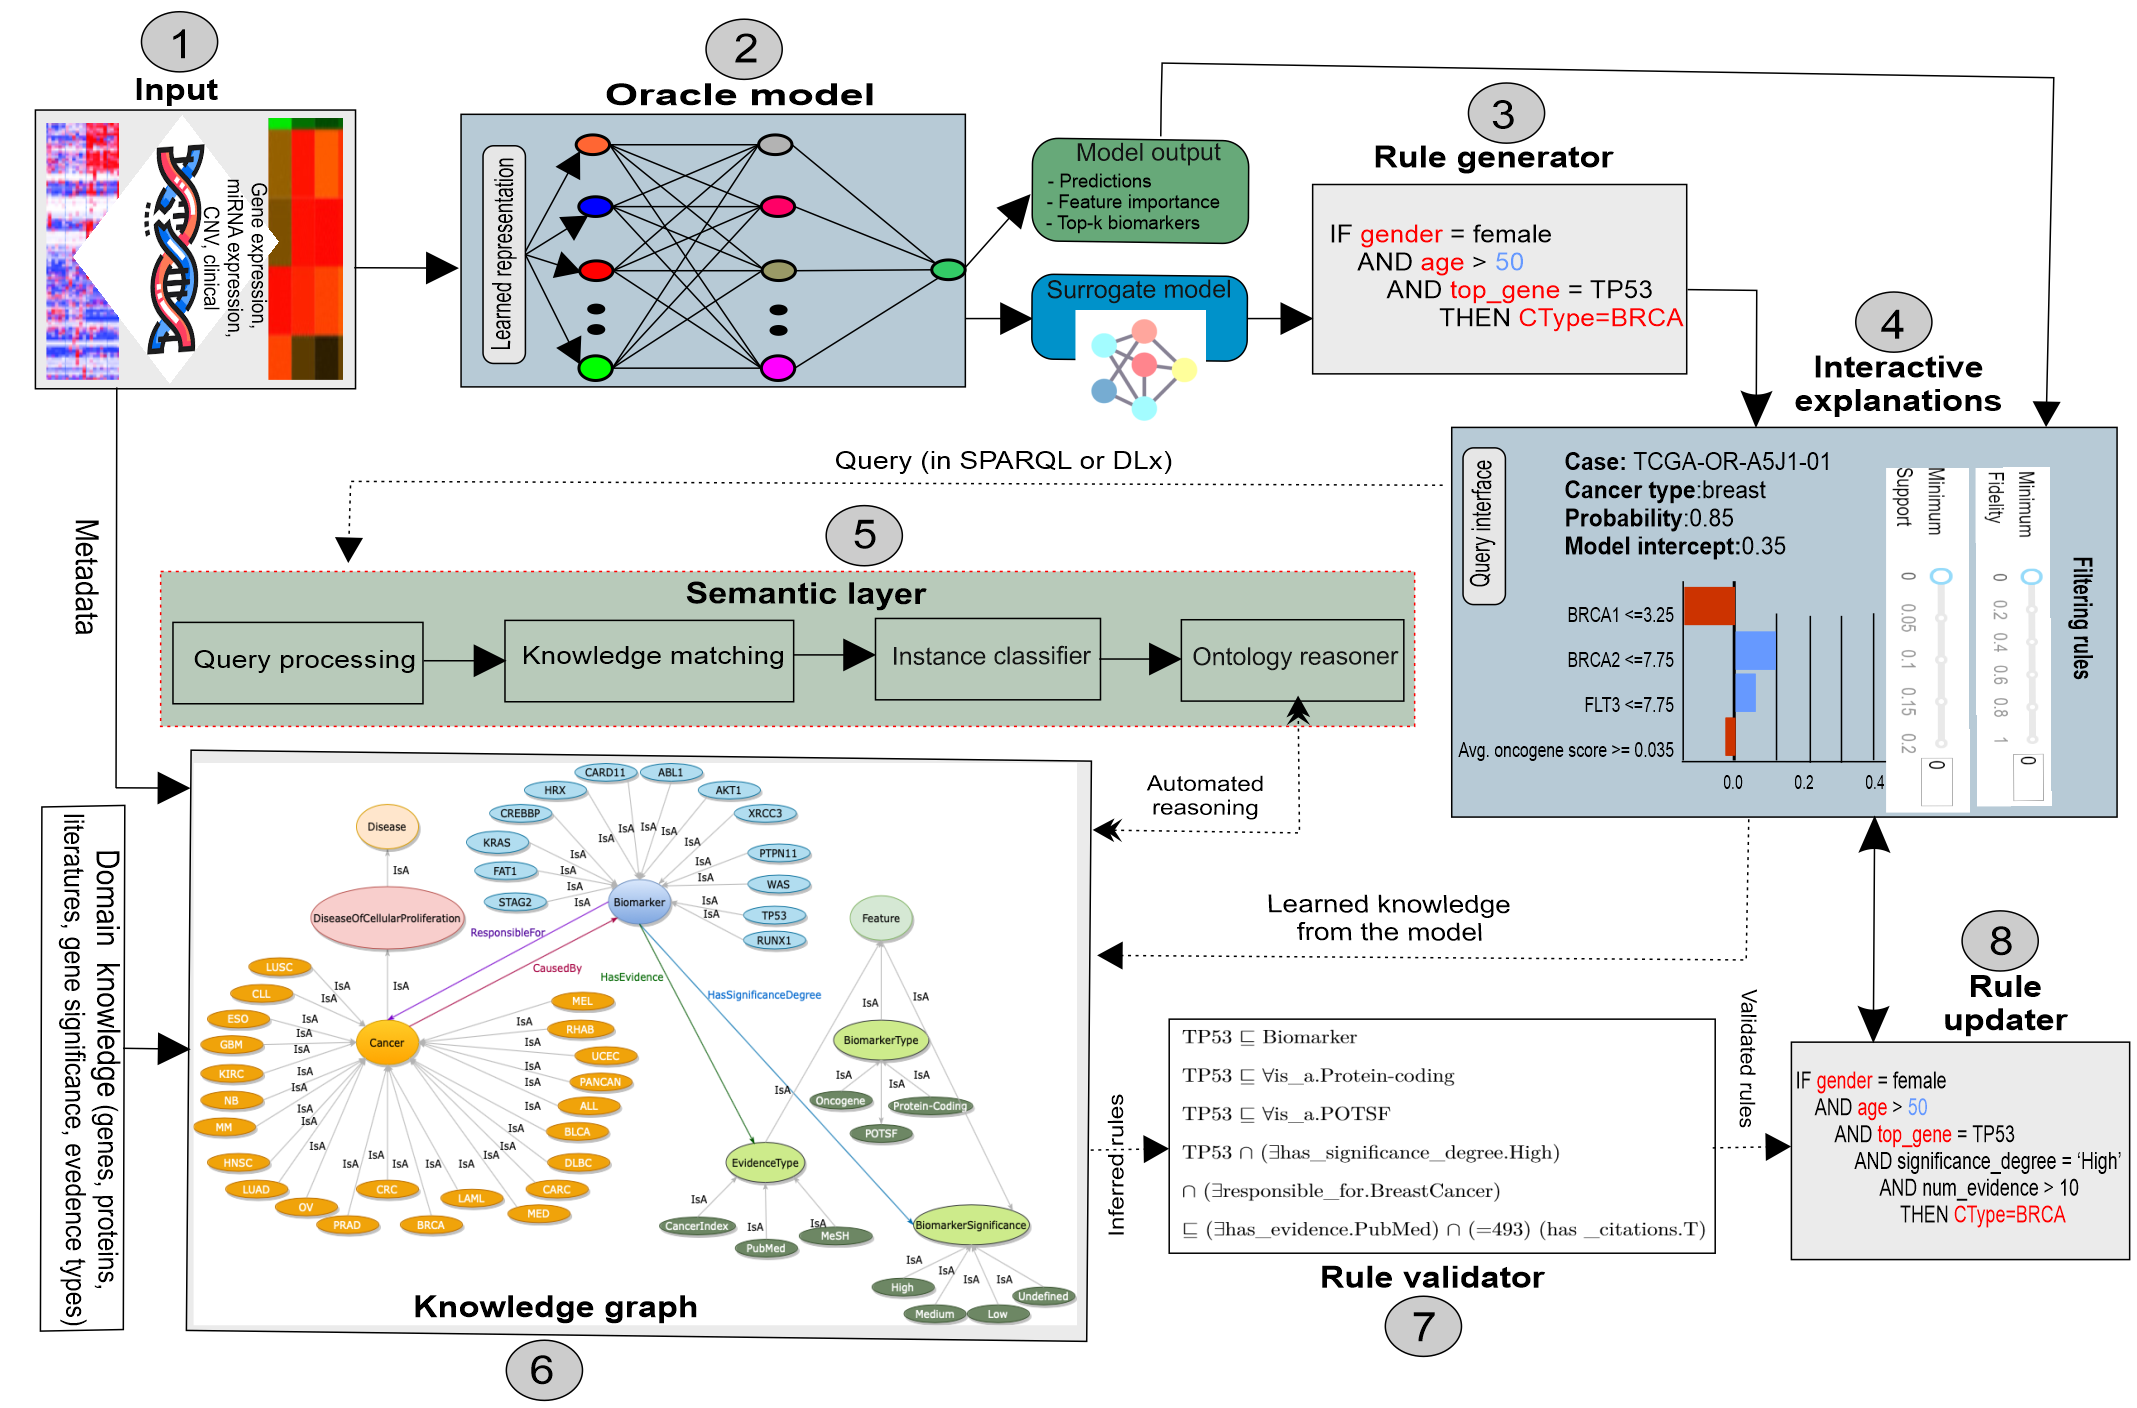
\includegraphics[width=\textwidth,height=95mm]{images/reasoning_wf.png}	
    \caption{Workflow for improving the explainability and transparency of a clinical DSS}
	\label{fig:wf_overall_approach}
\end{figure*}

\section{Problem Statement} \label{problem_challenges}
Human-interpretable explanations can: i) help identify cancer types, ii) learn similarities between cancer patients, iii) patients themselves can see what types of decision are made and why. Eventually, these features will help doctors recommend better treatments, e.g., allow for drug repositioning. To do so, we model cancer typing method as a prediction task, but in a multi-class classification setting: from a given genomic dataset $D$ about $n$ patients, $X$ = ${\mathbf{\{x_1,x_2,..., x_n}}\}$, where $x_k \in \mathbb{R}^{d}$. We consider classifying an individual $x_i$ into a specific cancer type based on his or her genomic profile. However, instead of classifying samples directly using their original representation $X$, we first transform the data with a nonlinear mapping $F_{\theta}: X \rightarrow Z$, where $\theta$ are learnable parameters and $Z \in \mathbb{R}^{K}$ is the learned or embedded feature space, where $K \ll D$. 

\hspace*{3.5mm} To parametrize $F_{\theta}$, we employ neural network-based representation learning~(e.g., autoencoders) due to their function approximation properties and feature learning capabilities~\cite{xie2016unsupervised} from genomic data. Based on the embedding $Z$, classifier $F$ maps an input $x$ to an output $F: \mathbb{R}^{d} \mapsto y$. When we assume $F$ has a parametric form, we write $F_{\theta}$, where ${L}(F(x), y)$ denotes the loss function used to train $F$ on $D$ of input-output pairs $(x,y)$. However, since the decision made by the model cannot be traced back to the inputs, nor is it clear why the outputs are transformed the way they are, we treat $F$ a `black-box' model. 

%\section{Thesis Goal} \label{goals}
%Since an efficient ML model maybe better at predicting, detecting, and processing patterns then a human being, they intrinsically it cannot reason. Nevertheless, it is important to take fairness issues into consideration while developing such an explainable artificial intelligence~(XAI) system, 

\iffalse
\begin{figure*}[h]
	\centering
		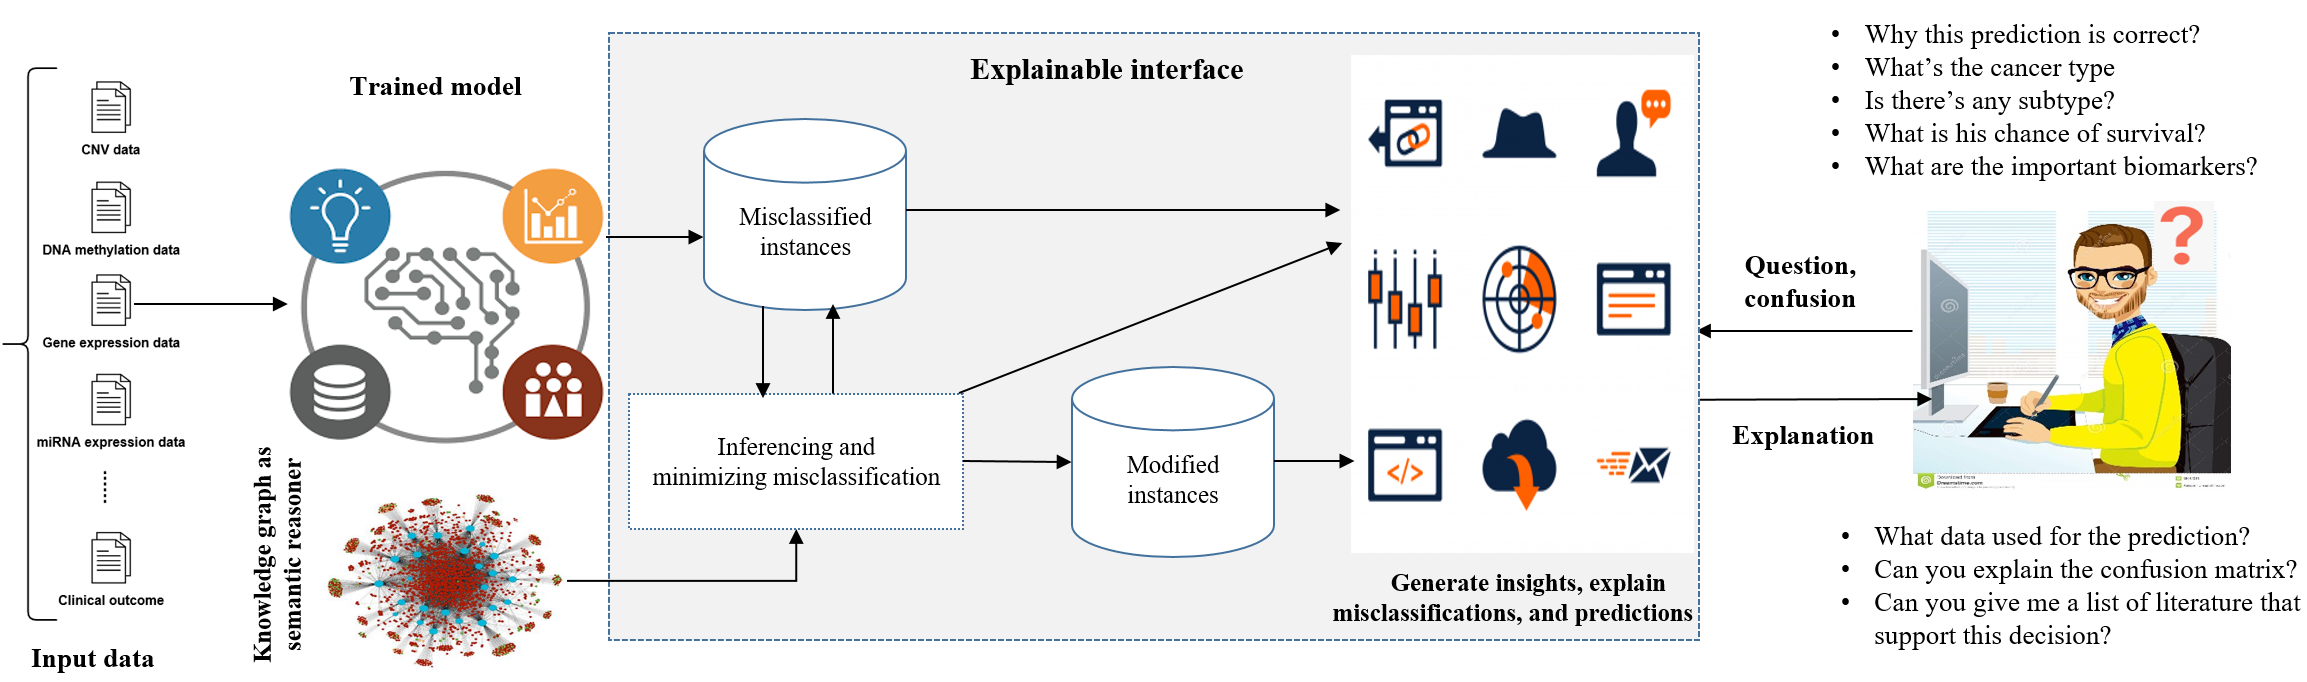
\includegraphics[width=\linewidth,height=60mm]{images/wf2.png}
		\caption{Workflow of the proposed model for explainable predictions of cancer}
        \label{fig:chapter_1_wf}
\end{figure*}
\fi 
%\subsection{Scope of the thesis}
%In the present study, a novel OA quantification solution based on multimodality integration is applied to overcome the limitations of the state-of-the-art approaches by effectively getting rid of the negative influences stemming from modality-forming principles. In terms of their complementary and application range, following a series of preprocessing methods, including contrast enhancement, noise elimination, and multi-slice integration, aiming at the same patient, radiographs and MRIs from axial, sagittal as well as coronal plane are respectively classified by their extracted features in the detected ROIs. Given supplying reliability and objectivity of the grading process, class-discriminating attention maps are generated by Class Activation Maps (CAM), prior to the averaging ensemble of models with the same modality and multimodality. 

\section{Hypotheses and Research Questions} \label{hypotheses}
To disseminating biological knowledge about carcinogenics through the proposed XAI system, the author suggests the following hypotheses to solve several research questions.  
\subsection{Research questions}
To develop an explainable model and to improve the fairness and transparency of a clinical decision support system~(CDSS), this thesis attempts to solve the following research questions: 

\vspace{-2mm}
\begin{itemize}[noitemsep]
    \item \textbf{RQ1}: \textit{How can multimodal data be more effective than unimodal data to provide accurate decision?} As mentioned earlier, multiple factors are involved in cancer diagnosis, genomics data such as GE, miRNA expression, copy numbers, and clinical outcome have to use together to build a more efficient model to accurately predict the outcome of a diagnosis decision.  
    \item \textbf{RQ2}: \textit{How to identify relevant features or factors for a certain decision?} Identification of important biomarkers that contributed most~(i.e., some of the features have a higher impact than others), which facilitates the identification and validation of the presence of cancer and also help determine its stage, subtype, and whether they will respond to therapy. Cancer biomarkers are also of potential therapeutic targets and a key in sequence-specific gene silencing therapy against cancer by selectively silencing aberrantly activated oncogenes.  
    \item \textbf{RQ3}: \textit{How to provide human-understandable interpretations of the decisions using decision rules?} Decision rules are more effective at providing intuitive explanations. Using a set of rules, it is possible to explain a decision directly to humans with the ability to look up the reason for a decision. 
    %\textbf{${RQ}_5$}: How to generate human-interpretable decision rules to provide transparent cancer diagnosis? \\
    \item \textbf{RQ4}: H\textit{ow to disseminate and validate embedded domain knowledge in the model?} An explainable ML model can not only provide predictions, but also insights such as gave top biomarkers, gene correlations, biomarkers types, etc. These help understand the mechanisms of carcinogenesis by further validating the diagnosis with expert and domain knowledge. 
    \item \textbf{RQ5}: \textit{How to score a `black-box' model on transparency?} Knowing the answer to this question will enable us why did the model behave in a certain way? 
\end{itemize}
\vspace{-2mm}

\subsection{Hypothesis}
We hypothesize that our approach based on DL and ML baselines with the explanation capability can be more effective at learning hierarchical features. We embed both local and global interpretability logic and interpretability layer to make ``black-box" model interpretable, which we hope to explain a data point $x$ using an explanation function $g$. We employ several local and global explanation methods to reason the predictions made by the model and mitigate the diagnosis decision biases. Local interpretability refers to an explanation giving reasoning why the model $F$ has predicted $F(x)$ for a fixed point $x$, during inferencing. Since providing human-level interpretability by ``zooming in" individual predictions makes the explanation more trustworthy~\cite{ribeiro2018anchors}, we answer the following questions based on local explanation methods: 

%\vspace{-2mm}
\begin{itemize}[noitemsep]
    \item Which feature $x \in X$ was most important for a certain prediction with $F$? 
    \item Which training data point $z \in \mathbb{R}^{K}$ was most important to $F(x)$? 
    \item What minimal change is necessary to input $x$ to change the output $F(x)$~(e.g., sensitivity analysis)? 
\end{itemize}
%\vspace{-2mm}

\hspace*{3.5mm} On the other hand, global interpretability signifies the overall transparency of the model inside a model on an abstract level. We answer following questions based on global explanation methods: 

%\vspace{-2mm}
\begin{itemize}[noitemsep]
    \item Which features in $X$ were most important across predictions for $F$? 
    \item Which training data points $z \in \mathbb{R}^{K}$ were most important to $F(X)$? 
    \item What minimal change is necessary to input $X$ to change the output $F(X)$~(e.g., sensitivity analysis)? 
\end{itemize}
%\vspace{-2mm}

\hspace*{3.5mm} We train and evaluate several deep architectures with interpretability capabilities, generate heat maps~(HM) for the classes and compute the feature importance in terms of mean absolute impact~(MAI) to identify important biomarkers, provide interpretations of the predictions, and decision visualization to make the cancer diagnosis transparent. Further, we validated our findings through functional analysis to make sure the selected genes are biologically trustworthy for the corresponding tumor types. Further, we will validate our findings based on the annotations provided by the TumorPortal to ensure the consistency and accuracy. In the same line, the symbolic reasoning over neural networks~(aka. neuro-symbolic reasoning), which can fuse the ability of DNNs models can be used to learn probabilistic correlations from scratch alongside abstract and higher-order concepts in order to provide human-interpretable explanations, and error corrections. \Cref{fig:wf_overall_approach} depicts the workflow of the proposed model for explainable predictions of cancer. This thesis make the following hypotheses, which will lead towards potential solutions to the research questions mentioned above in case they are confirmed:

%\vspace{-2mm}
\begin{itemize}[noitemsep]
    %\textbf{$H_2$}: neural representation learning can be more effective for learning high-level abstract features against data sparsity. \\
    \item \textbf{H1}: Multimodal genomics data and clinical outcomes can be used to train a multimodal neural network architecture to provide more accurate clinical diagnostic decision. 
    \item \textbf{H2}: A neural ensemble method, combining several deep architectures, can be more effective than structures solely based on a single model by reducing the generalization error. 
    \item \textbf{H3}: Since genomics data are high dimensional, embedding them into 2D raw images can help locate significant~(i.e, most and least) biomarkers. 
    \item \textbf{H4}: Interpretability provides insights on why/how a certain clinical diagnostic decision is recommended, highlighting significant~(i.e, most and least) biomarkers for further validation. 
    \item \textbf{H5}: Ontological reasoning can help characterize errors w.r.t their hierarchical relations from the KB that helps in decision reasoning.
    %A reasoner then can interact with the learning algorithm as a semantic referee. \\
    \item \textbf{H6}: Fair decision rules can be deduced by combining predictions and reasoning. 
\end{itemize}
%\vspace{-2mm}

\hspace*{3.5mm} To reach the goal, we solve the above research questions, which are driven by the hypotheses. \Cref{fig:wf_overall_approach} outlines the workflow of the overall approach. 

\section{Key Contributions} \label{contributions}
The main contributions of this thesis can be summarized as follows:

\begin{itemize}[noitemsep]
    \item We prepared a rich labelled multimodal genomics data for cancer type prediction that can be used to develop an efficient XCDSS\footnote{Explainable clinical decision support system}.  
    \item We trained several robust neural network models in which different interpretable~(e.g., feature attribution methods) and explainable logic~(e.g., Grad-CAM, LRP) are embedded. These approach enhance the capability of the learning algorithm to identify most significant biomarkers and provide class-specific explanations giving the top-k and common genes across cancer types. 
    \item We performed adversarial training to make the explainable model robust against different types of attacks, such as content moderation and out-of-distribution attacks. 
    \item A novel method of generating decision rules for cancer diagnosis by combing model prediction, biomarkers, and reasoning based on neuro-symbolic reasoning. 
    \item We took both proactive and reactive measures to make the diagnosis decision fair by mitigating different types of bias. 
    \item Comprehensive evaluations of our approach with detailed analyses of outcomes and comparisons with state-of-the-art. 
\end{itemize}

\hspace*{3.5mm} These contributions were reflected into 3 directions: i) peer-reviewed scientific publications, ii) public talks and presentations, iii) open source contributions~(i.e., implementations of some approaches presented). %A number of peer-reviewed publications were produced while conducting the work in this thesis. They are mentioned below, and a note is made to their relevant chapters. 

\subsection{Relevant publications}
The above contributions to science were reflected in a number of peer-reviewed publications. It is to be noted that some of the publications help build the foundations of this thesis. In addition, notes are made to their relevant chapters: 

\begin{enumerate}
	\item {Alokkumar Jha, Yasar Khan, Muntazir Mehdi, \textbf{Md. Rezaul Karim}, Qaiser Mehmood, Achille Zappa, Dietrich Rebholz-Schuhmann, and Ratnesh Sahay, ``Discovering Biomarker and Pathway for Gynecological Cancers", \emph{Journal of Biomedical Semantics}, 8(1), September 2017, DOI: 10.1186/s13326-017-0146-9.} 
	
	\textbf{Abstract}: In this paper, we present an approach to link and query different sequencing datasets such as TCGA, COSMIC, REACTOME, KEGG, and GO to indicate risks of different cancer types. We analyse the tissue expression of genes, CNV, somatic mutation, and promoter methylation to identify associated pathways and find novel biomarkers. 
	
	\textbf{Relevance}: this publication helps provide basic understanding of carcinogenics and different types of genomics data needed to be analyse towards biomarker discovery in \cref{chapter:introduction} and \cref{chapter:preli}. In fact, while working on the paper, I get acquainted with cancer genomic data for the first time. Subsequently, I contributed in the generation of 5* linked data that were lately integrated to form a large-scale knowledge graphs. 
	
	\textbf{Link}:~\url{https://jbiomedsem.biomedcentral.com/articles/10.1186/s13326-017-0146-9}
	
	\item \textbf{Md. Rezaul Karim}, Stefan Decker, Oya Beyan, ``Cancer Risk and Type Prediction Based on Copy NumberVariations with LSTM and Deep Belief Networks", \emph{Proc. of Artificial Intelligence International Conference (A2IC'2018)}, November 21-23, Barcelona, Spain. 
	
	\textbf{Abstract}: In this paper, we apply DL methods to identify cancer and tumor types using CNVs extracted from cancer genomics data from TCGA. We identify and extract CNVs based on long short-term memory~(LSTM) and deep belief networks~(DBN). These were trained using two different representations of CNVs: based on oncogenes and all human genes. Due to lack of sufficient amount of labeled data, we pre-trained the DBN in an unsupervised way then the supervised fine-tuning was carried out using both feed-forward and LSTM networks. 
	
	\textbf{Relevance}: this publication was one of the first attempts to apply DL in cancer types prediction, which motivates us employing more advanced DNN architectures in chapter \ref{chapter:uni_modality}, \ref{chapter:multiodality}, \ref{chapter:xai}, and \ref{chapter:robustness}.
	
	\textbf{Link}:~\url{https://www.premc.org/doc/A2IC2018/A2IC2018_Book_Of_Abstracts.pdf}
	
	\textbf{GitHub}:~\url{https://github.com/rezacsedu/Cancer-Risk-Type-Prediction-CNV-LSTM-DBN}
	
	\item \textbf{Md. Rezaul Karim}, Oya Beyan, Achille Zappa, Ivan G. Costa, Dietrich Rebholz-Schuhmann, Michael Cochez, and Stefan Decker, ``Deep Learning-based Clustering Approaches for Bioinformatics", \emph{Briefings in Bioinformatics}, 02 February, 2020.
	
	\textbf{Abstract}: In this paper, we review state-of-the-art DL-based approaches for cluster analysis that are based on representation learning. We also discussed why and how the representation learning based on different autoencoder architectures are more effective at clustering high dimensional datasets than classic clustering algorithms~(e.g., K-means), covering bioimaging, GE, and biomedical texts. 
	
	\textbf{Relevance}: this publication forms the foundations of representation learning based on variational, LSTM, and convolutional autoencoders used in chapter \ref{chapter:multiodality}, \ref{chapter:xai}, and \ref{chapter:robustness}.

	\textbf{Link}:~\url{https://academic.oup.com/bib/advance-article/doi/10.1093/bib/bbz170/5721075}
	
	\textbf{GitHub}:~\url{https://github.com/rezacsedu/DL_Clustering_Bioinformatics}
	
	\item \textbf{Md. Rezaul Karim}, Michael Cochez, Oya Beyan, Dietrich-Rebholz Schuhmann, and Stefan Decker, ``Convolutional Embedded Networks for Population Scale Clustering and Bio-ancestry Inferencing", \emph{IEEE/ACM Transactions on Computational Biology and Bioinformatics}, 2020.
	
	\textbf{Abstract}: in this paper, we proposed convolutional embedded networks~(CEN) in which we combine two DNN architectures called convolutional embedded clustering~(CEC) and convolutional autoencoder~(CAE) classifier for clustering individuals and predicting geographic ethnicity, respectively, based on genetic variants~(GVs). We employed CAE-based representation learning on GVs from the `1000 genomes' and `Simons genome diversity' projects. This publication forms the foundations of representation learning based on CAE used in \cref{chapter:uni_modality} and \cref{chapter:xai}.

	\textbf{GitHub}:~\url{https://github.com/rezacsedu/Recurrent-Deep-Embedding-Networks}
	
	\item \textbf{Md. Rezaul Karim}, Stefan Decker, Oya Beyan, ``Drug-Drug Interaction Prediction Based on Knowledge Graph Embeddings and Convolutional-LSTM Network", \emph{In Proc. of ACM International Conference on Bioinformatics, Computational Biology, and Health-informatics~(ACM-BCB)}, Niagara Falls, New York, USA, September 7-10, 2019.
	
	\textbf{Abstract}: In this paper, we propose a new approach for predicting drug-drug interactions~(DDI) with Convolutional-LSTM network trained on multiple data sources. For this task we use drug features from DrugBank, PharmGKB, and KEGG drugs, which are integrated using Knowledge Graphs~(KGs). Our evaluations against several baseline models outperforms state-of-the-art approaches. 
	
	\textbf{Relevance}: this publication further motivates us employing Conv-LSTM network in \cref{chapter:uni_modality}.
	
	\textbf{Link}:~\url{https://dl.acm.org/doi/10.1145/3307339.3342161}

	\textbf{GitHub}:~\url{https://github.com/rezacsedu/DDI-prediction-KG-embeddings-Conv-LSTM}
	
	\item \textbf{Md. Rezaul Karim}, Ashiqur Rahman, Stefan Decker, and Oya Beyan, ``A snapshot neural ensemble method for cancer type prediction based on copy number variations", accepted for publication in \emph{Neural Computing and Applications}, 30 November 2019. 
	
	\textbf{Abstract}: in this paper, we used CNVs data covering different cancer types from The Cancer Genome Atlas~(TCGA).We construct two sparse representations of CNVs based on oncogenes and protein-coding genes. Then we train Conv-LSTM and convolutional autoencoder~(CAE) networks using both representations and create snapshots models. While the Conv-LSTM can capture locally and globally important features, CAE can utilize unsupervised pre-training to initialize the weights in the subsequent convolutional layers against the sparsity. Model averaging ensemble~(MAE) is then applied to combine the snapshot models in order to make a single prediction. 
	
	\textbf{Relevance}: this publication further forms the foundation of applying snapshot neural ensemble technique in chapters \ref{chapter:uni_modality} and \ref{chapter:xai}.
	
	\textbf{Link}:~\url{	https://link.springer.com/article/10.1007/s00521-019-04616-9}
	
	\textbf{GitHub}:~\url{https://github.com/rezacsedu/Cancer-type-prediction-CNV_LSTM-CAE} 
	
	\item \textbf{Md. Rezaul Karim}, Stefan Decker, Oya Beyan, ``Prognostically Relevant Subtypes and Survival Prediction for Breast Cancer Based on Multimodal Genomics Data", \emph{IEEE Access}, September 2019.
	
	\textbf{Abstract}: In this paper, we propose a new approach to analyze genomics data from TCGA to classify breast cancer patients based on their subtypes and survival rates. We used DNA methylation, GE, and miRNA expression data by creating a multiplatform network called multimodal autoencoders~(MAE) classifier to support each data type.
	
	\textbf{Relevance}: this publication further forms the foundation of applying MAE technique in \cref{chapter:xai}.
	
	\textbf{Link}:~\url{https://ieeexplore.ieee.org/document/8839793}
	
	\textbf{GitHub}:~\url{https://github.com/rezacsedu/MultimodalAE-BreastCancer}
	
	\item \textbf{Md. Rezaul Karim}, Michael Cochez, Oya Beyan, Stefan Decker, and Christoph Lange-Bever, ``OncoNetExplainer: Explainable Predictions of Cancer Types Based on Gene Expression Data", \emph{In proc. of IEEE International Concerence on Bioinformatics and Bioengineering~(BIBE 2019)}.
	
	\textbf{Abstract}: In this paper, we propose a new approach called \emph{OncoNetExplainer} to make explainable predictions of cancer types based on GE data on which we trained CNN and VGG16 networks using GradCAM++. We generate class-specific heat maps to identify significant biomarkers and computed feature importance to rank top genes across all the cancer types. Further, we identified top genes, and cancer-specific driver genes using gradient boosted trees and SHapley Additive exPlanations~(SHAP). Findings were validated with the annotations provided by the TumorPortal. 
	
	\textbf{Relevance}: this publication further forms the foundation of applying MAE technique in \cref{chapter:xai}.
	
	\textbf{Link}:~\url{https://ieeexplore.ieee.org/document/8941872}

	\textbf{GitHub}:~\url{https://github.com/rezacsedu/XAI_Cancer_Pred}
\end{enumerate}

%The articles in this dissertation are all related to knowledge evolution. The Venn diagram in fig. 7 depicts the relation between the research topics introduced in the previous chapter and the papers. Note that it does not necessarily depict the relations between the research topics in a broader sense1.  Each of the following sections describes the contributions to a topic from that figure. 

\subsection{Public conference talks}
The candidate participated several conferences as the part of the journey of this thesis: 
\begin{enumerate}[noitemsep]
    \item 10$^{th}$ International Semantic Web Applications \& Tools for Healthcare and Life Sciences~(SWAT4HCLS) Conference, Rome, Italy, 4-7 December, 2017 for providing a talk for the hackathon titled ``Deep Neural Networks for Analysing Cancer Genomics Data"\footnote{\url{http://www.swat4ls.org/wp-content/uploads/2017/11/Hackaton_SWAT4LS_DeepLearing_for_Cancer_Genomics.pdf}}
	\item 10th ACM International Conference on Bioinformatics and Computational Biology~(ACM-BCB), Niagara Falls, New York, USA, September 7-10, 2019 for presenting the paper titled ``Drug-Drug Interaction Prediction Based on Knowledge Graph Embeddings and Convolutional-LSTM Network".
	\item 1st Artificial Intelligence International Conference~(A2IC'2018), November 21-23, Barcelona, Spain for presenting the paper ``Cancer Risk and Type Prediction Based on CNVs with LSTM and DBN". 
	\item 19th IEEE International Conference on Bioinformatics and Bioengineering~(BIBE 2019), October 27-30, 2019, for presenting the paper titled ``OncoNetExplainer: Explainable Predictions of Cancer Types Based on Gene Expression Data".
\end{enumerate}

\subsection{Implementations}
All the codes in the preceding publications were written by the candidate, where programs were implemented in Python. The candidate also relied on existing libraries such as Keras, sciket-learn, TensorFlow, Apache Spark, and SHAP. %All programs were implementation in Python. 
%Software stack consist of scikit-learn and Keras with the TensorFlow backend. 
Networks were trained on an computer of Intel(R) Xeon(R) CPU E5-2640, 256 of RAM, Ubuntu 16.04 OS. 
%In both machines, the CUDA and cuDNN enabled to make the overall pipeline faster. 
Besides semantic web technologies such as OWL, RDF, SPARQL, Jena, RDF4J, Fuseki, Virtuoso also utilized to some extent in certain publications. GitHub was extensively used for the  version control. 
Also, the Flask framework was used for wrapping up the explainable models and serving as an explainable interface. All the implementations were made open-source with a focus of reproduciblity. The GitHub page of the implementations can be found at \url{https://github.com/rezacsedu/OncoNetExplainer}.

\begin{figure*}[h]
	\centering
		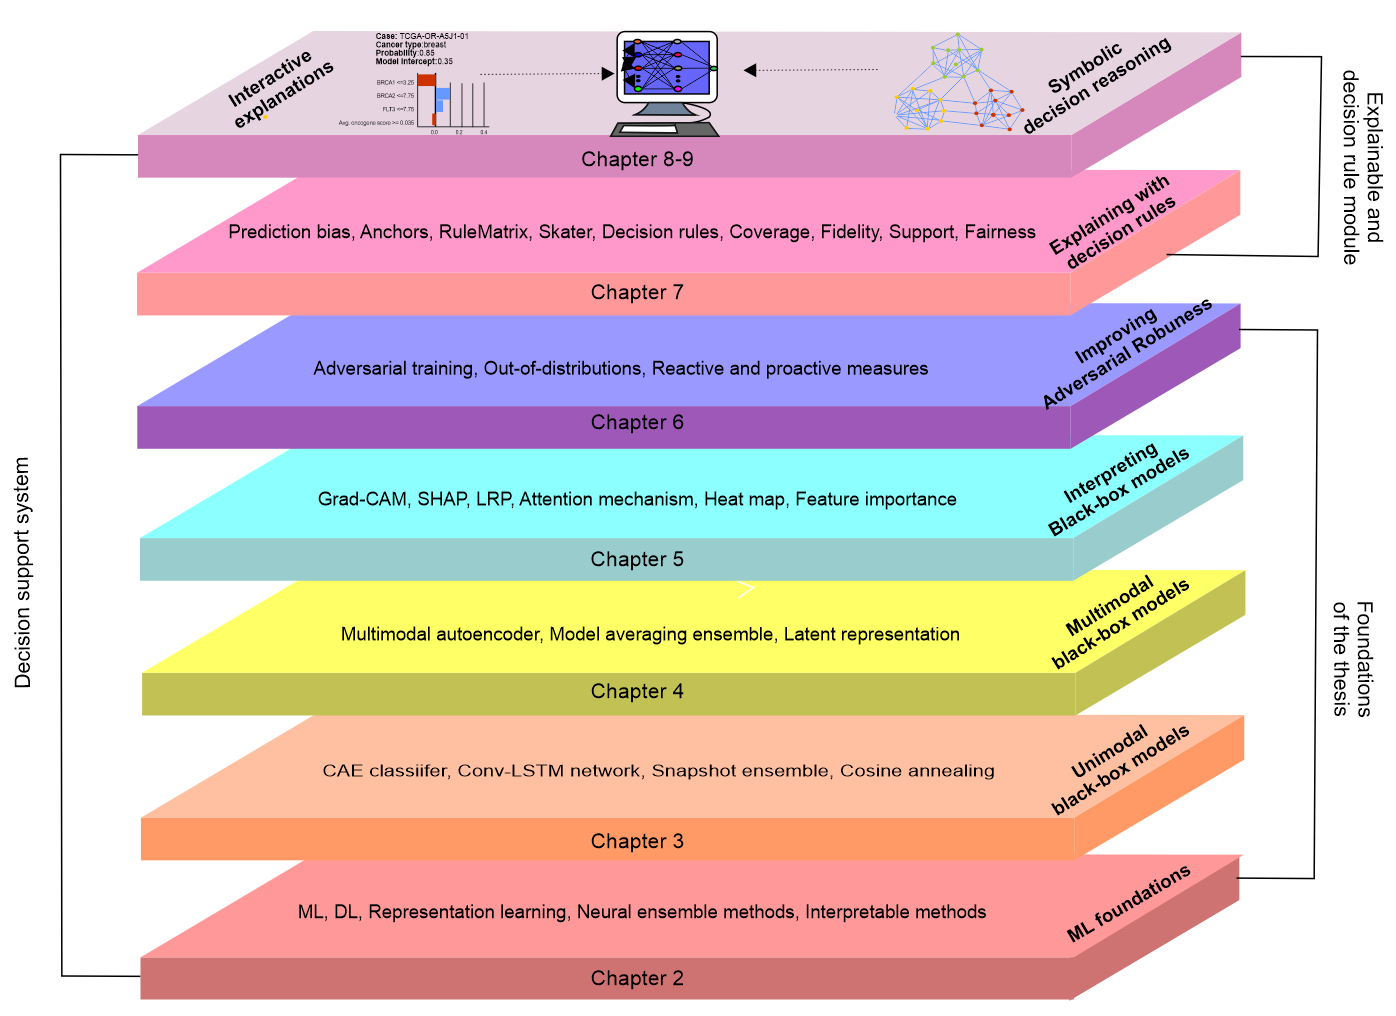
\includegraphics[width=0.8\linewidth,height=105mm]{images/chapter_outline.png}
		\caption{A bottom-up layout of the thesis, outlining the chapters}
        \label{fig:chapter_organization}
\end{figure*}

\section{Thesis Outline} \label{structure}
The rest of the thesis is structured into ten chapters. 
%The brief overview of each chapter is as followed: 
\Cref{chapter:preli} covers the foundations and concepts that will be used in the subsequent chapters. In \cref{chapter:uni_modality}, we develop predictive model based on single modality towards finding the association between CNV data and cancer, followed by the cancer type prediction task. In \cref{chapter:multiodality}, we extend the single modality based predictive model to multimodality-based cancer typing method by employing a multimodal neural network, but with a focus on breast cancer. In \cref{chapter:xai}, we employ two different approaches to open the `black box' uni/multimodal models towards making explainable predictions of cancer types based on different genomics data. Besides, we identify significant biomarkers and computed feature importance in terms of mean absolute impact to rank top genes across all the cancer types. In \cref{chapter:robustness}, we apply different types of adversarial attacks on our models, including image content moderation, numeric data moderation, and out-of-distribution, followed by assessing the robustness against these scenarios. 

\hspace*{3.5mm} In \cref{chapter:xai_rules}, we generate decision rules by combining model predictions and interpretations. Additionally, we identify  misclassified instances~(i.e., initial prediction by the model). In \cref{chapter:nsr}, we apply symbolic reasoning to provide diagnosis reasoning based on a domain-specific ontology; where, a reasoner decides whether a biological entity~(based on biomarkers and their attributes) is of correct types based on the ontological reasoning. The reasoner also help validate the findings and decision rules in order to deduce human-understandable decision rules. In \cref{chapter:fairness}, we improve the trustworthy of the diagnosis by combining model interpretations, decision rules, and decision reasoning. In \cref{chapter:end}, we provide explanations and points out the relevance of the study, highlights its limitations, and discusses future works before concluding the dissertation. 


\chapter{Foundations}
\label{chapter:preli}
\textit{``The beginning of knowledge is the discovery of something we do not understand''}- Frank Herbert 

\section{Chapter Overview}
In this chapter, we cover the foundations and concepts that will be found in all the subsequent chapters. We start with a basic of decision support systems~(DSS) and move towards an intelligent DSS. Subsequently, we cover the necessary foundations for building an explainable DSS for to provide accurate diagnoses decisions about different cancer types. In particular, we cover in detail the concepts of machine learning~(ML) and deep learning~(DL), artificial intelligence~(AI), decision rules, neuro-symbolic reasoning, and representation learning~(RL), with a focus on explainability and algorithmic transparency. Later in the chapter, we discuss different types and subtypes of cancer, growth and metastasis of cancer, in order to know the biological interpretations of genomics data. 

\section{Decision Support Systems}\label{sec:DSS}
Decision support systems~(DSS) are information system that support business or organizational decision-making activities~\cite{hackathorn1981organizational}. A typical DSS takes a set of input and analyzes them to generate actionable insights and recommendation based on which `decisions' are generated. 
In other words, DSSs are often computerized program that analyse massive amounts of data to assists in decision-making. 
However, a real-world DSS may require additional consideration and analysis of multiple criteria features which, in turn, affect the final decisions.  Criteria are often conflicting in nature. For example, in the case of investing in share market, factors such as companies profile and current trend, price, market volatility, and socio-economic or political situation all come into consideration. 

\hspace*{3.5mm} Therefore, to improve the quality and accuracy of the intended decisions, scientific approaches often necessary to perform complex evaluation and validation in the critical decision-making process. Nevertheless, a decision may need be decision can be further validated with user knowledge and expertise. Knowledge base~(KB), predictive models~(decision context and user criteria), and the user interface are three fundamental components of a DSS architecture~\cite{hackathorn1981organizational}. Besides, users themselves play important role in the overall decision-making process, particularly by providing input and out specification and domain-knowledge in the validation stage. DSS components can be broadly classified as follows~\cite{hackathorn1981organizational}: 

\iffalse 
\vspace{-2mm}
\begin{enumerate}[noitemsep]
    \item  \textbf{Inputs}: Factors, numbers, and characteristics to analyze.
    \item \textbf{Knowledge base}: Inputs requiring manual analysis by the user.
    \item \textbf{Outputs}: Transformed data from which DSS "decisions" are generated.
    \item \textbf{Decisions}: Results generated by the DSS based on user criteria.
\end{enumerate}
\vspace{-2mm}
\fi 

Haettenschwiler et al.~\cite{haettenschwiler1999neues} differentiates three types of DSS called passive, active, and cooperative DSS:  

\vspace{-2mm}
\begin{itemize}[noitemsep]
    \item \textbf{Passive DSS} - help in the decision-making process, but cannot provide explicit decision suggestions.
    \item \textbf{Active DSS} - provides decision suggestions or solutions. 
    \item \textbf{Cooperative DSS} - allows iterative process between human and the DSS system itself towards achieving a consolidated solution.
\end{itemize}
\vspace{-2mm}

\hspace*{3.5mm} A cooperative system, thus, has several advantages over active and passive DSS. For example, using a cooperative DSS, decision makers can modify or refine the decision suggestions provided by the system, before sending them back to the system for validation~\cite{hackathorn1981organizational}. Subsequently, the system again improves, completes, and refines the suggestions of the decision maker and sends them back to them for validation. Secondly, the presence of human-in-the-loop, help improve human-AI interaction towards achiving an intelligent DSS. In terms of mode of assistance, communication-driven, data-driven, document-driven, knowledge-driven, and model-driven DSSs can be developed~\cite{power2002decision}:

\vspace{-2mm}
\begin{itemize}[noitemsep]
    \item \textbf{Communication-driven DSS} - used to leverage supports for multiple users working on a shared task collaboratively, particularly targeting at internal teams and their partners. Web or client server via chats and instant messaging software are most common technology used to deploy to leverage online collaboration and net-meeting systems like Google Docs. 
    \item \textbf{Data-driven DSS} - used to provide access to and manipulation of internal or external company data, such that organizational staff can query a database or data warehouse to seek specific answers to specific questions. This types of DSSS were conventionally deployed via a mainframe computer, client-server system, or on the web. 
    \item \textbf{Document-driven DSS} - used to search, manage, retrieve, and manipulate unstructured information via web pages~(i.e., often client-server architecture) that are stored in a variety of formats. 
    \item \textbf{Knowledge-driven DSS} - used to provide specialized problem-solving expertise based on domain-knowledge. In knowledge-driven DSSS, facts, rules, procedures or in similar structures like interactive decision trees and flowcharts, often form the foundation of the KB. 
    \item \textbf{Model-driven DSS} - used to leverage access to and manipulation of a statistical, financial, or simulation model. Model-driven DSS use data and parameters provided by users to assist decision makers in analyzing a situation. However, they are not necessarily data-intensive. 
\end{itemize}
\vspace{-2mm}
%However, DNN models are perceived mostly as `black box' methods because of their not well-understood internal functioning. Besides, they cannot reason their underlying decisions, leaving them incapable of aiding transparent and trustworthy decisions. Consequently, we call such DSS a `black box' model. 

%This chapter provides a general introduction to this dissertation, provides the motivation for this research, list down the hypotheses and research questions, and outlines the structure of this thesis. 

\hspace*{3.5mm} The expert systems based on collections of `if-then' rules were the dominant technology for AI in the 1980s~\cite{davenport2019potential}. They were widely employed for `clinical decision support system~(CDSS) purposes over the last couple of decades. Such a DSS require human experts and domain knowledge to generate a set of rules used to provide decision in numerous tasks~\cite{davenport2019potential}. 
As long as there are a few rules in the rule set, they work well and easy to understand. However, when the number of rules is large, including conflicting rules, they tend to break down. Moreover, if the underlying domain knowledge changes, updating the rules can be difficult and time consuming~\cite{davenport2019potential}. Moreover, rule-based clinical DSS are difficult to maintain as medical knowledge changes and are often not able to handle the explosion of data and knowledge based on genomic, proteomic, metabolic and other ‘omic-based’ approaches to care~\cite{das2020opportunities}.
Subsequently, they gradually being replaced with ML-based systems with AI capabilities. 

\hspace*{3.5mm} DSSs that can perform selected cognitive decision-making functions based on artificial intelligence~(AI) or intelligent agents technologies called intelligent DSS. Due to recent advancement and performance across domains like computer vision, natural language processing, multimedia analytics, and business analytics, an AI-guided DSS could eventually be applied to various automated decision-making processes~\cite{davenport2019potential}.  In an AI-guided or intelligent DSS, a set of learning algorithms are embedded to perform cognitive decision-making in which ML often act as one of the most common forms of AI~\cite{das2020opportunities}. An intelligent DSS is often ML or DL-based DSS, where a ML or DL algorithm is employed to improve the learning outcome so that the decision-making process becomes automatic by reducing the level of human interaction as much as possible~\cite{davenport2019potential}. 
In this thesis, we aim at developing an intelligent DSS by leveraging both data-, knowledge-, and model-driven characteristic; such that an ML model trained on the data forms the foundations of the DSS's decision making process and the domain-knowledge will be used to aid the users to validate the outcome. Nevertheless, since the `black-box' nature and opaqueness in predictive model raises numerous legal, ethical, and practical concerns, we aim to improve the transparency and explainability of the DSS. In the subsequent sections, we discuss some fundamental components required to develop the DSS such as ML, DL, RL, multimodal learning, interpretability, and different types of data required. 

\section{Machine Learning}
ML is about using a set of statistical and mathematical algorithms to perform tasks such as concept learning, predictive modeling, clustering, and mining useful patterns can be performed, where a learner or ML algorithm is the program used to learn a ML model from data. Subsequently, a ML model is the learned program that maps inputs to predictions. Tom M. Mitchell~\cite{mitchell1997machine} explained what learning really means from a computer science perspective: \textit{``a computer program is said to learn from experience $E$ with respect to some class of tasks $T$ and performance measure $P$, if its performance at tasks in $T$, as measured by $P$, improves with experience $E$"}. We can interpret the above definition in another way: based on a set of observation or data~(i.e., experience $E$), a learning algorithm can be used to solve a problem~(i.e., task $T$) iteratively, i.e., as long as the performance~(i.e., $P$) is not satisfactory. 

\hspace*{3.5mm}Based on this interpretation, a machine can learn from data/observations and can be improved with experience to predict an outcome more accurately. When it comes to data, what we mean is a set of features/inputs and targets from which the machine learns. Subsequently, a learned program called a ML model can map inputs to predictions. The resultant is weights for a linear model or for a neural network~(we'll shortly discuss about). Training a ML model is an optimization problem, where the objective is finding a minimizer of a convex function $f$ and a weight vector $w$ on $d$ data points. Subsequently, we can formulate the learning task as $\min _{w \in \mathbb{R}^{d}} f(w)$, where the objective function is as follows~\cite{karim2018scala}:

\vspace{-4mm}
\begin{align}
    f(w):=\lambda R(w)+\frac{1}{n} \sum_{i=1}^{n} L\left(w ; x_{i}, y_{i}\right)
\end{align}

\hspace*{3.5mm} We call the method linear if $L(w;x,y)$ can be expressed as a function of $w^Tx$ and $y$. The objective function $f$ has two components, i) a regularizer that controls the complexity of the model, ii) the loss that measures the error of the model on the training data. The loss function $L(w;)$ is typically a convex function in $w$. The fixed regularization parameter $\lambda \geq 0$ defines the trade-off between minimizing the loss on the training error and minimizing model complexity to avoid overfitting~\cite{karim2018scala}. If both of components are convex, their sum is also convex, else non-convex~\cite{zaccone2018deep}. Therefore, using a convex optimization technique, we can minimize the function until it converges towards the minimum error.  %This can be a set of weights for a linear model or for a neural network. Other names for the rather unspecific word "model" are "predictor" or - depending on the task - "classifier" or "regression model". he trained ML model is called $\hat{f}$ or $\hat{f}(x)$

\begin{figure}[h]
	\centering
	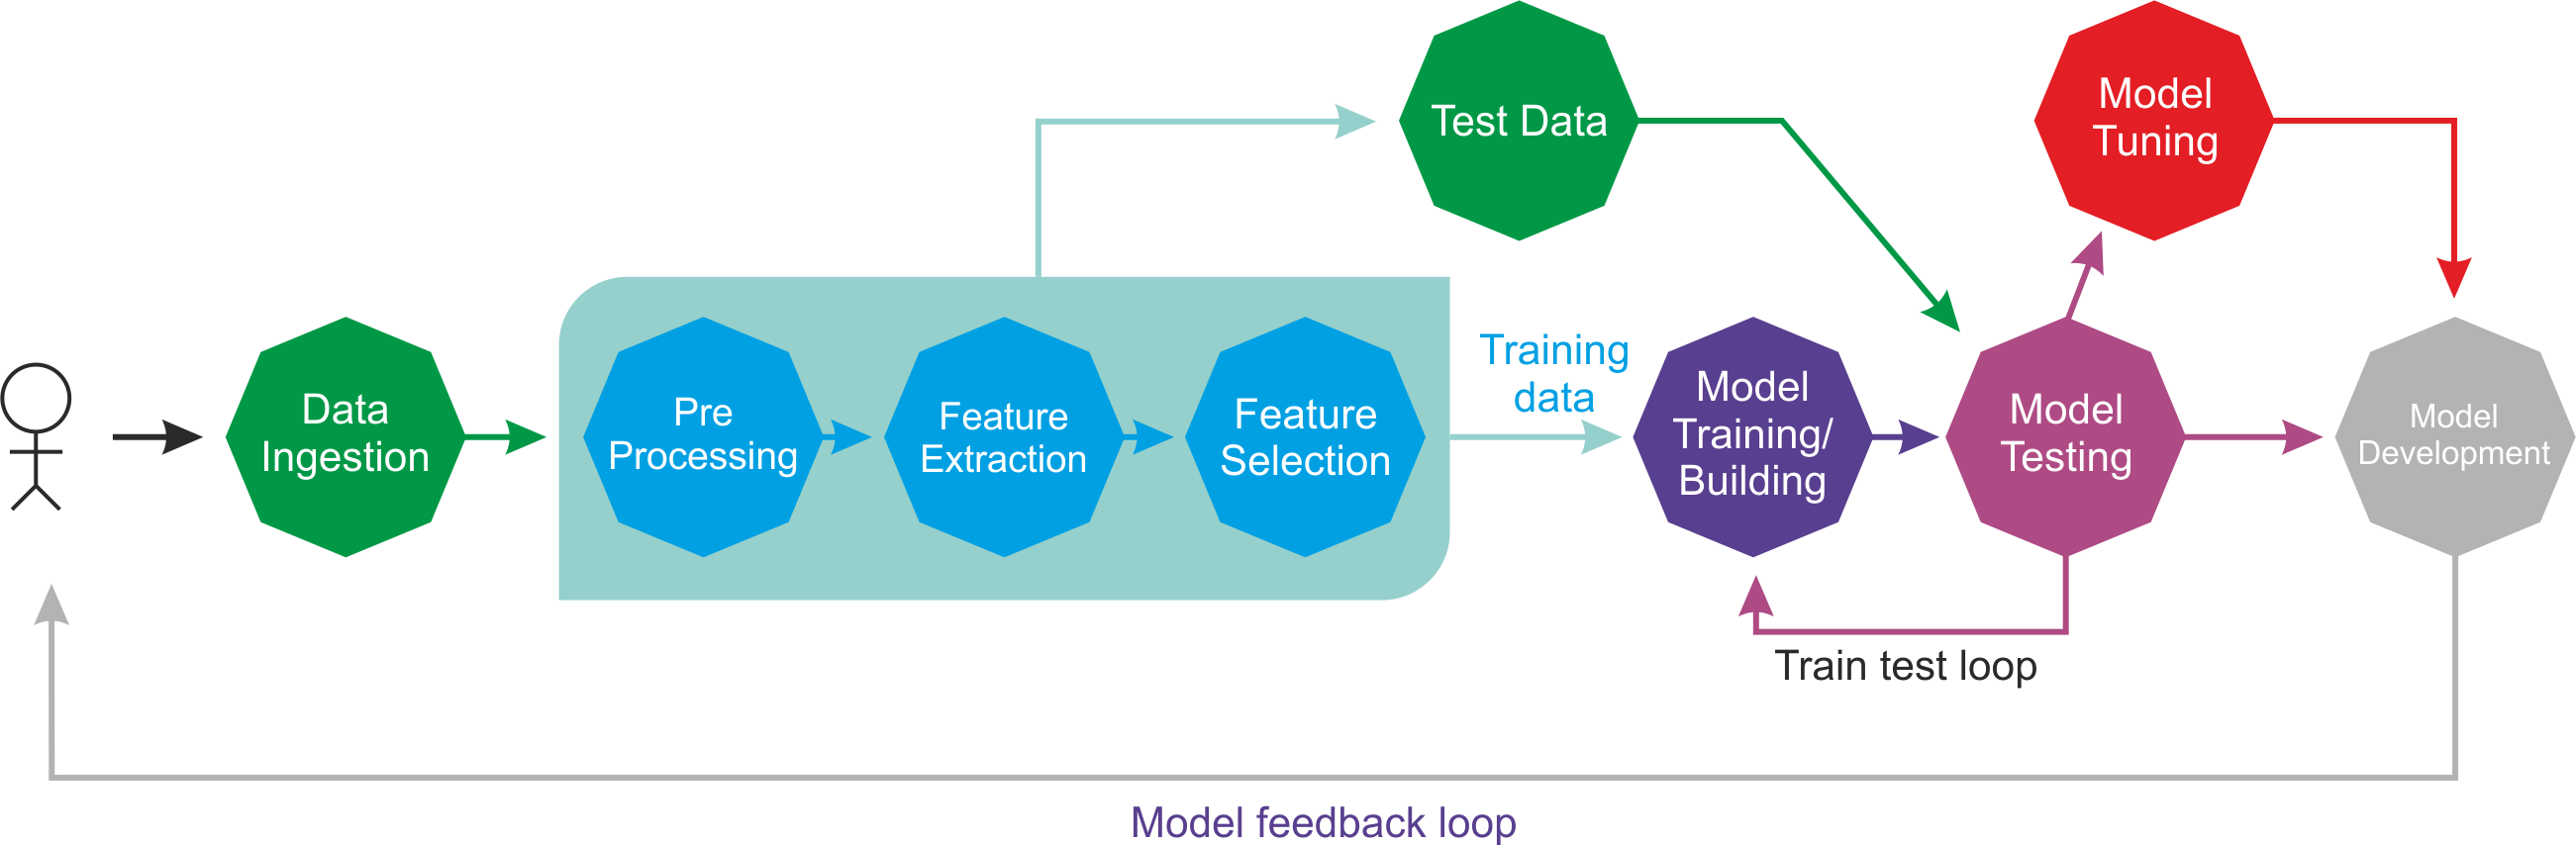
\includegraphics[width=0.9\linewidth,height=60mm]{images/B08452_01_02.png}
	\caption{Lifecycle of a typical ML pipeline~\cite{karimScalaML2019}} 
	\label{fig:ml_pipeline}
\end{figure}

\hspace*{3.5mm} The regularization parameter defines the trade-off between minimizing the training error and the model's complexity in an effort to avoid overfitting problems. More elaborately, when using an ML algorithm, the goal is to obtain the best hyperparameters of a function that return the minimum error when making predictions. 
%Given that a problem is convex, it is usually easier to analyze the asymptotic behavior of the algorithm, which shows how fast it converges as the model observes more and more training data. 
The challenge of ML is to allow training a model so that it can recognize complex patterns and make decisions not only in an automated way but also as intelligently as possible. 
However, if the performance is not satisfactory, additional tuning or retraining would be necessary to get the best model, before % based on hyperparameter optimization.
deploying the best model in a production-ready environment. 
\Cref{fig:ml_pipeline} summarizes these steps in a nutshell. Following are a few commonly used terminologies in ML: 

\begin{itemize}[noitemsep]
    \item \textbf{An instance} is a row in the dataset~(also called data point, example, or observation). An instance consists of the features $x^{(i)}$ and~(if known) the target outcome ${y}$, where target is the information that the model learned to predict.

    \item \textbf{Prediction} is what a ML model ``guesses" what the target value should be based on the given feature, i.e., $\hat{y}$ = $\hat{f}\left(x^{(i)}\right)$. If $\hat{y}$ is equal to~(or close) ${y}$, we say it's an accurate prediction.   
\end{itemize}

\subsection{Machine learning tasks}
Although every ML problem is more or less an optimization problem, the way they are solved can vary. Depending on the data type~(often combination of features and targets), learning tasks could be of different three types such as supervised, unsupervised, and reinforcement learning. Supervised learning is the simplest and most well-known automatic learning task. It is based on a number of predefined examples, in which the category to which each of the inputs should belong is already known, as shown in \cref{fig:ml_pipeline_sup}:

\begin{figure}[h]
	\centering
	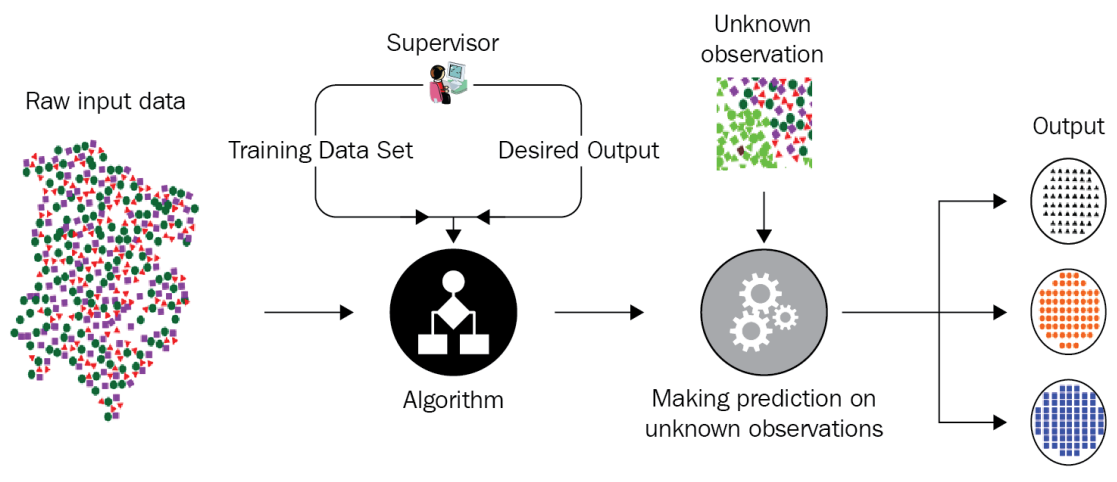
\includegraphics[width=0.9\linewidth,height=50mm]{images/sup.png}
	\caption{Workflow of supervised learning technique~\cite{karimScalaML2019}} 
	\label{fig:ml_pipeline_sup}
\end{figure}

\hspace*{3.5mm} In the preceding diagram, an actor~(e.g., data scientist) performs extraction, transformation, and load~(ETL) and necessary feature engineering~(such as feature extraction, selection, etc.) to get the appropriate data consisting of features and labels, to fed into the model. The training set is used to train a ML model and the validation set is used to validate the training against the overfitting problem and regularization. Then the actor can evaluate model's performance on the test set~(i.e., unseen data). The supervised learning context includes classification and regression. While classification is used to predict which class a data point is a part of discrete value or the label of the class attribute, whereas regression is used for predicting continuous values and making a numeric prediction of the class attribute.

\hspace*{3.5mm} How would you summarize and group a dataset if the labels were not given? Probably, you'll try to answer this question by finding the underlying structure of a dataset and measuring the statistical properties such as frequency distribution, mean, standard deviation, and so on. If the question is how would you effectively represent data in a compressed format? You'll probably reply saying that you'll use some software for doing the compression, although you might have no idea how that software would do it. \Cref{fig:ml_pipeline_unsup} shows the typical workflow of an unsupervised learning task. 

\begin{figure}[h]
	\centering
	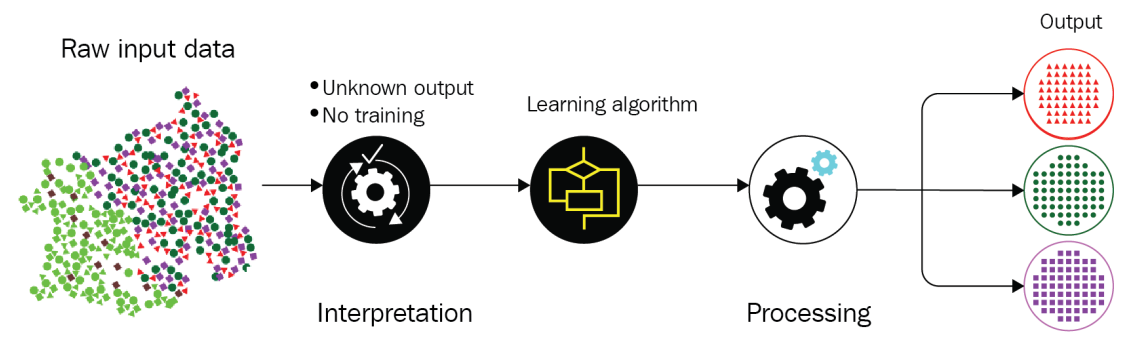
\includegraphics[width=0.9\linewidth,height=50mm]{images/unsup.png}
	\caption{Workflow of unsupervised learning technique~\cite{karimScalaML2019}} 
	\label{fig:ml_pipeline_unsup}
\end{figure}

\hspace*{3.5mm} On the other hand, reinforcement learning focuses on the learning of the system through its interactions with the environment, where system's parameters are adapted based on the feedback obtained from the environment, which in turn provides feedback on the decisions made by the system. On the other hand, another most complex forms of ML involve deep learning~(DL), or deep neural network~(DNN) models with many levels of features or variables that predict outcomes that help take meaningful decision. We will discuss about DL and DNN in subsequent sections. 

%The following diagram shows a person making decisions in order to arrive at their destination. 

%After necessary preprocessing and feature engineering, a common practice is splitting the input data into 60\% for the training, 10\% for the validation, and 20\% for testing, but it depends on use cases. \hspace*{3.5mm} Besides, up-sampling or down-sampling may require in case of class imbalanced scenario. In practice and from the application point of view, a typical ML application involves several processing steps, from the input to the output, forming a scientific workflow as shown \cref{fig:ml_pipeline}. 

\iffalse
\subsection{Role of data in machine learning}
Data in any ML pipeline is a first-class citizen and play key role. The performance of any learning depends on quality features. Depending upon the learning tasks, often we may have to split the data, e.g., in supervised learning tasks, the entire learning process requires input datasets to split into different sets~\cite{karim2018java}:

\vspace{-1mm}
\begin{itemize}[noitemsep]
    \item \textbf{Training set:} is the knowledge base coming from historical or live data used to fit the parameters of the ML algorithm. During the training, the model utilizes the training set to find optimal weights of the network and reach the objective function by minimizing the training error~\cite{karim2018java}. 
    \item \textbf{Validation set:} is a set of examples used to tune the parameters of an ML model to ensure that the model generalizes towards avoiding overfitting~\cite{karim2018java}. 
    \item \textbf{Test set:} is used for evaluating the performance of the trained model on unseen data. This step is also referred to as model inferencing. After assessing the final model on the test set, no need to tune the model before deploying in a production-ready environment~\cite{karim2018java}.
\end{itemize}
\vspace{-1mm}

\hspace*{3.5mm} In the context of supervised learning, the learning process required for the input dataset is split randomly into three sets, for example, $60\%$ for the training set, $10\%$ for the validation set, and the remaining $30\%$ for the testing set.
\fi 

\section{Deep Learning and Neural Networks}
Deep neural networks~(DNNs) form the core of deep learning~(DL) by providing a set of algorithms to model complex and high-level abstractions in data and can better exploit large-scale datasets to build complex models, and have been widely used in computer vision, speech recognition, NLP, social network, machine translation, bioinformatics, etc. Layers in a neural network is composed of a set of artificial neurons called perceptron~\cite{yuan2019adversarial}. A perceptron maps a set of inputs to outputs with a special function called activation functions. Multiple such layers are stacked to create such a neural network. 

\hspace*{3.5mm} Till date, numerous neural network architectures have been proposed and are in use. We can categorize DL architectures into four groups: i) feed-forward neural networks~(FFNNs), ii) Convolutional neural networks~(CNNs), iii) Recurrent neural networks~(RNNs), iv) Autoencoders~(AEs), and v) Emergent architectures. However, FFNNs, CNNs, AEs, and RNNs have many improved variants. Although most of the variants are proposed or developed for solving domain-specific research problems, the basic working principles still follow the original  architectures. In this section, we provide preliminaries and theoretical foundations of these architectures that are used throughout in the subsequent chapters.  

\subsection{Feed-forward neural networks}
Feed-forward neural networks~(FFNNs) are neural networks that have a complex and deeper architecture with a large number of neurons in each layer, and many connections between them. Although DNN refers to a very deep network, for simplicity, we consider MLP, stacked autoencoder~(SAE), and deep belief networks~(DBNs)~\cite{Hinton:2009} as DNN architectures. These architectures mostly work as an FFNN, meaning information propagates from input to output layers. Multiple perceptrons are stacked together as MLPs, where layers are connected as a directed graph. Fundamentally, an MLP is one of the most simple FFNNs since it has three layers as shown in \cref{fig:mlp_1}: an input layer, a hidden layer, and an output layer, where the signal propagates one way, from the input layer to the output layer as shown in \cref{fig:mlp_1}.

\hspace*{3.5mm} However, it is not possible to determine a priori, with adequate precision, the required number of hidden layers, or even the number of neurons that must be contained inside each hidden layer to compute a non-linear function. There is no straightforward answer to this, but we can try increasing the number of neurons in a hidden layer until the FFNN starts overfitting. We will discuss this later on. Despite some rules of thumb, setting the number of hidden layers relies on experience and on some heuristics to determine the structure of the network. If a low number of hidden layers, or neurons, constitute the neural network architecture, then the network is not able to approximate with adequate precision the unknown function, for example. This could be because it is too complex, or because the backpropagation algorithm falls within a local minimum. If the network is composed of a high number of hidden layers, then we have an overfitting problem. One solution to this problem is regularization through dropout. Therefore, a complex network can consist of many neurons, hidden layers, and connections, but in general, an ANN with two or more hidden layers is called a DNN. From the implementation perspective, a DNN can be constructed by stacking multiple ANNs together~\cite{karimDLTF2018}.

\begin{figure}[h]
    \centering
    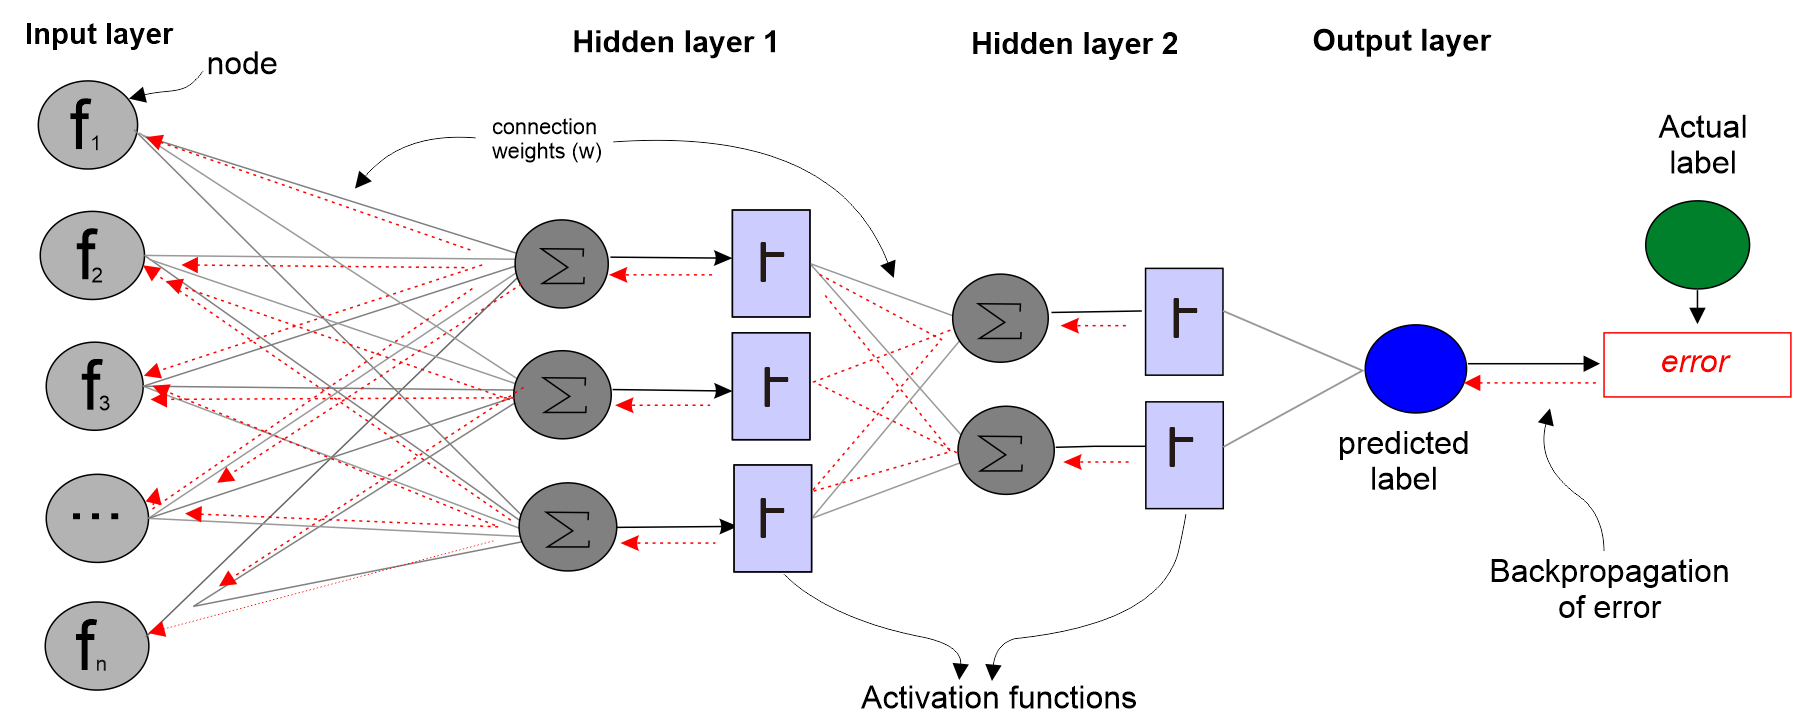
\includegraphics[width=0.9\textwidth,height=65mm]{images/ffnn_1.png}
    \caption{The architecture of a MLP with an input layer, 2 hidden layers, and an output layer}
    \label{fig:mlp_1}
\end{figure}

\hspace*{3.5mm} RBMs are the basic building blocks for DBNs. Unlike MLP, which is an FFNN that's trained in a supervised way, DBNs are trained in two phases: unsupervised pretraining and supervised fine-tuning. In unsupervised pretraining, layers are stacked in order and trained in a layer-wise manner with used unlabeled data. In supervised fine-tuning, an output classifier layer is stacked and the complete neural network is optimized by retraining with labeled data. One problem with MLP is that it often overfits the data, so it doesn't generalize well. To overcome this issue, DBN was proposed , which uses a greedy, layer-by-layer, pretraining algorithm and composed of a visible layer and multiple hidden unit layers. However, despite numerous successes, DBNs have been replaced with AEs. 

\subsection{Autoencoders}
\label{preli:AEs}
A regular AE consists of multi-layer dense networks called encoder and decoder, which is architecturally an MLP~\cite{karimDLTF2018}. AE also acts data compression technique where the compression and decompression functions are data-specific, lossy, and learned automatically from samples rather than human-crafted manual features~\cite{karimDLTF2018}. The encoder learns the representation of input $X$ in a compressed format in which the data is mapped and transformed into an embedding $Z$.  

\begin{figure}[h]
    \centering
    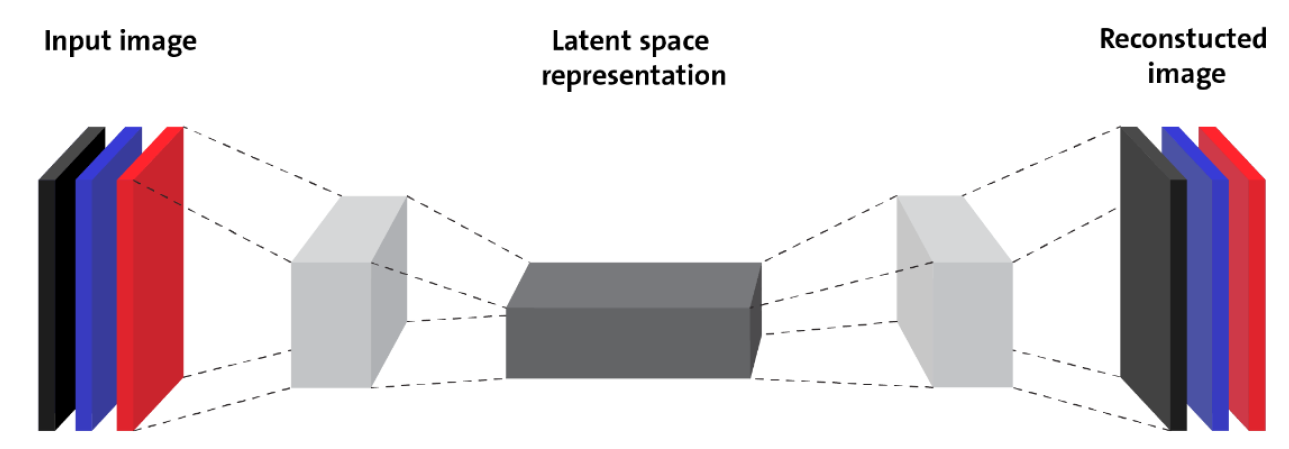
\includegraphics[width=0.55\textwidth,height=65mm]{images/ae.png}
    \caption{An unsupervised autoencoder as a network for latent feature learning~\cite{karimDLTF2018}}
    \label{fig:ae_theory1}
    \vspace{-2mm}
\end{figure}

%The decoder module of the AE network maps $Z$ to the reconstruction $X^{\prime}$~\cite{karimACCESS2019}, i.e., by approximating a function, $h_{W, b}(x) \approx x$, the decoder module to the identity function in order to output $\chi^{\wedge}$, which is similar original input x. 
\hspace*{3.5mm} Then the decoder tries to reconstruct $X$ from $Z$ by reducing the reconstruction loss between $X$ and its corresponding reconstruction $X^{\prime} \in \mathbb{R}^{D}$ such that useful information is not lost in the encoding phase~\cite{KarimIEEEAccess2019}.

\vspace{-2mm}
\begin{itemize}[noitemsep]
    \item \textbf{Encoder}: encodes the input into a latent-space representation using function $h = f(X)$.
    \item \textbf{Decoder}: reconstructs the input from the latent space representation using function $\tilde{x} = g(h)$. 
\end{itemize}
\vspace{-2mm}

Usually, reconstruction loss is the distance measure~($d_{AE}$) between input $x_i$ and network's output $f(x_i)$: 

\vspace{-2mm}
\begin{equation}
    L_{AE}=\text{$d_{AE}$}(x_i, f(x_i) = \sum_{i} ||x_{i}-f(x_i)||^{2}.
    \label{eq:Loss1}
\end{equation}

\hspace*{3.5mm} The identity function seems a particularly trivial function to be trying to learn, but by placing constraints on the network, such as by limiting the number of hidden units, we can discover interesting features of the data~\cite{karimDLTF2018}. Although used for learning representations from numeric data and LQ images, AE is mostly not suitable for 2D/3D finite and discrete signals or digital images~\cite{min2018survey}, primarily because of their weak RL capability. In \cref{sec:rep_learn}, we discuss different variants of autoencoders for the RL. %, which we will use in subsequent chapters. 

\subsection{Convolutional neural networks}
DNNs have no prior knowledge of how the pixels are organized because they do not know that nearby pixels are close. CNNs embed this prior knowledge using lower layers by using feature maps in small areas of the image, while the higher layers combine lower-level features into larger features. This setting works well with most of the natural images, giving CNN a decisive head start over DNNs~\cite{karimIoT2019}. CNNs have achieved much and have been widely adopted in computer vision, e.g., image recognition. The connection schemes in a CNN are significantly different compared to an MLP or DBN. A few of the convolutional~(conv) layers are connected in a cascade style. 

\begin{figure}[h]
    \centering
    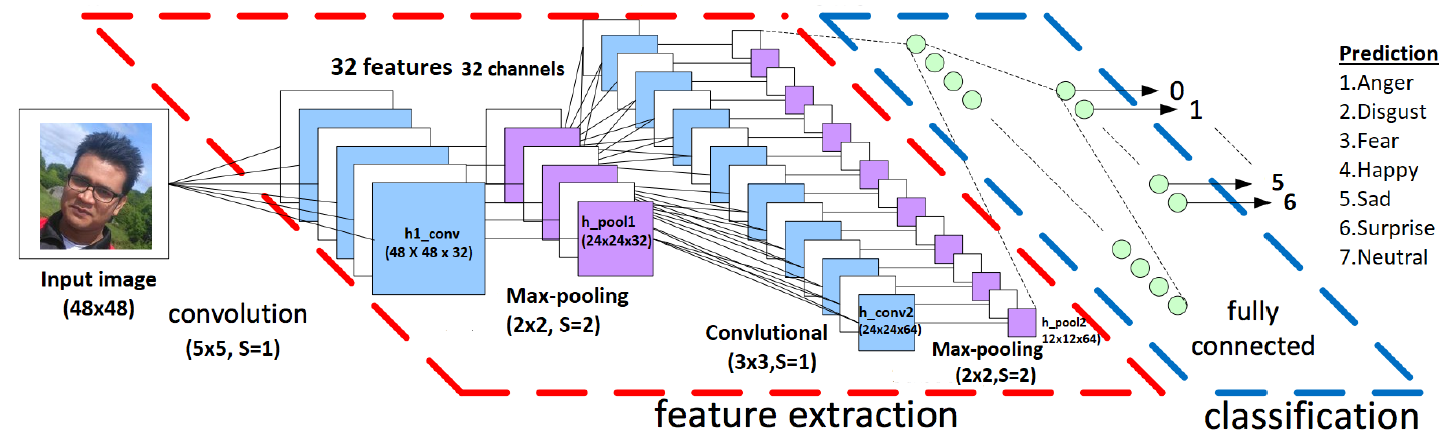
\includegraphics[width=0.9\textwidth,height=50mm]{images/cnn.png}
    \caption{A schematic architecture of a CNN used for facial recognition~\cite{karim2017predictive,zaccone2018deep}}
    \label{fig:cnn_theory1}
\end{figure}

\hspace*{3.5mm} The output from each conv layer is a set of objects, called feature maps generated by a single kernel filter. Then, the feature maps can be used to define a new input to the next layer. Each neuron in a CNN network produces an output followed by an activation threshold, which is proportional to the input and not bound. Each layer is backed up by an ReLU layer, a pooling layer, additional conv layers (+ReLU), and another pooling layer, which is followed by a fully connected layer~(FCL) and a softmax layer. The preceding diagram~(\cref{fig:cnn_theory1}) is a schematic architecture of a CNN used for facial recognition, which takes facial images as input and predicts emotions such as anger, disgust, fear, happy, and sad~\cite{karimDLTF2018}.  
%A neuron can be active (or firing) if its output value is close to 1, or inactive if its output value is close to 0. However, for simplicity, we assume that the neurons are inactive most of the time. This argument is true as long as we are talking about the sigmoid activation function. However, if you are using the tanh function as an activation function, then a neuron is inactive when it outputs values close to -1.

\subsection{Recurrent neural networks}
Traditional neural networks instead ignore past events, as it is not possible for a neural network to use past scenes to classify current ones. In contrast to conventional neural networks, RNNs are networks with a loop that allows the information to be persistent in a neural network. The backpropagation time rolls out the RNN, creating a very deep feed-forward neural network. The impossibility of getting a long-term context from the RNN is due precisely to this phenomenon: if the gradient vanishes or explodes within a few layers, the network will not be able to learn high temporal distance relationships between the data. 

\begin{figure}[h]
    \centering
    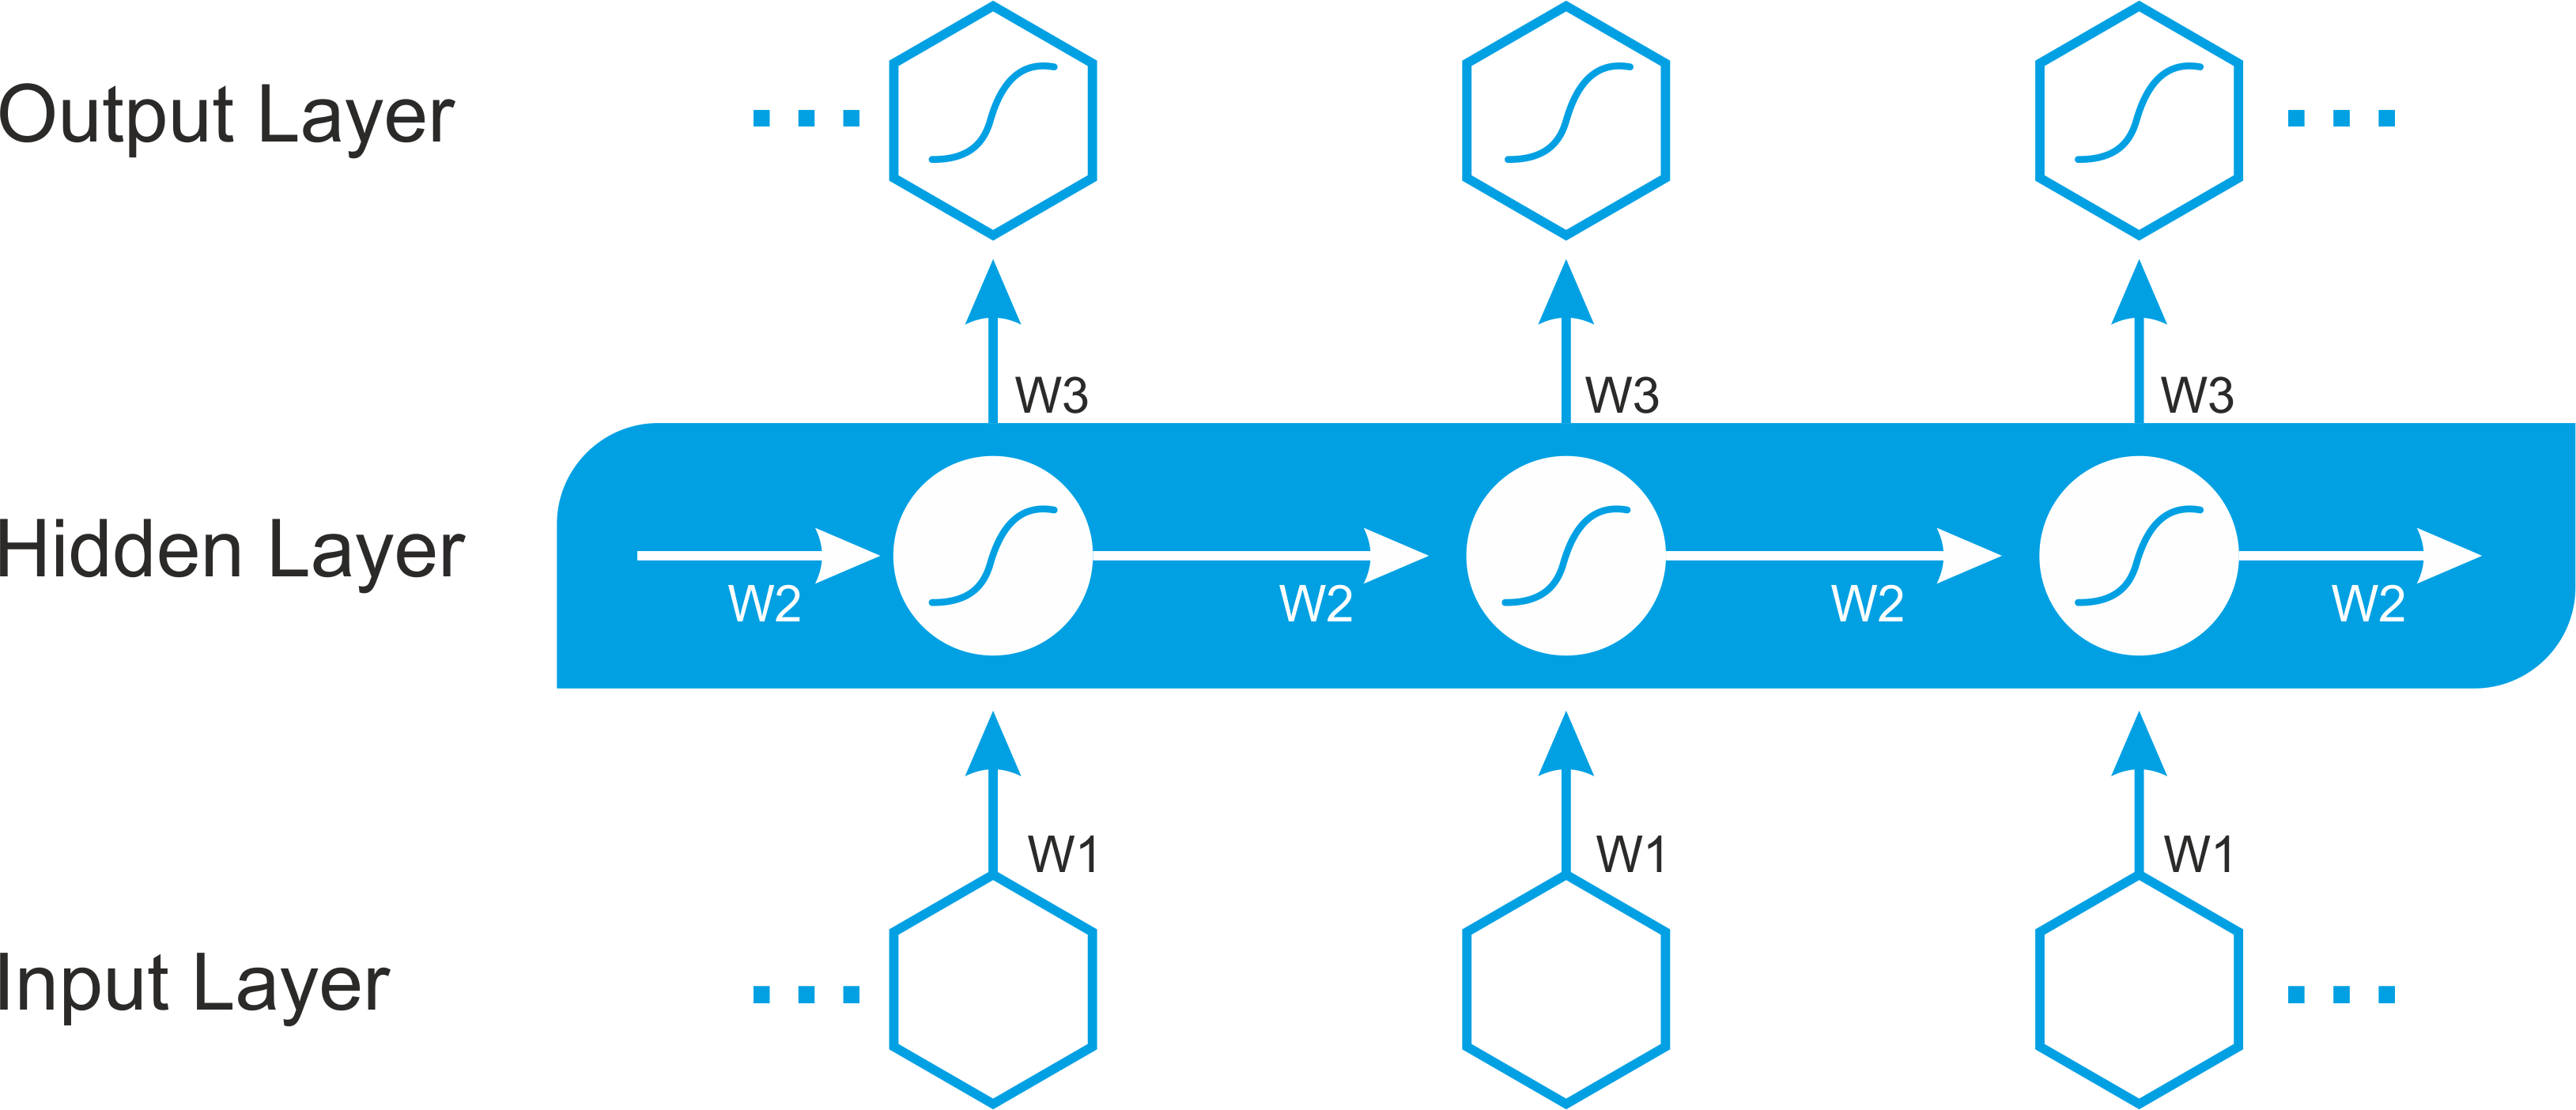
\includegraphics[width=0.7\textwidth,height=45mm]{images/B09698_06_4.png}
    \caption{In RNN all the weights in all the layers have to be learned with time~\cite{karimDLTF2018}}
    \label{fig:rnn_theory1}
    \vspace{-2mm}
\end{figure}

\hspace*{3.5mm} The preceding diagram~(\cref{fig:rnn_theory1}) is a schematic architecture of a RNN, where all the weights in all the layers have to be learned with time~\cite{karimDLTF2018}. However, the computed and back-propagated gradient tends to decrease~(or increase) at each instant of time and then, after a certain number of instants of time, the cost function tends to converge to zero (or explode to infinity). However, improved RNN variants such as LSTM, bi-directional LSTM, and GRU can combat the vanishing gradients and offers excellent results and performance. LSTM-based networks are ideal for the prediction and classification of temporal sequences and are replacing many traditional approaches to DL. As the name signifies, that short-term patterns are not forgotten in the long term. 

\subsection{Emergent architectures}
Many other emergent DL architectures have been suggested, such as Redidual networks~(ResNets), Deep SpatioTemporal Neural Networks~(DST-NNs), Multi-Dimensional Recurrent Neural Networks~(MD-RNNs), and densely-connected neural networks~(DenseNet). Other neural networks such as CapsNets - an improved version of a CNN, RNN for image recognition, and Generative Adversarial Networks~(GANs) for simple image generation. Apart from these, factorization machines for penalization and DL are also used. 

\iffalse
\subsubsection{Residual neural networks}
Since there are sometimes millions and millions of hyperparameters and other practical aspects, it's really difficult to train deeper neural networks. To overcome this limitation, a residual learning framework is proposed~\cite{zagoruyko2016wide} to ease the training of networks that are substantially deeper than those used previously. They also explicitly reformulated the layers as learning residual functions with reference to the layer inputs, instead of learning non-referenced functions. This way, these residual networks are easier to optimize and can gain accuracy from considerably increased depth. The downside is that building a network by simply stacking residual blocks inevitably limits the optimization ability. %To overcome this limitation, Ke Zhang et al. also proposed using a multilevel residual network.

\subsubsection{Generative adversarial networks}
GANs architectures consist of two networks pitted against each other introduced by Ian Goodfellow et al.~\cite{GAN}. In GANs, two main components are the generator and discriminator. In a GAN architecture, a generator and a discriminator are pitted against each other—hence the name - adversarial~\cite{GAN}:

\vspace{-2mm}
\begin{itemize}[noitemsep]
    \item \textbf{Generator}: the generator tries to generate data samples out of a specific probability distribution and is very similar to the actual object.
    \item \textbf{Discriminator}: the discriminator will judge whether its input is coming from the original training set or from the generator part. 
\end{itemize}

\vspace{-2mm}
\begin{figure}[h]
    \centering
    \vspace{-3mm}
    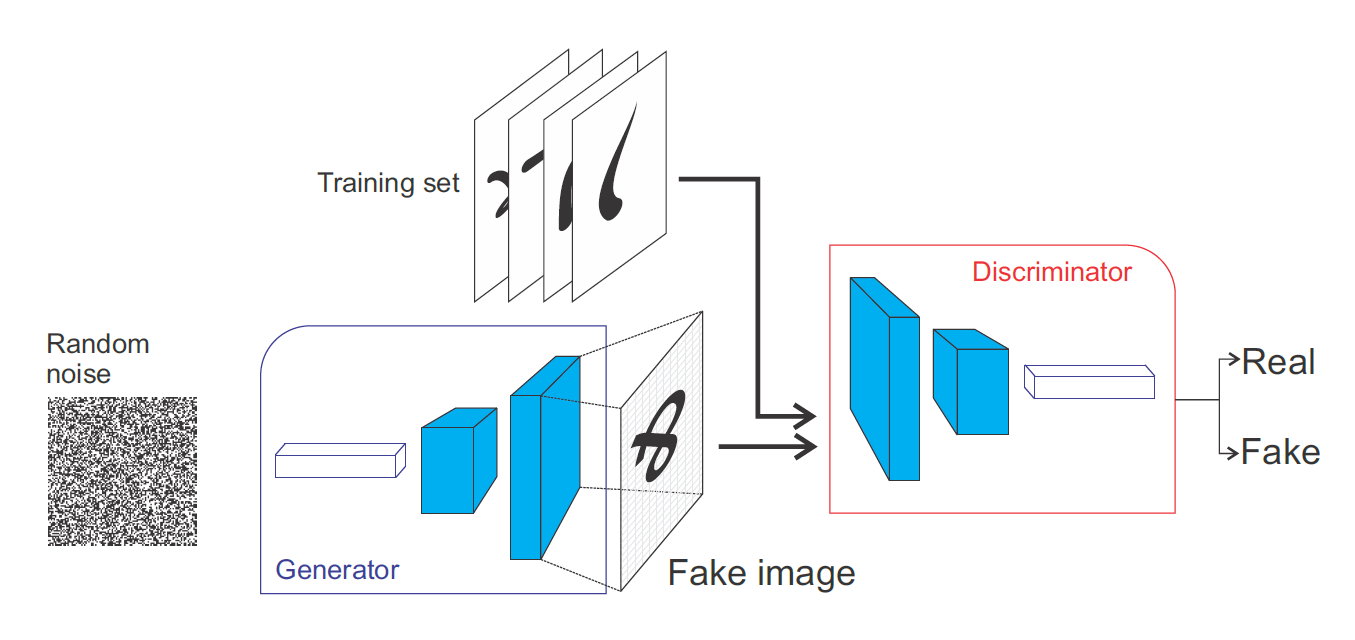
\includegraphics[width=0.75\textwidth,height=50mm]{images/gan.png}
    \caption{Schematic diagram of a simple GAN~\cite{karimDLTF2018}}
    \label{fig:gan}
    \vspace{-2mm}
\end{figure}

\hspace*{3.5mm} \Cref{fig:gan} shows a schematic diagram of a simple GAN. Many DL practitioners think that GANs were one of the most important advancements because GANs can be used to mimic any distribution of data, and, based on the data distribution, they can be taught to create robot artist/super-resolution images, text to image synthesis, speech. Facebook's AI research director, Yann LeCun, thinks GANs are the most interesting idea in the last 10 years of ML\footnote{See: Generative Adversarial Networks: What Are They and Why We Should Be Afraid, by Thomas Klimek, 2018}.

\subsubsection{Capsule networks}
In CNNs, each layer understands an image at a much more granular level through a slow receptive field or max pooling operations. If the images have rotation, tilt, or very different shapes or orientation, CNNs fail to extract such spatial information and show very poor performance at image processing tasks. Even the pooling operations in CNNs cannot be much help against such positional invariance. This issue in CNNs has led CapsNet~\cite{CapsNet}, where a capsule is a group of neurons whose activity vector represents the instantiating parameters of a specific type of entity, such as an object or an object part~\cite{CapsNet}.

\begin{figure}[h]
    \centering
    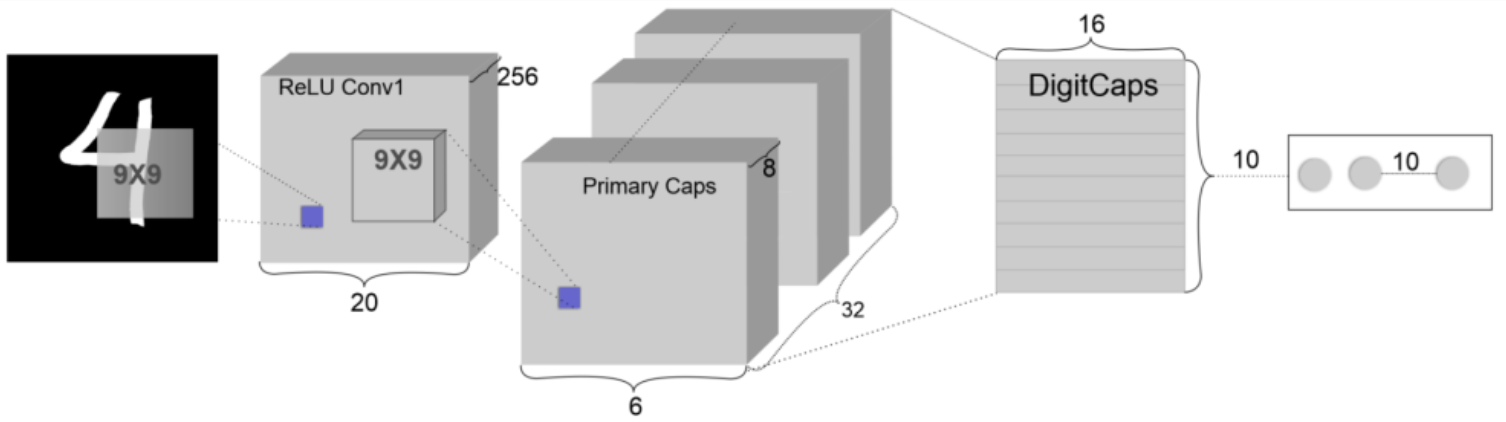
\includegraphics[width=0.9\textwidth,height=40mm]{images/capsnet.png}
    \caption{Schematic diagram of a simple three-layer CapsNet~\cite{karimDLTF2018}}
    \label{fig:capsnet}
\end{figure}

\hspace*{3.5mm} Unlike a regular DNN, where we keep on adding layers, in CapsNet, the idea is to add more layers inside a single layer, making the CapsNet a nested set of neural layers~\cite{CapsNet}. In CapsNet, the vector inputs and outputs of a capsule are computed using the routing algorithm used in physics, which iteratively transfers information and processes the self-consistent field~(SCF) procedure. \Cref{fig:capsnet} shows a schematic diagram of a simple three-layer CapsNet. The length of the activity vector of each capsule in the DigiCaps layer indicates the presence of an instance of each class, which is used to calculate the loss. 
\fi 

\section{Representation Learning}
\label{sec:rep_learn} 
In recent years, DL has been successfully applied to multimodal learning problems, with the aim of learning useful joint representations from different types of data called modality. Modality refers to the way in which we experience a real-life events that includes multiple such modalities~\cite{mmsurvey}. For example, in time series domain available modalities includes video, audio, and sensor signals.
Second example would be visual question answering system or an e-commerce site, where both images and text need to be combined. For the former, it is imperative to consider the temporal structure of individual modalities during the fusion process. For the latter, both images and text descriptions are provided for the customers. 

\hspace*{3.5mm}Representing raw data in a format that a ML model can work with has always been a big challenge in order to develop DSS~\cite{mmsurvey}. Images, audio samples, individual words, or a sentence features are often represented in vector or tensor formats, which is called representation learning~(RL). In many cases, using a single unimodal representation learning is sufficient for each modality in the creation of multimodal space. However, multimodal representations are distributed vectors that map multiple modes of information to a single mathematical space, where distances between instances delineate their similarity~\cite{ito2018effects}. 
In this section, we discuss different RL techniques for both unimodal and multimodal datasets. 

\subsection{Learning representation from unimodal data}
Although the development of unimodal representations has been extensively studied, there has been a shift from hand-designed for specific applications to data-driven~\cite{mmsurvey}. Different neural network architectures have been proposed to improve the quality of the RL~\cite{min2018survey} from multimodal datasets. For example, visual representations based on CNNs and acoustic representations using epectrograms or with autoencoders, are among a few examples where the network learn unimodal features~\cite{ito2018effects}. 

\hspace*{3.5mm} In some early approaches, deep belief networks~(DBN) is employed as the feature extractor in which restricted Boltzmann machines~(RBM)~\cite{jaitly2011learning} formed the basic building block. Each successive layer of a deep RBM is stacked together to represent the data at a higher level of abstraction. One advantage of RBM for RL is it does not need much labeled data for the training. Being the graphical models, the representation of data is probabilistic. 
However, since the scale invariant feature transform was often used in imaging, which is gradually shifted to CNN with which most visual descriptions are learned from data.
However, despite of numerous successes of DBNs and CNNs, RL techniques have gradually been replaced with different variants of AEs. In particular, convolutional autoencoders~(CAEs), variational autoencoders~(VAEs), adversarial autoencoders~(AAE), and LSTM-AE are used depending upon the types, structure, and nature of data,~(e.g., imaging, sequence) for the RL. 

\subsubsection{CAE}
Since a vanilla AE is not suitable for handling data with spatial invariance~(e.g., HQ images), they are incapable of preserving spatial relationships between pixels in an object. However, CNN can be a better feature extractor as it can preserve local structure in which output from the deepest convolutional~(conv) layer can be extracted as LF. In contrast, instead of manually engineered conv filters, conv and pooling layers can be added to construct a CAE, where each layer consists of an encoder~(that performs convolution and pooling operations), and a decoder~(to perform unpooling and deconvolution operations), and a conv layer of the encoder calculates the $j^{th}$ feature map as follows~\cite{alirezaie2019semantic}:

\begin{equation}
    h^{j}=\sigma\left(x_{i} * W_{ij}^{j}+b^{j}\right),
\end{equation}

\hspace*{3.5mm} where $x_i$ is the input sample, $W_{ij}^{j}$ is the $j^{th}$ filter from input channel $i$ and filter $j$, $b^j$ is the bias for the $j^{th}$ filter, i.e., single bias per latent map~(one bias per GV would introduce many degrees of freedom), $\sigma$ is an activation function~(i.e., rectified linear unit~(ReLu)), and $*$ denotes the conv operation. To obtain translation-invariant representations, max-pooling is performed by downsampling conv layer's output and taking the maximum value in each $m \times n$ non-overlapping sub-region~\cite{alirezaie2019semantic}. In the decoding phase, unpooling and deconvolution operations performed to preserve the positional-invariance information during the pooling operations. Then the deconvolution operation is performed to reconstruct $x_i$ as follows~\cite{alirezaie2019semantic}:

\begin{equation}
   x_i = \sigma\left(o^{j} * W_{oj}^{j}+c^{j}\right),
\end{equation}

\hspace*{3.5mm} where $o^j$ is $j^{th}$ feature map and $W_{oj}^{j}$ is $j^{th}$ filter of unpooling layer $o$; $j$ and $c^j$ are filter and bias of $j^{th}$ output layer, respectively. Compared to CNN, CAE learns optimal filters and minimize the reconstruction loss, which results in more abstract features from the encoder~(e.g., pixel-level features from images) that help to stabilize training and network converges faster, avoid corruption in feature space~\cite{guo2017deep}. 

\begin{sidewaystable*}
   \caption{Comparison of autoencoders-based representation learning approaches~\cite{karimBIB2019}} 
   \label{tab:fe}
   %\scriptsize % text size of table content
   \centering % center the table
   \begin{tabular}{p{3.5cm}|p{10.3cm}|p{10cm}}
    \hline
   \textbf{Feature extractor} & \textbf{Advantages} & \textbf{Disadvantages}\\ 
   \midrule
    \textbf{AE} & One of the simplest and MLP-based auto-encoding techniques. It learns hidden features to encode and decode the data without considering the probability distribution of the input samples. Hence it is easy to implement and extract features from the encoder component. & AEs have a huge number of hyperparameters, which is why it is tricky to optimize and balancing between clustering and non-clustering losses. Since it learns the hidden representation discriminatively to encode and decode the data blindly using a shallow network architecture. A fundamental problem with an AE is with the LF it embeds their inputs to and where their encoded vectors lie), may not be continuous and may allow easy interpolation. Consequently, CQ would be poor in the case of bioimaging and biological sequence data. Although the computational complexity depends on the clustering loss, it requires many iterations to optimize a large number of hyperparameters.\\\hline
    \textbf{DBN} & A simple generative model based on RBM, which has very rich mathematical and conceptual justification in its structure as well as its training algorithms. Works moderately well even in a limited labeled data set because it can be pre-trained in an unsupervised way, and the pre-training weights can be reused for a supervised learning task. & DBN-based RL has a risk of obtaining a corrupted LF space if the RBM pretraining loss goes out-of-bounds. Further, to avoid overfitting, it typically requires many samples to train well.\\\hline
    \textbf{CNN} & Has a straightforward graceful objective hence can be extended to large-scale clustering tasks. Deep and quality features can easily be extracted for numerous bioinformatics use cases, e.g., bioimaging, text (i.e., sequence) clustering, and genomics. It has a fewer number of hyperparameters than a regular AE or VAE, which makes it easier to optimize the overall network. & Since there is a risk of obtaining a corrupted LF space, a well-defined clustering loss is required to balance between clustering and non-clustering losses, which is tricky. To avoid overfitting, CNN typically requires many samples to get trained well.\\\hline
    \textbf{CAE} & Has straightforward graceful objective hence can be extended to large-scale clustering tasks. Deep and quality features can be easily extracted for bioimaging and text clustering. Further, since in CAEs, weights are shared among all locations in the input, preserving locality, and reducing the number of parameters than regular AEs, VAEs, and CNNs~\cite{lintas2017artificial}. & Since there is a risk of obtaining a corrupted LF space, a well-defined clustering loss is required to balance between clustering and non-clustering losses, which is tricky. Similar to CNN, CAE also requires many samples to be trained well to avoid overfitting.\\\hline
    \textbf{VAE} & Capable to generate artificial samples, which makes it suitable for bioinformatics use cases with limited labeled or unlabeled samples. Particularly suitable for numeric and genomic data. Besides, it has a decent theoretical guarantee and mathematical interpretation. & The computational complexity is very high, hence requires many iterations to optimize numerous hyperparameters. Exhibits poor clustering in the case of HQ bioimaging. \\\hline
    \textbf{AAE} & Capable to generate artificial samples, which makes it suitable for bioinformatics use cases with limited labeled or unlabeled samples. Particularly suitable for numeric and genomic data. Besides, the flexible nature of GAN and its variants can be used to disentangle both discrete and continuous latent factors. Hence, it can scale to complex datasets. & Since AAE's optimizing objective comprises several losses~(i.e., reconstruction loss, GMM likelihood, and adversarial objective), computation complexity is very high and hard to converge. \\\hline
   \end{tabular}
\end{sidewaystable*}

\subsubsection{Variational autoencoders} 
Generative variants of AE called Variational autoencoders~(VAE) are used in literature in combination with a mixture of Gaussian. VAE enforces the latent code of AE to follow a predefined distribution, which combines variational Bayesian methods and increases the flexibility of the base network. Architecturally, VAE is different compared to AE or CAE and deeply rooted in the methods of variational Bayesian and graphical models, where the input is into distribution, as shown in \cref{fig:vae}. This distribution, say $p_{\theta}$, is parameterized by $\theta$, where $p_{\theta}(\mathbf{z})$ is the prior, $p_{\theta}(\mathbf{x} | \mathbf{z})$ is the likelihood, and $p_{\theta}(\mathbf{z}|\mathbf{x})$ is the posterior given that the real parameter $\theta^*$ is known for the distribution. 

\begin{figure*}[h]
	\centering
	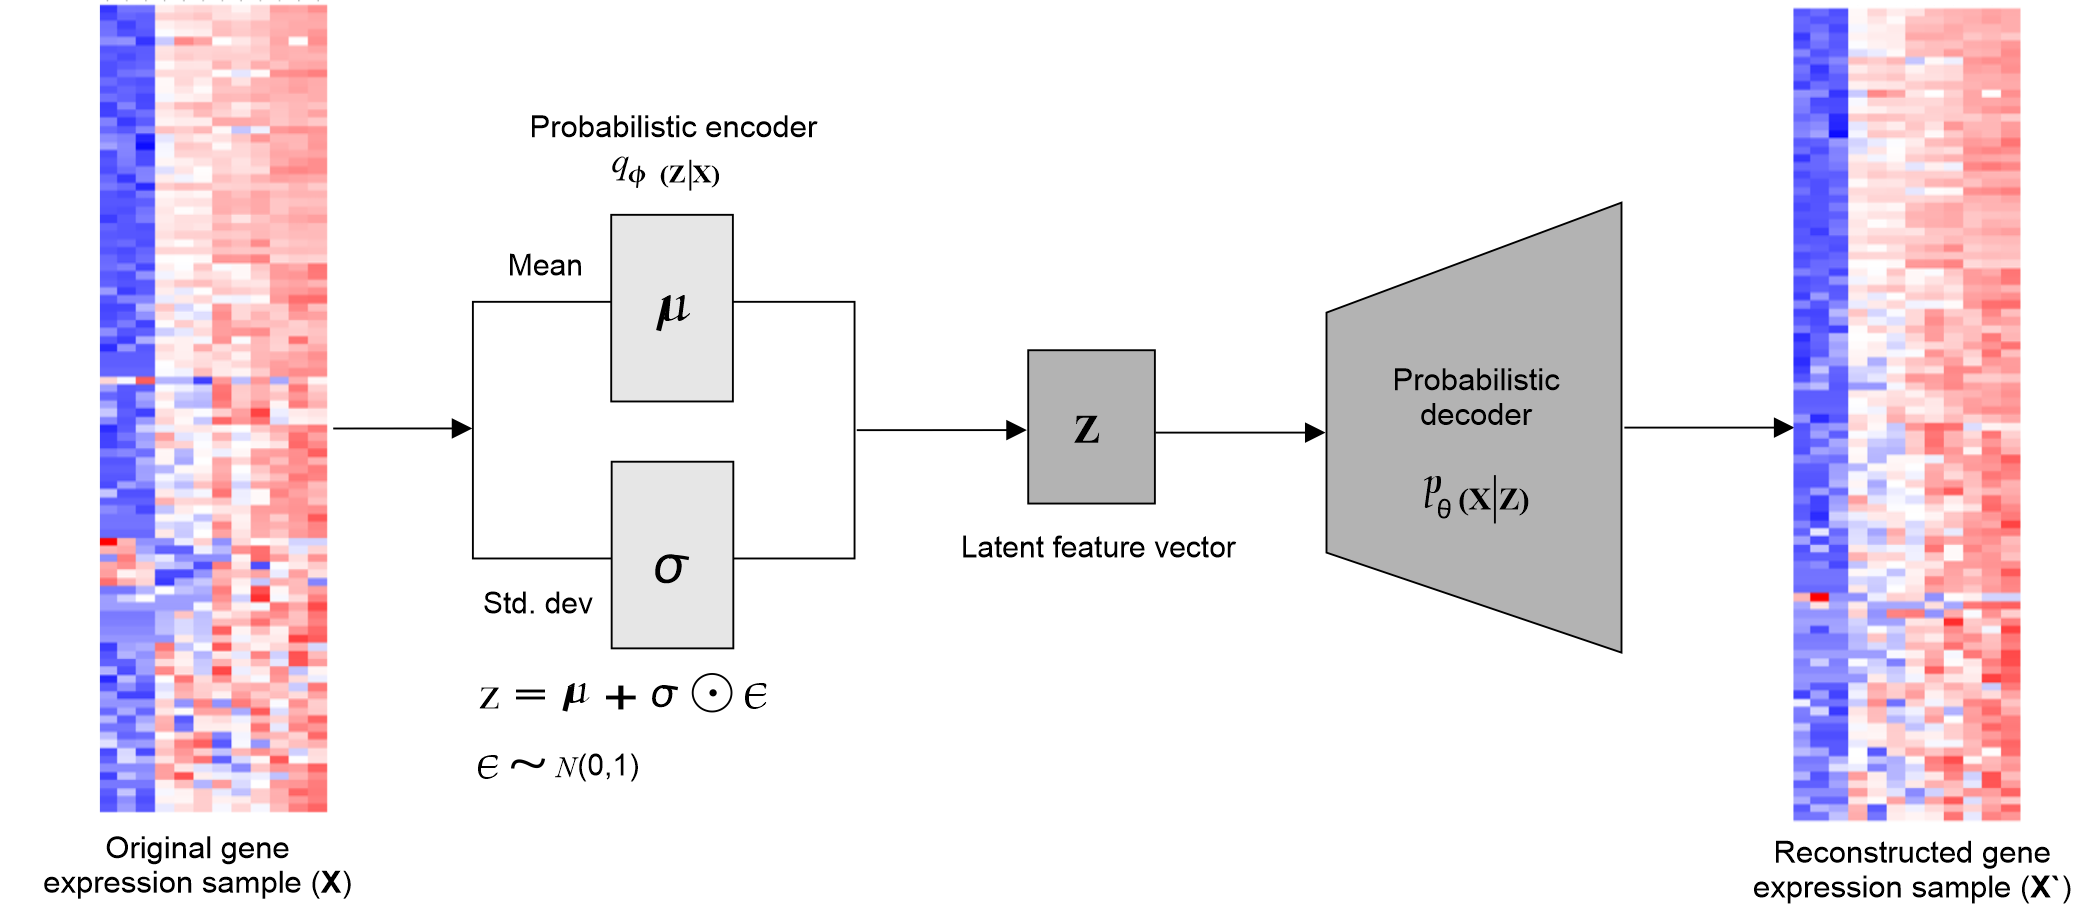
\includegraphics[width=\textwidth,height=70mm]{images/vae.png}	
	\caption{Schematic representation of a VAE used for clustering GE data, where an individual GE sample is fed into the model for learning representation~\cite{karimBIB2019}.}	
	\label{fig:vae}
	\vspace{-4mm} 
\end{figure*}

\hspace*{3.5mm} To generate a sample similar to a real data point $\mathbf{x}^{(i)}$: i) first, $\mathbf{z}^{(i)}$ can be sampled from a prior distribution $p_{\theta^{*}}(\mathbf{z})$, ii) then,  $\mathbf{x}^{(i)}$ can be generated from the conditional distribution $p_{\theta^{*}}\left(\mathbf{x} | \mathbf{z}=\mathbf{z}^{(i)}\right)$, $\theta^{*}$ is the optimal parameter that maximizes the probability of generating real data samples~\cite{VADE}:

\begin{equation}
    \theta^{*}=\arg \max _{\theta} \sum_{i=1}^{n} \log p_{\theta}\left(\mathbf{x}^{(i)}\right).
\end{equation}

\begin{equation}
    p_{\theta}\left(\mathbf{x}^{(i)}\right)=\int p_{\theta}\left(\mathbf{x}^{(i)} | \mathbf{z}\right) p_{\theta}(\mathbf{z}) d \mathbf{z}.
    \label{eq:data}
\end{equation}

\hspace*{3.5mm} The data generation process involving the encoding vector can be expressed in \cref{eq:data}~\cite{VADE}. Eventually, VAE consists of a probabilistic encoder as an approximation function $q_{\theta}(\mathbf{z} | \mathbf{x})$~(which is similar to $g_{\phi}(\mathbf{z} | \mathbf{x})$) and a generative probabilistic decoder as the conditional probability $p_{\theta}(\mathbf{x}|\mathbf{z})$~(which is similar to the decoder $f_{\theta}(\mathbf{x}|\mathbf{z})$). In variational inference, objective is to maximize the variational evidence lower bound (ELBO) by maximizing the lower bound (based on the fact that KL divergence is always non-negative, hence $-L_{vae}$ is the lower bound of $\log p_{\theta}(\mathbf{x})$) as follows~\cite{VADE}: 

\begin{equation}
    -L_{vae}=\log p_{\theta}(\mathbf{x})-L_{\mathrm{KLD}}\left(q_{\phi}(\mathbf{z}|\mathbf{x}) \| p_{\theta}(\mathbf{z}|\mathbf{x})\right) \leq \log p_{\theta}(\mathbf{x}). 
    \label{eq:lvae}
\end{equation}

\hspace*{3.5mm} VAE and its variants like LSTM-VAE~\cite{park2018multimodal}) are widely used across use cases,e.g., anomaly detection in which anomalous or outliers can be identified based on the reconstruction probability~(RP)~\cite{an2015variational}. RP is a probabilistic measure that takes into account the variability of the distribution of variables as: i) it has a theoretical background, and ii) more principled and objective anomaly score than the reconstruction loss. 

\subsubsection{LSTM-AE}
VAE or CAE are not the best options for handling sequence or time-series data, e.g., length of the input sequence in case of text clustering may vary while the network requires fixed-length inputs. Further, the temporal ordering of the observations makes the feature extraction difficult. Hence, regular AEs will fail to generate a sample sequence for a given input distribution in generative mode, whereas LSTM-AE can handle variable lengths as the encoder learns fixed-length vector representation of the input~\cite{KarimNCCA2019,karim2019drug}. Given $X$ = $\{\mathbf{x}^{(1)},\mathbf{x}^{(2)}, ..., \mathbf{L}^{(1)}\}$ a input sequence, $\mathbf{h}_E^{(i)} \in {R}^c$ is encoder's hidden state at time $t_i$ for each $i \in \{1,2,...,L\}$, and $c$ is the number of LSTM units~\cite{LSTM_Autoencoder}. The encoder and decoder are jointly trained to reconstruct the original vector in reverse order by minimizing the following objective~\cite{zhu2018hidden}:  

\begin{figure*}[h]
	\centering
	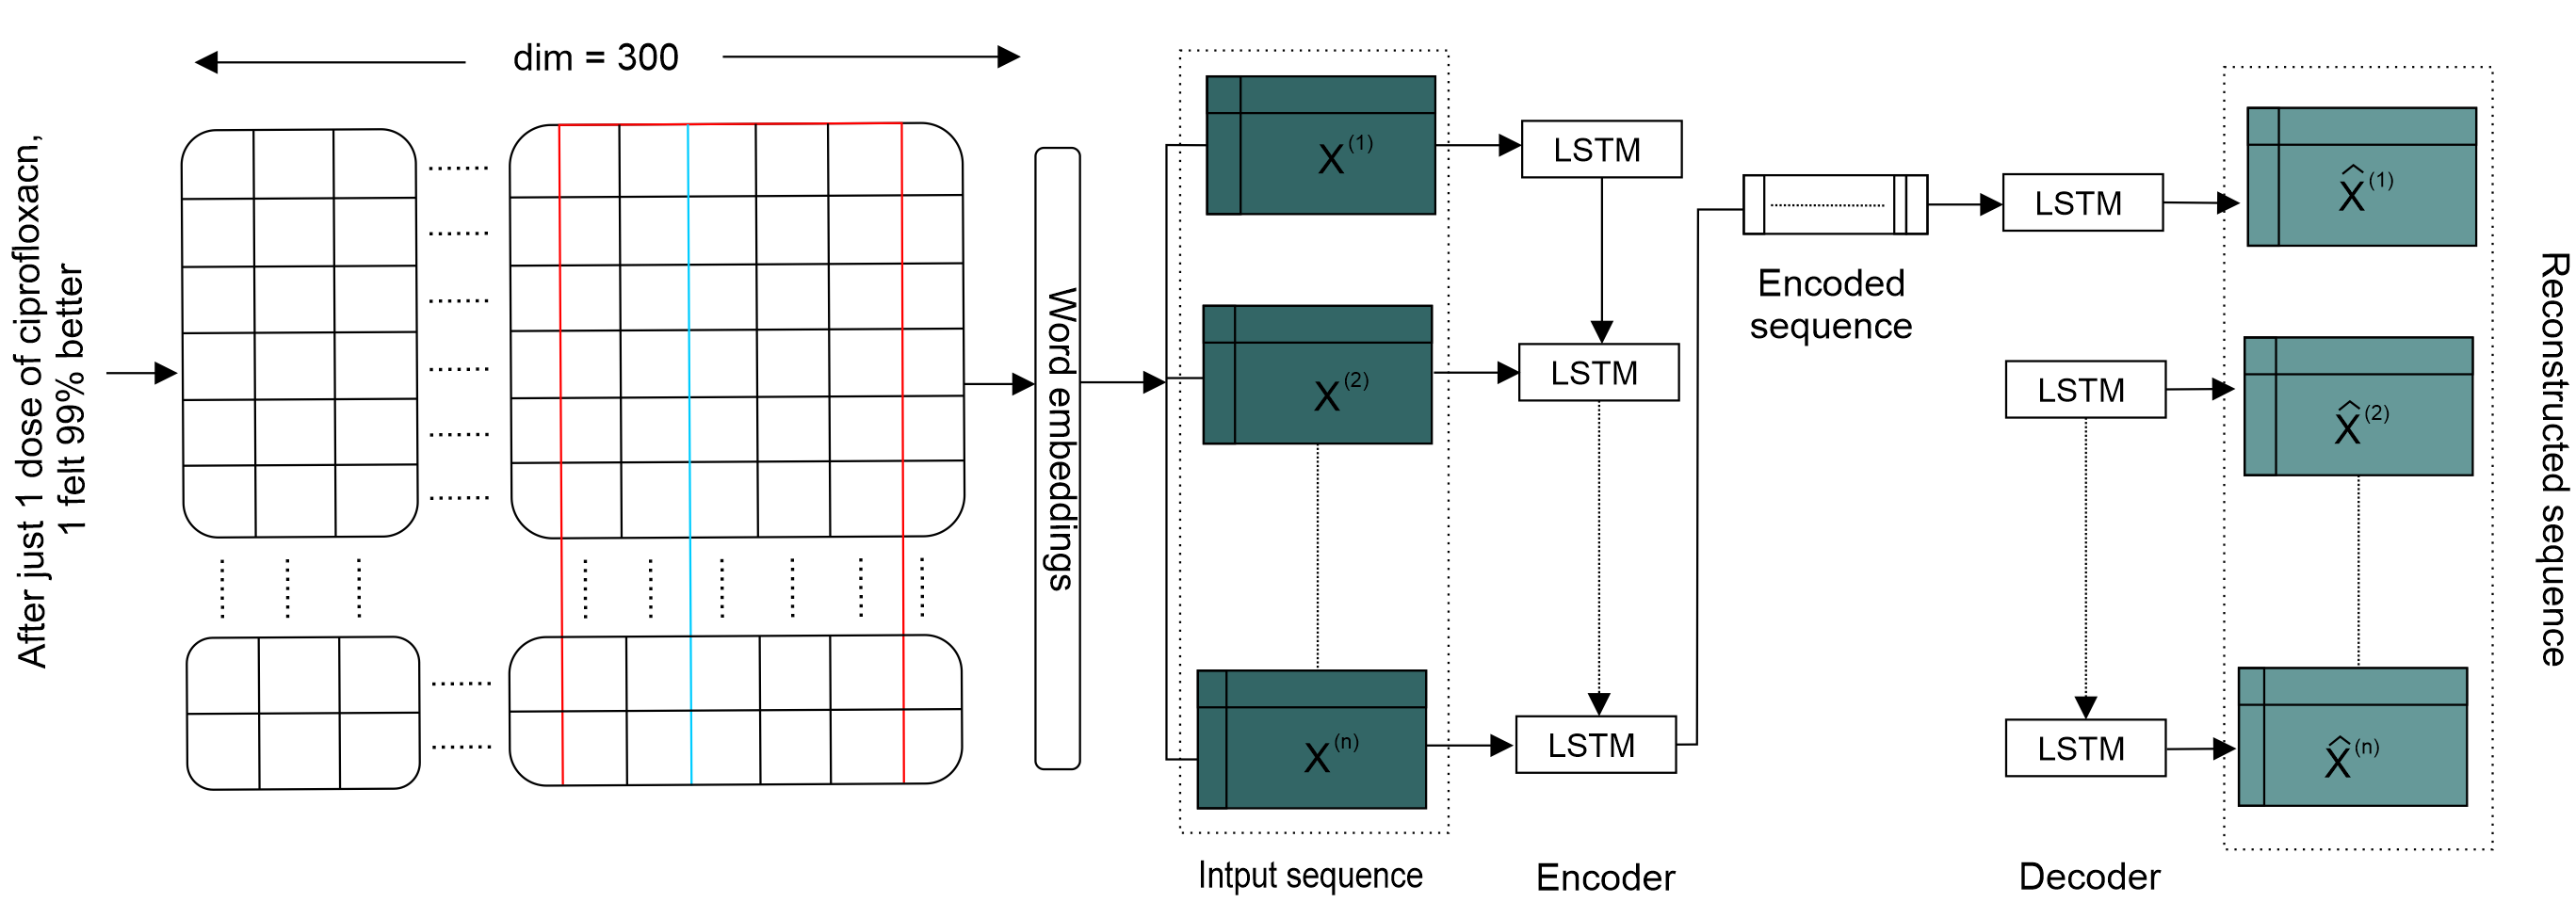
\includegraphics[width=\textwidth,height=70mm]{images/lstm_ae_v2.PNG}
    \caption{Schematic representation of the LSTM-AE, used for biomedical text clustering, where individual drug review texts are embedded using word2vec before feeding as a sequence~\cite{karimBIB2019}}	
	\label{fig:lstm_ae}
	\vspace{-2mm} 
\end{figure*}

\begin{equation}
    \sum_{X \in S_n}\sum_{i=1}^{L}\|\mathbf{x}^{(i)}-\mathbf{x}'^{(i)}\|^2
    \label{eq:obj}
\end{equation}

\hspace*{3.5mm} where $S_n$ is set of training sequences. The final state $\mathbf{h}_E^{(L)}$ of the encoder is used as the initial state for the decoder. The decoder uses $\mathbf{x}^{(i)}$ as input to obtain state $\mathbf{h}_D^{(i-1)}$ and predict $\mathbf{x'}^{(i-1)}$ corresponding to target $\mathbf{x}^{(i-1)}$~\cite{LSTM_Autoencoder} as shown in \cref{fig:lstm_ae}.  

\subsubsection{Adversarial autoencoders} 
In more recent approaches, adversarial autoencoders~(AAE) is employed in which the adversarial training procedure is followed to match the aggregated posterior of the latent representation with the prior distribution. AAE can be used to generate artificial samples with a limited number of labeled or unlabeled~(i.e., numeric or genomic) data, where the flexible nature of GAN can be utilized to extract discrete and continuous LF from large-scale data~\cite{min2018survey}. In particular, information maximizing generative adversarial network~(aka. InfoGAN)~\cite{chen2016infogan} is used for optimizing the mutual information between a fixed small subset of the GAN's noise variables and the observation~\cite{mcdaid2011normalized}, assuming: i) computation complexity is not a prime concern, ii) appropriate hyperparameters can be found. 

%\paragraph{\textbf{Sparse AE:}}  Besides, restrictions can be imposed to enforce the encoder to extract most salient features, e.g., sparsity constraint to obtain a sparse representation~\cite{min2018survey}. 
\iffalse
\subsubsection{Stacked autoencoders} 
The input can be denoised and passed through by stacking autoencoders~(SAE), e.g., where the input corruption is used only for the initial denoising. Once the mapping function $f_{\theta}$ is learned, the uncorrupted input from the previous layers are reused in the subsequent layers, e.g., then the weights of the network can be initialized with SDAE, where each layer is a DAE trained to reconstruct previous layer's output after random corruption~(i.e., DAE). SDAE can be considered a 2-layer network formulated as follows~\cite{xie2016unsupervised}:

\vspace{-6mm}
\begin{align}
    \begin{aligned}
        \tilde{x} & \sim d \text {ropout }(x) \\
        h &=g_{1}\left(W_{1} \tilde{x}+b_{1}\right) \\
        \tilde{h} & \sim d r o p o u t(h) \\
        y=& g_{2}\left(W_{2} \tilde{h}+b_{2}\right)
    \end{aligned}
\end{align}

\noindent where $dropout(.)$ is the dropout operation~\cite{srivastava2014dropout}, $g_1$ and $g_2$ are activation functions for encoding and decoding layer respectively, and $\theta$=$\lbrace{W_1, b_1, W_2, b_2}\rbrace$ are model hyperparameters~\cite{xie2016unsupervised}. Then greedy layer-wise training~(GLW) is performed by minimizing the least-squares loss $||x-y||^{2}_{2}$, i.e., after training one layer, output $h$ is used as the input to the next layer and so on. In such a scenario, ReLU activation function is used in all encoder and decoder pairs, except for $g_2$~(first pair) and $g_1$~(last pair). Once the GLW training is finished, all the encoder and decoder layers are concatenated in reverse layer-wise training order, by forming a deep AE and fine-tuned to minimize the reconstruction loss. During the GLW pre-training, each layer is pretrained for a relatively higher number of iterations with a dropout. The result is a multilayer deep AE with a bottleneck-coding layer in the middle. Based on a similar principle, other types of AE can be stacked to form such a deep AE architecture. 
\fi 

\subsection{Learning representation from multimodal data}
A multimodal representation is a representation of data using information from multiple entities~\cite{mmsurvey}. If the decision support~(or recommendation) provided by a decision support system relies on different types of input, such dataset can be characterized as multimodal. The ability to represent multimodal data in an efficient way forms the backbone of any predictive model. However, how to combine different types of data from heterogeneous sources, how to deal with different levels of noise and artifacts, and how to deal with missing data are few challenges in the multimodal RL. 

\iffalse
\vspace{-2mm}
\begin{tcolorbox}[colback=white!3!white,colframe=gray!120!black,title=\faBook~Input modality]
    %INFO: \faBook \\
    \scriptsize{
        \textbf{Input modality:} a decision support systems, which provides decision (e.g., clinical) relies on different types of data and in terms of dataset is characterized as multimodal. The term `modality' refers to the way in which we experience a real-life events that includes multiple such modalities~\cite{mmsurvey}.
        }
\end{tcolorbox}
\fi 

\begin{figure*}[htp!]
	\centering
	\begin{subfigure}{.48\linewidth}
		\centering
		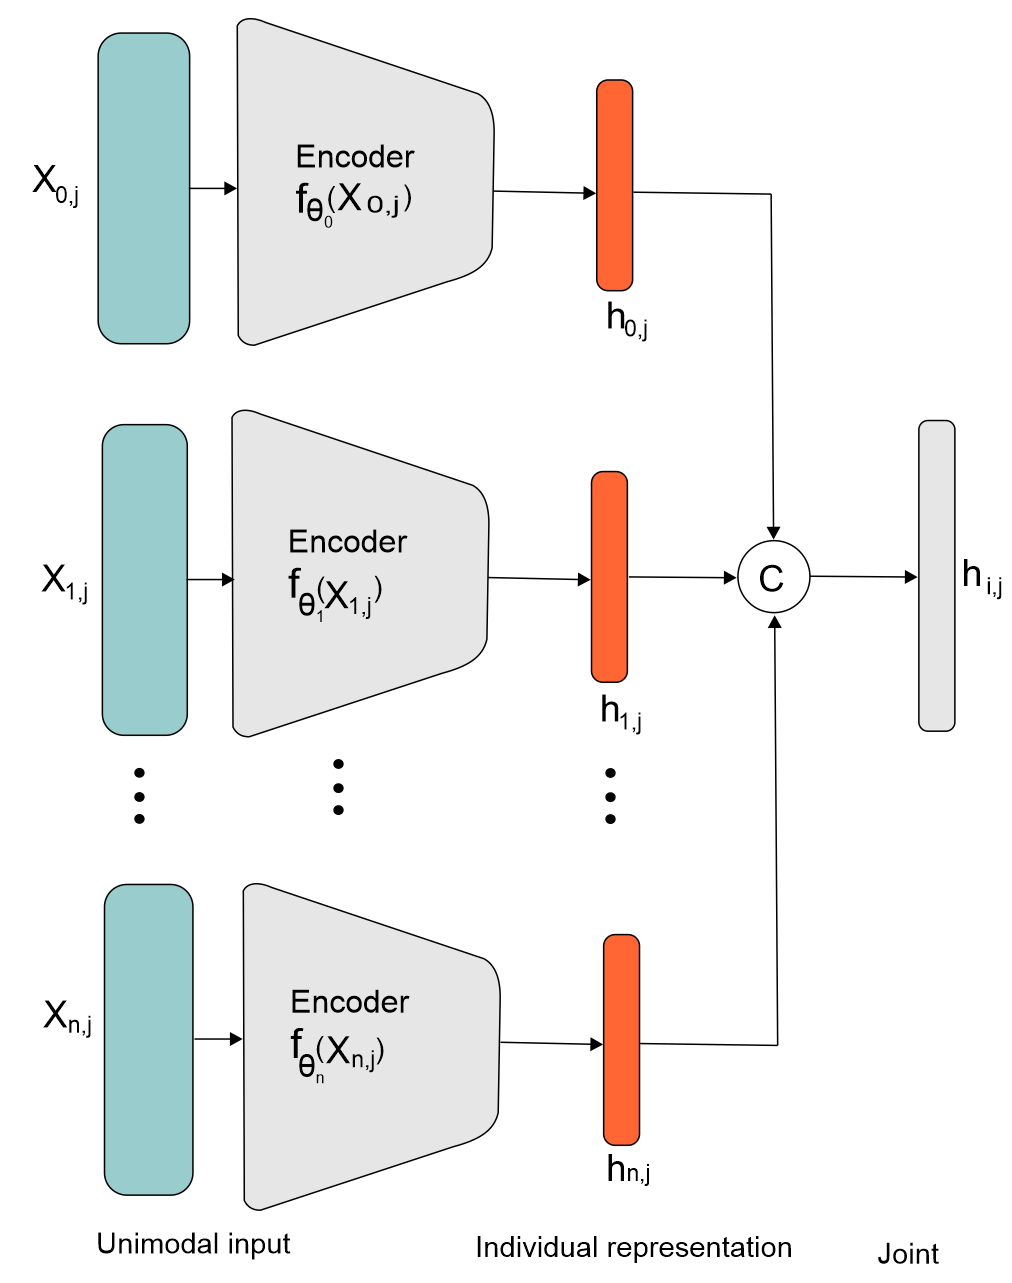
\includegraphics[width=0.95\linewidth,height=70mm]{images/rl_1.png}
		\caption{Latent representation concatenation}
        \label{fig:lrc_1}
	\end{subfigure}
	\begin{subfigure}{0.48\linewidth}
		\centering
		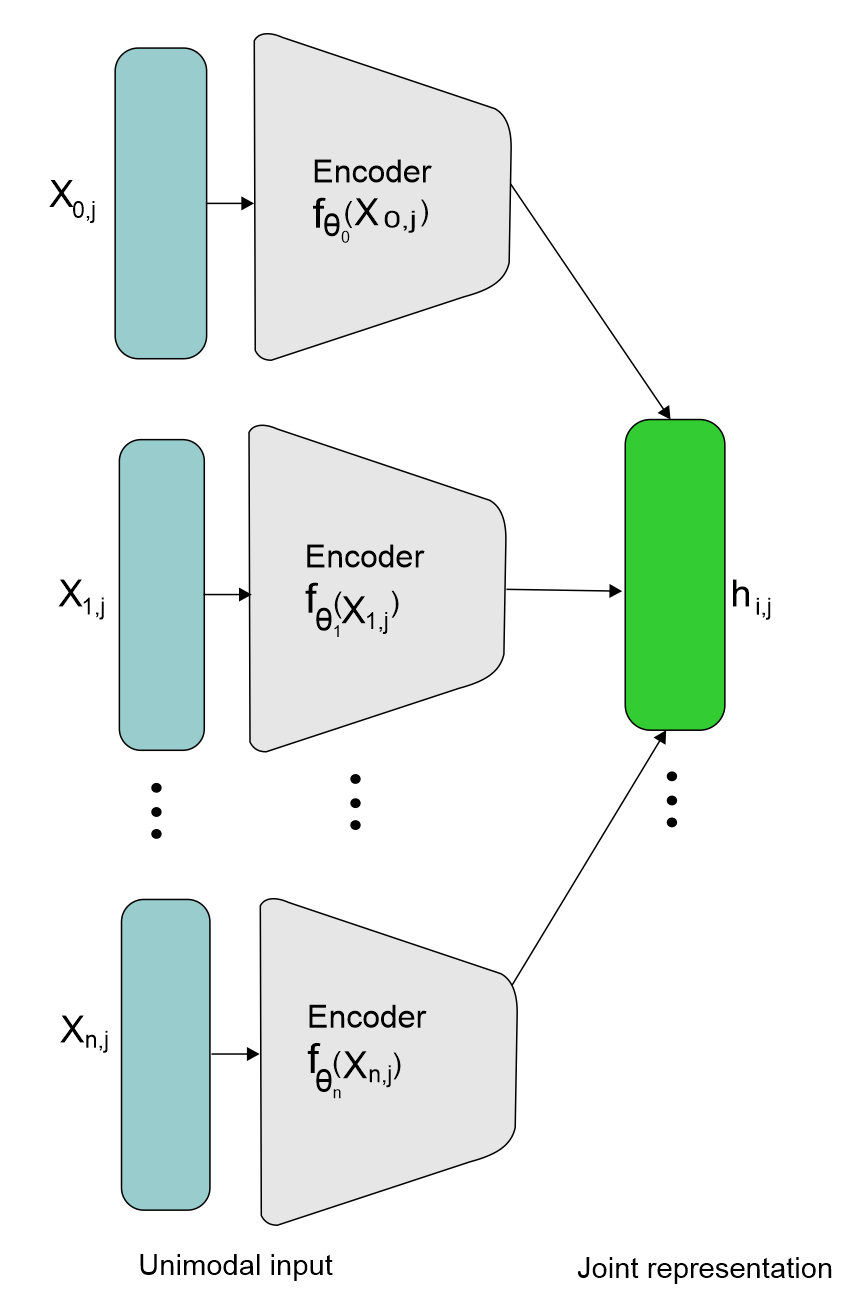
\includegraphics[width=0.95\linewidth,height=70mm]{images/shared.png}
		\caption{Shared latent representation}
        \label{fig:slr_1}
	\end{subfigure}
	\caption{Fusion architectures in multimodal representation learning (only encoder module is shown)} 
	\label{fig:mm_rL_example}
\end{figure*}

\hspace*{3.5mm} To develop a DSS, we might need to feed one~(\textit{unimodal}) or multiple types of data~(i.e., \textit{multimodal}) such as genomics, proteomics, or imaging data into the neural networks. Although several works have focused on unimodal RL, recent approaches are more focused on multimodal representations from different types of data involving simple or shared concatenation of unimodal ones~\cite{mmsurvey}. \Cref{fig:mm_rL_example} shows two fusion architectures in multimodal RL. The latent representation concatenation architecture is depicted in \cref{fig:lrc_1} consists of learning simultaneously a single latent representation from each modality. In the subsequent chapters, we'll show how to use the concatenation of all the modality-specific latent representations to train a classifier. 

\begin{figure*}[htp!]
	\centering
	\begin{subfigure}{.48\linewidth}
		\centering
		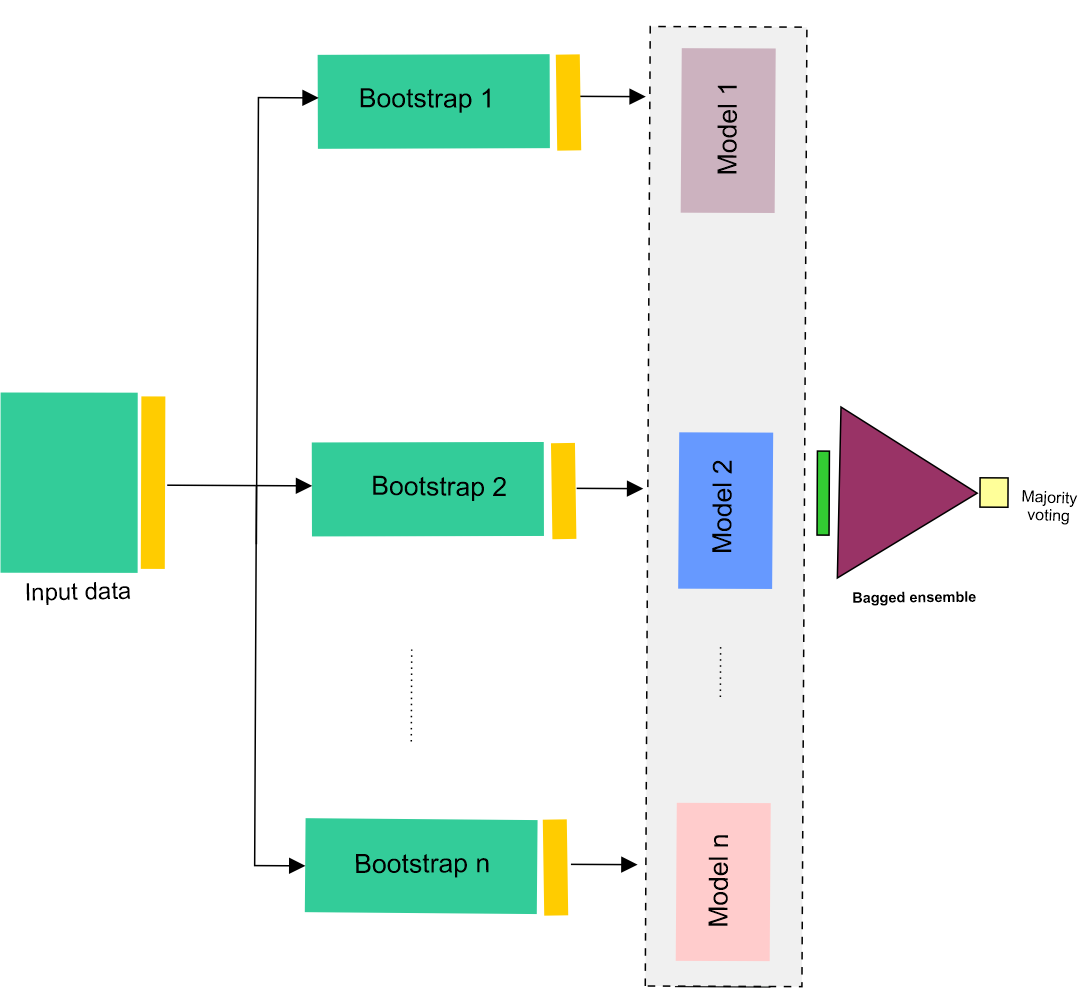
\includegraphics[width=\linewidth,height=65mm]{images/bagging.png}
		\caption{Bagging}
        \label{fig:bagging}
	\end{subfigure}
	\hspace{2mm}
	\begin{subfigure}{0.48\linewidth}
		\centering
		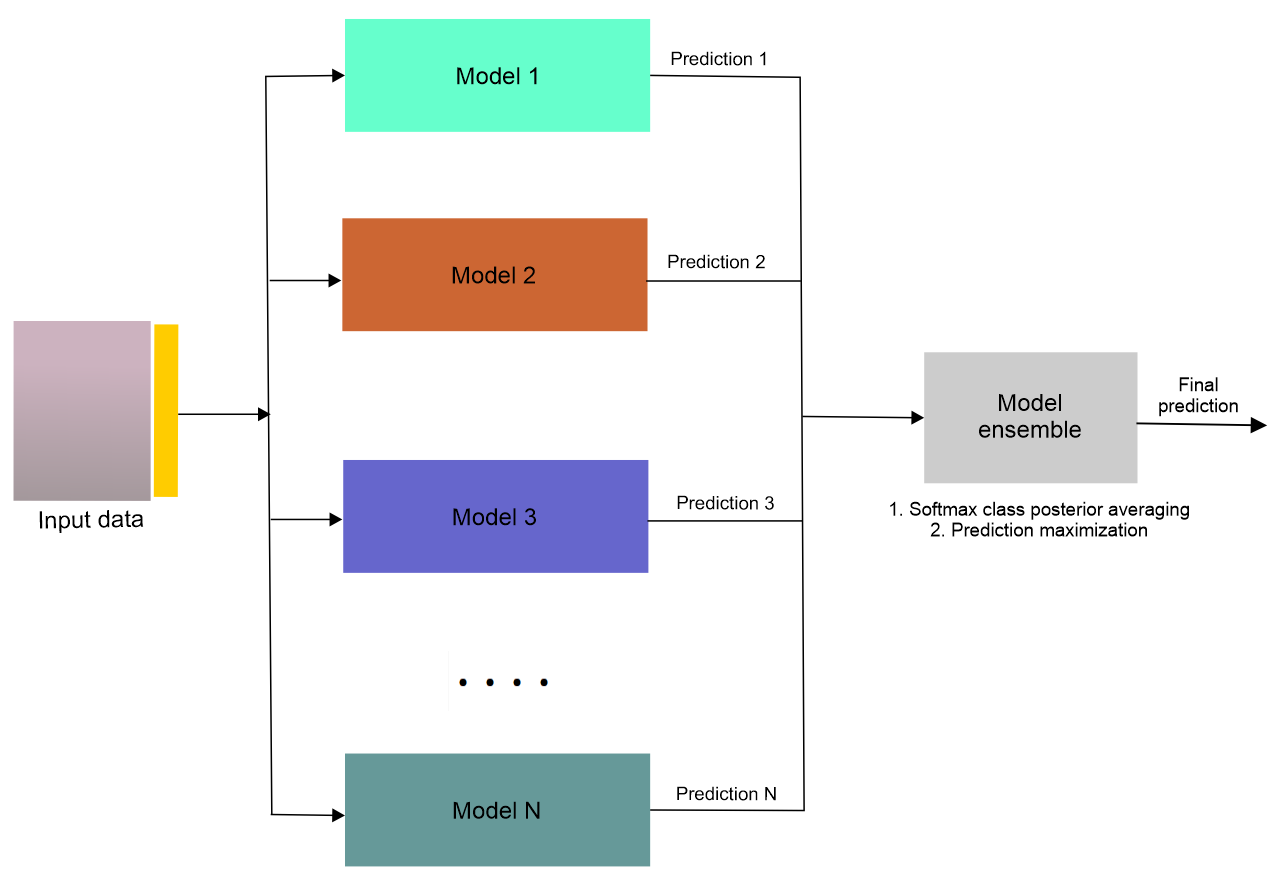
\includegraphics[width=\linewidth,height=65mm]{images/stacking.png}
		\caption{Stacking}
        \label{fig:stacking}
	\end{subfigure}
	\caption{Bagging vs. stacking: a) each model is individually trained and the predictions are voted upon, b) multiple weak learners are summed upon} 
	\label{fig:bagging_and_stacking}
	\vspace{-2mm}
\end{figure*}

\section{Model Ensemble Methods}
The ensemble modelling is based on a principle in which weak learners is grouped together to form one strong learner. First, multiple models are trained, each with the objective to predict or classify a set of results. By using ensemble methods, the stability of the final model can be increased by reducing the errors. In particular, by combining many models, mostly the variance error can be reduced. For example, by maximum voting from a panel of independent radiologists, we get the final prediction fair and trustworthy than a single radiologist. 
Model ensembling helps to achieve improved performance of a model compared to the predictions from a single model by reducing the generalization error~\cite{karimACCA2019}. Bagging, boosting, and stacking are three widely used concepts in ensembling learning to improve the classification accuracy by reducing model variance, noise, and bias: 

\begin{itemize}[noitemsep]
    \item \textbf{Bagging} is about bootstrapping and aggregating the scores over many samples. It is an effective method in case of limited labelled data. In a limited labelled data setting, smaller training set is generated by re-sampling the original training set having the sample cardinality. Bootstrapping reduces the probability of overfitting, which decreases the variance in the ensemble model. 
    \item \textbf{Boosting} is adding additional models to the ensemble model sequentially to decrease model’s bias.
    \item \textbf{Stacking} is a an ensemble method in which a new model is trained from the combined predictions of two or more previously trained models, where predictions from the previously trained models are used as inputs for each sequential layer, and combined to form a new set of predictions. Stacking helps to increase the predictive power of the final model. 
\end{itemize}

\hspace*{3.5mm} When it comes to neural ensemble, it can be achieved by training multiple model snapshots during a single training of a neural network and combining their predictions to make an ensemble prediction called snapshot ensemble~\cite{huang2017snapshot}. A limitation of this approach, however, might be that the saved models will be similar, resulting in similar predictions and predictions errors. Hence, we cannot expect much benefit from combining their predictions unless we have already introduced diversities during model training~\cite{huang2017snapshot}. This issue is addressed in \cref{chapter:uni_modality}, by changing the learning algorithm to force the exploration of different network weights during a single training run that will result slightly different performance\cite{karimACCA2019}. 

\section{Hyperparamters Tuning}
ML models are composed of two different types of parameters called model parameters and hyperparameters. While the former parameters are learned during the model training such as weights in neural networks, the latter parameters can be arbitrarily set by the user before starting training like number of estimators in random forest or learning rate in a neural network. In other words, model parameters are learned during the training, while hyperparameters are set by the human, e.g., data scientist before the training.

\hspace*{3.5mm} Often parameters that define model architecture are called hyperparameters, where the prefix `hyper refers that it is not a `model parameter', i.e., can be optimized during the training. More technically, model parameters are learned during the training while we optimize a loss function using an optimizer such as RMSProp, whereas hyperparameters are not model parameters and cannot be directly trained from the data. Following are a few examples of hyperparameters: 

\vspace{-1mm}
\begin{itemize}[noitemsep]
    \item \textbf{Linear model} - degree of polynomial features.
    \item \textbf{Clustering} - number of clusters~(i.e., k) in a k-means clustering.
    \item \textbf{Tree and tree-ensemble} - maximum depth of the decision tree~(DT), the minimum number of samples at a leaf node in the DT, number of trees to include in a random forest model. 
    \item \textbf{Neural networks} - number of neurons in a hidden layer, number of layers, learning rate for stochastic gradient descent for backpropagation. 
\end{itemize} 
\vspace{-2mm}

\iffalse
\begin{tcolorbox}[colback=white!3!white,colframe=gray!120!black,title=\faBook~Random vs. grid search for hyperparameter optimization]
    \scriptsize{
        \textbf{Grid search:} in the following figure, $x$ number of values are picked, which are evenly spaced along each axis, forming a grid. Then a model is trained for each possible combination, followed by evaluating each model, and selecting the architecture giving the best result. \\
        }
    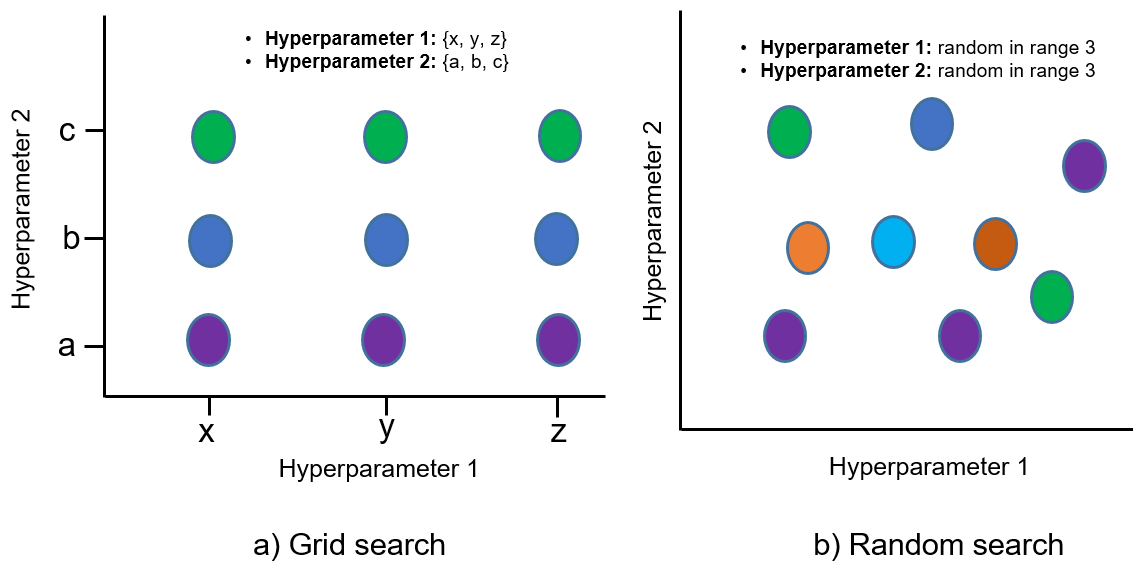
\includegraphics[width=0.8\textwidth]{images/gvr.png}\\ 
    \scriptsize{
        \textbf{Random search:} $x$-squared number of values are picked randomly and used in cross validation to test the accuracy of the experiment for each combination.
        } 
\end{tcolorbox}
\fi 

\subsection{Techniques for hyperparameter optimization}
Since an appropriate selection of hyperparameters have huge impact on the performance of ML model, `hyperparameter tuning' is performed, which is the process of searching best model based on optimal combination of hyperparameters. In other words, hyperparameter optimization~(HPO) is the problem of choosing the best combination~(or optimal) hyperparameters for a learning algorithm. HPO is often represented as the following objective function: 

\vspace{-6mm}
\begin{align}
    x^{\star}=\arg \min _{x \in \mathcal{X}} f(x)
    \label{eq:hpt}
\end{align}

\hspace*{3.5mm} where $x \in X$, $f(x)$ represents an objective score to minimize, e.g. RMSE evaluated on the validation set and $x^*$ is the set of hyperparameters to yield the lowest value of the score. However, in case of complex model, there are more than one hyperparameter on which there are several approaches to perform hyperparameter tuning such as grid search, random search, and Bayesian optimization. 

\begin{figure*}[h]
	\centering
	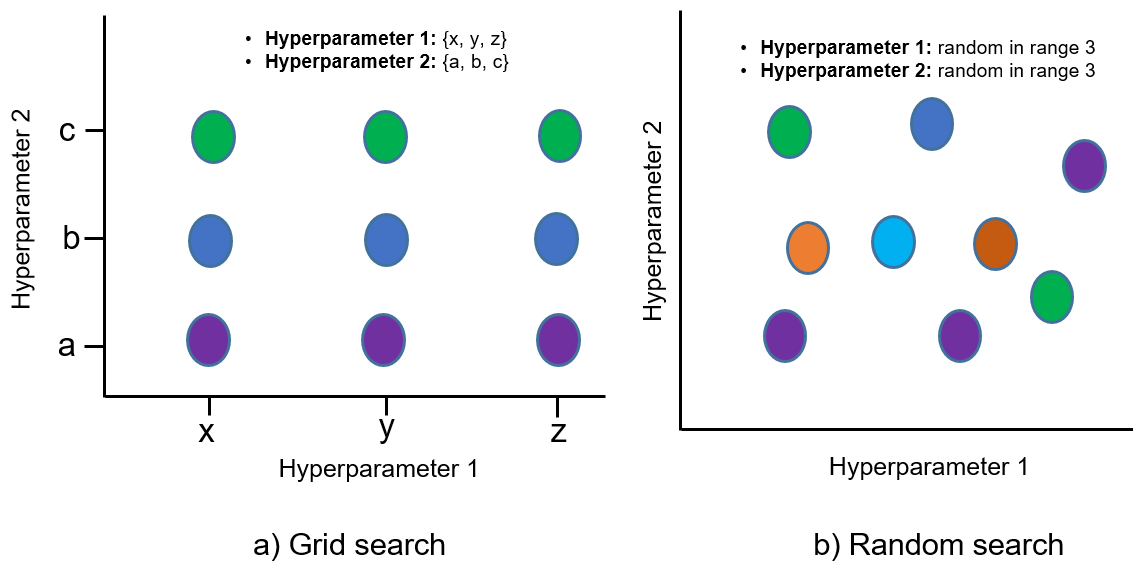
\includegraphics[width=0.8\textwidth,height=50mm]{images/gvr.png}
    \caption{Random vs. grid search for hyperparameter optimization}	
	\label{fig:random_vs_grid_search}
	\vspace{-2mm} 
\end{figure*}

\subsection{Grid search and random search}
In grid search, evenly spaced values are generated for each hyperparameter being tested, followed by building a model for each possible combination of all of the hyperparameter values, evaluating each model and selecting the architecture which produces the best results. %\subsection{Random search}
In random search, random values for each hyperparameter are generated that are used in cross-validation to evaluate the model for each combination.

\begin{itemize}[noitemsep]
    \item In \textbf{grid search}, $x$ number of values are picked, which are evenly spaced along each axis, forming a grid, as shown in \cref{fig:random_vs_grid_search}. Then a model is trained for each possible combination, followed by evaluating each model, and selecting the architecture giving the best result.
    \item In \textbf{random search}, $x$-squared number of values are picked randomly and used in cross validation to test the accuracy of the experiment for each combination, as shown in \cref{fig:random_vs_grid_search}.
\end{itemize}

\hspace*{3.5mm} Random search is better than grid search for most cases, hyperparameters are not equally important, making some hyperparamters are more important than others. A Gaussian process analysis of the function from hyper-parameters to validation set performance reveals that for most data sets only a few of the hyper-parameters really matter, but that different hyper-parameters are important on different data sets. This phenomenon makes grid search a poor choice for configuring algorithms for new data sets. %- Bergstra, 2012

\subsection{Bayesian optimization} 
Both grid search and random search perform individual experiments~(i.e., one model training) while training the model with various hyperparameter values and observe the performance of the model in each case. Many optimization problems in ML are black box optimization problems, where the objective function $f(x)$ in \cref{eq:hpt} is a black box function~\cite{BO}. It neither interprets the analytical expression for $f$, nor we know its derivatives. Oftentimes, evaluation of the function is restricted to sampling at a data point $x$ and getting a possibly noisy response~\cite{BO}.
Nevertheless, as each experiment using grid search and random search is performed separately, reusing the result of current experiment to improve the next one is not possible. However, they can easily be parallelized by employing an approach called ``Bayesian optimization"~(BO), which belongs to a class of sequential model-based optimization algorithms. BO allows using the results of the previous iteration to improve the sampling method of the next experiment.

\hspace*{3.5mm} BO incorporates prior belief about $f(x)$ and updates the prior with samples drawn from $f(x)$ to get a posterior that better approximates $f(x)$. The model used for approximating the objective function is called surrogate model. In BO, a model is initially defined and trained with hyperparameters $\sigma$, which is scored $v$ w.r.t some evaluation metrics\footnote{Metrics could be different depending upon task at hand}. The previously evaluated hyperparameter values are reused to compute a posterior expectation of the hyperparameter space. Optimal hyperparameter values are then chosen according to this posterior expectation as the next model candidate, which is repeated iteratively until it converges to the optimal value. While, the Gaussian process is employed to model the prior probability of model scores across the hyperparameter space,  
%This model then enables to use the hyperparameter values $\sigma_1,\sigma_2,...,\sigma_n$ and corresponding scores $v_1,v_2,...,v_n$ to approximate a continuous score function over the hyperparameter space. %It includes the degree of certainty of the estimate, which can be used to identify the candidate hyperparameter values, which hopefully would yield the largest expected improvement over the current score. 
BO finds a better optimum in a smaller number of steps than random search and beats the baseline in almost every run~\cite{BO}. Using BO in case of a clinical DSS becomes even more evident, given the fact that we have such a high-dimensional search spaces, e.g., many omics data often have 20K+ dimensionality. 

\section{Interpretability of ML Models}
Although DL models have shown tremendous success at AI-aided diagnosis and prognosis, showing high effectiveness and accuracy, there are many cases where not only high accuracy, but also explanation about the outcome is necessary. Suppose we have an accurate model that can classify cancerous samples with an accuracy of 90\%. Still, we cannot claim that it has high confidence at providing accurate and trustworthy diagnosis, given that the single accuracy metric is an incomplete description~\cite{doshi2017towards} and can't be enough in AI-aided diagnosis and prognosis, unless it explains the reason behind the  decision. Otherwise, such a model has to perceive a `black box' method as it cannot explain why it reached to such a diagnosis decision. % and lack of transparency.  
If the parameters $\boldsymbol{\theta}$ of a ML model $\boldsymbol{f}$ and it's architecture are known, the model is considered a `white-box'. %A white-box model also helps improve model-debugging and promotes trust. 
A `white-box' model is not necessarily explainable or interpretable~\cite{das2020opportunities}, while an ML model $\boldsymbol{f}$ is considered a `black-box' if the model parameters and network architectures are hidden from the end-user. We slightly tweaked the definitions of `black-box' and `white-box' models provided by Das et al.~\cite{das2020opportunities}: 

\begin{definition}
    \textbf{black-box model} - an ML model $f$ is considered `black-box' if the model parameters and network architectures are hidden from the end-users. 
\end{definition}

\begin{definition}
    \textbf{white-box model} - an ML model $f$ is `white-box' if its parameters $\boldsymbol{\theta}$ and architecture are known to the end users, by providing sufficient knowing of the working principles. % and why it provides a specific decision.  
\end{definition}

\hspace*{3.5mm} In contrast, interpretable ML refers to methods that make the behavior and predictions of a system understandable to humans~\cite{molnar2019interpretable}. 
%This is a serious drawback since interpretability is essential to generate insights on why a given cancer case is of a certain type, and since knowing the most important biomarkers can help in recommending more accurate treatments and drug repositioning. 
%Further, the `right to explanation' of the EU GDPR~\cite{kaminski2019right} gives patients the right to know why and how an algorithm made a diagnosis decision. However, existing approaches can neither ensure the diagnosis transparently nor are they trustworthy. 
%AI-aided system has to be well-interpretable and explainable.
Interpretability of an ML system is the ability to explain or to present in understandable terms to a human~\cite{doshi2017towards}. Miller et al.~\cite{XAI_miller} defines interpretability as the degree to which a human can understand the cause of a decision. Although a white-box model improves model-debugging and promotes trust, knowing it's architecture and parameters alone won't make the model essentially explainable~\cite{das2020opportunities}.  %~(\cref{def:xai_1}) and Kim et al.~\cite{XAI_kim}~(\cref{def:xai_2}), respectively:
\iffalse
\begin{definition}
    \textbf{interpretability}: is the degree to which a human can understand the cause of a decision.
    \label{def:xai_1}
\end{definition}
\vspace{-6mm}
\begin{definition}
    \textbf{interpretability}: is the degree to which a human can consistently predict model's result.
    \label{def:xai_2}
\end{definition}
\fi 
%\vspace{-6mm}
Model interpretation is an extension of the model evaluation, which helps to foster a better understanding of a model’s learned decision policies and gives the ability to explain a model in a way which is human understandable such that the outcomes are self-descriptive and needs no further explanation. 
The higher the interpretability, the easier it is for human to comprehend why a particular decision or prediction is made~\cite{stiglic2020interpretability,bhatt2020explainable}, i.e., trustworthiness for the human. In either way, good interpretability is desired both locally, e.g., individual predictions and globally, e.g., entire model behavior. 

\begin{figure*}[h]
	\centering
	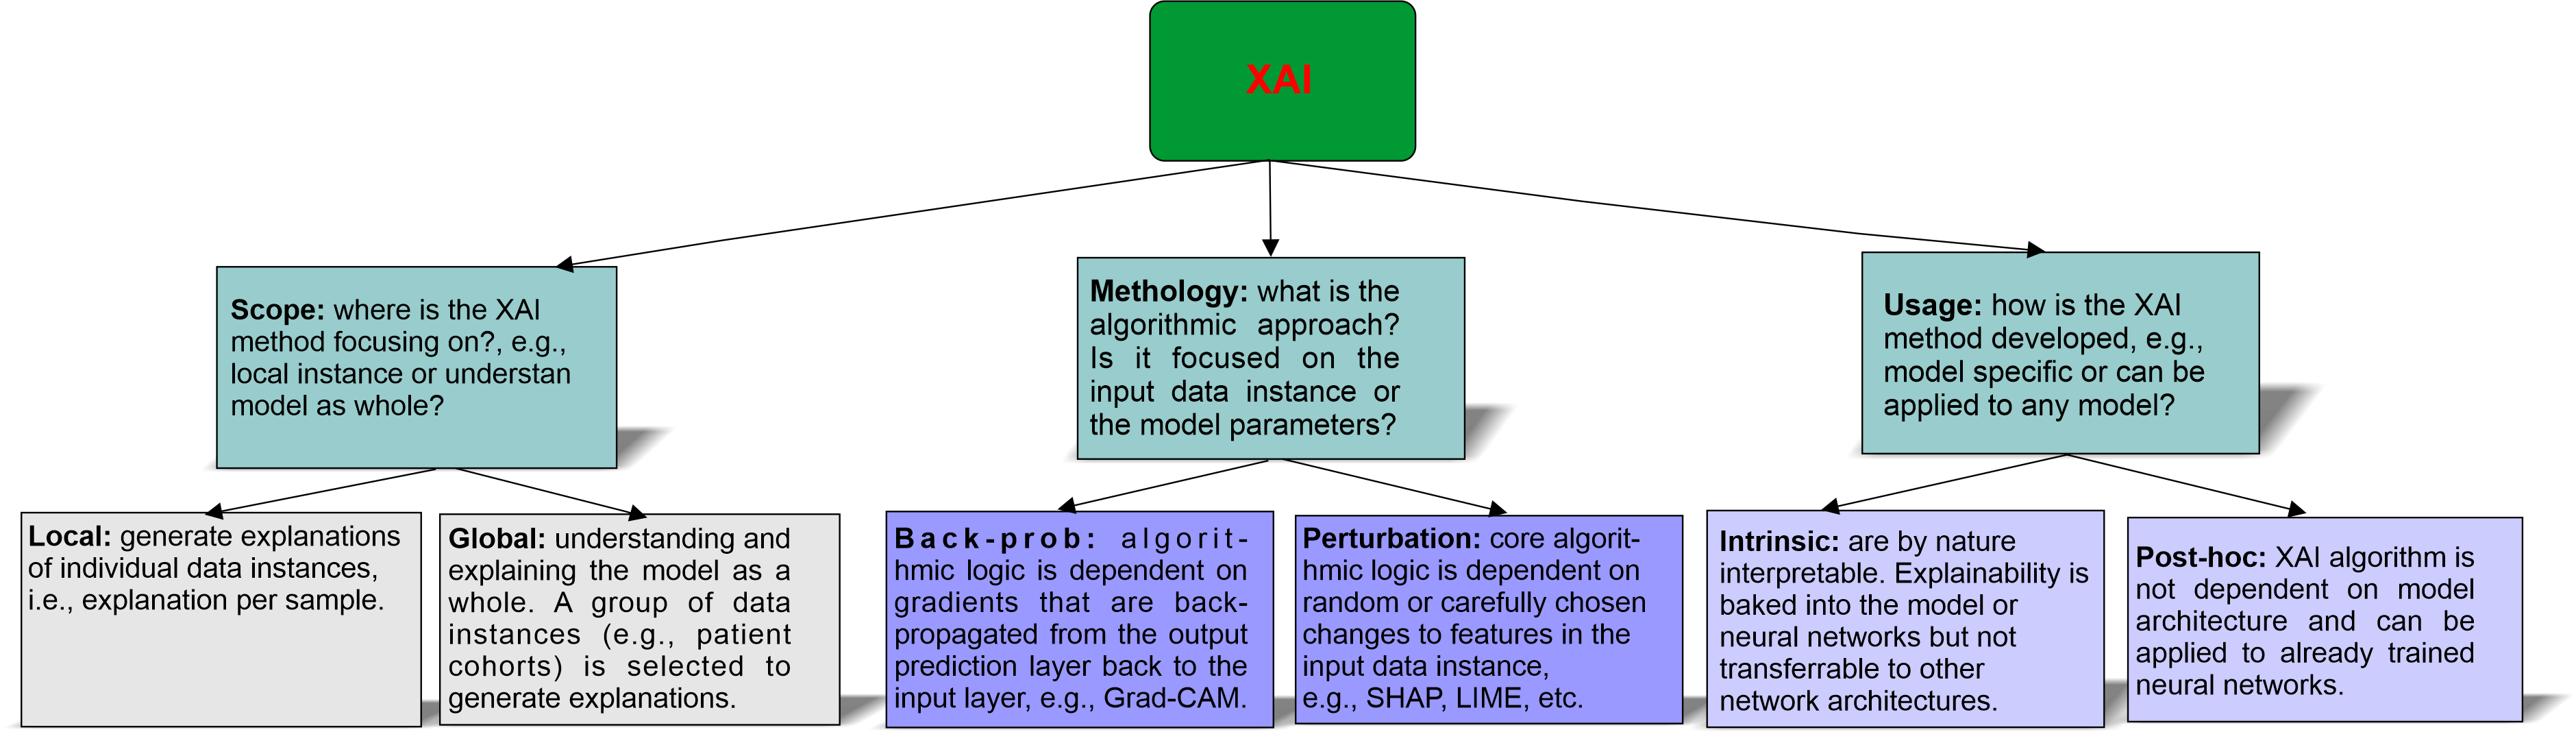
\includegraphics[width=0.9\textwidth,height=60mm]{images/xai_tec.png}	
    \caption{Categorization of the survey in terms of scope, methodology, and usage~(based on~\cite{das2020opportunities})}	
	\label{fig:survey_xai}
\end{figure*}

\hspace*{3.5mm} Although many authors used interpretability and explainability interchangeably, the former means that the cause and effect~(e.g., of a certain outcome) can be determined in a system. The latter is the extent to which the internal working mechanism of an AI system can be explained to humans, in human-interpretable language. Miller et al.~\cite{miller2018explanation} defined explanation as the answer to `why' and `how' types of questions. For example, in the cancer diagnosis context, a patient may have the following questions: i) why do I have colon cancer?, ii) Why did the treatment not work on me?, iii) how did the model predict the decision?, etc. However, there is a trade-off between explianability and accuracy. How well does an explanation predict unseen data is a measurement of accuracy~\cite{molnar2019interpretable}. High accuracy is important if the explanation is used for predictions in place of the ML model. However, if the goal is to explain what the `black-box' model does~(i.e., algorithmic transparency), only `fidelity' is important~\cite{molnar2019interpretable}. 

\subsection{Algorithmic transparency}
An ML model is considered transparent if it is expressive enough to be human understandable, where transparency can be a part of the algorithm itself or using external means~(e.g., model decomposition or simulations)~\cite{das2020opportunities}. Although the phrase `algorithmic transparency' was coined by Nicholas D. et al.~\cite{diakopoulos2017algorithmic} in 2016 w.r.t the role of algorithms in deciding the content of digital journalism, the underlying principle dates back to 1970s and the rise of automated systems for scoring consumer credit~\cite{diakopoulos2015algorithmic}.  Algorithmic transparency suggests \textit{factors that influence the decisions made by algorithms should be visible, or transparent, to the people who use, regulate, and are affected by systems that employ those algorithms}~\cite{diakopoulos2017algorithmic}.  %\footnote{\url{https://en.wikipedia.org/wiki/Algorithmic_transparency}}. 

\iffalse
\begin{definition}
    {\textbf{algorithmic transparency}} is the principle that the factors that influence the decisions made by algorithms should be visible, or transparent, to the people who use, regulate, and are affected by systems that employ those algorithms.
\end{definition}
\fi 

\hspace*{3.5mm}More technically, ``algorithmic transparency" is how the algorithm learns a model from the data and maps different relationships transparently based on what prediction it makes for unknown samples. First example could be a decision tree algorithm, which implicitly performs variable screening or feature selection. Hence, feature importance is clear, showing clear interactions between features. The second example could be image classification using neural networks, e.g., while classifying images, a CNN model learns features~(e.g., class-discriminating pixels) using edge detectors and filters across convolutional layers. Subsequently, it can learn more abstract features in the deepest layer to provide attention on some areas using attention maps, explaining where most important pixels are located.

\iffalse
\vspace{-2mm}
\begin{tcolorbox}[colback=white!3!white,colframe=gray!120!black,title=\faBook~Algorithmic transparency]
    %INFO: \faBook \\
    \scriptsize{
        \textbf{Algorithmic transparency:} is how a learning algorithm learns a model from the data by mapping relations to make prediction for unknown sample.
        }
\end{tcolorbox}
\fi 

\hspace*{3.5mm} 
%Less technically, Algorithmic transparency is how a learning algorithm learns a model from the data by mapping relations to make prediction for unknown sample. 
There are a several ways to transparently show how a learning algorithm works. Some models are inherently interpretable, some are not. For example, DNNs that are propagating gradients through a network with millions of weights are less understood because of their inner workings, are less transparent~\cite{molnar2019interpretable}. However, they way a linear~(linear or logistic regression) or tree-based model~(decision trees) learn is very transparent and is characterized by a high transparency. Algorithmic transparency requires only knowledge of the algorithm, not of the data or learned model itself~\cite{molnar2019interpretable}. Implicitly, ``algorithmic transparency" also means that the inputs used by the algorithm must be known, but they necessarily need not be fair. 

\subsection{Needs for interpretability}
Although, not all predictions made by an ML algorithm needs to be explained, interpretability is essential for end users's trust and to effectively manage the emerging generation of AI applications~\cite{das2020opportunities}. In general, ML models needs to be interpretable, higher interpretability of the model means easier comprehension and explanation of future predictions for end-users~\cite{stiglic2020interpretability}. With the wider usage of AI in numerous domains, the need to explain an ML model result is important for ethical, judicial, as well as safety reasons~\cite{das2020opportunities}. 
%Literature have discussed important aspects showing the importance of the XAI. Among others, 
Three most important concerns identified by Das et al.~\cite{das2020opportunities} are trustability, transparency, and fairness of AI algorithms. \Cref{fig:need_for_xai} depicts some critical areas where both explainability and transparency are crucial. 
%Current business models include interpretation as a step before serving the ML models on production systems, however are often limited to small tree-based models. With the use of highly nonlinear deep learning algorithms with millions of parameters in ML pipelines, XAI techniques must improve all three concerns mentioned above. 
%However, interpretability stems from an incompleteness in the problem formalization, which evolves a fundamental barrier to optimization and evaluation~\cite{doshi2017towards}. Note that incompleteness is distinct from uncertainty: the fused estimate of a missile location may be uncertain, but such uncertainty can be rigorously quantified and  formally reasoned about. In ML terms, we distinguish between cases where unknowns result in quantified variance—e.g. trying to learn from small data set or with limited sensors—and incompleteness that produces some kind of unquantified bias—e.g. the effect of including domain knowledge in a model selection process. In short, interpretability is desired and essentials in several aspects, e.g., scientific understanding and ethics.

\iffalse
\begin{figure*}[h]
	\centering
	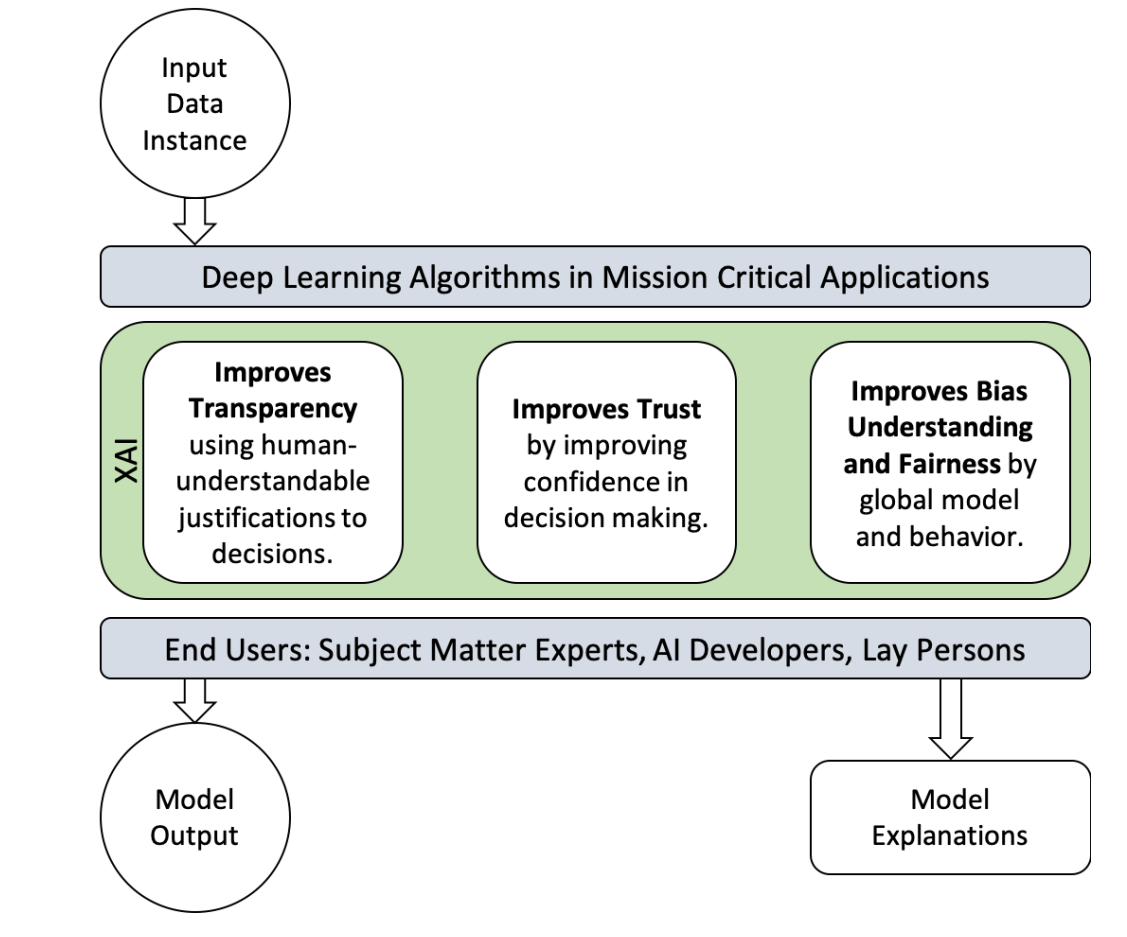
\includegraphics[width=\textwidth,height=40mm]{images/adv_xai.png}	
    \caption{Significant expected improvements when using XAI techniques to support decision making of end-users. We believe XAI is important due to improvements in trust, transparency, and in understanding bias and fairness.~(based on~\cite{das2020opportunities})}	
	\label{fig:survey_xai}
\end{figure*}
\fi 

\begin{figure*}[h]
	\centering
	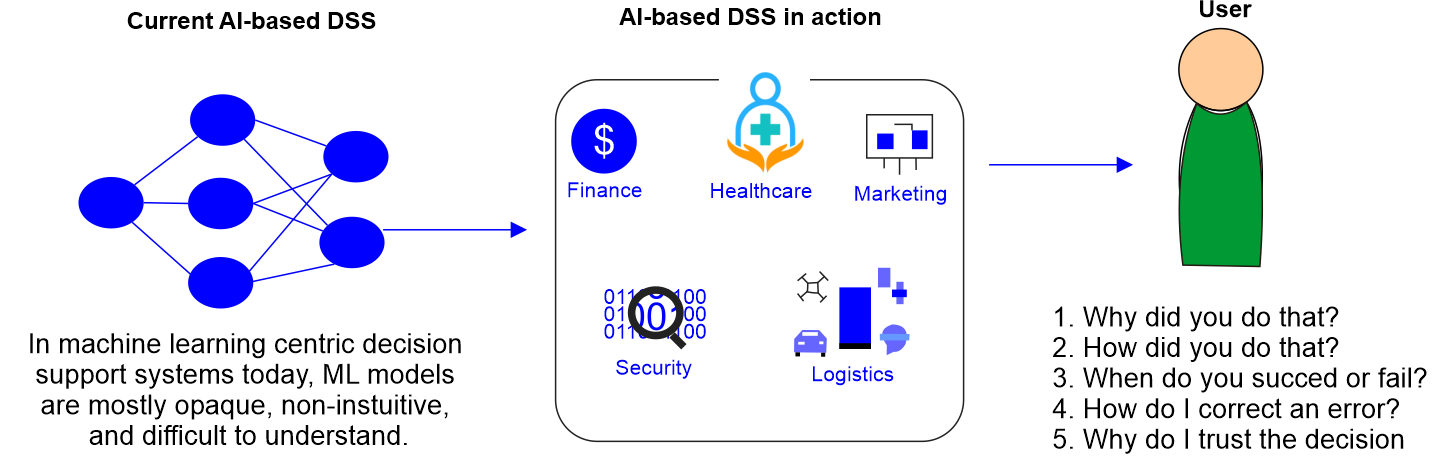
\includegraphics[width=\textwidth,height=45mm]{images/why_xai.png}	
    \caption{Needs for explainability and transparency in DSS}	
	\label{fig:need_for_xai}
\end{figure*}

%\hspace*{3.5mm} XAI techniques improve the transparency by creating a human-understandable justification to the decisions and could find and deter adversarial examples if used properly~\cite{das2020opportunities}. XAI techniques can improve trust. Trustability of an ML model is a measure of confidence in the intended working of a given model in dynamic real-world environments. Often decisions and judgements are primarily based on the knowledge and available explanations to situations and the trust we generate. 
%A scientific explanation or logical reasoning for a sub-optimal decision is better than a highly confident decision without any explanations~\cite{das2020opportunities}. XAI techniques improve fairness by mitigating different types of bias. While bias in ML realm indicate the disproportionate weight, prejudice, favor, or inclination of the learnt model towards subsets of data due to both inherent biases in human data collection and deficiencies in the learning algorithm, fairness is the quality of a learned model in providing impartial decisions without favoring any populations in the input data distribution~\cite{das2020opportunities}.
%Eventually, XAI promotes fairness and helps mitigate biases introduced to the AI decision either from input datasets or poor neural network architecture.

\hspace*{3.5mm} Further, the article 14 of the EU GDPR~\cite{kaminski2019right} states that when a company uses automated decision-making tools, it must provide ``meaningful information about the logic involved, as well as the significance and the envisaged consequences of such processing for the data subject”~\cite{kaminski2019right}. In the same time, GDPR prohibits the use of ML for automated decisions unless a clear explanation of the logic used to make each decision is well-explained, which is not possible with conventional ML; mainly, due to the black-box nature. In case of ML-based profiling and automated decisions, following requirements have to be ensured~\cite{doshi2017towards}: 

\begin{enumerate}[noitemsep]
    \item Ability to identify processes involved in the business.
    \item Monitoring the ML model being currently used.
    \item Assessing the deployed model against the interpretability and prediction biases. 
    \item Assessing the ability of the model for generating human-interpretable decision rules. 
    \item Developing a strategy for meeting compliance requirements in each stage of the ML workflow.  
\end{enumerate}

\subsection{Scopes and implementation levels for interpretability}
\Cref{fig:survey_xai} shows the categorization of the survey in terms of scope, methodology, and usage. As shown, a wide range of strategies for interpretable ML have been developed and applied to numerous areas, ranging from model-agnostic to model-specific. They are often characterized based on if they provide global or local interpretations~\cite{azodi2020opening}. Depending on the abstraction, two types of interpretability called local and global interpretability can be achieved, to explain a single prediction or entire model's behaviour~\cite{molnar2019interpretable}: 

\begin{itemize}[noitemsep]
    \item \textbf{Global interpretability} explains how does a trained model make predictions~\cite{molnar2019interpretable}. Using global interpretation, it is possible to explain the conditional interaction between dependent and independent variables based on the training set, i.e., it involves explaining the overall relationship between features and labels, which gives a model the ability to explain it's entire behaviour~\cite{molnar2019interpretable}. 
    \item \textbf{Local interpretability} explains why did the model make a certain prediction for an instance~\cite{molnar2019interpretable}. Using local interpretation, it is possible to explain the conditional interaction between dependent and single prediction, i.e., focuses on explaining the prediction of an individual instance. Less technically, local explainability is the ability to explain individual predictions.  
\end{itemize}

\iffalse
\vspace{1mm}
\begin{tcolorbox}[colback=white!3!white,colframe=gray!120!black,title=\faBook~Local vs. global interpretation]
    %INFO: \faBook \\
    \scriptsize{
        \textbf{Global interpretability:} how does the trained model make predictions~\cite{molnar2019interpretable}? \\
        \textbf{Global interpretation:} being able to explain the conditional interaction between dependent and independent variables based on the training set, i.e., it involves explaining the overall relationship between features and labels.
        } \\ \\
    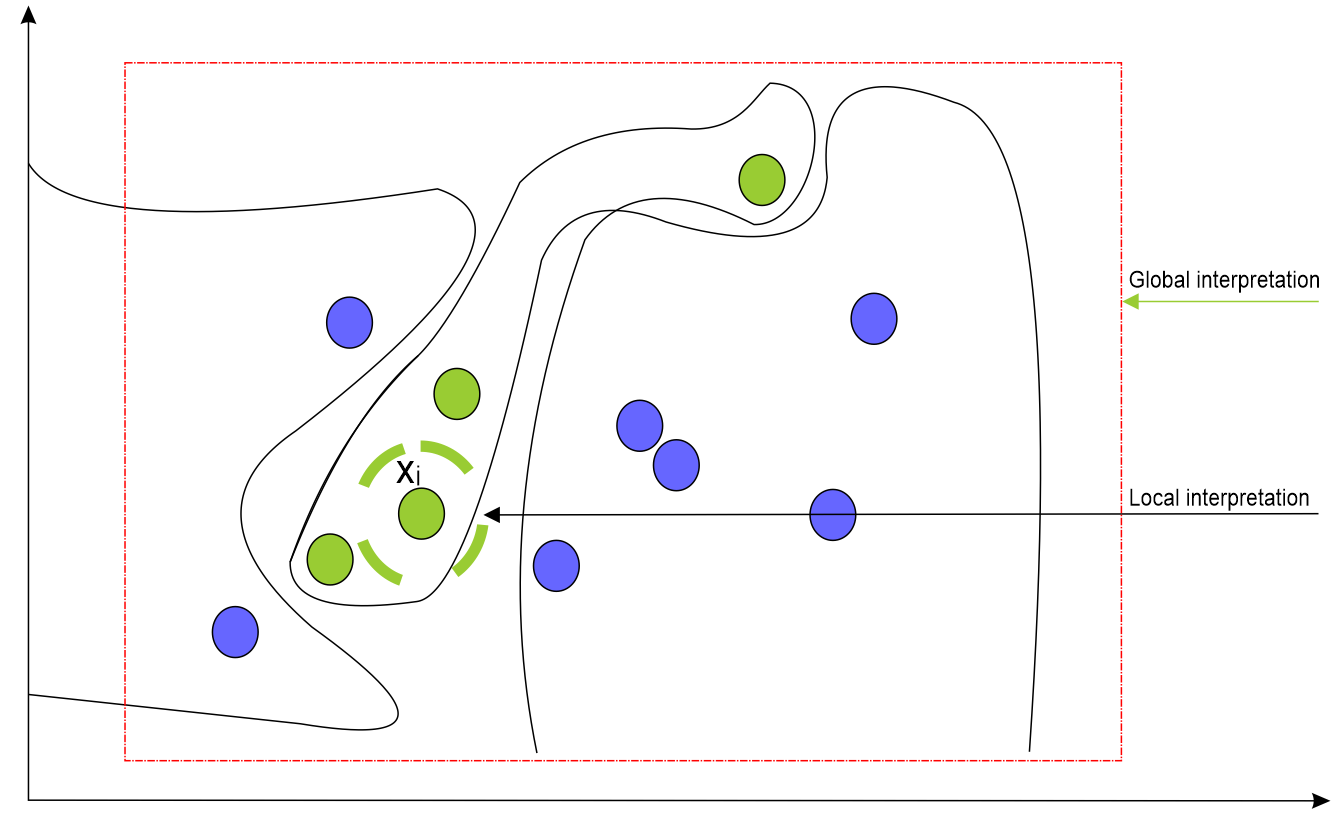
\includegraphics[width=0.6\textwidth,height=60mm]{images/lvg.png}\\ 
    \scriptsize{
        \textbf{Local interpretability:} why did the model make a certain prediction for an instance~\cite{molnar2019interpretable}? \\
         \textbf{Local interpretation:} being able to explain the conditional interaction between dependent and single prediction, i.e., focuses on explaining the prediction of an individual instance. 
        } 
\end{tcolorbox}
\fi 

%However, we can also classify such cases as either global if the subgroup is treated as the sub-population or as local if single prediction interpretations for the subgroup are grouped together~\cite{molnar2019interpretable}. 
\hspace*{3.5mm} A more concrete example related to the cancer diagnosis use case would be as follows: suppose, an ML model is trained to predict if a gene is up-regulated~(i.e., label) after some treatment based on the presence or absence of a set of regulatory sequences~(i.e., features). While a global interpretation strategy will tell you how important regulatory sequence $X_i$ is for predicting up-regulation across all genes in the dataset, a local interpretation strategy will tell you how important regulatory sequence $X_i$ is for predicting gene $y_i$ as up-regulated. As Azodi et al~\cite{azodi2020opening} suggest to emphasize on ML models identify association through correlation. This implicitly means that ML interpretation strategies do not necessarily meant to identify causal relationships between input features and labels. %\subsection{Model-specific vs. model-agnostic interpretability}

\begin{figure*}[h]
	\centering
	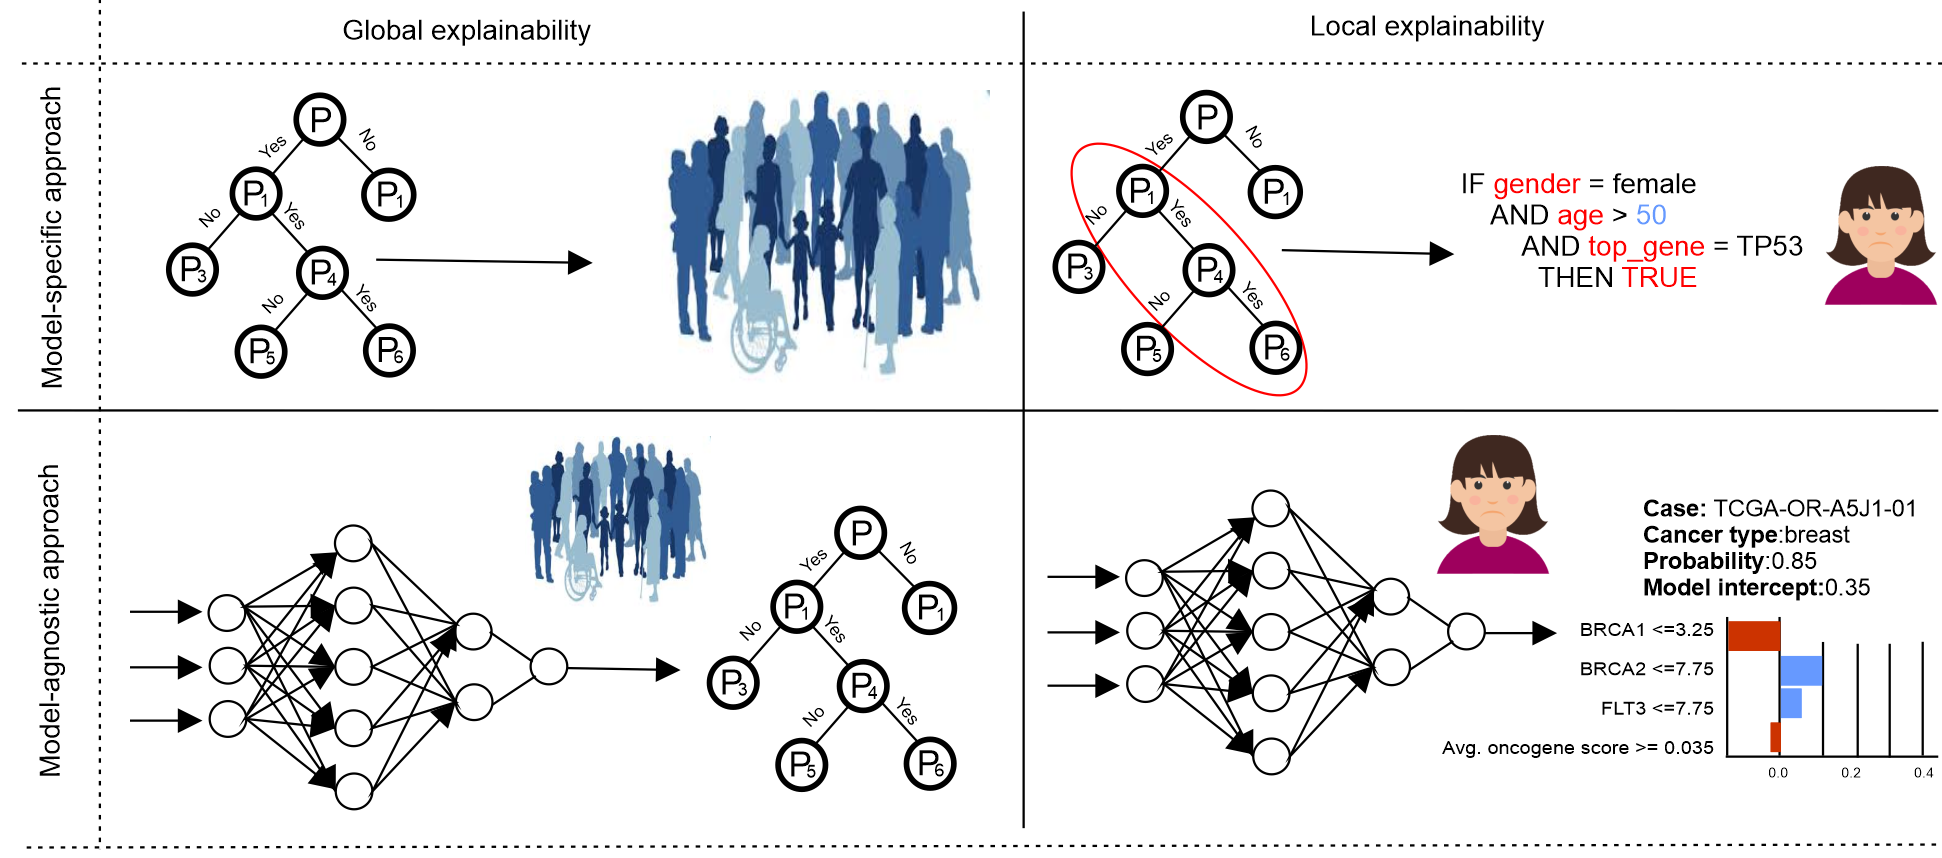
\includegraphics[width=0.9\textwidth,height=70mm]{images/lvg_cancer.png}	
    \caption{Scopes and types of ML models in healthcare based on their interpretability characteristics~(inspired by scopes and types by Stiglic et al.~\cite{stiglic2020interpretability}), showing an example of cancer types prediction}	
	\label{fig:local_vs_global_ex}
\end{figure*}

%\hspace*{3.5mm} Local interpretability of an ML model can be achieved by designing justified model architectures that explains why a specific decision was made or by providing similar examples of instances to the target instance~\cite{stiglic2020interpretability}. For example, for our cancer diagnosis use case, by emphasizing specific characteristics of a patient that represents the characteristics of a smaller group of cancer patients such as breast cancer, yet different in other patients~(rather than all the patients in a dataset).   In contrast, global interpretability signifies the overall transparency of the model inside a model on an abstract level. Nevertheless, an interpretable ML can be developed that can have cohort-specific interpretability, where they focus on population subgroups~\cite{stiglic2020interpretability}. 

%The former is limited to specific models by which the explanations can be derived by examining internal model parameters~\cite{stiglic2020interpretability}. The latter is, however, applicable on any ML model in a post-hoc manner~\cite{molnar2019interpretable}. 

\iffalse
\begin{figure*}[h]
	\centering
	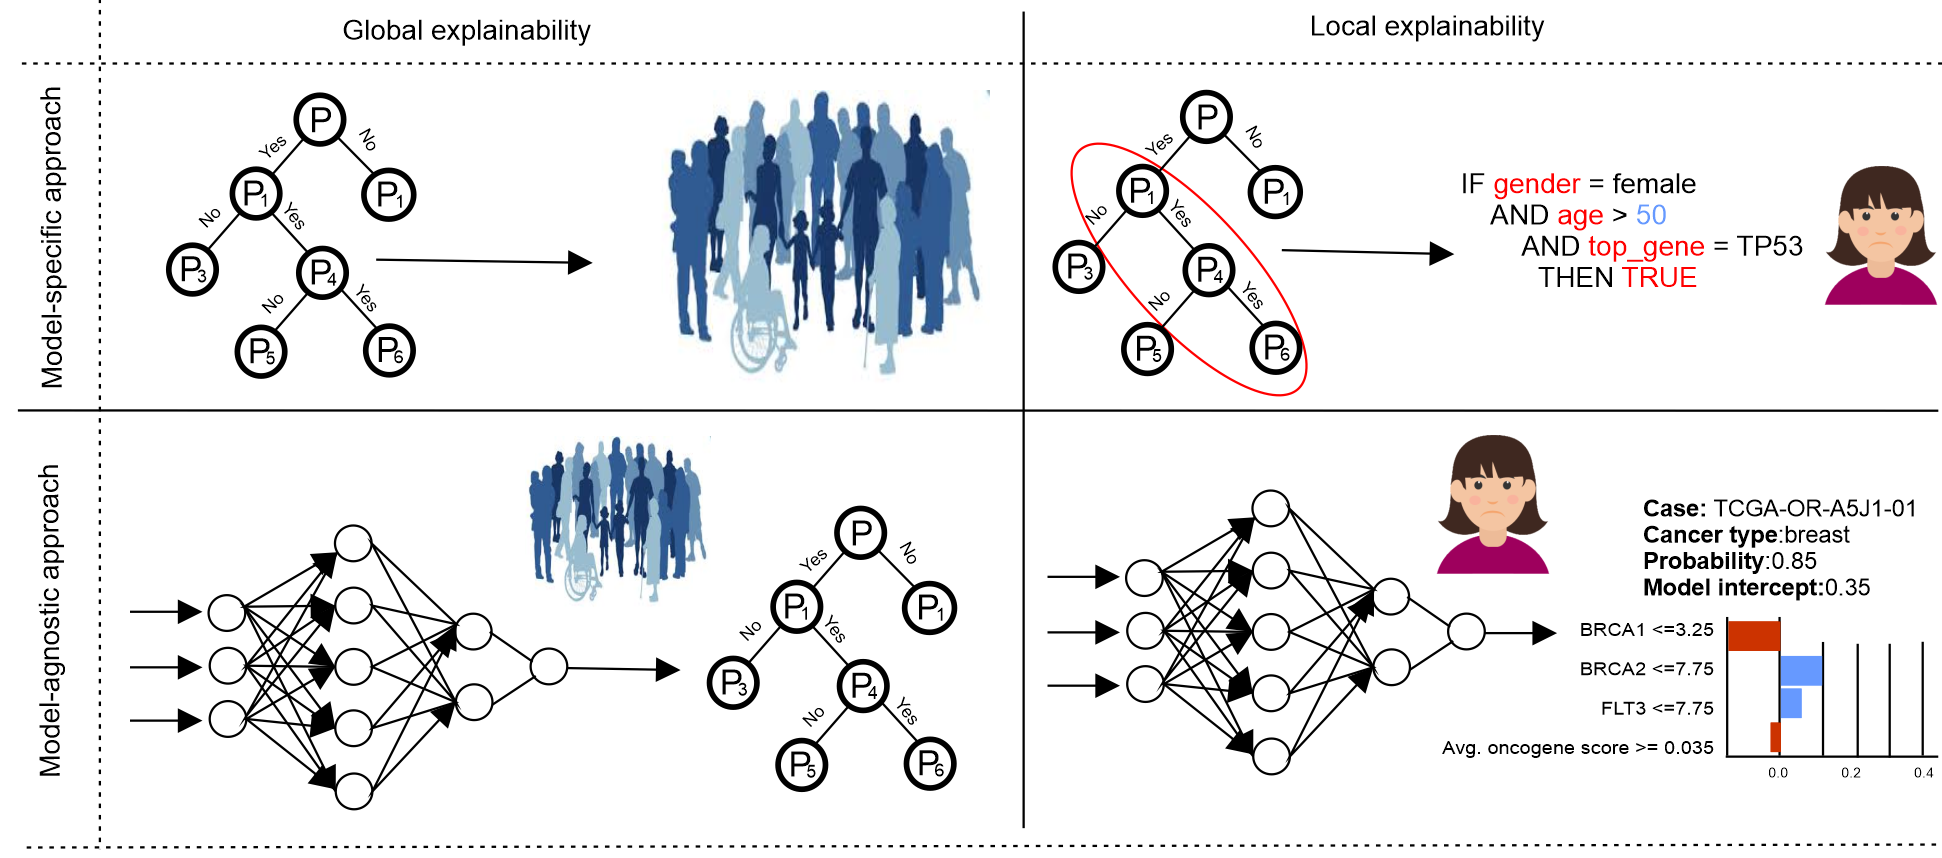
\includegraphics[width=\textwidth,height=70mm]{images/lvg_cancer.png}	
    \caption{Types of ML models in healthcare based on their interpretability characteristics (based on~\cite{stiglic2020interpretability}, showing an example of cancer types prediction}	
	\label{fig:local_vs_global_ex}
\end{figure*}
\vspace{2mm}
\begin{tcolorbox}[colback=white!3!white,colframe=gray!120!black,title=\faBook~Model surrogate]
    %INFO: \faBook \\
    \scriptsize{
        \textbf{Surrogate strategies:} model surrogation is a model interpretation strategies, which involve training an inherently interpretable model using the same data as a `black-box' model to approximate the predictions of the `black-box' model. }
\end{tcolorbox}
\fi 

\subsection{Techniques for interpretability}
Local interpretability of an ML model can be achieved by designing justified model architectures that explains why a specific decision was made or by providing similar examples of instances to the target instance~\cite{stiglic2020interpretability}. For example, for our cancer diagnosis use case, by emphasizing specific characteristics of a patient that represents the characteristics of a smaller group of cancer patients such as breast cancer, yet different in other patients~(rather than all the patients). In contrast, global interpretability signifies the overall transparency of the model inside a model on an abstract level. An interpretable ML can be developed that can have cohort-specific interpretability, where they focus on population subgroups~\cite{stiglic2020interpretability}. 

\hspace*{3.5mm} Based on outputs returned by the black-box model, \textit{surrogate} or a simple proxy model is often developed to learn a locally faithful approximation of a complex model~\cite{stiglic2020interpretability}. Model surrogation is a model interpretation strategy, which involve training an inherently interpretable model using the same data as a `black-box' model to approximate the predictions of the `black-box' model. Besides, probing and perturbing are also used as ML interpretation strategies, as shown in \cref{fig:pro_per_surroga}. Interpreting a model's outcome can be classified according to the results of the prediction model, as outlined by Molnar et al.~\cite{molnar2019interpretable}:

\vspace{-2mm}
\begin{itemize}[noitemsep]
    \item \textbf{Feature summary statistics} - summary of each feature and their impact on the model predictions. 
    \item \textbf{Feature summary visualization} - summary of the methods used to visualize and in order to make the visual communication easier, where outcomes are  presented with bars, plots, or table. 
    \item \textbf{Model internals approach} - the interpretation of intrinsically interpretable models, such as linear models in which model weights represent both internals parameters and summary statistics for the features. However, internal parameters of model-agnostic models are not typically inspected~\cite{molnar2019interpretable}. 
    \item \textbf{The data point interpretability} - methods that require data points themselves to allow interpretability to  return data points to make model interpretable. 
\end{itemize}

\hspace*{3.5mm} To explain and interpret the model predictions these ways, several approaches and methods have been proposed. 
\Cref{fig:xai_timeline} shows a timeline of XAI algorithms, covering scopes, methodology, and usage level~(based on~\cite{das2020opportunities}). In this subsection, we'll briefly cover most widely used ones. 
\subsubsection{Feature-based attribution methods}
\label{subsubsec:FI_shap}
For the human-level interpretability of a model, we need to know the inner insights, e.g., what features does a model think are most important and significant? Some of the features have higher impact than the others. This concept is called feature importance, which can be computed based on permutation importance~(PI). Intuitively, we can think of such importance both locally and globally, e.g., for a single prediction, we can compute the effect of each feature in the data, or, effect of each feature over a large number samples and overall the predictions.

\begin{figure}[h]
	\centering
	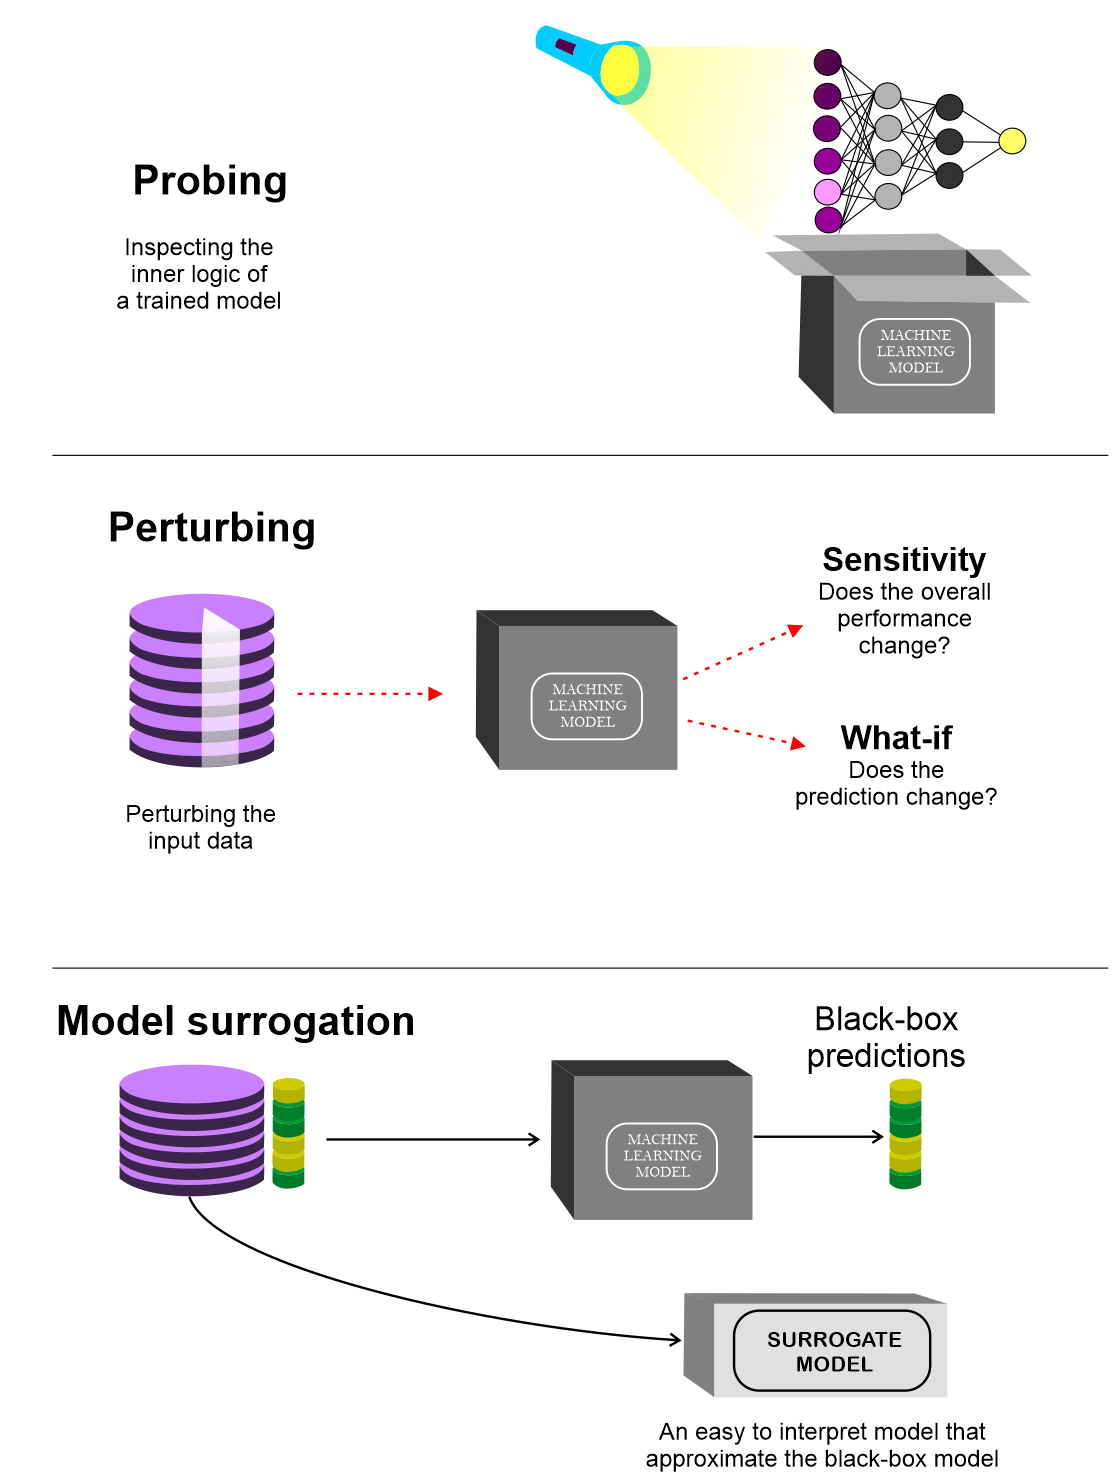
\includegraphics[width=0.8\textwidth,height=110mm]{images/pro_per_surrogation.png}	
    \caption{Different interpretability method for opening black-box ML model}	
	\label{fig:pro_per_surroga}
\end{figure}

\hspace*{3.5mm} Feature importance methods define an explanation function $g: F \times \mathbb{R}^{d} \mapsto \mathbb{R}^{d}$ that takes in a model $F$ and a point of interest $x$ and returns importance scores $g(F,x) \in \mathbb{R}^{d}$ for all features is the importance or attribution for feature $x_i$ of sample $x$. In other words, PI works by randomly permuting or shuffling a single column in the validation dataset leaving all the other columns intact, where a feature is considered ``important” if and only if the model's accuracy drops significantly and the error is increased. On the other hand, a feature is considered ``unimportant’ if shuffling its values does not affect the model's accuracy significantly. Explanation functions roughly fall into two categories: i) perturbation-based techniques, ii) saliency map and gradient-based techniques. 

\begin{sidewaysfigure*}
	\centering
	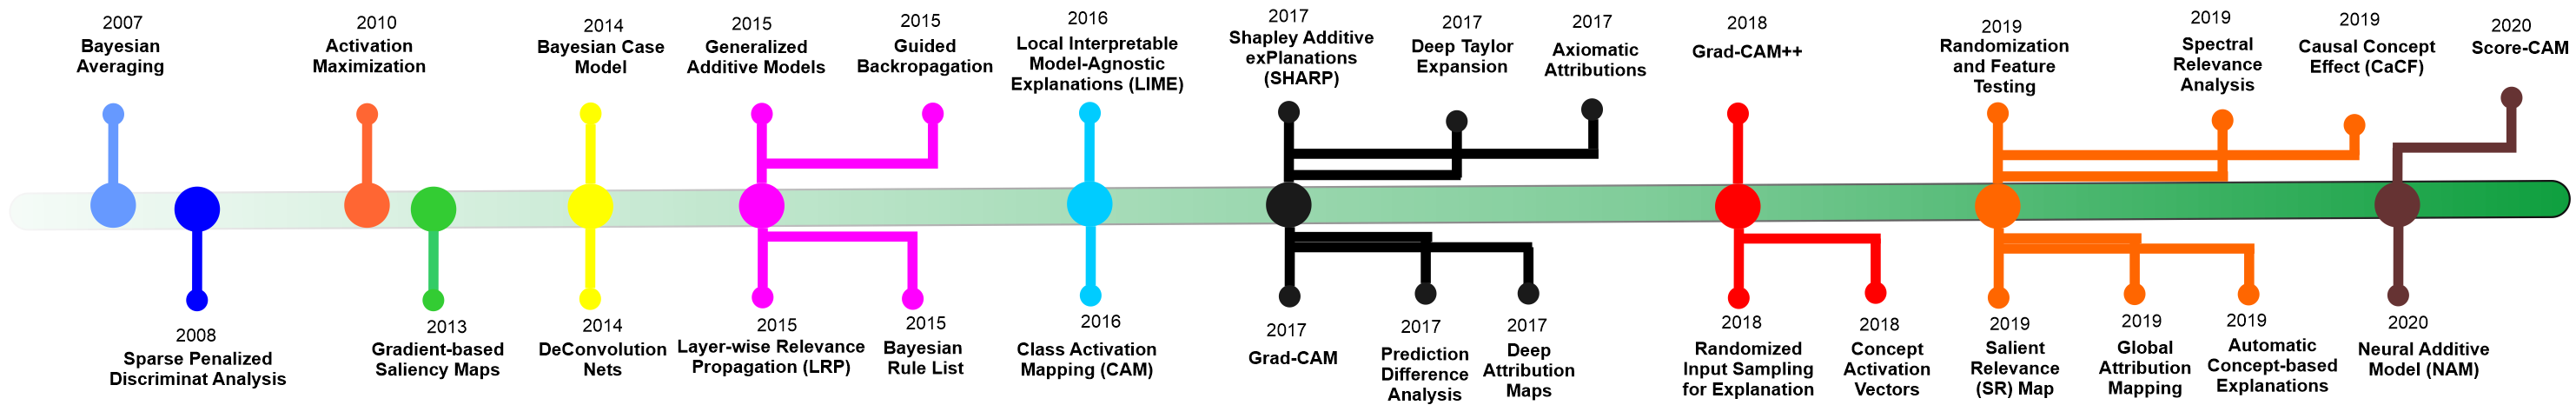
\includegraphics[width=0.8\textwidth,height=50mm]{images/xai_roadmap.png}	
    \caption{A timeline of XAI algorithms, covering scopes, methodology, and usage level~(based on~\cite{das2020opportunities})}	
	\label{fig:xai_timeline}
\end{sidewaysfigure*}

\hspace*{3.5mm} A widely used perturbation based methods is based on Shapley values inspired by cooperative game theory. A Shapley Value is the average marginal contribution of a feature value over all possible combinations of features which are used to estimate the Shapley value of a specific feature, whereas Shapley values are a way to distribute the gains to its players. SHapley Additive exPlanations~(SHAP) is a unified approach to explain the output of any ML model. SHAP connects game theory with local explanations, uniting several previous methods and representing the only possible consistent and locally accurate additive feature attribution method based on expectations~\cite{NIPS2017_7062}. 

\subsubsection{Saliency map and gradient-based attribution methods}
The saliency map and gradient-based attribution methods are used to identify relevant regions and assign importance to each input feature, e.g., pixel for image data. Typically first-order gradient information of a complex model w.r.t is used to produce maps that indicate the relative importance of the different input features for the classification. Gradient-weighted class activation mapping~(Grad-CAM)~\cite{selvaraju2017grad}, it's improved variant called Grad-CAM++~\cite{chattopadhay2018grad}, sensitivity analysis~(SA)~\cite{baehrens2010explain, simonyan2013deep}, and layer-wise relevance propagation~(LRP) are examples of this category. 

\subsubsection{Sensitivity analysis}
SA explains a prediction based on the model's locally evaluated gradient, aka. partial derivatives~(PD). Mathematically, SA quantifies the importance of each input variable $i$~(at low level, e.g., image pixel) $R_{i}=\left\|\frac{\partial}{\partial x_{i}} f(\mathbf{x})\right\|$. This measure assumes that most relevant input features are those for which the output is sensitive. Usually, a heatmap~(HM) is plotted to visualize and indicate which pixels need to be changed to make the image look similar to the predicted class. However, such HM does not indicate which pixels are actually pivotal for a specific prediction. Consequently, SA is not suitable for quantitative evaluation. 

\subsubsection{Grad-CAM, Grad-CAM++, and Score-CAM}
Guided backpropagation~(GB)~\cite{springenberg2014striving} is another method, where absolute values of the gradient of the output with respect to the input nodes are shown as heatmap, with the additional twist that negative gradients are set to zero at the rectification layers of the network is based on the fact is ``rectifying” the gradients in the backward pass leads to more focused heatmap~\cite{bohle2019layer}. While class-discriminating attention map visualization are appended to exhibit significant features for class assignment. To overcome the opaqueness of CNN, class activation maps (CAM)~\cite{zhou2016learning} is proposed. 

\hspace*{3.5mm} To explain where the model provides more attention, CAM computes the amount of weights of each feature map from the final conv layer. CAM calculates the contribution to prediction $y_c$ at location $(i,j)$, where the goal is to obtain $L_{ij}^{c}$ that satisfies $y^{c}=\sum_{i, j} L_{ij}^{c}$. The last feature map $A_{ijk}$ and prediction $y_c$ are represented in a linear relationship in which linear layers consist  of global average pooling (GAP) and FCL: i) GAP outputs $F_{k}=\sum_{i,j} A_{ijk}$, ii) FCL that holds weight $w_{k}^{c}$, generates the following output~\cite{kim2020extending}: 
 
 \vspace{-4mm}
 \begin{align}
     y^{c}=\sum_{k} w_{k}^{c} F_{k}=\sum_{k} w_{k}^{c} \sum_{i, j} A_{i j k}=\sum_{i, j} \sum_{k} w_{k}^{c} A_{i j k}.
 \end{align}
 \vspace{-4mm}
 
\hspace*{3.5mm} where $L_{i j}^{c}=\sum_{k} w_{k}^{c} A_{i j k}$~\cite{kim2020extending}. Subsequently, heat maps~(HM) are then plotted to visualize the weighted combination of the feature maps. However, if linear layers replace the classifier architecture, re-training of the network is required and non-linearity of classifier vanishes. Subsequently, literature~\cite{114} came up with an efficient generalization of CAM called Grad-CAM, where instead of pooling, globally averages gradients of feature maps as weights, w.r.t, aiming at class $c$. The guided backpropagation in Grad-CAM helps to generate more human-interpretable but fewer class-sensitive visualizations than the saliency maps~(SM)~\cite{nie2018theoretical}. Since SM use true gradients, trained weights are likely to impose a stronger bias towards specific subsets of the input pixels. Accordingly, class-relevant pixels are highlighted rather than producing random noise~\cite{nie2018theoretical}. Therefore, Grad-CAM is used to draw the HM to provide attention to discriminating regions, where the class-specific weights of each FM are collected from the final conv layer through globally averaged gradients~(GAG) of FMs instead of pooling~\cite{chattopadhay2018grad}: 

\vspace{-4mm}
\begin{equation}
    \alpha_k^c=\frac{1}{Z}\sum_{i}\sum_{j}\frac{\partial y^c}{\partial A_{ij}^k}.
    \label{eq:alpha}
\end{equation}
\vspace{-4mm}

\hspace*{3.5mm} where $Z$ is number of pixels in a FM, $c$ is gradient of the class, and $A_{ij}^k$ is the value of $k^{th}$ FM. Having gathered relative weights, the coarse SM, $L^c$ is computed as the weighted sum of $\alpha_k^c*A_{ij}^k$ of the ReLU activation and employ the linear combination to the FM, as features with only positive influence on the class are of interest~\cite{chattopadhay2018grad} and negative pixels that belong to other categories in the image are discarded~\cite{114}:

\vspace{-4mm}
\begin{equation}
    L^c=\operatorname{ReLU}(\sum_{i}\alpha_k^cA^k).
    \label{3.11}
\end{equation}
\vspace{-4mm}

\hspace*{3.5mm} However, if an image contains multiple occurrences with slightly different orientations or views of the same class, several objects would fade away in the saliency map created by Grad-CAM. Moreover, due to its overlooking at significance disparity among pixels, parts of objects are rarely focused by Grad-CAM. Grad-CAM++ is proposed~\cite{chattopadhay2018grad} to replace the GAG with a weighted average of the pixel-wise gradients since the weights of pixels contribute to the final prediction by applying the following iterators over the same activation map $A^k$, $(i,j)$ and $(a,b)$:

\vspace{-4mm}
\begin{align}
    \begin{aligned}
        w_{k}^{c}=\sum_{i} \sum_{j} \alpha_{i j}^{k c} \cdot \operatorname{ReLU}\left(\frac{\partial y^{c}}{\partial A_{i j}^{k}}\right) \\
        y^{c}=\sum_{k} w_{k}^{c} \cdot \sum_{i} \sum_{j} A_{i j}^{k} \\
        \alpha_{i j}^{k c}=\frac{\frac{\partial^{2} y^{\ell}}{\left(\partial A_{i j}^{k}\right)^{2}}}{2 \frac{\partial^{2} y^{c}}{\left(\partial A_{i j}^{k}\right)^{2}}+\sum_{a} \sum_{b} A_{a b}^{k} \frac{\partial^{3} y^{c}}{\left\{\left(\partial A_{i j}^{k}\right)^{3}\right\}}}.
    \end{aligned}
\end{align}

\hspace*{3.5mm} Although, CAM variants managed to steer clear of back-propagating gradients all the way up to inputs, gradients are essentially propagated only till the final conv layer. Besides, Grad-CAM and Grad-CAM++ are limited to specific architectures that uses average-pooling layer to connect conv layers to FCLs. 
Gradient for a DNN architecture can not only be noisy but also tends to vanish due to saturation in Sigmoid or the flat zero-gradient region in ReLU. One of the consequences is that gradient of the output w.r.t input or internal layer activation may be noisy visually which causes problems in the plain SM~\cite{wang2020score}. 
\hspace*{3.5mm} These apply to both Grad-CAM and Grad-CAM++. A recent approach called Score-CAM is proposed by Haofan Wang et al.~\cite{wang2020score}. While Grad-CAM and Grad-CAM++ use the gradient information flowing into the last convolutional layer to represent the importance of each activation map, Score-CAM utilizes the importance called Channel-wise Increase of Confidence~(CIC): Score-CAM considers a convolutional layer $l$ in a model $f$, given a class of interest $c$, \cref{3.11} can be rewritten $L_{\text {Score-CAM}}^{c}$ as follows: 

\vspace{-4mm}
\begin{align}
    L_{S c o r e-C A M}^{c}=\operatorname{ReLU}\left(\sum_{k} \alpha_{k}^{c} A_{l}^{k}\right).
\end{align}
\vspace{-4mm}

\hspace*{3.5mm} where $\alpha_{k}^{c}=C\left(A_{l}^{k}\right)$ and  $C(\cdot)$ denotes the CIC score for activation map $A_{l}^{k}$. Since the weights come from the CIC score corresponding to activation maps on target class, Score-CAM gets rid of the dependence on gradient. Score-CAM can localize both single and multi objects accurately. From application perspective, Grad-CAM tends to only capture one object in the image, Grad-CAM++ and Score-CAM can localize multiple objects, but SM of Score-CAM are more focused than Grad-CAM++~\cite{wang2020score}.

\subsubsection{Layer-wise relevance propagation}
LRP~\cite{LRP1} is based on an assumption that the likelihood of a class can be traced backwards through a network to the individual layer-wise nodes of the input~\cite{LRP2}. LRP identifies important pixels by running a backward pass in the neural network. The backward pass is a conservative relevance redistribution procedure, where nodes that contribute the most to the higher-layer receive most relevance from it. First, an image $x$ is classified in a forward pass. Relevance $R_{t}^{(L)}$ is then back-propagated using deep Taylor decomposition (DTD)~\cite{DTD} to generate a relevance map $R_{LRP}$. Assuming the network has $L$ layers and for layer $l$, $1,2,...,N$ are the nodes, $1,2,..,M$ are the nodes in layer $l+ 1$. The relevance $R_{n}^{(l)}$ at node $n$ in layer $l$ is recursively defined as follows~\cite{LRP2}.  

\vspace{-4mm}
\begin{align}
    R_{n}^{(l)}=\sum_{m} \frac{a_{n}^{(l)} w_{n, m}^{+(l)}}{\sum_{n^{\prime}} a_{n^{\prime}}^{(l)} w_{n^{\prime}, m}^{+(l)}} R_{m}^{(l+1)}.
    \label{eq:rn}
\end{align}

The node-level relevance in case of negative values is calculated using ReLU as follows~\cite{LRP2}:

\vspace{-4mm}
\begin{align}
    R_{n}^{(l)}=\sum_{m} \frac{x_{n}^{(l)} w_{n, m}^{(l)}-b_{n}^{(l)} w_{n, m}^{+(l)}-h_{n}^{(l)} w_{n, m}^{-(l)}}{\sum_{n^{\prime}} x_{n^{\prime}}^{(l)} w_{n^{\prime}, m}^{(l)}-b_{n^{\prime}}^{(l)} w_{n^{\prime}, m}^{+(l)}-h_{n^{\prime}}^{(l)} w_{n^{\prime}, m}^{-(l+1)}}.
    \label{eq:rn_neg}
\end{align}

The output layer relevance is calculated before the back-propagation as follows~\cite{LRP2}:

\vspace{-4mm}
\begin{align}
    R_{n}^{(L)}=\left\{\begin{array}{ll}
    {z_{t}^{(L)}} & {n=t}, \\
    {0} & {\text { otherwise.}}
    \end{array}\right.
    \label{eq:rn}
\end{align}

\hspace*{3.5mm} Shortcomings of LRP is that it only considers the target class for the calculation, which can lead to the miss-attribution of input regions to the relevance. To tackle the issue of discriminating the target object’s class with the non-target classes, a class contrastive improvement on LRP called contrastive LRP~(CLRP) is proposed~\cite{LRP3}. 

\begin{figure}[h]
	\centering
	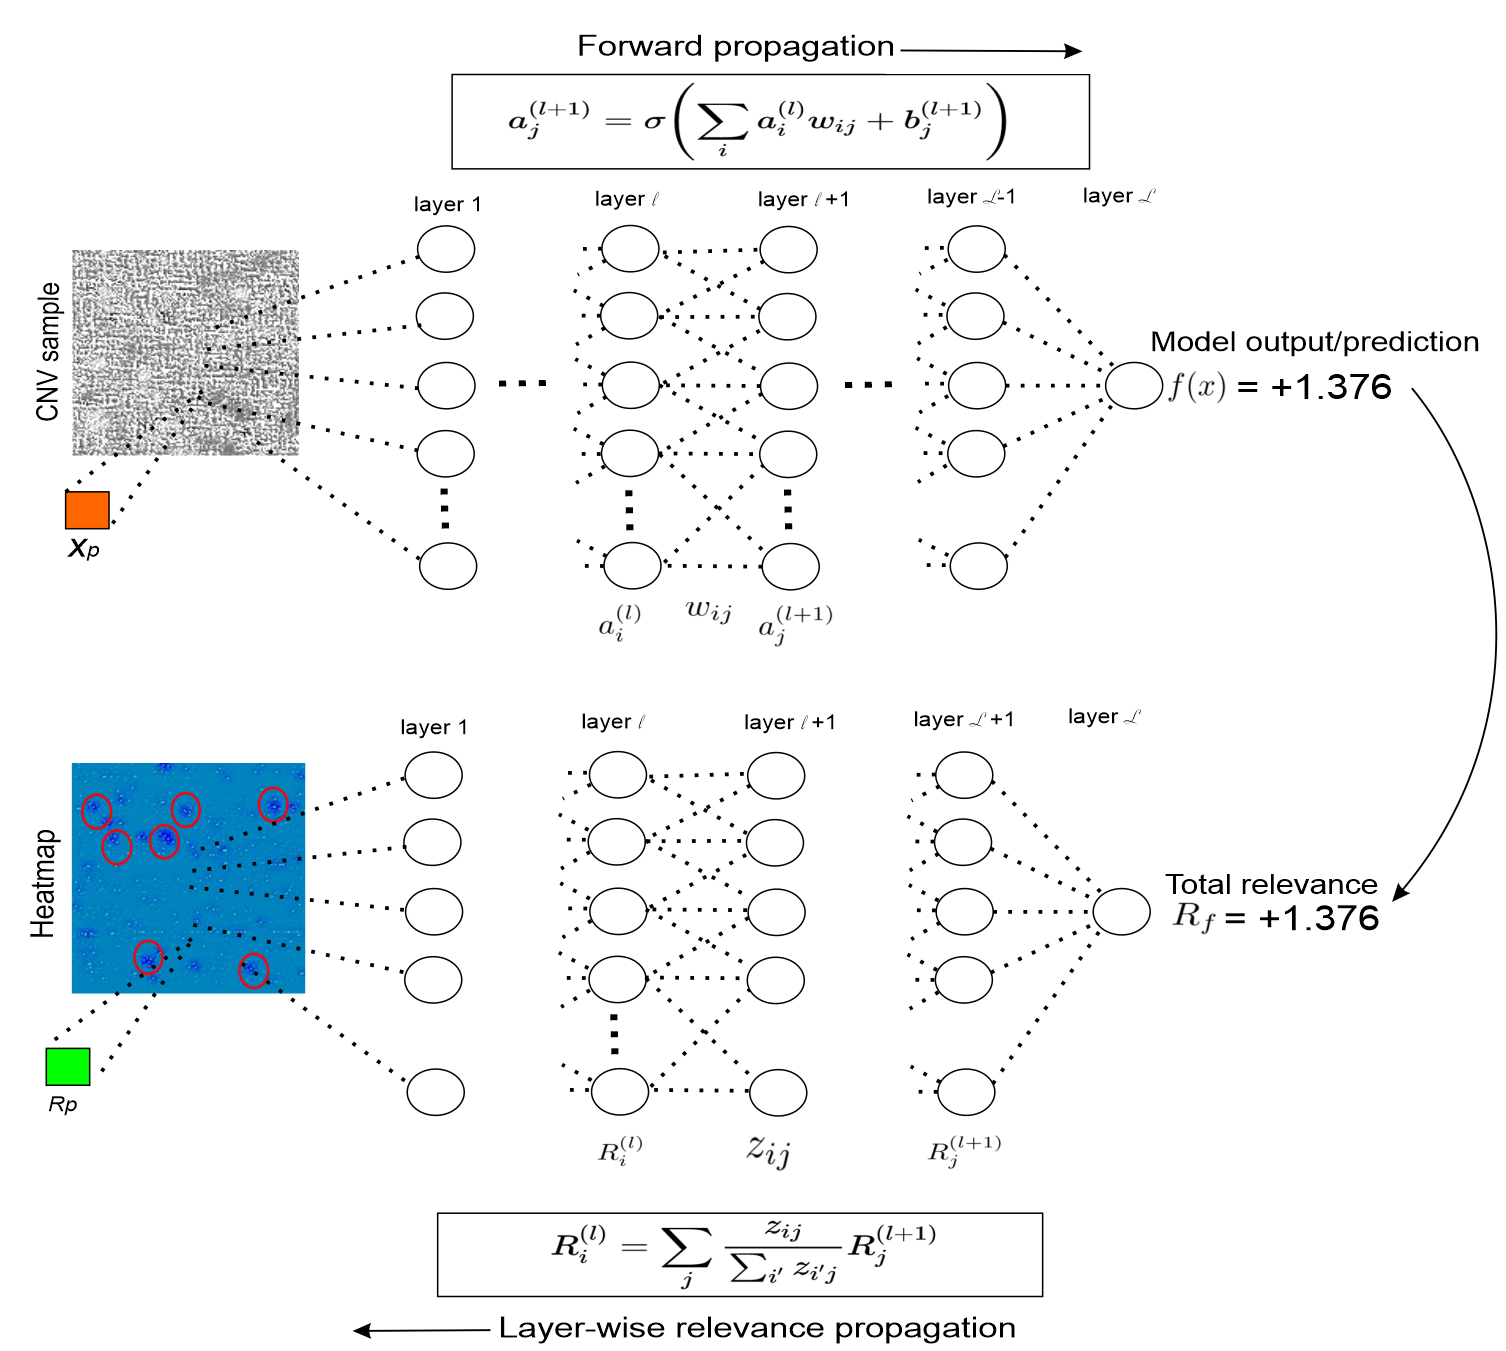
\includegraphics[width=0.8\textwidth,height=110mm]{images/lrp.png}	
    \caption{Overview of LRP for explaining model's decision, based on literature~\cite{binder2016layer}. First, the input image is processed , before the output/prediction is generated. Then, the output value is backpropagated layer-to-layer onto the pixel, where pixel relevances $R_p$ are visualized as heatmap.}	
	\label{fig:pro_per_surroga}
\end{figure}

\hspace*{3.5mm} By equally penalizing non-target classes, the relevance produced in CLRP is, however, reduced to zero, which is due to equal weighting of the non-target nodes~\cite{ LRP2}. Conversely, SGLRP is designed to take advantage of the post-softmax probabilities, where the gradient of the softmax output $\hat{y}_{t}$ is computed w.r.t, intermediate value of each output node $z_{n}$ as the relevance of the output layer $R_{n}^{(L)}$. The corresponding relevance map $R_{SGLRP}$ is then defined similar to \cref{eq:rn}, where $R_{1}^{(1)}, \ldots, R_{n}^{(1)}, \ldots, R_{N}^{(1)}$ are the relevance values at the input layer calculated by \cref{eq:rn} and \cref{eq:rn_neg}, except for the output layer relevance $R_{n}^{(L)}$, which is calculated as the gradient of softmax~\cite{LRP2}:

\vspace{-2mm}
\begin{align}
        R_{n}^{(L)}=\frac{\partial \hat{y}_{t}}{\partial z_{n}}=\left\{\begin{array}{ll}
        {\hat{y}_{t}\left(1-\hat{y}_{t}\right)} & {n=t}, \\
        {-\hat{y}_{t} \hat{y}_{n}} & {\text { otherwise.}}
    \end{array}\right.
\end{align}

\subsubsection{Decision rules-based explanations}
Due to the nested non-linear and complex structure, DNN architectures are mostly opaque and perceived as `black box' methods. They not only suffer from lack of transparency but also cannot reason about their underlying decisions. A DNN produces a prediction, which is an outcome of a bunch of mathematical expressions chained together that represent the way inner layers of an algorithm. However, using a set of rules, it possible to explain a decision intuitively to human with the ability to look up the reason for a decision. A \textit{decision rule} is a simple \textit{IF-THEN} statement consisting of a condition called antecedent and a conclusion~\cite{molnar2019interpretable}. The IF-THEN structure semantically resembles natural language and the way how human think~\cite{molnar2019interpretable}. Following are the characteristics of a decision rule: 

\begin{itemize}[noitemsep]
    \item \textbf{Structure} - follow a general structure: IF conditions are met THEN make a certain prediction. 
    \item \textbf{Number of condition} - a decision rule has at least one feature=value statement in the condition, with no upper limit and more statements can be added with an ‘AND’ operator. 
    \item \textbf{Single or multiple decision rules} - although a combination of several rules can be used to make predictions, sometimes a single decision rule is enough to explain the whole outcome.
\end{itemize}

\hspace*{3.5mm} If derived from intelligible features and the length of the condition is short, decision rules are probably the most interpretable prediction models. Suppose we have a simple model for predicting the body mass index~(BMI). Interpreting a predicted BMI with a decision rule is very easy and can be explained in layman term. For example, IF BMI $\geq$ 30~(condition), THEN you're obese~(prediction). Further explanations can be provided saying that ``an increased BMI is associated with risk for developing \textit{type-2 diabetes}, hypertension, and cardiovascular disease". 
On the contrary, even this simple concept may not be well understood by patients~\cite{post2015patient} themselves. Once we have a transparent and easily explainable AI model, decision rules can be generated using a series of IF-THEN statements. In this thesis, one of the goals is to generate human-interpretable decision rules automatically based on self-explanatory logic for all decisions. 

\subsubsection{Neuro-symbolic reasoning and challenges of current XAI methods}
Alejandro B. A, et al.~\cite{arrieta2020explainable} outline the trade-off between interpretability and accuracy, i.e., between the simplicity of the information given by the system on its internal functioning, and the exhaustiveness of this description
cognitive sciences to create objectively convincing explanations.
Explanations are better when constrictive, i.e., a good explanation is not only indicates why the model made a decision $\mathrm{X}$, but also why it made decision $\mathrm{X}$ rather than decision $\mathrm{Y}$. 

\hspace*{3.5mm}It is also explained that probabilities are not as important as causal links in order to provide a satisfying explanation. Considering that `black-box' models tend to process data in a quantitative manner, it would be necessary to translate the probabilistic results into qualitative notions containing causal links. Besides, counterfactual explanations can help the user to understand the decision of a model. In such a scenario, combining connectionist and symbolic paradigms is a promising way to address this challenge. On one hand, connectionist methods are more precise but opaque. On the other hand, symbolic methods are popularly considered less efficient, albeit they offer following features:

\begin{itemize}[noitemsep]
    \item It is possible to establish reasoning rules to allow symbolic methods to be constrictive.
    \item The use of a $\mathrm{KB}$ formalized by an ontology allows data processing in a qualitative way.
    \item Being selective is less straightforward for connectionist models than for symbolic ones.
\end{itemize}

\hspace*{3.5mm}The representation of the external reality using symbols, it seems obvious that the use of the symbolic learning paradigm is appropriate to produce an explanation. Therefore, neuro-symbolic interpretability could provide convincing explanations while keeping or improving generic performance. %An efficient explainable model enables users see the explanations that were already deduced based on the background knowledge. 
Having a semantic representation of the knowledge can help a model to have the ability to produce explanations. 

\iffalse
\subsection{Library and frameworks for interpretability}
\subsubsection{LIME}
Local Interpretable Model-agnostic Explanations~(aka. LIME) is an interpretable library to explain the predictions of any classifier or regressor. LIME explains the predictions by approximating it locally with an interpretable model. Additionally, LIME is is capable of explaining black-box classifiers, with two or more classes. 
\subsubsection{SHAP} 

\subsection{Measurements for explainability}
Unfortunately, there is little consensus on what interpretability in ML is and how to evaluate it for benchmarking. Current interpretability evaluation typically falls into two categories: 

\begin{itemize}[noitemsep]
    \item The first evaluates interpretability in the context of an application: if the system is useful in either a practical application or a simplified version of it, then it must be somehow interpretable~\cite{bhatt2020explainable}. 
    \item The second evaluates interpretability via a quantifiable proxy: a researcher might first claim that some model class—e.g. sparse linear models, rule lists, gradient boosted  trees—are interpretable and then present algorithms to optimize within that class~\cite{miller2018explanation}. 
\end{itemize}

\hspace*{3.5mm} To large extent, both evaluation approaches rely on some notion of ``you’ll know it when you see it'' or ``seeing is believing''. The notions of interpretability meet the first test of having face-validity on the correct test set of subjects: human beings. However, this is too naive that leaves many kinds of questions unanswerable, e.g., ``are all models in all defined-to-be-interpretable"? and ``are all model classes equally interpretable"? The simplistic answer to these questions would be defining some metrics for evaluating such an XAI model. Robert Hoffman et al.~\cite{hoffman2018metrics} proposed the following metrics/methods for evaluating such an XAI model, which we will try to answer in \cref{chapter:fairness}:

\begin{itemize}[noitemsep]
    \item The goodness of the explanations
    \item Whether users are satisfied by explanations
    \item How well users understand the AI systems
    \item How curiosity motivates the search for explanations
    \item Whether the user's trust on the AI is appropriate
    \item How the human-XAI work system performs.
\end{itemize}
\fi 

\section{Cancer Growth and Metastasis}
\label{cancer_growth}
Cancer is an umbrella term for a large group of lethal diseases. Till date, more than 200 types of cancer have been identified~\cite{82Tomczak}, making it the second leading cause of death worldwide~\cite{pancan}. According to a statistic from the National Cancer Institute\footnote{\url{https://www.cancer.gov/about-cancer/understanding/statistics}}, there were around 14.1 million cancer cases in 2012 in which as many as 8.8 million people died of five leading cancers of lung, liver, colorectal, stomach, and breast~\cite{stat}. In 2018, an estimated 17.35 million new cases of cancer have been diagnosed in the United States in which 609,640 people died. The number of new cancer cases per year is expected to rise to 23.6 million by 2030, which is anticipated to increase further by 70\% by 2035~\cite{71Torre}. 

\subsection{The growth of cancer}
In this section, we focus on the different types and subtypes of cancer and their growth and metastasis. The idea is to acquire some biological interpretations of the genomics data for our DSS. Cancer mainly caused when abnormal cells divide rapidly, and spread to other tissue and organs~\cite{pancan}. Cancer is often  driven by a series of genetic mutations of genes induced by selection pressures of carcinogenesis in the cells~\cite{ghazani2017assigning, baker2015cancer}. Those genes often called called marker genes ~(or biomarkers) include both onco- and tumor suppressor genes. When biomarkers over- or under-express in cancer cells as differentially expressed genes, they become uncontrollable proliferation or immorality of cancer cells~\cite{ghazani2017assigning, baker2015cancer}. 

\hspace*{3.5mm} Although the difference in the average of expression between two sample classes are often employed in many transcriptomics analyses, such difference is not the only way that a gene can be expressed differentially~\cite{xie2018adaptively}. In fact, there exist a number of regulators or mediators in cells such as transcriptional factors or miRNA, regulate a target gene in a collective way and accordingly shape a complex and heterogeneous expression pattern across inter- or intra-classes for the target gene~\cite{ghazani2017assigning, baker2015cancer}, albeit they work quite independently. Such regulatory mechanisms may account for the high biological variability where, for example, samples in one condition show a bi-modal pattern of expression versus the other condition which show a unimodal pattern of expression across samples~\cite{xie2018adaptively}. In a nutshell, following biological processes are mainly responsible for the growth of cancer: 

\begin{itemize}[noitemsep]
    \item \textbf{Minor mutations} - when a minor change happened to the DNA in the cells, our body cells correct these mistakes, by converting it into a healthy cell. However, when a mistake cannot be corrected, a cell can become cancerous. 
    \item \textbf{Major mutations} - when a minor change causes the cells to be replaced to survive instead of dying, and new cells to form when they're not needed. These extra cells can divide uncontrollably, causing growths called tumors~\cite{82Tomczak}. Besides, genetic mutations can be inherited. Cancer disrupts grow and divide process of healthy cells, which leads to abnormal growths~\cite{pancan}. 
    \item \textbf{Gene alterations} - changes in the structure of occurring genetic aberrations, such as somatic mutations, copy numbers~(CN), profiles, and different epigenetic alterations can form tumor or cancerous cells as they affect normal cell division and  growth~\cite{82Tomczak,13cancerdef,19Cruz}. 
%It’s caused by changes or mutations in DNA. DNA exists in the individual genes of every cell. It has instructions that tell the cell what functions to perform and how to grow and divide. 
\end{itemize}

\subsection{Cancer metastasis and subtypes}
When gene expression~(GE) is disrupted by cell division, environmental effects, or genetically inherited from parents, it also changes the production of different proteins, affecting normal cell behavior. Cancer cells that gone wrong no longer respond to many of the signals that control cellular growth and death. Subsequently, damaged cells start reproducing more rapidly than usual and gradually increase in the affected area by forming a tumor. Intermittently, such tumors turn into a type of cancer~\cite{zuo2019identification,24Podolsky}. Tumors can cause a variety of health problems, depending on where they grow in the body~\cite{zuo2019identification}. They can grow large and cause problems when they press against neighboring organs and tissue, although not all tumors are cancerous. During the early stages, tumors are typically benign\footnote{Benign tumors are noncancerous and do not spread to nearby tissues~\cite{o2010unit}} and remain confined within the normal boundaries of a tissue. When tumor grow and become malignant, they can break through these boundaries and invade adjoining tissues~\cite{o2010unit} and can invade other parts of the body~\cite{13cancerdef}. 

\hspace*{3.5mm} Cancers are named for the area in which they begin and the type of cell they are made of~\cite{19Cruz}, even if they spread to other parts of the body, e.g., a cancer that begins in the lungs and spreads to the liver is still called lung cancer. This process is called metastasis is how the cancer spreads to  different parts of the body from where it started growing~\cite{13cancerdef}. Some cancer cells can also migrate through the bloodstream or lymphatic system to distant areas of the body. When this spread over, an oncologist refers saying the cancer has ``metastasized"~\cite{22Ding}. Cancers that have metastasized are considered more fatal and advanced than those that have not, hence are harder to treat. On the other hand, cancer subtypes describes the smaller groups that a type of cancer can be divided into, based on certain characteristics of the cancer cells. Besides, there are several clinical terms used to describe certain types of cancer\footnote{\url{https://www.healthline.com/health/cancer\#types}}:

%\vspace{-4mm}
\begin{itemize}[noitemsep]
    \item \textbf{Carcinoma} is a cancer that starts in the skin or the tissues that line other organs.
    \item \textbf{Sarcoma} is a cancer of connective tissues, e.g., bones, muscles, and blood vessels.
    \item \textbf{Leukemia} is a cancer of bone marrow, which creates blood cells.
    \item \textbf{Lymphoma} and myeloma are cancers of the immune system.
\end{itemize} 
%\vspace{-4mm}

\hspace*{3.5mm} Although more than 200 types have been reported, cancer of bladder, breast, colon and rectal, endometrial, kidney, leukemia, liver, lung, melanoma, pancreatic, prostate, and thyroid are most common~\cite{71Torre}. 

\subsection{Genomics Data-based Diagnosis of Cancer}
Discovery of important biomarkers is a significant step towards understanding the molecular mechanisms of carcinogenesis and prognosis of certain cancer type. In cancer research, multimodal data and clinical outcomes need to be processed for understanding its genetic and epigenetic causes before diagnosis and recommending appropriate treatment. By acquiring insights from the omics data, treatment can be focused on preventive measures. Such multimodal data include omics, imaging~(e.g., histology and radiology), pathological reports, and clinical outcomes~\cite{22Ding, 23Zheng}. Genomics data such as somatic mutations, copy number variations~(CNVs), DNA methylation~(DM), gene expression~(GE), miRNA expression~(MR), and Isoform expression~(IEx) are more widely used~\cite{yates, ncbi1,ncbi2, kozomara1,kozomara2}.  
\hspace*{3.5mm} As the importance of genetic knowledge in cancer treatment is increasingly addressed~\cite{15Wu}, several projects have emerged. In particular, the next generation sequencing~(NGS) is playing a key role in therapeutic decision making for the cancer prognosis and treatment~\cite{jha2017towards}, leveraging a massive amount of sequencing omics. The cancer genome atlas~(TCGA)~\cite{tomczak2015cancer} is best known for omics data and is a collection of bio-molecules inside living things such as genomics, metabolomics, and proteomics. However, omics data are generated from multiplatform and heterogeneous sources, which needs to be analyzed to make clinical decisions, where both multimodality and heterogeneity impose great challenges to bioinformatics tools and computational algorithms~\cite{karimACCESS2019,karimBIB2019}. 
%Now that we already know about genomics data, up next we discuss each data types. 

\subsubsection{Gene and miRNA expression}
Due to  gene alterations and abnormal behaviors of genes, GE can be disrupted by cell division or environmental effects, or genetically inherited from parents. Changes in GE sometimes change the production of different proteins, affecting normal cell behavior. These damaged cells start reproducing more rapidly than usual and gradually increase in the affected area by forming a tumor. Intermittently, such tumors turn into a type of cancer~\cite{zuo2019identification,24Podolsky}. GE quantification data contains the amount of expression per gene for each patient based on ensembl gene identifiers, while miRNA expression quantification data contains the amount of miRNA expression for each patient based on miRNA identifiers. Following are different types of available data in TCGA, for each patient~\cite{ncbi1,ncbi2}: 

\begin{itemize}[noitemsep]
    \item  \textbf{Masked somatic mutations} - description of masked of SNV or SNP in which the data is categorized based on chromosome, gene, and position of SNP in base pair~(BP). 
    \item \textbf{Copy number segment} - amount of copy numbers based on on chromosome and position in BP. 
    %\item \textbf{Masked copy number segment} -amount of masked CNV. 
    \item \textbf{DNA methylation} - amount of methylated DNA per CpG probe identifiers. 
    \item \textbf{Gene expression} - amount of expression per gene based on ensemble gene identifiers. 
    \item \textbf{miRNA expression} - amount of miRNA expression based on miRNA identifiers. 
    \item \textbf{DNA methylation} -a amount of methylated DNA per CpG probe identifiers. 
    \item \textbf{Isoform expressions} - amount of isoform expression based on miRNA identifiers. 
    \item \textbf{Clinical} - clinical outcomes and records. 
\end{itemize}

\subsubsection{Copy number variations}
\label{sec:cnv_data}
Copy number variations~(CNVs) are gene or genomic regions that appear in different number of copies in different individuals or even in different cells of the same individual, where copy numbers can vary across individual by several thousand. About 5-12\% of the human genome, including thousands of genes, may be variable in copy number, and this variation can be de novo deletions or duplications of the genome or inherited from the parents by healthy individuals~\cite{ostrovnaya2010classification}, ranging in size from 100 bp to 3 Mb~\cite{zhang2006development}. Although the significance is not fully understood, it is likely that CNVs are responsible for a considerable proportion of phenotypic variation~\cite{ostrovnaya2010classification}. Such variations may lead to changes in gene dosage and expression~\cite{diskin2009copy}. Approximately 179,450 human CNVs have been reported in the Database of Genomic Variants~\cite{iafrate2004detection,zhang2006development}. Although these reported CNVs are substantially fewer reported than SNPs, it is estimated that more than 30\% of the human genome is covered by at least one CNV~(compared to the $<1$\% covered by SNPs). Due to the CN changes in DNA segments, gene expression is changed by disrupting coding sequences, perturbing long-range gene regulations or altering gene dosages~\cite{37Yang}. CNVs result in variations in gene expressions and abnormalities in the human phenotypes~\cite{18Chen}. 
%Thus, CNVs are hypothesized to be of functional significance. These changes in gene expressions are responsible for different phenotypic variations or disease such as disabilities, diabetes, cancer, obesity, and autism spectrum disorder~\cite{38Buckland, 39Nguyen, 40McCarroll}. 
%CNVs are also associated with other complex disease susceptibility. For example, changes in gene 3p25 and 2p24.3 found to be responsible for prostate cancer aggressiveness~\cite{43Liu, 44Thean}; changes in gene expression of the BRCA group are considered to be responsible for breast and ovarian cancer~\cite{45Petrij, 46Montagna}; deletions of GSTM1 and GSTT1 are proven to be responsible for decreasing the five-year cancer survival rate in Dutch people who have prostate cancer and bladder cancer~\cite{48Diskin, 31Park}.

\iffalse
\begin{table*}[h]
	\begin{center}
		\caption{different types of publicly available genomics data in TCGA}
		\label{tab:tcga_data_all_des}
		%\resizebox{\textwidth}{!}{
		\vspace{-2mm} 
			\begin{tabular}{| l | l |} 
				\hline
				\multicolumn{1}{|c|}{\textbf{Data type}} & \multicolumn{1}{c|}{\textbf{Description}} \\ 
				\hline
				Masked somatic mutations & \multicolumn{1}{p{10cm}|}{Description of masked (without germline mutation) of single nucleotide variation~(SNV) or Single nucleotide polymorphism~(SNP) for each patient in which the data is categorized based on chromosome, gene, position of SNP in base pair.} \\
				\hline
				Copy number segment & \multicolumn{1}{p{10cm}|}{Amount of copy numbers for each patient based on chromosome, and position of CNV in base pair.} \\
				\hline
				Masked copy number segment & \multicolumn{1}{p{10cm}|}{Amount of masked (without germline mutation) CNV for the patients.} \\
				\hline
				DNA Methylation & \multicolumn{1}{p{10cm}|}{Amount of methylated DNA for each patient per CpG probe identifiers~\cite{ncbi1,ncbi2}.} \\
				\hline
				Gene expressions & \multicolumn{1}{p{10cm}|}{Amount of expression per gene for each patient based on ensembl gene identifiers~\cite{yates}.} \\
				\hline
				miRNA expressions & \multicolumn{1}{p{10cm}|}{Amount of miRNA expression for each patient based on miRNA identifiers~\cite{kozomara1,kozomara2,griffiths-jones1,griffiths-jones2,griffiths-jones3}.} \\
				\hline
				Isoform expressions & \multicolumn{1}{p{8cm}|}{Amount of isoform expression for each patient based on miRNA identifiers.} \\
				\hline
				Clinical & \multicolumn{1}{p{8cm}|}{Clinical outcomes and records of the patients.} \\
				\hline
		\end{tabular}%}
	\end{center}
\end{table*}
\fi 

\hspace*{3.5mm} These became more obvious because CNVs are associated with the risk of individual cancer~\cite{cnv11,cnv12,cnv13}. For example, CNVs that play a role in genetic predisposition to pancreatic adenocarcinoma~\cite{cnv13} are associated with breast cancer risk and prognosis~\cite{cnv12} and are responsible for the spatial pattern change in colorectal cancer~\cite{cnv11}. This is because the presence of CNVs in cancer patients’ cells is abundantly high, which is very different than healthy cells. Consequently, many clinically important CNVs are outcomes of duplication or deletion of a genomic region with at least 1Kb~(or shorter) in length. The CNVs related data used in this thesis include copy number segment~(CNS), which is the amount of CNVs for each patient based on chromosome, and position of CNV in base pair. On the other hand, the masked CNS contains the amount of masked, i.e., without germline mutation CNV for each patient.

\subsubsection{DNA methylation}
An altered DNA methylation pattern can have a severe impact on the behaviour of a cell by changing the binding affinity of transcription factors~(TF) and thereby intervene in GE. By silencing genes which code information for proteins involved in DNA repair, cell cycle regulation or suppression of metastasis, DNA methylation can also support oncogenesis. The changes in the DNA methylation pattern resulting in this can either occur prior to cell mutation or following it. Subsequently, either they initiate cancer development or they support it. Since the influence of DNA methylation is generally limited to only decrease the rate at which the respective protein is created, its role in the expression of genes relevant for cancer development is known to be more of quantitative character. The DNA methylation data used in this thesis contains the amount of methylated DNA for each patient per CpG probe identifiers. 

%\subsubsection{Other genomics data}
%Other types of genomics data that are used in cancer research includes masked somatic mutation data. These data provides the description of masked, i.e., without germline mutation of Simple SNV or SNP for each patient. Data is categorized based on chromosome, gene, position of SNP in base pair. The isoform expression quantification contains the amount of isoform expression for each patient based on miRNA identifiers. %\subsubsection{Characteristics of genomics data}

\section{Characteristics of genomics data}
In order to develop a DSS for clinical setting, we need to know the data as well as the mechanism for which the diagnosis decision will be based on. First of all, some types of cancer run in certain families. However, majority cancer types are not clearly linked to the genes, but we inherit from our parents. Therefore, this thesis will not consider family history records. Instead, we will mostly use the omics data and clinical information from one of the well-known project called PanCancerAtlas~(PCAt). PCAt covers multi-platform genomic measurements from 33 different cancer types~\cite{pancan}. 
%Therefore, we will use the PCAt data, due to availability and quality. 
The expression datasets in PCAt have unique characteristics that are different from text, images, or relational datasets. In particular, genomics data from PCAt show the following characteristics~\cite{lu2003cancer}:

\vspace{-2mm}
\begin{itemize}[noitemsep]
    \item \textbf{High dimensionality} - up to tens of thousands of genes.
    \item \textbf{Very small sample size} - less than $100$.
    \item \textbf{Very sparse feature space} as majority of genes are not responsible for cancer, i.e., not related to cancer types classification.
\end{itemize}
\vspace{-2mm}

\hspace*{3.5mm} With such a huge feature space, even a robust classifiers built upon, would prone to overfitting, due to small sample size~\cite{lu2003cancer}. Since most genes are known to be irrelevant for class distinction, their inclusion would not only introduce noise and confuse the classifiers, but also increase the computation time~\cite{lu2003cancer}. Therefore, feature selection and ranking of biologically meaningful biomarkers prior to classification would help in alleviating these problems. Nevertheless, with the `noise' from the irrelevant genes removed, the biological information hidden within will be less  obstructed~\cite{lu2003cancer}. 
%With high-throughput technologies such as next-generation sequencing~(NGS), cancer-specific genetic profiling is now possible. The entire genome sequencing data using NGS can be used to identify similar genetic mutations and genetic variations associated with different tumors. %\subsection{Data availability}
%As mentioned, different types of genomics data are used in cancer research, including somatic mutations, CNV, DNA methylation~(DM), gene expression~(GE), miRNA expression~(MR), and Isoform expression~(IEx), along with clinical outcomes. 
The largest uniformly processed cancer genomic data provided is TCGA, giving over 20,000 tumor and normal samples, where each step in the genome characterization pipeline generate following data points\footnote{\url{https://www.cancer.gov/about-nci/organization/ccg/research/structural-genomics/tcga/using-tcga/types}}:

\begin{itemize}[noitemsep]
    \item Clinical information, such as treatment information, survival data, etc. 
    %Besides, pathology reports were collected for selected sampels. 
    \item Molecular analyte metadata,e.g., sample portion weight.
    \item Molecular characterization data, e.g., gene expression values.
    %\item Patient phenotype and demographic information~(e.g., age, height, race, etc.). 
    \item Demographic information for the characterization of the patient by means of segementing the population, e.g., characterization by age, sex, or race\footnote{\url{https://docs.gdc.cancer.gov/Data_Dictionary/viewer/\#?view=table-entity-list&anchor=clinical}}.
    \item Diagnosis data from the investigation, analysis and recognition of the presence and nature of disease, condition, or injury from expressed signs and symptoms. 
    \item Family history - record of a patient's background regarding cancer events of blood relatives.
\end{itemize}

\section{Chapter Summary}
In this chapter, we provide preliminaries and several aspects required for the foundation of an AI DSS. We covered basics of decision support systems, machine learning, deep learning and neural networks, hyperparameter tuning, representation learning, neural ensemble methods, explainability and interpretability, different interpretable methods, and the mechanism of cancer growth and metastasis. 
It is now understandable that cancer is not only a lethal disease, but also tremendously complex to diagnose and treat. Therefore, not only recommending accurate diagnosis, but also knowing the biological mechanisms is important, e.g., oncogenes in order to provide subsequent treatments. 

\hspace*{3.5mm} Nevertheless, as research suggested~\cite{alirezaie2019semantic} that introducing semantics into deep learning model through ontological-reasoning will likely start a new era towards XAI, where the ML model reads input data, generates the predictions, observe the results, use the existing knowledge from the KB as a semantic reasoner, and produces new knowledge to provide more human-interpretable answers and explanations. The benefit is that the model learns not only from the data but also from explicit and encoded prior knowledge, which not only helps avoiding making similar mistakes in successive iterations, but also helps reducing the biases. 
Eventually, if an explainable DSS system can explain its reasoning, we can verify whether that reasoning is sound with respect to these auxiliary criteria for real clinical setting. 

\hspace*{3.5mm}In the next chapter, we start our explainable journey towards developing a DSS to leverage the cancer diagnosis and making the decision explainable and trustworthy.~We will use CNV data~(i.e., single modality) and investigate whether it effectively helps to predict cancer types. We will employ neural ensemble method to make the prediction pipeline robust. 
%\chapter{Related Work}\label{chapter:rw} 
\textit{``Knowing what you don’t know is more useful than being brilliant''}-Charlie Munger \\

\section{Overview}
In this chapter, we provide the summary of related works on interpretable machine learning approaches with a focus of cancer genomics and bioimaging. 

\section{Related Work}
\label{rw}
\subsection{Cancer typing methods}
Numerous approaches using mixed data types such as genomic data, bioimaging data, and clinical outcomes are used for analyzing genomics data and decision making for the cancer treatment~\cite{min}. For example, RNA-Seq data is used widely to identify rare and common transcripts, isoforms, and non-coding RNAs in cancer. Whereas, single-nucleotide polymorphism~(SNP) indicates small genomic variations in cancer patients and array-based DNA methylation data is used to provide epigenetic changes in the genome that are useful for early genetic changes of cancer e.g. early-stage detection of ovarian cancer is now possible~\cite{82Tomczak,95Gaul}. 

\hspace*{3.5mm}
Since DL algorithms can work better with such high dimensional data, recent studies focused on using deep neural networks~(DNN) architectures such as autoencoder, Restricted Boltzmann Machine~(RBM), Deep Belief Networks~(DBN), Multilayer Perceptron~(MLP), CNN, and Recurrent Neural Networks~(RNN) in cancer genomics. For example, literature~\cite{17Danaee} used Stacked Denoising Autoencoder to extract features from the RNA-seq data, which are then fed into SVM and shallow ANN to classify malignant or benign tumor of breasts~\cite{18Chen}. DeepCNA is another CNN-based approach proposed for cancer type prediction based on CNVs and chromatin 3D structure with CNN~\cite{yuan2018cancer}. Albeit, it is very efficient in the case where both CNA and 3D chromatin structures supplied, availability of such resources, however, not always possible as genomics-based cancer detection. 

\hspace*{3.5mm}
Besides, histology and radiological images are used for understanding the genetic and epigenetic cause in cancer analysis~\cite{yuan2018cancer,20Rajanna,23Zheng}. In particular, GISTIC, MutSig, and clustering algorithms are used to visualize genomic and transcription alterations in various cancers at advanced level~\cite{wb}. Besides, X-ray and CRT images~\cite{25Cruz} along with proteomic and genomic assays are also used, which shows great success in cancer prediction and prognosis~\cite{28Zhou}. Often these images are used to generate noninvasive, functional, and molecular imaging modality data called multispectral photoacoustic imaging~\cite{20Rajanna} to detect prostate cancer using K-means and SVM~\cite{23Zheng}. Besides, histopathology images are used~\cite{19Cruz, xu} to identify the existence of cancer using CNN. Literature~\cite{17Danaee} used stacked denoising autoencoder to extract features from RNA-seq data and then fed into SVM and shallow ANN to classify malignant or benign tumor of breasts~\cite{18Chen}. DeepCNA is another CNN-based approach for cancer type prediction based on CNVs and chromatin 3D structure~\cite{yuan2018cancer}. 

\hspace*{3.5mm}
Apart from these works, restricted methods have been proposed based on CNVs for cancer risk and type predictions~\cite{ding2014application, zhang2016classification, elsadek2018supervised}. Xiaofan D. et al~\cite{ding2014application} used recurrent CNVs from non-tumor blood cell DNAs of non-cancer subjects about hepatocellular carcinoma, gastric cancer, and colorectal cancer patients. They found to reveal the differences between cancer patients and controls concerning CN losses and CN gains. Although their study can make predictions on the cancer predisposition of an unseen test group of mixed DNAs with high confidence, it is limited to only Caucasian cohort and Korean cohorts. 

\begin{table*}[!ht]
    \caption{different cancer detection methods, data types, and performance }
    \label{table:stateofart}
    \begin{center}
    \scriptsize
    \vspace{-6mm}
    \begin{tabular}{l|l|l|l|l|l}
        \hline
        \textbf{Reference} & \textbf{Approach} & \textbf{Cancer types} & \textbf{\#Sample} & \textbf{Data type} & \textbf{Accuracy} \\\hline
            Karim et al.~\cite{karim2018a2ic} & DBN/LSTM & 14 primary types & 15,699 & TCGA CNVs & 73\% \\\hline % 2018
            Yuan et al.~\cite{yuan2018cancer} & CNN & 25 primary types & 14,703 & CNA \& 3D cromatin & 90\% \\\hline % 2018
            Sanaa et al.~\cite{elsadek2018supervised} & LR & 6 primary types & 3,480  & CNVs & 85\% \\\hline % 2018
        	Cruz et al.~\cite{19Cruz} & CNN & Breast cancer  & 605 & Slide images & 96\%  \\\hline  % 2017
            Danee et al.~\cite{17Danaee} & MLP & Breast cancer & 1210 & RNA-seq & 94\% \\\hline % 2016
            Ning et al.~\cite{zhang2016classification} & Dagging & 6 primary types & 3,480  & CNVs & 75\% \\\hline % 2016
        	Rajana et al.~\cite{20Rajanna} & Deep NN & Prostate cancer & 807 & Histology & 95\%\\\hline
            Chen et al.~\cite{18Chen} & Shallow NN & Colon cancer  & 590 & Gene expression & 84\% \\ \hline % 2015
            Ahmed et al.~\cite{abdel2016breast} & DBN & Breast cancer  & 569 & Wisconsin BRCA & 99\% \\ \hline % 2015
            Zheng et al.~\cite{23Zheng} & K-means/SVMst cancer & Phenotype & 569 & Wisconsin BRCA & 97.38\% \\ \hline % 2014
            Xiaofan et al.~\cite{ding2014application} & Naïve Bayes & Cancer risk & 640 & Human SNP & 93\% \\ \hline % 2014
        \end{tabular}
    \end{center}
\end{table*}

\hspace*{3.5mm}
Ning Z. et al.~\cite{zhang2016classification} used CNVs level of 23,082 genes for 2,916 instances from cBioPortal for Cancer Genomics to classify six different types of cancers, i.e., breasts, bladder urothelial, colon, glioblastoma, kidney, and head and neck squamous cell. They construct a dagging-based classifier in which the feature space was reduced into CNVs of 19 genes using minimum redundancy maximum relevance feature selection~(mRMR) and incremental feature selection~(IFS) methods~\cite{zhang2016classification}. Their approach managed to achieve an accuracy of 75\%, which indicates that only a few genes may play essential roles in differentiating cancer types. Sanaa et al.~\cite{elsadek2018supervised} extended their work in which 7 ML classifiers were trained giving random forest algorithm accuracy of 86\%. Other works used omics data to identify various cancer types e.g. literature~\cite{fakoor} used principal component analysis~(PCA) to extract features from high dimensional GE data, which are then fed into sparse and stacked autoencoders to classify acute myeloid leukemia, breast, and ovarian cancer patients. Whereas, literature~\cite{ibrahim} proposed a multilevel feature selection technique based on DBN and unsupervised active learning from miRNA expression data, which outperforms PCA-based methods for hepatocellular and breast carcinoma identification.

\hspace*{3.5mm}
For analyzing genomics data and decision making for cancer treatment, different ML and DL algorithms were trained using mixed data types, such as genomic data, bioimaging data, and clinical outcomes, as shown in \cref{table:stateofart}. These approaches are not only proven to be useful at improving cancer prognosis, diagnosis, and treatments, but also revealed the subtypes information of several cancer types~\cite{66Huang}. For example, RNA-seq data are used more widely to identify rare and common transcripts, isoforms, and non-coding RNAs in cancer. Single nucleotide polymorphism~(SNP) data are used to identify segmental variations across multiple cancer genomes, and array-based DNA methylation sequencing is used to provide epigenetic changes in the genome that are useful for early genetic changes of cancer (e.g., early-stage and metabolomic detection of ovarian cancer is now possible~\cite{82Tomczak,95Gaul}). 

\hspace*{3.5mm}
Unlike conventional cancer typing methods that work on analyzing morphological appearances, gene expression levels of the tumor are used to differentiate tumors that have similar histopathological appearances giving more accurate tumor typing results for the colorectal cancer diagnosis~\cite{paroder2006na+}. Different types of somatic mutations data such as point mutation, single nucleotide variation~(SNV), small insertion and deletion~(INDEL), copy number aberration~(CNA), translocation, and CNVs are also used. Literature~\cite{yuan2018cancer} has observed that these types of genomics data are not only associated with complex diseases but also with contribute to the growth of different types of cancers. In particular, literature~\cite{67Calcagno} studied CN changes by comparing healthy and cancer-affected patients, which showed that amplification and deletion of certain genes are more common in certain cancer patients than healthy people. It has been identified that CNVs are associated with the risk of pancreatic cancer~\cite{66Huang}. Imaging data such as histology and radiological images are used for understanding genetic and epigenetic causes in cancer analyses~\cite{yuan2018cancer,20Rajanna,23Zheng}. In particular, GISTIC, MutSig, and clustering algorithms are used to visualize genomic and transcription alterations in various cancers at an advanced level~\cite{wb}. X-ray and CRT images~\cite{25Cruz}, along with proteomic and genomic assays, are also used, which show great success in cancer prediction and prognosis~\cite{28Zhou}. These types of images are used to generate noninvasive, functional, and molecular imaging modality data called multispectral photoacoustic imaging~\cite{20Rajanna} in order to detect prostate cancer using K-means and SVM~\cite{23Zheng}. 

CNVs analysis based on different statistical methods are also used to identify significant CN associated with different types of cancers. For example, Fisher's exact~(FE) test is applied on patient and control groups to identify copy numbers for hereditary breast and ovarian cancer~\cite{58Kuusisto}. Although FE is mainly used for CNV analysis~\cite{fish}, ML-based approaches are trending to improve the accuracy of cancer susceptibility, recurrence, and survival prediction~\cite{16Kourou}. The main challenges are, however, accurate extraction of CNVs and dealing with dimensionality. ML algorithms such as Bayesian networks, SVM, and decision trees are applied effectively to extract the most significant CNVs features fro high dimensional data. In comparison with ML-based approaches, recent DL techniques have shown more accurate and promising results for cancer identification in some studies. In particular, CNN is widely applied~\cite{19Cruz} on whole slide images in order to detect cancer regions with a very high degree of precision, which is mainly because CNN can extract deep features from different cohorts simultaneously. 

\hspace*{3.5mm}
Literature~\cite{17Danaee} used a stacked denoising autoencoder to extract features from the RNA-seq data, which are then feed into SVM and shallow ANN to classify malignant or benign tumor of breasts~\cite{18Chen}. DeepCNA is another CNN-based approach proposed for cancer type prediction based on CNVs and chromatin 3D structure with CNN~\cite{yuan2018cancer}. Although DeepCNA is very efficient in cases where both CNA and 3D chromatin structures are supplied, the availability of such resources is not always possible, like in genomics-based cancer detection. Therefore, many researchers try to extract genomics data to be consumed by the DNN architectures. Apart from these works, restricted approaches have been proposed based on CNVs for cancer risk and type predictions~\cite{ding2014application, zhang2016classification, elsadek2018supervised}. Xiaofan D. et al~\cite{ding2014application} used recurrent CNVs from non-tumor blood cell DNAs of non-cancer subjects about hepatocellular carcinoma, gastric cancer, and colorectal cancer patients. They were found to reveal the differences between cancer patients and controls with respect to CN losses and CN gains. Although their study can make predictions on the cancer predisposition of an unseen test group of mixed DNAs with high confidence, it is limited to only Caucasian and Korean cohorts. Ning Z. et al.~\cite{zhang2016classification} used CNVs at a level of 23,082 genes for 2,916 instances from cBioPortal for Cancer Genomics to classify 6 different types of cancers, such as breasts, bladder urothelial, colon, glioblastoma, kidney, and head-and-neck squamous cell. They construct a dagging-based classifier in which the feature space was reduced into CNVs of 19 genes using mRMR and IFS methods. They managed to achieve an accuracy of 75\%. Their study indicates that only a few genes may play important roles in differentiating cancer types. Then, Sanaa et al.~\cite{elsadek2018supervised} used the same dataset and extended it by training 7 ML classifiers in which random forest algorithm shows 86\% accuracy. %The data used the CNV in variant types of cancers were downloaded from the 

\hspace*{3.5mm}
In a previous approach~\cite{karim2018a2ic}, we considered segmentation as an important feature because it represents number of CNVs at a DNA location, and the higher the segmentation mean, the higher the CN would be in that region. Followed by the calculation of the length of a CN and its value based on the difference between the start and end positions of a CNV to extract CNV features. We represented CN loss with negative segmentation means and amplifications of CN with positive segmentation means. CN with segmentation values between a certain range were considered as noise and discarded from rest of the calculation. However, a manual approach for CNV extraction like this often fails to extract non-trivial, high-quality recurrent CNV features in the case of simultaneous analysis of multiple samples~\cite{malekpour2018mseq}. Consequently, MSeq-CNV is used in one of our studes in \cref{chapter:uni_modality} for more efficient extraction of CNVs. 

\hspace*{3.5mm}
%\subsection{Related works on multimodality}
Literature~\cite{liang} proposed to cluster ovarian and breast cancer patients based on multiplatform genomics~(e.g. GE, DNA methylation, and miRNA expression) and clinical data. To deal with such multiplatform data, MAE is used in which latent features are extracted before clustering with the K-means.
Ngiam et al.~\cite{NgiamKKNLN11} proposed a multimodal architecture to handle multimodality of audio and video features based on three methods: multimodal fusion, cross-modality learning, and shared representation learning.
While each method uses multimodalities on the feature learning steps, multimodal fusion uses multimodalities in supervised learning and testing. Cross-modality learning used one type of data for both supervised learning and validating, while shared representation learning used one kind of data for supervised learning and testing. The original idea behind the cross-modality learning is to handle multimedia objects where not all data have all modalities. Liang et al.~\cite{liang} adopts a similar architecture for clustering multimodal cancer genomics GE, DNA methylation, and clinical data. 

\hspace*{3.5mm}
Although, approaches using both unimodal~\cite{abdel2016breast} and multimodal DBN~\cite{liang} show accuracy at different prediction tasks, one of the potential limitations using DBN-based approaches is that the limited capability at feature learning during pretraining~\cite{serban2016multi}, although it gets a decent set of feature representations for the inputs. Furthermore, DBN is incapable of learning quality features from very high dimensional datasets. Besides, pretraining losses often get out of bound, which results in overfitting issue. To overcome these limitations, researches have proposed multimodal autoencoder~(MAE)-based approaches~\cite{liu2016multimodal,serban2016multi,wang2018associativemulti}, which is a flexible, simple prior distribution which can be learned efficiently and potentially capture from extensive features of a target distribution. 
Consequently, MAE has shown tremendous success in natural language understanding tasks like document modeling and dialogue modeling~\cite{serban2016multi}, in computer vision like emotion recognition~\cite{liu2016multimodal}, and multimodal word representation~\cite{wang2018associativemulti} for natural language processing. 
Inspired by these successes, we construct a MAE network by extending the multimodal system presented in~\cite{wang2018associativemulti} by adding the capability of handling multiple modalities across four different types of genomics data. Then we added a fully connected layer to use the MAE architecture for the supervised learning task, i.e. breast cancer subtypes and survival rate predictions. However, our datasets are very rich, covering all the modalities for $93\%$ of patients. In our approach, we apply multimodal fusion approach by discarding the small part of patient data that don't have all modalities in our MAE network. 

\hspace*{3.5mm}
Lyu et al.~\cite{lyu2018deep} and Mostavi et al.~\cite{mostavi2019convolutional} embedded the RNA-Seq data from the PCA project into 2D images and trained a CNN to classify 33 tumor types, which outperforms the approach in~\cite{li2017comprehensive}. Besides, they provide a functional analysis on the genes with high intensities in the HM based on GradCAM and validated that these top genes are related to tumor-specific pathways. However, due to the stochastic nature of NN, the prediction and feature importance generated is slightly different across runs, i.e., not deterministic. This is also no exception for tree-based ensemble models such as gradient boosted trees~(GBT), which provides 3 options for measuring feature importance: i) \emph{weight}, which is the number of times a feature is used to split the data across all trees, ii) \emph{cover}, the number of times a feature is used to split the data across all trees weighted by the number of training data points go through those splits, and iii) \emph{gain}, which is the average training loss reduction gained when using a feature for splitting. Based on these measure, feature importance orderings~(i.e., the order in which features were added) are different since subsequent features will get a disproportionately high weight.

\section{Chapter summary}
\chapter{Unimodal Black-box Models}\label{chapter:uni_modality}
\textit{``Prediction is very difficult, especially if it's about the future''}-
Niels Bohr

\section{Chapter Overview} 
CNVs is one type of omics data that are defined as the segment of DNA 41 kb in size~\cite{almal2012implications}. Research has exposed that many of the genes~(especially, cancer-related genes) are disrupted by a CNV~\cite{almal2012implications}. This chapter focuses on single input modality CNV data to assess how accurately and confidently we can reveal the association of copy number variations~(CNVs) with cancer, a partial effort to develop a decision support system~(DSS) to answer the first research question\footnote{\textbf{RQ1}: \textit{How can multimodal data be more effective than unimodal data to provide accurate decision?}}. Based on CNV data covering 14 different cancer types from The Cancer Genome Atlas~(TCGA)~\cite{tcga}, two different training sets are prepared based on oncogenes and protein-coding genes. Subsequently, two neural network architectures called convolutional-LSTM~({Conv-LSTM}) and convolutional autoencoder classifier~({CAE}) are trained on both representations, followed by creating their snapshots models. %{Conv-LSTM} and {CAE} are trained to capture important~(both locally globally) and abstract features, respectively. 
Finally, model averaging ensemble is applied to combine the predictions of snapshot models in order to provide diagnosis decision w.r.t cancer types. 

\section{Introduction}
With the high-throughput next-generation sequencing technologies, cancer-specific genetic profiling is now possible~\cite{tomczak2015cancer,tcga}. The entire genome sequencing data can be used to identify similar genetic mutations and genetic variations associated with different tumors~\cite{82Tomczak}. 
Variations in human genomic DNA make an individual unique in terms of disease susceptibility and response to certain drugs~\cite{almal2012implications}. 
%Discovery of biologically significant biomarkers is an important step in understanding the molecular mechanisms of carcinogenesis. An accurate diagnosis requires both omics data and clinical outcomes need to be analyzed, which is specific to patients with particular genomic profiles and molecular traits. 
However, one of the main challenges remain is to identify meaningful differences in the genomic information between individuals~\cite{almal2012implications}. 
Compared to reference genome, CNVs  vary in its copy number, making them bound to have vital role in disease susceptibility and drug response~\cite{almal2012implications}.
Besides, CNVs are found to be associated with the risk of cancer. 
Yuan et al.~\cite{yuan2018cancer} exposed that  CNVs are not only associated with complex diseases, but also contribute to growth of different types of cancers, e.g., CNVs are associated with the risk of pancreatic cancer~\cite{66Huang}). Calcango et al.~\cite{67Calcagno} studied copy number changes by comparing healthy vs. cancer patients, and found that amplification and deletion of certain genes are more common in some cancer patients. Therefore, accurate identification of biologically relevant genes can help reveal genetic predispositions before a certain cancer grows. Deletions and duplication in the cancer-related genes~(also called INDELS) are found to be polymorphic in different population. 

\begin{figure*}
	\centering
	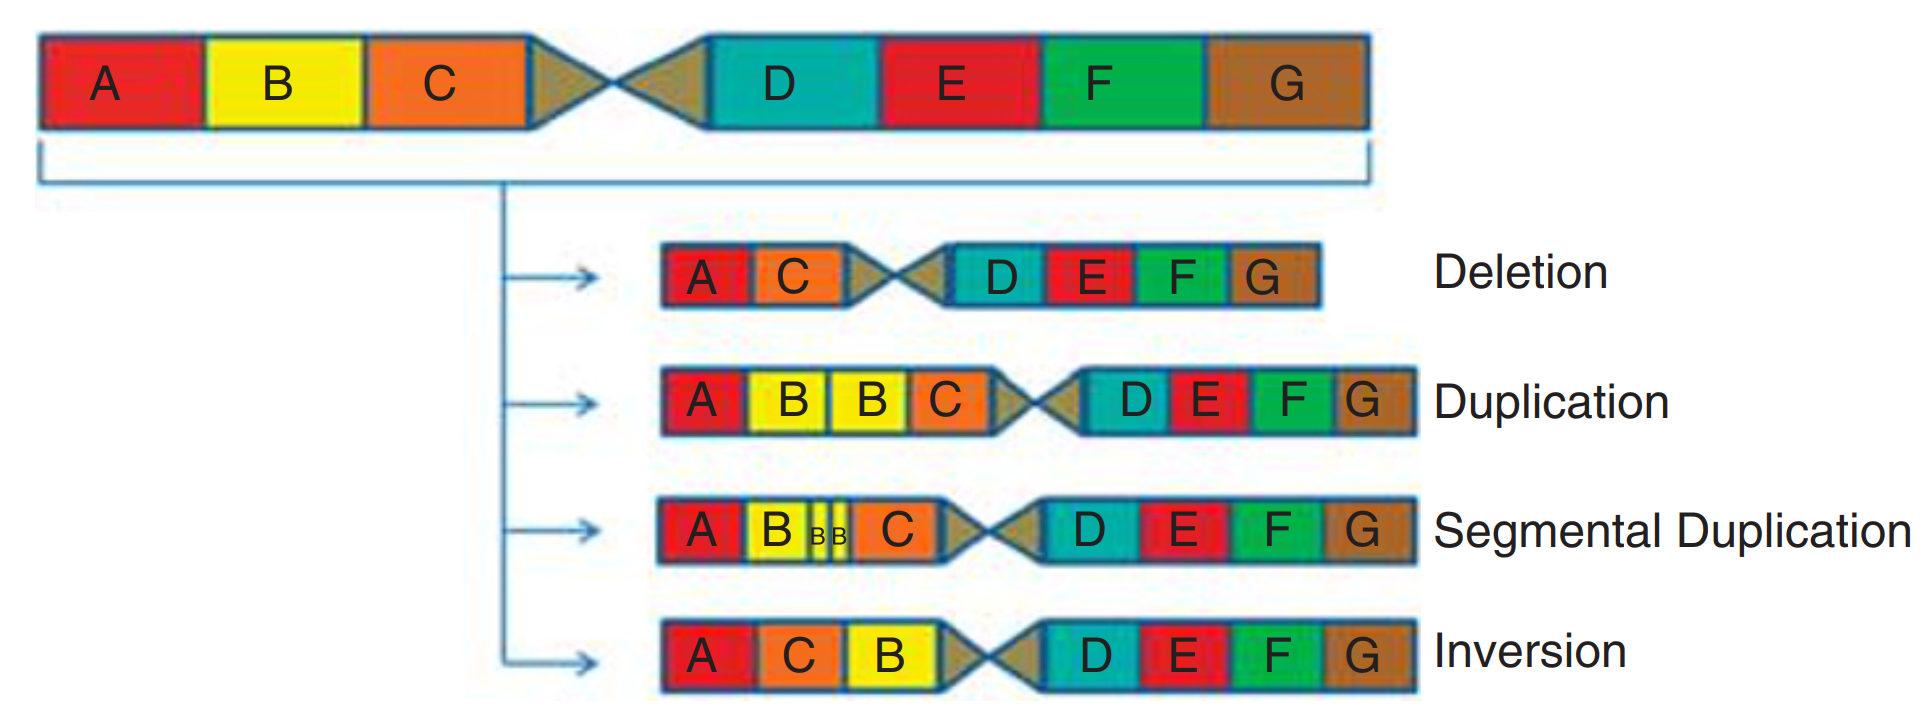
\includegraphics[scale=0.5]{images/cnv_v1.png} 
	\caption[Copy number variations, showing deletion, duplication, and inversion]{CNVs is classified into deletion, duplication, segmental duplication and inversion. These variations can affect an entire gene or a segment of a particular gene~\cite{almal2012implications}}	
	\label{fig:cnv_v1}
	\vspace{-2mm}
\end{figure*}

\hspace*{3.5mm} Besides, several biomarkers through single nucleotide polymorphisms~(SNP) studies have revealed an association with cancer and many other complex traits~\cite{almal2012implications}. An accurate identification of cancer based on CNVs can help to reveal the genetic predisposition for cancer before cancer actually occurs, so that vigilant prevention and rigorous monitoring may be practiced by those who are highly predisposed~\cite{19Cruz}. Inspired by this, CNVs were used to identify minimum redundancy maximum relevance feature selection and incremental feature selection methods~\cite{zhang2016classification} such that only one sample could be covered at a time or using microarray-based comparative genomic hybridization methods. Extracted CNVs features are then used to train machine learning~(ML) models for cancer identification, e.g., type prediction. Cancer typing methods based on manual feature selections and ML classifiers often involved inefficiency feature selection process using principal component analysis~(PCA) or recursive feature selection~\cite{malekpour2018mseq}. %, making them incapable for multiple samples and recurrent CNVs~\cite{malekpour2018mseq}. 

\hspace*{3.5mm} Nevertheless, genomics data, including CNVs, from TCGA show several characteristics~\cite{lu2003cancer} such as high dimensionality~(e.g., up to tens of thousands of genes), very small sample size~(e.g., less than $100$ samples), very sparse feature space~(e.g., as majority of genes are not responsible for cancer, making them irrelevant to cancer types classification). With such a huge feature space, even a robust ML model would fail to model the high-order non-linear interaction between biomarker genes. These characteristics make the overall analysis very challenging for  linear ML and tree-based models. ML-based approaches often fail to handle high dimensional and to model high-order interaction between a large number of biomarker genes. Besides, tree-based models are prone to overfitting, due to small sample size~\cite{lu2003cancer}. Since most genes are irrelevant for class distinction, their inclusion would not only introduce noise, but also trivial on-linearity~\cite{lu2003cancer}. Automated and robust feature selection and ranking of biologically meaningful biomarkers prior to classification help to mitigate these problems. 

\hspace*{3.5mm} In comparison with ML-based approaches, deep learning~(DL) approaches based on neural networks~(DNN), found to be effective. While convolutional neural networks~(CNN) is good at reducing frequency variations, long short-term memory~(LSTM) is good at modeling temporal and complex interactions between CNVs across genes. Further, a neural ensemble method is found to be more effective than structures solely based on CNN or LSTM. This chapter, focuses on CNVs-based cancer typing method~(i.e., single modality). We use MSeq-CNV~\cite{malekpour2018mseq} - a CNV feature extraction tool to extract recurrent CNVs~(i.e., including genomic deletions and duplication across samples). MSeq-CNV uses mixture density for modeling aberrations in depth of coverage and abnormalities in the mate pair insertion sizes. However, common CNVs across multiple samples can be detected. Since CNVs are very high dimensional, modelling non-linear interactions between oncogenes and protein-coding genes is very challenging. This chapter hypotheses the following to address above challenges: 

\begin{enumerate}[noitemsep]
    \item High dimensionality of genomic data\footnote{\textbf{H1}: Stacking and neural representation learning can be very effective at extracting most abstract features from high dimensional genomic data through a hierarchical learning process.} can be handled by learning most abstract features through a hierarchical learning process by stacking DNN architectures and neural representation learning. 
    \item A neural ensemble method\footnote{\textbf{H2}: A neural ensemble method by combining several deep architectures can be more effective than structures solely based on a single architecture by reducing generalization error}, by combining several deep architectures can be more effective than structures solely based on a single architecture by reducing generalization error.
\end{enumerate}

\hspace*{3.5mm} Based on these hypotheses, both {Conv-LSTM} and CAE networks were trained and evaluated separately. Predictions of multiple model snapshots are then combined based on model weighted averaging ensemble of the classifiers\footnote{Supporting publication: \textbf{Md. Rezaul Karim}, Stefan Decker, and Oya Beyan, ``A snapshot neural ensemble method for cancer type prediction based on copy number variations", \emph{Neural Computing and Applications}, November 30, 2019.}.  %Further, we provide interpretations about the prediction made by the neural network in order to make the cancer diagnosis more effective. 
The rest of the chapter is structured as follows:
\cref{chapter_3:rw} covers some related works concerning cancer diagnosis based on CNVs data and summarizes their potential limitations. \Cref{chapter_3:mm} chronicles the detail of the data collection and feature engineering before the network construction and training. \Cref{chapter_3:results} demonstrates some experimental results and discusses key findings of the study. \Cref{chapter_3:conclusion} provides explanations of the importance and relevance of the study reported, highlights potential limitations, and discuss some future works before concluding the chapter. 

\section{Related Work}\label{chapter_3:rw}
As shown in \cref{table:stateofart}, both genomic, bioimaging, and clinical outcomes~\cite{min} are used to provide accurate diagnosis. In particular, RNA-Seq data is more widely used to identify rare and common transcripts, isoforms, and non-coding RNAs in cancer. Single nucleotide polymorphism data used to identify segmental variations across multiple cancer genomes~\cite{82Tomczak,95Gaul}). Ning Z. et al.~\cite{zhang2016classification} used CNVs level from cBioPortal for Cancer Genomics\footnote{cBioPortal for Cancer Genomics: \url{https://www.cbioportal.org/}}~\cite{cerami2012cbio} to classify the patients into breasts, bladder urothelial, colon, glioblastoma, head and neck squamous cell, and kidney cancer types. They construct a dagging-based classifier where the feature space was reduced using minimum redundancy maximum relevance feature selection and incremental feature selection methods~\cite{zhang2016classification}. They achieved an accuracy of 75\%, indicating that mostly driver genes play key role in differentiating cancer types. 

\hspace*{3.5mm} Sanaa et al.~\cite{elsadek2018supervised} extended their work in which 7 ML classifiers were trained giving the random forest algorithm an accuracy of 86\%. Other works used omics data to identify various cancer types e.g., Fakoor et al.~\cite{fakoor} extract features from high dimensional GE data using PCA and classify them into acute myeloid leukemia, breast, and ovarian cancer patients. Besides, CNVs analysis based on different statistical methods also used to identify significant CN associated with different types of cancers~\cite{cancernet}. Fisher's exact test is applied on patient and control groups to identify copy numbers for hereditary breast and ovarian cancer~\cite{58Kuusisto}. Although Fisher's exact test is mainly used for CNV analysis~\cite{fish}, ML-based approaches are trending to improve the accuracy of cancer susceptibility, recurrence, and survival prediction~\cite{16Kourou}. However, accurate extraction of CNVs and dealing with dimensionality remain two key challenges. ML algorithms such as support vector machine~(SVM) and decision trees are found effect to extract the most significant CNVs features from high dimensional data. 

\hspace*{3.5mm} In comparison with ML-based approaches, recent DL techniques have shown more accurate and promising results for cancer identification in some studies. CNN is widely applied~\cite{19Cruz} on whole slide images in order to detect cancer regions with a very high degree of precision, which is mainly because CNN can extract deep features from different cohorts simultaneously. Ibrahim et al.~\cite{ibrahim} proposed a multilevel feature selection technique based on deep belief networks and unsupervised active learning from miRNA expression data, which outperforms PCA-based methods for hepatocellular and breast carcinoma identification. Danaee et al.~\cite{17Danaee} used stacked denoising autoencoder to extract features from the RNA-seq data, which are then fed into SVM and shallow neural network to classify the samples into malignant or benign tumor of breasts~\cite{18Chen}. DeepCNA is another CNN-based approach proposed by Yuan et al.~\cite{yuan2018cancer} for cancer type prediction based on CNVs and chromatin 3D structure. DeepCNA performs moderately well if both CNA and 3D chromatin structures are used in a multimodal setting, which is, however, not always possible in a resource constrained setting. % for genomics-based cancer detection. 

\hspace*{3.5mm} Besides, imaging modalities such as histology and radiological images are used for understanding the genetic and epigenetic causes of cancer~\cite{20Rajanna,23Zheng} and to identify the existence of cancer using CNN~\cite{19Cruz,xu}. GISTIC and mutation significance\footnote{MutSig and GISTIC provide statistical significance of recurrence of mutations and copy-number alterations in specific genes, URL: \url{https://software.broadinstitute.org/cancer/cga/mutsig}} tools were employed to analyse the samples, followed by K-means clustering to visualize genomic and transcription alterations in various cancers~\cite{wb}. X-ray and CRT images are also used, along with proteomic and genomic assays which shows success in cancer prediction and prognosis~\cite{28Zhou}. Often these images are used to generate noninvasive, functional, and molecular multispectral photoacoustic imaging to detect prostate cancer using K-means and SVM~\cite{23Zheng}. %Besides, histopathology images are used . 
%Literature~\cite{17Danaee} used stacked denoising autoencoder to extract features from RNA-seq data and then fed into SVM and shallow ANN to classify malignant or benign tumor of breasts~\cite{18Chen}. DeepCNA is another CNN-based approach for cancer type prediction based on CNVs and chromatin 3D structure~\cite{yuan2018cancer}.
%Apart from these works, restricted methods have been proposed based on CNVs for cancer risk and type predictions~\cite{ding2014application, zhang2016classification, elsadek2018supervised}. 

\begin{table*}[!ht]
    \caption{Different cancer detection methods, data types, and performance }
    \label{table:stateofart}
    \begin{center}
    \scriptsize
    \vspace{-6mm}
    \begin{tabular}{l|l|l|l|l|l}
        \hline
        \textbf{Reference} & \textbf{Approach} & \textbf{Cancer types} & \textbf{\#Sample} & \textbf{Data type} & \textbf{Accuracy} \\\hline
            Karim et al.~\cite{karim2018a2ic} & DBN/LSTM & 14 primary types & 15,699 & TCGA CNVs & 73\% \\\hline % 2018
            Yuan et al.~\cite{yuan2018cancer} & CNN & 25 primary types & 14,703 & CNA \& 3D cromatin & 90\% \\\hline % 2018
            Sanaa et al.~\cite{elsadek2018supervised} & LR & 6 primary types & 3,480  & CNVs & 85\% \\\hline % 2018
        	Cruz et al.~\cite{19Cruz} & CNN & Breast cancer  & 605 & Slide images & 96\%  \\\hline  % 2017
            Danee et al.~\cite{17Danaee} & MLP & Breast cancer & 1210 & RNA-seq & 94\% \\\hline % 2016
            Ning et al.~\cite{zhang2016classification} & Dagging & 6 primary types & 3,480  & CNVs & 75\% \\\hline % 2016
        	Rajana et al.~\cite{20Rajanna} & Deep NN & Prostate cancer & 807 & Histology & 95\%\\\hline
            Chen et al.~\cite{18Chen} & Shallow NN & Colon cancer  & 590 & Gene expression & 84\% \\ \hline % 2015
            Ahmed et al.~\cite{abdel2016breast} & DBN & Breast cancer & 569 & Wisconsin BRCA & 99\% \\ \hline % 2015
            Zheng et al.~\cite{23Zheng} & K-means/SVM & Breast cancer & 569 & Wisconsin BRCA & 97.38\% \\ \hline % 2014
            Xiaofan et al.~\cite{ding2014application} & Naïve Bayes & Cancer risk & 640 & Human SNP & 93\% \\ \hline % 2014
        \end{tabular}
        \vspace{-6mm}
    \end{center}
\end{table*}

\hspace*{3.5mm} Unlike conventional cancer typing methods that work on analyzing morphological appearances, gene expression~(GE) levels of the tumor cells are used to differentiate tumors that have similar histopathological appearances~\cite{paroder2006na+}. Different types of somatic mutations data such as point mutation, single nucleotide variation~(SNV), small insertion and deletion\footnote{These are commonly known as INDELs}, copy number aberration~(CNA), translocation, and CNVs are also used. Xiaofan D. et al~\cite{ding2014application} extracted recurrent CNVs from non-tumor blood cell DNA of healthy patients. They revealed key the difference between cancer patients and controls w.r.t copy number losses and gains. Although their study can predict cancer predisposition of unseen test groups of mixed DNA with high confidence, a has limited coverage of only Caucasian and Korean cohorts. 

%\hspace*{3.5mm} Imaging data such as histology and radiological images are used for understanding genetic and epigenetic causes in cancer analyses~\cite{yuan2018cancer,20Rajanna,23Zheng}. In particular, GISTIC, MutSig, and clustering algorithms are used to visualize genomic and transcription alterations in various cancers at an advanced level~\cite{wb}. X-ray and CRT images~\cite{25Cruz}, along with proteomic and genomic assays, are also used, which show great success in cancer prediction and prognosis~\cite{28Zhou}. These types of images are used to generate noninvasive, functional, and molecular imaging modality data called multispectral photoacoustic imaging~\cite{20Rajanna} in order to detect prostate cancer using K-means and SVM~\cite{23Zheng}. 

%\hspace*{3.5mm} Literature~\cite{17Danaee} used a stacked denoising autoencoder to extract features from the RNA-seq data, which are then feed into SVM and shallow ANN to classify malignant or benign tumor of breasts~\cite{18Chen}. DeepCNA is another CNN-based approach proposed for cancer type prediction based on CNVs and chromatin 3D structure with CNN~\cite{yuan2018cancer}. Although DeepCNA is very efficient in cases where both CNA and 3D chromatin structures are supplied, the availability of such resources is not always possible, like in genomics-based cancer detection. Therefore, many researchers try to extract genomics data to be consumed by the DNN architectures. Apart from these works, restricted approaches have been proposed based on CNVs for cancer risk and type predictions~\cite{ding2014application, zhang2016classification, elsadek2018supervised}. Xiaofan D. et al.~\cite{ding2014application} used recurrent CNVs from non-tumor blood cell DNAs of non-cancer subjects about hepatocellular carcinoma, gastric cancer, and colorectal cancer patients. They revealed the differences between cancer patients and controls with respect to CN losses and CN gains. Although their study can make predictions on the cancer predisposition of an unseen test group of mixed DNAs with high confidence, it was limited to only Caucasian and Korean cohorts. 

%\hspace*{3.5mm} Ning Z. et al.~\cite{zhang2016classification} used CNVs at a level of 23,082 genes for 2,916 instances from cBioPortal for Cancer Genomics to classify 6 different types of cancers, i.e., breasts, bladder urothelial, colon, glioblastoma, kidney, and head-and-neck squamous cell. They construct a dagging-based classifier in which the feature space was reduced into CNVs of 19 genes using mRMR and IFS methods. They managed to achieve an accuracy of 75\%, indicating that only a few genes may play important roles in differentiating cancer types. Sanaa et al.~\cite{elsadek2018supervised} used the same dataset and train 7 different classifiers in which random forest shows 86\% accuracy. %The data used the CNV in variant types of cancers were downloaded from the

\hspace*{3.5mm} These approaches have not only proven to be useful at improving cancer diagnosis and subsequent treatments, but also revealed subtype information~\cite{66Huang}. Inspired by this, we considered copy number segmentation an important feature in a previous approach~\cite{karim2018a2ic}, such that higher the segmentation mean, the higher the copy number would be in that region. The length of a copy number and its value were then calculated based on a difference between start and end positions of a CNV. We represented copy number loss and gain in terms of negative segmentation mean and positive segmentation mean, respectively. Copy number with segmentation values between a certain range were considered as noise and discarded from rest of the calculation. However, a manual approach for CNV extraction like this often fails to extract recurrent CNV features in the case of simultaneous analysis of multiple samples~\cite{malekpour2018mseq}. Consequently, MSeq-CNV is applied for more efficient extraction of CNVs. 

%\hspace*{3.5mm} %\subsection{Related works on multimodality}
%Literature~\cite{liang} proposed to cluster ovarian and breast cancer patients based on multiplatform genomics~(e.g. GE, DNA methylation, and miRNA expression) and clinical data. To deal with such multiplatform data, MAE is used in which latent features are extracted before clustering with the K-means. Ngiam et al.~\cite{NgiamKKNLN11} proposed a multimodal architecture to handle multimodality of audio and video features based on three methods: multimodal fusion, cross-modality learning, and shared representation learning. 
%While each method uses multimodalities on the feature learning steps, multimodal fusion uses multimodalities in supervised learning and testing. Cross-modality learning used one type of data for both supervised learning and validating, while shared representation learning used one kind of data for supervised learning and testing. The original idea behind the cross-modality learning is to handle multimedia objects where not all data have all modalities. Liang et al.~\cite{liang} adopts a similar architecture for clustering multimodal cancer genomics GE, DNA methylation, and clinical data.

\section{Methods}\label{chapter_3:mm}
In this section, we discuss in detail the data collection, preprocessing, and feature engineering. % in detail. %, followed by the preparation of training, validation, and test sets. 

\subsection{Problem statement}
A CNV sample $x$ consists of a set of $m$ attribute-value pairs $\left(a_{i}, v_{i}\right)$, where $a_i$ is a feature and $v_i$ is its value from $a_{i}$, where both $a_{i}$ and $v_i \in \mathbb{R}^{D}$. %From given $n$ CNV samples $X$ = ${\{x_1,x_2, ..., x_n}\}$ in dataset $D$, where $x \in \mathbb{R}^{D}$. 
Let $X_{1}, X_{2}, \ldots, X_{m}$ be the CNV samples~(independent $m$-dimensional CNV samples~(i.e., $m$ is number of genes)) for the respective genes $G_{1}, G_{2}, \ldots, G_{m}$ respectively, where $X_{i} \in \mathbb{R}^{D}$ $\operatorname{dom}\left(X_{i}\right)$ which is the range of copy numbers for gene $G_{i}$. Let $C$ be the random variable for the class labels, and $\operatorname{dom}(C)=\{1, \ldots, K\},$ where $K$ denotes the total number of classes. If $t=\left\{t . X_{1}, t . X_{2}, \ldots, t . X_{m}\right\}$ denotes a size $m$ tuple of copy numbers for $m$ genes, $T=$ $\left\{\left(t_{1}, c_{1}\right),\left(t_{2}, c_{2}\right), \ldots,\left(t_{n}, c_{n}\right)\right\}$ denotes a training set of $n$ tuples, where $i=\{1,2, \ldots, n\}, c_{i} \in \operatorname{dom}(C)$ is the class label of tuple $t_{i} 
%Let the test set be $S=\left\{t_{1}, t_{2}, \ldots, t_{l}\right\}$ where $l$ is the size of the test set A classifier is a function Class with two arguments, $T$ and $s,$ where $T$ denotes the training samples and $s$ is a testing sample. Function Class returns a class prediction for sample $s .$ The classification accuracy is defined as the number of correct predictions made by the classifier on a set of testing tuples.
%Given a training set $T=\left\{\left(t_{1}, c_{1}\right),\left(t_{2}, c_{2}\right), \ldots,\left(t_{n}, c_{n}\right)\right\},$ where 
%$t_{i}$ are independent $m$-dimensional GE values~(i.e., $m$ is number of genes), 
=\left(t_{i} \cdot X_{1}, t_{i} \cdot X_{2}, \ldots, t_{i} \cdot X_{m}\right), m \gg n$ and $c_{i} \in \operatorname{dom}(\mathrm{C})$ is the class label of the $i^{th}$ tuple. 
First, we extract important features based on oncogenes and non-coding human genes. 
Then we consider classifying an individual $x$ into a specific group or cancer type, where a predictor~(e.g., a classifier) is a function $F: {X}^{(m)} \rightarrow {Y}$, which maps the data instance from a feature space ${X}^{(m)}$ with $m$ input features to a labels $y$ in a target space ${Y}$, where $F(x)=y$ denotes the decision $y$, predicted by $F$. We also assume that $F$ is a `black-box' predictor, whose internal functioning is either unknown~(or partially known) or known but not interpretable by a human. 
 
%In \cref{chapter:uni_modality}, we developed a `black-box' predictor $f$ whose internal functioning is either unknown~(or partially known) to the observer or they are known but not interpretable by a human. In this chapter, instead we denote $\widetilde{f}$- an interpretable predictor, whose internal processing yielding a decision $\widetilde{f}(x)=y$ can be given a symbolic interpretation understandable by a human. %Examples of such predictors include rule-based classifiers, decision trees, decision sets, and rational functions. 

%the classifier $f$ maps an input $x$ to an output $f(x) \in y, f: \mathbb{R}^{d} \mapsto y$.

\subsection{Datasets}
\label{data}
Copy numbers and gene coordinates of different cancer types from TCGA are used in our study, which are hybridized by genome sequencing technology called {affymetrix SNP 6.0}, which allows us to examine the largest number of cases along with the highest probe density~\cite{31Park}. Tumor tissue and healthy tissue samples are collected from each cancer patient, which are curated from the blood, bone marrow, Buccal cell, EBV immortalized, and solid tissues. For consistency across samples, all data were downloaded from the same platform but with different project ID and gender. However, blood-derived healthy samples of only 14 cancer types were downloaded having at least 400 samples, as shown in~\cref{table:alldatadetails}. 

\begin{table} [!ht]
    \small
    \caption{Number of CNV samples across 14 different tumor types used in this chapter}
    \vspace{-2mm}
    \label{table:alldatadetails}
    \centering{
    \begin{tabular}{l|l|l|l}
        \hline
        \rowcolor{Gray}
         \textbf{Cohort} & \textbf{\#Tumor sample} & \textbf{\#Healthy sample} & \textbf{Carcinoma type} \\\hline
        COAD & 502 & 468 & Colon cdenocarcinoma \\\hline
        GBM  & 609 & 527 & Glioblastoma multiforme \\\hline
        KIRC & 586 & 530 & Kidney renal clear cell carcinoma  \\\hline
        LGG  & 514 & 487 & Brain lower grade glioma \\\hline
        LUAD & 554 & 591 & Lung adenocarcinoma \\\hline
        LUSC & 524 & 535 & Lung squamous cell carcinoma \\\hline
        OV   & 572 & 546 & Ovarian serous cystadenocarcinoma \\\hline
        UCEC & 548 & 545 & Uterine corpus endometrial carcinoma \\\hline
        BRCA & 1103 & 1103 & Breast invasive carcinoma  \\\hline 
        HNSC & 519 & 562 & Head \& neck squamous cell carcinoma \\\hline 
        THCA & 505 & 513 & Thyroid carcinoma \\\hline 
        PRAD & 501 & 536 & Prostate adenocarcinoma \\\hline 
        STAD & 442 & 464 & Stomach adenocarcinoma \\\hline 
        BLCA & 416 & 397 & Bladder urothelial carcinoma \\\hline
    \end{tabular}}
    \vspace{-2mm}
\end{table}

\iffalse
\begin{table} [h]
\centering
    \scriptsize
    \caption{number of CNV samples across 14 different tumor types}
    \label{table:alldatadetails}
    \vspace{-2mm}
    \begin{tabular}{l|l|l|l}
        \hline
        \rowcolor{Gray}
         \textbf{Cohort} & \textbf{DNA methylation} & \textbf{Copy numbers} & \textbf{Mutations} & \textbf{miRNA} & \textbf{Gene expression} & \textbf{Carcinoma type} \\\hline
            LUSC & 358 & 345 & 178 & 332 & 227 & Lung squamous cell carcinoma \\\hline
            READ & 162 & 164 & 69 & 143 & 71 & Rectum adeno-carcinoma \\%
            GBM  & 405 & 578 & 290 & 501 & 495 & Glioblastoma multiforme \\\hline
            LAML & 194 & 198 & 197 & 187 & 179 & Acute myeloid leukemia	\\%
            HNSC & 310 & 310 & 277 & 309 & 303 & Head \& neck squamous cell carcinoma \\\hline 
            BLCA & 126 & 126 & 99 & 121 & 96 & Bladder urothelial carcinoma \\\hline 
            KIRC & 457 & 457 & 417 & 442 & 431 & Kidney renal clear cell carcinoma  \\\hline
            UCEC & 512 & 511 & 248 & 497 & 333 & Uterine corpus endometrial carcinoma \\\hline
            LUAD & 431 & 357 & 229 & 365 & 355 & Lung adenocarcinoma \\\hline
            OV   & 592 & 577 & 316 & 454 & 581 & Ovarian serous cystadenocarcinoma \\\hline
            BRCA & 888 & 887 & 772 & 870 & 817 & Breast invasive carcinoma  \\\hline
            COAD & 420 & 422 & 155 & 407 & 192 & Colon cdenocarcinoma \\\hline
            %LGG  & 514 & 487 & Brain lower grade glioma \\\hline
            %THCA & 505 & 513 & Thyroid carcinoma \\\hline 
            %PRAD & 501 & 536 & Prostate adenocarcinoma \\\hline 
            %STAD & 442 & 464 & Stomach adenocarcinoma \\\hline 
    \end{tabular}
\end{table}

\fi 

\hspace*{3.5mm} We consider gender an important feature for cancer subtype classification, since tumors such as {BRCA} and {OV} are not common in males, whereas {PRAD} is only common in males. TCGA do not specify if a sample is curated from healthy tissue or tumor tissue, so we downloaded CNV files in separate groups. Each cancer sample is then grouped as primary and blood-derived samples during filtering before dividing them into male and female groups. We also used gene locations in combination with the copy number data, which are available in all patients for each tumor under each TCGA project. Gene coordinates were collected from cytobands using the ensemble library of \texttt{biomaRt} package\footnote{\url{https://www.ensembl.org/biomart}}. Additionally, oncogenes information were downloaded\footnote{TCGA has listed 568 oncogenes till September 2017} from the TCGA portal. 
%An example of a raw sample of GBM tumor is given in \cref{cnv:gbmCNV2}. 
%Each row in the table represents copy number changes at a specific DNA segment. For example, there is a copy number gain in the first row, which is from location 61,735 to 28,43676 in chromosome 1. However, only 557 probes being used to identify this segment change, which is quantified to 0.0548. Negative segment change represents the deletion from that region. 

\hspace*{3.5mm} Initial prepossessing were required to remove noise, empty, or string values from both CNV and gene data. For each cancer type, samples were downloaded into four different groups: healthy samples from male, healthy samples from female, tumor samples from male, and tumor samples from female. Then we preprocessed CNV data for 15,699 separate samples. Then, all the cancer samples and healthy tissue samples were combined. We found that the distribution of copy numbers across tumor samples are very different. For example, BRCA has almost double the samples of most other tumors. Whereas, {STAD} and {BLCA} have fewer samples compared to other tumor samples except for those having samples between 500-600. While, more than 400 THCA samples have 50 to 100 CNVs per sample, and around 50 OV tumor samples have less than 200 CNVs per sample. 

\iffalse
\begin{table} [!ht]
    \vspace{-3mm} 
    \caption{Example of a COAD CNV sample after preprocessing}
    \label{sample:afterpreprocessing}
    \begin{center}
    \small
    \begin{tabular}{l|l|l|l|l|l|l|l}
    \hline
    \rowcolor{Gray}
    \textbf{Chr} & \textbf{Start} & \textbf{End} & \textbf{Length} & \textbf{Segment\_Mean} & \textbf{Gain/Loss} & \textbf{Gender} & \textbf{Type} \\\hline
        1 & 1710664 & 1741164 & 30500 & -1.2237 & 0 & 0 & 1 \\\hline
    	1 &	16577231 &	16637050 &	59819  & 0.4852 &	1 &	0 &	1  \\\hline
    	1 &	16684955 &	16721910 &	36955  & 0.7576 &	1 &	0 &	1  \\\hline
        1 &	16721984 &	16855942 &	133958   & -0.5558 &	0 &	0 &	1  \\\hline 
    \end{tabular}
    \end{center}
    \vspace{-3mm}
\end{table}
\fi 

\hspace*{3.5mm} Although, most tumor samples have copy numbers between 50-400, there are a few samples having more than 1,500, giving on average 226.80 copy numbers per sample. On average, 106.92 copy numbers exist per healthy sample, which is less than half of tumor samples. Usually, healthy human cells have very different copy numbers in terms of location, length, and number and vary in humans. This makes the CNVs of the human genome an utterly complex and dynamic structure. For a cancer-affected patient, this structure becomes even more complex and dynamic as the tumor grows. In general, healthy human cells have completely different copy numbers in terms of location, length, and number from another human. 

\hspace*{3.5mm} We solve this dynamic dimension problem by using gene locations of the human genome since DL models expect fixed dimension inputs only. We selected a fixed number of genes and extracted the copy numbers that overlapped with the gene locations, removing them from the protein non-coding gene because arguably more than 80\% of human genes do not encode any protein. Thus, copy numbers from these regions have little-to-no effect on tumor growth. %By using gene locations, we safely removed copy numbers that fall within non-coding regions and kept those copy numbers that only affect genes.
%In addition, since not all genes are available in every human body and vary from person to person, genes are also variable in the human genome. 
We prepared two different datasets of CNVs based on oncogenes and protein-coding genes that are used to train the Conv-LSTM and CAE networks to get the ensemble from. Additionally, some preprocessed data\footnote{Based on a Master thesis I co-supervised with Dr. Oya Beyan: "Using Deep Neural Networks and Copy Number Variations for Cancer Detection", by Md. Ashiqur Rahman, Software Systems Engineering, RWTH Aachen University, 2018.} were reused. %Data co %\Cref{fig:pipeline} shows the overall processing pipeline of our proposed approach.

\subsection{Feature selection from protein-coding genes}
We used the CNVs of 20,308 protein non-coding genes. Since not all of these genes are responsible for tumor growth, features from irrelevant genes make the CNV data unnecessarily complex. Neural networks then fail to converge the training, resulting in poor performance. Although using protein-encoding genes makes the dimension fixed, 95\% of the features will be empty across the samples (e.g., a sample with 500 CNVs has 19,808 empty features making empty features for 19,808 cases). Using gene locations adds two additional complexities evolved: the curse of dimensionality and sparsity. 

\hspace*{3.5mm} To solve these problems, we perform CNV analysis in combination with 568 oncogenes responsible for the majority of cancer types. While oncogenes are found to be related to tumor growth, it is not confirmed which other genes also responsible for its growth. In such a setting, consecutive genes with non-zero values represent copy number length, and negative or positive segmentation values represent loss and gain, respectively. We hypothesize that DNN will be able to identify those hidden non-linear features. 

\subsection{Feature selection from oncogenes}
There are structural variations in DNA where protein-encoding genes are not present, and these genes have no effect on tumor growth. One way to remove such unnecessary segments is by keeping only those copy numbers that fall within gene regions and discarding the rest using oncogenes, because oncogenes not only control the cell division but are also responsible for gene expression changes due to external or natural causes and could lead to the development of tumor at some point. Thus, by considering only 568 oncogenes, we prepared another CNV representation instead of taking the whole 20,308 genes. 

\hspace*{3.5mm} As stated earlier, the manual CNV feature extraction is not efficient, and the recurrent CNVs from multiple samples are often ignored, we used the MSeq-CNV tool, which is an efficient CNV extraction method. In order to model the number of mate pairs with aberration in the insertion size and Poisson distribution for emitting the read counts, MSeq-CNV applies the binomial distribution-based mixture density on each genomic position. This applies a mixture density for modeling aberrations in depth of coverage and abnormalities in the mate pair insertion sizes. After applying MSeq-CNV, genome-wide copy gain and loss regions are saved in a matrix form, where each row represents a different CNV call with its sample number, start position, end position, and copy number estimation.
 
 \iffalse
\begin{figure}[ht!]
    \centering
    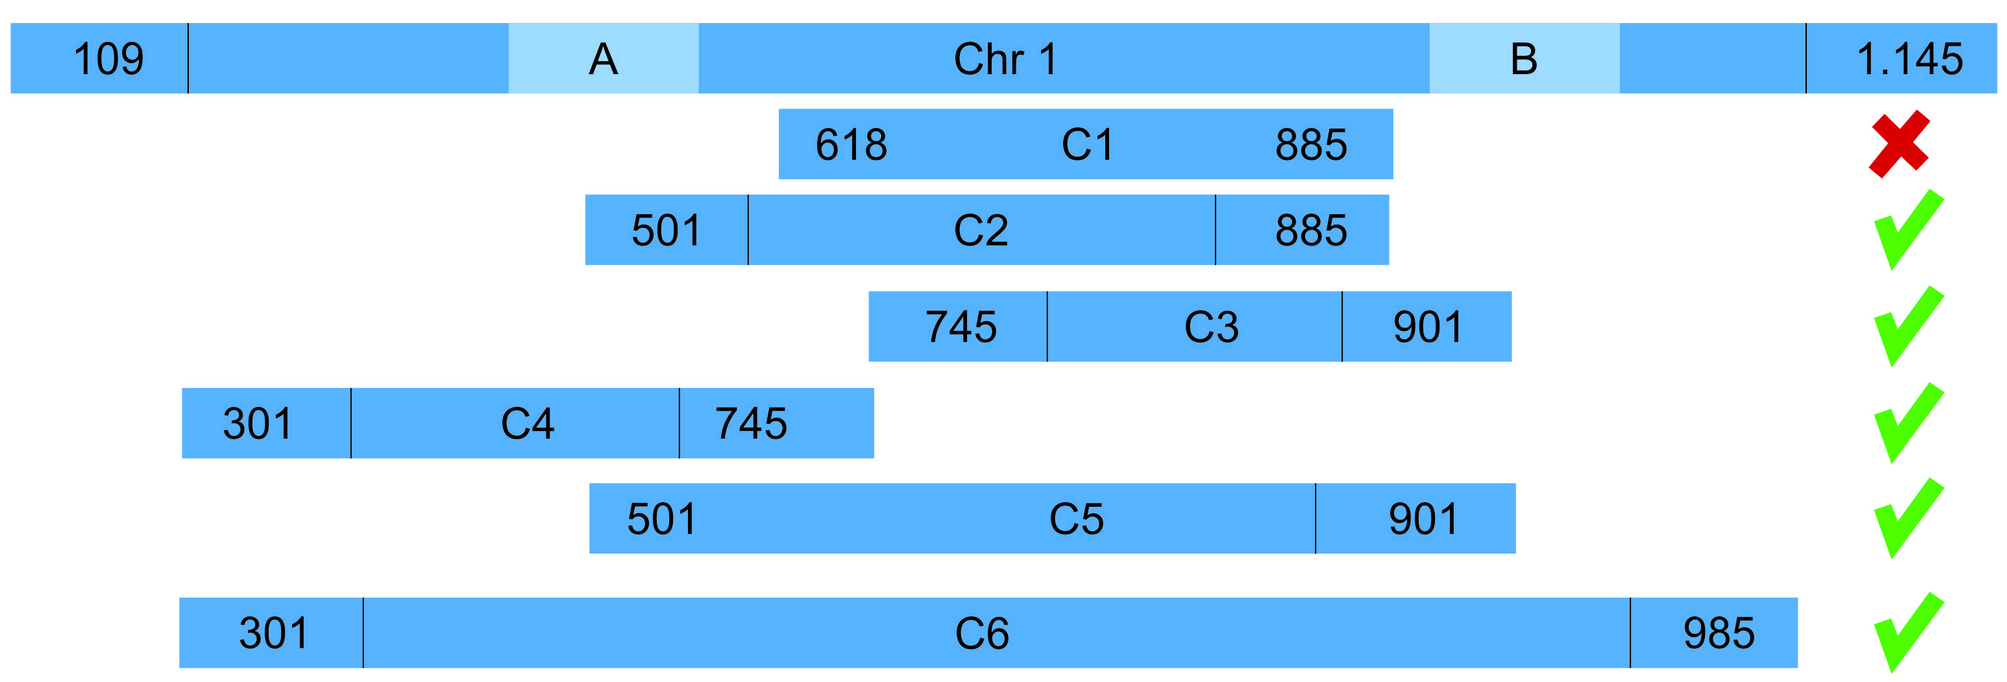
\includegraphics[width=0.90\textwidth,height=55mm]{images/fe.png}
    \caption{CNV selection process using MSeq-CNV}
    \label{fig:cnv_overlap}
\end{figure}
\fi 

%An example of the CNV selection process is shown in \cref{fig:cnv_overlap}. It shows a reference segment of chromosome 1 at the top that extends from DNA location 109 to 1,145 with two genes, A and B, within this segmental region. Below this reference, there are six candidate copy numbers~(C1-C6) at this location. C1 is a candidate copy number that extends between genes A and B, but C1 does not overlap with any one of them, which is why we remove it from the calculation. Candidates C2 and C3 are copy numbers, too, which slightly overlap with A and B, respectively. We still consider them as valid copy numbers because gene positions are not always fixed. C4 and C5 both fully overlap with genes A and B, hence, they are also valid copy numbers. C6 is not only a big segmental copy number, but it also overlaps with both genes. However, since we consider only the part of genes that overlap, we discard rest of the regions from the calculation. This is based on the hypothesis that even if a candidate copy number overlaps with a gene just by one base pair, we still consider it as a valid copy number~\cite{CNV2}. 

\vspace{-2mm}
\begin{table} [!ht]
    \caption{Example of training data prepared based CNVs representation of oncogenes}
    \label{cnv:changed232d}
    \vspace{-6mm}
    \begin{center}
        \scriptsize
        \begin{tabular}{l|l|l|l|l|l|l|l}
            \hline
            \rowcolor{Gray}
            \textbf{Type} & \textbf{Gender} & \textbf{PRDM16} & \textbf{RPL22} & \textbf{CAMTA1} & \textbf{MTOR} & .. & \textbf{MTCP1} \\\hline    
            COAD & 1 & -0.3195 & -0.2154 & 0 & 0.4767  & .. & 0.652 \\\hline
            PRAD & 0 & 0.230 & -0.552 & 1.715 & -0.92  & .. & -1.0 \\\hline
            OV & 1 & -1.240 & 0.975 & 0.350 & 0.642  & .. & 0.985 \\\hline
        \end{tabular}
        \vspace{-6mm}
    \end{center}
\end{table}
\vspace{-3mm}

\hspace*{3.5mm} Each gene has a starting and ending position in DNA, which is similar for copy numbers having starting and ending positions. For each gene, MSeq-CNV checks if a sample has any CNV region overlaps with that gene. Then it assigns the segment value for that gene, otherwise 0 is assigned. This means that a tumor sample has different copy number variation than a reference, which is measured by the segment value. If the value is positive, copy number in that gene is considered to be more increased than the reference. A negative value, however, signifies that the gene was deleted from that DNA location. A sample of the final training data is shown in table \ref{cnv:changed232d}. The first row shows a male patient's GBM tumor sample, where gene PRDM16 and RPL22 have copy number losses with segmentation values of 0.3195 and 0.2154, respectively. Whereas, gene CAMTA1 has no copy number variation, and so on. %Eventually, dimension of the training set reduced from 20,308 to 568 (+ the label column). 

\subsection{Network construction and training}
\label{nc}
We construct and train Conv-LSTM and CAE networks on two different CNVs representations~(i.e., oncogenes and protein-coding genes), followed by the creation of multiple snapshot models. Then we evaluate each network independently, followed by the MEA to combine the snapshot models. 

\subsubsection{Construction of Conv-LSTM network }
We construct and train the Conv-LSTM network by combining both CNN and LSTM layers as shown in \cref{fig:conv_lstm}. While the CNN model uses conv filters to capture local relationship values, an LSTM network can carry overall relationship of a whole CNV sequence more efficiently. This turns Conv-LSTM into a powerful architecture to capture long-term dependencies between features extracted by CNN~\cite{karim2019drug}. To capture both the local and global relationships, all the input ${X}_{1},{X}_{2},...,{X}_{t}$ cells in Conv-LSTM output ${C}_{1},{C}_{2},...,{C}_{t}$, hidden states ${H}_{1},{H}_{2},....,{H}_{t}$, and gates $i_t$,$f_t$,$o_t$ of the network as 3D tensors whose last two dimensions are spatial dimensions. %To get a better picture of the inputs and states, we may imagine them as vectors standing on a spatial grid. 
Conv-LSTM determines the future state of a certain cell in the input hyperspace by the inputs and past states of its local neighbors, which is achieved by using a convolution operator in the state-to-state and input-to-state transitions, which can be represented as follows~\cite{Conv_LSTM1,karimACCA2019}:

\vspace{-4mm}
\begin{align}
    \begin{array}{c}
            {i_{t}=\sigma\left(W_{x i} * {X}_{t}+W_{h i} * {H}_{t-1}+W_{c i} \circ {C}_{t-1}+b_{i}\right)} \\
            {f_{t}=\sigma\left(W_{x f} * {X}_{t}+W_{h f} * {H}_{t-1}+W_{c f} \circ {C}_{t-1}+b_{f}\right)} \\
            {{C}_{t}=f_{t} \circ {C}_{t-1}+i_{t} \circ \tanh \left(W_{x c} * {X}_{t}+W_{c o} * {C}_{t}+b_{o}\right)} \\
            {\qquad {H}_{t}=o_{t} \circ \tanh \left({C}_{t}\right)}
    \end{array}
\end{align}
\vspace{-4mm}

\hspace*{3.5mm} In the above equation,~`*'~denotes the conv operator and `o' is the entrywise multiplication of two matrices of same dimensions. The second LSTM layer emits an output `H', which is then reshaped into a feature sequence and feeds into fully connected layers to predict the cancer types at the next step and as an input at the next time step. Intuitively, an LSTM layer treats an input feature space as timesteps and outputs arbitrary hidden units per timestep. On the other hand, once the input feature space is passed to the conv layer, we pad the input such that the output has the same length as the original input. 

\begin{figure*}
	\centering
	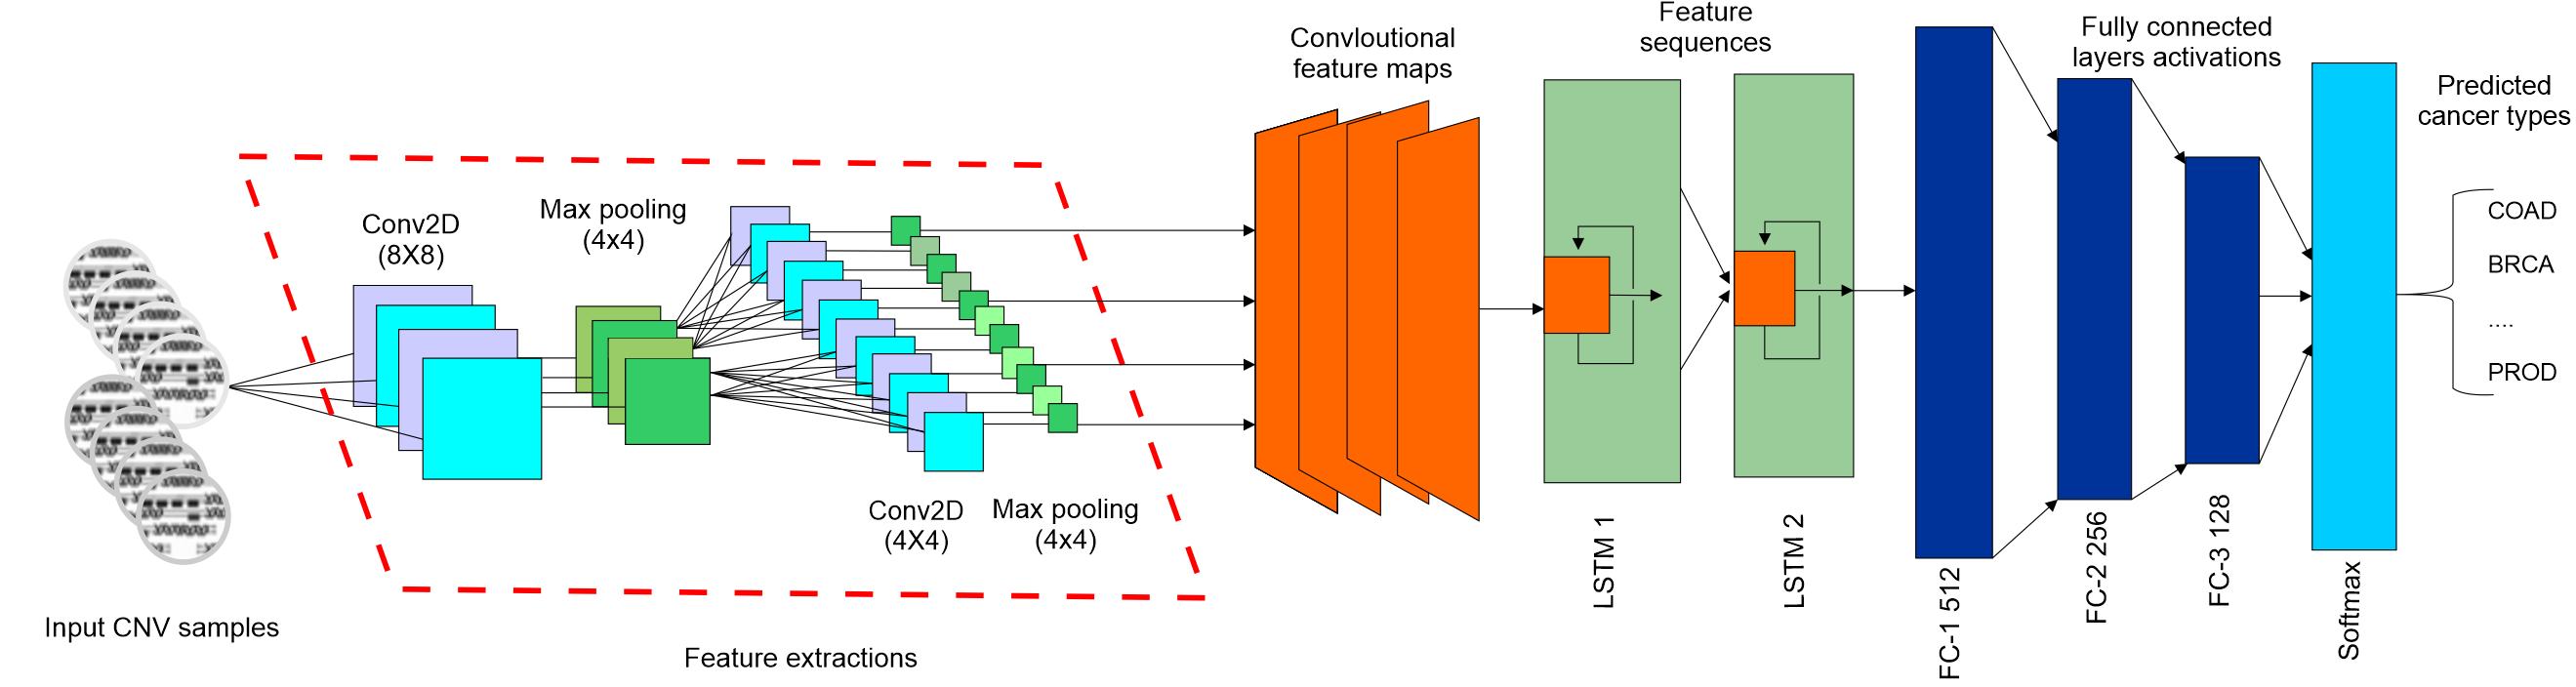
\includegraphics[scale=0.5]{images/conv_lstm.png} 
	\caption[Schematic representation of the convolutional-LSTM network]{Schematic representation of the Conv-LSTM network starts from taking input CNV samples and passing to CNN layers before getting a sequence vector representation from the LSTM layers to pass to dense, dropout, and softmax layers~\cite{karimACCA2019}}	
	\label{fig:conv_lstm}
	\vspace{-2mm}
\end{figure*}

\hspace*{3.5mm} Output of each conv layer is then passed to the dropout layer to regularize learning to avoid overfitting~\cite{vardropout}. To down sample the input feature space into lower dimensional representation, two max pooling layer~(MPL) are placed with different filter size. The output of an MPL can be considered as an `extracted feature' from each CNV samples. Since each MPL follows to `flatten' the output space by taking the highest value in each timestep dimension, this helps produce a sequence vector, e.g., feature sequence from the last LSTM layer, which help the network to learn abstract features~(w.r.t. driver genes) that are highly indicative of being responsible for specific cancer type. This vector is then fed into the neural network  through another dropout and the softmax layers for the probability distribution over the classes. 

\subsubsection{Construction of CAE classifier}
Using the Conv-LSTM-based network, we have seen how to extract both local and globally important features for classifying individual samples from a limited number of labelled samples. However, in cases of very small numbers of training samples, unsupervised pretraining has proven highly effective~\cite{ae1,ae2,ae3}. 
%\subsubsection{Handling data sparsity}
Humans communicate through languages or signs, which is analogous to biological organisms too, that convey information within and between cells through information encoded in biological sequences~\cite{yue2018deep}. To understand the language of life unsupervised data-driven representation learning methods such as BioVec~\cite{asgari2015continuous} is proposed. BioVec embeds biological sequences in lower dimensional vector space to characterizes biophysical and biochemical properties of sequences, and is already proven effective~\cite{yue2018deep}. 

\begin{figure*}[h]
	\centering
	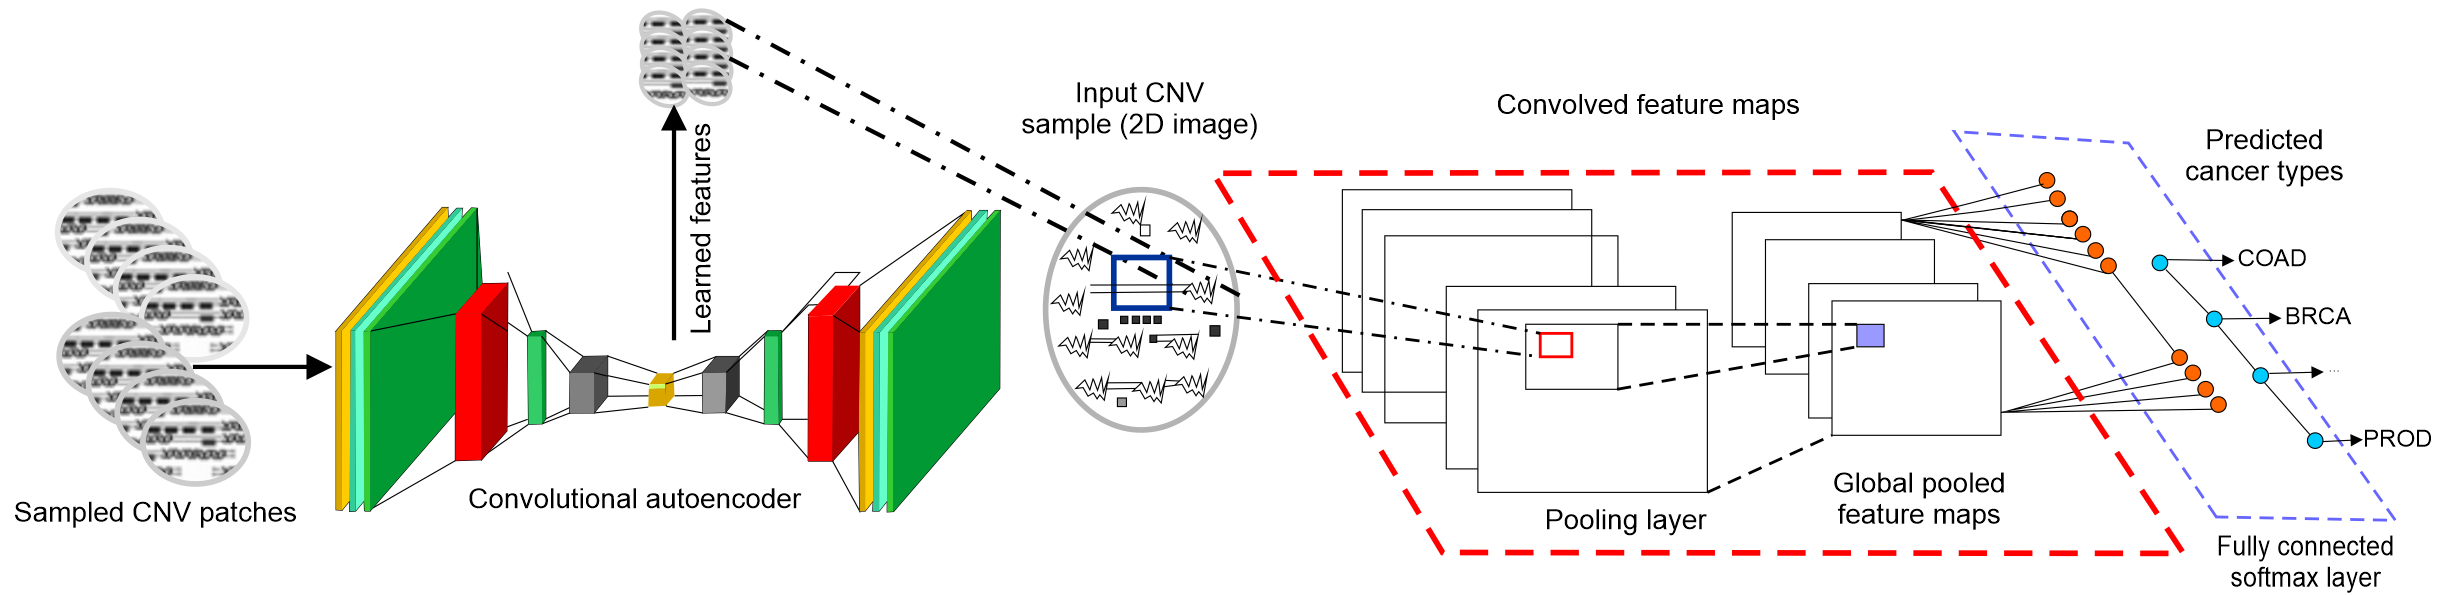
\includegraphics[scale=0.6]{images/cae.png}	
    \caption{Schematic representation of the CAE classifier~\cite{karimACCA2019}}
	\label{fig:cae}
\end{figure*}


\hspace*{3.5mm} Further, since both datasets are very sparse,  CAE-based representation learning is employed. Since sparse AEs are intrinsically sparse, it is important to apply sparsity constraints, e.g., self-regularization, with all the typical benefits associated with sparsity: it forces the model to focus on the really important features, highly reducing the risk of overfitting~\cite{karimBIB2019}. Especially, it is a major methodological guide for the correct tuning of the model capacity, progressively augmenting it to attain sparsity, or conversely reducing the dimension of the network removing links to zeroed out neurons~\cite{sparseAE}. 

\hspace*{3.5mm} Due to the sparsity of $L_1$ regularization, sparse AEs actually learns better representations such that the activation are sparser, which makes it perform better than an a regular AE without $L_1$ regularization as an AE learns latent representations instead of redundant information in our input data. 
%\subsubsection{CAE network construction}
We constructed a CAE, which is architecturally a 19-layer autoencoder, in which a batch normalization layer is used after every convolutional layer and the ReLu activation function in every layer except for last layer that uses a Softmax activation function. From the given CNV samples, feature map is calculated using convolutional layer in the encoder module. The pooling layer is calculated by down-sampling the convolutional layer by taking the maximum value in each non-overlapping sub-region. The CAE classifier contains of two parts: i) the CAE autoencoder and ii) the classifier. The CAE autoencoder part has the following structure: 

\begin{enumerate}[noitemsep]
    \scriptsize{
        \item Input layer: each CNVs sample is reshaped from 1 x 20,736 to 144 x 144
        \item Convolutional layer: of size 32 x 20,736 (i.e. 144 x 144) 
        \item Batch normalization layer: of size 32 x 20,736
        \item Convolutional layer: of size 32 x 20,736
        \item Batch normalization layer: of size 32 x 10,368
        \item Max-pooling layer: of size 32 x 10,368
        \item Convolutional layer: of size 64 x 10,368
        \item Batch normalization layer: of size 64 x 10,368
        \item Convolutional layer: of size 64 x 10,368
        \item Batch normalization layer: of size 64 x 10,368
        \item Convolutional layer: of size 128 x 10,368
        \item Batch normalization layer: of size 128 x 10,368
        \item Convolutional layer: of size 128 x 10,368
        \item Batch normalization layer: of size 128 x 10,368
        \item Convolutional layer: of size 128 x 10,368
        \item Batch normalization layer: of size 128 x 10,368
        \item Convolutional layer: of size 64 x 10,368
        \item Batch normalization layer: of size 64 x 10,368
        \item Upsampling layer: of size 64 x 20,736 
        \item Convolutional layer: of size 1 x 20,736.}
\end{enumerate}

\hspace*{3.5mm} After training the CAE, we remove the decoder components by making the first 19 layers trainable false\footnote{Since the encoder part is already trained}. On top of these components, we add a flattening layer, followed by a fully connected dense layer of size 128, followed by a Softmax output unit of 14, i.e., the number of classes. 

\subsection{Network training and neural ensemble} %all human genes
Each of Conv-LSTM and CAE is trained in two steps. Training is performed independently, followed by creating their multiple snapshots before applying MAE. Network parameters are initialized with Xavier initialization~\cite{xavier} and trained using AdaGrad - a first-order gradient-based optimization technique to optimize the categorical cross-entropy loss as: 

\vspace{-2mm}
\begin{equation} 
    E_{c} = \sum_{i, j, k} T_{i, j, k} \log P_{i, j, k}+\left(1-T_{i, j, k}\right) \log \left(1-P_{i, j, k}\right)
    \label{eq:cce3}
\end{equation} 

\begin{figure*}
    \centering
    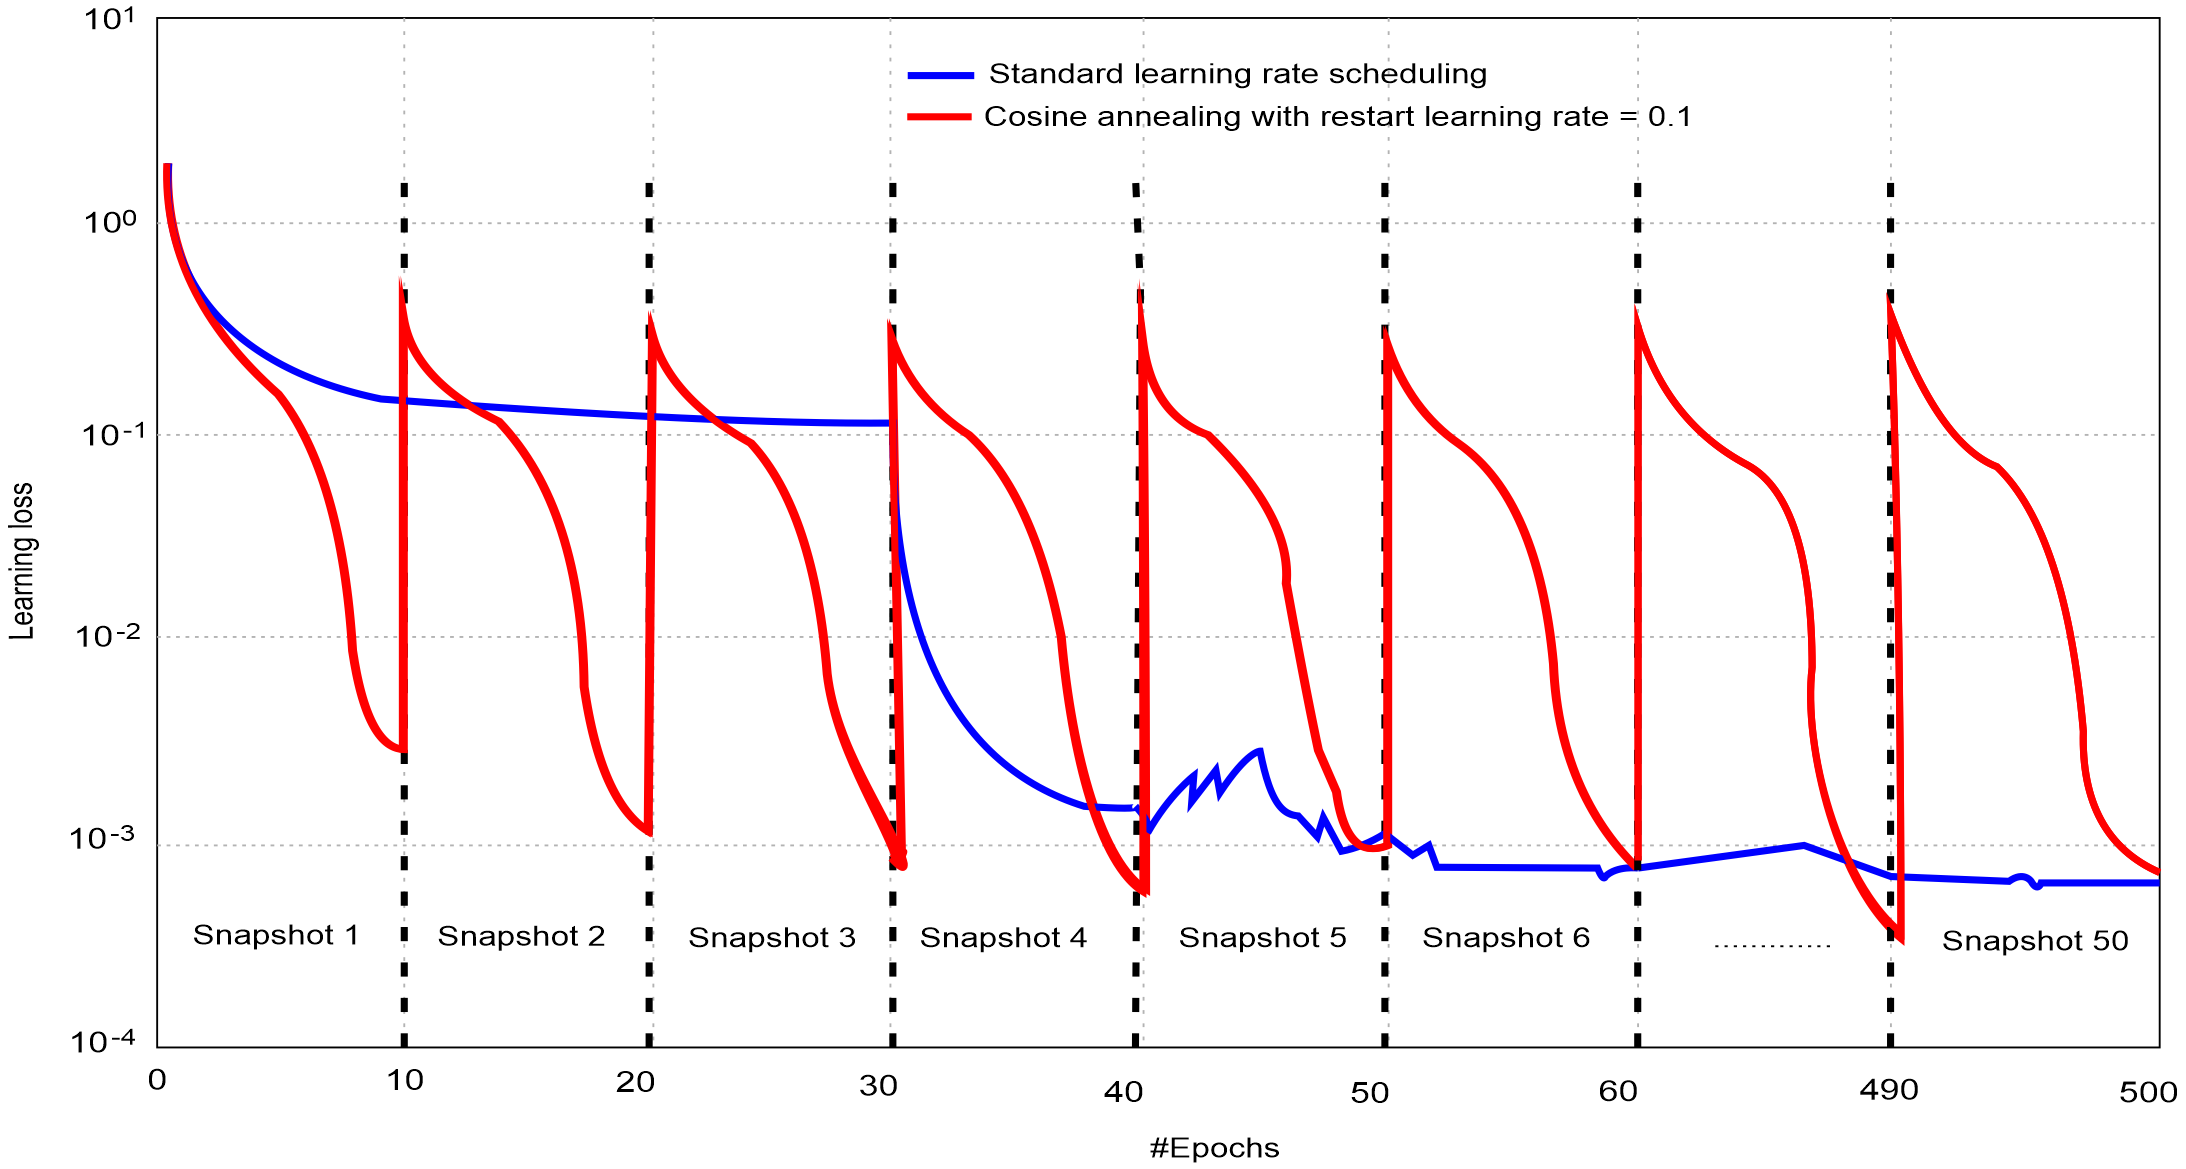
\includegraphics[scale=0.55]{images/cac.png}
    \caption[Cosine cyclic annealing-based training]{Training loss of Conv-LSTM network with standard learning rate~(blue) vs. cosine annealing~(red). The intermediate models~(denoted by the dotted lines) form an ensemble at the end of training~\cite{karimACCA2019}}
    \label{fig:ca}
    \vspace{-2mm}
\end{figure*}

\hspace*{3.5mm} Softmax activation function is used in the output layer for the probability distribution over the classes. Hyperparameters are defined in grid search and 10-fold cross-validation by varying learning rates and different batch sizes. Further, Gaussian noise layers are added, followed by convolutional and LSTM layers to improve model generalization and to reduce overfitting. 
%Model ensemble technique helps the neural network to achieve improved performance compared to the predictions from a single model by reducing the generalization error. 
%We hypothesize\footnote{\textbf{$H_3$:} A neural ensemble method, combining several deep architectures, can be more effective than structures solely based on a single model by reducing the generalization error~\cite{karimACCA2019}.} that a neural ensemble method by combining several deep architectures can be more effective than structures solely based on a single model~\cite{karimACCA2019}.
Cyclic cosine annealing~(CCA) is employed. CCA  aggressively~(but systematically) changes the learning rate~(LR) over epochs to produce different network weights~\cite{loshchilov2016sgdr}. Multiple model snapshots are created during a single training run and combine the predictions to make an ensemble prediction \cite{huang2017snapshot}. 

\hspace*{3.5mm} CCA requires total training epochs, maximum learning rate, and number of cycles, as well as the current epoch number making the initial LR and the total number of training epochs as two hyperparameters. Hence, CCA will have an effect of starting with a large LR, which is relatively rapidly decreased to a minimum value before being dramatically increased again to the following LR for the given epoch~\cite{huang2017snapshot}. CCA aggressively but systematically changes the learning rate over training epochs to produce very different network weights~\cite{loshchilov2016sgdr}, as outlined in~\cref{fig:ca}. 

\begin{equation}
    \label{eq:lr-cosine}
    \alpha(t)=\frac{\alpha_{0}}{2}\left(\cos \left(\frac{\pi \bmod (t-1,\lceil T / M\rceil)}{\lceil T / M\rceil}\right)+1\right)
\end{equation}

\begin{figure}
    \centering
        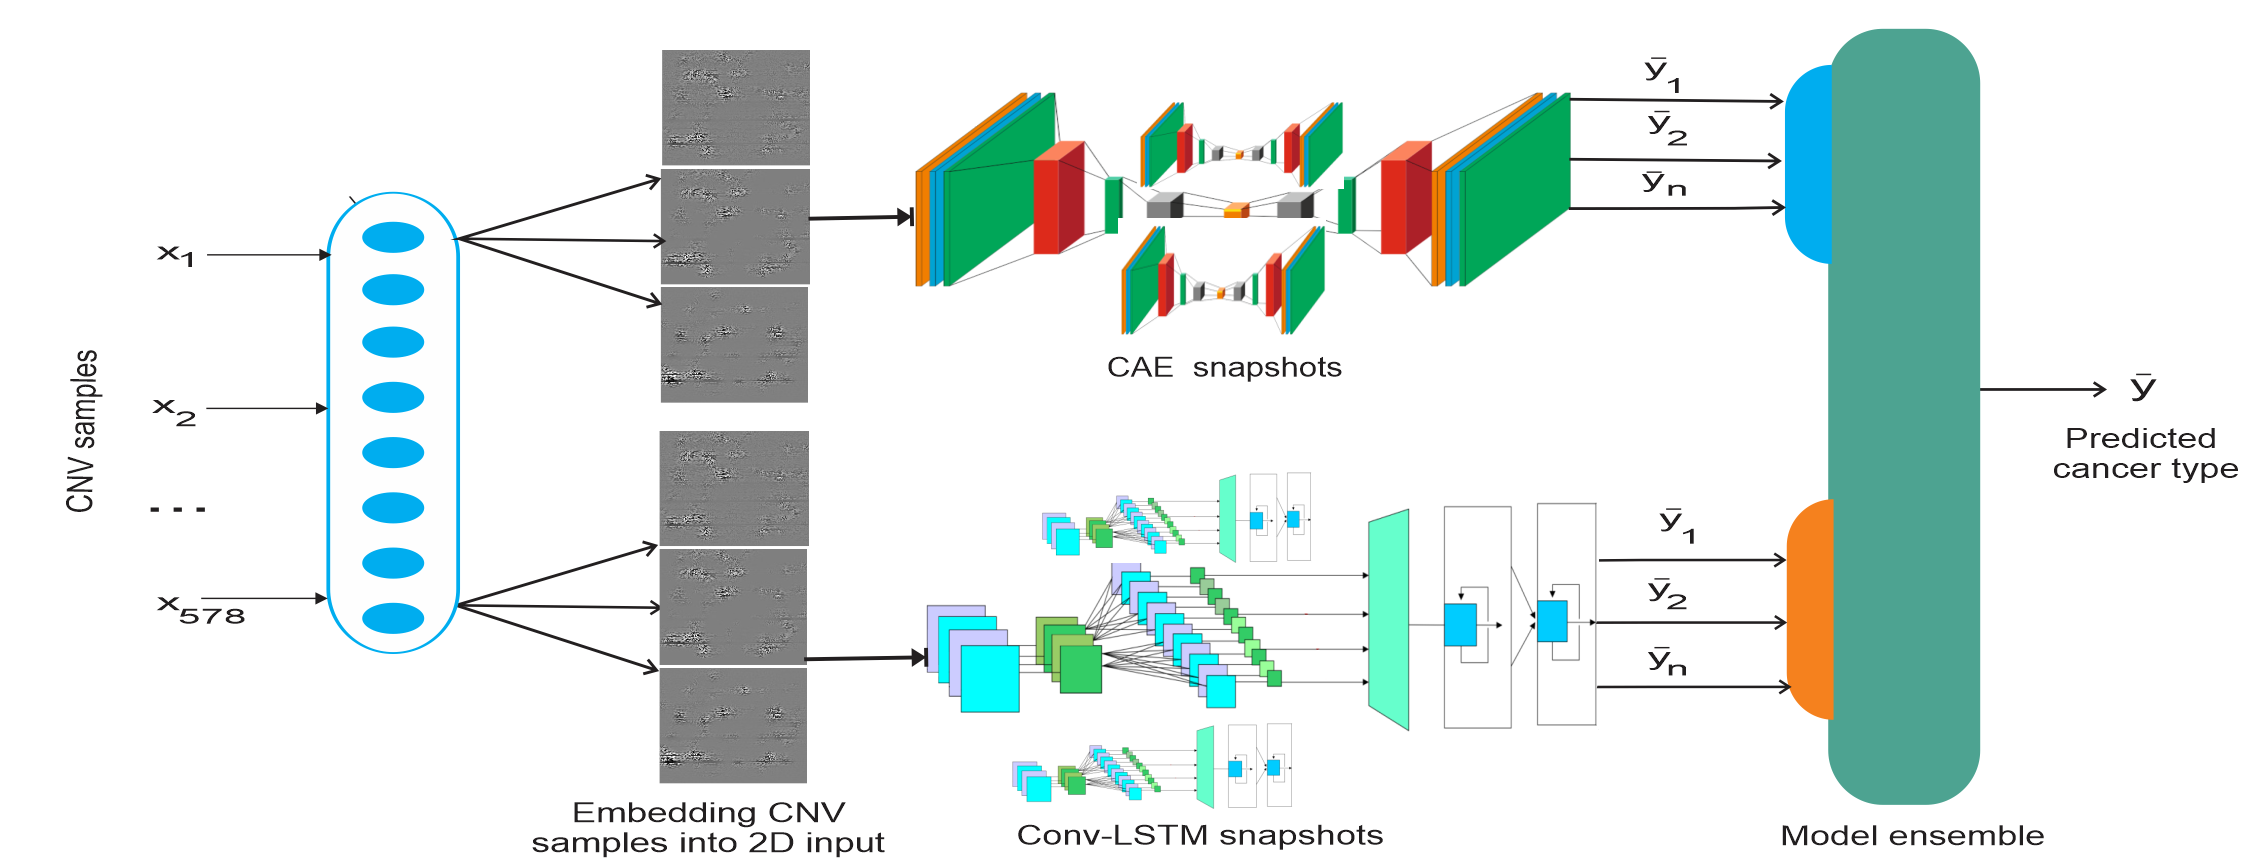
\includegraphics[scale=0.65]{images/ensemble.png}
    \caption{Model averaging ensemble of Conv-LSTM and CAE snapshots~\cite{karimACCA2019}}
    \label{fig:mae}
    \vspace{-2mm}
\end{figure}

\hspace*{3.5mm} In \cref{eq:lr-cosine}, $\alpha(t)$ is the LR at epoch t, $\alpha_0$ is the maximum LR, $T$ is the total epoch, $M$ is the number of cycles, $mod$ is the modulo operation, and square brackets indicate floor operations. During the training of the ensemble model, we set total epochs, maximum learning rate, number of cycles, and current epoch number. Initial learning rate and total number of epochs are treated as hyperparameters. After training, best weights at the bottom of each cycle are saved as the snapshot of each model for $M$ cycles, giving $M$ model snapshots. Network undergoes several LR annealing cycles, converging to and escaping from multiple local minima during snapshot ensembling. The ensemble prediction is computed at test time, by averaging last $m$ model's Softmax outputs, where $m \leq M$, where $\mathbf{x}$ is a test sample and $h_i \left(\mathbf{x} \right)$ is the softmax score of snapshot $i$, the final output is the simple mean of the last $m$ models as follows~\cite{huang2017snapshot}: 

\vspace{-2mm}
\begin{equation}
    h_{\mathrm{MAE}}=\frac{1}{m} \sum_{0}^{m-1} h_{M-i}(\mathrm{x})
    \label{eq:mae}
\end{equation}

\hspace*{3.5mm} Finally, all the snapshots are collected and used in the final ensemble using MEA as shown in \cref{fig:mae}. Although, each model's weights are subjected to dramatic changes during training for the subsequent LR cycles, CCA allows the learning algorithm to converge to a different solution. Subsequently, the ensemble model gives the lowest test error~\cite{huang2017snapshot}. %, since an exhaustive optimization would be too computationally expensive. %Further, we only use a single object property to test how results change with each choice of parameter, due to computational constraints. 

\section{Experiments}\label{chapter_3:results}
We carried out several experiments based on protein-coding genes and oncogenes. By using each network and CNV representation, cancer type predictions were experimented separately. The results of each experiment with a comparative analysis will be discussed in detail in this section. 

\subsection{Experiment setup}
We perform the hyperparameter optimization through a random search and 5-fold cross-validation tests. First, we optimize the parameters for the individual model, followed by the optimization of the ensemble model. During the training of Conv-LSTM and CAE, 70\% of the data is used for the training, 30\% for the evaluation, and 10\% from the training set to optimize the learning rate, batch size, number of filters, kernel size, dropout probability, and Gaussian noise probability. For pretraining the CAE, 90\% of data is used for the training, and 10\% of the data is used for validation. 

\hspace*{3.5mm} During the ensemble training, number of epochs~(NE), maximum learning rate, and number of cycles~(NC), are set to 500, 1.0, and NE/10, respectively, for each model for 50 cycles through a grid search, giving 50 snapshots. We report macro-averaged precision and recall as classes are imbalanced. We do not report F1-scores since it is significant only when the value of precision and recall are very different. Further, for cancer diagnosis, it is important to have both high precision and recall. Hence, results with very different precision and recall are not useful in cancer diagnosing and tumor type identification. The MAE is then followed to report the final predictions. 

\subsection{Performance analysis of individual models}
Classification accuracies using oncogenes and all non-coding genes vary. In particular, using protein-coding genes, classifiers perform moderately well, giving accuracies of 72.96\% and 76.77\% with Conv-LSTM and CAE network, respectively. Since classes are imbalanced, accuracy alone gives distorted estimation of the cancer types. Thus, class-specific classification reports are shown in \cref{table:codingene} and \cref{table:resultoncogene}. As shown in~\cref{table:codingene}, precision and recall for majority cancer types were moderately high in which CAE performed mostly better than Conv-LSTM network. In particular, CAE classifier can classify COAD, GBM, KIRC, BRCA, LUSC, and PRAD more confidently~(at least 82.50\% of the cases); Conv-LSTM classified the OV tumor samples more accurately than CAE classifier~(83.56\% vs 76.13\%). 

\begin{table} [h]
\caption{Performance on cancer type prediction using non-coding genes}
\label{table:codingene} %RF Confusion Matrix all genes Subtype
    \begin{center}
        \vspace{-5mm}
    \scriptsize
        \begin{tabular}{l|ll|ll|l}
        \hline
        \rowcolor{Gray}
        {} & \multicolumn{2}{c}{\textbf{Conv-LSTM~(72.96\%)}} & \multicolumn{2}{c}{\textbf{CAE~(76.77\%)}} &  {} \\\hline
        \textbf{Tumor type} & \textbf{Precision} &  \textbf{Recall}  & \textbf{Precision} &  \textbf{Recall} & \textbf{Support} \\\hline
        COAD    & 0.6981  &  0.7325 & 0.7924 &    0.8250 & 133  \\\hline
        GBM     & 0.8127  &  0.8275 & 0.8247 &   0.8765  & 151  \\\hline
        KIRC    & 0.8013  &  0.7335 & 0.8331 &   0.8468  & 150  \\\hline
        LGG     & 0.8250  &  0.6935 & 0.8642 &   0.7835 & 120  \\\hline
        LUAD    & 0.6835  &  0.6584 & 0.6992 &   0.7238 & 136  \\\hline
        LUSC    & 0.6937  &  0.7294 & 0.7438 &   0.8352 & 132  \\\hline
        OV      & 0.7539  &  0.8356 & 0.8365 &   0.7613 & 145  \\\hline
        UCEC    & 0.6645  &  0.6829 & 0.7435 &   0.6834 & 131  \\\hline
        BRCA    & 0.7357  &  0.7587 & 0.7954 &   0.8386 & 269  \\\hline
        HNSC    & 0.7134  &  0.7235 & 0.6853 &   0.7542 & 141  \\\hline
        THCA    & 0.6967 &  0.6959 & 0.7025 &   0.7654 & 121  \\\hline
        PRAD    & 0.7225  &  0.7934 & 0.8395 &   0.8345 & 124  \\\hline
        STAD    & 0.6528  &  0.6917 & 0.6776 &   0.6512 & 113  \\\hline
        BLCA    & 0.7356  &  0.6589 & 0.7925 &   0.7489 & 108  \\\hline
        \rowcolor{LightCyan}
        \textbf{Avg/total} & \textbf{0.7278} &    \textbf{0.7296} & \textbf{0.7593} &    \textbf{0.7677} & \textbf{1974}  \\\hline
        \end{tabular}
        \vspace{-4mm}
    \end{center}
\end{table}

\hspace*{3.5mm} The downside is that both classifiers have made a substantial amount of mistakes e.g., CAE can classify STAD and UCEC tumor cases only 65\% and 68\% accurately; Conv-LSTM network made more mistakes particularly for the STAD, BLCA, THCA, UCEC, LUAD, and LGG tumor samples. On the other hand, although the tumor-specific classification accuracies varied across classes, the overall accuracies increased moderately and reached 74.25\% and 78.32\% using Conv-LSTM and CAE, respectively. As seen in~\cref{table:resultoncogene}, the precision and recall for most of the cancer types are higher than that of protein-coding gene-based CNVs. Similar to the previous experiment, CAE performed mostly better than the Conv-LSTM network across tumor types. In particular, CAE classifier can correctly classify COAD, GBM, OV, UCEC, PRAD, and BLCA in at least 80\% of the cases showing higher confidence. 

\begin{figure}[h]
	\centering
	\begin{subfigure}{0.48\linewidth}
		\centering
		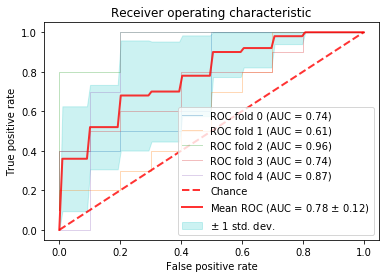
\includegraphics[scale=0.55]{images/download1.png}
		\caption{Using CAE classifier}
	\end{subfigure}
	\hspace{2mm}
	\begin{subfigure}{0.48\linewidth}
		\centering
		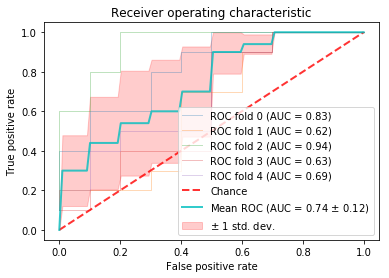
\includegraphics[scale=0.55]{images/download2.png}
		\caption{Using Conv-LSTM network}
	\end{subfigure}
	\caption{The ROC curves for Conv-LSTM and CAE models across folds} 
	\label{fig:roc}
	 \vspace{-2mm}
\end{figure}

\begin{table}[h]
\caption{Performance on cancer type prediction using oncogenes }
\label{table:resultoncogene} 
\begin{center}
    \scriptsize
    \vspace{-5mm}
    \begin{tabular}{l|ll|ll|l}
        \hline
        \rowcolor{Gray}
        {} & \multicolumn{2}{c}{\textbf{Conv-LSTM (74.67\%)}} & \multicolumn{2}{c}{\textbf{CAE (78.32\%)}} &  {} \\\hline
        \textbf{Tumor type }& \textbf{Precision} &  \textbf{Recall}  & \textbf{Precision} &  \textbf{Recall} & \textbf{Support~(CAE)} \\\hline
        COAD   & 0.7785 & 0.7564 & 0.8265 & 0.8193 & 133  \\\hline
        GBM    & 0.8254 & 0.8330 & 0.8433 & 0.8524 & 151  \\\hline
        KIRC   & 0.7753 & 0.7835 & 0.8172 & 0.8035 & 150  \\\hline
        LGG    & 0.8235 & 0.7136 & 0.7976 & 0.8031 & 120  \\\hline
        LUAD   & 0.7520 & 0.7351 & 0.7584 & 0.7674 & 136  \\\hline
        LUSC   & 0.7528 & 0.6475 & 0.7139 & 0.7256 & 132  \\\hline
        OV     & 0.8327 & 0.8407 & 0.8665 & 0.8538 & 145  \\\hline
        UCEC   & 0.7726 & 0.7625 & 0.8732 & 0.8412 & 131  \\\hline
        BRCA   & 0.7956 & 0.8075 & 0.8012 & 0.7965 & 269  \\\hline
        HNSC   & 0.8253 & 0.6932 & 0.7025 & 0.6929 & 141  \\\hline
        THCA   & 0.7953 & 0.8025 & 0.7429 & 0.7581 & 121  \\\hline
        PRAD   & 0.8267 & 0.8237 & 0.8781 & 0.8626 & 124  \\\hline
        STAD   & 0.7924 & 0.6945 & 0.7632 & 0.7737 & 113  \\\hline
        BLCA   & 0.8368 & 0.7979 & 0.8623 & 0.8553 & 108  \\\hline
        \rowcolor{LightCyan}
        \textbf{Avg/total} &   \textbf{0.7543}    &  \textbf{0.7467} &    \textbf{0.7945}   &  \textbf{0.7832} & \textbf{1974} \\\hline
    \end{tabular}
     \vspace{-6mm}
    \end{center}
\end{table}

\hspace*{3.5mm} On the contrary, Conv-LSTM classified the BRCA and THCA tumor samples more accurately than the CAE classifier. The downside is that both classifiers have made substantial mistakes, too. For example, CAE could classify HNSC and LUSC tumor samples accurately in only 69\% and 72\% of the cases. Whereas, the Conv-LSTM network made more mistakes, particularly for the STAD, HNSC, LUSC, and LGG tumor samples. In summary, both classifiers performed moderately well except for certain types of tumor cases such as STAD, HNSC, BLCA, THCA, UCEC, LUAD, LUSC, and LGG. The ROC curves in \cref{fig:roc} based on CNVs from oncogene shows that AUC scores generated by both the Conv-LSTM model and CAE classifier are consistent across folds, and AUC scores generated by the CAE classifier are about 4\% better than that of the Conv-LSTM network.

\begin{figure}[h]
	\centering
	\begin{subfigure}{0.48\linewidth}
		\centering
		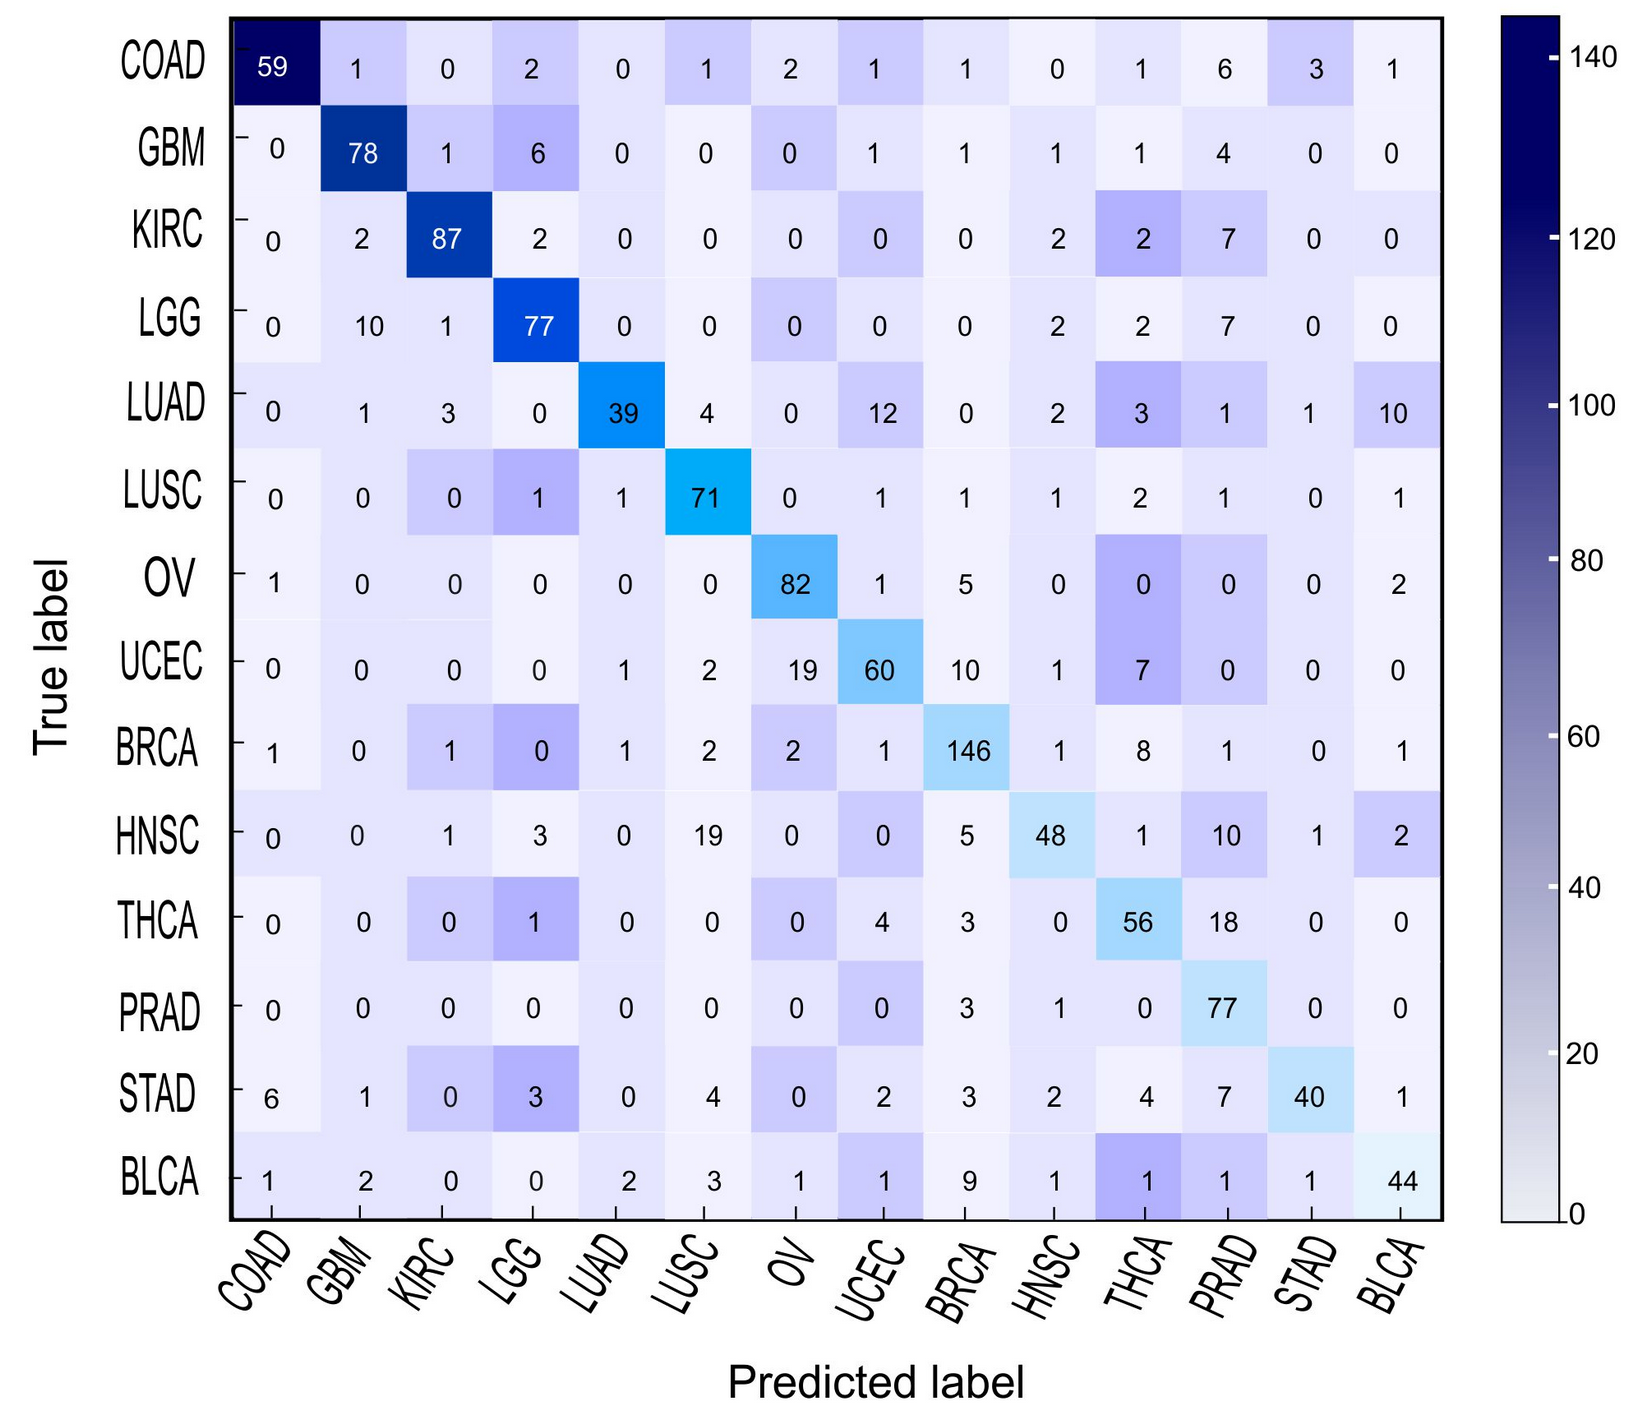
\includegraphics[scale=0.35]{images/cm1.png}
		\caption{Using coding genes based CNVs}
        \label{fig:cm_1}
	\end{subfigure}
	\hspace{2mm}
	\begin{subfigure}{0.48\linewidth}
		\centering
		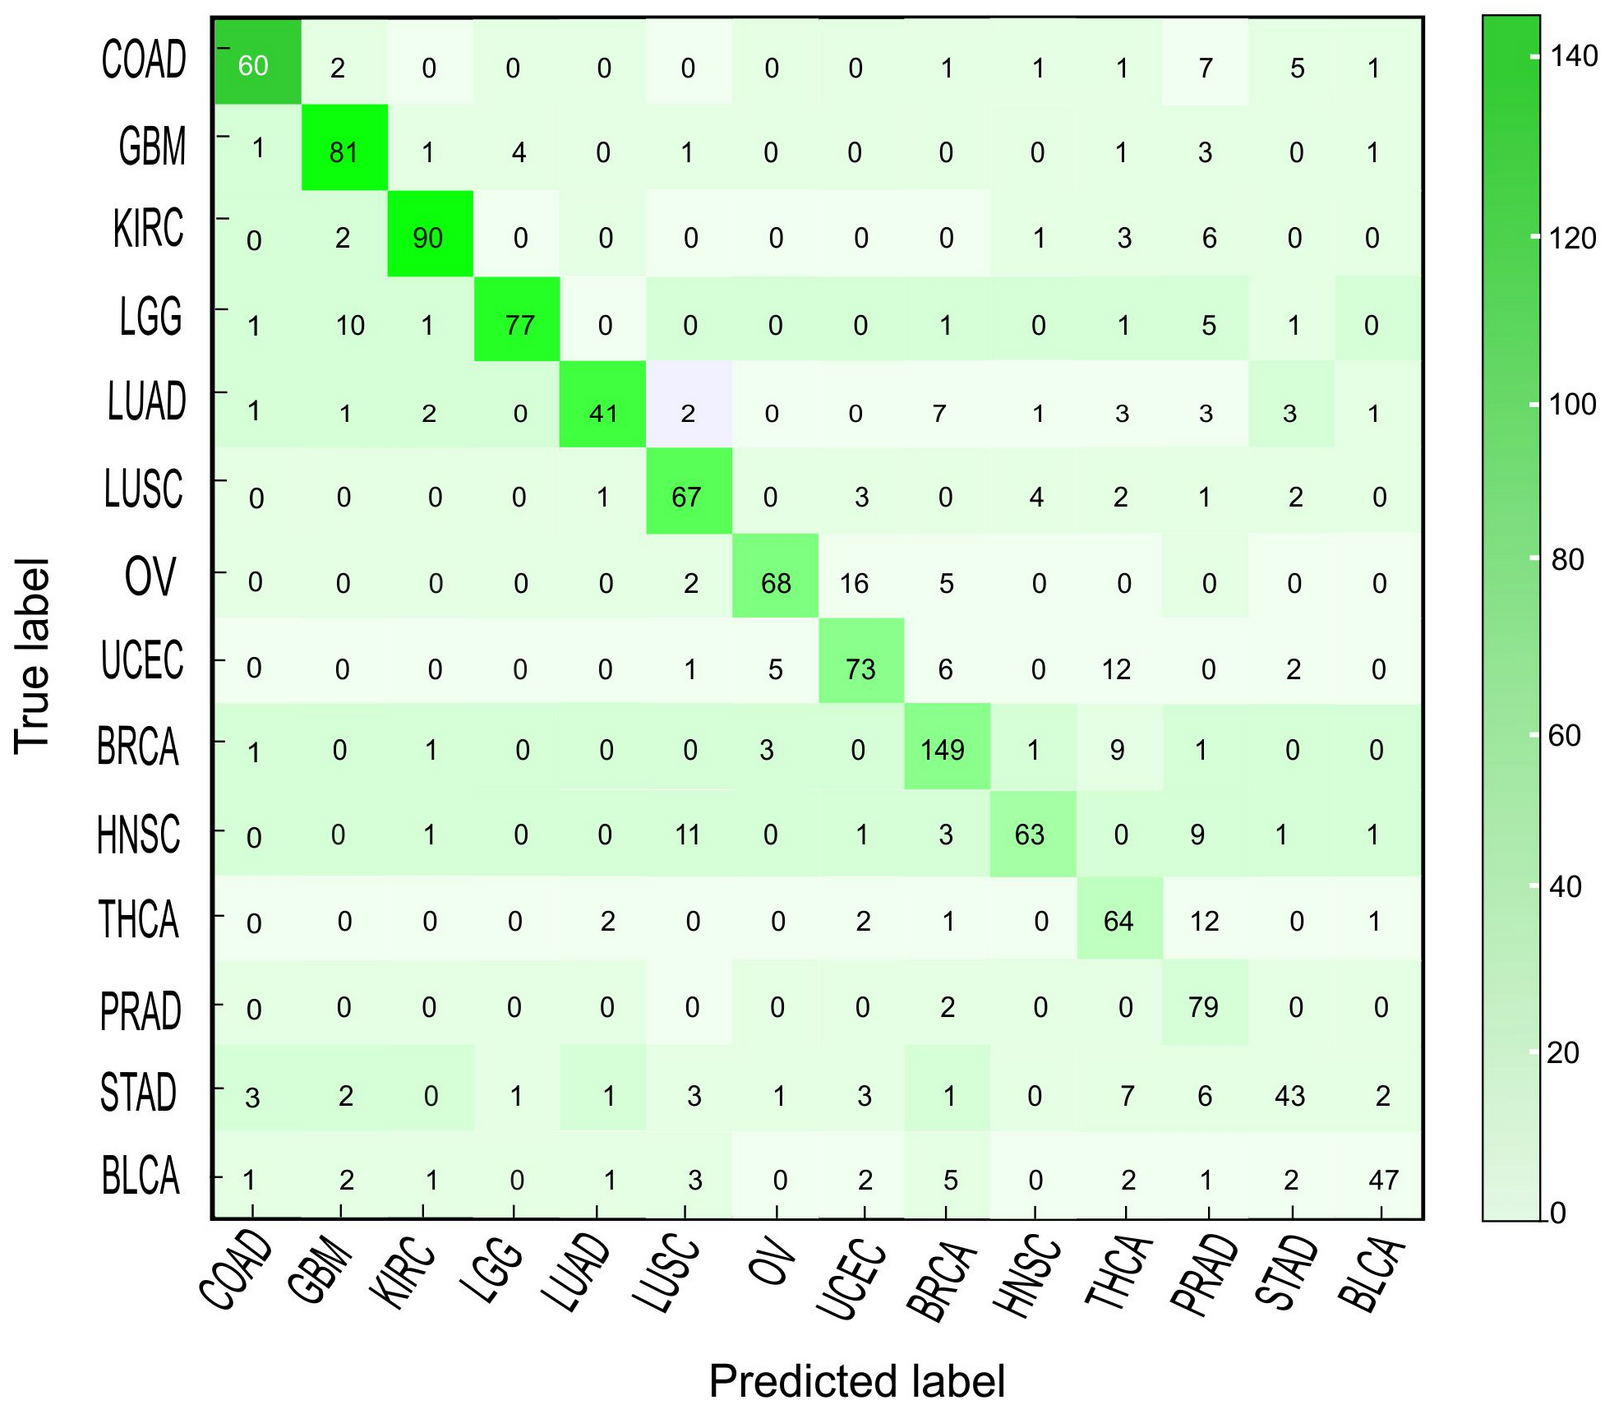
\includegraphics[scale=0.35]{images/cm2.png}
		\caption{Using oncogenes based CNVs}
        \label{fig:cm_2}
	\end{subfigure}
	\caption{Confusion matrices of the ensemble classifier} 
	\label{fig:cms}
	 \vspace{-4mm}
\end{figure}

\subsection{Performance analysis of the ensemble model}
The ensemble classifier shows about 4\% and 2\% performance boost across classes and overall in the cases of oncogenes and protein-coding gene-based experiment, respectively. The accuracy looks easy enough but makes no distinction between classes e.g., when a doctor makes a medical diagnosis that a patient has cancer, but in reality, the patient does not~(i.e., false positive). This has very different consequences than making the call that a patient does not have cancer when he actually does~(i.e., false negative). A more detailed breakdown of correct and incorrect classifications for each class using the confusion matrices is shown in \cref{fig:cms}, which correspond to ground truth labels vs. the predictions made.

\hspace*{3.5mm} There are significant accuracy improvements in case of STAD, HNSC, BLCA, THCA, UCEC, and LUSC tumor types. In case of UCEC and LUSC cancer types, not only are the accuracies increased slightly, but also the false positive rates are reduced significantly. On the contrary, using oncogenes, the classifiers were less confused among tumor types, except for the LGG, HNSC, and THCA tumor types. Despite these improvements, there is still high confusion among LUAD, HNSC, and LGG samples, which is because features from these tumor samples are highly correlated. We could not find an exact reason for such behavior. Perhaps, a more gene-specific CNV analysis is required to confirm such correlations. However, poor and imbalance training might be one of the reasons. 

\section{Discussion}\label{chapter_3:discussion}
Some previous studies~\cite{zhang2016classification,elsadek2018supervised} that focused on using CNV based cancer typing method used data from cBioPortal. They applied incremental feature selection methods before training classic ML models and managed to achieve classification accuracy of 75\% and 85\%~(by Zhang et al. and Sanaa F. et al., respectively). Since we have more samples and from different sources, a one-to-one comparison was not viable. Still, the ensemble model achieved about a classification accuracy of 80\%, which is about 6\% better than our previous approach~\cite{karim2018a2ic} w.r.t. every metric. 

\hspace*{3.5mm} However, considering an accuracy of 80\%, we cannot claim that our model’s confidence is very high. This is for several reasons, such as lack of training samples, poor training, and data sparsity. The latter reason caused each network to produce high training and validation loss of error optimization during the training phase, giving lower accuracy. Data sparsity was an issue too. In particular, on average, only 422 samples per tumor were used for the training, which is fairly low for such high-dimensional data. As a result, models are not able to identify subtle differences among tumor types. 
%We lacked enough training samples compared to the complex dataset, as deep architectures usually expect more samples to get trained well. %For the same reason, there was a lack of samples to perform model validation during 5-fold cross-validation. 
Another reason for poor training might be an imbalanced dataset. Some cancer types, such as BRCA, have 2.5 times more samples than other tumors. For example, STAD and BLCA have at least 15\% sample difference with other tumor types. These two tumors have very low classification accuracy, where about half of the samples were misclassified. Further, due to stochastic nature, ML algorithms are tend to produce different results. Besides, depending on the genome sequencing and CNV calling tools, different copy numbers might produce, with different CNV lengths and segmentation means, giving different results.

\section{Chapter Summary} \label{chapter_3:conclusion}
In this chapter, we developed a snapshot neural ensemble method for cancer-type prediction based on CNVs data using two deep architectures called Conv-LSTM and CAE. The ensemble model is based on cosine annealing techniques, which create multiple model snapshots of these networks, followed by MAE technique to combine the predictive power of these architectures.  Experiment results show that CNVs are not only useful for predicting certain types of cancer, but also show association with cancer growth. %Another type of data~(e.g., DNA methylation, gene or miRNA expression, etc.) can be used to create a multimodal network in a similar fashion of single modality-based cancer typing method. 

\hspace*{3.5mm} However, the downside of this single modality-based cancer typing method is that the findings are not validated with other annotations or scientific literature, which is why it cannot confirm if the identified genes are biologically relevant. Besides, it is not clear how the output is traced back to the inputs, nor it is clear why the outputs are transformed the way they are. Therefore, both models are `black-box'. 
On the other hand, along with accurate identification of cancer types and most relevant biomarkers are the prerequisites for an oncologist to recommend more accurate treatments and drug repositioning. The latter only can be achieved with meaningful explanations, which helps healthcare experts to make reasonable and data-driven decisions to provide personalized diagnosis~\cite{stiglic2020interpretability}.  
Further, since multiple factors are involved in accurate cancer diagnosis (e.g., estrogen receptor~(ER), progesterone receptor~(PGR), and human epidermal growth factor receptor 2~(HER2/neu) statuses for breast cancer), providing AI-based diagnoses solely based on CNVs may not be reliable.

\hspace*{3.5mm} From the carcinogenics point of view, we require multimodal features based on DNA methylation, GE, miRNA expression, and CNVs data by creating a multiplatform network to support each data type. Lastly, a DL approach using CNV data along with other types of genomics data from different cohorts such as DNA methylation, GE, and mutations will be more reliable. In the next chapter, we extend this work increasing the number of samples for training, testing, and validation, by combining samples from Pan Cancer Atlas. We will employ a multimodal neural network architecture to combine features interpret the combinations to predict the cancer subtypes. 

\chapter{Multimodal Black-box Models}
\label{chapter:multiodality}

\textit{"Learning is lifelong; we forget rules when they no longer apply or revise them when the environment changes."} - Ethem Alpaydin, Machine Learning: The New AI 

\section{Chapter Overview}
In the previous chapter, we used only CNVs, i.e., single modality to develop a decision support system~(DSS), which was technically a black-box model based on snapshot neural ensemble method in which we trained two deep architectures called \texttt{Conv-LSTM} and \texttt{CAE}. The DSS moderately performed at predicting cancer types. However, our real world experience is multimodal~\cite{mmsurvey}, e.g., while watching a movie, we not only observe the movie itself but the acting, background music, action, background scenario, and landscapes, etc. Multimodal machine learning~(ML) aims to build a ML model capable of processing and relating information from multiple modalities~\cite{mmsurvey}. Concerning our cancer CDSS, multiple factors are involved~(e.g., in cancer diagnosis, estrogen receptor~(ER), progesterone receptor~(PGR), and human epidermal growth factor receptor 2~(HER2/neu statuses for breast cancer), providing AI-based diagnoses might not be accurate solely based on CNVs. This requires using multimodal features based on DNA methylation, gene expression, miRNA expression, and CNVs data by creating a multiplatform network to support each data type, where the DSS based on CNV data along with other types of genomics data from different cohorts such as DNA methylation, gene expression, and somatic mutations will be more reliable. 

\hspace*{3.5mm} Based on this motivation, in this chapter, we extend the single modality to multimodality-based cancer typing method by employing a multimodal neural network approach to analyze genomics data from TCGA to classify breast cancer patients based on their subtypes. We hypothesize\footnote{\textbf{H1}: Multimodal genomics data and clinical outcome can be used to train a multimodal neural network architecture to provide more accurate clinical diagnostic decision.} that multimodal genomics data and clinical outcome can be used to train a multimodal neural network architecture to provide more accurate clinical diagnostic decision.
%and survival rates. 
In particular, we used DNA methylation, gene expression~(GE), and miRNA expression data by creating a multiplatform network called multimodal autoencoders~(MAE) classifier to support each data type\footnote{RQ1: How to use multimodal genomic data to accurately predict cancer
types?}. We will observe the effect of different modalities and assess the performance of our CDSS across breast cancer subtype classification. 
%Experiment results demonstrate that our approach is promising with high confidence for predicting both breast cancer subtypes and survival rates. In particular, we achieved state-of-the-art results with accuracies of $91\%$ and $86\%$, respectively for the ER and PGR-based subtype prediction and moderately low accuracy for the HER2-based subtype prediction as well as we perceived reasonably low MSE and positive coefficient of determination~($R^2$) scores in case of survival prediction. 
%Additionally, we created unimodal and multimodal features from each input type and trained decision tree~(DT), Naive Bayes~(NB), K-nearest neighbors~(KNN), logistic regression~(LR), support vector machine~(SVM), random forest~(RF), and gradient boosting trees~(GBT) as ML baseline models. We use the model averaging Ensembl of top-3 models to report the final prediction based on how the clinical DSS recommends decision. Further, we provide in details analysis of the MAE model. 

\section{Introduction}
\label{secIntroduction_Motivation}
Multimodal information fusion seeks to improve the performance of a DSS (based on an inference model) by efficiently combining useful information extracted from a set of distinctive modalities~\cite{mmdcae}. The performance of a conventional information fusion architecture is greatly affected by its ability to detect and combine useful and complementary information from heterogeneous representations stemming from a set of distinctive modalities~\cite{ito2018effects}. Multimodal fusion is the concept of integrating information from multiple modalities with the goal of predicting an outcome measure~\cite{mmsurvey,mmdcae}. Multimodal fusion provides three main benefits~\cite{mmsurvey}: i) having access to multiple modalities that observe the same phenomenon may allow for more robust predictions, making the clinical DSS more reliable, ii) having access to multiple modalities might allow us to capture complementary information, e.g., we can often integrate genomics, proteomics, bioimaging, texts, or even clinical outcomes to support each other, iii) a multimodal system can still operate when one of the modalities is missing, e.g., in case of missing bioimaging, we can still rely on genomics, proteomics, and clinical outcomes.

\hspace*{3.5mm} Concerning to the cancer DSS, accurate diagnosis and prognosis to cancer are specific to patients with particular cancer subtypes and molecular traits e.g. accurate treatments for the breast cancer patients depends on several distinct molecular subtypes such as `Luminal A', `Luminal B', `HER2-enriched', and `Triple-negative'~(TN)~\cite{sorlie,dai}, which subject to the distinction mainly determined by several factors: `Luminal A' disease generally requires only endocrine therapy, chemotherapy is considered necessary for `Luminal B', `HER2-enriched', and `Triple-negative' patients~\cite{goldhirsch}. Thus, knowing the subtypes of any breast cancer patient is essential before recommending the best possible treatment. 
TN breast cancer defined by ER, PGR, and HER2, represents a subset of breast cancer with different biologic behavior. ER, PGR, and HER2 statuses are mainly involved in determining breast cancer subtypes. %and survival rates. 
Further, those patients can be categorized into different classes. For example, ER `POSITIVE', `NEGATIVE', or `INDETERMINATE'. The ER-negative tumors are associated with a worse clinical outcome compared to ER-positive disease. An accurate estimate of the hazard ratio between ER-negative tumors and ER-positive tumors remains difficult and prone to higher misclassification~\cite{karimACCA2019}. 
%As cancer is a disease that was caused by genetic mutations, more extensive knowledge of each mutation might result in the further distinction of breast cancer subtypes.
%The survival rate, on the other hand, suggests the chance of survival based on patients clinical and pathology information, which are further dependent on the in-depth analysis of these status biomarkers. %An analysis of genetic mutations directly on the survival rate data might tell the whole picture of why some genetic mutations might cause the worst cancer than other mutations.

\hspace*{3.5mm} In order to develop a more robust and efficient DSS, it needs to be able to interpret such multimodal perspectives together~\cite{mmsurvey}. However, multiple modes of information are gathered to create knowledge in a way humans can understand~\cite{mmdcae}. However, each type of data has different intrinsic statistical features that cannot be compared in a trivial way, nor they can be combined. In this chapter, we develop a clinical DSS using DNA methylation, GE, and miRNA expression data in a single analysis by creating an MAE to handle the shared representation of the multiplatform data to support each other. We hypothesize\footnote{    \textbf{$H_2$}: neural representation learning can be more effective for learning high-level abstract features against data sparsity.} that neural representation learning can be more effective for learning high-level abstract and multimodal features against data sparsity. 
The rest of the chapter is structured as follows: \cref{chapter_4:rw} covers related works concerning cancer diagnosis based on multimodality data and summarize their potential limitations. \Cref{chapter_4:mm} describes the overall approach, including the detail of the data collection and feature engineering before the network construction and training. \Cref{chapter_4:results} demonstrates the experiment results. \Cref{chapter_4:discussion}, discusses key findings of the study. \Cref{chapter_4:conclusion} provides some explanations of the importance and relevance of the study reported, highlights the limitations and discuss some future works before concluding the chapter. 

\section{Related Work}\label{chapter_4:rw}
The multilayer nature of DNN's each successive layer is hypothesized to represent the data in a more abstract way~\cite{mmsurvey}. Hence it is common to use the final or penultimate neural layers as a form of data representation~\cite{mmsurvey,serban2016multi}. To construct a multimodal representation using neural networks each modality starts with several individual neural layers followed by a hidden layer that projects the modalities into a joint space~\cite{serban2016multi}. The joint multimodal representation is then be passed through multiple hidden layers itself or used directly for prediction. Such models can be trained end-to-end-learning both to represent the data and to perform a particular task, e.g., classification. This results in a close relationship between multimodal representation learning and multimodal fusion when using DNN~\cite{wang2018associativemulti}.

\hspace*{3.5mm} The model proposed by Ngiam et al.~\cite{NgiamKKNLN11} extended the idea of using autoencoders to the multimodal domain. They used stacked denoising autoencoders to represent each modality individually and then fused them into a multimodal representation using another autoencoder layer~\cite{mmsurvey,serban2016multi}. It is also common to fine-tune the resulting representation on a supervised learning tasks such as regression or classification. The major advantage of DNN-based joint representations comes from their often superior performance and the ability to pre-train the representations in an unsupervised manner. The performance gain is, however, dependent on the amount of data available for training. One of the disadvantages comes from the model not being able to handle missing data, which is mainly due to the reconstruction losses during the pre-training goes unbound. Usually, a DNN require a lot of labeled training data. Therefore, it is common to pre-train such representations using an autoencoder on unsupervised data~\cite{mmsurvey}. 

\hspace*{3.5mm} Even a few years ago, most popular approaches for graphical-model based representation are deep Boltzmann machines~(DBM), that stack restricted Boltzmann machines~(RBM) as building blocks. Similar to DNNs, each successive layer of a DBM is expected to represent the data at a higher level of abstraction. The appeal of DBMs comes from the fact that they do not need supervised data for training. As they are graphical models the representation of data is probabilistic, however it is possible to convert them to a deterministic DNNs, which, however, loses the generative aspect of the model. Although, approaches using both unimodal~\cite{abdel2016breast} and multimodal DBN~\cite{liang} show accuracy at different prediction tasks, one of the potential limitations using DBN-based approaches is that the limited capability at feature learning during pretraining~\cite{serban2016multi}, although it gets a decent set of feature representations for the inputs. Furthermore, DBN is incapable of learning quality features from very high dimensional datasets. Besides, pretraining losses often get out of bound, which results in overfitting issue. 

\hspace*{3.5mm} To overcome these limitations, majority of the multimodal methods focused on representation fusions~\cite{ito2018effects}, either by combining representations before the classification called feature level fusion or by combining the results of classifications performed in single-mode representations in another analysis  called `decision level fusion'~\cite{atrey2010multimodal}. In particular, researches have proposed multimodal autoencoder~(MAE)-based approaches~\cite{liu2016multimodal,serban2016multi,wang2018associativemulti}, which is a flexible, simple prior distribution which can be learned efficiently and potentially capture from extensive features of a target distribution. Consequently, MAE has shown tremendous success in natural language understanding tasks like document modeling and dialogue modeling~\cite{serban2016multi}, in computer vision like emotion recognition~\cite{liu2016multimodal}, and multimodal word representation~\cite{wang2018associativemulti}. 

\hspace*{3.5mm} An alternative to a joint multimodal representation is a coordinated representation, where instead of projecting the modalities together into a joint space, separate representations for each modality are learned but coordinated them through a constraint. Inspired by these successes, we construct a MAE network by extending the multimodal system presented in~\cite{wang2018associativemulti} by adding the capability of handling multiple modalities across four different types of genomics data. Then we added a fully connected layer for the supervised learning task, i.e. breast cancer subtypes predictions. However, our datasets are very rich, covering all the modalities for $93\%$ of patients. In our approach, we apply multimodal fusion approach by discarding the small part of patient data that don't have all modalities in our MAE network. Although, there a few recent multimodal approaches for more optimized representation learning, in this chapter we will observe the performance of vanilla autoencoder-based MAE architecture. 

\section{Methods}\label{chapter_4:mm}
In this section, we discuss our approach in detail, including data collection, preprocessing, network construction, and training. 

\subsection{Problem statement}
%Although breast cancer patients now have one of the best survival rates among other cancer types, improved studies on breast cancer are still a non-trivial research problem. 
%We focus here on the difficult problem of finding sub types of breast cancers. 
Since we conceive finding the importance of extensive knowledge about genetic mutations in breast cancer aiming to help in discovering more suitable treatments for each breast cancer subtypes, we show which genetic mutations are responsible for which breast cancer subtypes~(with feature selection). % or have direct correlations on the survival rates.  %, which is because certain genetic mutations might have a direct correlation on survival rates. %To summarize, the following tasks will be completed:
For the breast cancer subtypes prediction, we used genomics data accompanied by ER, PGR, and HER2/neu status that are present inside breast cancer patients for each patient either separately or in a multimodal way. 
%In the context of survival rate prediction, our network should tell us the chance of survival for each cancer patient based on individual patient's clinical and pathology information. The survival rate ranges between [0-1], with 1 being the highest chance of survival.
%Since data is essential for training the MAE model, 
We provide the details of the data collection, processing, and feature selection in details. 

\begin{sidewaysfigure*}
	\centering
	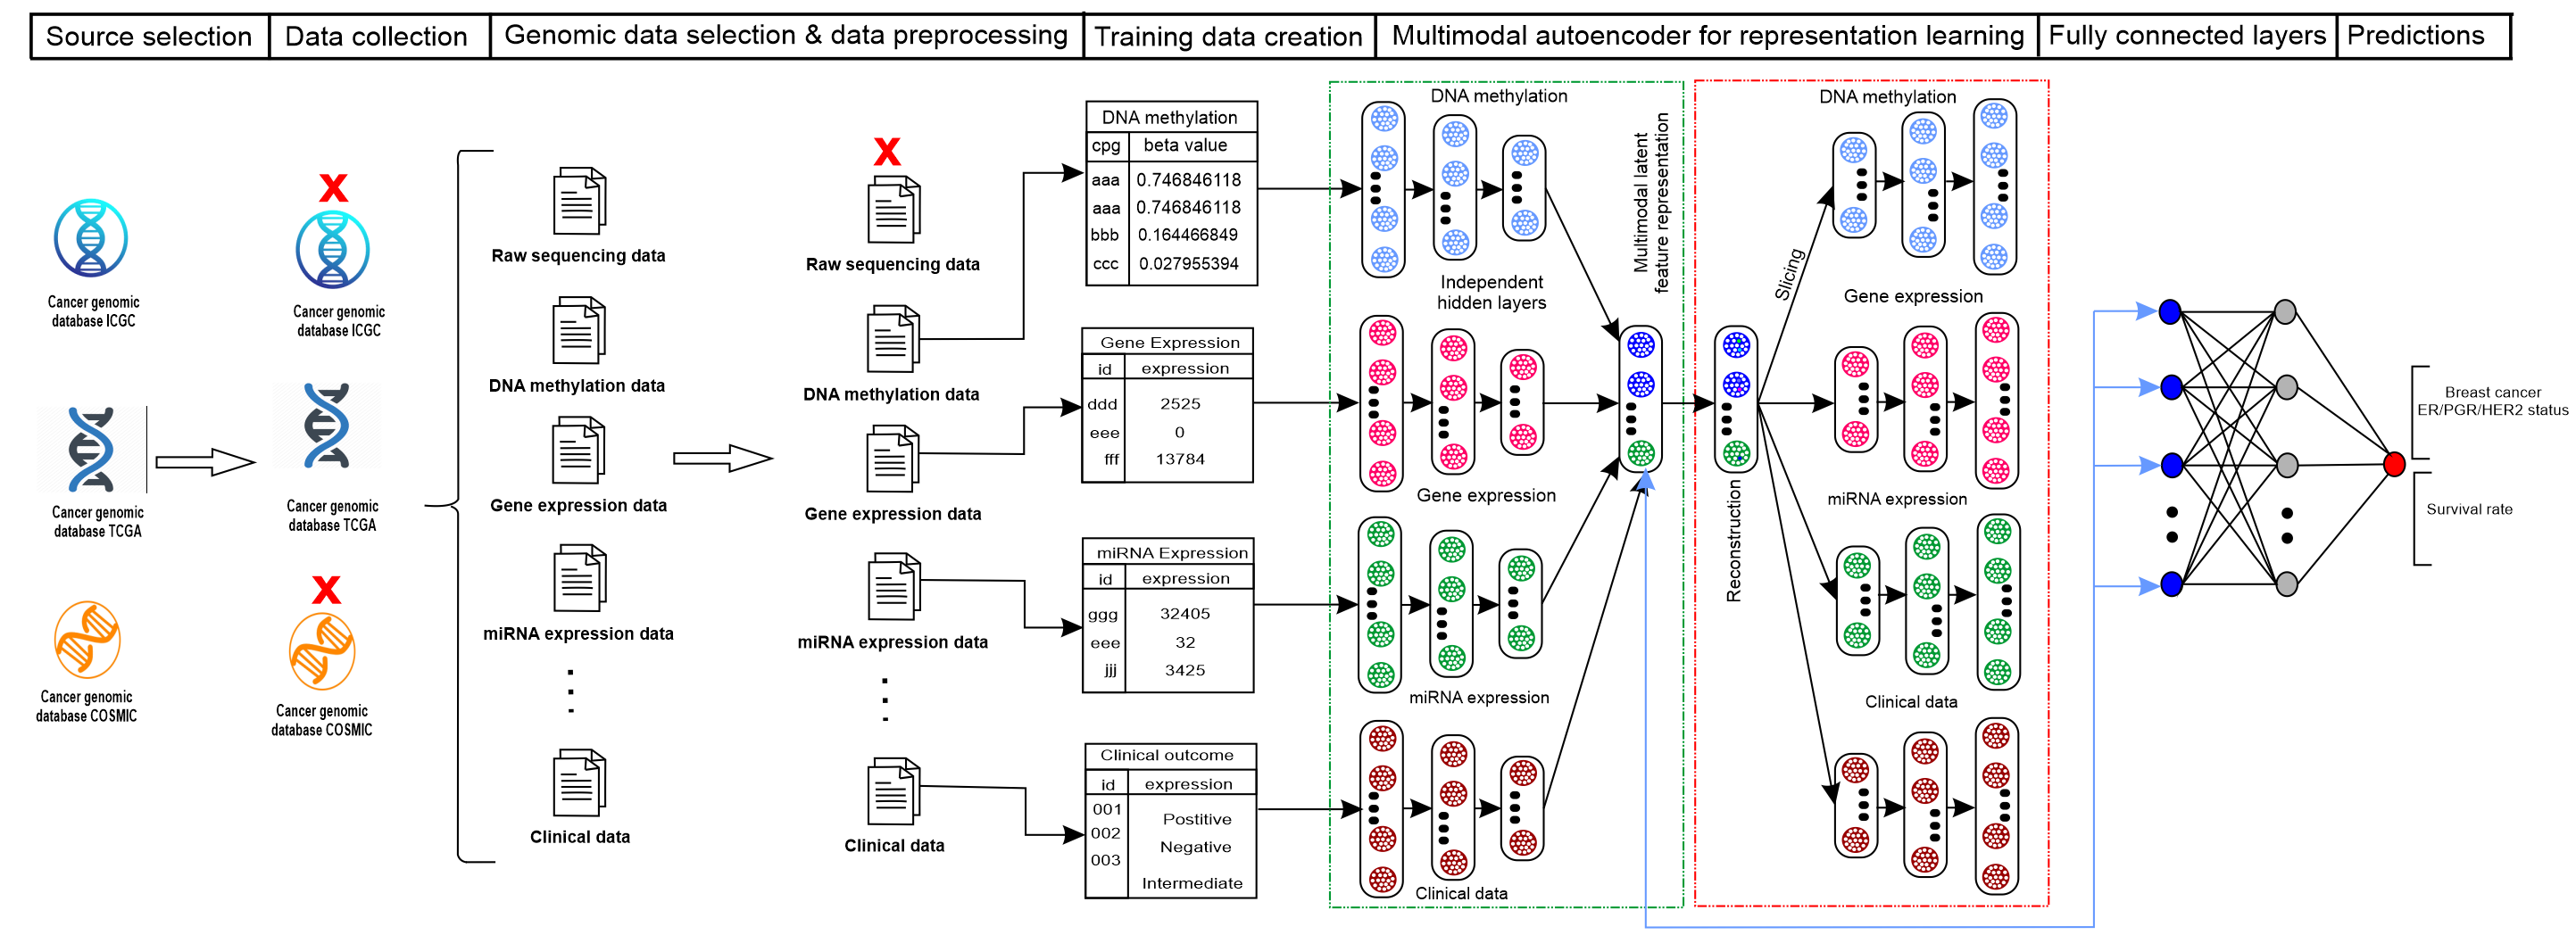
\includegraphics[width=\textwidth]{images/mae_v2.png}
	\caption{Workflow of the proposed approach in which same input types with different features for subtypes %and survivals 
	are used~\cite{karimACCESS2019}.}
	\label{fig:wf_mae}
\end{sidewaysfigure*}

\subsection{Datasets and feature selection}
\label{dc}
Although genomics data covers all data related to DNA on living organisms, we use transcriptomics data, including RNA and miRNA. These genomics data are usually accompanied by clinical outcomes, which comprise of general clinical information as well as cancer status (e.g., cancer location, cancer stage). These data are also very high-dimensional, e.g., GE data for each patient, which is structured based on gene id reaches around 60,000 types, meaning a predictor based on GE comes with 60,000 different features. Several databases of genomics data exist including TCGA~\cite{tcga}, ICGC~\cite{icgc}, and COSMIC~\cite{forbes}. However, based on public availability and amount of data consideration, e.g., the number of patients data and clinical outcomes, we considered the breast invasive carcinoma~(BRCA) branch of TCGA as the main source of data\footnote{TCGA has 39 projects for 39 different cancer types~(v89)}. After selecting data sources, we start collecting both clinical data and biospecimens through the Genomics Data Commons~(GDC) data portal\footnote{\url{https://portal.gdc.cancer.gov/}}. 

\hspace*{3.5mm} To provide more reliable cancer identification 
%and the decision about survival
, several modalities consisting of masked somatic mutations, copy number segment~(CNS) and mask CNS, DNA methylation, GE, miRNA expression along with clinical outcomes were used, instead of a single modality. Besides, some preprocessed data were reused\footnote{Based on a Master thesis I co-supervised with Dr. Oya Beyan: "Analysis of Breast Cancer Genomic Data with Multimodal Deep Belief Network", by Galih Wicaksono, Software Systems Engineering, RWTH Aachen University, 2018.}. Some of the data comes in different formats, e.g., $70\%$ of the DNA methylation data of breast cancer patient came from a different platform than the remaining $30\%$, having two structures. 

\begin{table}[h]
    \scriptsize
    \caption{Statistics of the data used for breast cancer sub-typing~\cite{karimACCESS2019}}
    	\vspace{-2mm}
    \label{tab:all_data_brca}
    \centering
    \begin{tabular}{l|l|l|l} 

        \hline
        \textbf{Tasks}   & \textbf{Input modality} & \textbf{\#Sample } & \textbf{\#Features}  \\ 
        \hline
             & DNA methylation  & 1,046  & 25,978  \\ 
        \cline{2-4}
               & Gene expression   & 1,042 & 60,483      \\ 
        \cline{2-4}
        ER status classification       & miRNA expression                           & 1,029                & 1,881       \\ 
        \cline{2-4}
                                       & Gene + miRNA expression                   & 1,024                & 62,364      \\ 
        \cline{2-4}
                                       & Gene + miRNA expression + DNA methylation & 1,022                & 88,342      \\ 
        \hline
                                       & DNA methylation                           & 1,045                & 25,978      \\ 
        \cline{2-4}
                                       & Gene expression                           & 1,041                & 60,483      \\ 
        \cline{2-4}
        PGR status classification      & miRNA expression                           & 1,028                & 1,881       \\ 
        \cline{2-4}
                                       & Gene + miRNA expression                   & 1,023                & 62,364      \\ 
        \cline{2-4}
                                       & Gene + miRNA expression + DNA methylation & 1,021                & 88,342      \\ 
        \hline
                                       & DNA methylation                           & 917                  & 25,978      \\ 
        \cline{2-4}
                                       & Gene expression                           & 913                  & 60,483      \\ 
        \cline{2-4}
        HER2/neu status classification & miRNA expression                           & 902                  & 1,881       \\ 
        \cline{2-4}
                                       & Gene + miRNA expression                   & 897                  & 62,364      \\ 
        \cline{2-4}
                                       & Gene + miRNA expression + DNA methylation & 895                  & 88,342      \\ 
        \hline
        \iffalse
                                       & DNA methylation                           & 1,082                & 25,978      \\ 
        \cline{2-4}
                                       & Gene expression                           & 1,077                & 60,483      \\ 
        \cline{2-4}
        
        Survival prediction            & miRNA expression                           & 1,064                & 1,881       \\ 
        \cline{2-4}
                                       & Gene + miRNA expression                   & 1,058                & 62,364      \\ 
        \cline{2-4}
                                       & Gene + miRNA expression + DNA methylation & 1,056                & 88,342      \\ 
        \hline
        \multicolumn{1}{l}{}           & \multicolumn{1}{l}{}                      & \multicolumn{1}{l}{} &  
        \fi 
    \end{tabular}
    	\vspace{-4mm}
\end{table}

\hspace*{3.5mm} However, in our case, several factors refrained us from using each type of data, e.g. masked somatic mutation data are the base pair~(BP) position in a chromosome but 
%The total number of base pairs in a single human cell 3 billion and 
not all the mutations are significant. Even if we use them, the generated dataset will be very sparse. %giving too many zero entries. 
The CNS and masked CNS data were not used because of extremely high dimension and complex structure of the data, and there was no fixed dimension for each data per patient. Since BP's start refers observed, CNS data and stop positions in a chromosome, which will always vary at a BP resolution.
%We do not use here copy number and DNA variation gave the extremely high dimension and complex structure of the data, i.e., variant position, will always vary at a base pair resolution.
With these considerations, DNA methylation, GE, and miRNA expression data along with clinical data containing pathology response data are used. 
%and the survival rate data are used.
Since the GE quantification data covers the amount of RNA synthesized by each gene on a single time, we treat each data per row and consider if the gene's Ensembl Id belongs to the Ensembl Id Release 89. The miRNA expression quantification and GE quantification data from TCGA were already in the desired format, so no preprocessing was required. 
%From the masked somatic data, gene data containing both the Ensembl ID and Hugo gene symbol considered only. Since both CNS and masked CNS data cover entire gene mutation cases on base-pair sequences instead of a single BP case, which was covered in masked somatic data, we find corresponding Ensembl gene ID from the chromosome position and extract the data using Ensembl API~\cite{yates}. 

\hspace*{3.5mm} However, processing DNA methylation data was a complex task as some patients were measured with the HumanMethylation27 platform. The remaining patients were measured with HumanMethylation450 arrays, which measures 450.000 methylation sites, being only 26K DNA methylation sites were considered in common to both platforms. We combined these data in seven modalities:~DNA methylation, GE, miRNA expression, GE+miRNA expression, DNA methylation+GE+miRNA expression, GE+DNA methylation, and miRNA expression+DNA methylation within the data\footnote{Last two modalities were used for the training and evaluation but not reported due to low accuracies.}. \Cref{tab:all_data_brca} shows the statistics of the preprocessed data for each modality. We find corresponding Ensembl gene IDs from the chromosome position based on GDC API. The samples having the latest gene Ensembl IDs from Release 89 are only considered valid. Clinical data covers clinical outcomes of cancer patient treated as general, pathology, treatments, and surgery. We categorized each patient data into different groups, but only the pathology response 
%and the survival data 
from the whole clinical outcomes are used. 

%\subsection{Selection of neural networks}
%We restrict our selection on DNN architecture based on the types of data: since we don't have enough labeled data, using CNN was not a viable option at first place because an end-to-end CNN requires huge data to get trained well. Secondly, since the data at our hand is not in sequence format (e.g., raw DNA sequence or protein sequence), we decided not to use RNN types networks. 
%Thirdly, the multimodality nature of the input data further motivated us developing a deep multimodal architecture called Multimodal Autoencoders~(MAE).% input which includes different type of data (e.g., audio and video), which was first proposed by Ngiam et al\cite{NgiamKKNLN11}. 

\subsection{Network construction and training}
The multimodality nature of the input data further motivated us developing the MAE. Although a single and simple AE discussed in \cref{preli:AEs} can reconstruct an output similar to the original input, it cannot handle multimodality~(i.e., different types of information). Nevertheless, traditional supervised learning is only able to learn from the intersection of samples, which are both clean and labeled. In contrast, the weights of the MAE encoder learn from both clean, unsupervised data with no labels, and noisy supervised data with missing modalities, leveraging as much of the available data as possible. Architecturally, MAE is similar to a three-stage AE: the first stage represents a particular modality for each type of data, and the second stage represents the cross-modality. The AE is used to find a low-dimensional representation of multimodal data, taking advantage of the information that one modality provides about another. We illustrate the construction of an MAE as a quad-modal AE for this problem. Where DNA methylation, GE, miRNA expression, and clinical outcomes form four different modalities. 

\hspace*{3.5mm} The individual modality AE is not only a one-layer AE, but a multilayer and gradually shrinking AE with the possibilities of a different number of layers for each modality, which is due to the difference in dimension between modalities are pretty large, e.g. GE data consists of around 60,000 features, while miRNA data only consists of around 1,800. By default, the AE network fusing multiple modalities consists of a variable number of ReLU layers, which are densely connected. The cross-modality AE is also a multilayer gradually shrinking AE with different size of output layer for each prediction. However, the number of layers and number of units per layer of the encoder and decoder networks are symmetric. The third stage is the supervised MAE in which the decoder part is removed, and only the encoder part is utilized by adding a fully connected layer. % for the classification. %and regression operations. 
First, data $X_{i,j} \in \mathbb{R}^{D}$, for each modality $i \in \mathbb{N}$\footnote{N represents the dimensionality of the $i^{th}$ input modality} is fed into the encoder $f_{\theta_{i}}$ in order to generate a modality specific latent representation $h_{i, j}$ as follows~\cite{mmdcae}: 

\vspace{-4mm}
\begin{align}
    h_{i, j}=f_{\theta_{i}}\left({X}_{i, j}\right)
\end{align}

where $f_\theta$ signifies trainable parameters of the encoder specific to the $i^{th}$ modality. Subsequently, the latent representation is then fed into the decoder module to reconstruct ${X}_{i, j}^{\prime}$ similar to the original input. The parameters of the modality specific AE are then then trained to minimize the RL1 between the decoder’s output and the input signal, where the RL1 is similar \cref{eq:Loss1}. The latent representations of all modalities are further concatenated into a single representation $h_{i,j} \in \mathbb{R}^{D}$. 

\hspace*{3.5mm} However, in order to create such a shared representation, it is required that all latent representations have the same dimensionality such that $\forall i \in\{0,1, \ldots, n\}, d_{i}=$ $\eta \in \mathbb{N}$~\cite{mmdcae}. On the other hand, the architecture depicted in \cref{fig:slr_1} generates the shared representation for all input modalities, instead of one latent representation for each input modality. However, for the simplicity, in this chapter, we use the shared representation for all input modalities. In either approach, the resulting concatenated generates a single vector $u=\left[u_{0}, u_{1}, \ldots, u_{n}\right] \in[-1,1]^{(n+1) \eta}$, where the weights of the corresponding components are generated using the softmax layer as follows~\cite{mmdcae}:

\vspace{-6mm}
\begin{align}
    \omega=\operatorname{softmax}\left(W_{\omega} u+b_{\omega}\right),
\end{align}

where $\omega=\left[\omega_{0}, \omega_{1}, \ldots, \omega_{n}\right] \in[0,1]^{(n+1) \eta}$ $\left(\forall i, \omega_{i} \in[0,1]^{\eta}\right)$, and  $W_{\omega} \in$
$\mathbb{R}^{(n+1) \eta \times(n+1) \eta}$ and $b_{\omega} \in \mathbb{R}^{(n+1) \eta}$ is the trainable parameters ~\cite{mmdcae}. The final latent representation is generated through a weighted sum of all the modalities specific latent representation $\left(h_{i,j}\right)$ based on the computed weights $\left(\omega_{i}\right)$ as follows~\cite{mmdcae}: 

\vspace{-4mm}
\begin{align}
   h_{i,j}=\sum_{i=1}^{n}\left(h_{i} \odot \omega_{i}\right),
\end{align}

where $\odot$ denotes the element-wise product and $h \in$ $\mathbb{R}^{\eta}$ is the final representation~~\cite{mmdcae}, which is subsequently fed to the classifier for the classification. In our approach, as shown in ~\cref{fig:wf_mae}, our model first transforms input DNA methylation vector $x_m$, GE vector $x_e$, miRNA expression vector $x_r$, and clinical data vector $x_c$ to hidden representations~\cite{wang2018associativemulti}.

\vspace{-4mm}
\begin{align}
    \begin{array}{l}
        {h_{m}=g\left(W_{m} x_{t}+b_{m}\right)} \\
        {h_{e}=g\left(W_{e} x_{v}+b_{e}\right)} \\
        {h_{r}=g\left(W_{r} x_{a}+b_{r}\right)} \\
        {h_{c}=g\left(W_{c} x_{t}+b_{c}\right)}
    \end{array}
    \label{eq:m1}
\end{align}  

Then the hidden representations are concatenated together and mapped to a common space~\cite{liu2016multimodal}:

\vspace{-4mm}
\begin{equation}
    h_{mae}=g\left(W_{mme}\left[h_{m} ; h_{e} ; h_{r} ; h_{c}\right]+b_{mme}\right)
\end{equation}

The model is trained to reconstruct the hidden representations of the three modalities $h_{mae}$:

\vspace{-4mm}
\begin{equation}
    \left[\hat{h}_{m} ; \hat{h}_{e} ; \hat{h}_{r} ; \hat{h}_{c} \right]=g\left(W_{mae}^{\prime} h_{mae}+b_{\hat{mae}}\right)
\end{equation}

To reconstruct the original representation of different modalities i.e., DNA methylation, gene expression, miRNA expression data, and clinical outputs~\cite{wang2018associativemulti}: 

\vspace{-4mm}
\begin{align}
    \begin{aligned}
        \hat{x}_{m} &=g\left(W_{m}^{\prime} \hat{h}_{m}+b_{\hat{m}}\right) \\
        \hat{x}_{e} &=g\left(W_{e}^{\prime} \hat{h}_{e}+b_{\hat{e}}\right) \\
        \hat{x}_{r} &=g\left(W_{r}^{\prime} \hat{h}_{r}+b_{\hat{r}}\right) \\
        \hat{x}_{c} &=g\left(W_{c}^{\prime} \hat{h}_{c}+b_{\hat{c}}\right)
        \end{aligned}
\end{align}

where $\hat{x}_{m}$, $\hat{x}_{e}$,  $\hat{x}_{r}$, $\hat{x}_{c}$ are the reconstruction of input vectors $x_{m}$, $x_{e}$, $x_{r}$, $x_{c}$, where by randomly blocking out different modalities from the training data and learning to reconstruct them, the MAE attempts to reconstruct the original data $\hat{h}_{m}$, $\hat{h}_{e}$, $\hat{h}_{r}$, and $\hat{h}_{c}$ are the reconstruction of hidden representations ${h}_{m}$, ${h}_{e}$, ${h}_{r}$, and ${h}_{c}$~\cite{wang2018associativemulti}. The last element of the hidden dimension is the dimensionality of the latent space representation and the decoder module has similar gradual increasing architecture. The learning parameters $   \theta=\left\{W_{m},W_{e},W_{r},W_{c},W_{m}^{\prime},W_{e}^{\prime},W_{r}^{\prime},W_{c}^{\prime},W_{mae},W_{mae}^{\prime}\right\}$ are weight matrices, $\left\{b_{m}, b_{e}, b_{r}, b_{c}, b_{\hat{m}}, b_{\hat{e}}, b_{\hat{r}}, b_{\hat{c}}, b_{mae}, b_{\hat{mae}}\right\}$ are bias vectors, $[.;.]$ denotes the vector concatenation, and $g$ denotes the $ReLU(.)$ activation function~\cite{wang2018associativemulti}. 

\hspace*{3.5mm} Similar to literature~\cite{wang2018associativemulti,serban2016multi}, noise distributions are taken into account employing Bregman divergences~(BD), which corresponds to particular exponential families such as Gaussian, Poisson or gamma distributions. Each modality can have its own BD as loss function, thereby assuming a specific noise of output distribution. The unsupervised pre-training is performed greedily on each layer of the MAE, which corresponds to the nature of AE. The three-stage MAE creates hierarchical hidden units, which have strong connections between nodes not only for individual modality but also across the modalities. 
%For example, the survival rate prediction will only consist of one neuron in the output layer, while 
The breast cancer subtype classification and the treatment response classification both will consist of more than one neuron in the output layer. 
%We generalize the MAE for both breast cancer subtype classification and survival rate prediction. 

\hspace*{3.5mm} The datasets are formed from any combinations of three genomics data, including DNA methylation, GE, and miRNA expression. Since the breast cancer subtype classification consists of three sub-tasks based on ER, PGR, and HER2/neu status, each of these will correspond to their neural networks. First, we focus on the ER status classification by determining the existence of ER protein inside breast cancer patient. The status can be `POSITIVE', `NEGATIVE', or `INDETERMINATE'\footnote{Patients can't be grouped as positive, negative, or equivocal}, which means our network predicts one of three classes. The input to the network can be a single or multimodality in combination with DNA methylation, GE, or miRNA expression data as shown in~\cref{tab:all_data_brca}. The second type of breast classification is the PGR status classification, which determines the existence of PGR protein inside breast cancer patient. Just as ER status, PGR status is also classified into `POSITIVE', `NEGATIVE', or `INDETERMINATE', which means the model will predict one of three classes. Nevertheless, we use single type input with a regular AE and multiple types of input with an MAE. 

\hspace*{3.5mm} For each model, we have specific input modality as outlined in~\cref{tab:all_data_brca}. The third type of breast subtype classification is based on the HER2/neu, which determines the existence of HER2 in the breast cancer patient. Unlike ER and PGR status, HER2/neu status is the most important predictive and prognostic biomarker in breast cancer, which is classified into four types: `POSITIVE', `NEGATIVE', `INDETERMINATE', and `EQUIVOCAL'\footnote{Assessments without information on how to treat a patient}. Similar to ER and PGR subtyping, both unimodal inputs with a regular AE and multimodal input with MAE are used for the HER2/neu based classification as shown in~\cref{tab:all_data_brca}. 
%The survival rate ranges between 0-1, where 1 indicates the highest chance of survival. Due to the continuous nature of the output, we model this as the regression task, which we implement using both single type input with a regular AE and multiple types of input with an MAE. 
We perform unsupervised pre-training for the whole layer of MAE, which is followed by a supervised fine-tuning for either subtype classification or survival rate prediction. During the pretraining phase, we utilized the whole datasets for the training with 10\% for the validation. Training a single-layer autoencoder corresponds to optimizing the learning parameters to minimize the overall loss between inputs and their reconstructions, which can be defined as follows:

\vspace{-2mm}
\begin{equation}
   L_{r} = \min _{\theta} \sum_{i=1}^{n} \left\|x_{t}^{i}-\hat{x}_{t}^{i}\right\|^{2}+\left\|x_{v}^{i}-\hat{x}_{v}^{i}\right\|^{2}+\left\|x_{a}^{i}-\hat{x}_{a}^{i}\right\|^{2}
   \label{eq:recons_loss}
\end{equation}

where $i$ denotes the $i^{th}$ feature. The latent representations of all the input modalities are subsequently concatenated into a single representation $h_{i,j} \in \mathbb{R}^{D}$ and used into the feed-forward neural network for the classification, which is trained to optimize the categorical cross-entropy~(CE) loss~\cref{eq:cross_entropy_loss} of the predicted cancer subtype $Y \prime$ vs. actual subtype $Y$. 

\vspace{-2mm}
\begin{equation} 
    L_{c}=-\sum_{k=1}^{D}\left[Y_{k} \log Y_{k}^{\prime}+\left(1-Y_{k}\right) \log \left(1-Y_{k}^{\prime}\right)\right]
    \label{eq:cross_entropy_loss}
\end{equation} 

\hspace*{3.5mm} The softmax activation function is used in the output layer for the probability distribution over the classes for breast cancer subtype prediction. 
%On the other hand, for the survival prediction, we optimize the MSE between the predicted survival rate vs actual survival rates. 
Eventually, the parameters of the entire MAE  architecture are optimized by minimizing the following objective function~\cite{mmdcae}:

\vspace{-4mm}
\begin{align}
    {L}=\sum_{i=0}^{n} \alpha_{r} {L}_{r}+\alpha_{c} {L}_{c}
    \label{eq:sum}
\end{align}

\hspace*{3.5mm} where the parameters $\alpha_{r}$ and $\alpha_{c}$ are regularization weights assigned to each error function~\cite{mmdcae}. Before the training, the MAE network parameters were initialized with Xavier initialization~\cite{xavier} and trained using first-order gradient-based optimization techniques AdaGrad. The training process is performed through a total of 100 epochs with the batch size set to $128$. The activity regularization term of \cref{eq:recons_loss} is set between $\lambda=[0.001, 0.005]$, while the regularization weights of the loss functions in \cref{eq:sum} are set as  $\alpha_{0}=\alpha_{1}=\alpha_{2}=0.1$, and $\alpha_{c}$=0.25. The weight of the classifier's loss function is set greater than the others to focus more on the classification performance of the whole architecture. Further, we observe the performance by adding the Gaussian noise layers followed by the dense layer to improve model generalization and reduce overfitting, where the Gaussian noise parameters are empirically set to a standard deviation of 0.1 and a mean of 0. 

\section{Experiments}\label{chapter_4:results}
%All program were implemented in Python using scikit-learn and Keras with TensorFlow backend\footnote{\url{https://github.com/rezacsedu/MultimodalAE-BreastCancer}}. The network training was done on an Nvidia GTX 1050 GPU with CUDA and cuDNN enabled to make the overall pipeline faster. 
%\subsection{Experiment setup}
In this section, we analyse the results both quantitative and qualitatively. 
The full training set is used for pretraining the MAE in which 10\% data is used for the validation, followed by supervised fine-tuning with 70\% of the training data. The trained model is then evaluated on the 20\% held-out test set. Results based on best hyperparameters produced through random search and 5-fold cross-validation tests empirically are reported in which macro-averaged precision, recall, F1, and Matthias correlation coefficient~(MCC) score, confusion matrices, and receiver operating characteristic~(ROC) curves are interpreted.
%; while the standard mean squared error~($MSE$) and coefficient of determination~($R^2$) are computed to assess the performance of the survival rate prediction.% of the clinical DSS. %Since this is one of the very first works on multimodality learning, comparing our approach with baseline models was not a viable option. 

\begin{sidewaysfigure*}[htp!]
	\centering
	\begin{subfigure}{.49\linewidth}
		\centering
		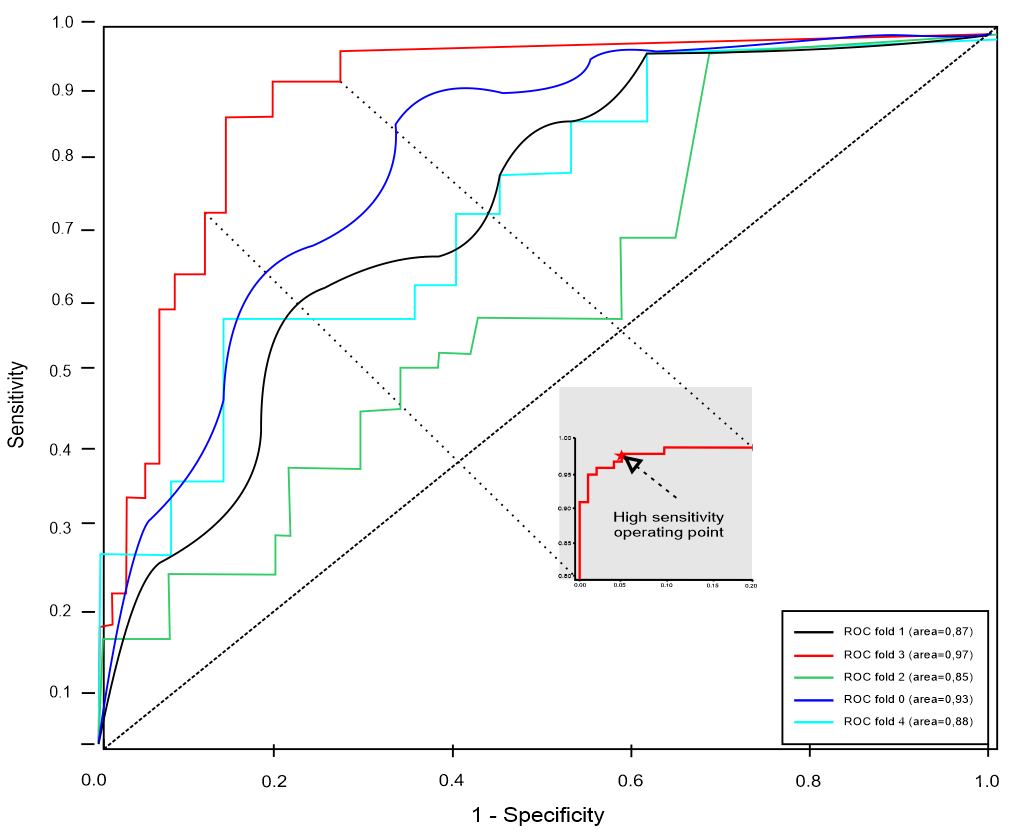
\includegraphics[width=0.9\linewidth]{images/roc_er.png}
		\caption{ER status classification}
        \label{fig:er_roc}
	\end{subfigure}
	\begin{subfigure}{.49\linewidth}
		\centering
		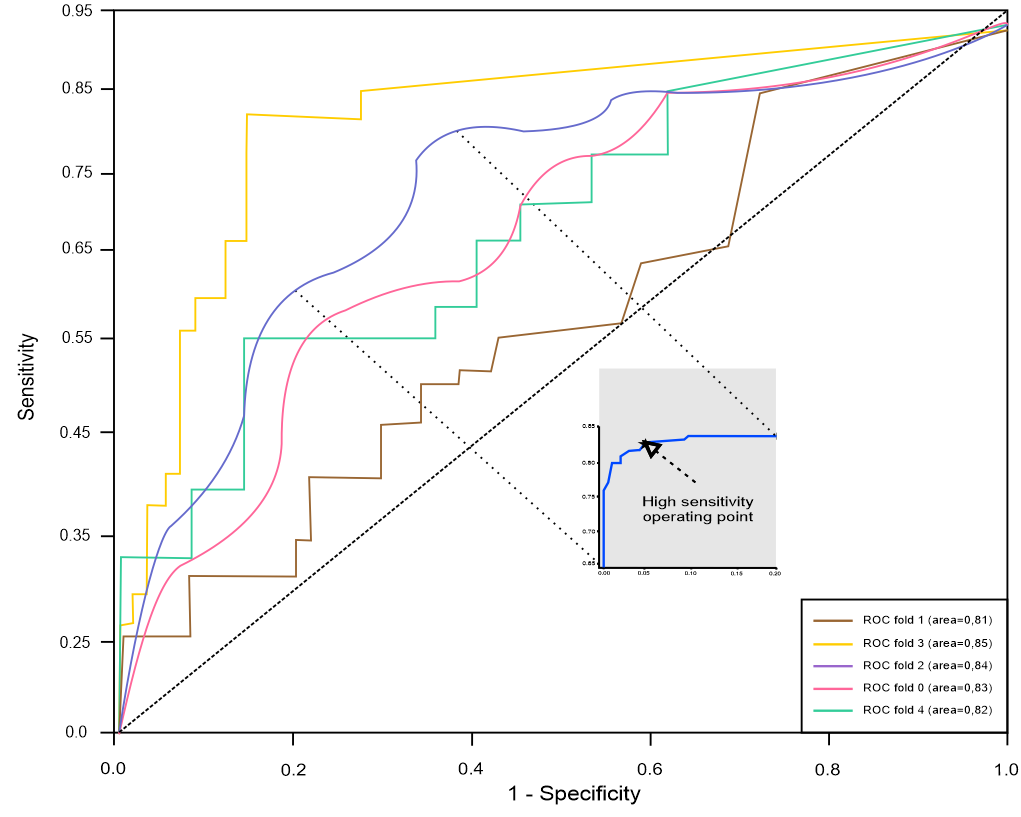
\includegraphics[width=0.9\linewidth]{images/roc_pgr.png}
		\caption{PGR status classification}
        \label{fig:pgr_roc}
	\end{subfigure}\\[1ex]
	\begin{subfigure}{0.49\linewidth}
		\centering
		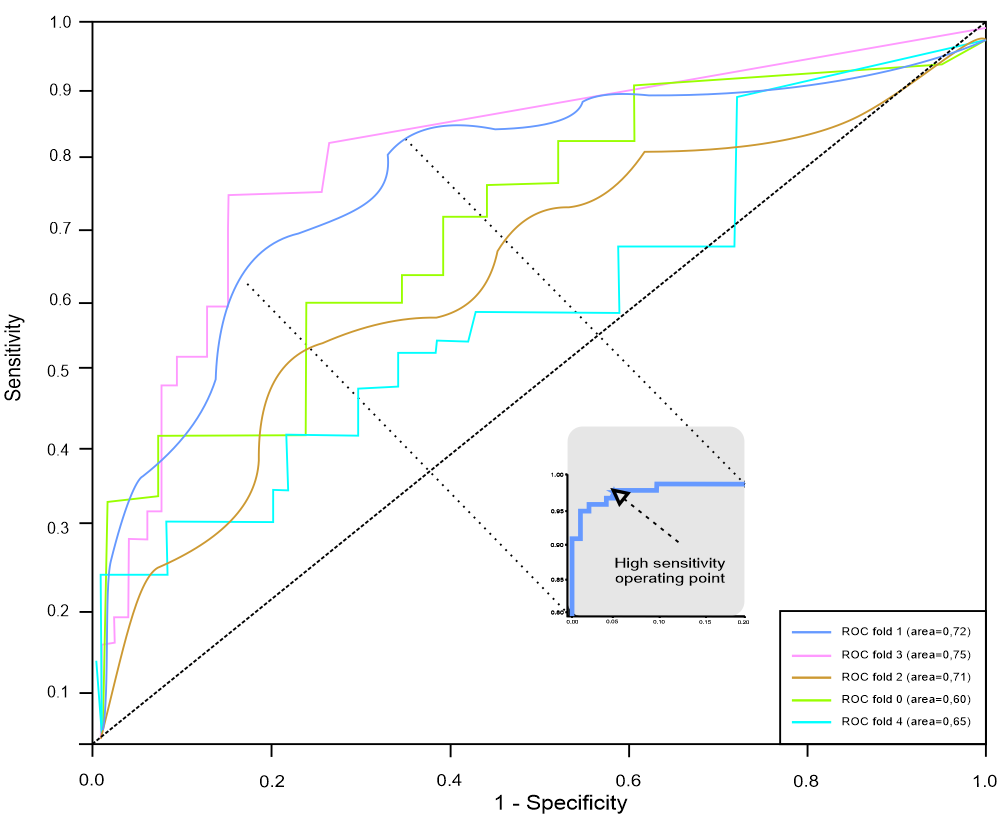
\includegraphics[width=0.9\linewidth]{images/roc_her2.png}
		\caption{HER2 status classification }
        \label{fig:her2_roc}
	\end{subfigure}
	\caption{ROC curve of the best predictor for ER, PGR, and HER2 status classification~\cite{karimACCESS2019}} 
	\label{fig:roc_all}
\end{sidewaysfigure*}

\subsection{Analysis of subtype classification}
The best results for ER status prediction are shown in in~\cref{tab:all_results} for each modality, where a combined input of GE and miRNA expression data performs the best than any single input modality. The confusion matrix in~\cref{fig:er_confusion} shows predictions about 288 breast cancer patients in which 197 were `ER Positive', 58 where `ER Negative', and 33 samples for `ER Indeterminate'. Out of 197 samples, the classifier classified 187 `ER Positive' cases correctly, making only 10 mistakes~(misclassification) in which 3 were misclassified as `ER Negative' and 7 of them were classified as `ER Indeterminate', giving overall high model confidence. 

\begin{table}[h]
    \centering
    \footnotesize
    \caption{Top results for ER, PGR, and HER2/neu status classification~\cite{karimACCESS2019}}
    \vspace{-2mm}
    \label{tab:all_results}
    \begin{tabular}{l|l|l|l|l|l} 
        \hline
        \textbf{Tasks} & \textbf{Input modality} & \textbf{MCC} & \textbf{Precision} & \textbf{Recall} & \textbf{F1} \\ 
        \hline
         & DNA methylation   & 0.7573 & 0.8948    & 0.8969 & 0.8958  \\ 
        \cline{2-6}
            & Gene expression  & 0.7745 & 0.8944    & 0.9004 & 0.8964  \\ 
        \cline{2-6}
        ER status       & miRA expression & 0.7235 & 0.8846    & 0.8876 & 0.8857  \\ 
        \cline{2-6}
                      & Gene + miRNA expression  & 0.7928 & 0.9325    & 0.9336 & 0.932   \\ 
        \cline{2-6}
                   & Gene + miRNA expression + DNA methylation & 0.7876 & 0.9175    & 0.918  & 0.9177  \\ 
        \hline
                     & DNA methylation   & 0.6963 & 0.7849    & 0.7939 & 0.7877  \\ 
        \cline{2-6}
                       & Gene expression  & 0.7134 & 0.8166    & 0.8276 & 0.8174  \\ 
        \cline{2-6}
        PGR status  & miRA expression   & 0.7059 & 0.7717    & 0.7743 & 0.7672  \\ 
        \cline{2-6}
                     & Gene + miRNA expression   & 0.7456 & 0.8566    & 0.8633 & 0.856   \\ 
        \cline{2-6}
                     & Gene + miRNA expression + DNA methylation & 0.7791 & 0.7987    & 0.8086 & 0.8001  \\ 
        \hline
                    & DNA methylation   & 0.5632 & 0.376     & 0.613  & 0.466   \\ 
        \cline{2-6}
                     & Gene expression   & 0.5967 & 0.6355    & 0.607  & 0.6173  \\ 
        \cline{2-6}
        HER2/neu status & miRA expression  & 0.6124 & 0.5627    & 0.5885 & 0.5732  \\ 
        \cline{2-6}
                   & Gene + miRNA expression   & 0.6276 & 0.6207    & 0.6444 & 0.627   \\ 
        \cline{2-6}
                   & Gene + miRNA expression + DNA methylation & 0.5743 & 0.3368    & 0.5804 & 0.4263  \\
        \hline
    \end{tabular}
    \vspace{-2mm}
\end{table}

\hspace*{3.5mm} Furthermore, as shown in the ROC curve in~\cref{fig:er_roc}, AUC scores for class 0, 1, and 2 are 0.91, 0.89, and 0.94, respectively, albeit we had only a few `Indeterminate' samples in the test set. The best results of PGR status prediction for each type of input is shown in~\cref{tab:all_results}. Similar to ER status prediction task, the predictor performs the best with the input of GE data combined with miRNA expression data. The other predictor with combined input of DNA methylation + gene expression + miRNA expression also performs relatively well. Best results are highlighted in green in~\cref{tab:all_results}. As seen from the confusion matrix in~\cref{fig:pgr_confusion}, the model is evaluated on 263 samples in which 167 were `PGR Positive', 75 `PGR Negative', and only 21 `PGR Indeterminate'. The best result was observed with the GE + miRNA expression input modality. As seen from~\cref{fig:pgr_roc}, AUC score for class 0~(`PGR Positive') and class 1~(`PGR Negative') are both 0.79, while 0.86 for class 2~(`PGR Indeterminate').

\begin{figure*}[h]
	\centering
	\begin{subfigure}{.49\linewidth}
		\centering
		\includegraphics[width=0.9\linewidth,height=50mm]{images/conf_er.png}
		\caption{ER status classification}
        \label{fig:er_confusion}
	\end{subfigure}
	\begin{subfigure}{.49\linewidth}
		\centering
		\includegraphics[width=0.9\linewidth,height=50mm]{images/conf_pgr.png}
		\caption{PGR status classification}
        \label{fig:pgr_confusion}
	\end{subfigure}\\[1ex]
	\begin{subfigure}{0.49\linewidth}
		\centering
		\includegraphics[width=0.9\linewidth,height=50mm]{images/conf_her2.png}
		\caption{HER2 status classification }
        \label{fig:her2_confusion}
	\end{subfigure}
	\caption{Confusion matrix for ER, PGR and HER2 status classification~\cite{karimACCESS2019}} 
	\label{fig:multi_cms}
\end{figure*}

%\subsubsection{Breast cancer subtype classification (HER2/neu status)}
\hspace*{3.5mm} The best results for HER2/neu status prediction for each type of input is shown in \cref{tab:all_results}. Similar to the ER and PGR status prediction tasks, the predictor performs the best with the input of GE data combined with miRNA expression data.  However, we observed overall a low accuracy score for each type of data, although, the performance on the training set itself was near to perfect. Even after applying several regularization techniques such as l2-regularization and Gaussian dropout layers, the result is still poor, which might be because of the overfitting. One of the possible causes for such overfitting is the smaller number of samples~(i.e. 860 samples) compared to ER and PGR statuses~(i.e. 1,024 samples).

\begin{figure*}
	\centering
	\begin{subfigure}{.49\linewidth}
		\centering
		\includegraphics[width=0.9\linewidth,height=50mm]{images/1.png}
		\caption{ER status classification}
        \label{fig:top_er}
	\end{subfigure}
	\begin{subfigure}{.49\linewidth}
		\centering
		\includegraphics[width=0.9\linewidth,height=50mm]{images/2.png}
		\caption{PGR status classification}
        \label{fig:top_pgr}
	\end{subfigure}
	\begin{subfigure}{0.49\linewidth}
		\centering
		\includegraphics[width=0.9\linewidth,height=50mm]{images/3.png}
		\caption{HER2 status classification }
        \label{fig:top_her2}
	\end{subfigure}
	\caption{Top ER, PGR, and HER2 status classifications results for each input type~\cite{karimACCESS2019}} 
	\label{fig6}
		\vspace{-4mm} 
\end{figure*}

\begin{figure*}[h]
	\centering
	\begin{subfigure}{.48\linewidth}
		\centering
		\includegraphics[width=0.9\linewidth,height=55mm]{images/raw_tsne.png}
		\caption{t-SNE plot of raw gene expression}
        \label{fig:tsne_raw}
	\end{subfigure}
	\begin{subfigure}{0.48\linewidth}
		\centering
		\includegraphics[width=0.9\linewidth,height=55mm]{images/ae_tsne.png}
		\caption{t-SNE plot of encoder's latent feature}
        \label{fig:tsne_ae}
	\end{subfigure}
	 \setlength{\belowcaptionskip}{-8pt}
	\caption{t-SNE visualization of gene expressions vs autoencoder latent feature map~\cite{karimACCESS2019}} 
	\label{fig:tnse}
	\vspace{-4mm}
\end{figure*}

\hspace*{3.5mm} The best result based on gene + miRNA expression modality is highlighted in green in~\cref{tab:all_results}, while the corresponding confusion matrix is shown in~\cref{fig:her2_confusion}. As seen, the predictor is evaluated on 225 samples, with 40 of them actually `HER2/neu Positive', 121 of them are `HER2/neu Negative', 21 of them are `HER2/neu Indeterminate', and 32 of them are `HER2/neu Equivocal' in this test set. The classifier correctly predicted 173 `HER2' cases, making 48 mistakes showing overall low confidence giving about 80\% accuracy. Furthermore, the ROC curve of this experiment is shown in~\cref{fig:her2_roc}. As observed, with 2 out of 4 classes achieve lower than 0.5 AUC score: the AUC score for class 0 (`HER2/neu Positive') is 0.83, for class 1 (`HER2/neu Negative') is 0.73, for class 2~(`HER2/neu Indeterminate') is 0.36, and for class 3~(`HER2/neu Indeterminate') is 0.48. 

\hspace*{3.5mm} Further, inspired from literature~\cite{rhee2017hybrid} and to qualitatively study whether the learned representation can express biological characteristics of the patients, t-SNE of the MAE encoder's output i.e. latent feature map and the t-SNE plot with raw GE are plotted in \cref{fig:tnse}. We can observe moderately high distinctive patterns between three subtype patients. Since, all the input modality has high dimension, we consider the association between each feature. 

\iffalse
\subsection{Consistency of subtype prognosis}
Inspired from literature~\cite{rhee2017hybrid} and to qualitatively study whether the learned representation can express biological characteristics of the patients, t-SNE of the MAE encoder's output i.e. latent feature map and the t-SNE plot with raw GE are plotted in \cref{fig:tnse}. We can observe moderately high distinctive patterns between three subtype patients. Since, all the input modality has high dimension, we consider the association between each feature. 

\begin{figure*}[h]
	\centering
	\begin{subfigure}{.48\linewidth}
		\centering
		\includegraphics[width=0.9\linewidth,height=55mm]{images/raw_tsne.png}
		\caption{t-SNE plot of raw gene expression}
        \label{fig:tsne_raw}
	\end{subfigure}
	\begin{subfigure}{0.48\linewidth}
		\centering
		\includegraphics[width=0.9\linewidth,height=55mm]{images/ae_tsne.png}
		\caption{t-SNE plot of encoder's latent feature}
        \label{fig:tsne_ae}
	\end{subfigure}
	 \setlength{\belowcaptionskip}{-8pt}
	\caption{t-SNE visualization of gene expressions vs autoencoder latent feature map~\cite{karimACCESS2019}} 
	\label{fig:tnse}
\end{figure*}

\hspace*{3.5mm} Further, we can see that the order of subtypes in the t-SNE plot is identical to prognosis of breast cancer subtypes. Research~\cite{91Caruana} has exposed that 80\% of all breast cancers are `ER-positive' in which the cancer cells grow in response to the hormone estrogen. While about 65\% of these are also `PR-positive' in which the cancer cells grow in response to another hormone, progesterone. ER/PR-positive tumors are much more likely to respond to hormone therapy than tumors that are ER/PR-negative. In about 20\% of breast cancers, the cells make too much HER2 protein and tend to be aggressive and fast-growing\footnote{\url{https://www.webmd.com/breast-cancer/}}. In breast cancer, certain subtype has the worst prognosis e.g. basal, followed by HER2, Luminal B, and Luminal A. The reason is that basal subtype has distinctive molecular characteristics from other subtypes~\cite{bertucci2012basal}. However, not all these patterns clearly visible in the t-SNE plot with raw GE, which signifies that the MAE learned the latent molecular properties better from the patient expression profiles.

\subsection{Survival analysis}
\label{secExperimentationAndResults_ResRegression}
Similar to breast cancer subtype prediction, survival rate prediction task is performed with multi-type inputs. Best results for each type of input are shown in~\cref{tab:sur_results}, in which the overall lowest $MSE$ was recorded with the gene expression modality, although coefficient of the determination $R^2$ is negative. In case of DNA methylation + gene expression + miRNA expression modality, the MSE score is considerably high and the corresponding $R^2$ score is negative. These two cases indicates that the predictions are worse than the actual average output. In contrast, $R^2$ scores for the DNA methylation, miRNA expression, and gene expression + miRNA expression modalities are also positive, even though the corresponding MSE scores are lower than that of DNA methylation modality. Further, the $R^2$ is a positive value, which indicates it performs better than the actual average output. 

\begin{table}[h]
	\centering
	\caption{top results for survival rate prediction~\cite{karimACCESS2019}}
	\vspace{-3mm}
	\label{tab:sur_results}
	\begin{tabular}{l|c|c}
		\hline
		\multicolumn{1}{c|}{\textbf{Modality}}   & \textbf{MSE}  & \textbf{$R^2$}  \\ \hline
		DNA methylation & 0.26537  & 0.13054  \\ \hline
		Gene expression & {\color[HTML]{009901} 0.16541}  & -0.18753 \\ \hline
		miRNA expression & 0.34732 & 0.12468 \\ \hline
		\begin{tabular}[c]{@{}l@{}}Gene expression + miRNA expression\end{tabular}                     & {\color[HTML]{333333} 0.27615} & {\color[HTML]{009901} 0.19542}  \\ \hline
		\begin{tabular}[c]{@{}l@{}}DNA methylation + gene expression +\\ miRNA expression\end{tabular} & 0.57834 & -0.2735  \\ \hline
	\end{tabular}
\end{table}

\hspace*{3.5mm} To further evaluate the ability of the model to comprehend characteristics of molecular subtypes, we performed survival analysis inspired by literature~\cite{rhee2017hybrid}. We clustered the patients into two groups based on raw GE values and the MAE encoder's output i.e. latent feature map. K-means algorithm is used for the clustering and t-SNE is used for the dimension reduction and visualization. To the measure hazard ratios of different patient groups and to analyze the effectiveness of treatment by comparing the Kaplan-meier~(KM) plots (based on non-parametric statistics) of the treated and non-treated patient group are drawn for each of two clustering results as shown in~\cref{fig:km_sur_plot}.

\begin{figure*}[h]
	\centering
	\begin{subfigure}{.48\linewidth}
		\centering
		\includegraphics[width=\linewidth,height=60mm]{images/raw_cluster.png}
		\caption{KP plot of raw gene expression $p-value>0.05$}
        \label{fig:km1}
	\end{subfigure}
	\begin{subfigure}{0.48\linewidth}
		\centering
		\includegraphics[width=\linewidth,height=60mm]{images/ae_cluster.png}
		\caption{KP plot of latent feature $p-value<0.05$}
        \label{fig:km2}
	\end{subfigure}
	\caption{Kaplan meier survival plots of the patients~\cite{karimACCESS2019}} 
	\label{fig:km_sur_plot}
\end{figure*}

\hspace*{3.5mm} The plot generated by the latent features~(\cref{fig:km2}) shows that the patient samples are more clearly separated into two subgroups showing distinct survival patterns with a $p-value<0.05$, while the plot with raw expression value~(\cref{fig:km1}) failed giving $p-value>0.05$. This is an interesting result as it shows that the model can simultaneously learn the genotypic information of patient from multimodal input features while performing the classification task.

\subsection{Comparison with ML baselines}
Although our datasets are collected from TCGA, multimodal features are used to train DL algorithms. Nevertheless, none of the related works summarized in~\cref{table:stateofart} used multimodality for breast cancer subtypes. 
%and survival prediction. 
Thus, a one-to-one comparison in a DL setting was not viable. Instead, we created unimodal and multimodal features out of each input type and train LR, KNN, NB, SVM, RF, and GBT as ML baseline models classifiers. 
%On the other hand, linear regression~($\hat{LR}$), Support Vector Regression~(SVR), Gradient Boosted Regression~(GBR), and random forest regression~(RFR) models were trained for predicting survival rates. 
In this setting, hyperparameters optimization is performed using random search with 5-fold cross validation. 

\hspace*{3.5mm} As shown in \cref{table:classification} 
%and \cref{table:regression}
, the GBT and RF-based classifiers 
%and regression models 
perform consistently best for subtype classification. %and survival prediction. 
The classification analysis can be further validated by calibrating the best performing MAE classifier against different embedding methods for which the output probability of the classifier can be directly interpreted as a confidence level in terms of `fraction of positives'~(FOP) as shown in~\cref{fig:cal}. As seen the MAE classifier gave a probability value~(i.e. FOP) between 0.82 to 0.93, which means 93\% predictions belong to true positives, whereas the second best GBT and RF generates the FOP values between 0.75 to 0.87 and between 0.76 to 0.89, respectively. 

\begin{table}[htp!]
	\renewcommand{\arraystretch}{0.9}
	\caption{survival prediction with ML regressors~(*=modality with best results)~\cite{karimACCESS2019}}
	\label{table:regression}
	\scriptsize
	\vspace{-2mm}
	\centering
	\begin{tabular}{p{2.8cm}|l|r|r}
		\toprule
		\textbf{Modality} & \textbf{Regressor} & \textbf{MSE} & \textbf{$R^2$} \\ \hline
		\multirow{4}{*}{DM} & $\hat{LR}$ & 0.4523 & -0.5432 \\
		& SVR & 0.6536 & -0.1156 \\
		& GBR & 0.3431 & -0.0135\\
		& RFR & 0.2314 & 0.0153\\
		\hline
		\multirow{4}{*}{GE} & $\hat{LR}$ & 0.6754 & -0.2348 \\
		& SVR & 0.5437 & -0.1102  \\
		& GBR & 0.2373 & -0.0653 \\
		& RFR & 0.1765 & 0.1176 \\
		\hline
		\multirow{4}{*}{miRNA} & $\hat{LR}$ & 0.8674 & -0.7832  \\
		& SVR & 0.6134 & -0.4569  \\
		& GBT & 0.5762 & -0.1542 \\
		& RF & 0.2956 & 0.1342\\
		\hline
		\multirow{4}{*}{GE+miRNA} & $\hat{LR}$ & 0.3451 & -0.1578  \\
		& SVR & 0.3538 & -0.3486  \\
		& GBR & 0.1937 & 0.0954 \\
		& RFR & 0.1456 & 0.1185 \\
		\hline
		\multirow{4}{*}{DM+GE+miRNA} & $\hat{LR}$ & 0.6523 & -0.8981 \\
		& SVR & 0.7287 & -0.7541  \\
		& GBR & 0.5123 & -0.6541 \\
		& RFR & 0.3287 & -0.2485 \\
        \hline
	\end{tabular}
\end{table}

\begin{figure}[htp!]
	\centering
	\includegraphics[width=0.8\linewidth]{images/cali.png}	
	\caption{Calibrating different classifiers~\cite{karimACCESS2019}}	
	\label{fig:cal}
\end{figure}

\begin{sidewaysfigure}[htp!]
	\centering
	\begin{subfigure}{0.48\linewidth}
		\centering
		\includegraphics[width=0.9\linewidth,height=80mm]{images/SVM.png}
%		\includegraphics[width=\linewidth,height=40mm]{SVM.png}
		\caption{SVM}
		\label{fig9a}
	\end{subfigure}
	\begin{subfigure}{0.48\linewidth}
		\centering
		\includegraphics[width=0.9\linewidth]{images/GBT.png}
		\caption{GBT}
		\label{fig9b}
	\end{subfigure}
	\begin{subfigure}{0.48\linewidth}
		\centering
		\includegraphics[width=0.9\linewidth]{images/RF.png}
		\caption{RF}
		\label{fig9c}
	\end{subfigure}
	\begin{subfigure}{0.48\linewidth}
		\centering
		\includegraphics[width=0.9\linewidth]{images/MAE.png}
		\caption{MAE}
		\label{fig9d}
	\end{subfigure}
	\caption{Learning curves showing the validation and training scores of top-3 and SVM classifiers} 
	\label{fig:lc}
\end{sidewaysfigure}

\begin{table}
	\renewcommand{\arraystretch}{0.9}
	\caption{Subtypes prediction with ML classifiers~(*=modality with best results)~\cite{karimACCESS2019}}
	\label{table:classification}
	\vspace{-2mm}
	\scriptsize
	\centering
	\begin{tabular}{p{2.5cm}|l|r|r|r}
		\toprule
		\textbf{Modality} & \textbf{Classifier} & \textbf{Precision} & \textbf{Recall} & \textbf{MCC}\\ \hline
		\multirow{7}{*}{DM} & LR & 0.74 & 0.72 & 0.53 \\
		& NB & 0.73 & 0.70 & 0.55 \\
		& SVM & 0.80 & 0.81 & 0.69 \\
		& KNN & 0.69 & 0.71 & 0.51 \\
		& GBT & 0.88 & 0.85 & 0.72\\
		& RF & 0.91 & 0.92 & 0.75\\
		& \textbf{MAE}  & 0.93 & 0.91 & 0.79 \\
		\hline
		\multirow{7}{*}{GE} & LR & 0.76 & 0.72 & 0.59 \\
		& NB & 0.73 & 0.72 & 0.55 \\
		& SVM & 0.80 & 0.81 & 0.66 \\
		& KNN & 0.73 & 0.73 & 0.53 \\
		& GBT & 0.87 & 0.86 & 0.74\\
		& RF & 0.89 & 0.88 & 0.77\\
		& \textbf{MAE} & 0.92 & 0.91 & 0.79 \\ 
		\hline
		\multirow{7}{*}{miRNA} & LR & 0.75 & 0.73 & 0.54 \\
		& NB & 0.72 & 0.71 & 0.53 \\
		& SVM & 0.78 & 0.79 & 0.68 \\
		& KNN & 0.71 & 0.69 & 0.53 \\
		& GBT & 0.87 & 0.85 & 0.71\\
		& RF & 0.89 & 0.86 & 0.73\\
		& \textbf{MAE} & 0.89 & 0.90 & 0.75 \\ 
		\hline
		\multirow{7}{*}{GE+miRNA*} & LR & 0.72 & 0.71 & 0.57 \\
		& NB & 0.69 & 0.70 & 0.51 \\
		& SVM & 0.75 & 0.74 & 0.64 \\
		& KNN & 0.63 & 0.59 & 0.49 \\
		& GBT & 0.83 & 0.82 & 0.69\\
		& RF & 0.84 & 0.85 & 0.71\\
		& \textbf{MAE} & 0.87 & 0.88 & 0.74 \\ 
		\hline
		\multirow{7}{*}{DM+GE+miRNA} & LR & 0.65 & 0.68 & 0.47 \\
		& NB & 0.70 & 0.71 & 0.50 \\
		& SVM & 0.72 & 0.73 & 0.55 \\
		& KNN & 0.69 & 0.66 & 0.52 \\
		& GBT & 0.81 & 0.82 & 0.65\\
		& RF & 0.82 & 0.83 & 0.66\\
		& \textbf{MAE} & 0.84 & 0.85 & 0.69 \\
        \hline
	\end{tabular}
\end{table}

\hspace*{3.5mm} When it comes to survival prediction with ML regression models, the lowest $MSE$ was recorded with the gene expression modality using GBR regression model but much higher than that of MAE-based one. Whereas, the coefficient of determination $R^2$ is a positive value. In case of DNA methylation + gene expression + miRNA expression modality, the MSE score is considerably high and the corresponding $R^2$ score is also negative. These two cases indicates that the predictions are worse than the actual average output. On the other hand, $R^2$ scores for the miRNA expression, and gene expression + miRNA expression modalities are also positive but lower than that ones generated by MAE, even though the corresponding MSE scores are much higher than that of ones generated with MAE. In summary, the gene expression + miRNA expression modality shows the highest $R^2$  and lowest MSE score, which indicates it performs better than the actual average output showing moderately worse performance than that of MAE. 
\fi 

\subsection{Discussion}\label{chapter_4:discussion}
Overall the best results for breast cancer subtypes classification~(ER, PGR, and HER2 status) is generated from the MAE implementation with the input of GE and miRNA expression data, which is the best results for individual classification tasks. The HER2 status classification got the worst results by far compared to ER and PGR status ones, which is probably because the HER2 status data has fewer samples than ER and PGR ones. The training accuracy for each classifier far exceeds the test accuracy, probably because of overfitting. One reason is lack of training samples. As shown in~\cref{fig6}, the number of samples across datasets is only 1,000. While, the smallest number of feature~(e.g. 1,881 features in miRNA expression) still exceeds it, where the number of features in DNA methylation and GE exceeds other modalities. 
%In contrast, we experience varying results on survival prediction, e.g. AE achieves the lowest MSE score with the input of DNA methylation but giving a negative $R^2$ score, which means the prediction itself is not better than the average of the actual output. Positive $R^2$ scores were achieved with miRNA expression and GE + miRNA expression inputs using AE and MAE, respectively. To understand the effects of having more training samples, and to understand whether our classifiers suffer more from variance errors or bias errors, we observed the learning curves of top-3 classifiers~(i.e., RF, GBT, and MAE) and SVM~(a linear model) for varying numbers of training samples.

\hspace*{3.5mm} In our initial experiments, we observed by training ML models. For SVM the validation and training scores converge to a low value with increasing size of the training set. Consequently, SVM did not benefit much from more training samples. However, RF and GBT are tree-based ensemble methods, and the MAE model can learn more complex concepts from the GE + miRNA multimodal features. This results in a lower bias, which can be observed from higher training scores than the validation scores for the maximum number of samples i.e. adding more training samples does increase model generalization. Overall, MAE gave relatively better results compared to regular AE with a single type of input.
%as well as other best ML baselines, e.g., GBT and RF. 
It mostly occurs with the GE + miRNA expression giving the best results for subtypes classification.
%and decent results for survival rate prediction. 
Based on this comparison, we can conclude that there is a possibility MAE might surpass AE and ML baselines models such as GBT or RF performance with the right combination of inputs. 

\section{Chapter Summary}\label{chapter_4:conclusion}
In this paper, we developed a clin ical DSS, which is technically based on an MAE for predicting different subtypes of breast cancer patients.
%and their survival rates. 
Experiment results for the subtype classification are promising, especially based on the ER and PGR status having 0.93 F1-score, which produced with combined inputs of GE and miRNA expression data. 
%The performance result of the survival rate prediction shows varying signs. The best $MSE$ score is taken from predictors with DNA methylation as an input, although the $R^2$ score itself is negative, which indicate that it still performs worse than the simple average output. The GE + miRNA expression combination data as input gave very good results in general, although it did not have the best performance on the survival rate prediction.
However, the overall decision accuracy of DSS is hindered due to several factors: i) limited amount of labeled genomics data, which is probably individual patients privacy. This limitation causes of overfitting while training our neural network. 

\hspace*{3.5mm} The training scores is much higher than the validation scores for the maximum number of samples i.e. adding more training samples does increase model generalization. This suggest that the prediction can be made more confidently if we had more labelled training data, ii) secondly, we did not perform any feature selection but let the network to choose from the very high dimensional inputs. Consequently, for some input combinations the pretraining error for the MAE were getting out of bound, ii) limited amount of publicly available genomics data sources because other sources such as ICGC and COSMIC are not comprehensive even requiring restricted access. The DSS based on multimodal data is black-box, hence lack of interpretability. However, interpretability is important to gain insights into the reasons why a given cancer case is of a certain type can help in finding more accurate treatments and drug repositioning. Further, the ``right to explanation'', of EU GDPR~\cite{kaminski2019right} gives patients the right to know why and how an algorithm makes a diagnosis decision. 
%In the future, we intend to develop a more robust multimodal network such as multimodal Convolutional-LSTM to act both feature extractor and classifier and train with an enriched number of samples from other sources to develop an explainable deep architecture might open future opportunity to learn more towards potential gene set biomarkers based diagnosis. 

\hspace*{3.5mm} In the next chapter, we extend both single and multimodality-based cancer typing methods to overcome both limitations. We increase the number of samples, by combining samples from the PanCancerAtlas. We will focus on improving the explanations of the predictions using both ante-hoc approach by seeding explainability into the model from the beginning, to learn more towards potential gene set biomarkers based diagnosis. Further, to identify significant biomarkers, we will generate class-specific heat maps using guided-gradient class activation maps++~(Grad-CAM++) and layer-wise relevance propagation~(LRP). We will compute feature importance in terms of mean absolute impact, followed by ranking top genes across all the cancer types. Finally, we will provide explanations of the predictions.  
%In particular, we will focus on multimodality with reversed time attention model and Bayesian deep learning~\cite{choi2016retain}. 

\chapter{Interpreting Black-box Models}\label{chapter:xai}

\textit{"Predicting the future isn't magic, it's artificial intelligence."} -- Dave Waters 

\section{Chapter Overview}
In chapter \ref{chapter:uni_modality} and \ref{chapter:multiodality}, different modalities were considered to develop decision support system~(DSS) to leverage cancer types and subtypes prediction tasks. In both cases, the predictive models developed are mostly black-box methods. However, not only accurate diagnosis ~(i.e., predicting cancer types), but also revealing and interpreting biological significance about driver genes are vital for subsequent treatment. 

Besides, since data subjects are entitled to obtain meaningful information about logic, significance, and envisaged impacts of automated decision making, it is important to improve algorithmic transparency of the model based on which a DSS will be built upon. To improve the algorithmic transparency and explainability of the black-box models, different probing and interpretable methods are applied. Further, we validated our findings through functional analysis to make sure biomarkers are biologically trustworthy

\section{Introduction}\label{chapter_5:intro}
As the importance of genetic knowledge in cancer treatment is increasingly addressed, several projects have emerged, of which TCGA most well-known for omics data. Omics data is a collection of biomolecules inside living things such as genomics, metabolomics, and proteomics. TCGA curates various omics data, e.g., mutations, GE, DNA methylation, CNV, and miRNA expressions. By acquiring deep insights of these data, treatment can be focused on preventive measures. Besides, clinical and pathology information are provided. TCGA further analyzed over 11,000 cancer cases from 33 prevalent forms of cancer, which fostered the accomplishment of the Pan Cancer Atlas~(PCAt) project, covering gene expression, somatic mutation, DNA methylation, miRNA expression, and CNV~\cite{lyu2018deep}. 

\hspace*{3.5mm} In this chapter, multimodal genomics data is used to train deep neural network~(DNN) architectures to classify the cohorts into specific cancer patient groups. In particular, data from PCAt project~\cite{weinstein2013cancer} is used to train deep neural network~(DNN) architectures to classify the cohorts into specific cancer patient groups. In particular, a vanilla convolutional neural network~(CNN) and deep CNN architecture called VGG-16 are trained end-to-end for the classification. On the other hand, multimodal autoencoder~(MAE) and multimodal convolutional autoencoder~(MCAE) networks are to trained to learn joint latent representation from the multimodal genomics data before the classification.  
Diagnoses provided by the DSS consist of three steps: i) classifying cohort(s)~(group and individual) into specific cancer types based on their respective profiles, and ii) interpreting the prediction by highlighting biologically relevant biomarkers, and iii) explaining necessary logic involved in the diagnosis. These steps are based on two different strategies: based on single modality~(i.e., using single genomics data) and based on multimodality. %~(i.e., using different genomics data). 

\hspace*{3.5mm} To improve algorithmic transparency, different probing techniques are employed to open the `black-box' models. Since genomics data are high dimensional, we hypothesize\footnote{\textbf{H4}: \textit{Since genomics data is high dimensional, embedding them into 2D raw images can help locate significant~(i.e, most and least) biomarkers.}} that embedding them into 2D raw images can help locate significant~(i.e, most and least) biomarkers
\footnote{Supporting publication: \textbf{Md. Rezaul Karim}, Michael Cochez, Oya Beyan, Stefan Decker, and Christoph Lange-Bever, ``OncoNetExplainer: Explainable Predictions of Cancer Types Based on Gene Expression Data", Proc. of \emph{IEEE International Conference on Bioinformatics and Bioengineering~(BIBE'2019)}, Athens, Greece, October 28-30, 2019}. % for the corresponding tumor types. 
To identify relevant biomarkers\footnote{RQ2: \textit{How to identify relevant features or factors for a certain decision?}}, GradCAM++, attention mechanism, and LRP are used to generate class-specific heat maps~(HM) for all classes. 
Marker genes w.r.t prominent pixels position on 2D feature space are then marked, followed by computing their  importance in terms of mean absolute impact~(MAI). Top-k genes across cancer types are also ranked w.r.t MAI, followed by their functional analyses.  

%\footnote{Algorithmic transparency, w.r.t, post-model explainability.}. 
%Further, we validated our findings through functional analysis to make sure biomarkers are biologically trustworthy

\hspace*{3.5mm} The rest of the chapter is structured as follows: \cref{chapter_5:rw} covers related works concerning interpretable ML approaches and summarize their potential limitations. \Cref{chapter_5:mm} describes the overall approach, including the detail of the data collection and feature engineering before the network construction and training. \Cref{chapter_5:results} demonstrates the experiment results and discusses key findings of the study. \Cref{chapter_5:conclusion} provides explanations of the importance and relevance of the study reported, highlights the limitations and discuss future works before concluding the chapter.

\section{Related Work}\label{chapter_5:rw}
Lyu et al.~\cite{lyu2018deep} and Mostavi et al.~\cite{mostavi2019convolutional} embedded the RNA-Seq data from the PCA project into 2D images and trained a CNN to classify 33 tumor types, which outperforms the approach in~\cite{li2017comprehensive}. Besides, they provide a functional analysis of genes with high intensities in the HM based on Grad-CAM and validated that these top genes are related to tumor-specific pathways. Other general methods on explainability, fairness and robustness. 
%There is no prior art that handles a diverse set of desirable properties needed to develop a responsible AI system. 
Several other works introduced counterfactual explanations. However, their optimization formulation cannot handle categorical data~\cite{ying2019gnnexplainer}, i.e, optimization does not solve for such data and the values are found in a brute-force fashion.

\hspace*{3.5mm} \Cref{tab:multimodal_xai_approaches} and \cref{tab:global_vs_lical_xai} show the summarized views of the methods focusing interpretability, explainability, and transparency. Some other explainable methods works only for the linear models. Other approaches use a genetic algorithm to generate neighbors around the input and then use decision trees to locally approximate the model. However, local approximations might be at the cost of model accuracy, and they define counterfactual based on the minimum number of splits in the trained decision tree, which might not always be the smallest change to the input~\cite{li2017comprehensive}. They work on a white-box and simpler convolution models, and the distance metrics might not be apt to measure image similarity. 

\begin{table}[h]
    \centering
    \caption{XAI approaches w.r.t algorithmic fairness, robustness, and explainability on agnosticism}
    \label{tab:multimodal_xai_approaches}
    \scriptsize
    \vspace{-2mm}
    \begin{tabular}{l|l|l|l|l|l|l} 
        \hline
        \textbf{Reference}                & \textbf{Multimodality support} & \textbf{Black-box} & \textbf{Agnostic} & \textbf{Explainability} & \textbf{Fairness} & \textbf{Robustness}  \\ 
        \hline
        Shubham S. et al. 2019   & Yes                   & Yes       & Yes            & Yes            & Yes      & Yes         \\ 
        \hline
        Wacherer et al. 2019     & Yes                   & Yes       & No             & Yes            & Yes      & No          \\ 
        \hline
        Ustun et al. 2019        & No                    & Yes       & Yes            & Yes            & Yes      & No          \\ 
        \hline
        Russel et al. 2019       & Yes                   & Yes       & No             & Yes            & Yes      & No          \\ 
        \hline
        Ribeiro et al. 2016      & Yes                   & Yes       & Yes            & Yes            & No       & No          \\ 
        \hline
        Guidtit et al. 2016      & Yes                   & Yes       & Yes            & Yes            & No       & No          \\ 
        \hline
        Carlini \& Wagner, 2017 & No                    & No        & Yes            & No             & No       & Yes         \\ 
        \hline
        Weng et a. 2018          & No                    & No        & Yes            & No             & No       & Yes         \\ 
        \hline
        Karim et al. 2019        & No                    & Yes       & Yes            & Yes            & Yes      & No          \\
        \hline
    \end{tabular}
    \vspace{-4mm}
\end{table}

\hspace*{3.5mm} A few other approaches define a robustness score that need to have access to the model gradients. GNNExplainer is a recent approach for explaining the predictions by a graph neural network~(GNN)~\cite{ying2019gnnexplainer}. Given a trained GNN model and an input instance, GNNExplainer can generate the explanations via a dense subgraph. Secondly, GNNExplainer can be applied across tasks, e.g., node classification, graph classification, and link prediction, in a task-agnostic way. Thirdly, GNNExplainer can be employed on different GNN models such as GCN, GraphSAGE, GAT, and SGC to generate corresponding explanations. 

\begin{table}[h]
    \centering
    \scriptsize
    \caption{Approaches to interpretability of ML models based on agnosticism}
    \label{tab:global_vs_lical_xai}
    \vspace{-2mm}
    \begin{tabular}{l|l|l} 
        \hline
        \textbf{Agnosticism}  & \textbf{Global interpretability}  & \textbf{Local interpretability} \\ 
        \hline
        \multirow{4}{*}{Model specific} & Regression (logistic/linear) models & Individual (e.g., patient) specific set of decision rules \\ 
        \cline{2-3}
        & Decision trees & Tree decomposition of decision rules \\ 
        \cline{2-3}
        & Naïve Bayes & K-nearest neighbour (KNN)\\ 
        \cline{2-3}
        & GNN Explainer~\cite{GNNEXPLAINER} & GNN Explainer~\cite{GNNEXPLAINER} \\ 
        \hline
        \multirow{5}{*}{Model agnostic} & Global surrogate models  & Local interpretable model-agnostic explanation (LIME)~\cite{LIME}\\ 
        \cline{2-3}
        &  MUSE  & Shapely additive explanations (SHAP)~\cite{SHAP}\\ 
        \cline{2-3}
        & Partial dependence plots (PDP) & Anchors~\cite{ribeiro2018anchors} \\ 
        \cline{2-3}
        & Summary plot showing global feature importance & MUSE \\ 
        \cline{2-3}
        & BETA~\cite{BETA} & Sailency and attention maps (e.g., CAM)\\ 
        \hline
    \end{tabular}
    \vspace{-4mm}
\end{table}

\hspace*{3.5mm} Due to the stochastic nature of DNN, the prediction and feature importance generated would be slightly different across runs, i.e., not deterministic. This also applied to DSS we developed in the previous chapters. We might even encounter similar issue for tree-based ensemble models such as random forest. For example, GBT provides 3 options for measuring feature importance: i) \emph{weight}, which is the number of times a feature is used to split the data across all trees, ii) \emph{cover}, the number of times a feature is used to split the data across all trees weighted by the number of training data points go through those splits, and iii) \emph{gain}, which is the average training loss reduction gained when using a feature for splitting. Based on these measure, feature importance orderings~(i.e., the order in which features were added) are different since subsequent features will get a disproportionately high weight.

\section{Methods}\label{chapter_5:mm}
In this section, we discuss our approach in detail, including data collection, preprocessing, network construction, and training, followed by interpreting the network towards biomarkers identification. There is no single approach to explainable AI that always works best~\cite{arya2019one}. There are many ways to explain an algorithmic decision or a model. The appropriate choice depends on the persona of the consumer and the requirements of the AI pipeline that bridge the gap from research to practice~\cite{arya2019one}. Based on this insights, we rely on several probing and interpretability methods discussed in \cref{chapter:preli}

\subsection{Problem statement}
From given genomics profiles of PCAt cohorts consisting of GE, DNA methylation, and miRNA expressions, the problem is to classify the patients into specific cancer types. Given $n$ samples, $X$ = ${{\{x_1,x_2, ..., x_n}}\}$ in dataset $D$, where $X \in {R}^{D}$. We consider classifying an individual $x$ into a specific cancer type based on its respective profiles, but in two different ways: i) based on single modality, ii) based on multimodality, where a  classifier is a function $f: {X}^{(m)} \rightarrow {Y}$, which maps a data instance $x$ from a feature space ${X}^{(m)}$ with $m$ input features to a labels $y$ in a target space ${Y}$, where $f(x)=y$ denotes the decision $y$ predicted by $f$, and input instance $x$ consists of a set of $m$ attribute-value pairs $\left(a_{i}, v_{i}\right)$ in which $a_i$ is a feature and $v_i$ is a value from the domain of $a_i$. 

\hspace*{3.5mm} In \cref{chapter:uni_modality}, we developed two `black-box' predictors: let's say $F$ is the first predictor whose internal functioning is either unknown to the observer or they are known but not interpretable by a human. In this chapter, we assume $F$ lacks of explainability by default, in which we embed local and global explainability logic to make it interpretable, which we hope to explain a data point $x$ using an explanation function $g$. We denote ${F}$ - an interpretable predictor, whose internal processing yielding a decision ${F}(x)=y$ can be given a symbolic interpretation understandable by a human. 

\hspace*{3.5mm} While using single modality, we classify samples directly in it's original data space $X$. In the latter approach, instead of classifying samples directly in it's original data space $X$, we first transform each data with a nonlinear mapping $f_{\theta}: X \rightarrow Z$, where $\theta$ are learnable parameters and $Z \in {R}^{K}$ is the learned or embedded feature space, where $K \ll D$. Then we create a shared representation of class-discriminating features from each modality, followed by parametrizing $f_{\theta}$ by representation learning based on multimodal convolutional autoencoders~(MCAE) is employed due to it's function approximation properties and feature learning capabilities~\cite{xie2016unsupervised,karim2019drug} from genomic data. Based on embedding $Z$, the classifier then $f$ maps an input $x$ to an output $f(x) \in y, f: {R}^{d} \mapsto y$. When we assume $f$ has a parametric form, we write $f_{\theta}$, where ${L}(f(x), y)$ denotes the loss function used to train $f$ on a dataset $D$ of input-output pairs $(x(i), y(i))$. Local explainability refers to an explanation for why $f$ predicted $f(x)$ for a fixed point $x$. 
%The local explanation methods we discuss come in one of the following forms: which feature $x_i$ of $x$ was most important for prediction with $f$? Which training data point $Z \in \mathbb{R}^{K}$ was most important to $f(x)$? What is the minimal change to the input $x$ required to change the output $f(x)$? 

\subsection{Datasets}
The DNA methylation, copy numbers, mutations, miRNA, and GE profiles from PCAt covering 33 prevalent tumor type for 9,074 samples are considered in our approach. This dataset has been used widely as prior knowledge to generate tumor-specific biomarkers~\cite{way2018machine,hoadley2018cell,malta2018machine}. These data are hybridized by the Affymetrix Genome-Wide Human SNP Array 6.0\footnote{\url{http://www.affymetrix.com/support/technical/byproduct.affx}}, which allows us to examine the largest number of cases along with the highest probe density~\cite{31Park}. Besides, we use the cancer transcriptomes from the PCAt project to interrogate GE states induced by deleterious mutations and copy number alterations. The sample distribution across data types are shown in \cref{table:alldatadetails2}~\cite{weinstein2013cancer}. 

\begin{table} [h]
\centering
    \scriptsize
    \caption{Sample distribution across tumor types: rows: tumour type, column: data types~\cite{weinstein2013cancer}}
    \label{table:alldatadetails2}
    \vspace{-2mm}
    \begin{tabular}{l|l|l|l|l|l|l}
        \hline
        \rowcolor{Gray}
         \textbf{Cohort} & \textbf{DNA meth.} & \textbf{Copy numbers} & \textbf{Mutations} & \textbf{miRNA} & \textbf{Gene expr.} & \textbf{Carcinoma type} \\\hline
            LUSC & 358 & 345 & 178 & 332 & 227 & Lung squamous cell carcinoma \\\hline
            READ & 162 & 164 & 69 & 143 & 71 & Rectum adeno-carcinoma \\\hline%
            GBM  & 405 & 578 & 290 & 501 & 495 & Glioblastoma multiforme \\\hline
            LAML & 194 & 198 & 197 & 187 & 179 & Acute myeloid leukemia	\\\hline%
            HNSC & 310 & 310 & 277 & 309 & 303 & Head \& neck squamous cell carcinoma \\\hline 
            BLCA & 126 & 126 & 99 & 121 & 96 & Bladder urothelial carcinoma \\\hline 
            KIRC & 457 & 457 & 417 & 442 & 431 & Kidney renal clear cell carcinoma  \\\hline
            UCEC & 512 & 511 & 248 & 497 & 333 & Uterine corpus endometrial carcinoma \\\hline
            LUAD & 431 & 357 & 229 & 365 & 355 & Lung adenocarcinoma \\\hline
            OV   & 592 & 577 & 316 & 454 & 581 & Ovarian serous cystadenocarcinoma \\\hline
            BRCA & 888 & 887 & 772 & 870 & 817 & Breast invasive carcinoma  \\\hline
            COAD & 420 & 422 & 155 & 407 & 192 & Colon cdenocarcinoma \\\hline
            LAML & 194 & 198 & 197 & 187 & 179 & Acute myeloid leukemia	\\\hline%
            HNSC & 310 & 310 & 277 & 309 & 303 & Head \& neck squamous cell carcinoma \\\hline 
            BLCA & 126 & 126 & 99 & 121 & 96 & Bladder urothelial carcinoma \\\hline 
            KIRC & 457 & 457 & 417 & 442 & 431 & Kidney renal clear cell carcinoma  \\\hline
            UCEC & 512 & 511 & 248 & 497 & 333 & Uterine corpus endometrial carcinoma \\\hline
            LUAD & 431 & 357 & 229 & 365 & 355 & Lung adenocarcinoma \\\hline
            OV   & 592 & 577 & 316 & 454 & 581 & Ovarian serous cystadenocarcinoma \\\hline
            BRCA & 888 & 887 & 772 & 870 & 817 & Breast invasive carcinoma  \\\hline
            COAD & 420 & 422 & 155 & 407 & 192 & Colon cdenocarcinoma \\\hline
            OV   & 592 & 577 & 316 & 454 & 581 & Ovarian serous cystadenocarcinoma \\\hline
            BRCA & 888 & 887 & 772 & 870 & 817 & Breast invasive carcinoma  \\\hline
            COAD & 420 & 422 & 155 & 407 & 192 & Colon cdenocarcinoma \\\hline
            LAML & 194 & 198 & 197 & 187 & 179 & Acute myeloid leukemia	\\\hline%
            HNSC & 310 & 310 & 277 & 309 & 303 & Head \& neck squamous cell carcinoma \\\hline 
            BLCA & 126 & 126 & 99 & 121 & 96 & Bladder urothelial carcinoma \\\hline 
            KIRC & 457 & 457 & 417 & 442 & 431 & Kidney renal clear cell carcinoma  \\\hline
            UCEC & 512 & 511 & 248 & 497 & 333 & Uterine corpus endometrial carcinoma \\\hline
            LUAD & 431 & 357 & 229 & 365 & 355 & Lung adenocarcinoma \\\hline
            OV   & 592 & 577 & 316 & 454 & 581 & Ovarian serous cystadenocarcinoma \\\hline
            BRCA & 888 & 887 & 772 & 870 & 817 & Breast invasive carcinoma  \\\hline
            COAD & 420 & 422 & 155 & 407 & 192 & Colon cdenocarcinoma \\\hline
    \end{tabular}
    \vspace{-2mm}
\end{table}

\subsection{Feature selection}
One of the goals of genomics data~(in particular, expression data) analysis is to disseminate biologically meaningful information about the biomarkers such as genes and proteins. 
%Through these information, biologists are able to discover unknowns and reaffirm previously knowledge. 
Since, our aims is providing accurate diagnosis of cancer, information about gene interaction is of biological relevance. This will provide clearer understanding of the roles a certain set of genes play in cancer development and related issues, which will also assists in the  early treatment of disease~\cite{lu2003cancer}. %It is a common consensus that biological relevance for a cancer classifier is as important as the classification
%accuracy.

\hspace*{3.5mm} Identification of biomarkers is the ranking of biologically significant and meaningful features, which is based on individual feature correlation w.r.t class separation, i.e., selecting genes with high individual correlation with the classes such that no correlation among the genes Finding marker genes that are genes whose expression values are biologically useful for determining the class of the samples~\cite{lu2003cancer}. In other words, marker genes are genes that characterize the tumor classes. Subsequently, accurate identification of marker genes are important due to the following reasons~\cite{lu2003cancer}:

\begin{itemize}[noitemsep]
    \item Enable better classification performance
    \item Allow biologists further study the interaction of relevant genes 
    \item Study the functional and sequential behavior of known marker genes in order to facilitate the functionality discovery of other genes.
    \item Allow further study of relation of expression values of different genes with respect to the tumor class, is similar expression pattern always results in cancer or the combination of suppression of certain genes and expression of certain genes are a better indication of tumor, etc.
\end{itemize}

%It has also been observed that for the same gene selection mechanism, the accuracies of different classifiers do not differ much, whereas different gene selection methods have greater effect on the classification accuracy. This again proved how an important role gene selection plays in cancer classification. In conclusion, we feel that a good gene selection method for cancer classification should observe the
%following properties:
%corporation of the gene interaction information,
%- selection criteria based on group performance instead of individual correlation,
%. Inclusion of complementary genes, Picking of cancer related genes instead of cell composition related genes, and
%. Reasonably efficient.

\iffalse
\begin{table} [!ht] 
    \begin{center}
    \scriptsize
    \caption{gene expression sample distribution across tumor types}
        \vspace{-2mm}
    \label{table:GE_dist}
    \begin{tabular}{l|l|l}
        \toprule
        %\rowcolor{Gray}
         \textbf{Cohort} & \textbf{\#Sample} & \textbf{Carcinoma type} \\\midrule
         BRCA & 981  & Breast invasive carcinoma  \\%
         LGG  & 507  & Brain lower grade glioma \\% 
         UCEC & 507  & Uterine endometrial carcinoma \\%
         LUAD & 502  & Lung adeno-carcinoma \\%
         HNSC & 487  & Head-neck squamous cell carcinoma \\% 
         THCA & 480  & Thyroid carcinoma \\%
         PRAD & 479  & Prostate adeno-carcinoma \\%
         LUSC & 464  & Lung squamous cell carcinoma \\%
         BLCA & 398  & Bladder urothelial carcinoma \\%
         STAD & 383  & Stomach adeno-carcinoma \\%
         SKCM & 363  & Skin cutaneous melanoma \\%
         KIRC & 352  & Kidney renal clear cellcarcinoma  \\%
         LIHC & 348  & Liver hepato-cellular carcinoma	\\%
         COAD & 341  & Colon adeno-carcinoma \\%
         CESC & 272  & Cervical \& endo-cervical cancer \\%
         KIRP & 271  & Kidney papillary cell carcinoma	\\%
         SARC & 229  & Sarcoma \\%
         OV   & 176  & Ovarian serouscystadenocarcinoma \\%
         ESCA & 169  & Esophageal carcinoma \\%
         PCPG & 161  & Pheochromocytoma-paraganglioma \\%
         PAAD & 152  & Pancreatic adenocarcinoma	\\%
         TGCT & 144  & Testicular germ cell tumor \\%
         GBM  & 124  & Glioblastoma multiforme \\%
         THYM & 119  & Thymoma	 \\%
         READ & 118  & Rectum adeno-carcinoma \\%
         LAML & 115  & Acute myeloid leukemia	\\%
         MESO & 82  & Mesothelioma	\\%
         UVM & 80  & Uveal melanoma	 \\%
         ACC & 76  & Adrenocortical cancer	\\%
         KICH & 65  & Kidney chromophobe	\\%
         UCS & 56  & Uterine carcino-sarcoma	 \\%
         DLBC & 37  & Diffuse large B-cell lymphoma	\\%
         CHOL & 36  & Cholangio carcinoma	 \\%
         \bottomrule
    \end{tabular}
    \end{center}
\end{table}
The distributions of miRNA of somatic mutations samples are shown in \cref{table:MIRNA_dist} and \cref{table:SM_dist}. 
\begin{table} [!ht] 
    \begin{center}
    \scriptsize
    \caption{miRNA expression sample distribution across tumor types}
        \vspace{-2mm}
    \label{table:MIRNA_dist}
    \begin{tabular}{l|l|l}
        \toprule
        %\rowcolor{Gray}
         \textbf{Cohort} & \textbf{\#Sample} & \textbf{Carcinoma type} \\\midrule
         BRCA & 981  & Breast invasive carcinoma  \\%
         LGG  & 507  & Brain lower grade glioma \\% 
         UCEC & 507  & Uterine endometrial carcinoma \\%
         LUAD & 502  & Lung adeno-carcinoma \\%
         HNSC & 487  & Head-neck squamous cell carcinoma \\% 
         THCA & 480  & Thyroid carcinoma \\%
         PRAD & 479  & Prostate adeno-carcinoma \\%
         LUSC & 464  & Lung squamous cell carcinoma \\%
         BLCA & 398  & Bladder urothelial carcinoma \\%
         STAD & 383  & Stomach adeno-carcinoma \\%
         SKCM & 363  & Skin cutaneous melanoma \\%
         KIRC & 352  & Kidney renal clear cellcarcinoma  \\%
         LIHC & 348  & Liver hepato-cellular carcinoma	\\%
         COAD & 341  & Colon adeno-carcinoma \\%
         CESC & 272  & Cervical \& endo-cervical cancer \\%
         KIRP & 271  & Kidney papillary cell carcinoma	\\%
         SARC & 229  & Sarcoma \\%
         OV   & 176  & Ovarian serouscystadenocarcinoma \\%
         ESCA & 169  & Esophageal carcinoma \\%
         PCPG & 161  & Pheochromocytoma-paraganglioma \\%
         PAAD & 152  & Pancreatic adenocarcinoma	\\%
         TGCT & 144  & Testicular germ cell tumor \\%
         GBM  & 124  & Glioblastoma multiforme \\%
         THYM & 119  & Thymoma	 \\%
         READ & 118  & Rectum adeno-carcinoma \\%
         LAML & 115  & Acute myeloid leukemia	\\%
         MESO & 82  & Mesothelioma	\\%
         UVM & 80  & Uveal melanoma	 \\%
         ACC & 76  & Adrenocortical cancer	\\%
         KICH & 65  & Kidney chromophobe	\\%
         UCS & 56  & Uterine carcino-sarcoma	 \\%
         DLBC & 37  & Diffuse large B-cell lymphoma	\\%
         CHOL & 36  & Cholangio carcinoma	 \\%
         \bottomrule
    \end{tabular}
    \end{center}
\end{table}
\begin{table} [!ht] 
    \begin{center}
    \scriptsize
    \caption{somatic mutation sample distribution across tumor types}
        \vspace{-2mm}
    \label{table:SM_dist}
    \begin{tabular}{l|l|l}
        \toprule
        %\rowcolor{Gray}
         \textbf{Cohort} & \textbf{\#Sample} & \textbf{Carcinoma type} \\\midrule
         BRCA & 981  & Breast invasive carcinoma  \\%
         LGG  & 507  & Brain lower grade glioma \\% 
         UCEC & 507  & Uterine endometrial carcinoma \\%
         LUAD & 502  & Lung adeno-carcinoma \\%
         HNSC & 487  & Head-neck squamous cell carcinoma \\% 
         THCA & 480  & Thyroid carcinoma \\%
         PRAD & 479  & Prostate adeno-carcinoma \\%
         LUSC & 464  & Lung squamous cell carcinoma \\%
         BLCA & 398  & Bladder urothelial carcinoma \\%
         STAD & 383  & Stomach adeno-carcinoma \\%
         SKCM & 363  & Skin cutaneous melanoma \\%
         KIRC & 352  & Kidney renal clear cellcarcinoma  \\%
         LIHC & 348  & Liver hepato-cellular carcinoma	\\%
         COAD & 341  & Colon adeno-carcinoma \\%
         CESC & 272  & Cervical \& endo-cervical cancer \\%
         KIRP & 271  & Kidney papillary cell carcinoma	\\%
         SARC & 229  & Sarcoma \\%
         OV   & 176  & Ovarian serouscystadenocarcinoma \\%
         ESCA & 169  & Esophageal carcinoma \\%
         PCPG & 161  & Pheochromocytoma-paraganglioma \\%
         PAAD & 152  & Pancreatic adenocarcinoma	\\%
         TGCT & 144  & Testicular germ cell tumor \\%
         GBM  & 124  & Glioblastoma multiforme \\%
         THYM & 119  & Thymoma	 \\%
         READ & 118  & Rectum adeno-carcinoma \\%
         LAML & 115  & Acute myeloid leukemia	\\%
         MESO & 82  & Mesothelioma	\\%
         UVM & 80  & Uveal melanoma	 \\%
         ACC & 76  & Adrenocortical cancer	\\%
         KICH & 65  & Kidney chromophobe	\\%
         UCS & 56  & Uterine carcino-sarcoma	 \\%
         DLBC & 37  & Diffuse large B-cell lymphoma	\\%
         CHOL & 36  & Cholangio carcinoma	 \\%
         \bottomrule
    \end{tabular}
    \end{center}
\end{table}
\fi 
%\subsection{Network construction and training}
%\label{subsec:nc_tr}
%In this subsection, we discuss the data preparation, network construction, training, followed by interpreting the network towards biomarkers identification.   

\subsection{Unimodal CNN models}
Unimodal CNN and VGG16 models are first constructed and trained as black-box models. Different probing techniques are then employed to improve their interpretability, as shown in  \cref{fig:workflow_2D_CNN}. 

\begin{sidewaysfigure*}
	\centering
	\includegraphics[scale=0.9]{images/wf_2D_CNN.png}
    \caption{Workflow of the unimodal CNN modality approach}	
	\label{fig:workflow_2D_CNN}
\end{sidewaysfigure*}

\subsubsection{Preprocessing}
In order to find the relation between instances, e.g., GE of a particular cohort in relation to other types tumors. First, mean normalization per gene is performed for each modality data. Second, samples are embedded as 2D images\footnote{To perform 2D convolutional operations with ease} in which respective expression values. Each sample is reshaped from a 20,501$\times$1 array into a 144$\times$144 image by adding zero padding around the edges and normalized to [0,255].%, without losing any information.

%The pooling layer is calculated by down-sampling the convolutional layer by taking the maximum value in each non-overlapping sub-region. 

\subsubsection{Network construction and training}
As shown in \cref{fig:clstm2}, both vanilla CNN and VGG16 architectures are constructed and trained from scratch, in a similar fashion. In either network training, output of a convolutional layer is first passed through a dropout layer to avoid possible overfitting~\cite{vardropout}. To down sample the output~(lower-level feature space) of a convolutional layer into lower dimensional representation, two max pooling layers~(MPL) are placed, by setting different filter size. Output of an MPL can be considered as `extracted features' from 2D image samples. Since an MPL flattens the output space by taking the highest value in each convolutional feature map, more abstract features are learned by the last MPL. This can be thought as the feature selection process for finding highly indicative driver genes responsible for specific cancer types.

\begin{figure*}[h]
	\centering
	\includegraphics[scale=0.5]{images/clstm.PNG}
    \caption[Schematic representation of CNN-based approach]{Schematic representation of CNN-based approach, which starts by taking a raw GE sample as input and passing it through convolutional and pooling layers to generate rectified convolutional feature maps. Feature maps are then passed through fully connected softmax layer for classification. Guided back-propagation and Grad-CAM++ are applied to identify important important genes w.r.t pixel values.}	
	\label{fig:clstm2}
\end{figure*}

\hspace*{3.5mm} Finally, 2D feature maps from MPL are flattened and transform into feature vector, which is fed into a fully connected softmax layer~(FCL). A FCL consist of 3 dense, a dropout, and a softmax layers. It is to be noted that weights for none of these networks were not initialized from any pretrained models. The reason is that deep CNN architectures are usually trained from ImageNet, which contains photos of general objects. Subsequently, internal representation of network's hidden layers will be activated with geometrical forms, colorful patterns, or irrelevant shapes that are usually not present in genomics datasets. Both vanilla CNN and the VGG16 architectures are trained with gradient-based AdaGrad optimizer, which optimizes the following categorical cross-entropy~(CE) loss: 

\begin{equation} 
    L_{ce}=-\sum_{m=1}^{C} y_{k} \log \left(\hat{y}_{k}\right) \label{eq:ce_loss_function},
\end{equation} 

\hspace*{3.5mm} where $m \in \mathbb{R}^{C}$ is the number of classes, $y_{k}$ is the ground-truths for modality $k$ and $\hat{y}_{k}$ is the predicted output. The softmax activation function, which is used in the output layer transforms output of the last dense layer into a vector of real number in range $\left(0,1\right)$. This can be considered as probabilistic interpretation, i.e., probability distribution over the classes, before computing the CE loss. Further, effects of adding Gaussian noise layers is observed, where the objective is to improve model generalization. 

%Since an appropriate selection of hyperparameters can have a huge impact on the performance of a deep architecture, we perform the hyperparameter optimization through random search and 5-fold cross-validation tests. 

\subsubsection{Probing black-box CNN models}
Data for each modality is high dimensional, where majority of features~(genes) are not responsible for cancer, making them irrelevant for the cancer type classification. Therefore, it is more reasonable to probe both CNN and VGG16 networks to leverage the biomarker identification~(most important features). \Cref{algo:hm} and \ref{algo:imp_area} depict the pseudo-codes for computing feature importance with ranking genes and identification of important areas on the HM, respectively. Inspired by the Grad-CAM based probing technique by Selvaraju et al.~\cite{mostavi2019convolutional}, all the normalized HMs from the same class are averaged to generate a class-specific HM. However, since Grad-CAM++ requires all the samples to run through the network once, activation maps are set and recorded in the forward pass. 

\hspace*{3.5mm} On the other hand, to collect the HM for each sample, gradient maps are generated in the backward pass, i.e., during the back-propagation. A higher intensity pixel in a HM signifies higher importance of corresponding gene and it's value to the final prediction. Top genes are then selected based on the intensity rankings and MAI threshold. However, since SM use true gradients, trained weights are likely to impose a stronger bias towards specific subsets of the input pixels. Therefore, LRP was applied on both CNN and VGG16 trained CNN models. Subsequently, heatmaps are generated for each sample in the test set. Heatmaps indicate class-discriminating features~(on 2D pixel space) and relevance for each diagnosis decision. 

\begin{algorithm*}[h]
\small
    \DontPrintSemicolon \SetKwInOut{Input}{Input}%
      \SetKwInOut{Output}{Output}%
      \Input{2D images ${X_k}=(d_1,d_2,\dots,d_n)$ for $k$ input modality, labels ${L}=(l_1,l_2,\dots,l_n)$ on which a CNN model is trained for each fold ${M}=(m_1,m_2,\dots,m_i)$.}%
      \Output{feature importance ${F}=(f_1,i_1),\dots,(f_n, i_n)$, top features ${T}$ for all images per fold per class.}%
      \BlankLine%
     \For{$\mathit{m} \in \mathit{M}$}{
       ${P} \leftarrow  \{\}$ \tcp*{Guided backprop for each image per fold per class}\; 
      \vspace{-4mm} 
       ${K} \leftarrow  \{\}$ \tcp*{Grad-CAM++(GCAM) for all images per fold per class}\; 
      \vspace{-4mm} 
       ${I} \leftarrow  \{\}$ \tcp*{GCAM of each image in a fold}\; 
      \vspace{-4mm} 
      ${G} \leftarrow  \{\}$ \tcp*{GCAM for all images per fold per class}\; 
      \vspace{-4mm} 
      ${F} \leftarrow  \{\}$ \tcp*{Feature importance of each gene per class per fold}\; 
      \vspace{-4mm} 
      ${T} \leftarrow  \{\}$ \tcp*{Top genes and importance per class per fold}\; 
      	\vspace{-4mm} 
      	\For {$d \in {X_k}$}{ 
    		${K} \leftarrow \mathit{gradCAM++}(m, d, l)$ \tcp*{GCAM of an image per fold per class}\;
    		\vspace{-4mm} 
    		${P} \leftarrow \mathit{guidedBackprop}(m, d)$ \tcp*{Guided backprop of an image}\;
    		\vspace{-4mm} 
    		${I} \leftarrow {K} * {P}$ \tcp*{GCAM for an image}\;
    		\vspace{-4mm} 
    		${G} \leftarrow {G}\cup {I}$ \tcp*{GCAM for all the images in a fold}\;
    		\vspace{-4mm} 
    	    } 
    	${F} \leftarrow \frac{1}{M}\sum_{i=1}^M {G_i}$ \tcp*{Mean absolute impact for genes for axis=0}\;
    	\vspace{-4mm} 
    	\If{$F_i < \sigma $}{ \tcp*{If the feature importance is less than MAI}\;
    	\vspace{-4mm} 
        	${F} \leftarrow  F - F_i$ \tcp*{Pop off insignificant genes}\;
        	\vspace{-4mm} 
        	${T} \leftarrow  \operatorname{sort}_k(F)$ \tcp*{Sort and choose top genes based on MAI}\;
        	\vspace{-4mm} 
    	}
    	\textbf{Return} ${F}, {T}$
     }
    \caption{Computing feature importance and ranking genes}
     \label{algo:hm}
\end{algorithm*}

\begin{algorithm*}
\small
    \DontPrintSemicolon \SetKwInOut{Input}{Input}%
      \SetKwInOut{Output}{Output}%
      \Input{importance of current class across folds ${F}=(f_1,\dots,f_i)$, height $h$ and width $w$ of rectangle, and MAI threshold $\sigma$.}%
      \Output{important areas ${C} = (x_{1}, y_{1}),(x_{2}, y_{2}),\dots,(x_{n}, y_{n})$ in an image per fold.}%
      \BlankLine%
     \For{$\mathit{m} \in \mathit{M}$}{
      ${A} \leftarrow \mathit{dict}()$ \tcp*{Importance of areas}\; 
      \vspace{-4mm} 
      ${S} \leftarrow \mathit{list}()$ \tcp*{Sorted areas by MAI}\; 
      \vspace{-4mm} 
      ${C} \leftarrow \mathit{list}()$ \tcp*{Important areas}\; 
      \vspace{-4mm} 
      \For {$h$}{ 
        	\For {$w$}{ 
    		$area \leftarrow {F}[h:h + \mathit{shape}[0], w:w + \mathit{shape}[1]]$ \tcp*{Area of image}\;
    		\vspace{-4mm} 
    		$impA \leftarrow 0$\tcp*{Importance of current area in the image}\;
    		\vspace{-4mm} 
    		\For {$\mathit{row} \in \mathit{area}$}{
    		%\vspace{-4mm} 
    			\For {$\mathit{imp} \in \mathit{row}$}{
    			%\vspace{-4mm} 
    			\If{$\mathit{imp} > \sigma$}{ \tcp*{If feature importance is greater than MAI}\;
    			\vspace{-4mm} 
    			    $\mathit{impA} += \mathit{imp} - \sigma$ \tcp*{Importance of area = current importance - MAI}\;
    			    \vspace{-4mm}
    			    }
    			  }
    		}
            ${A}[\mathit{area}] = \mathit{impA}$ \tcp*{We update the importance of the area}
    	     } 
    	    }
    	${S} \leftarrow \operatorname{sort}({A}, \mathit{reverse}=\mathit{true})$ \;
    	\For {$a, i \in {S}$}{
    	\If{$a \cap i = \empty$}{ \tcp*{Non-intersecting area with important areas}\;
    		\vspace{-4mm} 
        	${C} \leftarrow {C}  \cup a$ \tcp*{It's a new important area added to the list}\;
        		\vspace{-4mm} 
    	}}
    	\textbf{Return} ${C}$
     }
     \caption{Identification of important areas}
     \label{algo:imp_area}
\end{algorithm*}

 %The idea is also to find the most important biomarkers by ranking them based on MAI threshold. 
%\hspace*{3.5mm} 

\begin{figure*}
	\centering
	\includegraphics[scale=0.7]{images/3_mode.png}
	\caption[Heat map examples for a single cancer type prediction]{Heat map examples for a single cancer type prediction, where the image-pixel of specific biomarkers are highlighted by probing the network with Grad-CAM, Grad-CAM++, and LRP.} 
	\label{fig:3hms}
\end{figure*}

To observe if the feature identified by CNNs are statistically significant and comparable to established feature ranking approaches such as random forest-based estimates, we compute feature importance for the driver genes.  

\hspace*{3.5mm} In particular, ELI5\footnote{ELI5: \url{https://eli5.readthedocs.io/en/latest/index.html}} and SHAP\footnote{SHAP: \url{https://github.com/slundberg/shap}} libraries are used to compute the permutation feature importance. Using ELI5, permutation feature importance is computed on top of a trained model $f$. For each feature $x_i$ in dataset $X_k$ and for each repetition $r$ in $1, 2, \ldots, R$, column $x_i$ is randomly shuffled to generate a corrupted version of the data $\tilde{X_k}_{r,x_i}$. Then a reference balanced score~(F1-score in our case) $s_{r,x_i}$ is computed for $f$. Subsequently, the mean importance $\sigma_{x_i}$ for feature $x_{i}$ is then computed as follows: 

\begin{align}
    \sigma_{x_i}=s-\frac{1}{R} \sum_{r=1}^{R} s_{r,x_i}
\end{align}

\iffalse
Using ELI5, permutation feature importance are computed on top of the trained model $f_k$. For the dataset $X_k$, the reference `accuracy' score $Acc$ is computed. For each feature $x_i$ and for each repetition $p$ in $1, 2, \ldots, P$, column $i$ is randomly shuffled to generate a corrupted version of the data $\tilde{X}_{p,i}$. Score $Acc_{p,i}$ is then computed, followed by the calculation of mean importance $I_{i}$ of $x_{i}$, as follows~\cite{SHAP}:

\vspace{-2mm}
\begin{align}
    I_{i}=s-\frac{1}{P} \sum_{p=1}^{P} s_{p,i}
\end{align}
\fi 

\hspace*{3.5mm} Although, permutation feature importance provides a view on global feature importance and signifies how important a feature is for a particular model, it does not necessarily reflect to the intrinsic predictive value of a feature by itself~\cite{molnar2019interpretable}. There is a possibility that a feature that seems to have lower importance for a under/overfitted model could be very important for a better fitted model. Nevertheless, order in which a model sees features can affect the predictions. 

\hspace*{3.5mm} On the other hand, SHapley Additive exPlanations~(aka. SHAP)~\cite{SHAP} is another interpretable method. SHAP feature importance is an alternative to permutation feature importance discussed above. The only difference is how the importance is measured. While, permutation feature importance is based on the decrease in model performance, whereas SHAP is based on magnitude of feature attributions~\cite{molnar2019interpretable}. The goal is to explain the prediction of sample $x_i$ by computing the contribution of each feature in the prediction. Shapley values that are based on coalitional game theory is used as the measure of feature attributions. Feature values of $x_i$ act as players in a coalition such that the Shapley values tell us how to fairly distribute the payout~\cite{molnar2019interpretable}. This can be correlated with distributing the prediction contributions among the features in a sample. SHAP specifies the explanation as follows~\cite{molnar2019interpretable}:

\begin{equation}
    f\left(z^{\prime}\right)=\phi_{0}+\sum_{j=1}^{M} \phi_{j} z_{j}^{\prime}
\end{equation}

\hspace*{3.5mm} where $f$ is an explanation model, $z^{\prime} \in\{0,1\}^{M}$ is the coalition vector\footnote{Less technically, nothing but simplified features for tabular data}, $\mathrm{M}$ is the maximum coalition size, and $\phi_{j} \in \mathbb{R}$ is the feature attribution for a feature $\mathrm{j}$ or Shapley values. The computation is repeated in all possible orders to compare the features fairly. If $x_i$ is a feature in modality specific input $X_k$, it's importance w.r.t Shapley value $\phi$ is computed by comparing what the model predicts with and without $x_i$ for all possible combinations of $n$ features in $X_k$. For $x_i$, prediction $\hat x_i$ and $\phi$ are then calculated as~\cite{NIPS2017_7062}. 

\vspace{-2mm}
\begin{align}
    \phi_{i}(\hat x_i)=\sum_{X_k \subseteq N / i} \frac{|X_k| !(n-|X_k|-1) !}{n !}(\hat x_i(X_k \cup i)-\hat x_i(X_k))
    \label{eq:shap}
\end{align}

\hspace*{3.5mm} If $x_i$ has no or almost zero effect on the predicted value is expected to produce a Shapley value of 0. If two features $x_i$ $x_{i+1}$ contribute equally to the prediction, Shapley values should be the same~\cite{NIPS2017_7062}. In SHAP, features with large absolute Shapley values are more important than others. In order to compute global importance, absolute Shapley values per feature~(across the data) are finally averaged as~\cite{NIPS2017_7062}:

\begin{equation}
    I_{j}=\sum_{i=1}^{n}\left|\phi_{j}^{(i)}\right|
\end{equation}

\hspace*{3.5mm} Although feature importance is used to provide global explanations by highlighting important features, plot only the value per feature is often not very insightful. Therefore, using the Shapely values, summary plot is more widely used, where feature importance is combined with feature effects. More detail will be discussed in a later chapter. It is to be noted that both CNN and VGG16 trained models are evaluated on a held-out set prior computing the feature importance using permutation feature importance and SHAP. 

\subsection{Constructions and training of multimodal classifiers}
The multimodality nature of the data motivated us to develop MAE deep architecture. MAE was based on vanilla AE, where the concept of shared latent representation~(SLR)~(see \cref{fig:slr_11}) is used to generate the shared feature representation of the multimodal input. MAE moderately performed for breast cancer subtype classification tasks, which is largely due to high pretraining and reconstruction losses.
In a recent approach proposed by Patrick T. et al.~\cite{mmdcae}, another multimodal concept learning called latent representation concatenation~(LRC)~(see \cref{fig:lrc_11}) is proposed. Base on several studies, covering text classification, sequence data, and imaging, they identified the following potential limitations of SLR: 

\begin{itemize}[noitemsep]
    \item The reconstruction loss for LRC is significantly lower compared to SLR.
    \item When a classifier is trained on features learned by LRC, accuracy improves significantly, which is largely backed by lower reconstruction loss. 
\end{itemize}

\hspace*{3.5mm} Inspired by the success of LRC and considering the limitations of MAE and SLR, multimodal convolutional autoencoder classifier~(MCAE) is constructed to improve the classification accuracy. As shown in \cref{fig:lrc_11}, MCAE is based on convolutional autoencoder~(CAE) and LRC-based representation learning. Besides, to show the effectiveness of MCAE and LRC, another variant of MCAE classifier is trained on SLR-based latent representation, as shown in \cref{fig:slr_11}. 
\begin{sidewaysfigure*}[htp!]
	\centering
	\begin{subfigure}{.48\linewidth}
		\centering
		\includegraphics[scale=0.7]{images/lrc_rl_mcae.png}
		\caption{Representation learning based on LRC and classification}
        \label{fig:lrc_11}
	\end{subfigure}
	\begin{subfigure}{0.48\linewidth}
		\centering
		\includegraphics[scale=0.7]{images/clr_rl_mcae.png}
		\caption{Representation learning based on SLR and classification}
        \label{fig:slr_11}
	\end{subfigure}
	\caption{Fusion architectures in multimodal representation learning and classification} 
	\label{fig:mm_rL_example1}
\end{sidewaysfigure*}

\iffalse
\subsubsection{Construction of MCAE}
Although a single and simple AE discussed in \cref{preli:AEs} can reconstruct an output similar to the original input, it cannot handle multimodality. Nevertheless, traditional supervised learning is only able to learn from the intersection of samples, which are both clean and labeled. In contrast, weights of the MCAE encoder learn from both unlabelled data, and noisy supervised data with missing modalities, leveraging as much of the available data as possible. Architecturally, MCAE is similar to a three-stage CAE: the first stage represents a particular modality for each type of data, and the second stage represents the cross-modality. CAE is trained to find a low-dimensional representation of the multimodal data, taking advantage of the information that one modality provides about another. 

\iffalse
\begin{figure*}[htp!]
	\centering
	\includegraphics[width=\textwidth]{images/mcae.png}	
    \scriptsize{\caption{schematic representation of the cancer typing method based on multimodal convolutional autoencoder, which starts from taking GE, miRNA, mutations, and clinical outcomes and passing to convolutional layers before obtaining rectified conv feature maps~(with guided-backprop and GradCAM++) to pass through dense, dropout, and softmax layer}}.	
	\label{fig:mcae}
\end{figure*}
\fi 

\hspace*{3.5mm} We illustrate the construction of an MCAE as a quad-modal AE, where CNV, GE, miRNA expression, and clinical outcomes form 4 different modalities from the same patient cohorts. The individual modality CAE is not only a one-layer AE, but a multilayer and gradually shrinking CAE with the possibilities of a different number of layers for each modality, which is due to difference in dimension between modalities are pretty large. By default, MCAE fuses multiple modalities consists of a variable number of ReLU layers, which are densely connected. The cross-modality CAE is also a multilayer gradually shrinking CAE with different output layer for each prediction. However, number of layers and units per layer of the encoder and decoder networks are symmetric. The $3^{rd}$ stage is the supervised MCAE in which the decoder part is removed, and only the encoder part is utilized by adding a fully connected layer for the classification. % and regression operations. 
\fi 

\subsection{Construction and training of MCAE}
Although a single and simple AE can be used to reconstruct an output similar to the original input, it cannot handle multimodality~(i.e., different types of information). Weights of a encoder module is learned from both non-corrupted and unlabeled data. Subsequently, noisy supervised data with missing modalities is not suitable for learning latent features. Nevertheless, difference w.r.t dimensionality among input modalities are pretty large. For example, sometimes GE data come with about 20,000 features, but miRNA has only 5000 features. Non-trivial challenge in modality specific representation learning and limitations of MAE architecture are enough motivations to employ multimodal representation learning and classification based on multimodal CAE architecture~(MCAE). 

\hspace*{3.5mm} Although CNNs are known as effective feature extractors, instead of using manually engineered convolutional filters in CNN, convolutional and pooling layers can be stacked together to construct a stacked convolutional autoencoder~(CAE), to leverage better feature extraction capability~\cite{alirezaie2019semantic}. This makes CAE, compared to vanilla AE based multimodal learning, more effective for very high dimensional data. In particular, CAE learns more optimal filters by minimizing the reconstruction loss, which results in more abstract features from the encoder~(e.g., pixel-level features from images, when genomic samples are embedded into 2D pixel-space~\cite{mostavi2019convolutional}). This helps to stabilize the pretraining. Subsequently, the network converges faster by avoid corruption in feature space~\cite{guo2017deep}. 

\hspace*{3.5mm} Since individual latent representation is require to have the same dimensionality~\cite{mmdcae}, MCAE architecture depicted in \cref{fig:slr_1} is used to generate a combined representation for all input modalities, instead of one latent representation for each input modality. From network topological point of view, MCAE creates hierarchical hidden units by stacking multiple CAEs, which have strong connections between nodes not only for individual modality, but also across the modalities. Training MCAE involves pre-training to leverage the representation learning, followed by supervised fine-tuning on learned representation. 

\subsubsection{Unsupervised pertaining of MCAE} 
Pre-training is similar to training a two-stage CAE network: first stage represents modality specific learning. The second stage corresponds to cross-modality. Pre-training is performed greedily on each layer of the network, which corresponds to representation learning with individual CAEs. 

\paragraph{Stage-1: individual modality}\hspace{-3mm} of MCAE represents a specific modality for each type of data. Individual modality CAE is not only a one-layer CAE, but also a multilayer and gradually shrinking CAE with different number of layers per modality. An CAE consist of two sub-networks called encoder and decoder. Each layer of CAE consists of an encoder, that performs convolution and pooling, and a decoder that performs unpooling and deconvolution operations. More technically, encoder is a sigmoid function $g(.)$ parameterized by $\phi$, while decoder function $f(.)$ is parameterized by $\theta$. 

\hspace*{3.5mm} Assuming input $X_{k} \in \mathbb{R}^{D}$ for each of $k \in \mathbb{R}^K$ modalities is consisting of $n$ samples, a convolutional layer first calculates the convolutional feature map. Max-pooling operation is then performed, which downsamples the output of the convolutional layer by taking the maximum value in each non-overlapping sub-region. Thus, $X_{k}$ is mapped and transformed into a lower-dimensional embedding space, $Z_k$. Assuming, $p$ and $p$ are number of input and hidden units, respectively, latent-space representation $Z_k=g_{\phi}(X_{k})$ is learned in the bottleneck layer~\cite{mmdcae}: 

\begin{equation}
    Z_k = h_{k}=g_\phi \left({X}_{k}\right)=\sigma\left(W_{k} \oslash X_{k}+b_{k}\right),
    \label{eq:fcuk_1}
\end{equation}

\hspace*{3.5mm}. Technically, the final feature maps $Z_k$ are latent variables, specific to modality $k$. In \cref{eq:fcuk_1}, where $\phi$ are trainable parameters~(which include a weight matrix $W_{k} \in \mathbb{R}^{p \times q}$ and a bias vector $b_{k} \in \mathbb{R}^{q}$ that are specific to respective modality $k$), $\oslash$ is the convolutional operation, and $\sigma$ is the exponential linear unit~(ELU)~\cite{clevert2015fast} activation function\footnote{Unlike MAE architecture, where ReLU activation function was used.}, which is defined as~\cite{clevert2015fast}: 

\begin{equation}
    ELU_{\alpha_r}(X_k)=\left\{\begin{array}{ll}
    \alpha_r(\exp (x)-1) & \text { if } x<0 \\
    x & \text { if } x \geq 0,
    \end{array}\right.
\end{equation}

\hspace*{3.5mm} where $\alpha_r$ is the regularization weights. Decoder module reconstructs from $h_k$, the original input $X_{k}$ from the latent representation $Z_k$ using the decoder function $f(.)$. Hidden representation $h_{k}$ is mapped back as reconstructed version $\hat{X}_{k}$, similar to original input ${X}_{k}$, as follows~\cite{mmdcae}: 

\begin{equation}
    \hat{X_k}=f_{\theta}\left(Z_k\right)=f_{\theta}\left(g_{\phi}({X_k})\right) \label{eq:mcae_eq_1},
\end{equation}

\hspace*{3.5mm} where parameters $(\theta,\phi)$ are jointly learned to output a reconstructed version of the original input. This is analogous to learn an identity function, such that $\hat{X_k} \approx f_{\theta}\left(g_{\phi}({X_k})\right)$, i.e., $f_{\theta}\left(g_{\phi}({X_k})\right)$ is equivalent to $\Psi \left(\hat W_k * h_k + \hat b_{k}\right)$. Therefore,  \cref{eq:mcae_eq_1} is changed to following form: 

\begin{equation}
    \hat{X_k}=\Psi \left(\hat W_k \odot h_k + \hat b_{k}\right),
\end{equation}

\hspace*{3.5mm} where $\odot$ is the de-convolutional operation, $\theta$ are trainable parameters~i.e., weight matrix $\hat W_{k} \in \mathbb{R}^{n \times p}$ and bias vector $\hat b_{k}$) specific to modality $k$, and $\Psi$ is sigmoid activation function. The decoder module has a similar gradual increasing architecture as an encoder, where both unpooling and deconvolution operations are performed. The unpooling is performed with switch variables such that it remembers the position of the maximum value during the max-pooling operation. More technically, within each neighborhood of $Z_k$, both the value and location of the maximum element are recorded: pooled maps store the values, while switches record the locations. Distance measure~($d_{k}$) that quantifies difference between input $X_{k}$ and network's output $f_\theta(X_{k})$, is used as a typical reconstruction loss, assuming $X_k$ consists of $n$ samples~\cite{KarimIEEEAccess2019}: 

\begin{equation}
    L_{\mathrm{k}}(\theta, \phi)=\text{$d_{k}$}(X_{k}, f(X_{k}) = \sum_{i=1}^{n} \left\|X_{k}-f(X_{k})\right\|^{2}.
    %\label{eq:Loss1}
\end{equation}

\hspace*{3.5mm} Above loss is iteratively optimized. Replacing $f(X_{k})$ with $\hat{X}_{k}$, above equation is changed to: 

\begin{equation}
    L_{\mathrm{k}}(\theta, \phi)=\text{$d_{k}$}(X_{k}, \hat{X}_{k}) = \sum_{i=1}^{n} ||X_{k}-\hat{X}_{k})||^{2}.
    %\label{eq:ce_loss}
\end{equation}

\hspace*{3.5mm} Let's $X_c$, $X_e$, and $X_r$ are copy number variations~(CNVs), gene expression, and miRNA expression input modalities, respectively. As shown in~\cref{fig:mm_rL_example1}, data of each input modality is embedded into 2D images. Each sample is reshaped into a 144$\times$144 image by adding zero padding around the edges and normalizing pixel value to [0,255]. Subsequently, each $X_k$ is transformed into the following hidden representations~\cite{KarimIEEEAccess2019}.

\begin{equation}
    \begin{array}{l}
        {h_{c}=\sigma \left(W_{c} \oslash X_{m}+b_{c}\right)} \\
        {h_{e}=\sigma \left(W_{e} \oslash X_{e}+b_{e}\right)} \\
        {h_{r}=\sigma \left(W_{r} \oslash X_{r}+b_{r}\right),}
    \end{array}
    %\label{eq:m1}
\end{equation}  

\hspace*{3.5mm} where $\left\{W_{c}, W_{e}, W_{r}\right\}$ are encoder's weight matrices, $\left\{b_{c}, b_{e}, b_{r}\right\}$ are bias vectors for CNV, gene expression, and miRNA expression modalities, respectively. Last element of the hidden dimension is the dimensionality of the modality-specific latent representation. Each of $X_c$, $X_e$, and $X_r$ input modalities are very high dimensional, with huge difference w.r.t. dimensionality. In such a case, simple distance measure is not suitable~\cite{thiam2020multimodal}. Therefore, following mean squared error is a better measure of reconstruction loss:  

\begin{equation}
    L_{\mathrm{k}}(\theta, \phi)=\frac{1}{n} \sum_{i=1}^{n}\left({X_k}-f_{\theta}\left(g_{\phi}\left({X_k}\right)\right)\right)^{2} +\lambda\left\|W_{k}\right\|_{2}^{2}
\end{equation} 

\hspace*{3.5mm} By replacing $f_{\theta}\left(g_{\phi}\left({X_k}\right)\right)$ with $\hat{X}_{k}$, above equation is changed to following: 

\begin{equation}
    L_{\mathrm{k}}(\theta, \phi)=\frac{1}{n} \sum_{i=1}^{n}\left({X_k}-\hat{X}_{k}\right)^{2} +\lambda\left\|W_{k}\right\|_{2}^{2}
\end{equation} 

\hspace*{3.5mm} where $\lambda$ is the activity regularizer and $W_{k}$ is network weights specific to input modality $k$. 

\paragraph{Stage-2: cross-modality}\hspace{-3mm} 
%is also a multilayer gradually shrinking CAE, but with different output layer size for each prediction. However, number of layers and units per layer in both encoder and decoder are symmetric. 
a concatenation layer is placed to concatenate individual latent representations $h_{m}$ $h_{e}$ and $h_{r}$ into a single representation dimensionality $\phi$:  

\begin{equation}
    h_{mcae}=\sigma\left(W_{mcae}\left[h_{m} \oplus h_{e} \oplus h_{r}\right]+b_{mcae}\right),
\end{equation}

\hspace*{3.5mm} where $\oplus$ is the concatenation operation. The whole MCAE is pre-trained such that the outputs of the final de-convolution operation on hidden representation $h_{mcae}$ generates the original representation~\cite{wang2018associativemulti}: 

\begin{equation}
    \left[\hat{h}_{m}\oplus \hat{h}_{e} \oplus \hat{h}_{r}
    \right]=\Psi\left(\hat W_{mcae} \odot h_{mcae}+\hat {b}_{mcae}\right)
\end{equation}

\hspace*{3.5mm} The above equation can be decomposed into following individual modality specific representations:  

\begin{equation}
    \begin{aligned}
        \hat{X}_{c} &=\Psi\left(\hat W_{c} \odot \hat{h}_{m}+\hat{b}_{m}\right) \\
        \hat{X}_{e} &=\Psi\left(\hat W_{e} \odot \hat{h}_{e}+\hat{b}_{e}\right) \\
        \hat{X}_{r} &=\Psi\left(\hat W_{r} \odot \hat{h}_{r}+\hat{b}_{r}\right),
        \end{aligned}
\end{equation}

\hspace*{3.5mm} where $\left\{\hat W_{c}, \hat W_{e}, \hat W_{r}\right\}$ are decoder's weight matrices, $\left\{\hat b_{c}, \hat b_{e}, \hat b_{r}\right\}$ are bias vectors for DNA methylation, gene expression, and miRNA expression modalities, and $\Psi$ is the sigmoid activation function. However, fusing such multimodalities involves a variable number of densely connected sigmoid layers. Besides, Gaussian noise distributions is also taken into account w.r.t Bregman divergences as activity regularization. 

\subsubsection{Supervised training of MCAE}
Final latent vector $h_{mcae}$ is feed into fully connected softmax layer for the subtype classification, by optimizing CE loss similar as \cref{eq:ce_loss_function}. 
%Softmax activation function is used in the output layer to transform the concatenated latent $\phi$-dimensional vector into a vector of real number in range $\left(0,1\right)$, i.e., probability distribution over the classes. 
Reconstruction loss of individual modality ${L}_{k}$ and CE loss ${L}_{ce}$ of the entire MCAE architecture are combined and optimized jointly as~\cite{mmdcae}: 

\begin{align}
    L_{mcae}=\sum_{i=0}^{n} \alpha_{r} {L}_{k}+\alpha_{c} {L}_{ce}
    %\label{eq:sum}
\end{align}

\hspace*{3.5mm} where $\alpha_{r}$ and $\alpha_{c}$ are the regularization weights assigned to modality specific~(i.e., ${L}_{k}$) and cross-entropy specific~(${L}_{ce}$) loss functions, respectively. Network parameters were initialized with Xavier initialization~\cite{xavier} and trained using the AdaGrad optimization method~\cite{duchi2011adaptive}. 

\subsection{Probing into black-box MCAE models}
Approaches based on multimodal learning directly merge all the latent representations into vector representations. As there is not huge difference between GE, miRNA, or CNV values, merging them blindly could ignore subtle differences between modalities. 
%w.r.t feature contributions and may increase dimensions of the representation. 
Nevertheless, latent feature vectors are not easily interpretable. This critical drawback impedes the interpretability, making the MCAE a black-box model. However, disentangling latent vectors can provide insight into what features did the representations capture and what attributes of the samples are the classification going to be based on~\cite{karimTCBB2020}. Unlike the unimodal CNN models, where fully convolutional layers act as feature extractor, it is more reasonable to empower the MCAE model to perform feature selection itself. One of the widely used techniques is called attention mechanism. It is originally used to represent distinct relations between input features. Subsequently, it is extended for computing individual feature contribution. This thesis hypotheses\footnote{\textbf{H6}: The attention mechanism can be applied on encoder's bottleneck layer to generate attention weight vector, which can be decomposed to compute modality specific feature attributions} that attention mechanism can be applied on the bottleneck layer to generate attention weight vector. Then the attention weight vector itself can be decomposed to compute modality specific feature attributions. In other words, the idea is not only generating latent space, but also modality specific attention weight vectors before the actual concatenation. % and fusing different features  would help  %

\subsubsection{Feature importance using self-attention network}
The concept of propositional self-attention networks~(PSAN) is one of the first methods based on attention mechanism~\cite{vaswani2017attention}. In PSAN, attention heads is used, where the number of heads represent distinct relations between input features. Attention layers are placed as a hidden layers that map real values to parts of the human-understandable input space~\cite{vskrlj2020feature}. For example, in natural language processing attention mechanism is used to identify important tokens for next word prediction. Subsequently, similar concept is extended for other areas such as computer vision and speech recognition, etc.%. 
%Motivated by the facts that attention networks have already been applied in numerous research domains, an attention layer is added 
%to compute important features~(e.g., pixels) 
However, the use of attention mechanism for tabular and high-dimensional data is quite restrictive, except for a recent approach called self-attention networks~(SANs) proposed by Matej P. et al.~\cite{vskrlj2020feature}. Nevertheless, it is yet not clear how attention concept can be used for computing feature importance in multimodal input setting.

\begin{figure*}
	\centering
	\includegraphics[scale=0.55]{images/san.png}	
	\caption{The schematic representation of the self-attention networks, conceptually reconstructed based on the same network architecture proposed by Matej P. et al.~\cite{vskrlj2020feature}}.
	\label{fig:san}
\end{figure*}

\hspace*{3.5mm} \Cref{fig:san} shows a schematic representation of a SAN, where $l_{\text {att}}$ represents the attention layer. In the attention layer, element-wise product with the input space is computed in the forward pass towards predicting the label $\hat{y}$ of an input sample against true label ${y}$. Two consecutive dense layers $l_{1}$ and $l_{2}$ contribute to prediction $\hat{y}$. The $\frac{1}{k} \oplus$ box represents element-wise means across the attention heads $(k)$. Subsequently, the attention vectors from $l_{\text {att}}$ can be used to compute the feature importance estimates. 
The feature importance computations in SANs is based on three different strategies~(i.e., instance-level aggregations, attention positive based on correctly predicted samples, and global attention). Using either strategy,  the final vector is a resultant of a mapping from the feature space to the space of non-negative real values, i.e. function $f: F \rightarrow \mathbb{R}_{0}^{+}$. 
%With respect to the convolutional autoencoder architecture, the attention vector represents individual feature weights contributed to the latent space $Z_k$. % different than that of the 
%Let us show how the considered architecture can be used to obtain
%real values which we argue represent feature importance. We explore the procedures for obtaining the final vector, as a mapping from the feature space to the space of non-negative real values, i.e. function $f: F \rightarrow \mathbb{R}_{0}^{+}$.
For $\left(\boldsymbol{x}_{i}, \boldsymbol{y}_{i}\right), 1 \leq i \leq n$ samples, instance-level aggregations is about computing the attention map $\operatorname{AV}\left(\boldsymbol{x}_{i}\right)$, for $i$ -th instance as~\cite{vskrlj2020feature}: 

%Let $\operatorname{SAN}\left(\boldsymbol{x}_{i}\right)$ represent the attention output of the $i$ -th instance, defined as
\begin{equation}
    \operatorname{AV}\left(\boldsymbol{x}_{i}\right)=\frac{1}{k} \bigoplus_{k}\left[\operatorname{softmax}\left(W_{l_{\mathrm{att}}}^{k} \boldsymbol{x}_{i}+\boldsymbol{b}_{l_{\mathrm{att}}}\right)\right]
\end{equation}

\hspace*{3.5mm} Then the outputs are averaged on-instance basis, to get the global feature importance~\cite{vskrlj2020feature}: 

\begin{equation}
    R_{I}=\frac{1}{n} \sum_{i=1}^{n} \operatorname{AV}\left(\boldsymbol{x}_{i}\right)
\end{equation}

\hspace*{3.5mm} In attention positive only correctly predicted samples are taken into account. For the final prediction $\hat{y}_{i}$ of a black-box model, feature importance $R_{I}^{c}$ is computed as follows~\cite{vskrlj2020feature}:

\begin{equation}
    R_{I}^{p}=\frac{1}{n} \sum_{i=1}^{n} \operatorname{AV}\left(\boldsymbol{x}_{i}\right)\left[\hat{\boldsymbol{y}}_{i}=\boldsymbol{y}_{i}\right]
\end{equation}

\hspace*{3.5mm} where $p$ signifies the feature importance for the true positives. This strategy works well for limited samples and a lower classification accuracy is acceptable. However, since it is important to have both high precision and recall~(which will lead to high f1 score as well) for the diagnosis, this approach is not suitable for clinical setting. Using both instance-level aggregations and attention positive, global feature importance is computed incrementally, i.e., by aggregating the attention vectors based on individual sample used during the SANs. In contrast, no aggregation is used in global attention layer-based feature importance computation. Once the network is fully trained, weights of global attention layer are activated using softmax activation. Feature importance is then computed from the weight vector as follows~\cite{vskrlj2020feature}:

\begin{equation}
    R_{G}=\frac{1}{k} \bigoplus_{k}\left[\operatorname{softmax}\left(\operatorname{diag}\left(W_{l_{\mathrm{att}}}^{k}\right)\right)\right] ; W_{l_{\mathrm{att}}}^{k} \in \mathbb{R}^{|F| \times|F|}.
    \label{eq:gal_k}
\end{equation}

\hspace*{3.5mm} where the softmax is applied for each feature w.r.t. the remainder of the features. The feature importance is extracted as the main diagonal of the weight matrix, $\operatorname{diag}$. 

%\hspace*{3.5mm} In a previous approach~\cite{karim2019onconetexplainer}, we calculate the output gradient classes w.r.t a small change in GE, where we consider the positive values of these changes are important in the inputs. While generating SM, we fed each sample into the model to construct an interpretation map. Subsequently, we summarized each cancer type by averaging across all samples of the class and constructed a gene-effect matrix for 33 cancer types that contains gene-effect scores ranging [0,1] with 1s have maximum effect and 0 to no effect. Similar to literature~\cite{mostavi2019convolutional}, a gene with a gene-effect score greater than 0.6 was defined as a marker gene.

\subsubsection{Multimodal attention: computing feature importance}
As computing individual feature contributions from concatenated feature vector is challenging, the global attention-based feature computation is extended for the MCAE architecture. The attention mechanism, which is applied on modality specific encoder's bottleneck layer form an attention layer, as shown in \cref{fig:k_attention}. The output of the attention layer is an attention weight vector, which is decomposed to compute modality specific feature attributions. %, as shown in \cref{fig:attention}. 

\begin{figure*}
	\centering
	\includegraphics[scale=0.55]{images/k_attention.png}
	\caption{Modality specific attention mechanism on encoder's bottleneck layer for modality `k'}	
	\label{fig:k_attention}
\end{figure*}

This setting, however, can be used to compute modality-specific global feature importance only, similar to \cref{eq:gal_k}. Therefore, similar to SAN's global attention mechanism, another global attention layer created, which takes all the concatenated~(either based on LRC or SLR), as shown in \cref{fig:all_attention}. 

%after the last convolutional layer of each CAE encoder for individual modalities. 
%such that the attention vector~(that represents individual feature weights) for each input modality contribute to the latent space $Z_k$.  

\begin{sidewaysfigure*}
	\centering
	\includegraphics[scale=0.55]{images/attention.png}
	\caption{The schematic representation of the attention mechanism}	
	\label{fig:attention}
\end{sidewaysfigure*}

\section{Experiments}\label{chapter_5:results} 
In this section, we discuss the evaluation results, both quantitatively and qualitatively. Besides, a comparative analysis with state-of-the-art approaches is provided. The objective of the breast cancer subtype classification tasks is to observe the following:

\begin{enumerate}[noitemsep]
    \item What types of neural network architectures are for more for handing multimodal inputs. 
    \item What individual genomic modalities are more suitable for more accurate diagnosis. 
    \item What multimodal input combinations are more suitable for more accurate diagnosis.
    \item What types of data can express biological characteristics of the patients? 
\end{enumerate}

\hspace*{3.5mm} Results each observation is analysed, both quantitative and qualitatively. 

\subsection{Experiment setup}
Each network is trained for 500 epochs, in a similar setting of cosine annealing cycling, by setting batch size to $128$. The activity regularization term $\lambda$ is set between $[0.001, 0.005]$, while the regularization weights of the loss functions in \cref{eq:sum} are set as  $\alpha_{r}$=0.1, and $\alpha_{c}$=0.25. Further, the effect of minor noise~(by leveraging Gaussian noise layer) and dropout regularization are observed. Gaussian noise parameters are empirically set to a standard deviation of 0.1 and a mean of 0. 

\hspace*{3.5mm} Results based on random hyperparameters search and 5-fold cross-validation are reported with macro-averaged precision and recall. Further, since classes are imbalanced, Matthias correlation coefficient~(MCC) scores were reported. We did not report F1-scores since it is significant only when precision and recall are very different. Thus, it is important for cancer diagnosis to have both high precision and high recall~\cite{naulaerts2017precision}, results with very different precision and recall are not useful in cancer diagnosing and tumor type identification. 
%Hence, we did not report F1-scores. 
When we create snapshots, we set the number of epochs to 200, maximum LR to 1.0, and the number of cycles to 20, giving 20 snapshots for each model. For 4 different architectures~(vanilla CNN, VGG16, $MCAE_{lrc}$, and $MCAE_{slr}$), we get 80 snapshot models in total, on which we construct the ensemble. Two best snapshot models are then used for the decision visualization and evaluations. 

\subsection{Performance analysis: single modality}
The average accuracy obtained was 89.75\% and 96.25\% using CNN and VGG16 models, respectively. However, since the classes are imbalanced, only the accuracy will give a very distorted estimation of the cancer types. Thus, we report the class-specific classification reports along with the corresponding MCC scores in \cref{table:class_specific}. As can be seen, precision and recall for the majority cancer types were high and for these the VGG16 model performs mostly better. Notably, the VGG16 model classifies BRCA, UCEC, LUAD, HNSC, LUSC, THCA, PRAD, BLCA, STAD, KIRC, LIHC, COAD, CESC, KIRP, SARC, OV, PCPG, TGCT, GBM, READ, LAML, MESO, and DLBC cancer cases more confidently, whereas the CNN model classifies PAAD, CHOL, and UCS cancer cases more accurately. 

\begin{table*}[h]
    \caption{Class-specific performance between CNN vs. VGG16 for cancer type prediction}
      \label{table:class_specific} %RF Confusion Matrix Oncogene Subtype
        \begin{center}
        \vspace{-6mm}
        \scriptsize{
        \begin{tabular}{l|lll|lll}
        \toprule
        %\rowcolor{Gray}
        {} & \multicolumn{2}{c}{\textbf{\hspace{0.7cm} CNN~(89.75\%)}} & \multicolumn{3}{c}{ \textbf{\hspace{1.5cm} VGG16~(96.25\%)}} &  {} \\
        \textbf{Type } & \textbf{Precision} &  \textbf{Recall}  & \textbf{MCC} & \textbf{Precision} &  \textbf{Recall} & \textbf{MCC} \\\midrule%\hline
        BRCA   & {\color{red}\textbf{0.8785}} & 0.8612 & 0.7564 & {\color{red}\textbf{0.9437}} & 0.9511 & 0.8465  \\%\hline
        LGG    & 0.9254 & 0.8926 & 0.8330 & 0.9311 & 0.9402 & 0.8421  \\%\hline
        UCEC   & 0.8753 & 0.8819 & 0.7835 & 0.9562 & 0.9429 & 0.8445  \\%\hline
        LUAD   & 0.8235 & 0.8354 & 0.7136 & 0.9865 & 0.9823 & 0.8624  \\%\hline
        HNSC   & 0.8520 & 0.8743 & 0.7851 & 0.9730 & 0.9822 & 0.8765  \\%\hline
        THCA   & {\color{red}\textbf{0.8528}} & 0.8323 & 0.7275 & {\color{red}\textbf{0.9138}} & 0.9154 & 0.8125  \\%\hline
        PRAD   & {\color{red}\textbf{0.8827}} & 0.8778 & 0.7847 & {\color{red}\textbf{0.9233}} & 0.9347 & 0.8207  \\%\hline
        LUSC   & 0.8726 & 0.8634 & 0.7625 & 0.9434 & 0.9472 & 0.8524  \\%\hline
        BLCA   & 0.8956 & 0.9037 & 0.8075 & 0.9656 & 0.9537 & 0.8475  \\%\hline
        STAD   & 0.8253 & 0.8156 & 0.6932 & 0.9653 & 0.9556 & 0.8532  \\%\hline
        SKCM   & 0.8853 & 0.8711 & 0.8025 & 0.9046 & 0.9136 & 0.8168  \\%\hline
        KIRC   & 0.8967 & 0.9123 & 0.8237 & 0.9578 & 0.9689 & 0.8531  \\%\hline
        LIHC   & 0.8194 & 0.8085 & 0.6945 & 0.9572 & 0.9664 & 0.8537  \\%\hline
        COAD   & 0.8368 & 0.8245 & 0.7679 & 0.9776 & 0.9690 & 0.8514  \\%\hline
        CESC   & 0.8785 & 0.8743 & 0.7964 & 0.9873 & 0.9885 & 0.8664  \\%\hline
        KIRP   & 0.8254 & 0.8032 & 0.7043 & 0.9681 & 0.9782 & 0.8430  \\%\hline
        SARC   & 0.8753 & 0.8671 & 0.7835 & 0.9365 & 0.9435 & 0.8421 \\%\hline
        OV     & 0.8825 & 0.8733 & 0.7936 & 0.9725 & 0.9773 & 0.8262  \\%\hline
        ESCA   & {\color{cyan}\textbf{0.8913}} & 0.8719 & 0.7951 &  {\color{cyan}\textbf{0.8956}} & 0.8834 & 0.8076  \\%\hline
        PCPG   & 0.8537 & 0.8611 & 0.7875 & 0.9875 & 0.9987 & 0.8735  \\%\hline
        PAAD   & 0.9629 & 0.9567 & 0.8407 & 0.9452 & 0.9500 & 0.8325  \\%\hline
        TGCT   & 0.8736 & 0.8722 & 0.7825 & 0.9890 & 0.9724 & 0.8434  \\%\hline
        GBM    & 0.8952 & 0.8845 & 0.8075 & 0.9362 & 0.9453 & 0.8436  \\%\hline
        THYM   & 0.9255 & 0.9123 & 0.8232 & 0.9775 & 0.9678 & 0.8622  \\%\hline
        READ   & {\color{cyan}\textbf{0.6795}} & 0.6857 & 0.6225 & {\color{cyan}\textbf{0.8874}} & 0.8733 & 0.7525  \\%\hline
        LAML   & 0.8697 & 0.8567 & 0.8237 & 0.9576 & 0.9632 & 0.8513  \\%\hline
        MESO   & 0.8991 & 0.9028 & 0.8076 & 0.9534 & 0.9456 & 0.8457  \\%\hline
        UVM    & 0.8765 & 0.8623 & 0.7979 & 0.9136 & 0.9089 & 0.8184  \\%\hline
        ACC    & 0.9217 & 0.9345 & 0.8225 & 0.9623 & 0.9731 & 0.8611  \\%\hline
        KICH   & 0.9335 & 0.9475 & 0.8425 & 0.9690 & 0.9625 & 0.8439  \\%\hline
        UCS    & {\color{cyan}\textbf{0.9157}} & 0.9064 & 0.8125 & {\color{cyan}\textbf{0.8726}} & 0.8675 & 0.7869  \\%\hline
        DLBC   & 0.8678 & 0.8729 & 0.7005 & 0.9347 & 0.9421 & 0.8389  \\%\hline
        CHOL   & {\color{cyan}\textbf{0.8838}} & 0.8975 & 0.7979 & {\color{cyan}\textbf{0.8455}} & 0.8342 & 0.6821  \\%\hline
        \midrule
        %\rowcolor{LightCyan}
        \textbf{Average} &   \textbf{0.8975}    &  \textbf{0.9065} &    \textbf{0.8052}   &  \textbf{0.9625} & \textbf{0.9542} & \textbf{0.8453}\\
        \bottomrule
        \end{tabular}}
        \vspace{-4mm}
    \end{center}
\end{table*}

\begin{sidewaysfigure*}
	\centering
	\begin{subfigure}{.48\linewidth}
		\centering
		\includegraphics[width=0.8\textwidth,height=100mm]{images/conf_uni_modal.png}
		\caption{Confusion matrix}
        \label{fig:conf_cnn}
	\end{subfigure}
	\hspace{-4mm}
	\begin{subfigure}{0.48\linewidth}
		\centering
		\includegraphics[width=0.9\textwidth,height=100mm]{images/pvr_value.png}
		\caption{Precision and recall}
        \label{fig:pr_vgg16}
	\end{subfigure}
	\caption{Confusion matrix, precision, and recall for VGG16 model.} 
	\label{fig:conf_precision_recall_vgg16}
	\vspace{-4mm}
\end{sidewaysfigure*}

\iffalse
\begin{figure*}[h]
\centering
	\includegraphics[scale=0.6]{images/pvr_value.png}
	\caption{Precision and recall of VGG16 model}
    \label{fig:pr_vgg16}
    \vspace{-4mm}
\end{figure*}
\fi 

\hspace*{3.5mm} The downside is that both classifiers made substantial mistakes, e.g., VGG16 could classify HNSC and LUSC tumor samples accurately in only 79\% and 81\% of the cases. On the other hand, the CNN model made more mistakes particularly on the STAD, HNSC, LUSC, and LGG tumor samples. In summary, both classifiers performed moderately well except for certain types of tumor cases such as STAD, HNSC, BLCA, THCA, UCEC, LUAD, LUSC, and LGG. The ROC curves generated by the VGG16 model 
%in \cref{fig:both_dataset} 
show that the AUC scores are consistent across the folds showing stable predictions, which shows about 5\% boost in AUC scores generated by the VGG16 model. This signifies that the predictions by the VGG16 model are much better than random guessing. 

\iffalse
\begin{figure*}[h]
    \centering
	\includegraphics[width=0.8\linewidth,height=70mm]{images/driver_genes.png}
	\caption{Marker genes identified by vanilla CNN per class with a gene effect score of minimum 0.3}
    \label{fig:dg_cnn}
\end{figure*}
\begin{figure*}[h]
\centering
	\includegraphics[scale=0.5]{images/conf_uni_modal.png}
	\caption{Confusion matrix of the VGG16 model}
    \label{fig:conf_cnn}
    \vspace{-4mm}
\end{figure*}

\begin{figure*}
	\centering
	\begin{subfigure}{.48\linewidth}
		\centering
		\includegraphics[scale=0.7]{images/roc_1000_genome.PNG}
		\caption{CNN}
        \label{fig:roc_cnn}
	\end{subfigure}
	\hspace{2mm}
	\begin{subfigure}{0.48\linewidth}
		\centering
		\includegraphics[scale=0.7]{images/roc_1000_genome.PNG}
		\caption{VGG16}
        \label{fig:roc_vgg16}
	\end{subfigure}
	\caption{ROC curves of the vanilla CNN and VGG16 models across folds.} 
	\label{fig:rocs}
	\vspace{-4mm}
\end{figure*}
\fi 

\hspace*{3.5mm} Further, class-specific MCC scores of VGG16 model is 4\% higher than the CNN model, which suggests that the predictions were strongly correlated with the ground truth, yielding a Pearson product-moment correlation coefficient higher than 0.70 for all the classes except for the CHOL tumor samples. The downside, however, is that both classifiers made a number of mistakes too, e.g., VGG16 can classify ESCA, READ, UCS, and CHOL tumor cases in only 89\% of the cases accurately, while the CNN model made more mistakes particularly for the READ, LUAD, LIHC, KIRP, COAD, and STAD tumor samples. Nevertheless, as is shown 17 of 23 normal classes are classified into their corresponding cancer type, where normal samples from kidney~(KICH, KIRC and KIRP), liver~(CHOL and LIHC), lung~(LUAD and LUSC) or digestive system~(ESCA and STAD) are clearly grouped together. This indicates probably the model learned to recognize tissues of origin. While we analysed the classification results of tumor samples, the major classification errors are also within kidney, lung, colon, and rectum adenocarcinomas.

\begin{sidewaysfigure*}
	\centering
	\begin{subfigure}{.48\linewidth}
		\centering
		\includegraphics[scale=0.9]{images/gcam+.png}
		\caption{Grad-CAM++}
        \label{fig:hm_gcam++}
	\end{subfigure}
	%\hspace{2mm}
	\begin{subfigure}{0.48\linewidth}
		\centering
		\includegraphics[scale=0.9]{images/lrp_viz.png}
		\caption{LRP}
        \label{fig:lrp}
	\end{subfigure}
	\caption[Heatmap example to mark driver biomarker for different cancer types]{Heat map examples based on Grad-CAM++ and LRP that highlight driver biomarkers for BRCA, KIRC, COAD, LUAD, and PRAD cancer types. Gene positions on 2D pixel space are marked with red circle~(genes may overlap in the marked region). Rows represent folds,  columns cancer types.} 
	\label{fig:hm_all}
	\vspace{-2mm}
\end{sidewaysfigure*}

%This part still needs to be calculated and updated 
\subsection{Performance analysis: multimodality}
The average accuracy and F1-scores by the multimodal $MCAE_{lrc}$, and $MCAE_{slr}$ models are slightly lower than the single networks. Still, $MCAE_{lrc}$ gave competitive results compared to vanilla CNN and VGG16 with a single type of input as well as $MCAE_{slr}$ for most of the cancer types. 
%as well as other best ML baselines, e.g., GBT and RF. 
In particular, GE + miRNA expression giving the best results for the classification.
%and decent results for survival rate prediction. 
Overall, both $MCAE_{lrc}$ and $MCAE_{slr}$ models better than that of MAE because of three main reasons: i) number of samples across modalities have been increased 1000 vs 10,000, ii) the reconstruction errors for both multimodal architectures based on CAE have decreased, iii) compared to ML baselines and MAE model, both $MCAE_{lrc}$ and $MCAE_{slr}$ models can learn more complex concepts from the GE + miRNA multimodal features. This results in a lower bias, which can be observed from higher training scores than the validation scores for the maximum number of samples i.e. adding more training samples does increase model generalization. 

\hspace*{3.5mm} Nevertheless, the latter two reasons helped improve the generalization by mitigating both bias and variance errors. However, we closely observed the performance of $MCAE_{lrc}$ and $MCAE_{slr}$ models. We found that $MCAE_{lrc}$ model based on LRC clearly outperforms the $MCAE_{slr}$ model. Further, we perform the Wilcoxon signed rank test with a significance level of 5\%. Then it becomes more evident from the comparison of reconstruction losses and accuracies for $MCAE_{lrc}$ and $MCAE_{slr}$ from \cref{fig:ce_multimodal_models_1} and \cref{fig:ce_multimodal_models_2}. Within each box-plot, mean and median values of the reconstruction losses are depicted with a dot and a horizontal line. As seen in \cref{fig:ce_multimodal_models_1} and \cref{fig:ce_multimodal_models_2}, $MCAE_{slr}$ model based on SLR performs worst in each and every combination of input modalities, irrespective of reconstruction loss and f1-score. 

\begin{figure*}[h]
	\centering
	\begin{subfigure}{.48\linewidth}
		\centering
		\includegraphics[width=\linewidth,height=60mm]{images/ce_mcae_1.png}
		\caption{GE+miRNA vs. GE+CNV modality}
        \label{fig:ce_ge_mirna}
	\end{subfigure}
	\begin{subfigure}{0.48\linewidth}
		\centering
		\includegraphics[width=\linewidth,height=60mm]{images/ce_mcae_2.png}
		\caption{CNV+miRNA vs. GE+CNV=miRNA modality}
        \label{fig:ce_ge_cnv}
	\end{subfigure}
	\caption{Comparison of reconstruction losses for $MCAE_{lrc}$ and $MCAE_{slr}$ during pretraining} 
	\label{fig:ce_multimodal_models_1}
\end{figure*}

\begin{figure*}[h]
	\centering
	\begin{subfigure}{.48\linewidth}
		\centering
		\includegraphics[width=\linewidth,height=55mm]{images/acc_mcae_1.png}
		\caption{GE+miRNA vs. GE+CNV modality}
        \label{fig:ce_ge_mirna_2}
	\end{subfigure}
	\begin{subfigure}{0.48\linewidth}
		\centering
		\includegraphics[width=\linewidth,height=55mm]{images/acc_mcae_2.png}
		\caption{CNV+miRNA vs. GE+CNV=miRNA modality}
        \label{fig:ce_ge_cnv_2}
	\end{subfigure}
	\caption{F1 score comparison for $MCAE_{lrc}$ and $MCAE_{slr}$ during supervised finetuning} 
	\label{fig:ce_multimodal_models_2}
\end{figure*}

\hspace*{3.5mm} In particular, the GE+miRNA input combination gave lowest reconstruction errors, whereas GE + CNV + miRNA generates the highest errors so do corresponding f1-scores. Eventually, we found that the ROC curves of the $MCAE_{lrc}$ model show that the AUC scores are consistent across the folds showing stable predictions, giving 4\% boost in AUC scores. This signifies that the predictions by the $MCAE_{lrc}$ model are clearly better than random guessing as well as $MCAE_{slr}$. It also suggests that the predictions made by the $MCAE_{lrc}$ model are strongly correlated with the ground truth, yielding a Pearson product-moment correlation coefficient higher than 0.70 for all the classes. 

\subsection{Identification of marker genes}
We identified top genes for which the change in expression has significant impact on patients. \Cref{fig:hm_all} shows examples of HM generated for each class~(each column for one cancer type) across 5 different folds. As seen, there are similarities across folds and displaying distinct and similar patterns when comparing different cancer types. Red circles highlight similar patterns, e.g., between KIRC and BRCA, and PRAD and LUAD across folds, whereas COAD shows very different patterns. Although there are differences among folds, some patterns are clearly visible. Since intensities did not follow any regular pattern, we chose top 660 genes across 33 tumor types~(top-20 genes per class) as more significant based MAI. 

\begin{figure*}[h]
    \centering
	\includegraphics[scale=0.8]{images/driver_genes.png}
	\caption{Marker genes identified by $MCAE_{lrc}$ model per class with a gene effect score of $\geq$ 0.25}
    \label{fig:dg_cnn}
\end{figure*}

\hspace*{3.5mm} Since we have more than 20K protein-coding genes, our choice of 660 is still a reasonable choice, as the number of important biomarkers should be small whose GE changes are sensitive to cancer growth~\cite{zuo2019identification}. All genes in the top-20 list can thus be viewed as tumor-specific biomarkers, which contribute most toward making the predictions. As for the other 29 tumor types, only 3 genes were in the list. Further hyperparameter tuning and training of both CNN models might improve this outcome. Then we further narrowed down the list to the top-5 genes in which only 5 tumor types~(i.e., BRCA, KIRC, COAD, LUAD, and PRAD) have at least five genes with feature importance of at least 0.5 w.r.t. MAI; they are shown in \cref{table:proteinimportance} from the 20,500 protein-coding genes. 

\begin{table}
    \caption{Top-5 genes and their importance}
    \label{table:proteinimportance} %RF Confusion Matrix Oncogene Subtype
    \begin{center}
    \scriptsize
    \vspace{-6mm}
    \begin{tabular}{l|l|l|l}
        \toprule
        \textbf{Type} & \textbf{Gene} & \textbf{Gene type} & \textbf{MAI} \\ \midrule
        \multirow{5}{*}{BRCA} & PIK3CA & Oncogene & 0.78125 \\ %\cline{2-4}
        & TP53 & Protein-coding & 0.760784 \\ %\cline{2-4}
        & GATA3  & Protein-coding & 0.664706 \\ %\cline{2-4}
        & MAP3K1  & Oncogene & 0.574118 \\ %\cline{2-4}
        & APC   & Protein-coding & 0.538039 \\ \midrule
        \multirow{5}{*}{KIRC} & VHL & Oncogene & 0.596078 \\ %\cline{2-4}
        & PBRM1 & Protein-coding  & 0.560784 \\ %\cline{2-4}
        & SETD2 & Protein-coding & 0.540784 \\ %\cline{2-4}
        & PIK3CA & Oncogene & 0.531569 \\ %\cline{2-4}
        & ATM & Oncogene & 0.523137 \\ %\cline{2-4}
        \midrule
        \multirow{5}{*}{LUAD}& KRAS & Oncogene & 0.860000 \\ %\cline{2-4}
        & KEAP1 & Protein-coding & 0.820784 \\ %\cline{2-4}
        & EGFR & Oncogene & 0.764706 \\ %\cline{2-4}
        & TP53 & Protein-coding & 0.674118 \\ %\cline{2-4}
        & MLL3 & Protein-coding & 0.558039 \\ %\cline{2-4}
        \midrule
        \multirow{5}{*}{PRAD}& SPOP & Oncogene & 0.556078 \\ %\cline{2-4}
        & TP53 & Oncogene & 0.520784 \\ %\cline{2-4}
        & MED12 & Protein-coding & 0.510784 \\ %\cline{2-4}
        & PIK3CA & Protein-coding & 0.491569 \\ %\cline{2-4}
        & FOXA1 & Protein-coding & 0.453137 \\ %\cline{2-4}
        \midrule
        \multirow{5}{*}{COAD}& EPHA6 & Protein-coding & 0.756078 \\ %\cline{2-4}
        & TIMP1 & Protein-coding & 0.720784 \\ %\cline{2-4}
        & ART5 & Protein-coding & 0.680784 \\ %\cline{2-4}
        & FOXD1 & Protein-coding & 0.661569 \\ %\cline{2-4}
        & AMBN & Protein-coding & 0.563137 \\ %\cline{2-4}
        \bottomrule
        \end{tabular}
        \vspace{-4mm}
    \end{center}
\end{table}

%\subsection{Validation of top biomarkers}
\hspace*{3.5mm} To validate the findings, saturation analyses of oncogenes across 32 tumor types~(except COAD) are obtained from TumorPortal\footnote{ \url{http://www.tumorportal.org/}}~\cite{lawrence2014discovery}. Our approach makes some false identifications, as 21 out of 25 genes are validated to be correct, making only 4 false identifications. Validation for the COAD cancer follows a signature-based approach~\cite{zuo2019identification}, which was used for predicting the progression of colorectal cancer. 

\begin{sidewaysfigure*}
\centering
	\includegraphics[scale=1.0]{images/rf_fi.png}
	\caption[Interpretation of marker genes]{Interpretation of marker genes per class with a gene effect score of minimum 0.25. Left: random forest-based permutation feature importance, right: $MCAE_{lrc}$ model-based feature importance. Genes and importance score are shown on y and x axis, respectively. }
    \label{fig:pfi}
\end{sidewaysfigure*}

\subsection{Finding common biomarkers}
Identifying all significant common genes will help understand various aspects for a specific cancer type~(e.g., BRCA carcinogenesis). Thus, these top genes have close relations to the corresponding tumor types, which could be viewed as potential biomarkers. \Cref{fig:comgenes} shows the top-10 common driver genes across 33 cancer types based on gene expression with Grad-CAM++ and LRP. 

\begin{figure*}[h]
	\centering
	\begin{subfigure}{.48\linewidth}
		\centering
		\includegraphics[scale=0.4]{images/gcam_fi.png}
		\caption{Grad-CAM++}
        \label{fig:comgenegcam}
	\end{subfigure}
	\begin{subfigure}{0.48\linewidth}
		\centering
		\includegraphics[scale=0.4]{images/lrp_fi.png}
		\caption{LRP}
        \label{fig:comgeneglrp}
	\end{subfigure}
	\caption{Common driver genes across 33 cancer types based on gene expression profiles} 
	\label{fig:comgenes}
\end{figure*}

\hspace*{3.5mm} As shown TP53, GATA3, EGFR, ATM, MLL3, MTOR, MPO, FOXD1, MED12, and GATA3 genes are identified as common driver genes across cancer types with Grad-CAM++, where TP53 protein-coding gene has the highest feature importance of 0.75. On the other hand, TP53, EGFR, AMBN, SETD2, MPO, MTOR, FOXD1, GATA3, and MED12 genes are identified as common driver genes across cancer types with Grad-CAM++, with the TP53 protein-coding gene having the highest feature importance of 0.78. 

\section{Chapter Summary}\label{chapter_5:conclusion}
In this chapter, we developed two deep multimodal architectures called $MCAE_{lrc}$ and $MCAE_{slr}$ cancer types based on different combination of multimodal genomics data types. Our approach is based on GradCAM++, LRP, and attention mechanism with a vanilla CNN, an VGG16, $MCAE_{lrc}$, and $MCAE_{slr}$ networks. Experiment results show that omics data are useful useful for predicting cancer types with high confidence giving high f1 scores~(of up to 96.25\% for single modality based on GE and of up to 92.45\% for GE+miRNA input modalities). Based on this comparison, we can conclude that there is a possibility both $MCAE_{lrc}$ and $MCAE_{slr}$ might surpass MAE and ML baselines models such as GBT or RF performance with the right combination of inputs. 
Our approach can predict cancer types 96.25\% of the cases correctly, which slightly outperforms the approach by Boyu et al.~\cite{lyu2018deep} but 6.5\% better than the approach by Yuanyuan et al.~\cite{li2017comprehensive}. 

\hspace*{3.5mm}Further, our approach reduces the false prediction rate for the READ, UCS, ESCA, and CHOL tumor samples. In particular, against 35\%, 81\%, 77\%, and 56\% of the correctly predicted cases by~\cite{lyu2018deep}, our approach predicts 88.74\%, 87.26\%, 89.56\%, and 84.55\%~(in cyan) cases correctly. Although slightly underperforms than~\cite{lyu2018deep} at classifying BRCA, THCA, and PRAD~(in red), our approach is more consistent for the majority cancer types and likely to perform more stably on new GE data. We also attempted to provide a more human-interpretable explanation by showing statistically significant biomarkers, which confirms that the identified genes are biologically relevant. 

\hspace*{3.5mm} However, several other factors have hindered this research, e.g., lack of enough training samples and single modality, i.e., only GE data used for making the predictions and generating the explanations. The latter reason caused the network to produce high training and validation errors during the training phase, giving lower accuracy during the inferencing phase. Although we attempted to open the CNN, VGG16, and MCAE `black-box' models through biomarker validation and feature ranking, our approach is mostly post-hoc as the explainability is based on test cases and results similar to LRP. 
Several further factors have hindered this research, such as lack of enough training samples, and lack of biological pathways analysis. On the other hand, In order to ensure an explainable model is robust to adversaries and behaves as intended in real-life treatment diagnosis, we need to use adversarial training to improve performance\cite{bhatt2020explainable}. In the next chapter, we will focus on improving the robustness of the multimodal interpretable model, particularly with a focus on adversarial robustness. 

\chapter{Improving Adversarial Robustness} \label{chapter:robustness}
\textit{``Concentrate on your strength and strongly build your strength whilst others concentrate on your weakness! When your strength is strong enough, you shall surely put them to shame with your strength, and they shall surely see their own weakness better!.''} -Ernest Agyemang Yeboah 

\section{Chapter Overview}
The ability of a classifier to recognize unknown inputs is important for many classification-based systems~\cite{OOD15}. Although modern DNN architectures are efficient predictive models, they often unable to identify when their predictions might be incorrect~\cite{OOD3}. Therefore, the relation between learning confidence and neutral networks provides an intuitive production~\cite{OOD3}.
It is important to detect anomalous inputs when deploying machine learning~(ML) models~\cite{OOD5}. To ensure an explainable model is robust to adversaries and behaves as intended in real-life clinical decision system, adversarial training is necessary. In this chapter, we apply different adversarial attacks on our model, including image content moderation, numeric data moderation, and out-of-distribution~(OOD), before assessing the robustness against each scenario. 

\section{Introduction}
In a typical ML pipeline, split the available training data into train, validation, and test sets is common: we train a model on the train set, validate the hyperparameters on the validation set, and evaluate the performance of the trained model on the test set. However, often, it is difficult to asses how would a model perform on the test set in a real-world scenario, e.g., in a clinical setting. Besides, if we have multiple models trained and need to decide which one to deploy in a clinical setting, how would we decide? Suppose, we have 2 trained models $X$ and $Y$. If model $X$ performs better than model $Y$ on the test set, does that mean model $X$ would also be more suitable in a clinical setting? Statistical learning theory can answer this question through some general assumptions. If the test set represents the population to large extent and coming from the same distributions and if the data in the clinical setting also from the same distributions, we can relate the test set error to the real-world error with a high probability. 

\hspace*{3.5mm} However, oftentimes deployed ML models are vulnerable against adversarial attacks. Since the diagnostic decision provided by a clinical DSS is sensitive and wrong decision is not acceptable in many case, it is essential to ensure that the CDSS backed by the explainable model is robust to adversaries and behaves as intended in real-life treatment diagnosis purposes. Bendale et al.~\cite{OOD18} show it is easy to generate images that humans would never classify as a particular object class, yet networks classify such images high confidence as that given class. This makes adversarial images are also original clean images but with small perturbations. Although a human could easily distinguish the adversarial MNIST digits~\cite{yuan2019adversarial}, often barely recognizable by humans if trivial amounts of noises are added in the image. However, such a weak perturbations can misguide the image classifier. An adversarial image sample on ImageNet is shown in \cref{fig:fgsm_example}, where the perturbation~(middle) is generated by adding an imperceptibly small vector whose elements are equal to the sign of the elements of the gradient of the cost function w.r.t the clean image of a panda~(left). The adversarial image is then classified as a gibbon~(right).Even oftentimes it is very easy to perform such a trivial attack and make the classifier fool. Consequently, the user might get a response of an incorrect image label, making the classifier wrong prediction. 

\hspace*{3.5mm} Let's consider another extreme example: consider an image classification problem, e.g., dog vs. cat. Suppose, we have a trained model trained on millions of images of dogs and cats. Now in the adversarial scenario, the classification task can be described as follows: a user inputs an image of elephant image to get the prediction of the class label. Thee is a high possibility the user will get a response of an incorrect image label i.e., either dog or cat, making the classifier wrong prediction. This way, even it is possible to fool even an efficient DNN architecture. This becomes more extreme case, i.e., if the test data comes from another distribution than the test set, i.e., OOD, then even the statistical learning theory fails relate the errors unless we provide the model with additional information such as domain knowledge. In short, in case of OOD scenario, how the model would perform on a new distribution is not guaranteed. 

\begin{figure}
    \centering
    \includegraphics[width=0.9\textwidth,height=40mm]{images/panda_adversary.png}
    \caption{An adversarial example image generated by FGSM~\cite{goodfellow2014explaining}. The left side, a clean image of a panda, middle: the perturbation, right: the adversarial image classified as a gibbon}
    \label{fig:fgsm_example}
    \vspace{-4mm}
\end{figure}

\hspace*{3.5mm} Moreover, there is a close intersection between adversarial robustness and model interpretations~\cite{bhatt2020explainable,sharma2019certifai}. The closest adversarial example should perturb `fragile' features, enabling the model to fit to robust features, i.e., class-discriminating feature~\cite{bhatt2020explainable}. Often, discriminative models offer very limited performance guarantees when trained on data not generated by the same process as the training distribution, e.g., OOD~\cite{OOD1}. Further, the use of larger and more complex inputs in DL magnifies the difficulty of distinguishing between anomalous and in-distribution~(ID)~\cite{OOD5}. Such adversarial attacks are perhaps more critical in healthcare, especially when AI-guided systems is used to provide diagnosis help to the doctors, e.g., in the case of an OOD data point, a learning algorithm often encounter times not only makes a wrong or erroneous prediction but also can come up with a deadly error in clinical diagnosis~\cite{OOD1}. 

\hspace*{3.5mm} In the previous chapter, we have developed three models: a vanilla CNN, $MCAE_{slr}$, and $MCAE_{lrc}$ to predict cancer types based on patients genomics data. For the simplicity, imagine that we have a less complex CNN model trained on gene expression data. For the simplicity, we assume that the model shows 90\% confidence at predicting cancer types, when we evaluate on a sufficiently large test set. Once the model is deployed in our pipeline and ready for inferencing, we can make prediction for a single instance: given an image representation of a GE sample, the model predicts the cancer type as BRCA with 90\% probability. How confident are we that the input to our model is really a GE sample, not a CNV sample? In fact, the model will make a prediction. Making a wrong prediction is far better than a garbage prediction. We know through the adversarial attacks that in the presence of an adversary, we cannot trust blindly what our model says. Even if we assume there are no adversaries, we still would not have certainty that the input image is a GE sample. If we are given an independently sampled set generated or coming from the same distribution, the model is less likely to make wrong~(as well as garbage) prediction on more than a certain number of samples with a high probability.

\hspace*{3.5mm} Determining whether an input belongs to the population distribution of the training data, the model should be robust enough. In a larger extent, in order to ensure an explainable model is robust to adversaries and behaves as intended in real-life treatment diagnosis, we need to use adversarial training to improve performance. That is, if the sample is OOD, the predictions are unreliable, and the error cannot be bounded. Since we're emphasizing not only on high precision in clinical diagnosis, the model itself have to be able to detect OOD kind of adversaries, so that it is robust to such adversaries can lead to more human interpretable features by providing counterfactual explanations. 

\hspace*{3.5mm} In this chapter, we apply different types of adversarial attacks on our model, including  content moderation, numeric data moderation, and OOD, followed by assessing the robustness against these scenario. The rest of the chapter is structured as follows: \cref{chapter_6:rw} covers some related works on improving adversarial robustness of the machine learning models and summarize their potential limitations. \Cref{chapter_6:mm} describes the overall approach, including the detail of the data preparation before the network construction and training. \Cref{chapter_6:results} demonstrates the experiment results and discusses key findings of the study. Finally, \cref{chapter_6:conclusion} provides some explanations of the importance and relevance of the study reported, highlights the limitations and discuss some future works before concluding the chapter. 

\section{Related Work} \label{chapter_6:rw}
Since we apply content moderation (on numeric data) and OOD adversarial attacks, we limited our discussion on related work covering these two aspects only. Although some of the discussed works are not directly applicable for our cancer decision support system, they still provide the foundations to come up with effective adversarial robustness in our approach. Nevertheless, usually AEx are almost identical to normal samples, we treat attacks with AEx and OOD as two different types of attacks. 

\subsection{Attacks with adversarial examples}
Till date numerous approaches have been proposed on creating adversarial samples and some of them are already defeated by a countermeasure in later studies~\cite{yuan2019adversarial}. The concept of adversarial examples~(AEx) was first formulated by Dalvi et al.~\cite{dalvi2004adversarial} as a game between adversary and classifier in which the attack and defense on AEx can be correlate as an iterative game. One of the first gradient-based approaches was proposed to defend such adversary attack to generate AEx against linear SVM and a neural networks~\cite{biggio2013evasion}. However, Szegedy et al.\cite{szegedy2013intriguing} first introduced the concept of AEx against neural networks, where AEx were generated using a L-BFGS method\footnote{ Broyden–Fletcher–Goldfarb–Shanno is an iterative method for solving an unconstrained nonlinear optimization problem} as follows~\cite{yuan2019adversarial}:

\vspace{-6mm}
\begin{align}
    \begin{array}{cl}
        \min _{x^{\prime}} & c\|\eta\|+J_{\theta}\left(x^{\prime}, l^{\prime}\right) \\
         \text {s.t.} & x^{\prime} \in[0,1]
    \end{array}
    \label{eq:fgsm_aex}
\end{align}

\hspace*{3.5mm} where $c$ is a constant used to approximate values of AEx by linear-searching with $c > 0$, making it very expensive an expensive to find the optimal value for $c$. Subsequently, Goodfellow et al.\cite{goodfellow2014explaining}, proposed a fast method called Fast Gradient Sign Method~(FGSM) to generate AEx. The simplicity and effectiveness of FGSM relies on the fact that it needs to perform one step gradient update along the direction of the sign of gradient at each pixel, where the perturbation is expressed as~\cite{goodfellow2014explaining}: 

\vspace{-6mm}
\begin{align}
    \eta=\epsilon \operatorname{sign}\left(\nabla_{x} J_{\theta}(x, l)\right)
    \label{eq:fgsm_eta}
\end{align}

\hspace*{3.5mm} where $\epsilon$ is the magnitude of the perturbation, which is is computed using back-propagation. The corresponding adversarial example of sample $x$ is $x^{\prime}$, which is calculated as $x^{\prime}=x+\eta$~\cite{yuan2019adversarial}. On the other hand, literature~\cite{rozsa2016adversarial} proposed called called Fast Gradient Value Method~(FGVM) to improve FGSM. In FGVM, the sign of gradient in FGSM is replaced with the raw gradient: $\eta=\nabla_{x} J(\theta, x, l)$. The effectiveness of FGVM relies in it's agnostic nature on constraints on each pixel, hence AEx can be generated with a larger local difference~\cite{yuan2019adversarial}. Since one-step attack is not only easy to transfer to another domain but also also easy to defend~\cite{yuan2019adversarial}, Dong. Y., et al.~\cite{dong2018boosting}, improve FGSM method in which momentum is applied to generate AEx more iteratively, where the gradients were calculated by:

\vspace{-6mm}
\begin{align}
    \mathbf{g}_{t+1}=\mu \mathbf{g}_{t}+\frac{\nabla_{x} J_{\theta}\left(x_{t}^{\prime}, l\right)}{\left\|\nabla_{x} J_{\theta}\left(x_{t}^{\prime}, l\right)\right\|},
\end{align}

\hspace*{3.5mm} AEx are then subsequently generated by   $x_{t+1}^{\prime}=x_{t}^{\prime}+ \epsilon sign g\_{t+1}$. A later method~\cite{tramer2017ensemble} proved that FGSM with adversarial training is more robust to white-box attacks than to black-box attacks due to gradient masking. RAND-FGSM is a new attack they proposed by adding random when updating the AEx to defeat adversarial training~\cite{yuan2019adversarial}:

\vspace{-6mm}
\begin{align}
    x_{t m p} &=x+\alpha \cdot \operatorname{sign}\left(\mathcal{N}\left(\mathbf{0}^{d}, \mathbf{I}^{d}\right)\right) \\
    x^{\prime} &=x_{t m p}+(\epsilon-\alpha) \cdot \operatorname{sign}\left(\nabla_{x_{t m p}} J\left(x_{t m p}, l\right)\right)
\end{align}
    
\hspace*{3.5mm} where $\alpha, \epsilon$ are the parameters, $\alpha<\epsilon$. On the other hand, DeepFool~\cite{moosavi2016deepfool} is another method to find the closest distance from the original input to the decision boundary of AEx. To overcome the non-linearity in high dimensional feature space, an iterative attack is performed with a linear approximation. Starting from an affine classifier~(AC), they found that the minimal perturbation of an AC is the distance to the separating affine hyperplane ${F}=\{x:$ $\left.w^{T} x+b=0\right\}$, where the perturbation of an AC, $F$ can be $\eta^{*}(x)=-\frac{F(x)}{\|w\|_{\text {is }}^{2}} w$~\cite{yuan2019adversarial}. In case of a binary differentiable classifier, $F$ an iterative method is employed to approximate the perturbation by considering $F$ is linearized around $x_{i}$ at each iteration, where the minimal perturbation is computed as follows:
 
\vspace{-6mm}
\begin{align}
    \begin{array}{ll}
    \underset{\eta_{i}}{\arg \min } & \left\|\eta_{i}\right\|_{2} \\
    \text {s.t.} & F\left(x_{i}\right)+\nabla F\left(x_{i}\right)^{T} \eta_{i}=0
    \end{array}
\end{align}

\hspace*{3.5mm} It is extended for multi-class classifier by finding the closest hyperplanes by finding a more general $\ell_{p}$ norm, $p \in[0, \infty)$. Eventually, DeepFool provides less perturbation compared to FGSM~\cite{yuan2019adversarial}.

\subsection{Attacks with OOD examples}
Subsequently, numerous approaches have been proposed to accurately identify OOD, in which many researchers have treated it as anomaly detection problem. Since discriminatively trained neural network classifiers produce reliable predictions only for ID samples, detecting OOD samples is essential. Assuming OOD to be outside the closed boundary of ID, typical neural classifiers do not contain the knowledge of this boundary for OOD detection during inference.  However, since OOD to be outside the closed boundary of ID, a predictive model is incapable of detecting OOD detection during the inferencing time. Subsequently, there have been several recent approaches to embed the logic into the learning algorithm and explicitly training the classifier with OOD samples close to the ID boundary. Oftentimes, the generated samples based on state-of-the-art approaches fail to cover the entire ID boundary effectively, thereby resulting in a sub-optimal OOD detector. 

\hspace*{3.5mm} Lee et al.~\cite{OOD13}, explains that test samples drawn sufficiently far away from the training distribution statistically or adversarially is a fundamental requirement for deploying a good classifier in many real-world machine learning applications. However, deep neural networks with the softmax classifier are known to produce highly overconfident posterior distributions even for such abnormal samples.  %Ensemble of Leave-Out Classifiers (ELOC
Jie et al.~\cite{OOD1}, proposed likelihood ratio method for deep generative models for OOD detection. Since the OOD is heavily affected by population level background statistics, they demonstrated that likelihood ratio method can effectively correct for these confounding back-ground statistics. Vernekar, Sachin et al.~\cite{OOD2} proposed of an efficient approach to generate OOD samples based on manifold learning network. OOD samples are used to train a classifier with an extra class~(i.e., $n+1$ classes, where ${(n+1)}^{th}$ class represents the OOD samples) for the detection of OOD during the inferencing time. They show that only a few OOD samples are sufficient to guide the decision boundary of the classifier to be bounded around the ID regions evidenced by their OOD detection results.

\iffalse
\begin{table}[h]
\centering
    \caption{Summary of recent related methods for OOD detection based on literature~\cite{OOD19}. Model update is how the method modifies the original classifiers. The benchmark results are based on DenseNet trained on CIFAR-100 as ID and TinyImageNet-resized as OOD. }
    \vspace{-2mm}
    \label{table:OODs_papers}
    \scriptsize
    \begin{tabular}{l|l|l|l|l|l} 
        \hline
        \textbf{Reference}  & \textbf{Method} & \textbf{Preprocessing require?} & \textbf{Model update} & \textbf{Data} & \textbf{AUROC} \\ \hline
        Qing Y. et al.~\cite{OOD19} & MDBC  & No & Fine tuning  & Labeled ID + unlabeled data  & 99.6 \\ \hline
        Liang Y. et al.~\cite{OOD13} & ODIN  & Yes & Static  & Labeled ID  & 90.7 \\ \hline
        Dan H. et al.~\cite{OOD18} & ODIN  & No & Static  & Labeled ID  & 71.6 \\ \hline
        Viyas A. et al.~\cite{OOD8} & ELOC  & Yes & Ensemble  & Labeled ID  & 96.3 \\ \hline
    \end{tabular}
\end{table}
\fi 

\hspace*{3.5mm} DeVries T. et al.~\cite{OOD3} shows that after training a DNN using IsoMax, ODD samples can be identified efficiently by simply calculating the entropy of the network's output probabilities. The approach proposed by them is called Entropic Score~(ES). The combined approach~(i.e., IsoMax for training and ES for ODD during inference) they proposed is also found to be fast, accurate, scalable, and unexposed. Based on the Outlier Exposure~(OE) technique, Rajati et al.~\cite{OOD4} proposed a novel loss function Outlier Exposure with Confidence Control~(OECC). They show that efficient optimization of OECC cam achieve state-of-the-art results in OOD detection with OE on both image and text classification tasks without needing much OOD samples. Vyas et al.~\cite{OOD8} proposed an ensemble method for the OOD detection which comprises of an ensemble of classifiers. Each classifier is trained in a self-supervised manner by leaving out a random subset of training data as OOD data and the rest as ID data. Although, sounds promising, the ensemble method based on randomly generated OOD samples mixed with real samples, did not preforms well, mainly because of in efficient way of generating OOD samples. 

\hspace*{3.5mm} Shalev et al.~\cite{OOD10}, proposed to use multiple semantic dense representations instead of sparse representation as the target label. Choi et al.~\cite{OOD11} proposed to scale OOD detection to high-dimensional data is to learn a tractable likelihood approximation of the training distribution, and use it to reject unlikely inputs. However, likelihood models on natural data are themselves susceptible to OOD errors, and even assign large likelihoods to samples from other datasets. Quintanilha  et al.~\cite{OOD12}, show that a simple ensembling of first and second order deep feature statistics can be exploited to effectively differentiate ID and OOD samples. It is observed that the mean and standard deviation within feature maps differs greatly between ID and OOD samples. Kliger et al.~\cite{OOD15} discuss the problem of simultaneous classification and novelty detection by determining whether an input is from the known set of classes and from which specific class, or from an unknown domain. They show a multi-class discriminator trained with a generator that generates samples from a mixture of nominal data distributions performs the best.

\hspace*{3.5mm} Liang et al.~\cite{OOD13} propose OOD image detection in neural networks~(ODIN), a simple and effective method that does not require any change to a pre-trained model. ODIN is based on the observation that using feature scaling and adding small perturbations to the input can separate the softmax score distributions between in- and OOD images, allowing for more effective detection. Based on experiments it is found that ODIN is compatible with diverse network architectures and datasets. Hendrycks et al.~\cite{OOD17} considers two related problems of detecting if an example is misclassified or OOD. A simple baseline that utilizes probabilities from softmax distributions can be found effective in computer vision, NLP, and automatic speech recognition. In a later approach, Qing et al.~\cite{OOD19} propose a two-head deep CNN architectures and maximize the discrepancy between the two classifiers~(MDBC) to detect OOD inputs. It train a two-head CNN consisting of one common feature extractor and two classifiers which have different decision boundaries but can classify ID samples correctly. 

\iffalse
\begin{table*}[!ht]
    \caption{different cancer detection methods, data types, and performance }
    \label{table:stateofart}
    \begin{center}
    \scriptsize
    \vspace{-6mm}
    \begin{tabular}{l|l|l|l}
        \hline
        \textbf{Reference} & \textbf{Approach} & \textbf{Use cases} & \textbf{AUROC/FPR} \\\hline
            Ren, Jie et al.~\cite{OOD1} & Likelihood ratios & Imaging \& genomics & 93\%/6.6\% \\\hline % 2018
            Vernekar, Sachin et al.~\cite{OOD2} & Manifold learning network & MNIST and Fashion-MNIST classification & 99.6\%/0.4\% \\\hline % 2018
            DeVries, Terrance et al.~\cite{OOD3} & Learning confidence estimates & Imaging & 99.1\%/9.3\% \\\hline % 2018
        	Papadopoulos, Rajati et al.~\cite{OOD4} & Confidence control & Image \& texts  & 97.81\%/6.1\%  \\\hline  % 2017
            Dan, Hendrycks et al.~\cite{OOD5} &  Outlier exposure & Imaging & 89.3\%/9.5\% \\\hline % 2016
            M. Masana et al.~\cite{OOD6} & Metric learning  & MNIST and SVHN & 75\% \\\hline % 2016
        	Rajana et al.~\cite{20Rajanna} & Deep NN & Prostate cancer & 95\%\\\hline
            Chen et al.~\cite{18Chen} & Shallow NN & Colon cancer  & 84\% \\ \hline % 2015
            Ahmed et al.~\cite{abdel2016breast} & DBN & Breast cancer  & 99\% \\ \hline % 2015
            Zheng et al.~\cite{23Zheng} & K-means/SVM & Breast cancer & 97.38\% \\ \hline % 2014
            Xiaofan et al.~\cite{ding2014application} & Naïve Bayes & Cancer risk & 93\% \\ \hline % 2014
        \end{tabular}
    \end{center}
\end{table*}
\fi 

\section{Methods}\label{chapter_6:mm}
In this section, we cover different threat models for different types of adversarial attack. Depending upon scenarios, assumptions, and quality requirements of diagnosis, we then generate AEx to deploy specific attack approaches, followed by adversary training to defend the adversary attacks. 

\subsection{Formulating threat models}
Literature~\cite{yuan2019adversarial}, decomposed the threat models into 4 different aspects: i) adversarial falsification (i.e., in which negative and positive sample are generated with false positive and false negative attacks, respectively), adversary's knowledge~(e.g., depending upon if the deployed model is a white-box or a black-box model), adversarial specificity~(e.g., targeted or non-targeted attacks), and attack frequency~(i.e., one-time or iterative attacks). In a white-box attack scenario, it is assumed that the adversary has sufficient knowledge about the model, including the training data, model architectures, hyper-parameters, numbers of layers, activation functions, and model weights~\cite{yuan2019adversarial}. In order to perform the attack, AEx are generated by calculating model gradients. 

\hspace*{3.5mm} On the other hand, a black-box attack assumes that the adversary has no access to (or knowledge about) the trained model, but knows what the model is for, e.g., knows the output~(e.g., confidence score) of the model. Although, most attacks with AEx are white-box attacks, they can be applied to black-box attacks due to the transferability of AEx~\cite{papernot2016transferability}. Targeted attacks misguide a trained model to a specific class, which is usually occur in the multiclass classification problem. For example, an adversary fools our cancer types classifier to predict all AEx of breast cancer. Targeted attacks usually maximize the probability of targeted adversarial class~\cite{yuan2019adversarial}. A non-targeted attack does not assign a specific class to the network's output. Hence, the class output can be arbitrary, except the original one.

\begin{figure}[htp!]
    \centering
    \includegraphics[width=0.7\textwidth,height=60mm]{images/aattacks.png}
    \caption{Two types of attack scenarios: up: minor content moderation across samples with fast gradient sign method~\cite{goodfellow2014explaining}, below: crafting adversarial samples with DeepFool}
    \label{fig:aattacks}
    \vspace{-2mm}
\end{figure}

\iffalse
\begin{figure}[htp!]
    \centering
    \includegraphics[width=0.8\textwidth,height=50mm]{images/robustness_wf.png}
    \caption{Workflow of the methods}
    \label{fig:robustness_workflow}
\end{figure}
\fi 

\hspace*{3.5mm} Since non-targeted attacks are easier to implement compared to targeted attacks, and keeping in mind the scope of this thesis, we performed non-targeted attacks in a black-box scenario only. We apply two types of adversarial attacks on our models: i) attack with AEx generated content moderation attack, ii) attack with AEx generated with DeepFool. %, iii) attack with OOD samples generated with GAN. %The first two attacks falls in the content moderation attack category. 
AEx are expected to be close to the original samples and should be imperceptible to a human, which causes the performance degradation of any ML models compared to that of a human~\cite{goodfellow2014explaining}. Nevertheless, the same adversarial example is often misclassified by a variety of classifiers with different architectures or trained on different subsets of the training data~\cite{yuan2019adversarial,goodfellow2014explaining}. We hypothesize that a black-box model with adversarial robustness capability, will still be able to generate moderately fair and reliable explanations. 

\subsection{Adversarial attacks}
%Before a model is deployed, robustness needs to be improved to improve content detection accuracy under the adversarial attack. 
For each target model, we generate AEx from test samples as outlined in \Cref{fig:aattacks} and use only those that can attack successfully before deploying any counter measure in all of our experiments. 
%\subsubsection{Adding Gaussian noises}
%\subsubsection{Adversarial samples generation}
%The linear view of adversarial examples suggests a fast way of generatingthem.%Since neural networks are too linear to resist linear adversarial perturbations. More nonlinear models such as Sigmoid networks are carefully tuned to spend most of their time in the non-saturating, more linear regime for the same reason. This linear behavior suggests that cheap, analytical perturbations of a linear model should also damage neural networks. 
We introduce two types of attack scenarios in which samples AEx are generated: i) with content moderation across samples, ii) crafting AEx with DeepFool.
%, iii) with GAN-based approach. 
For the first one, we employed the FGSM to generate AEx with content moderation, where the gradient is computed using backpropagation. For a given trained model $F$ and an original input data sample $x$, generating an adversarial example $x^{\prime}$ can be formulated as a box-constrained optimization problem~\cite{yuan2019adversarial}:

\vspace{-6mm}
\begin{align}
    \begin{array}{cl}
        \min _{x^{\prime}} & \left\|x^{\prime}-x\right\| \\
        \text {s.t.} & F\left(x^{\prime}\right)=y^{\prime} \\
        & F(x)=y \\
        & l \neq y^{\prime} \\
        & x^{\prime} \in[0,1],
    \end{array}
\end{align}

where $y$ and $y^{\prime}$ is the predicted label of $x$ and $x^{\prime},\|\cdot\|$ is the distance between two samples. 

\hspace*{3.5mm}Let $\eta=x^{\prime}-x$ be the perturbation added on $x$ and minimizes the perturbation while misclassifying the prediction with a constraint of input data, ${\theta}$ is the model parameter, ${x}$ is the input, $y$ targets associated with ${x}$ and $J( \theta, x,y)$ is the cost used to train a DNN architecture. The cost function around the current value of ${\theta}$ can be linearize by obtaining an optimal max-norm constrained perturbation as outlined in \cref{eq:fgsm_eta}. To craft AEx, we employ an iterative optimization-based approach called DeepFool, which has higher success rates under the same norm objective in a white-box setting~\cite{yuan2019adversarial}. Since DeepFool provides less perturbation compared to FGSM~\cite{yuan2019adversarial}, we consider  AEx generated with FGSM as OOD attack. 

%\subsubsection{Attack with crafted adversarial samples}
%\subsection{OOD attacks}
\iffalse
We generated OOD samples
%~(equal number of samples used to train MCAE classifiers) 
using `Natural GAN'~(NGAN)\footnote{\url{https://github.com/zhengliz/natural-adversary}}~\cite{zhao2017generating}. 
GAN-based AEx are more natural to human. First, we train a Wasserstein GAN model on the PCAt datasets, where the generator $\mathcal{G}$ maps random noise to the input domain. Additionally, we train an ``inverter" $\mathcal{I}$ to map input data to dense inner representations, where adversarial noise is generated by minimizing the distance of the inner representations. AEx were generated using the generator $  x^{\prime}=\mathcal{G}\left(z^{\prime}\right)$, where~\cite{OOD19,zhao2017generating}: 

\vspace{-6mm}
\begin{align}
    \begin{array}{cl}
        \min _{z} & \|z-\mathcal{I}(x)\| \\
        \text {s.t.} & f(\mathcal{G}(z)) \neq f(x)
    \end{array}
\end{align}

\hspace*{3.5mm}Both the generator $\mathcal{G}$ and the inverter $\mathcal{I}$ were built to make adversarial examples natural. Another reason of using NGAN in the black-box attack scenario that it does not require gradients of original neural networks. The GAN-based data generation workflow is shown in \cref{fig:OOD_GAN_generation}. 

\begin{figure*}
	\centering
	\begin{subfigure}{.61\linewidth}
		\centering
		\includegraphics[width=\linewidth,height=60mm]{images/gan_sg.png}
		\caption{OOD sample generation}
        \label{fig:ood_sample-generation}
	\end{subfigure}
	\begin{subfigure}{0.35\linewidth}
		\centering
		\includegraphics[width=\linewidth,height=60mm]{images/ld.png}
		\caption{Layered distribution}
	\end{subfigure}
	\caption{GAN-based OOD sample generation: green \& purple dots represent real and fake samples~\cite{kahng2018gan}} 
	\label{fig:OOD_GAN_generation}
\end{figure*}
\fi 

\subsection{Defenses against attacks}
Literature~\cite{OOD19} has outlined two types of countermeasures against adversarial attacks called `reactive' and `proactive'. The former deals with detecting AEx after a ML model is trained. Examples include adversarial detecting, input reconstruction, and network verification. The latter deals with by making a ML more robust before an adversary generates and attacks with AEx. Examples include network distillation, adversarial (re)training, and classifier robustifying. However, keeping in mind the scope of this thesis, we try to impose a light weight countermeasures. 

\begin{figure}[htp!]
    \centering
    \includegraphics[width=0.7\textwidth,height=90mm]{images/reactive_measure.png}
    \caption{Workflow of reactive measures against an adversarial sample during the inferencing}
    \label{fig:reactive_measures}
    \vspace{-4mm}
\end{figure}

\subsubsection{Proactive measure: adversarial retraining}
We evaluate the models on adversarial test examples, before employing any defense. Given two different gradient-based cancer type~i.e., trained) classifiers $F_1$ and $F_2$~(e.g., $MCAE_{slr}$ and $MCAE_{lrc}$ models trained on the multimodal genomics data based on shared latent representation and latent representation concatenation, respectively), the robustness of each content moderation model is measured by the minimum perturbations required for an input sample to evade detection. For model $F: \mathbb{R}^{D} \rightarrow$ $\{1, \ldots, K\}$~(either $F_1$ or $F_2$), assuming $F(x)=\operatorname{argmax}_{i}\left(Z(x)_{i}\right)$, where $Z(x) \in\mathbb{R}^{K}$ is the final layer output, and $Z(x)_{i}$ is the prediction score for the $i^{th}$ class. Similar to literature~\cite{bhatt2020explainable}, we then formulate the objective w.r.t. to find the minimum perturbation~\cite{bhatt2020explainable} as an optimization problem formulated as follows:

\vspace{-6mm}
\begin{align}
    \underset{\boldsymbol{x}}{\operatorname{argmin}}\left\{d\left(\boldsymbol{x}, \boldsymbol{x}_{0}\right)+c {L}(\boldsymbol{f}(\boldsymbol{x}), y)\right\},
\end{align}

where $d(\cdot, \cdot)$ is a distance measure $\ell_{2}$~(i.e., Euclidean distance), ${L}(\cdot)$ is the `cross-entropy loss~(CEL)' function and $c$ is a balancing factor. However, searching for possible AEx is an expensive and non-trivial problem. The projected gradient descent~(PGD) is a commonly used method, which search for the minimum perturbation from the test set of allowable perturbations ${S} \subseteq \mathbb{R}^{D}$ as follows~\cite{bhatt2020explainable}: 

\vspace{-6mm}
\begin{align}
    x^{t+1}=\Pi_{x+\mathcal{S}}\left(x^{t}+\alpha \operatorname{sgn}\left(\nabla_{x} \mathcal{L}\left(f_{\theta^{*}}(x), y\right)\right)\right),
    \label{eq:search_perbu}
\end{align}

\hspace*{3.5mm}\cref{{eq:search_perbu}} holds until $x^{t}$ is misclassified by the model successfully. Based on the $\ell_{2}$-norm perturbation distance averaged over $n$ test samples: the larger the average perturbation, the more robust the model is, as it takes greater effort for an attacker to evade detection~\cite{bhatt2020explainable,yuan2019adversarial}. 
%The average perturbation required is also widely used as a metric when comparing different candidate models and different versions of a given model. 
Therefore, more robust models have more convincing gradient-based explanations, i.e., the gradient of the output w.r.t the input shows that the model is focusing on relevant portions of an input object~(e.g., image)~\cite{bhatt2020explainable}.

\subsubsection{Reactive measure: input reconstruction}
Now let's assume, we identified AEx with minor content moderation. Therefore, we can also assume that because of different data generation platform~(e.g., human methylation 450K vs. 27K), an adversarial sample is slightly different than a original sample. Based on this assumption, we attempted to still make a meaningful prediction by correcting or reconstructing a clean representation. Nevertheless, AEx can be transformed to corresponding clean input via reconstruction. After the transformation, an adversarial sample will not be able to affect the prediction of a trained model~(at least not that severely). 
To increase the robustness of DNNs, deep contractive autoencoder is proposed by introducing penalty~\cite{meng2017magnet}, were a denoising AE~(DAE) is trained to encode AEx to original ones to remove adversarial perturbations. 

\hspace*{3.5mm} As stated in \cref{chapter:introduction}, noise can be introduced to the input~\cite{min2018survey} to improve the robustness of the representation learning~(RL), followed by the extraction of composing robust features\footnote{We already introduced noise via Gaussian noise layers to make the snapshot models~(refer to \cref{chapter:uni_modality}) learn little variations, which helped both Conv-LSTM and CAE classifiers improve the generalization. }. Hence reconstruction of the AEx is possible by adding Gaussian noise~\cite{OOD19}. First, to simulate the scenario, we added Gaussian noises to features in the GE, miRNA, and CNV data with zero mean and standard deviations of 0-200\% $(k)$ of $i^{\text {th}}$ per feature~(i.e., gene) average $\left(\mu_{i}\right),$ or $N(0, k \mu)$ per feature. We apply PixelCNN proposed in PixelDefend~\cite{song2017pixeldefend} to reconstruct the AEx back to the training distribution, where all pixels are changed along each channel to maximize the probability distribution~\cite{song2017pixeldefend}:

\vspace{-6mm}
\begin{align}
    \begin{array}{cl}
        \max _{x^{\prime}} & {P}_{t}\left(x^{\prime}\right) \\
        \text {s.t.} & \left\|x^{\prime}-x\right\|_{\infty} \leq \epsilon_{\text {defend}}
    \end{array}
\end{align}

\hspace*{3.5mm} where ${P}_{t}$ denotes the training distribution, $\epsilon_{\text {defend}}$ controls the new changes to AEx. For a supplied input~(i.e., perturbed sample) $x^{\prime}$, first we reconstruct a cleaner version $x^c$ using PixelCNN, which we use to classify into a specific cancer type using model $F: {X}^{(m)} \rightarrow {Y}$~(e.g., either $F_1$ or $F_2$ for multimodal inputs and CNN for unimodal input), where predictor $F$ maps instance $x$ from a feature space ${X}^{(m)}$ with $m$ input features to a labels $y$ in a target space ${Y}$, where $F(x)=y$ denotes the decision $y$, predicted by $F$. %Further, we employ PixelDefend for the detection of possible AEx, i.e, if an adversarial example . 

\subsubsection{Reactive measure: out-of-distributions detection}
\noindent The prediction probability of OOD samples tends to be lower than the prediction probability of ID samples~\cite{OOD18}. Therefore, OOD samples are closer to the class boundaries and more likely to be misclassified~(or classified with low confidence) by a classifier trained on ID samples. In our approach, to mitigate OOD issue, the likelihood ratio is calculated for the OOD samples before inferencing to avoid such instance.  
%Inspired by literature~\cite{OOD1}, we trained a variational autoencoder~(VAE) on gene expression dataset for OOD detection by employing a method called likelihood ratio to observe the effects of likelihood score by population level background statistics. %We demonstrate the generality of the proposed method by showing that it significantly improves OOD detection when applied to deep generative models of images. 

%\paragraph{Problem formulation}
We assume that an ID~(sample, label) pair, $\left\{\mathrm{x}_{\text {in}}, y_{in}\right\}$ drawn from a set of labeled ID samples $\left\{X_{in}, Y_{in}\right\}$ and $\mathbf{x}_{\mathbf{ul}}$ is drawn from unlabeled samples, and $\mathrm{x}_\text{in} \in \left\{\mathrm{x}_{\text {ge}}, \mathrm{x}_{\text {mr}}, \mathrm{x}_{\text {cnv}}\right\}$, when all the individual modalities are considered. The ID sample $\left\{\mathbf{x}_{\text {in}}, y_{in}\right\}$ can be classified into $K$ classes, i.e., $y_{in} \in K$, and $\mathbf{x}_{\mathbf{ul}}$ can be either an ID or an OOD samples, where $\exists\left\{\mathbf{x}_{\text {ul}}, y_{ul}\right\}, y_{ul} \notin K$. Since the goal is to distinguish whether a sample $\mathbf{x}_{\mathbf{ul}}$ is from ID or OOD, we train the network to predict different softmax class probabilities for ID samples and OOD samples by utilizing $\mathbf{x}_{\mathbf{u}1}$ during the unsupervised training as literature~\cite{OOD19}. 

\begin{figure}
    \centering
    \includegraphics[width=0.7\textwidth,height=60mm]{images/ood_ex_1.png}
    \caption{Detection of OOD samples by the discrepancy between two classifiers based on~\cite{OOD19}, where $MCAE_{slr}$ and $MCAE_{lrc}$ represent model $F_1$ and $F_2$, respectively}
    \label{fig:ood_detection_example}
    \vspace{-4mm}
\end{figure}

\hspace*{3.5mm} From a given ID dataset ${D}$ of $(\boldsymbol{x}, y)$ pairs sampled from the distribution $p^{*}(\boldsymbol{x}, y)$ where $x$ is the extracted feature vector or raw input and $y \in {Y}:=\{1, \ldots, k, \ldots, K\}$ is the label assigning membership to one of $K$ ID classes. In the corresponding profiles~(i.e., GE, miRNA, or CNV), inputs are numeric or discrete, i.e. $x_{d} \in \mathbb{R}$. In general, OOD inputs are sampled $(\boldsymbol{x}, y)$ generated from an underlying distribution other than $p^{*}(\boldsymbol{x}, y)$. Similar to literature~\cite{OOD1}, we then consider an input $(x, y)$ to be OOD if $y \notin {Y}$, i.e., the class $y$ does not belong to any of $K$ ID classes. This turns out the OOD detection is a task to accurately detect if an input $x$ is OOD or not~\cite{OOD1,OOD2,OOD3}.

%\paragraph{Network constructions}
\hspace*{3.5mm} Similar to literature~\cite{yu2019unsupervised}, we construct a two-head neural network architectures consisting of a feature extractor, $E,$ which takes inputs $\mathrm{x}_{\text {in }}$ or $\mathrm{x}_{\mathrm{ul}}$, and two classifier $F_{1}$ and $F_{2}$, where each classifier takes features from $E$ and predict into one of $K$ classes. Classifiers $F_{1}$ and $F_{2}$ output a $K$ dimensional vector of logits. The class probabilities is then calculated using softmax activation, where $p_{1}(\mathbf{y} | \mathbf{x})$ and $p_{2}(\mathbf{y} | \mathbf{x})$ are $K$ dimensional softmax class probabilities for input $x$ produced with classifier $F_{1}$ and $F_{2}$, respectively. In our case, we assume each sample consisting of 3 different modalities, i.e., gene expression, copy numbers, and miRNA expression, s.t., we create latent representation of each input modality as shown in \cref{fig:ood_network}. 

\begin{figure}[htp!]
    \centering
    \includegraphics[width=0.8\textwidth,height=100mm]{images/OOD_1.png}
    \caption{Supervised pre-training and unsupervised fine-tuning steps for OOD detection method which we extended for multimodal scenario is based on~\cite{yu2019unsupervised}. The network consists of an extractor $E$ and two classifiers $F_{1}$ and $F_{2}$. \textbf{Step A}: supervised training to classify ID samples correctly. \textbf{Step B}: $F_{1}$ and $F_{2}$ learn to maximize the discrepancy in an unsupervised manner to detect OOD samples}
    \label{fig:ood_network}
    \vspace{-2mm}
\end{figure}

\hspace*{3.5mm} If two different classifiers~(i.e. $F_{1}$ and $F_{2}$ in our case) are initialized with random initial parameters and subsequently trained on ID samples supervised way, they are tend to show slightly different characteristics. Nevertheless, most OOD samples have larger discrepancy than ID samples, two different classifiers classify OOD samples differently~\cite{OOD19}. 
%Based on the characteristic of OOD samples,  
We measure the disagreement between the classifiers and train the network to maximize it. Similar to literature~\cite{OOD19} we hope that the network will push OOD samples outside the manifold of ID samples. Consequently, OOD samples and ID samples can be separated according to the discrepancy between the two classifiers’ outputs as shown in \cref{fig:ood_detection_example}, where discrepancy loss is computed as follows to measure the divergence between the two softmax class probabilities for an input~\cite{OOD19}: 

\vspace{-6mm}
\begin{align}
    d\left(p_{1}(\mathbf{y} | \mathbf{x}), p_{2}(\mathbf{y} | \mathbf{x})\right)=H\left(p_{1}(\mathbf{y} | \mathbf{x})\right)-H\left(p_{2}(\mathbf{y} | \mathbf{x})\right)
    \label{eq:dis_loss_1}
\end{align}

\noindent where $H(\cdot)$ is the entropy over the softmax distribution. Again similar to literature~\cite{yu2019unsupervised}, the whole training consists of supervised pre-training and unsupervised fine-tuning. During the pre-training, we train the network to learn discriminative features before classifying the ID samples correctly in a supervised way. Since this is a supervised way to predict the labels, we optimize the following CEL~\cite{yu2019unsupervised}:

\vspace{-6mm}
\begin{align}
    {L}_{sup}=-\frac{1}{\left|X_{i n}\right|} \sum_{\mathbf{x}_{\mathrm{in}} \in X_{i n}} \sum_{i=1}^{2} \log \left(p_{i}\left(y_{i n} | \mathbf{x}_{\mathrm{in}}\right)\right)
\end{align}

\hspace*{3.5mm} Once the network converges, we perform unsupervised fine-tuning to increase the discrepancy in an unsupervised manner in order to make the network detect the OOD samples that do not have the support of the ID samples. During the supervised learning, we keep training the network to classify the labeled ID samples by minimizing the CEL to maintain the manifold of ID samples. To optimize both supervised and unsupervised losses, we first combine them and optimize jointly similar to literature~\cite{yu2019unsupervised}: 

\vspace{-4mm}
\begin{align}
    \begin{array}{c}
        {L}={L}_{sup}+{L}_{unsup} \\ 
        {L}_{sup}=-\frac{1}{\left|X_{i n}\right|} \sum_{\mathbf{x}_{\mathrm{in}} \in X_{in}} \sum_{i=1}^{2} \log \left(p_{i}\left(y_{i n} | \mathbf{x}_{\mathrm{in}}\right)\right) \\ 
        {L}_{unsup}=\max \left(m-\frac{\sum_{\mathbf{x}_{\mathbf{u} 1} \in X_{ul}} d\left(p_{1}\left(\mathbf{y} | \mathbf{x}_{\mathbf{ul}}\right), p_{2}\left(\mathbf{y} | \mathbf{x}_{\mathbf{ul}}\right)\right)} {\left|X_{ul}\right|},0\right)
    \end{array}
    \label{eq:ood_join_loss}
\end{align}

\hspace*{3.5mm} where, $m$ is the margin used to prevent overfitting, i.e., if the average discrepancy of unlabeled samples is greater than the margin m, the unsupervised loss will equal its minimum value zero~\cite{yu2019unsupervised}. Since the network is already trained to maximize the discrepancy loss, which means the the entropy of $F_1$’s output is tend to be maximized and the entropy of $F_2$’s output to get minimized. Consequently, $F_2$ is expected to predict high probability of one class. In that case, OOD samples will be outside the support of the ID samples making the discrepancy between the outputs of $F_{1}$ and $F_{2}$ for OOD samples to be larger. During the inference time, in order to distinguish between ID and OOD samples, similar to literature~\cite{yu2019unsupervised}, the discrepancy is computed w.r.t, the $L_1$ distance between $F_{1}$ and $F_{2}$ classifier's outputs. When the distance is above a detection threshold $\delta$, we consider the sample as an OOD sample denoted as follows~\cite{yu2019unsupervised}: 

\vspace{-6mm}
\begin{align}
    \sum_{i=1}^{K}\left|p_{1}\left(y_{i} | \mathbf{x}\right)-p_{2}\left(y_{i} | \mathbf{x}\right)\right|>\delta, 
\end{align}

where $x$ could be a unimodal or multimodal sample. Subsequently, we stop making the inferencing for an OOD samples, given that making a wrong prediction is far better than a garbage prediction. 
\section{Experiments}\label{chapter_6:results} 
In this section, we discuss the evaluation results of content moderation attack and OOD detection, both quantitatively and qualitatively. %Besides, a comparative analysis with state-of-the-art approaches is provided. 

\subsection{Experiment setup}
%All the programs were written in Python\footnote{\url{https://github.com/rezacsedu/XAI_Cancer_Prediction}}. The software stack consists of scikit-learn and Keras with TensorFlow backend. The network was trained on an Nvidia GTX 1080i GPU with CUDA and cuDNN enabled to make the overall pipeline faster. 
%Further, since an appropriate selection of hyperparameters can have a huge impact on the performance of a deep architecture, we perform the hyperparameter optimization through a random search and 5-fold cross-validation tests. In each of 5 runs, 70\% of the data is used for the training, 30\% for the evaluation, while 10\% of the training set is used for validation of the networks to optimize the cross-entropy loss based on the best learning rate, batch size, number of filters, kernel size, and dropout/Gaussian noise probability. 
%\subsubsection{Setup for content moderation detection}
%\subsubsection{Setup for OOD detection}
For the pre-training, we follow steps similar to literature~\cite{OOD19}, but using Adam optimizer to train both MCAE classifiers for 200 epochs. The learning rate~(LR) started at 0.1 and dropped by a factor of 10 at 50\% and 75\% of the training progress, respectively. During the fine-tune, we iterate each fit for 50 epochs, by setting margin m = 1:2 to detect OOD samples. Subsequently, we select the best classifier using WeightWatcher. %Results based on hyperparameters produced through random search and 5-fold cross-validation are reported and discussed with a comparative analysis with AUROC, AUPR, FPR, TPR, FNR, and DE. 
To assess the robustness of our models, we compute the empirical robustness metric~(ERM) of a classifier object over the test set for a given adversarial crafting method attack as suggested in literature~\cite{moosavi2016deepfool}. The ERM is equivalent to computing the minimal perturbation that the attacker must introduce for a successful attack. Technically, the higher the ERM value, the higher the a classifier is. Mathematically, ERM is measured as follows~\cite{moosavi2016deepfool}:

\vspace{-4mm}
\begin{align}
    \hat{\rho}_{\mathrm{adv}}^{\infty}(f)=\frac{1}{|D|} \sum_{\boldsymbol{x} \in D} \frac{\|\hat{\boldsymbol{r}}(\boldsymbol{x})\|
    _{\infty}}{\|\boldsymbol{x}\|_{\infty}},
\end{align}

where $\hat{\boldsymbol{r}}(\boldsymbol{x})$ is
computed respectively using DeepFool~(with $p=\infty$) and the FGSM. Besides, we compute the CLEVER~(short for \textbf{C}ross \textbf{L}ipschitz \textbf{E}xtreme \textbf{V}alue for n\textbf{E}twork \textbf{R}obustness) score for an untargeted attack based on literature~\cite{weng2018evaluating}. 
The CLEVER score is attack-agnostic and computationally feasible for large neural networks, given the fact that CLEVER is aligned with the robustness indication measured by the $\ell_{2}$ and $\ell_{\infty}$ norms of adversarial examples from powerful attacks. 
Besides, it is defended networks using defensive distillation or bounded ReLU indeed achieve better CLEVER scores~\cite{weng2018evaluating}. 

\vspace{2mm}
\begin{tcolorbox}[colback=white!3!white,colframe=gray!120!black,title=\faBook~$\ell_{2}$ vs. $\ell_{2}$ vs. $\ell_{\infty}$ norms]
    %INFO: \faBook \\
    \scriptsize{
        The \textbf{$\ell_{1}$ norm}~(also known as Manhattan Distance or Taxicab norm) gives the magnitudes of the vectors in a space. \\
        The \textbf{$\ell_{2}$ norm}~(also known as the Euclidean norm) gives the shortest distance to go from one point to another. \\
        The \textbf{$\ell_{\infty}$ norm} gives the largest magnitude among each element of a vector, i.e., only the largest element has the effect. 
        }
\end{tcolorbox}

\hspace*{3.5mm} On the other hand, we measure false positive rates~(FPR), detection errors~(DE), Area Under the Receiver Operating Characteristic curve~(AUROC), Area Under the Precision-Recall~(AUPR) to assess robustness of the models against OOD attack, as~\cite{OOD19,OOD18}, with the below settings: 

\vspace{-2mm}
\begin{itemize}[noitemsep]
    \item FPR at 95\% TPR shows the FPR at 95\% true positive rate~(TPR)
    \item DE measures the minimum misclassification probability calculated as the minimum average of FPR and false negative rate~(FNR) over all possible score thresholds.
    \item AUROC is calculated by the AUPR against TPR curve.
    \item AUPR In is calculated by the area under the precision against the recall curve, where ID samples are treated as positive.
    \item AUPR Out is similar to AUPR In, except for OOD samples are treated as positive. 
\end{itemize}
%\vspace{-2mm}
%\subsection{Content moderation robustness}

\iffalse
\begin{sidewaystable*}[htp!]
	\centering
	\caption{Results of ablation study of two different classifiers covering detection error, ID/OOD discrepancy losses across different sample size} 
	\scriptsize{
	\begin{tabular}{lllllllll}
		& & \multicolumn{3}{c}{\bfseries{$F_1$}} && \multicolumn{3}{c}{\bfseries{$F_2$}} \\	
		\cmidrule{3-5}\cmidrule{7-9}   
		\textbf{Modality~(ID+OOD)}&\textbf{\#Samples}& \textbf{Detection error} & \textbf{ID discrepancy loss}& \textbf{OOD discrepancy loss} 
		&& \textbf{Detection error} & \textbf{ID discrepancy loss}& \textbf{OOD discrepancy loss}\\
		\hline
		\multirow{8}{*}{{GE}} & 100 & 0.75 & 0.72 & 0.87 && 0.70 & 0.70 & 0.70\\
		& 300 & 0.88 & 0.88 & 0.88  && 0.75 & 0.74 & 0.74 \\
    	& 600 & 0.88 & 0.88 & 0.88 && \textbf{0.77} & \textbf{0.77} & \textbf{0.76} \\
		& 900 & 0.83 & 0.83 & 0.83 && 0.65 & 0.64 & 0.64\\
		& 1200 & 0.83 & 0.83 & 0.83 && 0.68 & 0.68 & 0.68\\
		& 1500 & 0.82 & 0.82 & 0.82 && 0.64 & 0.65 & 0.64\\
		& 1800 & 0.82 & 0.81 & 0.81 && 0.68 & 0.66 & 0.67\\
		\hline
		\multirow{8}{*}{{MR}} & 100 & 0.67 & 0.66 & 0.66 && 0.58 & 0.60 & 0.59\\
		& 300 & 0.69 & 0.67 & 0.68 && 0.59 & 0.60 & 0.59\\
		& 600 & 0.68 & 0.66 & 0.67 && 0.61 & 0.63 & 0.62\\
		& 900 & 0.64 & 0.62 & 0.63 && 0.55 & 0.58 & 0.56\\
		& 1200 & 0.66 & 0.64 & 0.65 && 0.58 & 0.59 & 0.58\\
		& 1500 & 0.64 & 0.62 & 0.63 && 0.57 & 0.59 & 0.58\\
		& 1800 & 0.64 & 0.63 & 0.63 && 0.52 & 0.57 & 0.54\\
		\hline
		\multirow{8}{*}{{CNV}} & 100 & 0.87 & 0.87 & 0.87 && 0.70 & 0.70 & 0.70\\
		& 300 & 0.88 & 0.88 & 0.88  && 0.75 & 0.74 & 0.74 \\
    	& 600 & 0.88 & 0.88 & 0.88 && \textbf{0.77} & \textbf{0.77} & \textbf{0.76} \\
		& 900 & 0.83 & 0.83 & 0.83 && 0.65 & 0.64 & 0.64\\
		& 1200 & 0.83 & 0.83 & 0.83 && 0.68 & 0.68 & 0.68\\
		& 1500 & 0.82 & 0.82 & 0.82 && 0.64 & 0.65 & 0.64\\
		& 1800 & 0.82 & 0.81 & 0.81 && 0.68 & 0.66 & 0.67\\
		\hline
		\multirow{8}{*}{{GE+CNV}} & 100 & 0.67 & 0.66 & 0.66 && 0.58 & 0.60 & 0.59\\
		& 300 & 0.69 & 0.67 & 0.68 && 0.59 & 0.60 & 0.59\\
		& 600 & 0.68 & 0.66 & 0.67 && 0.61 & 0.63 & 0.62\\
		& 900 & 0.64 & 0.62 & 0.63 && 0.55 & 0.58 & 0.56\\
		& 1200 & 0.66 & 0.64 & 0.65 && 0.58 & 0.59 & 0.58\\
		& 1500 & 0.64 & 0.62 & 0.63 && 0.57 & 0.59 & 0.58\\
		& 1800 & 0.64 & 0.63 & 0.63 && 0.52 & 0.57 & 0.54\\
		\hline
		\multirow{8}{*}{{GE+MR}} & 100 & 0.87 & 0.87 & 0.87 && 0.70 & 0.70 & 0.70\\
		& 300 & 0.88 & 0.88 & 0.88  && 0.75 & 0.74 & 0.74 \\
    	& 600 & 0.88 & 0.88 & 0.88 && \textbf{0.77} & \textbf{0.77} & \textbf{0.76} \\
		& 900 & 0.83 & 0.83 & 0.83 && 0.65 & 0.64 & 0.64\\
		& 1200 & 0.83 & 0.83 & 0.83 && 0.68 & 0.68 & 0.68\\
		& 1500 & 0.82 & 0.82 & 0.82 && 0.64 & 0.65 & 0.64\\
		& 1800 & 0.82 & 0.81 & 0.81 && 0.68 & 0.66 & 0.67\\
		\hline
		\multirow{8}{*}{{CNV+MR}} & 100 & 0.67 & 0.66 & 0.66 && 0.58 & 0.60 & 0.59\\
		& 300 & 0.69 & 0.67 & 0.68 && 0.59 & 0.60 & 0.59\\
		& 600 & 0.68 & 0.66 & 0.67 && 0.61 & 0.63 & 0.62\\
		& 900 & 0.64 & 0.62 & 0.63 && 0.55 & 0.58 & 0.56\\
		& 1200 & 0.66 & 0.64 & 0.65 && 0.58 & 0.59 & 0.58\\
		& 1500 & 0.64 & 0.62 & 0.63 && 0.57 & 0.59 & 0.58\\
		& 1800 & 0.64 & 0.63 & 0.63 && 0.52 & 0.57 & 0.54\\
		\hline
		\multirow{8}{*}{{GE+MR+CNV}} & 100 & 0.87 & 0.87 & 0.87 && 0.70 & 0.70 & 0.70\\
		& 300 & 0.88 & 0.88 & 0.88  && 0.75 & 0.74 & 0.74 \\
    	& 600 & 0.88 & 0.88 & 0.88 && \textbf{0.77} & \textbf{0.77} & \textbf{0.76} \\
		& 900 & 0.83 & 0.83 & 0.83 && 0.65 & 0.64 & 0.64\\
		& 1200 & 0.83 & 0.83 & 0.83 && 0.68 & 0.68 & 0.68\\
		& 1500 & 0.82 & 0.82 & 0.82 && 0.64 & 0.65 & 0.64\\
		& 1800 & 0.82 & 0.81 & 0.81 && 0.68 & 0.66 & 0.67\\
		\hline
	\end{tabular}}
	\label{Table:OOD_result_1}
\end{sidewaystable*}
\fi 

\hspace*{3.5mm} For computing the CLEVER and ERM metrics, we use the Adversarial Robustness Toolbox~(aka. ART)\footnote{\url{https://github.com/Trusted-AI/adversarial-robustness-toolbox}}. On the other hand, we use scikit-learn standard libraray for computing FPR, TPR, FNR, AUPR~(both IN and Out), and AUROC. 

\subsection{Robust classifier's performance on the adversarial samples}
With the above experimental setting, first, we generate some adversarial samples to attack both of our $F_1$ and $F_2$ models. Subsequently, we retrain both models with adversarial samples generated with DeepFool to make them robust. In both cases, the retrained models are much more robust than the originally trained model as shown in \cref{fig:normal_vs_robust_models}, where $\epsilon \in\{0.01, 0.02, 0.03, 0.04, 0.05, 0.1, 0.2, 0.3, 0.4, 0.5, 0.6, 0.7, 0.8, 0.9\}$ to achieve the smallest $\ell_{\infty}$ distortion for individual sample. However, the retrained model based on latent representation concatenation shows more robustness then the shared latent representation. 

\begin{figure*}[h]
	\centering
	\begin{subfigure}{.48\linewidth}
		\centering
		\includegraphics[width=0.9\linewidth,height=50mm]{images/adversarial_training_1.png}
		\caption{$MCAE_{lrc}$}
        \label{fig:normal_vs_robust_f1}
	\end{subfigure}
	\begin{subfigure}{0.48\linewidth}
		\centering
		\includegraphics[width=0.9\linewidth,height=50mm]{images/adversarial_training_2.png}
		\caption{$MCAE_{slr}$}
        \label{fig:normal_vs_robust_f2}
	\end{subfigure}
	\caption{Performance comparison: original vs.  robust classifier w.r.t  different \textit{eps} values} 
	\label{fig:normal_vs_robust_models}
\end{figure*}

\begin{table}[h]
    \centering
    \caption{Values of $\hat{\rho}_{\text {adv }}^{\infty}$ for two different networks based on DeepFool and FGSM}
    \begin{tabular}{l|c|c}
        \hline \textbf{Classifier} & \textbf{DeepFool} & \textbf{Fast gradient sign method} \\ \hline $F_1$ & 0.29 & 0.09 \\ \hline 
        $F_2$ & 0.21 & 0.05 \\
        \hline
    \end{tabular}
    \label{tab:robustness_result}
\end{table}

\hspace*{3.5mm} In particular, $F_1$ shows robustness even when $\epsilon$ upto 0.4, giving upto 85\% accuracy, whereas $F_1$ shows very fragile performance, giving drastic reduction of the accuracy of about 25\%. \Cref{tab:robustness_result} reports the $\ell_{\infty}$ robustness to adversarial perturbations for four different networks based on DeepFool and FGSM with $90 \%$ of misclassification.  \Cref{tab:robustness_result} shows the ERM scores for both classifiers. Since a higher ERM value indicates a more robust classifier, it is clear that $F_1$ shows more robust against AEx generated by both DeepFool and FGSM attacks. 

\begin{table}
    \centering
    \caption{Comparison between the average untargeted CLEVER score and distortion found by FGSM and DeepFool untargeted attacks}
    \begin{tabular}{l|l|l|l|l|}
    \cline {2-5} \multicolumn{1}{c|} {} & \multicolumn{2}{c|} {\text {DeepFool}} & \multicolumn{2}{c|} {\text {FGSM}} \\
    \hline Classifier & $\ell_{2}$ & $\ell_{\infty}$ & $\ell_{2}$ & $\ell_{\infty}$ \\
    \hline $F_1$ & 89.25 & 87.54 & 89.25 & 87.54 \\
    \hline $F_2$ & 83.21 & 82.32 & 86.16 & 85.37 \\
    \hline
    \end{tabular}
    \label{tab:my_label}
\end{table}

\iffalse
\begin{table*}[htp!]
	\centering
	\caption{Results of distinguishing ID and OOD (full) test sets of two different classifiers covering detection error, FPR, AUROC, AUPR In~(AUPRI), and AUPR Out~(AUPRO)} 
	\scriptsize{
	\vspace{-4mm}
	\begin{tabular}{llllllllllll}
		&\multicolumn{5}{c}{\bfseries{$MCAE_{lrc}$}} && \multicolumn{5}{c}{\bfseries{$MCAE_{slr}$}} \\	
		\cmidrule{2-6}\cmidrule{8-12}   
		\textbf{Attack type}&\textbf{$\ell_{2}$} & \textbf{$\ell_{\infty}$} & \textbf{AUROC$\uparrow$} & \textbf{AUPRI$\uparrow$} & \textbf{AUPRO$\uparrow$}
		&& \textbf{FPR$\downarrow$} & \textbf{DE$\downarrow$} & \textbf{AUROC$\uparrow$} & \textbf{AUPRI$\uparrow$} & \textbf{AUPRO$\uparrow$}\\
		\hline
		\multirow{1}{*}{{DeepFool}} & 100 & 0.87 & 0.87 & 0.87 & 0.87 && 0.70 & 0.70 & 0.70 & 0.83 & 0.87\\
		\hline
		\multirow{1}{*}{{FGSM}} & 100 & 0.67 & 0.66 & 0.66 & 0.87 && 0.58 & 0.60 & 0.59 & 0.60 & 0.59\\
		\hline
	\end{tabular}}
	\vspace{-2mm}
	\label{Table:OOD_result_2}
\end{table*}
\fi 

\hspace*{3.5mm} On the other hand, in \cref{tab:my_label}, we provide the comparison between the average untargeted CLEVER scores and distortion based on the FGSM and DeepFool untargeted attacks. As expected, CLEVER is smaller than the distortions of adversarial samples in most cases. 
Since CLEVER is independent of attack algorithms, the reported CLEVER scores roughly indicate the distortion of the best possible attack w.r.t a specific $\ell_{p}$ distortion. In the same line, the CLEVER scores can be considered as a security checkpoint for unseen attacks. Since we observe substantial gaps in distortion between the CLEVER score and the considered attack algorithms~(e.g., DeepFool or FGSM), it suggest the existence of a more effective attack that can close the gap~\cite{weng2018evaluating}.

\subsection{OOD detection performance}
Our approach based on~\cite{OOD19}, can distinguish between in- and OOD samples moderately. As shown in \cref{fig:max_soft_score}, there is moderately less overlap between OOD samples and ID samples on the dataset. The relationship between the discrepancy loss and the DE on the test samples are shown in \cref{Table:OOD_result_2}. As observed the discrepancy loss of ID samples is smaller than OOD samples in most of the settings. It can also be noticed that the DE is lower when the difference between the discrepancy loss of ID and OOD samples is larger, which means ID and OOD samples can be separated by the divergence between the two classifiers’ outputs. As demonstrated, more test sample help decrease both DE, ID/OOD discrepancy losses, upto a certain point. For example, when we evaluate the models on 1,800 samples, all the 3 metrics increased, which is probably because of more discrepancy loss. 

\iffalse
\begin{figure}
    \centering
    \includegraphics[width=\textwidth,height=60mm]{images/dis_loss.png}
    \caption{Histogram of the discrepancy loss between two classifiers trained on ID samples}
    \label{fig:hist_discre_loss}
\end{figure}
\fi 

%, indicating that our method separates ID and OOD samples very well. Another merit of our method is that we can use a simple
%threshold 1:0 to separate ID and OOD samples as shown in
%Fig. 5a.

\iffalse
\begin{figure}
    \centering
    \includegraphics[width=0.5\textwidth,height=60mm]{images/ood_detection.png}
    \caption{Histogram of ID and OOD detection scores}
    \label{fig:ood_detection}
\end{figure}
\fi 

\begin{table*}[htp!]
	\centering
	\caption{Results of distinguishing ID and OOD (full) test sets of two different classifiers covering detection error, FPR, AUROC, AUPR In~(AUPRI), and AUPR Out~(AUPRO)} 
	\scriptsize{
	\vspace{-4mm}
	\begin{tabular}{llllllllllll}
		&\multicolumn{5}{c}{\bfseries{$F_1$}} && \multicolumn{5}{c}{\bfseries{$F_2$}} \\	
		\cmidrule{2-6}\cmidrule{8-12}   
		\textbf{Modality}&\textbf{FPR$\downarrow$} & \textbf{DE$\downarrow$} & \textbf{AUROC$\uparrow$} & \textbf{AUPRI$\uparrow$} & \textbf{AUPRO$\uparrow$}
		&& \textbf{FPR$\downarrow$} & \textbf{DE$\downarrow$} & \textbf{AUROC$\uparrow$} & \textbf{AUPRI$\uparrow$} & \textbf{AUPRO$\uparrow$}\\
		\hline
		\multirow{1}{*}{{GE}} & 100 & 0.87 & 0.87 & 0.87 & 0.87 && 0.70 & 0.70 & 0.70 & 0.83 & 0.87\\
		\hline
		\multirow{1}{*}{{miRNA}} & 100 & 0.67 & 0.66 & 0.66 & 0.87 && 0.58 & 0.60 & 0.59 & 0.60 & 0.59\\
		\hline
		\multirow{1}{*}{{CNV}} & 100 & 0.87 & 0.87 & 0.87 & 0.66 && 0.70 & 0.70 & 0.70 & 0.60 & 0.59\\
		\hline
		\multirow{1}{*}{{GE+miRNA}} & 100 & 0.67 & 0.66 & 0.66 & 0.66 && 0.58 & 0.60 & 0.59 & 0.60 & 0.59\\
		\hline
		\multirow{1}{*}{{GE+CNV}} & 100 & 0.87 & 0.87 & 0.87 & 0.66 && 0.70 & 0.70 & 0.70 & 0.60 & 0.59\\
		\hline
		\multirow{1}{*}{{miRNA+CNV}} & 100 & 0.67 & 0.66 & 0.66 & 0.66 && 0.58 & 0.60 & 0.59 & 0.60 & 0.59\\
		\hline
		\multirow{1}{*}{{GE+miRNA+CNV}} & 100 & 0.87 & 0.87 & 0.87 & 0.66 && 0.70 & 0.70 & 0.70 & 0.60 & 0.59\\
		\hline
	\end{tabular}}
	\vspace{-2mm}
	\label{Table:OOD_result_2}
\end{table*}

\hspace*{3.5mm} Besides, we observe moderately high disagreement, w.r.t between two classifiers' outputs based on unlabeled ID and OOD samples after training the network on labeled ID samples in a supervised way. The histogram of the classifier's maximum softmax scores in \cref{fig:max_soft_scores_and_de_scores} shows that the distribution of the score moderately different w.r.t whether a sample is ID or OOD after the fine-tuning: $p_{1k}$ and $p_{2k}$ denote the probability distribution for class $k$. The discrepancy loss makes OOD sample's maximum $p_{1k}$ close to $1/K$ and maximum $p_{2k}$ close to 1. On the other hand, ID samples' $p_{1k}$ mostly similar to $p_{2k}$, which is based on the support outlined in \cref{eq:ood_join_loss}.

\iffalse
\begin{figure}
    \centering
    \includegraphics[width=\textwidth,height=60mm]{images/hist_max_softmax.png}
    \caption{Histogram of the two classifier's maximum softmax scores after the fine-tuning}
    \label{fig:hist_softmax_scores}
\end{figure}
\fi 

\begin{figure*}[h]
	\centering
	\begin{subfigure}{.48\linewidth}
		\centering
		\includegraphics[width=0.9\linewidth,height=50mm]{images/ood_detection.png}
		\caption{Histogram of maximum softmax scores}
        \label{fig:max_soft_score}
	\end{subfigure}
	\begin{subfigure}{0.48\linewidth}
		\centering
		\includegraphics[width=0.9\linewidth,height=50mm]{images/hist_max_softmax.png}
		\caption{Histogram of ID and OOD detection scores}
		\label{fig:id_ood_de_scores}
	\end{subfigure}
	\caption{Histogram of the maximum softmax and ID/OOD detection scores of the classifiers} 
	\label{fig:max_soft_scores_and_de_scores}
\end{figure*}

\hspace*{3.5mm} As seen, the discrepancy loss of ID samples is smaller than OOD samples in all settings. The DE is lower when the difference between the discrepancy loss of ID and OOD samples is larger, which means ID and OOD samples can be separated by the divergence between the two classifiers' output. Since this method needs to fine-tune the classifiers in order to detect the OOD samples, the decision boundary changed slightly. Eventually, we see a significant drop of classification accuracy~(by 8\%) compared to original accuracy we observed in \cref{chapter:xai}. We ca observe that GE and miRNA are more sensitive to making changes, which reflect in the GE, miRNA, GE+miRNA modalities too. 

%This problem could be solved by using the original classifier to classify ID samples with some runtime increase and it is still much more acceptable than ELOC [26] using an ensemble of five models which needs more runtime and computing resources.

%\section{Discussion} \label{chapter_6:discussion}

\section{Chapter Summary} \label{chapter_6:conclusion}
In this chapter, discussed how to improve the adversarial robustness of an explainable model. We apply different types of adversarial attacks on our model by generating AEx with content moderation attack by introducing noise, generating AEx as OOD. Then we impose both proactive and reactive counter measurements before assessing the robustness against each scenario. 
For detecting OOD, we trained two different classifiers to detect OOD samples that are far from the support of the ID samples. However, considering the scope of this thesis, we try to limit the discussion within simple methods. In future, we intend to focus more employ not so complicated and sophisticated counter-measurements. 

%Our method does not require labeled OOD samples to train the neural network. 
%We extensively evaluated our method not only on OOD detection benchmarks, but also on real-world simulation datasets. Our method significantly outperformed the current state-of-the-art methods on different DNN architectures across various in and out-of-distribution dataset pairs. 

\hspace*{3.5mm} In the previous chapter, we have seen that explaining the predictions with plots and charts are good for exploration and discovery, but interpreting them for the first time may be very difficult, especially for the non-domain experts/users. This is also applicable for the patients. Therefore, in the next chapter, we provide more human-understandable and model-agnostic explanations based on IF-THEN rules. Using anchors, we will see how to explain individual predictions of our black-box models by finding a decision rule that ``Rule-matrix" and ``Bayesian Rule List" the prediction sufficiently. 
%In \cref{chapter:nsr}, we will see how to combine model predictions, interpretation, and reasoning to provide more fair rules. 

 
%\chapter{Bayesian Neural Networks for Cancer Types Prediction}
%\chapter{Neuro-symbolic Representation Learning on Knowledge Graphs}
\chapter{Explaining with Decision Rules}\label{chapter:xai_rules}
\textit{``Compass rules direction; Decision rules life! ''}- Israelmore Ayivor

\section{Chapter Overview} \label{chapter_7:cw}
With the growing adoption of machine learning~(ML), there is a surge of research interest towards making ML models more transparent and interpretable~\cite{ming2018rulematrix}. In the previous chapters, we have seen how the \textit{multimodal convolutional autoencoder classifier}~(MCAE)-based models were trained to extract most important features~(i.e., marker cancer genes) from the genomics data. Besides, different visualization plots were provided to explain clinical decisions. Often explaining with plots or charts are mostly suitable for an ML expert, e.g., a data scientist. However, a large number of potential but neglected users are the domain experts~(e..g, medical doctors) with little to no knowledge of ML, but are expected to use such an explainable \textit{decision support system}~(DSS) in a clinical setting~\cite{ming2018rulematrix}.

%In \cref{chapter:xai},  %We also provided explanations and interpretations of the learned knowledge\footnote{ \textbf{RQ4}: How to explain embedded domain knowledge, e.g.  mechanisms of carcinogenesis?}.

\hspace*{3.5mm} By employing interpretable techniques, several attempts were taken to mitigate the opaqueness of the `black-box' ML models. However, as each model is very complex model and trained on high dimensional multimodal genomics data and due to highly non-linearity containing higher order interactions among features, those neural network-based models are very complex. For the simplicity, let's assume that $MCAE_{slr}$ and $MCAE_{lrc}$ models are now partially `white-box' models. 
On the other hand, representing the learned knowledge in human understand-able form, e.g. as decision rules are more interpretable. Subsequently, a rule-based knowledge representation from based on an interpretable model's input-output behavior can help understand, explore, and validate the embedded knowledge~\cite{ming2018rulematrix}. Since a rule only contains antecedents~(IF) and the consequent~(THEN), users can focus on understanding the learned knowledge itself without focusing much on the underlying latent representation of the data~\cite{ming2018rulematrix}. 

\hspace*{3.5mm} In this chapter, \textit{model-agnostic explanation} for the diagnostic decisions are provided via a surrogate model. Based on IF-THEN rules for the reasoning of a model's prediction so that human users can understand. %, which will be model-agnostic explanations based on IF-THEN rules. 
A representative rule set for individual diagnosis is first generated by employing \textit{Bayesian rule}-based approach, Then, the rule set is used to explain individual predictions of the black-box models. This chapter hypothesize that a representative decision rule set generated by a surrogate model can sufficiently explains individual diagnosis decision~(i.e., prediction) of a partially white or black-box model. 
%Besides, tree-based approach is employed to explain the decisions both globally and locally and analyse potential wrong predictions. 

\section{Introduction} \label{chapter_7:intro}
DNNs are inherently opaque, making them difficult for users necessarily know which factor contributed to what aspect of the resulting score~\cite{ribeiro2018anchors}. Besides, due to the nested non-linear and complex structure, DNN architectures are mostly opaque and perceived as `black box' methods. They not only suffer from lack of transparency but also cannot reason about their underlying decisions. A DNN produces a prediction, which is an outcome of a bunch of mathematical expressions chained together that represent the way inner layers of an algorithm. Though the approaches based on DNN achieved a significant higher accuracy than linear models, in many healthcare problems, a simple logistic regression~(LR) model was thus chosen over DNN due to interpretability concerns. The reason is that domain experts felt that it was too risky to deploy the DNN-based model for decision making with patients because of such opaqueness. Though less accurate, LR fitted parameters have relatively clearer meanings, which can facilitate the discovery of problematic patterns in the dataset~\cite{ming2018rulematrix}. 

\hspace*{3.5mm} However, depending upon the requirements of the users and to understand the behavior of sophisticated ML models, interpretable ML techniques~(e.g., ranging from global to local explanations) have shown tremendous success that can be computed for any classifier. Even though, we have developed several models by embedding interpretability logic, whether humans understand a model enough to make accurate and trustworthy predictions about its behavior on unseen instances is a not clear~\cite{ribeiro2018anchors}. Local interpretability approaches mostly provide explanations to describe the local behavior of a model using a linearly weighted combination of input features~\cite{baehrens2010explain}. Although, linear functions can capture relative feature importance, whether they apply to an unseen instance is not clear, given that linear explanations are local. Besides, the coverage\footnote{Coverage w.r.t. rules signifies region where explanation applies} is unclear, which can lead to low human precision~\cite{ribeiro2018anchors}. 

\hspace*{3.5mm} In the previous chapters, we have seen that explaining a diagnosis decision with plots and charts are good for exploration and discovery. We have seen how the models are helpful at predicting cancer types. However, interpreting them to patients may be difficult for the first time. For example, suppose the $MCAE_{lrc}$ model predicts that the selected patient has breast cancer in which model's average response~(i.e., intercept) on the GE+miRNA modality is +0.452. The model predicts that the selected patient was diagnosed with a probability of 75.3\%. It also displays all the variables that contributed to that prediction. Still, explaining them to a patient in a Lyman terms may be difficult unless they are explained in a simple human-interpretable way~(e.g., decision rule).  

\begin{figure*}[h]
	\centering
		\includegraphics[scale=0.7]{images/intercept.png}
	    \caption{Explaining a diagnosis decision to patient is difficult unless it is interpreted simpler way}
	    \label{problem_of_xai:1}
\end{figure*}

\hspace*{3.5mm} Moreover, a doctor might want to understand the reasons behind any automatic diagnosis before making the final diagnosis decision. Domain experts may have knowledge that they learned in years of their research and clinical practice, which is what current ML models may fail to utilize~\cite{ming2018rulematrix}. 
%In this thesis, one of the goals is to generate human-interpretable decision rules automatically based on self-explanatory logic for all decisions. 
On the contrary, even this simple concept may not be well understood by the patient~\cite{post2015patient} themselves. However, once we have a transparent and easily explainable AI model, decision rules can be generated using a series of IF-THEN statements. Thus, using a set of rules, it possible to explain a decision intuitively to human with the ability to look up the reason for a decision. A \textit{decision rule} is a simple \textit{IF-THEN} statement consisting of a condition called antecedent and a conclusion~\cite{molnar2019interpretable}. The IF-THEN structure semantically resembles natural language and the way how human think~\cite{molnar2019interpretable}. 

\hspace*{3.5mm} Let's, consider a few exemplary samples and the model's prediction. Suppose we have a simple LR model for predicting the cancer types based on gene expression dataset. If the LR model made a prediction of certain cancer type and identified that patient gender, age, and a specific marker gene is contributing for this decision, then interpreting a predicted cancer type with a decision rule is very easy and can be explained in layman term. For example, IF you're female AND you're more than 50 years old AND top gene is TP53~(conditions), THEN you've breast cancer~(prediction). Then, a doctor can provide, based on his domain expertise, further explanations can be provided saying that ``an increased breast cancer is associated with risk for developing lymphedema, musculoskeletal symptoms, and osteoporosis". 

\begin{table}[h!]
    \caption{Exemplary samples and the model's prediction}
    \label{ge:rule_example}
    \vspace{-6mm}
    \begin{center}
        \scriptsize
        \begin{tabular}{l|l|l|l|l}
            \hline
            \rowcolor{Gray}
            \textbf{Sex} & \textbf{Age} & \textbf{Race} & \textbf{Gene} & \textbf{Cancer type} \\\hline    
            Female & 55 & American & TP53 & BRCA \\\hline
            Male & 49 & German & TBX3 & KIRC \\\hline
            Female & 68 & Canadian & TP53 & BRCA \\\hline
            Male & 72 & Egyptian & MPO & COAD \\\hline
        \end{tabular}
        \vspace{-4mm}
    \end{center}
\end{table}

\hspace*{3.5mm} Let's consider a slightly complex example: IF sex = Female AND Age >= 50 AND gene = TP53 THEN PREDICT cancer type = BRCA. This example is a representative rule set that can anchor the predictions and LR model's underlying reasoning. Besides, the result also shows which attributes were taken into account by the model and it's patient sex, age, and biomarker. Such short and disjoint rules are easier to interpret than hierarchies like decision lists or trees~\cite{ming2018rulematrix}.
Thus, if derived from intelligible features and the length of the condition is short, decision rules are probably the most interpretable prediction models. Therefore, compared to other interpretable options, decision rules are trustable and easy to comprehend and understand than alternatives~\cite{ribeiro2018anchors}. 
%For instances where humans can confidently predict the behavior of a model, let(human) precision be the fraction in which they are correct(note that this is human precision, not model precision). High human precision is paramount for real interpretability - one can hardly say they understand a model if they consistently think they know what it will do, but are often mistaken. 
%Using rules~(and rules-based systems) to explicate machine learning results creates explainable AI. Many of the far-reaching applications of AI at the enterprise level — deploying it to combat financial crimes, to predict an individual’s immediate and long-term future in health care, for example — require explainable AI that’s fair, transparent and regulatory compliant. %Rules can explain machine learning results for these purposes and others.
%After organizations gain insight into the black box of intricate machine learning models, the best way to explain those results to customers, regulators and legal entities is to translate them into rules that, by their very definition, offer full transparency for explainable AI. Rules can also highlight points of bias in models.
However, there are several known challenges in rule based explanation, as identified by Molnar et al.~\cite{molnar2019interpretable}:  

\begin{itemize}[noitemsep]
    \item \textbf{Overlapping rules} - rules can overlap. For example, imagine when we want to predict the cancer type of a sample but two or more rules, giving contradictory predictions.
    \item There is a possibility that even not a single rule applies. However, interpretability suffers potentially when several rules apply~\cite{molnar2019interpretable}. To overcome this, a decision list can be created by combining most influential rules. 
\end{itemize}

\hspace*{3.5mm} Decision lists and decision sets are two main strategies for combining multiple rules. 
%The former represent a representative ordered rule list, the latter an unordered rule list. %: Decision lists (ordered) and decision sets (unordered). Both strategies imply different solutions to the problem of overlapping rules.
A decision list signifies the order to the decision rules~\cite{molnar2019interpretable}. If the condition of the first rule is true, the diagnosis prediction of a DSS can be generated on the first rule. Otherwise, it is reasonable to continue checking next and subsequent rules, and so on. This way, decision lists can solve the problem of overlapping rules by returning the prediction of the first rule only~\cite{molnar2019interpretable}. On the other hand, a decision set resembles a representativeness of the rules, except that some rules might have a higher voting power~\cite{molnar2019interpretable}. 
%According to set theory, rules are either mutually exclusive, or there is a strategy to resolve the conflicting rules. One of the techniques is ranking rules based on weighted majority voting of individual rule accuracies~\cite{molnar2019interpretable}. 

\hspace*{3.5mm} The quality of a decision rule is measured in terms of support and accuracy. Support~(also known as coverage) of a rule is the percentage of samples to which the condition of a rule applies. Let's assume the surrogate or LR model generates a ``IF sex = Female AND gene = TP53 THEN PREDICT cancer type = BRCA''. Suppose out of 5,000 cancer cases, patients of 200 cases are are aged above 50 years and TP53 is found to be the marker gene\footnote{The prediction or consequent~(THEN-part) is not important for the calculation of support.}, then the support of the rule is 4\%. 

The accuracy or confidence of a rule is a measure of how accurate the rule is at providing the correct diagnosis decisions~(i.e, the correct cancer type) for the samples to which the condition of the rule applies. For example: Let us say of the 100 houses, where the rule size=big AND location=good THEN value=high applies, 85 have value=high, 14 have value=medium and 1 has value=low, then the accuracy of the rule is 85\%. Usually there is a trade-off between accuracy and support: By adding more features to the condition, we can achieve higher accuracy, but lose support.

In this chapter, we provide model-agnostic explanations of the predictions by the MCAE-based models we developed in \cref{chapter:xai} based on IF-THEN rules for the reasoning of a model's prediction so that human users can understand. Further, the generated decision rules will be utilized for ontological reasoning to generate fairer decision rules in \cref{chapter:nsr}. Overall, the goal is to answer the following questions: 

\begin{enumerate}[noitemsep]
    \item What knowledge has the model learned?
    \item What knowledge does the model utilize to make a prediction?
    \item How certain is the model for each piece of knowledge? 
    \item Can we reuse the rules to validate the findings to mitigate decision biases? 
\end{enumerate}

\hspace*{3.5mm} The rest of the chapter is structured as follows: \cref{chapter_7:rw} covers some related works on interpretable decision rules and summarize their potential limitations. \Cref{chapter_7:mm} describes the approach of generating explainable decision rules. \Cref{chapter_7:results} demonstrates some evaluation results and discusses key findings of the study. \Cref{chapter_7:conclusion} provides some explanations of the importance and relevance of the study reported, highlights the limitations and discuss some future works before concluding the chapter.  

\section{Related Work} \label{chapter_7:rw}
A number of approaches that have been proposed construct globally interpretable models. With such models, the user should be able to guess the model’s behavior on any example - perfect coverage. However, these models are not appropriate for many domains, e.g. almost no interpretable rule-based system is suitable for text or image applications, due to the sheer size of the feature space, or are just not accurate enough. 
Since interpretability comes at the cost of flexibility, accuracy, or efficiency, an alternative is learning a simple interpretable model to imitate the black-box model globally. For example, a decision tree or a set of rules can yield low human precision. Simple models are not able to fully capture the behavior of the complex ones, and thus lead users to wrong conclusions, especially since it is not clear when the simple model is faithful. To avoid this problem, local model-agnostic explanations can be used to explain individual predictions, instead of explaining the whole model at once or globally. 

\hspace*{3.5mm} These methods provide a trade-off: each explanation is easy to understand even for complex models and tasks, but only captures the behavior of the model on a local region of the in-put space. Together with many forms of linear explanations, anchor-based approaches have been used to explain the reasoning for complex models for use cases such as machine translation and video question answering system. 
Rule-based models are composed of logical representations, i.e., ``IF-THEN-ELSE'' statements pervasively used in programming languages. Typical representations of rule-based models include decision tables, decision trees, and rule sets or decision lists. Trees are hierarchical data structure that have been widely. BaobabView uses a node-link data flow diagram to visualize the logic of decision trees, which inspired our design of data flow visualization in rule lists. 

\hspace*{3.5mm} However, there is little research on how visualization can help analyze decision tables and rule lists. The lack of interest in visualizing decision tables and rule lists is partially due to the fact that they are not naturally graphical representations as trees. There is also no consensus that trees are the best visual representations for understanding rule-based models. A comprehensive empirical study conducted by Huysmanset al.~\cite{mehrabi2019survey} found that decision tables are the most effective representations, while other studies disagrees.

%In a later position paper, Freitas et al. summarized a few good properties rules and tables possess that trees do not. Previous studies used pure texts to present rules.  %In our study, we provide a graphical representation of rule lists as an alternative for navigating and exploring proxy models.
Unlike neural networks today, NBDTs can output intermediate decisions for a prediction. For example, given an image, a neural network may output Dog. However, an NBDT can output both Dog and Animal, Chordate, Carnivore (below).

\section{Methods} \label{chapter_7:mm}
In this section, we discuss our approach in detail, including data collection, preprocessing, network construction, and training, followed by interpreting the network towards biomarkers identification. 

\subsection{Problem statement}
%To explain a model's local and global behaviours, 
The problem is to generate a set of rules capable of ``anchoring"~(covering) the prediction sufficiently, by approximating entire model's behaviour. Since it is already argued that the interpretability provided by the predictor ${f}$ in \cref{chapter:xai} is not sufficiently human-interpretable and globally too complex, it would not be fair to claim ${f}$ a fully `white-box' model. For a given model\footnote{For the simplicity, it would be reasonable to assume ${f}$ is  still a `black-box' model, albeit it is `white-box' to a major extent.} ${f}: X \rightarrow Y$, the goal of local model-agnostic interpretability is to explain individual predictions ${f}(x)$ for an instance~(i.e., $x \in X$) using decision rules, where $X$ are the training samples\footnote{Top 660 features generated by both $MCAE_{lrc}$ and $MCAE_{slr}$ on the text set in \cref{chapter:xai} forms the feature space.} and $Y$ are provided ground truths. %, where $X$ is the full dataset and ${F}(x)$ is the individual prediction for $x$. 

\begin{table}[h!]
    \caption{Example of gene expression samples based on oncogenes}
    \label{ge:ancor_example}
    \vspace{-6mm}
    \begin{center}
        \scriptsize
        \begin{tabular}{l|l|l|l|l|l|l|l|l|l}
            \hline
            \rowcolor{Gray}
            \textbf{Type} & \textbf{Gender} & \textbf{Age} & \textbf{Race} & \textbf{TP53} & \textbf{TBX3} & \textbf{MTOR} & \textbf{MPO}  & .. & \textbf{AMBN} \\\hline    
            BRCA~(1) & 1 & 55 & American & 0.3195 & -0.2154 & -0.154 & 0.4767  & .. & 0.652 \\\hline
            BRCA~(1) & 1 & 49 & Bangladeshi & 0.230 &  -0.552  & 0.715  & 0.924   & .. & 0.552 \\\hline
            BRCA~(0) & 0 & 68 & Canadian & -0.240 &  0.252  & 0.350  & -0.642  & .. & -0.985 \\\hline
            BRCA~(0) & 0 & 72 & Egyptian & -0.450 &  0.012  & 0.650  & -0.325  & .. & 0.357 \\\hline
        \end{tabular}
        \vspace{-4mm}
    \end{center}
\end{table}

%\hspace*{3.5mm} Providing human-level interpretability by "zooming in" on individual predictions makes the explanation task easier and trustworthy\cite{ribeiro2018anchors}. %Nevertheless, since both perturbations $\mathcal{D}$ and explanations must use an interpretable representation even if the model uses an alternative representation of the input, we employed a model-agnostic method called anchor\cite{ribeiro2018anchors}, which works by perturbing the instance $x$ according to some ``perturbation distribution" $\mathcal{D}$.  

\begin{sidewaysfigure*}
	\centering
		\includegraphics[scale=0.75]{images/rules_wf.png}
	    \caption[The rule generation and explanation workflow]{The rule generation and explanation workflow: (1) multimodal genomics data is used to create for learning\\ representation, (2) a model is trained, (3) model produces a rule list by approximating it's behaviour, (4) rule\\ list is filtered based on given support and confidence, before (5) explaining the decision} 
	    \label{fig:rules_wf}
\end{sidewaysfigure*}

\hspace*{3.5mm} Let $R$ be a rule~(in the form of set of predicates) to provide interpretable representation, such that $R(x)$ returns 1 if all its feature predicates are true for instance $x$, 0 otherwise. For example, in \cref{ge:ancor_example} when x=\{1, 0.3195, -0.2154, -0.154, 0.4767, 0.652\} or x=\{1, 0.230, -0.552, 0.715, 0.924, 0.652\}, $f(x)=Y$, $A(x)=1$ where $A=\{TP53, TBX3, MPO, AMBN\}$. On the other hand, when x=\{0, -0.240, 0.252, 0.350, -0.642, -0.985\} or x=\{0, -0.450, 0.012, 0.650, -0.325, -0.357\}, $f(x)=N$, $R(x)=0$ where $R=\{TP53, TBX3, MTOR, MPO\}$. Representing a decision this intuitive way is not very user friendly given the continuous nature of the data and huge number of feature space. Therefore, we need a better rule list to approximate the behaviour of the original models trained on dataset $X$. 

\subsection{Generating decision rules}
The Bayesian rule-based approach is employed to generate and explain model's decision. The overall workflow of the rule generation is shown in \cref{fig:rules_wf}. First, a MCAE is trained on multimodal genomics data to learn latent representation. Global attention mechanism is applied on the latent representation to disentangle and identify potential 660 marker genes. A surrogate model is subsequently trained on the identified features to produce a rule list by approximating the behaviour of the  models. Since not all the rule may not qualify w.r.t. coverage, support, and confidence, it is reasonable to add filtering option for the users. In particular, support and confidence are the two thresholds that can be set to get the filtered rules, before explaining the final decision to the patients. Since, representation learning and predictive modelling are already covered, only the model surrogation, rule generation, filtering of rules, and rule-based explanation steps are covered in the subsequent sections. 

\subsubsection{Model surrogation}
A surrogate model is an interpretable model trained to approximate the predictions of the underlying model as accurately as possible and to be interpretable. By interpreting the surrogate model, one can draw conclusions about the `black box' model~\cite{molnar2019interpretable}. The goal he is to approximate our `black-box' prediction function $f$ as closely as possible with the surrogate model prediction function $g$, under the constraint that $g$ is interpretable. For $g$, any interpretable model can be used~\cite{molnar2019interpretable}. Since trained MCAE models are already available and the important features are already identified, training a surrogate model is trivial, as long as we have access to data and prediction function\footnote{It is a model-agnostic method as it does not require knowing inner working principle of the `black-box' model}. If the underlying ML model is to be replaced with another, the surrogate model will still be usable~\cite{molnar2019interpretable}. 

%\vspace{-2mm}
\begin{algorithm*}[h]
\caption{Generating surrogate model}
\small{
    \DontPrintSemicolon \SetKwInOut{Input}{Input}%
    \SetKwInOut{Output}{Output}%
    \Input{Dataset $X$ for training the `black-box' model $M_b$ or a new dataset from the same distribution for training the surrogate model, interpretable model type $t$ and params $p$.}%
    \Output{A surrogate model $M_s$ and predictions $Y_s$ to approximate `black-box' model $M_b$.}%
    \BlankLine%
    \For{for each sample $x \in X$}{\tcp*{For dataset $X$, get  predictions for black box model $M_b$}
        \vspace{-2mm}
        $Y_b \leftarrow  M_b.predict(X)$\;
        \textbf{Return} $Y_b$  
    }
    \BlankLine%
    \For{for each sample $x \in X$}{\tcp*{for each sample in training set do}
        \vspace{-2mm}
        $M_s \leftarrow  \{\}$\;
        $Y_s \leftarrow  \{\}$\;
        $t \leftarrow  \{\}$\; \tcp*{e.g., linear model, decision tree}
        %\vspace{-2mm}
        $clf \leftarrow  estimatorInstantiate(t,p)$\;\tcp*{Instantiate an interpretable estimator}
        \vspace{-2mm}
        $M_s \leftarrow  clf.fit(X, Y)$\; \tcp*{train the interpretable model $M_s$ on dataset $X$}
        \vspace{-2mm}
        $Y_s \leftarrow  M_s.predict(X)$\; \tcp*{Get the predictions of the surrogate model}
        \textbf{Return} $[(M_b, Y_b)(M_s, Y_s)]$
     }}
     \label{algo:surrogate_model_generation}
\end{algorithm*}

\hspace*{3.5mm} \Cref{algo:surrogate_model_generation} outlines the steps to obtain a surrogate model. Once a surrogate model is trained, R-squared measure~($R^2$) is calculated to measure how well the surrogate model replicates the `black-box' MCAE model~\cite{molnar2019interpretable}. The $R^2$ can be measured mathematically, as follows~\cite{molnar2019interpretable}: 

\begin{equation}
    R^{2}=1-\frac{SSE}{SST}=1-\frac{\sum_{i=1}^{n}\left(\hat{y}_{*}^{(i)}-\hat{y}^{(i)}\right)^{2}}{\sum_{i=1}^{n}\left(\hat{y}^{(i)}-\overline{\hat{y}}\right)^{2}}
    \label{ew:r_squared}
\end{equation}

\hspace*{3.5mm} where $\hat{y}_{*}^{(i)}$ is the prediction for the $i^{th}$ instance of the surrogate model $M_s$, $\hat{y}^{(i)}$ is the prediction of the `black-box' model $M_b$, $\overline{\hat{y}}$ the mean of the `black-box' model predictions, $SSE$ is the sum of squares error, and $SST$ is the sum of squares total~\cite{molnar2019interpretable}. The $R^2$ can be interpreted as the percentage of variance captured by the surrogate model will be used to explain the diagnosis decision, as follows~\cite{molnar2019interpretable}:

\begin{itemize}[noitemsep]
    \item If $R^2$ is close to $1(=$ low $\mathrm{SSE}$), then the surrogate model approximates the behavior of the `black-box' model very well. Subsequently, the complex model can be replaced with the surrogate model. 
    \item If $R^2$ is close to 0~(i.e., high SSE), the interpretable model will fail to explain the `black-box' model. In such scenario, we should not replace  complex model with the interpretable model.
\end{itemize}

\subsubsection{Rule set generation}
Similar to RuleMatrix, we apply the representation of an ordered list of inclusive rules based on Bayesian rule lists. For a partially `white-box' model ${f}$, the task is to extract a rule list $R$ to explain it's decision. However, as shown in \cref{fig:rules_wf}, we treat the original~(trained) model as a teacher that have sufficient knowledge and the student model is trained using the data ``labeled" by the teacher, s.t. the predictions of the teacher model is used as ground truth instead of the real ones. RuleMatrix takes a trained model ${f}$~(i.e, teacher) and training set $X$ as input to produce a rule list $R$ generated through a surrogate model by approximating the classifier  w.r.t, fidelity as the accuracy with the true labels as the output of ${f}$~\cite{ming2018rulematrix}. 
%We measured the performance of the surrogate model itself using $R^2$ to measure how well the surrogate replicates the `black-box' model.    

\vspace{-6mm}
\begin{align}
    \text {fidelity}(R)_{{X}}=\frac{1}{|{X}|} \sum_{\boldsymbol{x} \in {X}}[f(\boldsymbol{x})=R(\boldsymbol{x})],
    \label{eq:fidelity}
\end{align}

\hspace*{3.5mm} where $f(\boldsymbol{x})=R(\boldsymbol{x})$ is 1 if $f(\boldsymbol{x})=R(\boldsymbol{x})$, 0 otherwise. Technically, a student model is necessarily a `surrogate model' - a simplified version of the teacher model, which maps $Y_\text{sample}=f(X_\text{sample})$ to approximate the original model $f$~\cite{forrester2008engineering}. Then in context of Bayesian statistics, we want to optimize a function $Y=f(x)$, which is, however, very expensive to evaluate. Instead, we one optimize the surrogate model $Y_\text{sample}=f(X_\text{sample})$, which is faster to evaluate and we assume will reasonably represent the original model $f$ behaviour. Hence, this is an optimization problem, where the objective is to maximize the fidelity of the rule list~\cite{ming2018rulematrix}. Since we have access to both a trained model and the data used to train the model, estimating the distribution of the training data ${X}$ is feasible. 

\hspace*{3.5mm} Unlike RuleMatrix~\cite{ming2018rulematrix}, we approach does not require the joint distribution estimation~(i.e., for discrete and continuous features), given that our feature space is continuous. We create sample ${X}_{\text {sample}}$\footnote{Where the number of samples is a customizable parameter set by human, e.g., data scientist} based on the original model $F$ predicts the labels. Finally, the sampled data ${X}_{\text {sample}}$ and the labels ${Y}_{\text {sample}}$ are then used to generate the rule list. Since the classifier $f$ can reach it's decision through multiple rules with excessive length, applying sequential covering\footnote{A procedure that repeatedly learns a single rule to create a decision list~\cite{molnar2019interpretable}} the entire dataset rule by rule was not what we optimally think. Therefore, depending upon the length of number of predictors~(i.e, features), RuleMatrix adopted the Scalable Bayesian Rule List~(SBRL) algorithm proposed by Yanget al.~\cite{BayesianRule}. In SBRL, pre-mined frequent patterns are combined into a decision list using Bayesian statistics~\cite{molnar2019interpretable}. 

\hspace*{3.5mm} This is also align with our case given that the training set has a large number of features. Nevertheless, since we are trying to solve a multiclass classification problem, we extend the output distribution of RuleMatrix to multinomial instead of binomial.Since a very long rule is not easily interpretable, RuleMatrix uses the minimum description length binning~(MDLB)\footnote{\url{https://github.com/hlin117/mdlp-discretization}} discretization to discretize the features and the FP-Growth frequent mining algorithm~\cite{han2000mining} to get the candidate rule sets based on which the final rule set is generated. In our approach, MDLB was not a feasible option due to the nature of the data. Therefore, we come up with our own discretization based on domain knowledge.

\hspace*{3.5mm} SBRL algorithm expects all the input features to be categorical, while our dataset has a continuous feature space. In such a case, discretization could help not only to get better accuracy~\cite{maslove2013discretization}, but also help interpreting the decision rules better. This requires the features to be categorical such that numeric features have to be categorized. There are many ways to cut a continuous feature into intervals, but this is not trivially straightforward way. This evolves an important question. How many intervals should the feature be divided into? Employing two splitting criteria such as quantiles and fixed interval lengths could be an option. For the former, one can binning continuous features based on the frequency of the values by quantiles is an option. However, it could end up with so many bins that would not help in interpreting a rule in human understandable way. Although genomics data used are also mostly continuous, domain expertise or knowledge might help. Therefore, according to baseline expression results, both gene expression and miRNA expressions are discritized into 4 different levels\footnote{\url{https://www.ebi.ac.uk/gxa/FAQ.html}}:

\vspace{-2mm}
\begin{itemize}[noitemsep]
    \item \textbf{Below} - if expression level is less than the cutoff~(0.5 FPKM\footnote{FPKM: Fragments Per Kilobase Million- is a normalised estimation of gene expression based on RNA-seq data.}).
    \item \textbf{Low} - if expression level is between 0.5 to 10 FPKM.
    \item \textbf{Medium} - if expression level is between 11 to 1000 FPKM. 
    \item \textbf{High} - if expression level is higher than 1000 FPKM. 
\end{itemize}

\hspace*{3.5mm} In many cases, CNVs can encompass genes leading to imbalances, e.g., genes that were thought to always occur in 2 copies per genome have now been found in 1, 3, or more than 3  copies\footnote{\url{https://www.gene-quantification.de/cnv.html}}. This findings also reflected in our data. Based on this assumption, we use the segmentation mean as the basis for computing the change in numeric values and discritized CNV features into 3 different levels:  

\vspace{-2mm}
\begin{itemize}[noitemsep]
    \item \textbf{Normal} - if CNV has exactly 2 copies.
    \item\textbf{Low} - if CNV has a low number of copy\footnote{Due to copy number deletion} ranging [-4, 1], i.e., less than normal copies.
    \item\textbf{High} - if CNV has a high number of copy\footnote{Due to copy number gain, but in some rare cases, number of copy is greater than 4.} ranging [3 and 4].  % than normal copy~(i.e., 2).
\end{itemize}
\vspace{-2mm}

\hspace*{3.5mm} However, similar to RuleMatrix, we restrict the antecedent to be a conjunction~(i.e., AND) of clauses, where each clause is a condition on an input feature, which eases users' cognitive burden of discriminating different logical operations\footnote{A regular  decision rule is consist of one or more antecedents~(with multiple AND and OR clauses) and a consequent.}. Eventually, the output of each rule is a probability distribution over the classes, representing the probability of an instance satisfying the antecedent belongs to each class. However, for a better understandability, we show the highest probabilities of two probable classes only. 
%The simplest way to present a rule is to write it down as a logical expression, which is ubiquitous in programming languages. 

\subsubsection{Filtering rules}
%In contrast, even though LIME uses the same $\mathcal{D}$, anchors adapt their coverage to the model's behavior and makes their boundaries clear. 
% Anchors are intuitive, easy to comprehend, and have extremely clear coverage – they only apply when all the conditions in the rule are met, and if they apply the precision is high. 
In textual representations, the input features do not necessarily represent in the same order in each rule, making it difficult for users to search a rule with certain filtering criteria or when comparing conditions used in other rules. Given given that our feature space is very high dimensional, textual representations would be difficult to navigate when the length of a decision rule list is very large. However, the filtering of rules helps relieve the scalability issue and reduce the cognitive load when the extracted rule list is too long. This is very crucial for our case, since our teacher models are very complex DNN architectures and trained on high dimensional multimodal genomics data~\cite{ribeiro2018anchors}.

\hspace*{3.5mm} Therefore, to check if a rule list approximates the model reasonably well, we provide two types of filters: filter by support and filter by confidence. The former filters out the rules that have little support, assuming those are not useful explaining clinical decisions. The latter filters out rules that have low confidence, making them insignificant in discriminating different classes while explaining clinical decision. When performing inference, each rule is queried in order and will only fire if all its previous rules are not satisfied. This allows fast queries and bypasses the complex conflicts resolution mechanisms~\cite{ribeiro2018anchors}. Apart from the overlapping and conflicting rules, there is no better way to justify if the generated explanations justify how faithful they are, i.e., what their ``coverage" is. 

%\subsubsection{Challenges} 
%Ambiguities: i) many biomarkers, e.g., genes have different names (e.g., synonym) across sources, ii) describing the prediction in natural language.

%Inconsistencies across reasoner: i) different reasoner, e.g., HermiT, Pallet, Fact++, ELK, TrOWL may produce slightly different axioms.
%\subsection{Inference and rule-based explanation}

\section{Experiments} \label{chapter_7:results}
In this section, we discuss the evaluation results, both quantitatively and qualitatively. Besides, a comparative analysis with baseline is provided. Several experiments were carried out to improve the interpretability of the models, with the following objectives: 

\begin{enumerate}[noitemsep]
    \item Can we train a surrogate model to approximate the behaviour of a complex DNN model? 
    \item Can we replace the complex model with the surrogate model? 
    \item How effective a surrogate model at approximating the oracle model?  
    \item How effective decision rules are to explain global and local behaviours of a model?   
    \item Can we explain misclassified instances using decision rules? 
\end{enumerate}

\hspace*{3.5mm} Results of each observation are analysed, both quantitative and qualitatively, in the following section. 

\subsection{Experiment setup}
We evaluate RuleMatrix explanations for the models we trained in \cref{chapter:xai} on a number of tasks, primarily focusing on how they facilitate accurate predictions by users on the behavior of the models on unseen instances. For the comparative analysis, we refereed $f_1$ and $f_2$ as the surrogate models trained on the features generated by $MCAE_{slr}$ and $MCAE_{lrc}$, respectively.  
%All the programs were written in Python. The software stack consists of scikit-learn, LIME, and Keras with TensorFlow backend. The network was trained on an Nvidia GTX 1080i GPU with CUDA and cuDNN enabled. 
Accuracy of the rules are reported in macro-averaged precision and coverage metrics that are produced with random search of hyperparameters and 5-fold cross-validation. The rule list is visualized with the training data and a rule filter of minimum evidence and support are changed interactively, giving the end user the freedom of filtering rules. 

\subsection{Model performance: coverage, confidence, and $R^2$}
The overall performance of the surrogate model w.r.t RuleMatrix is demonstrated in \cref{table:rules_overall_result}. We report the mean fidelity in percentage, while standard deviations are shown in in parenthesis. Fidelity levels 80\% as high, 60\% to 80\% as medium, and below 60\% as low are considered, respectively, for the demonstration purpose. As shown, the worst mean accuracy and confidence of $f_1$ for 10 runs reached 83.21\% and 82.32\% on the CNV test set, with a standard deviation of 2.6\% and 2.2\%. While model $f_2$ performs slightly better on the same modality giving 86.16\% and 85.37\%, with slightly lower standard deviations of 1.7\% and 1.5\%. Thus, both models give low accuracy, albeit model $f_2$ generates slightly better decision rules. 

\begin{table}[h!]
    \centering
    \caption{The mean fidelities of the rule list generated by RuleMatrix based on $f_1$ and $f_2$.}
    \label{table:rules_overall_result}
    \vspace{-2mm}
    \scriptsize{
    \begin{tabular}{l|l|l|l|l} 
        \hline
         & \multicolumn{2}{c|}{$f_1$} & \multicolumn{2}{c}{$f_2$} \\ 
        \hline
        \textbf{Modality} & \textbf{Fidelity} & \textbf{Confidence} & \textbf{Fidelity} & \textbf{Confidence} \\ 
        \hline
        GE  & 89.25~(2.5) & 87.54~(2.1) & 91.27~(1.42) & 89.33~(1.25) \\ 
        \cline{1-3}\cline{4-5}
        CNV & 83.21~(2.6) & 82.32~(2.2) & 86.16~(1.7) & 85.37~(1.5) \\ 
        \hline
        miRNA & 87.54~(1.9) & 86.63~(1.7) & 88.35~(1.45) & 87.55~(1.85) \\
        \hline
    \end{tabular}}
    \vspace{-4mm}
\end{table}

However, for miRNA modality, we experience relatively better accuracy and confidence: we recorded 87.54\% and 86.63\% mean accuracy and confidence from $f_1$ for 10 runs, with a standard deviation of 1.9\% and 1.7\%. While model $f_2$ performs slightly better on the same modality giving 88.35\% and 87.55\%, with slightly lower standard deviations of 1.45\% for fidelity but slightly higher standard deviations of 1.85\% for confidence. This means both models give better accuracy, albeit we can't confidently say that $f_2$ helps generate better decision rules, even though it gives better accuracy. 

\hspace*{3.5mm} On the other hand, overall the best mean accuracy and confidence of $f_1$ for 10 runs reached 89.25\% and 87.25\% on the GE test set, with a standard deviation of 2.5\% and 2.1\%. While model $f_2$ outperforms model $f_1$ on the same modality giving 91.27\% and 89.33\%, with slightly lower standard deviations of 1.42\% and 1.25\%. This means model $f_2$ not only gives better accuracy, but also generates relatively stable and reliable rules. The best model $f_2$ significantly outperforms model $f_1$ on gene expression data. Consequently, we explain the predictions to end users with decision rules generated by model $f_2$ on gene expression modality in subsequent sections. 

\hspace*{3.5mm} Finally, $R^2$ is interpreted as the percentage of variance captured by the surrogate model\footnote{It also demonstrates the predictive power of the surrogate model}. Predictions generated by both $MCAE_{lrc}$ and $MCAE_{slr}$ on the text set in \cref{chapter:xai} are used for the calculation. Comparing the surrogate models with the oracle models turns out that $R^2$ for $f_1$ is 0.82. While $R^2$ for $f_2$ is 0.91. This means both interpretable surrogate models approximate the behavior of the `black-box' $MCAE_{lrc}$ and $MCAE_{slr}$ models moderately well, where $f_2$ outperforms $f_1$ across all the experiments. 

\subsection{Effects of sampling rate on rule list length and fidelity}
We study the effect of sampling rate on rule list length over three different but single modalities: gene expression, miRNA expression, and copy numbers. We perform 10-fold cross-validation, such that each experiment performed 10 times to compute the fidelity on the test set. As shown in \cref{fig:lr_vs_length}, fidelity of the extracted rule lists on all the modalities generally increases with the increased sampling rate except when the same started declining for the `copy numbers' modality when we set the sampling rate to 5.0. On the other hand, as seen, we experience highest fidelities for the `gene expression' modality. In contrast, moderately high fidelities were recorded for the 'miRNA expression' dataset, making `copy numbers' not suitable for generating and explaining diagnosis decision based on it. 

\begin{figure*}[h!]
	\centering
	\begin{subfigure}{.48\linewidth}
		\centering
		\includegraphics[width=\linewidth,height=50mm]{images/sr_vs_ll.png}
		\caption{Sampling rates vs. rule list length}
        \label{fig:lr_vs_length}
	\end{subfigure}
	\begin{subfigure}{0.48\linewidth}
		\centering
		\includegraphics[width=\linewidth,height=50mm]{images/sr_vs_fide.png}
		\caption{Sampling rates vs. fidelity}
        \label{fig:lr_vs_fidelity}
	\end{subfigure}
	\caption{Effects of sampling rates on rule list length and fidelity for different single modality} 
	\label{fig:lr_vs_length_and_fidelity}
\end{figure*}

%\subsection{Effect of sampling rates on fidelity}
\hspace*{3.5mm} We study the effect of sampling rate on rule list length over three different but single modalities: gene expression, miRNA expression, and copy numbers. 
%We perform 10-fold cross-validation, such that each experiment performed 10 times to compute the fidelity on the test set. 
As shown in \cref{fig:lr_vs_fidelity}, fidelity of the extracted rule lists on all the modalities generally increases with the increased sampling rate except when the same started declining for the `copy numbers' modality when we set the sampling rate to 5.0. On the other hand, as seen we experience highest fidelities for the `gene expression' modality. In contrast,  moderately high fidelities were recorded for the 'miRNA expression' dataset, making `copy numbers' not suitable for generating and explaining diagnosis decision based on it. 

\hspace*{3.5mm} As shown in \cref{fig:lr_vs_fidelity}, with all three datasets, the fidelity of extracted rule lists generally increases as the sampling rate grows. At the same time, the complexity of the rule lists also increases drastically, exposing a trade-off between the fidelity and interpretability of the extracted rule list. Considering interpretability is our goal, we follow an intuitive strategy for choosing optimal sampling rate. We  start from a small sampling rate of 1.0, and gradually increase it until we get a good fidelity~(as shown in \cref{fig:lr_vs_fidelity}) or the length~(as shown in \cref{fig:lr_vs_length}) of the rule list exceeds an acceptable threshold. As shown in~\cref{table:rules_overall_result}, our approach generates rule lists that approximate model $f_2$ better with high fidelity on gene expression and acceptable on miRNA expression dataset. 

\subsection{Explaining diagnosis with decision rules}
We explain both global and local behaviours of the model~($f_2$) trained on the gene expression dataset. We employ `RuleMatrix', `Skater', and `SHAP' for explaining the decisions both globally and locally. However, SHAP is used in \cref{chapter:fairness} to improve the fairness given their underlying implementation structures. A particular advantage of Skater' is that it can be used to plot the decision generated by the surrogate model in the form of decision trees. 

\subsubsection{Explaining the global behaviour}
The data flow in \cref{fig:decision_rules_explain}, shows how all the gene expression data is captured by each of the rules. The width of the flow indicates the number of data captured and uncaptured by each rule, while the color of the flow indicates different labels. In the right of the matrix shows the fidelity and evidences. Fidelity means how accurate a rule is in approximating the $f_2$ model on the gene expression data captured by this rule. 
As stated in \cref{eq:fidelity}, fidelity ranges between 0 and 1. Hence, we plot the fidelity of the rule between 0 to 100 scale to on the subset of data satisfying the rule. As fidelity represents how accurately the rule represents the original model on this subset~\cite{ming2018rulematrix}, the higher the fidelity, the more reliable the rule is in representing the original model. The evidence or support signifies the number of data with different labels. For example, the data captured by rule 2, 3, 4, 7, 8, and 11 represent breast cancer cases. The stripped part encodes the part of data wrongly classified by the model as a certain label represent by the color.

\begin{sidewaysfigure*}
	\centering
		\includegraphics[scale=0.22]{images/simple_tree_pre.png}
	    \caption{Decision tree showing global decision and explanation.}
	    \label{fig:skater_global}
\end{sidewaysfigure*}

\hspace*{3.5mm} We plot the evidence w.r.t., error distribution of the model on  test set of each single modality. The horizontally stacked boxes are used to present the predictions of the model. The width of a box encodes the amount of data with a certain type of predictions. The striped boxes represent erroneous predictions, i.e., wrongly classified  sample as class blue and has true labels different from class blue. To demonstrated an example, a end user extracts a list of 10 rules from the trained model, where the default support was set to 0.1. Subsequently, he observes that rule 3 to 6 do not have enough support from the training data. Hence, he can filter the minimum evidence in the rule filter to 0.05 to collapse the last 5 rules~(rules 6 to 10). Then he finds that the first rule outputs LGG~(i.e., brain lower grade glioma) with a high probability~(i.e., 0.95) and a high fidelity~(i.e., 0.95). 

\begin{figure*}[h]
	\centering
	\captionsetup{justification=centering}
		\includegraphics[scale=1.3]{images/decision_rules_explain.png}
	    \caption[Visualization of rules using rule matrix.]{The rule matrix presents each rule as a row and each feature as a column, where clauses are visualized as glyphs in the corresponding cells. The support slide-bar shows the fidelity of the rule for the sampled data, whereas the evidence signifies model's predictions and errors under a certain rule.}
	    \label{fig:decision_rules_explain}
\end{figure*}

\hspace*{3.5mm} Based on this rule matrix, he can thn learn that if the marginal adhesion score is larger than 5, the model will very likely predict brain lower grade glioma. This aligns with his knowledge that the loss of adhesion is a strong sign of cancer cells. Then he can check other rules, for example rule 2, which has the largest support from the dataset. The rule shows that if the bland chromatin is smaller or equal than 1, the cell should be kidney cancer. He then should finds this rule interesting since it indicates that one can quickly identify benign cells in the examination by checking if the nucleus is coarse. 

\begin{figure*}[h]
	\centering
		\includegraphics[scale=0.7]{images/dr_global_1.png}
	    \caption{Global decision as text based on pruned tree}
	    \label{fig:skater_decision_as_text}
	    \vspace{-2mm}
\end{figure*}

\begin{figure*}[h]
	\centering
		\includegraphics[scale=0.9]{images/single_pred_feature.png}
	    \caption[Local prediction for a single instance.]{Local prediction for a single instance, left: 20 features of the supplied input sample, right bottom: ground truth and the predicted labels by the oracle and the surrogate models}
	    \label{fig:decision_as_text_local_1}
\end{figure*}

\hspace*{3.5mm} \Cref{fig:skater_global} shows the global inference tree on the basis of the complete gene expression data set, where only the leaf nodes containing the respective class labels are colored~(gray, pink, purple, dark purples, green, etc.). As seen, the decision tree clearly explains how the model makes the diagnosis decision, which is already better than other charts such as feature importance and partial dependency plots, especially for the exploration and discovery. However, interpreting and explaining them to patients might be still difficult. Therefore, we use Skater to draw the global decision as text based on pruned tree in \cref{fig:skater_decision_as_text}. %The full tree for the same inferencing can be found in appendix. 

\subsubsection{Explaining the local behaviour}
Providing human-level interpretability by ``zooming in" on individual predictions makes the explanation task easier and trustworthy\cite{ribeiro2018anchors}. When it comes to explain explaining a decision locally, we plot the decisions as text with 'Skater' by defining the scope to `local'. As seen for a single instance, both the oracle and surrogate models say that the female patient probably has breast cancer, which is based on the fact that several markers genes have contributed. 

\hspace*{3.5mm} Besides, we show how much the respective expression values for these features deviated from their base value predicted by the oracle model trained on the training set. We show the features~(only 20 features are shown for the simplicity) in the left that the mostly focused on to came up with a decision of breast cancer. We already provided the pathway enrichment analysis in \cref{chapter:xai} that also support this findings.  

\subsection{Analysis of missclassified instances}
One of the first steps towards improving an XAI system is to understand it’s weaknesses. However, weakness analysis on black-box models is not straightforward than on models which are interpretable. The better we understand what our models explain why a model works or fails in certain cases and which factors caused it to make a given prediction, the easier it becomes to improve them. Therefore, we put a close focus on the misclassified instances try to analyse the reason behind the wrong predictions. 
We further evaluate the trained model to investigate the reasons behind the incorrect predictions. The trained model~(surrogate) is being evaluated on the test set with 1,200 samples. Since, we had huge feature space, we can't confidently say the model is humanly interpretable, rather output represented as decision stumps based on significant input features, albeit we still say our model is interpretable to major extent. 

\hspace*{3.5mm} After evaluating input data at those indices, we observed that the predicted results are indeed mismatched, giving false positives or false negatives. Since, the model is interpretable, we can infer the cause of incorrect predictions with some efforts. After looking for specific misclassified instances, we found the model implies that if a patient is a male then the likelihood of his BRCA is 95\%. Since the patient in question is a male we can guess the reason behind the false positive, i.e., gender is not an important feature for male patients, while other decision rules are not contributing to the evaluation. Further, we found that both the oracle and surrogate model's predictions were the same for most of the sample examined, which is about 90\% cases, contributing about 10\% contradictory predictions. A more detailed analysis of biological signaling pathways as well as domain validation are further required to validate these findings. 

%\subsection{Discussion} \label{chapter_8:discussion}

\section{Chapter Summary} \label{chapter_7:conclusion}
In this chapter, we provide model-agnostic explanation based on IF-THEN rules for the reasoning of a model's prediction so that human users can understand. %, which will be model-agnostic explanations based on IF-THEN rules. 
Using RuleMatrix~\cite{ming2018rulematrix}, we will see how to explain individual predictions of our `black-box' models by finding a decision rule that ``anchors" the prediction sufficiently. Besides, we explain both global and local behaviours of the best model trained on the gene expression dataset. We employ `RuleMatrix', and `Skater' for explaining the decisions both globally and locally, given the fact that Skater' can be used to plot the decision generated by the surrogate model in the form of decision trees.  
%In \cref{chapter:nsr}, we will see how to combine model predictions, interpretation, and reasoning to provide more fair rules. 
Nevertheless, we analysed the limitations of our approach and missclassified instances knowing the motivations that one of the first steps towards improving an XAI system is to understand it’s weaknesses. We try to understand through a few examples why a trained model fails in certain cases and which factors caused it to make a given prediction. 

\hspace*{3.5mm} This chapter disseminates several useful findings. Based on promising results of individual metrics such as coverage, confidence, and $R^2$, it would not be unreasonable to say that we can train a surrogate model to approximate the behaviour of a complex DNN model. This also baked by the observations that both surrogate models are not only able to approximate the oracle models, but also capable of  explaining the `black-box' models. However, since $f_2$ consistently performs better in all the experiments, it would not be reasonable to replace the complex oracle models~($MCAE_{lrc}$ and $MCAE_{slr}$) with the interpretable surrogate model $f_2$. We found that decision rules are not only helpful at explaining individual diagnosis decision, but also effective at explaining both global and local behaviours of a model. Nevertheless, we explain misclassified instances using decision rules. 

\hspace*{3.5mm} An intrinsic limitation of the rule induction algorithm results from the trade-off between the fidelity and interpretability of the generated rule list. Depending on the complexity of the model and the focus of specific cancer types for which we want to make diagnostic decision, the algorithm would require a large number of rules in a rule list for the better  approximation of the model with an acceptable fidelity. The interpretability of rules also depends on the meaningfulness of the input features. Since our feature space is huge, this particularly limits the effectiveness of the model. Another reason for this is number distinct features~(apart from the huge number of genes) is low given that the feature space consists of protein-coding/oncogenes and gender. This also limits the usage of our method in other domains such as biomedical imaging, NLP, and speech recognition. Another limitation is the current unavailability of efficient learning algorithms for rule lists given the fact that we reply on the surrogate model, which is technically ensures only the representativeness, not the whole model itself. Last but not least, as we observed about 10\% contradiction between the oracle and the surrogate model's predictions this signify the surrogate model may not represent the whole behaviour of the oracle model, albeit we experienced the same prediction for 90\% of the samples examined. 

\hspace*{3.5mm} Research~\cite{POSTF} has exposed that some genes have both oncogenic and tumor-suppressor functionality. Those genes are known as proto-oncogenes with tumor-suppressor function~(POTSF). Majority of the POTSF genes act as transcription factors or kinases and exhibit dual biological functions, i.e., that they both positively and negatively regulate transcription in cells. There are some specific cancer types, e.g., leukemia are over-represented by such POTSF genes, whereas some common cancer types like lung cancer are under-represented by them~\cite{POSTF}. Therefore, in addition to the predictions, interpretations and explanation from the model, it is also important to understand and disseminate such biological instances and reason about them is important. In the next chapter, we show how the symbolic reasoning can be more effective in deducing human-understandable decision. In particular, we will answer queries posed by human operators in order to guide decision making processes in a DSS. 


%\chapter{Bayesian Neural Networks for Cancer Types Prediction}
%\chapter{Neuro-symbolic Representation Learning on Knowledge Graphs}
\chapter{Symbolic Decision Reasoning}\label{chapter:nsr}
\textit{``Your statistical track record for decision-making is somewhat concerning.''}- Jennifer Lynn Barnes, All In\\

\section{Chapter Overview}
%\section{Symbolic reasoning}
%In the previous chapter, a surrogate model is trained to deduce a rule set to explain individual diagnostic decision~(i.e., cancer type and subtype) to end users. 
The model\footnote{It is considered as the Oracle model.} based on multimodal convolutional autoencoder~(MCAE) classifier can predict the cancer types and subtypes with a high level of confidence. Besides, a surrogate model is trained to deduce a rule set to explain individual diagnostic decision~(i.e., cancer type and subtype) to end users. However, many efficient ML models that may be better at predicting, detecting, and processing patterns than human, but may not be able to reason its decision~\cite{miller2018explanation}.
Similarly, both the MCAE and the surrogate model are incapable of explaining if the features~(i.e., marker genes) in the antecedents are biologically significant. One of the main reasons for this is that no domain knowledge is incorporated into the models~(i.e., both oracle and surrogate models). In other words, all the machine learning~(ML) models are trained on training data and clinical outcome and subsequently optimized based on a set of statistical learning theory. % and a bunch of hyperparameters. 

\hspace*{3.5mm} In cancer diagnosis, it is not only the necessity to accurately predict the cancer types, but also understanding its biological meaning is important. %An AI system based on ``black-box'' methods are incapable in the advancement of science with only numbers, not insight?
On the other hand, one of the first steps to improve the performance of a decision support system~(DSS) is to understand its weaknesses. Weakness analysis on `black-box' ML models is not straightforward as interpretable models~\cite{bhatt2020explainable}. The better we understand how and why an ML model works~(e.g., which factors caused it to make predictions), why it fails in certain cases~(e..g, which factors caused it to make wrong predictions), the easier it becomes to improve it~\cite{miller2018explanation}. 
In a sensitive clinical setting where the impact of AI on human life is relevant, e.g., medical diagnoses, explainability is not only a desirable property but also became a legal requirement with the EU GDPR~\cite{karmakar2019tight}. In addition to predictions and explanations, reasoning capability is desirable such that a model can reason about entities and eventually answer queries posed by human operators in order to guide decision making processes accurate, interactive, and trustworthy.  

%For a clinical DSS In a clinical setting, two more questions evolved: i) why should a physicians, for example, trust the provided diagnosis decision?, ii) will `black-box' methods contribute to advancement of science with only numbers, not insight? 

\hspace*{3.5mm} Structured and unstructured data, knowledge, and facts about drugs, genes, protein, viruses, and their mechanism are spread across a huge number of scientific articles. These articles form a large-scale knowledge source and can have a huge impact in disseminating knowledge about mechanism of carcinogenics. A knowledge graph~(KG) can be built by integrating such knowledge, facts, and data, which can be used to introduce necessary semantics into a DNN to aid in diagnosing cancer. 
Based on these motivations, this chapters focuses on extracting and integrating cancer related knowledge into a domain-specific KG. Then the ontological reasoning~(OR) is applied to infer and validate domain knowledge about top-k biomarkers that were identified and used in the previous chapters. % to generate human-interpretable decision rules. 

\section{Introduction}
Humans communicate with signs and symbols, what we desire from machines too~\cite{SAI}. Combinations of symbols that express their interrelations is refereed as reasoning. When humans combine a bunch of signs together to express something meaningful, it is know as ``symbolic manipulation''~\cite{alirezaie2019semantic}. However, in many scientific process, `proof' simply doesn't exist; there can only be facts and evidence that can lead us to certain conclusions~\cite{SAI,tolstoy2005death}. In such a case, either deductive or inductive reasoning is used to reach a specific logical and true conclusion or to express complex thought based on symbolic relations, e.g., the old Roman chestnut: \textit{``All men are mortal; Caius is a man; therefore Caius is mortal''}~\cite{tolstoy2005death}.

%, e.g., the old Roman chestnut: \texttt{`All men are mortal; Caius is a man; therefore Caius is mortal'}.%
%\subsubsection{Neuro-symbolic reasoning}
%Humans usually communicate with signs and symbols, what we desire from machines too~\cite{SAI}. Combinations of symbols that express their interrelations is refereed as reasoning. When humans combine a bunch of signs together to express something meaningful, we call it symbolic manipulation~\cite{alirezaie2019semantic}. 
%However, in many scientific process, `proof' simply doesn't exist; there can only be facts and evidence that can lead us to certain conclusions. In such a case, either deductive or inductive reasoning is used to reach a specific logical and true conclusion or to express complex thought based on symbolic relations, e.g., the old Roman chestnut: \texttt{`All men are mortal; Caius is a man; therefore Caius is mortal'}~\cite{tolstoy2005death}. 

%\hspace*{3.5mm}  However, in many scientific process, `proof' simply doesn't exist; there can only be facts and evidence that can lead us to certain conclusions~\cite{SAI,tolstoy2005death}. In such a case, either deductive or inductive reasoning is used to reach a specific logical and true conclusion or to express complex thought based on symbolic relations, e.g., the old Roman chestnut: \texttt{`All men are mortal; Caius is a man; therefore Caius is mortal'}. 
\hspace*{3.5mm} Contemporary explainability techniques mostly adjust the weights and measures model inputs to determine their effects on outputs. Many AI practitioners, thus, merely consider them as the first step toward XAI. To realize true XAI systems, ML components should be capable of learning the probabilistic correlations from the KGs and KBs, as well as abstract and higher-order concepts from the data~\cite{SAI}. Once those factors are identified, showing reasons on why a model produced results in a certain way, enumerating them with rules makes even the deepest DNN models much more transparent. 
%What makes the KB side of AI so influential in recent years is that the 
Rules are repeatable, consistently producing the same output, whereas conventional ML model's outputs are oftentimes not deterministic~\cite{alshahrani2017neuro}. The reason is that due to the stochastic nature of DNN, predictions and the feature importance would be slightly different across runs~\cite{karim2019onconetexplainer}. 

\hspace*{3.5mm} To develop such an XAI system, high-quality data, a domain-specific KG, a model with interpretation capability, and an explainable interface are the most important required components in which reasoning based on a domain-specific ontology help increase interpretability of the ML model. %In this paper, authors utilized knowledge representation using symbolic logic and automated reasoning to generate embeddings of nodes using neural networks, which encodes related information in knowledge graphs(KGs). 
In symbolic AI approach, symbols are elements of a \textit{`lingua franca'} between humans and deep neural networks~(DNN)~\cite{janssens2007dynamic}. 
However, incorporating knowledge-based AI systems involving symbolic reasoning that can codify intricate explanations of results of ML models into sustainable rules that are more transparent and reliable in critical domains~\cite{futia2020integration}. % such as healthcare,
%. Unlike ML, semantic inferencing of the KB side of AI understands the meaning of its processing results, 
Since decision rules are more effective at explaining diagnosis decisions in clinical setting, they align with EU GDPR algorithmic transparency and right to explanation~\cite{kaminski2019right}. 
\hspace*{3.5mm} Ontological reasoning can be can be applied in the form of symbolic reasoning to infer simple to complex rules~\cite{futia2020integration}. Suppose a man named John is very hungry. Assuming John likes pizza, but he is a vegetarian. John went to a nearby restaurant and asked the waiter for an option for the vegetarian, preferably a vegetable pizza. Suppose, the waiter replied saying ``I'm not sure, if we have such an option. But, Margherita pizza could be suitable for the vegetarian''. 
%How will you be sure that the waiter is right? Well, the simplest answer to this question would be 
After reading the ingredients and based on his instincts, John reached a logical conclusion that the waiter was right. The symbols and the ``symbolic manipulation'' utilized by John can be described in natural language, as shown in \cref{fig:sparqlEx11}.   

%\vspace{-4mm}
%{\scriptsize \texttt{\\`Vegetarian pizza is one kind of pizza.\\ Margherita pizza is one type of pizza.\\ Tomato topping is one type of vegetable topping. \\Mozzarella topping is one type of cheese topping. \\Vegetarian pizza made of both vegetable and cheese topping.\\ Margherita pizza has either mozzarella~(or tomato) topping or both.\\ Therefore, Margherita is a vegetarian pizza'.}}

\begin{figure}[h]
    \centering
    \scriptsize
    \begin{Verbatim}[frame=single,numbers=left]
        Vegetarian pizza is one type of pizza; 
        Margherita pizza is one type of pizza;
        Tomato topping is one type of vegetable topping;
        Mozzarella topping is one type of cheese topping;
        Vegetarian pizza made of both vegetable and cheese topping;
        Margherita pizza has either mozzarella~(or tomato) topping or both;
        Therefore, Margherita pizza is a vegetarian pizza.
    \end{Verbatim}
    \vspace{-3mm}
    \caption{Deriving a new logical conclusion based on given facts and knowledge}
    \label{fig:sparqlEx11}
\end{figure}

\hspace*{3.5mm} On the other hand, for a machine deriving such a logical conclusion is always subject to the availability of prior facts and knowledge. Based on a set of prior facts and evidence from a domain-specific ontology, an ontology reasoner can infer, a logical conclusion in the form of description logic axioms~(DLx), as shown in \cref{fig:pizza11}. Both deductive and inductive reasoning techniques are used to reach logical conclusion. %, which we will see in the next subsection. 

\begin{figure*}[h]
	\centering
	\includegraphics[scale=0.65]{images/pizza_onto.png}
	\caption{Example of inferencing logical conclusion that Margherita is a vegetable pizza.} 
	\label{fig:pizza11}
	\vspace{-2mm}
\end{figure*}

%\subsubsection{Deductive reasoning} 
\hspace*{3.5mm} Deductive reasoning is a basic form of valid reasoning in which the deduction starts with a general statement. Then, all the possibilities are checked to reach a logical conclusion. Scientific methods often use deduction to test hypotheses and theories. In deductive inference, a theory is hold, followed by predicting the observations if the theory was correct. Conclusions are also often drawn similar to what we do based on mathematics from a logical syllogism. Deductive reasoning usually involves: a premise, followed by one or more premise, and finally an inference. For example, \textit{``All oncogenes are responsible for cancer; TP53 is a oncogene; therefore, TP53 is responsible for cancer''}. In this example, first two premises are followed by a conclusion. In deductive reasoning, the conclusion will be correct if all the statements are correct. In the context of reasoning, inferencing and reasoning can be defined as follows: 

\begin{itemize}[noitemsep]
    \item \textbf{Inference} - is the derivation of new knowledge from existing knowledge and axioms. Based on a set of axioms and explicit facts, a reasoner is able to derive implicit, but previously unknown facts~\cite{hogan2020knowledge}. 
    \item \textbf{Reasoning} - is deciding whether a propositional formula is satisfiable or not. Reasoning task is carried out via a search process involving multiple inferences~\cite{hogan2020knowledge}.
\end{itemize}

%\subsubsection{Inductive reasoning} 
\hspace*{3.5mm} Often symbols express lessons that we derive inductively from domain knowledge or real-world experience. Inductive reasoning is the opposite of deductive reasoning in which a broad generalizations is made from specific observations. In real-life, human make many observations, discern a pattern, make a generalization, and infer an explanation or a theory. Using inductive reasoning, specific observations are made to draw a general conclusion. For example, \textit{``Oncogenes are responsible for cancer, don't apply gene silencing blindly''}. The downside of inductive reasoning is that it can end up with a false conclusion, even if all of the premises are true in a statement. For example, \textit{``TCF3 is an oncogene; TCF3 has tumor-suppressor functionality; all oncogenes have tumor-suppressor functionality''}. However, since only the proto-oncogenes have tumor-suppressor functionality, this conclusion is not biologically correct.

\hspace*{3.5mm} SW address data variety, by proposing graphs as a unifying data model, to which a data source can be mapped in the form of a graph structure, where an ontology defines the relationships between concepts~\cite{hitzler2009foundations}. An ontology provides a formal representation of domain-specific entities\cite{alirezaie2019semantic}. Ontologies are semantic data models that define the types of things that exist in a domain and the properties that can be used to describe them, including the relationships between them~\cite{hogan2020knowledge}. A graphs not only contain data, but also metadata and domain knowledge~(ontologies containing axioms or rules), all in the same uniform structure, and are then called knowledge graph\footnote{~Ontology + data = knowledge graph}~(KGs)~\cite{wilcke2017knowledge,hogan2020knowledge}.
%Such knowledge structure not only contain data, but also metadata and domain knowledge~(ontologies containing axioms or rules), all in the same uniform structure, and are then called knowledge graphs\footnote{Ontology + data = knowledge graph.}~(KGs)~\cite{wilcke2017knowledge,hogan2020knowledge}. 
% KGs are typically represented in the standardized RDF\footnote{Resource Description Framework: \url{https://www.w3.org/RDF/}} data model and queried using the SPARQL Protocol and RDF Query Language.

\hspace*{3.5mm} A KG is an effective means for capturing and structuring a large -scale data from various heterogeneous sources. It can be formally defined as $G=\{E,R,T\}$, where $G$ is a labeled and directed multi-graph, and $E, R, T$ are the sets of entities, relations, and triples, respectively. Each triple is formalized as $(u,e,v) \in T$, where $u \in E$ is the head node, $v \in E$ is the tail node, and $e \in R$ is the edge connecting $u$ and $v$~\cite{hogan2020knowledge}. \Cref{fig:cancer_ontology_example} shows a high-level cancer KG, which connects knowledge, facts, and data about the disease cancer. Following explicit relations are defined in the KG: 

\begin{figure*}[h]
	\centering
	\includegraphics[scale=0.65]{images/cancer_ontology_example.png}
	\caption{An example knowledge graph that connects knowledge, facts, and data about cancer} 
	\label{fig:cancer_ontology_example}
	\vspace{-2mm}
\end{figure*}

\begin{itemize}[noitemsep]
\scriptsize{
    \item ``Cancer'' is a ``DiseaseOfCellularProliferation''~(i.e., disease of cellular proliferation)
    \item ``DiseaseOfCellularProliferation' is of type ``Disease'', but biologically a unifying concept that excessive proliferation of cells and turnover of cellular matrix contribute significantly to the pathogenesis of several diseases, including cancer, atherosclerosis, rheumatoid arthritis, psoriasis, idiopathic pulmonary fibrosis, scleroderma and cirrhosis of the liver~\cite{sporn1981proliferative}.
    \item ``Cancer'' is caused by different gene ``Biomarkers''~(e.g., TP53), which also signify that ''Biomarkers'' are responsible for different types of cancers~(e..g, breast cancer -BRCA). 
    \item It is evident that a ``Biomarker'' is well-studied in scientific articles~(e.g., PubMed, MeSH, etc.)
    \item A ``Biomasrker'' has qualitative significance~(e.g., high, medium, low) w.r.t a certain cancer type
    \item A ``Biomarker'' can be categorized into oncogene, protein-coding gene, or protein-suppressor oncogene. 
    }
\end{itemize}

\hspace*{3.5mm} A large-scale KG can have billions of such linked entities expressing their relationships, where each node represent an entity and each edge signifies a semantic relationship between entities~\cite{karim2019drug}. 
Scientific literature and patents provide a huge treasure of structured and unstructured information about different biological entities. For example, PubMed is an essential resource for the medical domain~\cite{xu2020building}, which contain millions of scientific articles. A recent study by Reyes et al.~\cite{reyes2017proportion} found that the proportion of cancer-related entries in PubMed has risen from 6\% in the 1950s to 16\% in 2016. Information extraction from unstructured, heterogeneous, and scattered sources is a very challenging task. 

\hspace*{3.5mm} Further, this problem of semantic heterogeneity is further compounded due to the flexibility of semi-structured data and various tagging methods applied to documents or unstructured data. Thanks to the SW technologies that offer functionality to connect previously isolated pieces of data and knowledge, associate meaning to them, and represent knowledge extracted from them. In particular, ontology-based named entity relation extraction and disambiguation help unambiguous identification of entities in heterogeneous data and assertion of applicable named relationships that connect these entities together. Information extraction from structured and unstructured data sources is typically divided into multiple sub-tasks~\cite{Jurafsky.2014} like entity extraction, named entity recognition, and relation extraction. Relation extraction also involves relation classification, which is typically formulated as a classification problem to classify the relationship between the entities identified in the text~\cite{xue2019fine}. A classifier takes a piece of text and two entities as inputs and predicts possible relations between the entities as output. 

\hspace*{3.5mm} Once instances are extracted, they can be stored as RDF triples in the form of $(u,e,v)$, where each triple forms a connected component of a sentence for the KG. Reasoning over KGs enables consistency checking to recognize conflicting facts, classification by defining taxonomies, and deductive inferencing by revealing implicit knowledge from a set of facts~\cite{futia2020integration}. However, exploration, processing, and analysis of large-scale KGs pose a great challenge to current computational methods. To provide cancer diagnosis reasoning over the DNN models, an integrated domain-specific KG is a mandate, which is further subject to the availability of an efficient NLP-based information extraction method and a domain-specific ontology. %, ML techniques are required. % In a first work, \cite{Zhang.2019} utilized machine learning to find common patterns in flowsheets.
%On the other hand, %development of a KG for cancer genomic requires efficient information extraction and ML techniques. %Additionally, 

\section{Related Work}\label{chapter_8:rw}
%\hspace*{3.5mm} The movement of symbolic AI, also known as Good Old-Fashioned Artificial Intelligence~(GOFAI)~\cite{GoFI}, adopts an opposed paradigm, where the real-world knowledge is not derived by mathematical optimization, but hard-coded in the system exploiting formal languages~\cite{futia2020integration}. Therefore, the system is able to reason on the statements expressed in these formal and logical inference rules. One of the main drawbacks of GOFAI like systems was the their inability of updating knowledge once they were encoded in a rules engine. However, since an expert system is monotonic, adding more rules will enrich more knowledge encoded in the system~\cite{SAI}. Therefore, new rules cannot refresh the old knowledge, as we desire. This is a direct contradiction with basic ML principle in which learning algorithms need to be retrained on new data, which will update the hyperparameters. The updated model preforms better as more updated knowledge will be encoded in the system. The second flaw in SR is that computer itself does not know what the symbols mean~\cite{SAI}, i.e., as they might not be linked to real-world object in a non-symbolic way. This is also a direct contradiction with neural networks as DNNs can link symbols to vectorized representations of the data. Another problem with GOFAI like systems is how to ground symbols and relate them with real-world objects such that it would allow computers to map dynamic real-world objects to symbols and reason about them~\cite{SAI} for better human interpretability. 
This section analyses related works focusing on symbolic and neuro-symbolic reasoning, semantic web technologies, and interactive explanations. Although some of the discussed works are not directly applicable, they still provide the foundations for developing the decision reasoning module for the DSS.

\subsection{Symbolic AI to hybrid AI}
Symbolic AI or Good Old-Fashioned Artificial Intelligence~(GOFAI) was the dominant paradigm between the second world war era until the late 1980s~\cite{GoFI}. In symbolic AI, an implementation of symbolic reasoning is called rules engine or expert systems that can interact on top of a KB. It has been a success and could learn flexibly and produce accurate decisions about their inputs. Although a symbolic reasoner can express the interrelations of symbols, a computer does not know what each symbol means, unless we interface it to other representations of the world in a non-symbolic way. While using a ML or DNN, the symbols can be linked into vectorized representations of the input data~\cite{SAI,sarker2017explaining}. One of the main challenges in symbolic AI is how to relate the symbols to other forms of knowledge so that a computer can map the updated or dynamic real-word entities to symbols and reason about them. 

\hspace*{3.5mm} Although modern DNNs are very powerful at extracting hidden patterns from the input data, making the knowledge acquisition process transparent is open research question in the connectionist community~\cite{futia2020integration}.  
%\subsubsection{Neuro-symbolic reasoning and challenges of current XAI methods}
%They also explained that probabilities are not as important as causal links in order to provide a satisfying explanation. Considering that `black-box' models tend to process data in a quantitative manner, it would be necessary to translate the probabilistic results into qualitative notions containing causal links. Besides, counterfactual explanations can help the user to understand the decision of a model. 
Combining connectionist and symbolic paradigms is a promising way to address this challenge. Symbolic methods are considered less efficient, but they offer several advantageous over connectionist\footnote{Connectionist methods are more precise but opaque and largely resemblance ``black-box'' methods.}~\cite{futia2020integration}:

\begin{itemize}[noitemsep]
    \item It is possible to establish reasoning rules to allow symbolic methods to be constrictive.
    \item The use of a $\mathrm{KB}$ formalized by an ontology allows data processing in a qualitative way.
    \item Being selective is less straightforward for connectionist models than for symbolic ones.
\end{itemize}

%Alejandro et al.~\cite{arrieta2020explainable} outline the trade-off between interpretability and accuracy, i.e., between the simplicity of the information given by the system on its internal functioning, and the exhaustiveness of this description cognitive sciences to create objectively convincing explanations. Explanations are better when constrictive, i.e., a good explanation is not only indicates why the model made a decision $\mathrm{X}$, but also why it made decision $\mathrm{X}$ rather than decision $\mathrm{Y}$. 

%\subsection{Neuro-symbolic AI}
%, albeit it's an old concept. %as DNNs are less flexible and robust to noise compared to DL models. 
\hspace*{3.5mm} In the context of symbolic systems, KGs are a promising solution for the issue of understandability~\cite{futia2020integration}. Biological data and KBs increasingly rely on SW technologies and the use of KGs/KBs for data integration, retrieval, and federated queries~\cite{alshahrani2017neuro}. KGs that interlinked biological entities can be used to provide causal inference, where relationships provide a useful backbone for several reasoning mechanisms ranging from consistency checking~\cite{futia2020integration}. Moreover, KGs and ontologies are natively built to be queried, making them enabled answers to user queries and providing interactive explanations. Ontological reasoning mechanism is often performed by employing a semantic reasoner. A semantic reasoner can provide a symbolic level to interpret the behaviour and the results of a DL model~\cite{futia2020integration}. 

\hspace*{3.5mm} Symbolic AI fuses symbolic and statistical learning theory. However, in a hybrid AI system, knowledge modeling and SW technologies~(e.g., domain ontologies, KBs, and KGs) are combined with a DNN architecture. Research considers introducing semantics into DL paradigm through ontological reasoning a new era towards realization of a hybrid AI system~\cite{futia2020integration}. KGs that are natively built to be explainable\footnote{A semantic representation of the knowledge enables a DNN model to have the ability to produce explanations.} can provide the foundation of a semantic layer of a hybrid AI system~\cite{alirezaie2019semantic}. As the symbolic learning paradigm is capable of representing external facts in the form of symbols, hybrid AI systems are appropriate to produce convincing explanations while keeping or improving generic performance. Subsequently, the system enables the user see the explanations that were already deduced based on the embedded knowledge. 

\hspace*{3.5mm} In a recent years, hybrid AI is conceptualize as a neuro-symbolic AI~\cite{futia2020integration}. In a hybrid AI system with necessary human-in-the-loop, a DNN model generates the predictions based on the learned mapping~(i.e., input to output). Predictions are then validated in a weakly supervised manner to identify the wrong predictions. Then, based on existing knowledge from a KB, a semantic reasoner can infer new knowledge to provide more human-interpretable explanations of the queries asked by the user~\cite{futia2020integration}. The benefit is that the model not only learns from the data, but also from explicit and encoded prior knowledge. This learning paradigm not only helps the DNN model to avoid making similar mistakes in successive iterations, but also helps reducing possible prediction biases~\cite{futia2020integration}. 

\hspace*{3.5mm} Giuseppe et al.~\cite{futia2020integration}, identifies three different human-centric challenges in order to develop a hybrid AI system: knowledge matching, cross-disciplinary explanations, and interactive explanations. Seeliger et al.~\cite{seeliger2019semantic} identified matching input features or internal neurons of a DNN model to classes of an ontology or entities of a KG as an important challenge. Sarker et al.~\cite{sarker2017explaining} proposed an approach in which objects within images are mapped to the classes of the suggested ontology. On the basis of classification output of a DNN, a DLx learner is adopted in their approach to create class expressions as a form of explanations. 

\begin{sidewaysfigure}
	\centering
	\includegraphics[scale=0.9]{images/Capture5.PNG}
	\caption[Symbolic vs. A neuro-symbolic AI]{A hybrid approach, conceptually recreated based on the by Anil Ananthaswamy et al~\cite{AIsnextbigleap} is known as neuro-symbolic AI. A neuro-symbolic AI system combines both symbolic AI~(upper left - where a human develops ``knowledge bas'' that the system uses to answer questions) and neural networks~(upper right) that are trained to provide the answers. During training, a DNN adjusts the strength of the connections between layers of nodes. In a hybrid AI system, human is replaced with a DNN, to generate only those portions of the knowledge base that it needs to answer a given question.} 
	\label{fig:neurosymbolic_AI}
	\vspace{-2mm}
\end{sidewaysfigure} 

\hspace*{3.5mm} Marjan et al.~\cite{alirezaie2019semantic} proposed a new technique called `semantic referee' to improve the performance of a geospatial image classifier. Semantic referee relies on spatial reasoning applied to ontological knowledge to retrieve the error features w.r.t their spatial relations. It is a symbolic-based approach to explain the errors emerged from the classifier and suggesting the corrections. Further, symbolic explanation of the errors is reported to the learning algorithm such that it can avoid making similar mistakes in successive iterations. The classifier consists of a convolutional autoencoder that performs semantic segmentation and classification of geospatial images. Then the semantic referee explains the mistakes made by the classifier based on ontological concepts and feeds it back to the classifier to avoid making the same mistakes~\cite{alirezaie2019semantic}. %However, when it comes with interactive explanations, existing research efforts is rather very limited.

\hspace*{3.5mm} Oltramari et al.~\cite{oltramari2020neuro} has derived a corollary that suggests that `the explainability of AI algorithms is related to how context is processed computationally, based on the machine's perceptual capabilities and on the external knowledge resources that are available'. Such context understanding can only be attained with a neuro-symbolic AI system that is capable of instructing machine perception~\cite{oltramari2020neuro}, i.e., semantics into DNN architectures. %, i.e., knowledge graphs~(KGs)-based reasoning with DNN.
Providing human-level interpretability by ``zooming in'' on individual predictions makes the explanation task easier and trustworthy~\cite{ribeiro2018anchors}. Therefore, to develop and realize a hybrid AI system, interactive explanations is an essential component, rather than static explanations~\cite{futia2020integration}. %However, when it comes with interactive explanations, existing research efforts is rather very limited. 

\hspace*{3.5mm} Sarker et al.~\cite{sarker2017explaining} envision an XAI system for image classification interactively so that human can monitor, fix, and modify decisions based on the explanations. Wang et al.\cite{wang2015explicit} developed an approach based on DNN can extract image contents as KG facts that are interlinked with the DBPedia repository~\cite{lehmann2015dbpedia}\footnote{\url{https://wiki.dbpedia.org/}}. In their system, questions queried by a user are first translated into SPARQL queries that are run over a DBPedia SPARQL endpoint\footnote{\url{https://dbpedia.org/sparql}}. Liao et al.~\cite{liao2018interpretable} proposed a recommender system, which enables user-feedback on human-interpretable domain concepts, where an ontology  provides information\footnote{That are implicitly encoded in the data} to perform inferencing in order to create rules which limit the number of plausible recommendations. 
Although, feature learning methods on graph data are becoming popular, they have not yet widely been applied on structured biological KGs, particularly for cancer genomics. In other ords, apart from these restrictive research initiatives that are mostly suitable for solving research problems concerning images, XAI systems based on neuro-symbolic AI is still not mature. %, especially for cancer genomics. 

\subsection{Semantic knowledge graphs}
Research initiatives are gradually adopting semantic web~(SW) technologies~\cite{karim2018improving} such as knowledge bases~(KBs) and domain-specific ontologies as the means of building structured networks of interconnected knowledge~\cite{futia2020integration}. Several large-scale KGs have been constructed either by manual annotation, crowd-sourcing~(e.g., DBpedia) or by automatic extraction from unstructured data~(e.g., YAGO\footnote{\url{https://github.com/yago-naga/yago3}})~\cite{wang2015explicit}. 
%These ontologies are mostly generalized data models that have not yet been used in conjunction with big data to form a KG. 
Further, life sciences is an early adaptor of SW technologies. Numerous research efforts from the scientific communities have focused in constructing large-scale KGs for the life science research. For example, Bio2RDF\footnote{\url{https://github.com/MaastrichtU-IDS/bio2rdf} and PubMed knowledge graph~\cite{xu2020building}} are developed to accelerate the bioinformatics research. 
Hasan et al.~\cite{hasan2020knowledge} developed a prototype KG based on the Louisiana Tumor Registry dataset\footnote{https://sph.lsuhsc.edu/louisiana-tumor-registry/}. Their approach provides scenario-specific querying, schema evolution for iterative analysis, and data visualization. Although, found to be effective at population-level treatment sequences, being built on a limited data setting, their KG does not provide comprehensive knowledge about cancer genomics for the majority of the cancer types.

\hspace*{3.5mm} Hu et al.~\cite{hu2015semantic} developed a breast cancer KG. The KG is developed by integrating: i) Dutch medical guidelines of breast cancer\footnote{A semantic representation of evidence-based medical guidelines from Dutch medical guidelines} that contain conclusions, their evidences, and the semantic annotations of the conclusion with medical terminologies like UMLS and SNOMED CT, ii) genomic data of female patients of breast cancer, iii) clinical trials of breast cancer from the official NCT website, iv) semantic annotations of the eligibility criteria of clinical trials of breast cancer that are generated XMedLan\footnote{A Xerox natural language processing tool for medical text}, iv) selected medical publications of breast cancer from the PubMed data set released by the Linked Life Data\footnote{A semantic data integration platform for biomedical domain}. 
Although, these KGs can be used to explore the relationship among various knowledge and data sources of breast cancer and support for clinical DSS, there are no comprehensive KBs or KGs have been developed targeting wide variety of cancer types. 

%\subsection{Interactive explanations}
\subsection{Information extraction}
In biomedical treatment protocol, structured data is first extracted from various unstructured sources such as pathology reports, radiology reports, and medical records, before storing in a database for reporting and diagnosis purposes. In hospital information system or electronics health records, cancer registry data is typically categorize each reported cancer case or tumor at the time of diagnosis~\cite{hasan2020knowledge}. Besides, it may contain demographic information about the patient such as age, gender, location at time of diagnosis, planned and completed primary treatment information, and survival outcomes~\cite{hasan2020knowledge}. These are mostly structured data, making it easier to extract valuable information from. 
However, cancer-related scientific articles that reports unstructured data also provide facts and knowledge about cancer characteristics, treatments, and outcomes. 

\hspace*{3.5mm} Shen et al.~\cite{POSTF} has shown that some genes have both oncogenic and tumor-suppressor functionality called proto-oncogenes with tumor-suppressor function~(POTSF). Majority POTSF genes act as transcription factors or kinases and exhibit dual biological functions, e.g., they both positively and negatively regulate transcription in cells~\cite{POSTF}. Moreover, specific cancer types such as leukemia are over-represented by POTSF genes, whereas some common cancer types like lung cancer are under-represented by them~\cite{POSTF}. 
Since both structured and unstructured cancer data is constantly expanding and evolving, linking a large volume of heterogeneous data sources is quite challenging as heterogeneous data sources do not follow any common data-storing standard. 

\hspace*{3.5mm} Feature- or kernel-based methods such as the conditional random field~(CRF) are earlier approaches used for named entity recognition and relation extraction in a pipeline setting~\cite{xue2019fine}. However, performance of the traditional approaches heavily depends on manual feature engineering, domain-specific knowledge, and a deep understanding of linguistics~\cite{xue2019fine}. Therefore, approaches based on DNNs have emerged that are not only capable of automatic extraction of structured knowledge, but also leverage end-to-end learning capability~\cite{dogan2019fine}. Lately, several deep architectures based on recurrent types neural networks have been proposed for entity recognition and relation extraction. 

\hspace*{3.5mm} Approaches based on Bidirectional Long Short Term Memory~(Bi-LSTM) or Gated Recurrent Unit cells are more widely used~\cite{zheng2017joint}. For example, Geng et al.~\cite{zhang2020semi} used a Bi-LSTM network with a subsequent CRF, where inputs to the Bi-LSTM are concatenated word representations that combine pre-trained contextual word embeddings using embeddings from language models~(ELMo)~\cite{peters2018deep}, character-level word representations, and positional features of the word in the document. Joint entity and relation extraction approaches are also proposed. Zhang et al.~\cite{zheng2017joint} used joint-BiLSTM -a joint tagging method that can transform both tasks into sequence tagging through parameter sharing in an end-to-end learning setting.

\hspace*{3.5mm} On the other hand, transformer language models have become the de-facto standard for representation learning in NLP, as it is feasible to perform domain-specific fine-tuning in a transfer learning setting. Compared to transformer models that benefit from abundant knowledge from pre-training and strong feature extraction capability, approaches based on BiLSTM have a lower generalization performance~\cite{xue2019fine}. Specifically, Bidirectional Encoder Representations from Transformers~(BERT)~\cite{devlin2018bert} is a language model that utilizes bidirectional attention mechanism and large-scale unsupervised corpora to obtain effective context-sensitive representations of each word in a sentence~\cite{xue2019fine}. Subsequently, different improved variants of BERT are proposed and widely used as transformer language models for various downstream NLP tasks like named entity recognition. Sun et al.~\cite{sun2020biomedical} employed BERT for predicting entity labels, where word representations are obtained from a pre-trained BERT model. BERT-based approaches have also been applied to scientific texts~(e.g, SciBERT~\cite{Beltagy2019SciBERT}) and have even been adapted for other domain such chemical engineering for molecular property prediction~(e.g., ChemBERTa~\cite{chithrananda2020chemberta}).

%\hspace*{3.5mm} The majority of traditional IE approaches are focused on informal text~(e.g., social media texts), or on biomedical text, while only a little literature on CE related text exists~(e.g. PubMedInfo Crawler~\cite{kanwal2019pubmedinfo}, chemical patents~\cite{sun2020biomedical}). In particular, very little attention is paid to IE for chemical process design. 

\hspace*{3.5mm} Although Bi-LSTM approaches outperform CRF-based approaches, their shortcoming lies in the incapability of semantic annotation and validation of the extracted entities and relations, i.e., not all relations can be represented by triggered words~\cite{sun2020biomedical}. Xu et al.~\cite{xu2020building} have shown that bio-entity extraction based on BioBERT~\cite{lee2020biobert} can significantly outperform DNN-based methods. As the transformer-based language models have a great potential for all the tasks involved in information extraction, approaches that combine NLP, information retrieval, and SW technologies can be more effective for extracting knowledge from unstructured texts with high accuracy~\cite{anantharangachar2013ontology}. On the other hand, due to the variety of underlying ontologies and relation types, relation extraction task is highly domain specific. Therefore, ontology-based IE needs to be adopted, where the ontology is an integral part of the typical information extraction system for extracting and presenting information from both structured and unstructured data sources. 

\section{Methods}\label{chapter_8:mm}
%\hspace*{3.5mm} Since cross-disciplinary explanations are the mandate for accurate diagnosis of cancer, querying the KG and providing interactive explanations about learned biomarkers is the focus of this chapter. In the end, a domain-specific KG is developed as the basis of the KB by reusing concepts and knowledge from the several existing ontologies and KBs, containing domain knowledge, vocabulary, facts, and rules about human diseases, annotations about genes, and evidence from scientific literature. That is, knowledge, facts, and data from heterogeneous sources such as scientific articles, ontologies and KBs are integrated in the KG. The KG forms the foundation of a semantic layer, which is used to `harmonize' metadata schema and vocabularies.
%\hspace*{3.5mm} A domain-specific KG is an explicit conceptualization of a KG to a specific subject-matter domain represented in terms of semantically interrelated entities and relations~\cite{abu2020domain}. Building a domain-specific KG has several core requirements: i) formal conceptualization to indicate the logical design of the KG depicted by a specific, predefined domain-specific ontology; ii) modeling of domain knowledge, represented by semantically interrelated entities and relations~\cite{abu2020domain}. 
%This chapter shows how SW technologies can help build a domain-specific KG. 
Since a semantic reasoner infers and produces new knowledge from existing knowledge to answer interactive queries, this thesis hypothesize\footnote{\textbf{H5}: Based on a set of axioms and explicit facts, ontological reasoning can characterize diagnosis decision by inferring implicit but known facts} that ontological reasoning can infer new knowledge from existing knowledge and DLx axioms. In other words, based on a set of axioms and explicit facts, a semantic reasoner will able to derive implicit, but previously known facts from a KG. %Subsequently, a semantic reasoner would be able to gap between current approach and the expectation by providing automated reasoning. Thus, a hybrid AI by combining semantic reasoning and a DNN has the full potential to realize and build an XAI system capable of providing the reasoning in the clinical setting. 
The benefit would lie on the fact that the model learns not only from the data but also from explicitly encoded and prior knowledge from the ontology and avoids making similar mistakes in successive iterations. %We are one of the first batch of researchers to develop a symbolic AI for the clinical diagnosis decision system. 

\hspace*{3.5mm} In this section, we discuss the approach for decision reasoning in detail. The workflow of the overall reasoning method shown in \cref{fig:reasoning_wf} is inspired by an hybrid AI system proposed by Giuseppe et al.~\cite{futia2020integration} and the `Semantic Referee' proposed by Alirezaie et al.~\cite{alirezaie2019semantic}. Further, our approach utilizes the previously generated decision rules. We developed an ontology which can enable semantic reasoning for verification of the predictions for relations between diseases and genes. The ontology we introduce here allows the aforementioned reasoning by using different rules which are derived from the ontology itself. Subsequently, the SR would help inferred and validate the matched concepts, enrich with domain knowledge and returns the modified rules before explaining to end users, where the query and reasoning mechanisms over KGs enable interactive and rule-based explanations. 

\begin{sidewaysfigure}
	\centering
	\includegraphics[scale=0.9]{images/reasoning_wf.png}
	\caption{Workflow of the overall reasoning method} 
	\label{fig:reasoning_wf}
	\vspace{-2mm}
\end{sidewaysfigure} 

\hspace*{3.5mm} Since cross-disciplinary explanations are the mandate for accurate diagnosis of cancer, querying the KG and providing interactive explanations about learned biomarkers is the focus of this chapter. In a nutshell, a semantic reasoner provides the foundation of the semantic layer, where a reasoner infers and produces new knowledge from existing knowledge from the KB in order to answer interactive queries. 
%\subsection{Problem statement}
%However, to know the global-behaviour and validation of the generated decision rule set,
The goal to acquire knowledge and store it in KB is to provide querying facilities for the end-user in interactive explanation scenario. In a similar, argument, the main reasoning task is query answering. However, in our case the querying is enriched by a rule-based layer. Thus the reasoner takes into account the domain-knowledge represented within the rules while querying. 

\subsection{Problem statement}
Given a decision rule set $R$, the problem is to perform ontological reasoning for each antecedent $a$. The knowledge matching module performs matching antecedents $F$ with the ontological concepts by applying ontology-based axioms classification in the form of DLx format. %Ontological relations in the form of logic-based axioms are used by reasoning methods to infer both implicit and explicit information~\cite{alirezaie2017ontology}. 
Then from a set of facts $\mathcal{F}$ and a set of rules $\mathcal{R}$, i.e., all the deducible knowledge are computed until no rule is applicable. If the closure of a set of facts $\mathcal{F}$ is the same as $\mathcal{F},$ i.e., $\mathrm{Cl}_{\mathcal{R}}(\mathcal{F})=\mathcal{F}$, then we say that $\mathcal{F}$ is closed under the rules or deductively closed~\cite{garoufallou2016metadata}. We hypothesize that a query $Q$\footnote{A query in human language, a SPARQL, or query in DLx format} has an answer within a knowledge base $\mathcal{K}$ if and only if $\mathrm{Cl}_{\mathcal{R}}(\mathcal{F}) \models Q$, where $\models$ refers to the usual first-order entailment~\cite{garoufallou2016metadata}. 

\subsection{Construction of the semantic layer}
Depending on the hierarchy of abstraction, relations between concepts can be more complicated, making it difficult to interpret. However, based on existing concepts, an ontology-based reasoning process is able to retrieve  domain-specific concepts using the subsumption relations between concepts~\cite{alirezaie2019semantic}. Since a rule set satisfying a certain threshold of minimum support and fidelity are already generated, they already can be reused to provide interactive explanations. However, to provide additional interpretations about a concept, a semantic layer is constructed. The KG forms the foundation of a semantic layer, which is used to `harmonize' metadata schema and vocabularies.

\hspace*{3.5mm} The semantic layer consists of query processing module, knowledge matching module, instance classifier, and the ontology reasoner. This layer provides an interface between the KG and the rule generator. Since a domain-specific ontology is a mandate, a domain-specific ontology is developed in which a set of vocabulary and facts we will embed into. Subsequently, the ontology is modelled as a KG by additional properties about the concepts. Eventually, the ontology containing domain-specific knowledge and facts about cancer genomics is composed of the following three main components:

\vspace{-2mm}
\begin{itemize}[noitemsep]
    \item \textbf{Vocabulary} - containing knowledge about concepts and relations w.r.t cancer genomics. 
    \item \textbf{Rules} - representing rules~(we treat it the rule-base) that encode generic knowledge. 
    \item \textbf{Facts} - containing factual knowledge about cancer genomics subjects.
    \vspace{-4mm}
\end{itemize}

\subsection{Ontology development}
Ontologies classify things and define more specific relations and attributes, where entities can be specifically classified and thus become an instance of one or more classes. In conjunction, restrictions can now be expressed in order to develop a more consistent knowledge model. Ontologies are also used to take advantage of inference mechanisms. Since the semantic annotations are typically based on predefined concepts w.r.t. biological entities, a domain-specific ontology is required to perform ontological reasoning. Annotations also help enrich the KG with domain knowledge about relations between concepts to facilitate more complex and elaborate reasoning. 

\hspace*{3.5mm} The main components of an ontology are individuals~(instances or objects) of classes~(distinct types of concepts exist in the data), relationships~(ways to relate classes and individuals), and attributes~(aspects, properties, features, characteristics that objects and classes can have). Building a domain-specific KG has several core requirements: i) formal conceptualization to indicate the logical design of the KG depicted by a specific, predefined domain-specific ontology, ii) modeling of domain knowledge, represented by semantically interrelated entities and relations~\cite{abu2020domain}. %, which will be used to perform the 
In our approach, instead of building a new ontology from scratch\footnote{Part of the ontology was developed by Lina Teresa Molinas Comet \& Suchanda Bhattacharyya as part of HiWi job}, we build it in the form of KG based on several existing ontologies. We reuse existing and rich ontologies to represent domain knowledge about human diseases, annotations about genes, cancers, mutations, metadata ~(i.e., labels and provenance), and corresponding evidences from scientific literature. 

\subsubsection{Ontology modelling}
As a ground basis, we used the ontology of gene ontology~(GO), human phenotype ontology, disease ontology, genes and genomes~(OGG)\footnote{\url{https://bioportal.bioontology.org/ontologies/OGG/?p=classes&conceptid=root}}, and the human disease ontology~(DOID)\footnote{\url{https://bioportal.bioontology.org/ontologies/DOID/?p=classes&conceptid=root}}. Our decision was made based on the fact that those two ontologies model entities about genes and genomes, and human diseases respectively. We inherited the metadata of the entities from both ontologies. Additionally, we complemented the metadata for the entities by adding information from two other resources, i.e., TumorPortal\footnote{\url{http://www.tumorportal.org}} and the cancer genetics website\footnote{\url{http://www.cancer-genetics.org/genes_a.htm}}. 

\hspace*{3.5mm} We reused semantic concepts from several sources to model our ontology, which can reflect the structural aspects of the connection between biomarkers~(e.g. oncogenes, protein-coding) and cancer types~(e.g. breast cancer, colorectal cancer). We aim it using this ontology for inferring rules which can be used as a reasoning engine towards simple querying to get domain-specific information about a biomarker responsible for certain cancer types. Moreover, the types of queries that can be answered based on the ontology reasoner are also extended to the evidence supporting a specific relation, as well as the degree of significance of a gene for certain cancer types. 

\paragraph{Human disease ontology:} \hspace*{-2.5mm} as an initial resource we used the DOID, which provides a general schema describing human related diseases. The DOID has been developed by `BioPortal', which provides a comprehensive hierarchical controlled vocabulary for human disease representation, in biomedical resources, health, human, neurologic disease, and neurological disorder categories. The ontology is organized in classes and sub-classes, where the most general class is \texttt{doid:Disease}, which contains different subclasses for each general group of diseases which in turn contain other specific sub-classes like diseases. The relation between entities are expressed with different axioms. 

\hspace*{3.5mm} The whole structure of the DOID ontology is not inherited since it contains many sub-groupings that are not crucial for our requirement. Instead, we focused on the sub-classes `disease of cellular proliferation' and `disease of anatomical entity', and more specifically in the classes containing `cancer' related facts about cancer types. \Cref{fig:oncoontology14} shows the hierarchical relation between between classes and sub-classes. \\ 

\vspace{-4mm}
{\scriptsize 
    \hspace{-1mm} doid:Disease$\sqsubseteq$owl:Thing \\
    \hspace{2mm} doid:DiseaseOfCellularProliferation$\sqsubseteq$ doid:Disease\\
    \hspace{2mm} doid:Cancer$\sqsubseteq$ doid:DiseaseOfCellularProliferation\\
    \hspace{2mm} doid:DiseaseOfAnatomicalEntity$\sqsubseteq$ doid:Disease\\ 
    \hspace{2mm} doid:BreastCancer$\sqsubseteq$doid:BreastDisease$\sqsubseteq$doid:ThoracicDisease$  \sqsubseteq$doid:DiseaseOfAnatomicalEntity.} \\

\vspace{-4mm}

\begin{figure*}
	\centering
	\includegraphics[scale=0.5]{images/do.png}
	\caption{High-level view of some part of the DOID ontology} 
	\label{fig:oncoontology14}
	\vspace{-2mm}
\end{figure*}

\hspace*{3.5mm} Each class in the DOID ontology is described with annotations indicating different properties of that object. For example, the annotation `prefLabel' indicates the name of the object, but in addition the annotation `has\_exact\_synonym' indicates the other names with which that object is known in other ontologies. We inherited all the object properties of the entities, namely cancer types.

\paragraph{Ontology of genes and genomes:} \hspace*{-2.5mm} to map diseases with the responsible genes associated with, we used the OGG in which we model the properties of the biomarkers. The OGG ontology uses a hierarchical structure similar to the DOID ontology. However, we focus on the entities under the class `gene of Homo sapiens' which describe genes that are present in humans. It is important to mention that we just inherited the annotations of the properties for each biomarkers~(e.g., gene), such that the gene properties related to certain cancer types were only extracted. \Cref{fig:ogg_ontology} shows the hierarchical relation between classes and sub-classes.\\

\vspace{-4mm}
{\scriptsize
    \hspace{-1mm} \noindent ogg:DiseaseOfCellularProliferation $\sqsubseteq$ doid:Disease\\
    \hspace{2mm} ogg:Cancer$\sqsubseteq$doid:DiseaseOfCellularProliferation\\
    \hspace{2mm} doid:DiseaseOfAnatomicalEntity$\sqsubseteq$doid:Disease\\
    \hspace{2mm} ogg:BRCA1$\sqsubseteq$ogg:ProteinCodingGeneOfHomoSapiens$\sqsubseteq$ogg:GeneOfHomoSapiens$\sqsubseteq$ ogg:Gene$\sqsubseteq$ogg:MaterialEntity$\sqsubseteq$ ogg:Entity.}\\

\vspace{-2mm}
\begin{figure*}
	\centering
	\includegraphics[scale=0.5]{images/go.png}
	\caption{Partial high-level view of the OGG ontology} 
	\label{fig:ogg_ontology}
	\vspace{-2mm}
\end{figure*}

\vspace{-2mm}
\hspace*{3.5mm} Each entity and class is annotated with properties ranging from the name of the entity `preferred name', to the definition, and the alternatives terms `alternative term' used to identify a particular entity. We inherited all the properties for each entity in our new ontology.

\begin{figure*}[h]
	\centering
	\begin{subfigure}{0.48\linewidth}
	\centering
		\includegraphics[width=0.55\linewidth,height=70mm]{images/OncoReferee.png}
		\caption{High-level view of the ontology}
        \label{fig:main_ontology_pro_view}
	\end{subfigure}
	\begin{subfigure}{0.48\linewidth}
		\centering
		\includegraphics[width=0.55\linewidth,height=70mm]{images/biomarker_view_2.png}
		\caption{Properties of an entity in the disease class}
        \label{fig:diseases_class}
	\end{subfigure}
	\begin{subfigure}{.48\linewidth}
		\centering
		\includegraphics[width=0.55\linewidth,height=70mm]{images/biomarker_view.png}
		\caption{Biomarker class for different cancer types}
        \label{fig:annotations_for_genes}
	\end{subfigure}
	\iffalse
	\begin{subfigure}{0.48\linewidth}
		\centering
		\includegraphics[width=0.55\linewidth,height=70mm]{images/biomarker_view_2.png}
		\caption{Disease subclasses to corresponding cancer types}
        \label{fig:diseases_sub_class}
	\end{subfigure}
	\fi 
	\caption{Hierarchical view of the biomarker and disease class} 
	\label{fig:property_enrich_annotations_for_genes}
	\vspace{-4mm}
\end{figure*}

\paragraph{Disease ontology, breast cancer ontology, and cancer genetics web} \hspace*{-2.5mm} - the disease ontology~(DO) is a standardized ontology for human disease, which aims to provide consistent, reusable and sustainable descriptions of human disease terms, phenotype characteristics, and medical vocabulary disease concepts. DO semantically integrates disease and medical vocabularies via cross mapping of DO terms from MeSH, ICD, NCI, SNOMED, and OMIM. The BCO from EBI provides the domain knowledge about breast cancer, which is also a good source of carcinogenics to understand the relations of different biological entities for breast and other cancer. Further, DO provides an integrated information from several data source and analysis of the literature using data from PubMed and CancerIndex.org. Further, it also provides and integrated view of the latest research abstracts relating to genes, proteins and cancer.  

\hspace*{3.5mm} Our decision was made based on the fact that those two ontologies model entities about genes and genomes, and human diseases respectively. We inherited the metadata of the entities from both ontologies. Besides we enriched our ontology with knowledge from mouse genome informatics~(MGI) that provides genomic data to study human disease, while the TumourPortal provides annotations about genes, cancers, and DNA mutation. Additionally, we complemented the metadata for the entities by adding information from two other resources, namely the TumorPortal and the cancer genetics website. We also integrated knowledge from Tumor Portal website from which we took information regarding the significance degree of the genes which are significantly mutated for some cancer types. Additionally to the entities and their annotations, based on the DOID and OGG ontologies, we complemented the structure and information available in our ontology by adding the information of the significance degree of a gene as a property. 

\subsubsection{Entity relations} 
We map all protein identifiers to Entrez gene identifiers and use these to represent both genes, proteins, and other biological entities. We use PubChem identifiers to represent chemicals and we map UMLS identifiers associated with DO using mappings provided by DO. We further map UMLS identifiers associated with side effects in SIDER to HPO identifiers using mapping between UMLS and HPO. We treat biological entities such as types of proteins, diseases, or chemicals, as instances in the knowledge graph. 

\begin{figure*}
	\centering
	\includegraphics[width=0.8\linewidth,height=65mm]{images/GeneralRelations-Ontology.png}
	\caption{High-level view of the relations in the ontology}
	\label{fig:main_ontology_relations}
	\vspace{-2mm}
\end{figure*}

\hspace*{3.5mm} Classes from the DO are also treated as instances. Moreover, we included  the relation between a specific gene and one or more diseases. There are 3 main classes, which allow us to express the relation between entities. The general structure of the ontology is shown in \cref{fig:main_ontology}, while the hierarchical relations between the different classes and subclasses in the ontology are depicted as follows: \\

\vspace{-4mm}
{\scriptsize \noindent biomarker$\sqsubseteq$owl:Thing \\
BRCA1$\sqsubseteq$biomarker\\
Disease$\sqsubseteq$owl:Thing\\
BRCA$\sqsubseteq$Cancer$\sqsubseteq$DiseaseOfCellularProliferation$\sqsubseteq$Disease.}\\
\vspace{-4mm}

%\subsubsection{Cancer specific biomarkers}

\subsection{KG enrichment with cancer specific biomarkers} %Enriching disease specific knowledge}
\Cref{fig:main_ontology_pro_view} shows the hierarchical view of the biomarker class, where we included all the biomarkers, particularly, genes related to all the cancer types we consider in this ontology. The possible sub-classes of `BiomarkerSignificance' is then defined as HIGH, MEDIUM, and LOW based on the annotations provided by the TumorPortal\footnote{\url{http://www.tumorportal.org/tumor_types?ttype=PanCan}}. Further, each entity belonging to the class biomarker is annotated with all the information of properties available in the OGG ontology, as shown in \cref{fig:ogg_ontology}. Besides, we included the number of scientific articles as an evidence associated with certain genes, which is shown in \cref{fig:biomarker_subclass}.

\begin{figure*}[h]
	\centering
		\includegraphics[width=0.3\linewidth,height=60mm]{images/feature_class.png}
        \label{fig:biomarker_subclass}
	\caption{Annotations and relations between entities in the biomarker class and subclass}
	\vspace{-2mm}
\end{figure*}

\hspace*{3.5mm} The `Disease' class consists of a subclasses named  `DiseaseOfCellularProliferation' under which there is another sub-class called `Cancer'. Under the class Cancer we included all the cancer types we are interested in, and which are labeled with their well-known abbreviations, e.g., BRCA for breast cancer. \Cref{fig:diseases_class} shows the structure of the class disease and its subclasses. As we mentioned, for the entities in the class disease we also inherited the object properties from the DOID ontology and included them as annotations. 

\iffalse
\begin{figure*}[h]
	\centering
	\begin{subfigure}{.48\linewidth}
		\centering
		\includegraphics[width=0.6\linewidth,height=60mm]{images/feature_class.png}
		\caption{Biomarker class}
        \label{fig:feature_class}
	\end{subfigure}
	\begin{subfigure}{0.48\linewidth}
		\centering
		\includegraphics[width=0.6\linewidth,height=60mm]{images/feature1.png}
		\caption{Biomarker subclass}
        \label{fig:biomarker_subclass}
	\end{subfigure}
	\caption{Annotations and relations between entities in the biomarker class and subclass}
	\label{fig:biomarker_class_subclass}
	\vspace{-2mm}
\end{figure*}
\fi 

\begin{figure*}
	\centering
	\includegraphics[width=0.8\linewidth,height=60mm]{images/diagram_general_view.png}
	\caption{High-level view of the ontology} 
	\label{fig:main_ontology}
\end{figure*}

%\subsubsection{Enriching gene specific evidence}
\hspace*{3.5mm} Further, we included the class `Feature' to express the relation between a disease and the responsible genes associated with it. More specifically, we indicate the significance degree of a particular gene, regarding a disease. Besides, we included biomarker type and the evidence type information. Furthermore, since depending on the types gene biomarkers can be categorized as `Oncogene', `Protein-coding', and `POTSF', we considered these as the subclasses of `BiomarkerType'. As many as 83 POTSF genes identified by Libing Shen et al.~\cite{POSTF} through database search and literature annotation are used to enrich the list. 

\begin{itemize}[noitemsep]
    \item \textbf{Proto-oncogenes with tumor-suppressor function} - some genes have both oncogenic and tumor-suppressor functions, i.e., they have both oncogenic and tumor-suppressor functionality~\cite{POSTF}.
    \item \textbf{List of POTSF genes} - BRCA1, CAMTA1, CBFA2T3, CDX2, CREB3L1, CREBBP, DDB2, DNMT1, DNMT3A, ETV6, EZH2, FOXA1, FOXL2, FOXO1, FOXO3, FOXO4, FOXP1, FUS, IRF4, KLF4, KLF5, NCOA4, NOTCH1, NOTCH2, NOTCH3, NPM1, NR4A3, PAX5, PML, PPARG, RB1, RUNX1, SMAD4, STAT3, TCF3, TCF7L2, TP53, TP63, TRIM24, WT, ZBTB16, BCR, CHEK2, EPHA1, EPHA3, EPHB4, FLT3, MAP2K4, MAP3K4, MST1R, NTRK3, PRKAR1A, PRKCB, SYK, ARHGEF12, BCL10, BRCA2, CBL, CDC73, CDH11, CDKN1B, DCC, DDX3×, DICER1, FAS, FAT1, GPC3, IDH1, IKZF2, LIFR, NF2, NUP98, PHF6, PTPN1, PTPN11, RHOA, RHOB, SH2B3, SLC9A3R1, SOCS1, SPOP, SUZ12, WHSC1L1~\cite{POSTF}. 
\end{itemize}

\hspace*{3.5mm} PubMed, MeSH, and CancerIndex are considered as the source of the evidence. \Cref{fig:biomarker_subclass} shows the general structure of the `Feature' class. These features~(in terms of annotations and object properties) are used to indicate the relation between entities from different classes, as shown in \cref{fig:biomarker_subclass}, which in turn annotations allow the rules generation. 

\subsection{Ontological reasoning: query processing to instance classification}
As already stated, our semantic layer, consists of four components: query processing module, knowledge matching module, instance classifier, and the ontology reasoner. The ontology represented as a RDF KG consists of 31,034 triples including data, ontologies, and formal representation annotations. The semantic layer provides an interface between the KG and the rule generator. %We provide the details of each component in this sub-section.

\subsubsection{Query processing}
Having extracted a set of concepts from the decision rules, we relate them to the KG in SPARQL or DLx query format. For the former, concepts are stored as RDF triples and queried via SPARQL endpoint. For the latter, we query via Prot{\'e}g{\'e}\footnote{An open-source tools to construct domain models and knowledge-based applications with ontologies, Link: \url{https://protegewiki.stanford.edu/wiki/Main_Page}} DLx query view. 
%\subsubsection{Query formulation}
With all concepts mapped to KB entities, the next step is forming queries in SPARQL or DLx formats, depending on the question template. 
A human agent or end users like clinicians/doctors may require to formulate the query in a convenient way. However, for the simplicity, we focus on the DLx queries, albeit SPARQL is definitely our outlook for the better expressivity. The next step is then to generate answers according to the results of the queries, where the reasoner searchers concepts in the KG that are already classified w.r.t entity types, which we use to give ``logical reasons" as to how the answer is generated. Especially, for questions requiring external knowledge, the predicates and entities on the path give a better understanding of how the relationships are established between the concepts from the rule and and KB concepts. 

\subsubsection{Instance classification and reasoning}
In order to perform reasoning in forward chaining in presence of rules, the reasoner applies all the rules in the rule-base on the set of facts in the factual part then query the KG in a classical manner.
In many cases, a set of facts $\mathcal{F}$ may contain contradictory knowledge, giving inconsistencies. We say that a set of facts is inconsistent if an only if  $\mathrm{Cl}_{\mathcal{R}}(\mathcal{F})$ triggers a negative constraint~\cite{garoufallou2016metadata}. For the simplicity, we assume that our rule-base does not contain contradictory rules. There are two distinct types of entities: biological entities and classes from biomedical ontologies that provide background knowledge about entities. 

\hspace*{3.5mm} Ontology-based annotations are expressed by asserting a relation between the instance, e.g., a gene and cancer types and an instance of the ontology class. For example, we express that gene $AKT1$ has the GO association \texttt{GO:0000060} by two axioms \texttt{hasGOAssociation(AKT1,$f_1$)} and \texttt{instanceOf($f_1$, GO:0000060)}: $AKT1$ and $f_1$ are instances, \texttt{GO:0000060} is a class \url{http://purl.obolibrary.org/obo/GO\_0000060} in GO, \texttt{hasGOAssociation} is an object property, and \texttt{instanceOf} is the \texttt{rdf:type} property in OWL standard. Each instance $f_i$ in the KG is assigned a unique IRI. The OWL2 EL standard is followed for representing KGs and utilize different reasoners such as Pellet, HermiT, and ELK for automated reasoning over them. OWL2 EL that supports basic inferences over ontological class hierarchies and object properties, can infer the classification of instances, via  the class descriptions, class axioms, and object property axioms~\cite{alshahrani2017neuro}: 

\begin{itemize}[noitemsep]
\vspace{-2mm}
    \item \textbf{Class description} - class intersection $(A \sqcap B)$, existential quantification $(\exists r . A),$ limited enumeration using a single instance $\left(\left\{x_{i}\right\}\right)$. 
    \item \textbf{Class axioms} - $E_{1}$:$E_{2}$ indicates entity $E_{1}$ is an instance of class $E_{2}$, subclass $(A \sqsubseteq B)$\footnote{Means concept $A$ is subsumed by concept $B$}, equivalent class $(A \equiv B)$, disjointness $(A \sqcap B \sqsubseteq \perp)$. 
    \item \textbf{Object property axioms} - sub-property $(r \sqsubseteq s)$, property chains $(r \circ s \sqsubseteq q)$, equivalent property $(r \equiv s)$, transitive properties $(r \circ r \sqsubseteq r)$, reflexive properties. 
    \vspace{-2mm}
\end{itemize}

\hspace*{3.5mm} We use the Pellet reasoner to deductively close the KG, i.e., we deductively close our KG w.r.t. the OWL2 EL profile. The $\mathcal{KG}$ would be deductively closed $iff$ for all $\phi$ s.t. $\mathcal{KG} \models \phi, \phi \in \mathcal{KG}$. Although the deductive closure of a knowledge is countably infinite, we assume it is finite for our case. Subsequently, we add only inferences that can be represented explicitly as edges between named individuals and classes~(i.e., entities that are explicitly named) in the $\mathcal{KG}$ s.t. for all instances $x_{i}, x_{j} \in \mathcal{KG}$ and object properties $r \in \mathcal{KG}$, if $\mathcal{KG} \models r\left(x_{i}, x_{j}\right)$, then $r\left(x_{i}, x_{j}\right) \in \mathcal{KG} ^{\models}$. Furthermore, for all named classes $C \in \mathcal{KG}$ and instances $x \in \mathcal{KG}$, if $\mathcal{KG}=\mathrm{C}(x)$, then $C(x) \in \mathcal{KG} ^{\pm}$. Finally, relations between classes are inferred by adding subclass axioms to the inferred graph, s.t. for any class $C, D \in \mathcal{KG}$, if $\mathcal{KG} \models C \sqsubseteq D$, then $C \sqsubseteq D \in \mathcal{KG}^{\pm}$. 

\section{Evaluations}\label{chapter_8:results}
In this section, we discuss the evaluation results, both quantitatively and qualitatively. Besides, a comparative analysis with state-of-the-art approaches is provided. More specifically, several experiments were carried out to improve the adversarial robustness of the models, with the following objectives:

\begin{enumerate}[noitemsep]
    \item Can we train a surrogate model to approximate the behaviour of a complex DNN model? 
    \item How effective a surrogate model at approximating the oracle model?  
    \item How effective decision rules are to explain global and local behaviours of a model?   
    \item Can we explain misclassified instances using decision rules? 
\end{enumerate}

\hspace*{3.5mm} Results of each observation are analysed, both quantitative and qualitatively, in the following section.

\subsection{Experiment setup}
We used Prot{\'e}g{\'e} 5.5.0 is used for the reasoning, DLx querying, and DL rule generations with Pellet, RLK, and HermiT reasoners. 
%The detail information including versions are shown in \cref{fig:plugins_info}. 
However, ELK does not support object all values from axioms, while HermiT gave some inconsistent~(giving different number of rules). Therefore, we report the rules generated with Pellet only. The inferred rules based on the reasoning are expressed using DLx format. 

\subsection{Query benchmarks}
Below we provide a few questions in human language~(NLQ) and in DLx query~(DLQ) format. The answers based on different reasoners can be found in appendix. However, as shown in in \cref{fig:sample_q_a}, the answer of NLQ ``List of all biomarkers which are classified POTSF and responsible for breast cancer answered" against the DLQ ``Biomarker and responsible\_for some BRCA and is\_a only POTSF" by the Prot{\'e}g{\'e} is understandable but not clear how the reasoner derives such answer. Therefore, in the next subsection, we derive corresponding rule for individual biomarker. 

\iffalse
\begin{sidewaystable*}
    \caption{Example of gene expression samples based on oncogenes}
    \label{table:nlq_dlq}
    \vspace{-6mm}
    \begin{center}
        \scriptsize
        \begin{tabular}{l|l}
            \hline
            \rowcolor{Gray}
            \textbf{NLQ} & \textbf{DLQ} \\\hline  
                What is BLCA? & BLCA \\\hline
                What is Cancer? & Cancer \\\hline
                List of all biomarkers? & Biomarker \\\hline
                Which biomarkers have PubMed evidence associated? & has\_evidence \textcolor{blue}{some} PubMed \\\hline
                List of Oncogene, POTSF, and Protein-Coding biomarkers? & Biomarker \textcolor{green}{and} is\_a only Oncogene \textcolor{green}{and} is\_a only POTSF \textcolor{green}{and} is\_a only Protein-coding \\\hline
                List of Oncogene biomarkers responsible for Medulloblastoma with evidence? & Biomarker \textcolor{green}{and} responsible\_for \textcolor{blue}{some} MED \textcolor{green}{and} is\_a only Oncogene \textcolor{green}{and} (has\_evidence \textcolor{blue}{some} PubMed \textcolor{red}{or} has\_evidence \textcolor{blue}{some} CancerIndex \textcolor{red}{or} has\_evidence \textcolor{blue}{some} MeSH) \\\hline
                List of Oncogene, POTSF, and Protein-coding biomarkers responsible for breast cancer? & Biomarker \textcolor{green}{and} responsible\_for \textcolor{blue}{some} BRCA \textcolor{green}{and} is\_a only Oncogene \textcolor{green}{and} (is\_a only POTSF \textcolor{red}{or} is\_a only Protein-coding) \\\hline                
                List of Oncogene biomarkers responsible for breast cancer? & Biomarker \textcolor{green}{and} responsible\_for \textcolor{blue}{some} BRCA \textcolor{green}{and} is\_a only Oncogene \\\hline
                List of POTSF biomarkers responsible for breast cancer? & Biomarker \textcolor{green}{and} responsible\_for \textcolor{blue}{some} BRCA \textcolor{green}{and} is\_a only POTSF \\\hline
                List of biomarkers that have at least 5 scientific articles as PubMed evidence? & Biomarker \textcolor{green}{and} has\_evidence \textcolor{blue}{some} PubMed \textcolor{green}{and} has\_citations min 5 \\\hline
                List of biomarkers that have maximum 100 scientific articles associated? & Biomarker \textcolor{green}{and} has\_citations max 100 \\\hline
                Which cancer types caused by biomarker ERBB2? & Cancer \textcolor{green}{and} caused\_by \textcolor{blue}{some} ERBB2 \\\hline
                Which cancer types caused by biomarker TP53? & Cancer \textcolor{green}{and} caused\_by \textcolor{blue}{some} TP53 \\\hline
                Which biomarkers have significance degree High? & Biomarker \textcolor{green}{and} has\_significance\_degree \textcolor{blue}{some} High \\\hline
                Which biomarkers have significance degree High and responsible for BLCA cancer? & Biomarker \textcolor{green}{and} responsible\_for \textcolor{blue}{some} BLCA \textcolor{green}{and} has\_significance\_degree \textcolor{blue}{some} High \\\hline
        \end{tabular}
        \vspace{-4mm}
    \end{center}
\end{sidewaystable*}
\fi 

\begin{sidewaystable*}
    \caption{Example of gene expression samples based on oncogenes}
    \label{table:nlq_dlq}
    \vspace{-4mm}
    \begin{center}
        \scriptsize
        \begin{tabular}{l|l}
            \hline
            \rowcolor{Gray}
            \textbf{NLQ} & \textbf{DLQ} \\\hline  
                What is BLCA? & BLCA \\\hline
                What is Cancer? & Cancer \\\hline
                List of all biomarkers? & Biomarker \\\hline
                Which biomarkers have PubMed evidence associated? & has\_evidence \textcolor{blue}{some} PubMed \\\hline
                List of Oncogene, POTSF, and Protein-Coding biomarkers? & Biomarker \textcolor{green}{and} is\_a only Oncogene \textcolor{green}{and} is\_a only POTSF \textcolor{green}{and} is\_a only Protein-coding \\\hline
                List of Oncogenes responsible for Medulloblastoma with evidence? & Biomarker \textcolor{green}{and} responsible\_for \textcolor{blue}{some} MED \textcolor{green}{and} is\_a only Oncogene \textcolor{green}{and} (has\_evidence \textcolor{blue}{some} PubMed \textcolor{red}{or} CancerIndex \textcolor{red}{or}  MeSH) \\\hline
                List of Oncogene, POTSF, and Protein-coding genes for breast cancer? & Biomarker \textcolor{green}{and} responsible\_for \textcolor{blue}{some} BRCA \textcolor{green}{and} is\_a only Oncogene \textcolor{green}{and} (is\_a only POTSF \textcolor{red}{or} is\_a only Protein-coding) \\\hline              
                List of Oncogene biomarkers responsible for breast cancer? & Biomarker \textcolor{green}{and} responsible\_for \textcolor{blue}{some} BRCA \textcolor{green}{and} is\_a only Oncogene \\\hline
                List of POTSF biomarkers responsible for breast cancer? & Biomarker \textcolor{green}{and} responsible\_for \textcolor{blue}{some} BRCA \textcolor{green}{and} is\_a only POTSF \\\hline
                List of biomarkers with at least 5 articles as PubMed evidence? & Biomarker \textcolor{green}{and} has\_evidence \textcolor{blue}{some} PubMed \textcolor{green}{and} has\_citations min 5 \\\hline
                List of biomarkers with maximum 100 articles associated? & Biomarker \textcolor{green}{and} has\_citations max 100 \\\hline
                Which cancer types caused by biomarker ERBB2? & Cancer \textcolor{green}{and} caused\_by \textcolor{blue}{some} ERBB2 \\\hline
                Which cancer types caused by biomarker TP53? & Cancer \textcolor{green}{and} caused\_by \textcolor{blue}{some} TP53 \\\hline
                Which biomarkers have significance degree High? & Biomarker \textcolor{green}{and} has\_significance\_degree \textcolor{blue}{some} High \\\hline
                Which biomarkers have significance degree High for BLCA cancer? & Biomarker \textcolor{green}{and} responsible\_for \textcolor{blue}{some} BLCA \textcolor{green}{and} has\_significance\_degree \textcolor{blue}{some} High \\\hline
        \end{tabular}
        \vspace{-2mm}
    \end{center}
\end{sidewaystable*}

\begin{figure*}
	\centering
	\includegraphics[width=0.45\linewidth,height=70mm]{images/sample_q_a.png}
	\caption{List of biomarkers classified as POTSF and responsible for breast cancer answered}
	\label{fig:sample_q_a}
	\vspace{-2mm}
\end{figure*}

\iffalse
\begin{figure}[th]
\vspace{-2mm}
\centering
\scriptsize
\begin{Verbatim}[frame=lines,numbers=left,numbersep=1pt]
SELECT ?otherEntity (count(?tweet) as ?count) WHERE {
  ?tweet schema:mentions ?entity ; dc:created ?date 
                FILTER(year(?date) = 2020 AND month(?date) = 4) .
  ?entity a nee:Entity ; nee:hasMatchedURI dbr:Donald_Trump .
  ?tweet schema:mentions ?entity2 . 
  ?entity2 a nee:Entity ; nee:hasMatchedURI ?otherEntity 
                FILTER (?otherEntity != dbr:Donald_Trump)
} GROUP BY ?otherEntity order by desc(?count) LIMIT 5
\end{Verbatim}
\vspace{-3mm}
\caption{Top entities co-occurring with the entity \textit{Donald Trump} during April 2020.}
\label{fig:sparqlEx1}
\vspace{-3mm}
\end{figure}
\fi 

\subsection{Interpretation of generated rules}
We interpret the inferred rules. We apply DLx Class Axiom Renderer Plugin\footnote{\url{https://github.com/MindfulMichaelJames/ProtegeDLAxiomPlugin}} to represent the rules.   

\subsubsection{Notations and assumptions}
Due to brevity, we cover some notations and assumptions that will be used for the interpretations:

\noindent i) if <Biomarker> $\sqsubseteq$ $\forall$is\_a.Protein-coding, following two rules implied:\\

\vspace{-6mm}
\begin{itemize}[noitemsep]
\scriptsize{
    \item Protein-coding$\sqsubseteq$ BiomarkerType
    \item BiomarkerType $\sqsubseteq$ Feature.}\\
\end{itemize}
\vspace{-6mm}

\noindent ii) if <Biomarker> $\sqsubseteq$ $\forall$is\_a.POTSF, following two rules implied:\\

\vspace{-6mm}
\begin{itemize}[noitemsep]
\scriptsize{
    \item POTSF$\sqsubseteq$ BiomarkerType
    \item BiomarkerType $\sqsubseteq$ Feature.} \\
\end{itemize}

\vspace{-6mm}
\noindent iii) if <Biomarker>$\sqsubseteq$ $\forall$is\_a.Oncogene, following two rules implied:\\

\vspace{-6mm}
\begin{itemize}[noitemsep]
\scriptsize{
    \item Oncogene $\sqsubseteq$ BiomarkerType
    \item BiomarkerType $\sqsubseteq$ Feature.} \\
\end{itemize}

\vspace{-6mm}
\noindent iv) for every disease ` responsible\_for<cancer-type>', the following three rules are implied:\\

\vspace{-6mm}
\begin{itemize}[noitemsep]
\scriptsize{
    \item <cancer-type>$\sqsubseteq$ Cancer
    \item Cancer$\sqsubseteq$DiseaseOfCellularProliferation
    \item DiseaseOfCellularProliferation$\sqsubseteq$Disease.}
\end{itemize}
\vspace{-2mm}

\subsubsection{Rules for subclasses}
We consider the following rules for features:

\vspace{-2mm}
\begin{itemize}[noitemsep]
\scriptsize{
    \item BiomarkerSignificance $ \sqsubseteq $ Feature
    \item BiomarkerType $ \sqsubseteq $ Feature
    \item Evidence $ \sqsubseteq $ Feature.}
\end{itemize}
\vspace{-2mm}

We consider the following rules on biomarker's significance:

\vspace{-2mm}
\begin{itemize}[noitemsep]
\scriptsize{
    \item High $ \sqsubseteq $  BiomarkerSignificance
    \item Low $ \sqsubseteq $  BiomarkerSignificance
    \item Medium $ \sqsubseteq $  BiomarkerSignificance
    \item Undefined $ \sqsubseteq $  BiomarkerSignificance.}
\end{itemize}
\vspace{-2mm}

\subsubsection{Rules associated with Biomarker Type}
We consider the following rules on biomarker types:

\vspace{-2mm}
\begin{itemize}[noitemsep]
\scriptsize{
    \item Oncogene $ \sqsubseteq $  BiomarkerType
    \item POTSF $ \sqsubseteq $  BiomarkerType
    \item Protein-coding $ \sqsubseteq $  BiomarkerType.}
\end{itemize}
\vspace{-2mm}

We consider the following rules on evidence types:

\vspace{-2mm}
\begin{itemize}[noitemsep]
\scriptsize{
    \item CancerIndex $ \sqsubseteq $  Evidence
    \item MeSH $ \sqsubseteq $  Evidence
    \item PubMed $ \sqsubseteq $  Evidence}
\end{itemize}
\vspace{-2mm}

\subsubsection{Rules by cancer types}
As already mention, we consider the following cancer types:

\vspace{-2mm}
\begin{itemize}[noitemsep]
\scriptsize{
  \item DiseaseOfCellularProliferation  $\sqsubseteq $ Disease
  \item Cancer $\sqsubseteq $ DiseaseOfCellularProliferation
  \item AcuteLymphocyticLeukaemia $ \sqsubseteq $ Cancer
  \item UrinaryBladderCancer $ \sqsubseteq $ Cancer
  \item BreastCancer $ \sqsubseteq $ Cancer
  \item Carcinoid $ \sqsubseteq $ Cancer
    \item ChronicLymphocyticLeukemia $ \sqsubseteq $ Cancer
  \item ColorectalCancer $ \sqsubseteq $ Cancer
  \item DiffuseLargeB-cellLymphoma $ \sqsubseteq $ Cancer
  \item EsophagealCancer $ \sqsubseteq $ Cancer
  \item GlioblastomaMultiforme $ \sqsubseteq $ Cancer
  \item HeadAndNeckCancer $ \sqsubseteq $ Cancer
 \item KidneyClearCell $ \sqsubseteq $ Cancer
  \item AcuteMyleoidLeukemia $ \sqsubseteq $ Cancer
    \item LungAdenocarcinoma $ \sqsubseteq $ Cancer
  \item LungSquasmousCellCarcinoma $ \sqsubseteq $ Cancer
  \item Medulloblastoma $ \sqsubseteq $ Cancer
  \item Melanoma $ \sqsubseteq $ Cancer
  \item MultipleMyeloma $ \sqsubseteq $ Cancer
  \item Neuroblastoma $ \sqsubseteq $ Cancer
  \item OvarianCancer $ \sqsubseteq $ Cancer
    \item PanCan $ \sqsubseteq $ Cancer
      \item ProstateCancer $ \sqsubseteq $ Cancer
  \item EndometrialCancer $ \sqsubseteq $ Cancer
  \item RhabdoidCancer $ \sqsubseteq $ Cancer.}
\end{itemize}
\vspace{-4mm}

\subsubsection{Rules by biomarkers}
For all the biomarkers, we have generated as much as 1,900 rules. However, for the brevity, we represent the following rule set for a few representative biomarkers only. First, we provide the rule set for biomarker, `AKT1'. The serine-threonine protein kinase encoded by the AKT1 gene is catalytically inactive in serum-starved primary and immortalized fibroblasts. AKT1 and the related AKT2 are activated by platelet-derived growth factor. The activation is rapid and specific, and it is abrogated by mutations in the pleckstrin homology domain of AKT1. It was shown that the activation occurs through phosphatidylinositol 3-kinase. In the developing nervous system AKT1 is a critical mediator of growth factor-induced neuronal survival. Survival factors can suppress apoptosis in a transcription-independent manner by activating the serine or threonine kinase AKT1, which then phosphorylates and inactivates components of the apoptotic machinery. Mutations in this gene have been associated with the Proteus syndrome. Multiple alternatively spliced transcript variants have been found for this gene: 

%\vspace{-2mm}
\begin{itemize}[noitemsep]
\scriptsize{
    \item AKT1 $ \sqsubseteq  $ Biomarker
    \item AKT1 $ \sqsubseteq  $ $\exists$is$ {\_}$a.Oncogene
    \item AKT1 $ \sqsubseteq  $ ($\exists$has$ {\_}$significance$ {\_}$degree.High) $  \cap $ ($\exists$responsible$ {\_}$for.PanCan)
    \item AKT1 $ \sqsubseteq  $ ($\exists$has$ {\_}$evidence.PubMed) $  \cap $ ($\exists$has$ {\_}$significance$ {\_}$degree.Low) $  \cap $ ($\exists$responsible$ {\_}$for.UrinaryBladderCancer)
    \item AKT1 $ \sqsubseteq  $ ($\exists$has$ {\_}$significance$ {\_}$degree.Medium) $  \cap $ ($\exists$responsible$ {\_}$for.EndometrialCancer).}
\end{itemize}
%\vspace{-2mm}

\hspace*{3.5mm} Preceding rule set signifies that AKT1 is an oncogene biomarker responsible for both PanCan, urinary bladder, and endmetrical cancer types, with significance being high, low, and medium, respectively. To show more detail coverage, we provide rule set for another biomarker called `TP53', which encodes a tumor suppressor protein containing transcriptional activation\footnote{\url{https://www.ncbi.nlm.nih.gov/gene/7157}}, DNA binding, and oligomerization domains. The encoded protein responds to diverse cellular stresses to regulate expression of target genes, thereby inducing cell cycle arrest, apoptosis, senescence, DNA repair, or changes in metabolism. Mutations in this gene are associated with a variety of human cancers, including hereditary cancers such as Li-Fraumeni syndrome. Alternative splicing of this gene and the use of alternate promoters result in multiple transcript variants and isoforms. Additional isoforms result from the use of alternate translation initiation codons. 

\begin{itemize}[noitemsep]
\scriptsize{
    \item TP53 $ \sqsubseteq  $ Biomarker
    \item TP53 $ \sqsubseteq  $ $  \forall $is$ {\_}$a.Protein-coding
    \item TP53 $ \sqsubseteq  $ $  \forall $is$ {\_}$a.POTSF
    \item TP53 $ \sqsubseteq  $ ($\exists$has$ {\_}$evidence.PubMed) $ \cap $ ($\exists$has$ {\_}$significance$ {\_}$degree.High) $  \cap $ ($\exists$responsible$ {\_}$for.EndometrialCancer)
    \item TP53 $ \sqsubseteq  $ ($\exists$has$ {\_}$significance$ {\_}$degree.High) $  \cap $ ($\exists$responsible$ {\_}$for.LungSquasmousCellCarcinoma)
    \item TP53 $ \sqsubseteq  $ ($\exists$has$ {\_}$significance$ {\_}$degree.High) $  \cap $ ($\exists$responsible$ {\_}$for.GlioblastomaMultiforme)
    \item TP53 $ \sqsubseteq  $ ($\exists$has$ {\_}$significance$ {\_}$degree.High) $  \cap $ ($\exists$responsible$ {\_}$for.PanCan)
    \item TP53 $ \sqsubseteq  $ ($\exists$has$ {\_}$significance$ {\_}$degree.High) $  \cap $ ($\exists$responsible$ {\_}$for.LungAdenocarcinoma)
    \item TP53 $ \sqsubseteq  $ ($\exists$has$ {\_}$significance$ {\_}$degree.High) $  \cap $ ($\exists$responsible$ {\_}$for.KidneyClearCell)
    \item TP53 $ \sqsubseteq  $ ($\exists$has$ {\_}$evidence.PubMed) $  \cap $ ($\exists$has$ {\_}$significance$ {\_}$degree.High) $  \cap $ ($\exists$responsible$ {\_}$for.UrinaryBladderCancer)
    \item TP53 $ \sqsubseteq  $ ($\exists$has$ {\_}$evidence.PubMed) $  \cap $ ($\exists$has$ {\_}$significance$ {\_}$degree.High) $  \cap $ ($\exists$responsible$ {\_}$for.ColorectalCancer)
    \item TP53 $ \sqsubseteq  $ ($\exists$has$ {\_}$evidence.PubMed) $  \cap $ ($\exists$has$ {\_}$significance$ {\_}$degree.High) $  \cap $ ($\exists$responsible$ {\_}$for.EsophagealCancer)
    \item TP53 $ \sqsubseteq  $ ($\exists$has$ {\_}$significance$ {\_}$degree.High) $  \cap $ ($\exists$responsible$ {\_}$for.DiffuseLargeB-cellLymphoma)
    \item TP53 $ \sqsubseteq  $ ($\exists$has$ {\_}$evidence.PubMed) $  \cap $ ($\exists$has$ {\_}$significance$ {\_}$degree.Low) $  \cap $ ($\exists$responsible$ {\_}$for.Medulloblastoma)
    \item TP53 $ \sqsubseteq  $ ($\exists$has$ {\_}$evidence.PubMed) $  \cap $ ($\exists$has$ {\_}$significance$ {\_}$degree.High) $  \cap $ ($\exists$responsible$ {\_}$for.OvarianCancer)
    \item TP53 $ \sqsubseteq  $ ($\exists$has$ {\_}$evidence.PubMed) $  \cap $ ($\exists$has$ {\_}$significance$ {\_}$degree.High) $  \cap $ ($\exists$responsible$ {\_}$for.ChronicLymphocyticLeukemia)
   % \item TP53 $ \sqsubseteq  $ ($\exists$has$ {\_}$evidence.PubMed) $  \cap $ ($\exists$has$ {\_}$significance$ {\_}$degree.High) $  \cap $ ($\exists$responsible$ {\_}$for.BreastCancer)
    \item TP53 $  \cap $ ($\exists$has$ {\_}$significance$ {\_}$degree.High) $  \cap $ ($\exists$responsible$ {\_}$for.BreastCancer) $ \sqsubseteq  $ ($\exists$has$ {\_}$evidence.PubMed) $\cap$ (=493) (has ${\_}$citations.T)
    \item TP53 $ \sqsubseteq  $ ($\exists$has$ {\_}$significance$ {\_}$degree.High) $  \cap $ ($\exists$responsible$ {\_}$for.MultipleMyeloma)
    \item TP53 $ \sqsubseteq  $ ($\exists$has$ {\_}$evidence.PubMed) $  \cap $ ($\exists$has$ {\_}$significance$ {\_}$degree.Medium) $  \cap $ ($\exists$responsible$ {\_}$for.ProstateCancer)
    \item TP53 $ \sqsubseteq  $ ($\exists$has$ {\_}$evidence.PubMed) $  \cap $ ($\exists$has$ {\_}$significance$ {\_}$degree.High) $  \cap $ ($\exists$responsible$ {\_}$for.Melanoma)
    \item TP53 $ \sqsubseteq  $ ($\exists$has$ {\_}$significance$ {\_}$degree.Low) $  \cap $ ($\exists$responsible$ {\_}$for.Carcinoid)
    \item TP53 $ \sqsubseteq  $ ($\exists$has$ {\_}$significance$ {\_}$degree.High) $  \cap $ ($\exists$responsible$ {\_}$for.HeadAndNeckCancer.)}
\end{itemize}

\subsection{Decision reasoning with rules}
The preceding rule set covers a couple of facts w.r.t. the cancer types such as significance, mutations associations with cancer types, PubMed association, and conforming gene types. We now analyse the above rules by breaking down into smaller assertions: 
\vspace{-2mm}

\begin{itemize}[noitemsep]
\scriptsize{
    \item TP53 is a biomarker
    \item TP53 is a protein-coding gene
    \item TP3 is has both oncogenic and tumor-suppressor functions, i.e., they have both oncogenic and tumor-suppressor functionality. 
    \item TP53 is responsible for 19 different cancers which is supported in TumorPortal\footnote{\url{http://www.tumorportal.org/view?geneSymbol=TP53}}
    \item TP53 has high significance w.r.t. different cancer types, given it is very reactive to changes to mutations \& gene expression. 
    \item TP53 is well studied biomarkers with strong scientific publication support, i.e., PubMed association. For example, for the breast cancer as many as 493 papers have confirmed TP53,s association with it.  
    \item For some cancer types, TP53 has low significance, for which however we can't confidently say that we can discard their association w.r.t for that cancer types. 
    \item Although TP53 is not an oncogene, it's evidently found  responsible for different cancer types. }
\end{itemize}

\hspace*{3.5mm} Now relating this rule set with the decision rules can be described with an example. Suppose, a doctor uploads patient's multimodal genomic data~(or unimodal in restrictive scenario) to get the diagnosis decision. Based on the outcome at hand~(e.g., prediction, feature importance, decision rule set), he then can be ensured that the patient has breast cancer. Subsequently, he can explain that the model made such decision by exposing blood biomarkers role, e.g., TP53 is the most significant biomarkers. Further, upon the patient request, doctor can then write a SPARQL or DLx query and ask the reasoner to reason how the decision is deduced/inferred based on the following rules and domain-knowledge he is aware of:  

\begin{itemize}[noitemsep]
\scriptsize{
    \item TP53 $ \sqsubseteq  $ Biomarker
    \item TP53 $ \sqsubseteq  $ $  \forall $is$ {\_}$a.Protein-coding
    \item TP53 $ \sqsubseteq  $ $  \forall $is$ {\_}$a.POTSF
    \item TP53 $  \cap $ ($\exists$has$ {\_}$significance$ {\_}$degree.High) $  \cap $ ($\exists$responsible$ {\_}$for.BreastCancer) $ \sqsubseteq  $ ($\exists$has$ {\_}$evidence.PubMed) $\cap$ (=493) (has ${\_}$citations.T)}
\end{itemize}

\hspace*{3.5mm} Additinally, the doctor can interpret this rule to the patient, where the decision is backed by the fact that a gene biomarker called `TP53': `TP53' is found to be highly responsible for the presence of breast cancer in your body. This gene has very strong mutations associations w.r.t. to breast cancer. Nevertheless, many scientific article has found it's association. What we assume that such an inferred rule can be used not only to fix inconsistencies, but also to generate fairer decision rules. 

\section{Chapter Summary}\label{chapter_8:conclusion}
In this chapter, the semantic layer that we developed consists of the query processing module, instance classifier, and ontological reasoner~\cite{futia2020integration}. Our approach based on SW technologies offer a data-efficient process by which models can be trained to reason on symbolic contexts and are able to provide background knowledge for DL models. We developed a domain-specific ontology as the basis of the KB by reusing concepts and knowledge from existing ontologies and KBs. We show how the SR can infer domain knowledge about top-k biomarkers we already identified. 
Besides, we validate diagnoses decision based on domain knowledge from the KB. 
Generated rules are not only statistically evident, but also validated based on the domain-knowledge from several external sources that we embedded in our KG. 

\hspace*{3.5mm} However, several potential limitations of our approach leaves many improvement possibilities. First, considering their features, symbolic methods are not robust to noise and can not be applied to non-symbolic context, where the data is ambiguous~\cite{futia2020integration}. Second, the expressiveness of DLx is not tested against incompleteness and inconsistency. In the same line, formalizing the queries in SPARQL syntax and querying the ontology against SPARQL endpoint could be an option. Third, the list of NLQ and DLQ shown in \cref{table:nlq_dlq} is not comprehensive as well hard-coded. The outlook is formulating more such rules and use them in question answering over the KG. Fourth, we could use the fully inferred, deductively closed knowledge graph to perform  embeddings. Such KG embeddings on the deductively closed graph would have  the advantage that not only asserted axioms will be taken into consideration, but representations can also include inferred knowledge that is not present explicitly in the graph~\cite{alshahrani2017neuro}. 

\hspace*{3.5mm}Since KG embeddings can be applied in numerous task ranging from link prediction to recommendation systems. The advantage would be that the generated embeddings would contain both explicit and implicit information through the use of symbolic logic, which gives opportunities of link predictions tasks including, finding candidate genes of diseases, protein-protein interactions, and drug target predictions. Since an efficient ML model maybe better at predicting, detecting, and processing patterns then a human being, it may provide bias decision. Therefore, it is important to take fairness issues into consideration while developing such an XAI system, because such systems can be used in many sensitive environments to make important and life-changing decisions~\cite{stiglic2020interpretability}. Besides, it is essential to ensure that the decisions do not reflect discriminatory behavior toward certain groups or populations~\cite{mehrabi2019survey}. 

\hspace*{3.5mm} Through several post-hoc interpretability and explainability methods, we have seen uncovering algorithmic discrimination was relatively easier than developing fair clinical diagnostics decision support system~(CDSS) because we generated explanations based on mathematical and statistical exercises. Although, decision made by the model has to be explainable and fair, which is not possible to say how interpretable and fair our approach without assessing them. Considering these requirements and motivations, we will assess both from statistical and philosophical perspective in the next chapter. Nevertheless, we show how to generate fair decision rules by combing the inferred rules and the rule set we generated in \cref{chapter:xai_rules}, i.e., we combine rules based on statistical rules and inferred rules and modify.% if necessary. 

	\vspace{-2mm}


\chapter{Mitigating Biases in Decision Rules} \label{chapter:fairness}
\textit{``Algorithms are not arbiters of objective truth and fairness simply because they're math''}- Zoe Quinn\\

\section{Chapter Overview}
In the previous chapters, we attempted opening the black-box ML models by providing insights by collecting model predictions and finding correlated biomarkers, in which we have seen how the model make certain predictions. Nevertheless, we generated decision rules to provide human interpretable explanations about certain cancer diagnosis. However, any implication requires a thorough verification of the antecedents, given that consequences are often misleading and a false antecedent can lead to a false conclusion. This requires, validation of both antecedents and consequences by combining both predictions and the reasoning to generate trustworthy diagnosis decision based on decision rules. 

\hspace*{3.5mm} People are naturally biased, hence data is also~(at least, to some extent) biased. Although a learning algorithm itself is not biased, an algorithm trained on biased data will be biased. Eventually, biases in data can be fixed, but the same in people is harder to fix~\cite{biasList}. However, often false predictions from a biased model can disproportionately impact in the diagnosis. Diagnosis based on biased model can tends a medical doctor to make wrong treatment. Therefore, with the wide adoptions of AI-based systems, it is also important to take fairness issues into consideration while developing an AI-based DSS, because such systems can be used in many sensitive environments to make important and life-changing decisions~\cite{stiglic2020interpretability}.

\hspace*{3.5mm}In this chapter, we try to mitigate different types of bias such as sampling, reporting, and model selection bias. Besides, we employ SHAP and random forest~(RF) classifier on individual modality and try to understand clinical feature contributions to support the statistical feature importance. Finally, we combine the predictions with the reasoning to generate interpretable and fair\footnote{{RQ3}: How to provide human-understandable interpretations of predictions using fair decision rules?} decision rules. 

\section{Introduction} \label{chapter_9:intro}
AI-based systems or CDSS based on even most efficient machine learning~(ML) algorithms are not fully fair but often vulnerable to biases that render their decisions `unfair'. Human involvement in the provision and curation of the data can make a model's predictions not only susceptible to bias but also erroneous outcome~\cite{futia2020integration}. Consequently, an unfair algorithm is one whose decisions are skewed toward a particular group of people. For example, bias of ML models, e.g., towards black people as demonstrated in a study~\cite{obermeyer2019dissecting} shows that a widely used algorithm can affect millions of patients, and exhibits significant racial bias. In particular, they show at a given risk score, they show that black patients are considerably sicker than white patients. However, scenarios like these can further undermine the trust of the healthcare experts and other end-users of such models. They also pointed out remedying this disparity would increase the percentage of black patients receiving additional help from 17.7 to 46.5\%~\cite{obermeyer2019dissecting}. Hence, it is essential to ensure that the decisions do not reflect discriminatory behavior toward certain groups or populations~\cite{mehrabi2019survey}. 

\begin{figure}[h]
		\centering
		\includegraphics[scale=0.5]{images/bias_all.png}
        \label{fig:bias_in_stages}
	\caption{Bias involved in almost every stage in a typical ML pipeline} 
\end{figure}

\hspace*{3.5mm} Through several ante-hoc and post-hoc interpretability and explainability methods, we have seen uncovering algorithmic discrimination was relatively straightforward. However, since the generated explanations are based on statistical exercises, we cannot confidently say that decisions made by the CDSS are fair. Thus, when training a ML algorithm, it's important to aware of common human biases that can manifest in the data, so that proactive measures can be taken to mitigate their effects. %Through the thesis, employed several ante-hoc and post-hoc interpretability and explainability methods.
Through several ante-hoc and post-hoc interpretability and explainability methods, we already attempted opening several black-box ML models. We Identified correlated biomarkers. We have seen how a model makes certain predictions and generate domain knowledge via symbolic reasoning. 
%We observed that uncovering algorithmic discrimination was relatively straightforward. However, we generated the explanations based on mathematical and statistical exercises. 

\hspace*{3.5mm} Although, decisions made by the model has to be fair, it is not possible to say how interpretable and fair our approach is unless we assess the interpretability and fairness\footnote{\textbf{RQ5}: How to score a `black-box' model on fairness and transparency, e.g., why did the model behave in a certain way?}. Given that the model can explain how it works, how do we know whether: i) the explanations are fair?, ii) users can have a realistic understanding and human-level interpretability?, iii) what would we do if the patient thinks the model is not trustworthy? Therefore, we assess both from statistical and philosophical perspective.
We answer above questions by combining the predictions and knowledge from the model with the decision reasoning to generate interpretable and fair decision rules. 

\hspace*{3.5mm} The rest of the chapter is structured as follows: 
\cref{chapter_9:preliminaries} covers preliminaries and concepts that will be used in other sections in this chapter. \cref{chapter_9:mm} describes the overall approach for mitigating different types of unfairness before assessing the fairness. \Cref{sec:rule_gen_inter} covers generating and interpreting fair decision rules. \Cref{chapter_9:conclusion} provides explanations of the importance and relevance of the study reported, highlights the limitations and discuss  future works before concluding the chapter. 

\section{Diagnosis Biases and Fairness of ML Systems} \label{chapter_9:preliminaries}
Fighting against bias and discrimination has a long history in philosophy and psychology, and recently in ML~\cite{fairness_survey}. In order to achieve high degree of fairness by mitigating the discrimination, it is a prerequisite to know the definition and notions of fairness. In this section, we cover some preliminaries and concepts around definition and notions of fairness that will be used in subsequent sections. 

%\subsection{Fairness assessment}
\subsection{Fairness: algorithmic to philosophical fairness}
Although, philosophy and psychology have tried to define the concept of fairness long before it is first explored in the computer science realm, albeit there is no universal definition of fairness. In computer science most of the works focused on fairness constraints for algorithms. Some studies studied fairness definitions in political philosophy and tried to tie them to ML, especially they tied to fairness in algorithmic classification problems. We revisit some definitions and explanations from literature~\cite{fairness_survey} and~\cite{verma2018fairness}.

\vspace{-1mm}
\begin{definition}
    \textbf{Fairness in the context of decision-making}: fairness is the absence of any prejudice or favoritism toward an individual or groups based on inherent or acquired characteristics~\cite{fairness_survey}. 
\end{definition}
\vspace{-1mm}

\hspace*{3.5mm} Fairness definitions fall under different two different types: individual fairness vs. group fairness. The former, signifies giving similar predictions to similar individuals. In other words, similar individuals should be treated similarly. Literature~\cite{berk2017convex} has defined the individual fairness $f_i$ mathematically. For every cross pair $(x,y) \in S_{1},\left(x^{\prime}, y^{\prime}\right) \in S_{2}$, a model $F$ is penalized for how differently it treats $x$ and $x^{\prime}$ where $S_{1}$ and $S_{2}$ are different groups from the sampled population. It can be defined mathematically as follows~\cite{berk2017convex}: 

\vspace{-4mm}
\begin{align}
    f_{i}(F, S)=\frac{1}{n_{1} n_{2}} \sum_{\left(x_{i}, y_{i}\right) \in S_{1} \atop\left(x_{j}, y_{j}\right) \in S_{2}} d\left(y_{i}, y_{j}\right)\left(F \cdot x_{i}-F \cdot x_{j}\right)^{2},
\end{align}
\vspace{-4mm}

\hspace*{3.5mm} where $x^{\prime}$ is weighted by a function of $\left|y-y^{\prime}\right|$. On the other hand, group fairness states that ``on average, the two group's instances should have similar labels weighted by the nearness of the labels of the instances". Group fairness $f_g$ can be defined mathematically as follows~\cite{berk2017convex}: 

\vspace{-4mm}
\begin{align}
    f_{g}(F, S)=\left(\frac{1}{n_{1} n_{2}} \sum_{\left(x_{i}, y_{i}\right) \in S_{1} \atop\left(x_{j}, y_{j}\right) \in S_{2}} d\left(y_{i}, y_{j}\right)\left(F \cdot x_{i}-F \cdot x_{j}\right)\right)^{2}.
\end{align}
\vspace{-4mm}

\hspace*{3.5mm} In either way, these terms are based on anti-discrimination laws that define specific protected classes.
The third types of fairness, called subgroup fairness to obtain the best properties of the group and individual notions of fairness. It picks a group fairness constraint like equalizing false positive and asks whether this constraint holds over a large collection of subgroups. Besides, Verma et al.\cite{verma2018fairness} introduced other notions that promotes fairness through unawareness, awareness, and treatment equality scenarios:    

%\vspace{-2mm}
\begin{definition}
    \textbf{Fairness through awareness}: An algorithm is fair if it gives similar predictions to similar individuals. In other words, any two individuals who are similar with respect to a similarity metric defined for a particular task should receive a similar outcome~\cite{verma2018fairness}.
\end{definition}
\vspace{-4mm}
\begin{definition}
    \textbf{Fairness through unawareness}: an algorithm is fair as long as any protected attributes A are not explicitly used in the decision-making process~\cite{verma2018fairness}.
\end{definition}
\vspace{-4mm}
\begin{definition}
    \textbf{Fairness in treatment equality}: treatment equality is achieved when the ratio of false negatives and false positives is the same for both protected group categories~\cite{verma2018fairness}.
\end{definition}

%\vspace{2mm}
\begin{tcolorbox}[colback=white!3!white,colframe=gray!120!black,title=\faBook~Individual vs. group fairness]
    %INFO: \faBook \\
    \scriptsize{
    \textbf{Group fairness:} is defined by protected attributes receiving similar treatments or outcomes~(diagnosis in our case).\\
    \textbf{Individual fairness:} the goal of similar individuals receiving similar treatments or outcomes~(diagnosis in our case).
}
\end{tcolorbox}

%\vspace{2mm}
\begin{tcolorbox}[colback=white!3!white,colframe=gray!120!black,title=\faBook~Protected attributes]
    %INFO: \faBook \\
    \scriptsize{
    \textbf{Privileged protected attribute:} a value of a protected attribute indicating a group or class that has  been at systematic advantage during data collection or real-life scenario. \\
    \textbf{Protected attribute:} an attribute that divides the population into groups whose outcomes should have parity, e.g., patient race, gender, caste, and religion.
}
\end{tcolorbox}

\hspace*{3.5mm} Group fairness also emphasizes treating different groups equally, i.e., which group of individuals are at risk of experiencing harms or unfairness? Literature~\cite{verma2018fairness} defines relevant groups~(i.e., sub-populations) w.r.t sensitive features~(aka. sensitive patient attributes or protected attribute in a similar sense).

\subsection{Types of bias in ML systems}
Above discussed unfairness often evolve from numerous biases due to human involvement in the provision and curation of the data can make a model's predictions not only susceptible to bias but also erroneous outcome~\cite{futia2020integration}. Often false predictions from the bias can disproportionately impact in the diagnosis, which can tends a medical doctor to make wrong treatment. Eventually, biases are obstacle in fair decision making and can manifest in any part of the pipeline~\cite{GoogleBiasinMLPipeline,fairness_survey}: from data collections, feature selection, model training, setting hyperparameters, and the way results  interpreted to the end users, e.g., patients. Olteanu et al.~\cite{biasList} identified different types of biases. Bias in data can exist in many shapes and forms, some of which can lead to unfairness in different learning tasks~\cite{fairness_survey}. 

\begin{itemize}[noitemsep]
    \item \textbf{Reporting bias} - occurs when the frequency of events, properties, and outcomes captured in a dataset does not accurately reflect their real-world frequency~\cite{GoogleBiasList}, e.g., in sentiment-analysis, majority of reviews in the training dataset reflect extreme opinions - a reviewers who either loved or hated a book, making the data imbalanced, i.e., biased towards negative or positive sentiments. Consequently, the model would be less effective to correctly predict sentiment of reviews. 
    \item \textbf{Automation bias} - a tendency to favor results generated by a ML model over other research, irrespective of the error rates of each~\cite{GoogleBiasList}, e.g., to train until model's precision and recall are both 15\% higher than a previous approach.
    \item \textbf{Selection bias} - occurs if samples are chosen in a way that is not reflective of their real-world distribution~\cite{GoogleBiasList}. 
    \item \textbf{Coverage bias} - occurs if the data is not selected in a representative fashion\cite{GoogleBiasList}, e.g., a model is trained to predict the loan  outcomes based on the previously successful loan applications. This, however, implicitly means that customers whose applications were rejected were not considered, i.e., the defaulter group was not represented in the training data.
    \item \textbf{Sampling bias} - occurs mainly when the distribution of the training data does not reflect the actual environment the ML model will be running in. For example, for a self-driving car scenario, if the training data (e.g., video) is prepared based on daylight video, the data is still biased since there is no night time samples. Other discriminatory bias can be introduced into data too, e.g., unbalanced data can create biases against underrepresented groups. 
    \item \textbf{Experimenter's bias} - often data scientists build a model on unconsciously process data in ways that affirm preexisting beliefs and hypotheses~\cite{GoogleBiasList}. Nonetheless, selection of algorithms or hyperparameters are also introduce experiments bias. 
\end{itemize}

\hspace*{3.5mm} Although statistically bias means an inaccurate representation of what is true w.r.t the underlying population, from the social context, it is a preference for an outcome or group of people, whether it is fair or unfair. Since fairness is a broad term, we assume bias means unfair or unwanted diagnosis decision made by the CDSS. Hence, we'll emphasize on understanding different types of bias, identifying them, and evaluating the measurement of biases, before we mitigate them. 

\section{Mitigating Unfairness} \label{chapter_9:mm}
Although fairness is an incredibly desirable quality from both clinical, technological, or philosophical side, it would be surprisingly difficult to make the CDSS fully fair. We argue saying that fairness is the process of understanding bias introduced by the data, and ensuring the model provides equitable predictions across all individual and demographic groups. When it comes to fairness literature and tools, they suggest that the fairness can be measured at different points in a ML pipeline: either on the training data or on the learned model. Then subsequently, unfairness mitigation attempts can be taken. 

\iffalse
\subsection{Fairness assessment of CDSS}
There are many approaches to conceptualizing fairness. In Fairlearn, we follow the approach known as group fairness, which asks: Which groups of individuals are at risk for experiencing harms?

The relevant groups (also called subpopulations) are defined using sensitive features (or sensitive attributes), which are passed to a Fairlearn estimator as a vector or a matrix called sensitive\_features (even if it is only one feature). The term suggests that the system designer should be sensitive to these features when assessing group fairness. Although these features may sometimes have privacy implications (e.g., gender or age) in other cases they may not (e.g., whether or not someone is a native speaker of a particular language). Moreover, the word sensitive does not imply that these features should not be used to make predictions – indeed, in some cases it may be better to include them.

Fairness literature also uses the term protected attribute in a similar sense as sensitive feature. The term is based on anti-discrimination laws that define specific protected classes. Since we seek to apply group fairness in a wider range of settings, we avoid this term
\fi 

\subsection{Unfairness mitigation}
Bias mitigation algorithms attempt to improve the fairness metrics by modifying the training data, the learning algorithm, or the predictions. So, unfairness can be mitigated during the pre-processing, in-processing, and post-processing, respectively.  
In both assessment and mitigation scenarios, fairness is quantified using disparity metrics. However, this study does not yet considered the external validation in a clinical setting. Rather in our approach, we try to improve the decision fairness by mitigating the biases in 3 different ways: i) mitigating sampling biases before the model training, ii) reducing prediction biases, and iii) model selection biases, before generating fair decision rules for the cancer diagnosis. We try to mitigate the biases in both binary and multiclass classification settings. 

\begin{sidewaysfigure*}
	\centering
	\includegraphics[width=\linewidth]{images/reasoning_wf.png}
    \label{fig:nsreasoning}
	\caption[Overview of fair decision rules generation based symbolic reasoning]{Overview of fair decision rules generation based symbolic reasoning. The reasoner reasons about the predictions and decision rules made by the model based on ontological concepts and provides additional information back to the interactive visualization module.} 
	\vspace{-4mm}
\end{sidewaysfigure*}

\subsection{Mitigating sampling biases}
%\subsubsection{Mitigating heterogeneity}
Sampling bias arises in the data collection or preparation steps when non-random sampling of subgroups occurs. As a consequence, trends estimated for one population may not generalize to data collected from a new population~\cite{mehrabi2019survey}. Kim DW. et al.~\cite{kim2019design}, has suggested to follow 4 fundamental methodological features for real clinical validation of AI performance in real-world practice, where for training ML algorithms with the data based not only on internal validation but also external validation, data are diagnostic cohort design instead of diagnostic case-control design, iii) data are coming from multiple institutions, iv) in a prospective manner. These are among fundamental methodological features recommended for clinical validation of AI performance in real-world practice~\cite{kim2019design}. Therefore, when training a ML algorithm, it's important to aware of common human biases that can manifest in the data, so that proactive steps can be taken to mitigate their effects. Data from different institutions creates several challenges, e.g., heterogeneity, although data used from one source can lead to non generalizable models. However, heterogeneity impedes in better learning/training, while the out-of-distribution may often tend the model to make wrong predictions, which is not acceptable in real clinical setting. 

\hspace*{3.5mm} Since biases involve almost every single steps in a ML pipeline, we can't eliminate biases completely even it is from a single source. However, at least, we have to make sure that data is being produced at each institute under/with the same modality or technology. As outlined in \cref{tab:platforms}, miRNA expression, mutations, DNA methylation, GE, and copy numbers~(at gene and probe-level) data used in this study are based on GRCh37~(hg19) and GRCh38~(hg38) version\footnote{GRC = Genome Reference Consortium}~\cite{gao2019before} reference genomes and generated with different platforms. GRCh38 is an improvement over GRCh37 from the genome assembly aspect, which yields more reliable genomic analysis results~\cite{guo2017improvements}. GRC38 offers overall more accurate analysis of human sequencing data by producing fewer false positive structural variants. Both versions were ‘harmonized’ by the genomic data commons~(GDC) as they are mostly consistent\cite{guo2017improvements}. To mitigate probable biases, we excluded the samples from hg19 version.  

\begin{table}
    \centering
    \scriptsize
    \caption{Platforms and reference genomes used in TCGA}
    \label{tab:platforms}
    \vspace{-2mm}
    \begin{tabular}{l|l|l} 
        \hline
        \textbf{Input data} & \textbf{Platform} & \textbf{Reference genome}  \\ 
        \hline
        \multirow{2}{*}{DNA methylation}  & Infinium Human Methylation 27K & GRCh38  \\ 
        \cline{2-3}
                                               & Infinium Human Methylation 450K & GRCh37 \\ 
        \hline
        \multirow{2}{*}{Gene expression}       & Agilent 244K Custom Gene Expression & GRCh38 \\ 
        \cline{2-3}
                                               & Affymetrix Human Genome U133A 2.0 Array & GRCh37 \\ 
        \hline
        \multirow{2}{*}{miRNA expression}      & Agilent Human miRNA Microarray & GRCh38 \\ 
        \cline{2-3}
                                               & Illumina Genome Analyzer miRNA Sequencing & GRCh37  \\ 
        \hline
        \multirow{2}{*}{Copy numver variation} & \multirow{2}{*}{Illumina HiSeq}           & GRCh38  \\
                                               &                                           & GRCh37 \\ 
        \hline
    \end{tabular}
    \vspace{-2mm}
\end{table}

\hspace*{3.5mm} The DNA methylation data in this study was derived from one of two array-based platforms: Infinium Human Methylation 27K~(HM27) and Infinium Human Methylation 450k~(HM450). As literature~\cite{pidsley2013data} has argued, 450K includes 90\% of the 27k probes and has far greater coverage. Further, it has been discovered the range of data for each dataset to be slightly different. Hence, it is not recommended to combine these together and using the shared probes. As such, literature~\cite{pidsley2013data} recommend applying normalization in case we still want them combined. Subsequently, we retrain the model based on the samples from 450K platform only, in order to mitigate the probable biases. 
Apart from the heterogeneity, sampling bias also taken into consideration. Since, gender is an important feature or variable for certain cancer types like breast and ovarian cancer, this variable is naturally and statistically not significant for the male patients. In the symbolic-reasoning step, this feature can be identified as a discriminating bias towards a certain group or sub-group of patients, given that patient identify is known to the doctor. However, due to nature of the data and lack of clinical validation, we could not perform such bias mitigation. 

\hspace*{3.5mm} After mitigating above biases, lightweight pre-processing was performed by reweighing and the adversarial debiasing algorithms. A potential advantage of employing reweighing is that it only changes weights applied to training samples, leaving the feature or label values intact. Therefore, fairness literature recommends it as a preferred option given that the CDSS does not expect for value changes, i.e., adversarial samples. On the other hand, adversarial debiasing algorithm learns a classifier to maximizes the prediction accuracy as well as reduces an adversary's ability to determine the protected attribute from the predictions. Since our CDSS is sensitive to protected attribute too, this approach is expected to lead to a fair classifier as the predictions cannot carry any group discrimination information that the adversary can exploit. 

\subsection{Reducing prediction biases}
Fairness in both data and ML algorithms is critical to building safe and responsible AI-guided systems, in almost all the domain, especially healthcare. While accuracy, precision, recall, F1, or MCC are a few metrics for evaluating the accuracy of a ML model, fairness gives us a way to understand the practical implications of a deployed model in real clinical setting. Human involvement in the provision and curation of data can make a model's predictions not only susceptible to bias but also erroneous outcome. 
%\subsection{Fairness of the decision and diagnosis}
%\subsection{Explanations with SHAP}

\begin{figure}[h]
\centering
	\includegraphics[width=0.8\textwidth]{images/rf_tree.png}
	\caption{Random forest and its assembling technique explained~\cite{karim2018scala}} 
	\label{fig:RF_model}
\end{figure}

\hspace*{3.5mm}We employ SHAP to provide the explanations of the predictions made by the random forest~(RF) model. RF is an ensemble technique that takes a subset of observations and a subset of variables to build decision trees that creates ensemble of decision trees. A RF model first builds decision trees then integrates them to get a more accurate and stable prediction. This is a direct consequence, since by maximum voting from a panel of independent juries, we get the final prediction better, fair, and trustworthy than the best jury. \Cref{fig:RF_model} shows a RF and its assembling technique. There is no definite answer to if feature importance~(FI) should be computed while providing the explanations on the training set or test set. However, Molnar et al.~\cite{molnar2019interpretable} has the following recommendation: 

\begin{itemize} [noitemsep]
    \item If we want to measure how much the model itself depends on each feature making predictions? The FI should be computed on the training set.
    \item If we are require to measure how much each feature contributes to the performance of the model on unseen data, the same should be computed on the test set. 
\end{itemize}

\hspace*{3.5mm} However, in our case, we consider both approaches: while the former is employed to assess the model during the training time, whereas the latter is applied to generate the explanation. First, we compute the permutation importance in which top features are given more importance and those towards the bottom matter least.
The first number in each row shows how much model performance decreased with a random shuffling, based on the `accuracy' as the performance metric. 
However, due to randomness, model's performance changes from a shuffling a column. Therefore, we measure the amount of randomness in our permutation importance calculation by repeating the process with multiple shuffles. The number after the $±$ measures how performance varied from one-reshuffling to the next. In our case, the most important feature/biomarker found based on permutation importance was `HMGN2P46'. %That seems sensible. Soccer fans may have some intuition about whether the orderings of other variables are surprising or not.

\begin{figure}[h]
\centering
	\includegraphics[width=0.8\linewidth]{images/shap.png}
	\caption{Clinical feature contribution for a prediction: red pushes predictions higher, blue ones lower} 
	\label{fig:shap}
	\vspace{-2mm}
\end{figure}

\hspace*{3.5mm} On the other hand, SHAP gives very different feature importance as showin in \cref{fig:shap}, where a base value that indicates the direction of the first prediction made by the RF model and shows how much each feature is pushing the model's output from the base value\footnote{The average model output over the training dataset passed} 0.55 to the predicted output. Features pushing the prediction higher are shown in red; those pushing the prediction lower are in blue.

\begin{figure*}[h]
\centering
	\includegraphics[width=0.4\textwidth]{images/fi.png}
	\caption{Clinical features ordered by ascending importance on the y-axis~(dots represent SHAP values)} 
	\label{fig:shap_FI}
	\vspace{-2mm}
\end{figure*}

\hspace*{3.5mm} Further, to get an overview of which biomarkers are most important for the RF model, we plot the SHAP values of each feature for each sample. The plot in \cref{fig:shap_FI} sorts features by the sum of SHAP value magnitudes over all the samples, shows the distribution of the impact of each feature on the model output, and gives the top-20 common biomarkers, where red represents high feature values, blue low. This reveals, e.g., that a low NACA2~(low GE value) lowers the predicted value across 33 cancer types. Since the common biomarkers predicted by VGG16 and RF are very different, a more detailed analysis of biological signaling pathways is further required to validate these findings. 

%\subsection{Increasing the fairness by reducing biases}
\subsection{Mitigating model selection bias}
In the previous chapters, we have created several snapshot models before generating the final and best performing model. However, worse snapshot models can contaminate the overall predictive powers of the ensemble model. Therefore, it is important to take into consideration against model selection bias given the fact that we tried to evaluate the best performing model and subsequently the CDSS was backed by it. Nevertheless, full convergence to best hyperparameters is often not necessary because a best-fitting model will perform better on unseen data. To mitigate model selection bias, we employ WeightWatcher~\cite{martin2019traditional} in following two levels: 

\begin{itemize}[noitemsep]
    \item \textbf{Level 1 } - top-5 snapshots models were selected to generate the full model
    \item \textbf{Level 2} - only the best model is selected for the final ensemble. 
\end{itemize}

\hspace*{3.5mm} In level 2, WeightWatcher is used to compare top models before choosing the one with the lowest log norm and highest weighted alpha. A low weighted/average log-norm signifies better generalization of network weights, where a pretrained model having low average log-norm will most likely show generalization capability and perform better on unseen data~\cite{martin2019traditional}. 

\begin{figure*}[h]
	\centering
	\begin{subfigure}{.48\linewidth}
		\centering
		\includegraphics[width=0.8\linewidth,height=45mm]{images/w1.png}
		\caption{$F_{1}$ vs. $F_{2}$ in terms of weighted alpha}
        \label{fig:ww1}
	\end{subfigure}
	\begin{subfigure}{0.48\linewidth}
		\centering
		\includegraphics[width=0.8\linewidth,height=45mm]{images/w2.png}
		\caption{$F_{1}$ vs. $F_{2}$ in terms of log norm}
        \label{fig:ww2}
	\end{subfigure}
	\caption{Using WeightWatcher to compare $MCAE_{lrc}$ vs. $MCAE_{slr}$ and choose the best model}
	\label{fig:weight_watch}
	\vspace{-2mm}
\end{figure*}

\hspace*{3.5mm} \Cref{fig:weight_watch} shows choosing the better model between $MCAE_{lrc}$ vs. $MCAE_{slr}$ with WeightWatcher in terms of weighted alpha and log norm. The weighted alpha is based on the `power law' (or the `scaling law') principle, which states that a relative change in one quantity results in a relatively proportional change in another~\cite{clauset2009power}. A `power law' distribution has the form $Y = kX^{\alpha}$, where, $X$ and $Y$ are variables of interest, $\alpha$ is the law's exponent, and $k$ is a constant~\cite{clauset2009power}. Any inverse relationship like $Y=X^{-1}$ is also a power law because a change in one quantity results in an adverse change in another.

\iffalse
\subsection{Assessing fairness of diagnosis}
 Since our CDSS is concerned with both individual and group fairness, we compute both SampleDistortionMetric and  BinaryLabelDatasetMetric metrics. Besides, we computed the generalized entropy index for both individual and group fairness setting. However, for the simplicity, we perform the bias mitigation in a binary classification setting, i.e., first screening, where the model predicts if a group of patients have cancer or not, before predicting the types of cancer. As outlined earlier, we show two examples of such bias mitigation, based on reweighing and adversarial debiasing algorithms. 

\hspace*{3.5mm} In \cref{fig:debiases_1}, `female' is the privileged group, while male is the unprivileged group. As outlined the diagnosis accuracy after the bias mitigation changed from 91\% to 93\%. While in case of `white' privileged group~(and `black' unprivileged group), the diagnosis accuracy after the bias mitigation reduced from 93\% to 89\%. Although, bias against unprivileged group was reduced, it is still a acceptable level, reducing a chance of wrong diagnosis.  

\begin{figure*}[h]
	\centering
	\begin{subfigure}{.48\linewidth}
		\centering
		\includegraphics[width=\linewidth,height=25mm]{images/debias_1.png}
		\caption{Privileged male and unprivileged female groups}
		 \label{fig:debias_1}
	\end{subfigure}
	\begin{subfigure}{0.48\linewidth}
		\centering
		\includegraphics[width=\linewidth,height=25mm]{images/debias_2.png}
		\caption{Privileged 'white' and unprivileged 'black' groups}
        \label{fig:debias_2}
	\end{subfigure}
	\caption{Bias mitigation using reweighing algorithm, where statistical parity difference, equal opportunity difference, and average odds difference are shown}
	\label{fig:debiases_1}
	\vspace{-2mm}
\end{figure*}

\hspace*{3.5mm} In \cref{fig:debiases_2}, `black' is the privileged group, while `white' is the unprivileged group. As outlined the diagnosis accuracy after the bias mitigation changed from 92\% to 94.5\%. While in case of `white' privileged group~(and `black' unprivileged group), the diagnosis accuracy after the bias mitigation reduced from 94\% to 91\%. Although, bias against unprivileged group was reduced, it is still a acceptable level, reducing a chance of wrong diagnosis.  

\begin{figure*}[h]
	\centering
	\begin{subfigure}{.48\linewidth}
		\centering
		\includegraphics[width=\linewidth,height=25mm]{images/debias_3.png}
		\caption{Privileged male and unprivileged female groups}
		 \label{fig:debias_3}
	\end{subfigure}
	\begin{subfigure}{0.48\linewidth}
		\centering
		\includegraphics[width=\linewidth,height=24mm]{images/debias_4.png}
		\caption{Privileged 'white' and unprivileged 'black' groups}
        \label{fig:debias_4}
	\end{subfigure}
	\caption{Bias mitigation using adversarial debiasing algorithm, where statistical parity difference, equal opportunity difference, and average odds difference are shown}
	\label{fig:debiases_2}
	\vspace{-2mm}
\end{figure*}
\fi 

\section{Generating and Interpreting Fair Decision Rules}
\label{sec:rule_gen_inter}
Previously, we generate updated decision rules using RuleMatrix and Skater. As discussed, we rely on Bayesian optimization and statistical approaches to generate those rules. Now that we have the rules, we cannot confidently say if those rules are backed by the domain knowledge. 

\subsection{Generating fair decision rules}
In symbolic AI or Good Old-Fashioned Artificial Intelligence~(GOFAI)~\cite{GoFI}, real-world knowledge is not derived by mathematical optimization, but hard-coded in the system exploiting formal languages~\cite{futia2020integration}. To develop a robust CDSS, it is crucial to understand its weakness, e.g., why and in what circumstance it will fail. Besides, to rectify mistakes and biases decisions, we expect to have the full control of the system. Inspired by these, we hypothesize\footnote{\textbf{H6}: Fair decision rules can be deduced by combining predictions and the reasoning.} that symbolic decision rules based on ontological reasoning and backed by the domain knowledge and description logic~(DLx) will be fairer, st. we not only rely on the model predictions, but also interpretation, e.g., feature attributions and reasoning. 

\hspace*{3.5mm} We collect initial prediction by the model~(including misclassified instances), before we observe individual rule and performing reasoning. 
%Subsequently, we identify the difference made by the model and the reasoning by the reasoner. 
%In order to generate fair decision rules, first, 
In other words, we evaluate the model on the test set as well as we observe individual predictions and identify both correctly and misclassified instances. The list of top-k genes is then created based on feature importance, followed by grouping them oncogenes, protein-coding, and POTSF genes. Subsequently, we create the Bayesian rule set~(rule-base for our CDSS) for each prediction. Then for each rule, we create a list of each antecedent and the prediction, followed by querying KG via a semantic reasoner for each biomarker.

\hspace*{3.5mm} Then we identify each matched biomarker extracted from the  DLx query, followed by inferring the rules \footnote{Using DLx class axiom render} and identifying the degree of significance and evidence~(e.g., PubMed). Subsequently, the rule updater updates the final rule set, where each rule is updated by combining degree of significance and evidence as additional antecedents. Finally, we update the explanation in the interactive explanations module. \Cref{algo:fair_dr} shows the procedure for generating fair decision rules. 

\iffalse
%\vspace{-2mm}
\begin{itemize}[noitemsep]
    \item \textbf{Step -1}: We evaluate the model on the test set as well as we observe individual predictions and identify both correctly and misclassified instances. 
    \item \textbf{Step-2}: We create a list of top-k genes based on the feature importance and group them as oncogenes, protein-coding, and POTSF genes. 
    \item \textbf{Step-3}: Create the Bayesian rule set~(rule-base for our CDSS) for each prediction in step-1.
    \item \textbf{Step-4}: For each rule, create a dictionary of each antecedent and corresponding prediction. 
    \item \textbf{Step-5}: Query the KG via a semantic reasoner and search each biomarker. 
    \item \textbf{Step-6}: List each matched biomarker based on the DLx query. 
    \item \textbf{Step-7}: Use the DLx class axiom render to infer rule for each biomarker and identify the degree of significance and evidence~(e.g., PubMed) association. 
    \item \textbf{Step-8}: Update the final rule set in the rule-based explanation module, where we modify each rule by combining degree of significance and evidence association as additional antecedents. 
    \item \textbf{Step-9}: Update the explanation in the interactive explanations module. 
\end{itemize}
\fi 

%\vspace{-2mm}
\begin{algorithm*}[h]
\caption{Generating fair decision rules}
\small{
    \DontPrintSemicolon \SetKwInOut{Input}{Input}%
      \SetKwInOut{Output}{Output}%
      \Input{An Oracle model $\mathcal{M}^{o}$ trained on multimodal genomics data.}%
      \Output{Fair decision rules $\mathcal{R}^{f}$ for a Bayesian rule set $\mathcal{R}^{b}$}%
      \textbf{Step-1}: Evaluate model $\mathcal{M}$ on the test set and generate individual predictions $\mathcal{P}$. \\
      \textbf{Step-2}: Create the list of top-k genes $\mathcal{T}$ based on feature importance and group into oncogenes, protein-coding, and POTSF genes.\\
      \textbf{Step-3}: Create a surrogate model $\mathcal{M}^{s}$ to approximate $\mathcal{M}^{o}$.\\
      \textbf{Step-4}: Create the Bayesian rule set $\mathcal{R}^b$ for each prediction $p_i \in \mathcal{P}$.\\
      \BlankLine%
     \For{$r_i \in \mathcal{R}^b$}{ \tcp*{Step-5: for each rule do}
            $\mathcal{(A}, \mathcal{C}) \leftarrow  \{\}$ \tcp*{Dictionary of antecedent(s)~(single/multi biomarkers) and its prediction}\; 
            \vspace{-2mm}
            $ a_i \leftarrow {r_i}$.split(`if')\;
            $\mathcal{A} \leftarrow \mathcal{A} \cup a_i$\;
            $ c_i \leftarrow {r_i}$.split(`Predicted Label:')\;
            $\mathcal{C} \leftarrow \mathcal{C} \cup c_i$\;
            \textbf{Return} $(\mathcal{A}, \mathcal{C})$
     }
     \For{$a_i \in \mathcal{A}$ and $c_i \in \mathcal{C}$}{
            $\mathcal{(S}, {E}) \leftarrow  \{\}$ \tcp*{Dictionary of degree of significance and evidence for each biomarker}\; 
            \vspace{-2mm}
            %\If{$F_i < \sigma $}{ \tcp*{If the feature importance is less than MAI}\;}
            \textbf{Step-6}: Query KG via reasoner and search each biomarker $a_i \in \mathcal{A}$. \\
            \textbf{Step-7}: List each matched biomarker $a_m$ \\
            \If{$a_m \in KG $}{\tcp*{Infer rule for each biomarker}\;
            \vspace{-4mm}
            $ s_i \leftarrow$ hasSignificance($a_m$)\;
            $\mathcal{S} \leftarrow \mathcal{S} \cup s_i$\;
            $ e_i \leftarrow$ hasEvidence($a_m$)\;
            ${E} \leftarrow {E} \cup e_i$\;
            \textbf{Return} $(\mathcal{S}, {E})$
            }
            %\textbf{Step-8}: Infer rule for each biomarker and identify the degree of significance and evidence~(e.g., PubMed) association. \\
            \textbf{Step-9}: Update rule set by combining degree of significance and evidence association: \\
            $\mathcal{R}^{f} \leftarrow \mathcal{R}^{b} \cup (\mathcal{S}, {E})$\\
            %Update the final rule set in the rule-based explanation module, where we modify each rule by combining degree of significance and evidence association as additional antecedents. \\
            %\textbf{Step-10}: Update the explanation in the interactive explanations module. 
            \textbf{Return} $\mathcal{R}^{f}$
     }}
     \label{algo:fair_dr}
\end{algorithm*}

\begin{itemize}[noitemsep]
\scriptsize{
    \item TP53 $ \sqsubseteq  $ Biomarker
    \item TP53 $ \sqsubseteq  $ $  \forall $is$ {\_}$a.Protein-coding
    \item TP53 $ \sqsubseteq  $ $  \forall $is$ {\_}$a.POTSF
    \item TP53 $  \cap $ ($\exists$has$ {\_}$significance$ {\_}$degree.High) $  \cap $ ($\exists$responsible$ {\_}$for.BreastCancer) $ \sqsubseteq  $ ($\exists$has$ {\_}$evidence.PubMed) $\cap$ (=493) (has ${\_}$citations.T)}
\end{itemize}

%\vspace{-2mm}
\begin{itemize}[noitemsep]
\scriptsize{
    \item AKT1 $ \sqsubseteq  $ Biomarker
    \item AKT1 $ \sqsubseteq  $ $\exists$is$ {\_}$a.Oncogene
    \item AKT1 $ \sqsubseteq  $ ($\exists$has$ {\_}$significance$ {\_}$degree.High) $  \cap $ ($\exists$responsible$ {\_}$for.PanCan)
    \item AKT1 $ \sqsubseteq  $ ($\exists$has$ {\_}$evidence.PubMed) $  \cap $ ($\exists$has$ {\_}$significance$ {\_}$degree.Low) $  \cap $ ($\exists$responsible$ {\_}$for.UrinaryBladderCancer)
    \item AKT1 $ \sqsubseteq  $ ($\exists$has$ {\_}$significance$ {\_}$degree.Medium) $  \cap $ ($\exists$responsible$ {\_}$for.EndometrialCancer).}
\end{itemize}
%\vspace{-2mm}

\subsection{Interpreting fair decision rules}
\iffalse
To be finished ... 
IF (ModelPred == BRCA) AND IF TopKGenes IN (TP53, GATA3, MLL3, …) AND IF AVG\_FI >= 0.7 AND Top1Gene IS (Oncogene) PRED = BRCA

IF (ModelPred == COAD) AND IF TopKGenes IN (EPHA6, TIMP1, ART5, …) AND IF GeneSIG IN (HIGH, MEDIUM) PRED == COAD 

IF (ModelPred == KIRC) AND IF TopKGenes IN (EPHA6, TIMP1, ART5 …) AND IF AVG\_FI <= 0.45 PRED = LUAD

Generating decision rules for evidence: 
IF (ModelPred == BRCA) AND IF NUM\_PMID >= 2 AND IF AVG\_FI >= 0.7 PRED = BRCA
\fi 

Now relating this rule set with the decision rules can be described with an example. Suppose, a doctor uploads patient's multimodal genomic data~(or unimodal in restrictive scenario) to get the diagnosis decision. Based on the outcome at hand~(e.g., prediction, feature importance, decision rule set), he then can be ensured that the patient has breast cancer. Subsequently, he can explain that the model made such decision by exposing blood biomarkers role, e.g., TP53 is the most significant biomarkers. Further, upon the patient request, doctor can then write a SPARQL or DLx query and ask the reasoner to reason how the decision is deduced/inferred based on the following rules and domain-knowledge he is aware of:  

\begin{itemize}[noitemsep]
\scriptsize{
    \item TP53 $ \sqsubseteq  $ Biomarker
    \item TP53 $ \sqsubseteq  $ $  \forall $is$ {\_}$a.Protein-coding
    \item TP53 $ \sqsubseteq  $ $  \forall $is$ {\_}$a.POTSF
    \item TP53 $  \cap $ ($\exists$has$ {\_}$significance$ {\_}$degree.High) $  \cap $ ($\exists$responsible$ {\_}$for.BreastCancer) $ \sqsubseteq  $ ($\exists$has$ {\_}$evidence.PubMed) $\cap$ (=493) (has ${\_}$citations.T)}
\end{itemize}

\hspace*{3.5mm} Additinally, the doctor can interpret this rule to the patient, where the decision is backed by the fact that a gene biomarker called `TP53': `TP53' is found to be highly responsible for the presence of breast cancer in your body. This gene has very strong mutations associations w.r.t. to breast cancer. Nevertheless, many scientific article has found it's association. What we assume that such an inferred rule can be used not only to fix inconsistencies, but also to generate fairer decision rules.

\section{Chapter Summary}\label{chapter_9:conclusion}
In this chapter, we assessed our CDSS both from statistical and philosophical perspective. We also try to mitigate different types of bias such as sampling, reporting, and model selection bias. Besides, we employed SHAP and random forest classifier on individual modality and try to understand clinical feature contributions to support the statistical feature importance. Further, we attempted to mitigate biases in automatic decision making as well as heterogeneity that could occur during the predictive modelling. Finally, we combined the predictions with the reasoning towards generating human-interpretable decision rules. Although fairness is an incredibly desirable quality from both clinical, technological, or philosophical side, it has been found that it is surprisingly difficult to make a CDSS fully fair. 

\hspace*{3.5mm} There are two potential limitations of our approach w.r.t. fairness: i) we could not focus on other types of biases such as automation and coverage biases, which is mainly due to the nature of the data and experiment, ii) we could not yet externally validated or assessed our CDSS against the fairness, iii) we haven't computed any fairness metrics, hence we can't confidently say how fair our approach is. Now that we came to an end of our explainable journey, we should summarize the key findings and limitations before providing potential outlooks. In the next chapter, we conclude this thesis by discussing the overall key findings from our explainable journey. Additionally, we'll provide several future research directions.  




\chapter{Conclusion}\label{chapter:end}
\textit{``It is always important to know when something has reached its end. Closing circles, shutting doors, finishing chapters, it doesn't matter what we call it; what matters is to leave in the past those moments in life that are over.''} - Paulo Coelho

\section{Overall Summary}
Now that we came to an end of our explainable journey. Let's see a quick recap of each chapter: we covered the foundations and concepts in \cref{chapter:preli} that we used in the subsequent chapters. In \cref{chapter:uni_modality}, we developed two predictive models: Conv-LSTM and CAE classifier based on single modality to find the association between CNV data and cancer. Then we perform the classification of 12 different cancer types. Nevertheless, the findings motivated us to use CNV data in later chapter. In \cref{chapter:multiodality}, we extended the single modality based predictive models to multimodality-based cancer typing method by employing a multimodal convolutional autoencoder classifier, but with a focus of breast cancer. 

\hspace*{5mm} Inspired by the results in \cref{chapter:multiodality}, we employed two different approaches to open the `black-box' unimodal and multimodal models in \cref{chapter:xai} towards making them predictions of cancer types explainable. We identified significant biomarkers and computed their feature importance and exposed top-k gene biomarkers. As we managed to open several `black box' models and made them `white-box' non-trivially, we could already deploy them for initial clinical diagnosis. However, applying different types of adversarial attacks on the models and assessing their robustness was crucial, which we did in In \cref{chapter:robustness}. We performed different types of attacks, including image content moderation, numeric data moderation, and out-of-distribution, followed by assessing the robustness of each model against these scenario. Up to now, these chapters have provided the basic foundation for this this dissertation. 
\begin{table}[h!]
    \caption{Research questions and how did we answer them in this thesis}
    \label{table:rq_answers}
    \centering
    \vspace{-2mm}
    \scriptsize{
    \begin{tabular}{|p{4.8cm}|p{10cm}|}
         \hline
         \multicolumn{2}{|c|}{Research questions answered in this thesis} \\
         \hline
         \textbf{Research question} & \textbf{Approach} \\
         \hline
         \begin{flushleft} \textbf{RQ1}: How to use multimodal data to provide a clinical diagnostic decision by accurately predicting an outcome? \end{flushleft}& Since multiple factors are involved~(e.g., estrogen receptor, progesterone receptor, and human epidermal growth factor receptor statuses for breast cancer diagnosis), multimodal feature representation is learned by convolutional autoencoder architectures from gene expression, miRNA expression, CNVs, and and clinical outcome to provide more accurate clinical diagnostic decision. Nevertheless, a neural ensemble method by combining several deep architectures can be more effective than structures solely based on a single model, the final trained model generalize well by reducing variance and bias.\\ 
         \hline
         \begin{flushleft}\textbf{RQ2}: How to identify relevant variables or factors~(i.e., features, biomarkers for cancer genomics, for example) that contributed most for a certain clinical diagnostic decision?\end{flushleft} & To explain why did a model behave in a certain way, we trained several robust neural network architectures in which different interpretable feature attribution methods~(e.g. SHAP) and explainable logic~(e.g., Grad-CAM, Grad-CAM++, attention mechanism, and LRP) are embedded. The former can identify most significant biomarkers giving the top-10 genes for each cancer type and common genes across types. The latter can provide class-specific explanations by highlighting class-discriminating images region, where a cancer sample is embedded into 2D gray-scale image. Since, lot's of gene biomarkers are not significant making them weak features. The convolutional autoencoder-based representation learning can extract most significant features for the classification.\\ 
         \hline
         \begin{flushleft}\textbf{RQ3}: How to provide human-understandable interpretations of the predictions using decision rules?\end{flushleft} & Interpretable rules can be deduced by combining the reasoning and the prediction from the model. We have seen that explaining the predictions with plots and charts are good for exploration and discovery but interpreting them for the first time may be difficult. Where a decision rule of the prediction can help explain innumerable factors to determine the likelihood of a patient needing certain treatment. \\ 
         \hline
         \begin{flushleft}\textbf{RQ4}: How to disseminate and validate embedded domain knowledge~(e.g., molecular mechanisms of carcinogenesis)? \end{flushleft}& We had a semantic layer consist of a instance classifier and an ontology reasoner. To ensure that the semantic layer communicates with the lower layer, we developed a domain-specific cancer ontology by combining metadata and other external sources. Where based on the biomarkers and their attributes, the reasoner decides whether a biological entity is of correct types based on the ontological reasoning. The reasoner also help validate the findings and decision rules in order to deduce human-understandable decision rules.\\ 
         \hline
         \begin{flushleft}\textbf{RQ5}: How to score a black-box model on fairness and transparency?\end{flushleft} & We assessed our CDSS both from statistical and philosophical perspective. We tried to mitigate different types of bias such as sampling, reporting, and model selection bias. Besides, we employed SHAP and random forest classifier on individual modality and try to understand clinical feature contributions to support the statistical feature importance. Nevertheless, we combined the predictions with the reasoning towards generating human-interpretable decision rules.\\ 
         \hline
    \end{tabular}}
\end{table}
    
\hspace*{5mm} Now on top of the foundation, in \cref{chapter:xai_rules}, we generated decision rules by combining model predictions and interpretations based on RuleMatrix library. We then explain those decision rules to end users via an interactive visual interface. In \cref{chapter:nsr}, we developed a domain-specific cancer ontology by combining metadata and other external sources. Where based on the biomarkers and their attributes, the reasoner decides whether a biological entity is of correct types based on the ontological reasoning. Where the semantic layer communicates with the lower layer, i.e., ontology. The reasoner also help validate the findings and decision rules in order to deduce human-understandable decision rules in \cref{chapter:xai_rules}. In \cref{chapter:fairness}, we assess both explainability and fairness of our approach from statistical and philosophical perspective.  While developing our explainable clinical decision support system by improving the fairness and transparency, this thesis attempted to solve several research questions as outlined in \cref{table:rq_answers}.

\section{Potential Limitations}
One question to be answered after reading this dissertation is whether our approach is enough explainable and fair, as the title might suggest. The answer to this question is `partially yes' as outlined in different chapters. Further, we outlined potential limitations of our studies:  

\begin{itemize}[noitemsep]
    \item First of all, in some chapters utilization of full data in multimodal network setting was not feasible, at least due to study focus. For example, we generated the decision rules from individual single modality and explained them to end users. This is not desirable. 
    \item Secondly, one major limitation of the presented approach is that the method has not been validated with a real expert in specific do-mains~(e.g., health care). We expect to specialize the proposed method to meet the needs of specific domain problems~(e.g., cancer diagnosis,or credit approvals) based on future collaborations with domain experts. 
    \item Secondly, this dissertation lacks of systematically study the advantages and disadvantages of different knowledge representations~(e.g.,decision trees and rule sets) when considering human understand ability. In other words, would people feel more comfortable with hierarchical representations~(e.g., decision trees) or flat representations~(e.g., plots or lists) under different scenarios~(e.g., verifying a prediction or understanding a complete model)?
    \item Thirdly, as we argued that explaining predictions with plots and charts are useful for exploration and discovery\cite{KarimIEEEAccess2019}. However, explaining them to patients may still be tedious if the rules goes very long, which may require in more human-interpretable natural language. 
    %\item Fourthly, 
\end{itemize}

%We regard this work as a preliminary and exploratory step towards explainable machine learning and plan to further extend and validate the idea of interpretability via inductive rules. 

\section{On Automatic Diagnostic Decision}
AI-based systems have been utilized in numerous scenarios emphasizing biomedical imaging, including automated diagnosis and treatment in clinical settings. However, if we cannot see how a clinical decision was made, we cannot know what impact it will create on a patient because the day when such AI-guided systems will make life decisions for humans is not very far ahead. As outlined, current approaches not only suffer from opaqueness but also merely consider domain knowledge~(apart from expert radiologists and oncologists), e.g., scientific literature and knowledge bases. 

\hspace*{5mm} Nevertheless, a fully automated method without the possibility for human verification would be unconscionable and potentially dangerous in the current clinical setting. Further, as Curtis Langlotz\footnote{\url{https://www.nature.com/articles/d41586-019-03847-z}} stated ``AI won't replace radiologists, but radiologists who use AI will replace radiologists who don't''. In the same line, we would argue that our approach is not to replace a doctor but to be evaluated in a clinical setting and is by no means a suitable replacement for a human oncologist. We would even argue that human judgement is indispensable when the life of patients is at stake. However, still we hope our findings will be a useful contribution science as well as towards an increasing acceptance and adoption of AI-assisted applications in the clinical practice. 

\section{Future Directions}
We want to outline potential areas of enhancement. Firstly, finding additional insights about the disease by predicting the risk of certain disease and finding links between the genetic and biological properties of conditions and the composition action of drugs accurately with transparency and fairness is an utmost necessity, so that better treatment or prognosis can be provided. Secondly, providing pre- and post-diagnosis explanations in which human-interpretable explanations about the outcomes and making the diagnosis transparent and fair by minimizing the prediction biases. Thirdly, a lot of what we know about drugs, genes, protein, viruses, and their mechanism is spread across a huge number of scientific articles. Research initiatives also now gradually adopting semantic web technologies such as knowledge graphs~(KG) and domain-specific ontologies as a means of building structured networks of interconnected knowledge about drugs, viruses, bacteria, genes, and proteins. Those articles could be used as a large-scale knowledge source and be be of huge impactful in disseminating knowledge towards. In particular, we can apply NLP and ML techniques to scientific literature to construct a biomedical KG. The resultant KG will provide a comprehensive view of mechanism of carcinogenics, showing how the different entities~(e.g., drugs, viruses, bacteria, genes, and proteins) are connected exposing their biological pathways. 

\hspace*{5mm} Subsequently, we can model the KG as the resource description framework (RDF), followed by embeddings the nodes and their relations in a lower-dimensional vector space. Then the embeddings can be used in different link prediction tasks such as predicting drug-target interactions (e.g., finding the connection between the genes and the potential drug candidates). Finally, using the integrated KG for both link prediction and ontological reasoning could be an option. Such that the symbolic reasoning based on the KG will be used to provide interactive explanations against human query and reasoning mechanisms based on a knowledge matching process, such that the reasoner can characterize errors w.r.t hierarchical relations from the KG to give reasons and explanations about a specific prediction by minimizing the prediction biases. In future, we intend to overcome above-mentioned limitations for cancer genomics as well as for other domain by alleviating more data and incorporating domain knowledge with neuro-symbolic reasoning~(where the model will be directly guided or at least manipulated) to generate decision rules to make the diagnosis fairer. 

\addcontentsline{toc}{chapter}{Bibliography}
\bibliographystyle{ieeetr}
\bibliography{Bibliography/bibliography}


% appendices come here

\begin{appendices}
\section*{Appendices}
The doctoral candidate participated in several projects, teaching, grant proposal writing, thesis supervision, publishing scientific publications, review works, and contributing to open-sources. 

\subsection*{Project works}
The doctoral candidate participated in the following research projects at Fraunhofer FIT. Besides he was involved in other project works jointly done at Fraunhofer FIT and RWTH Aachen University:

\begin{enumerate}[noitemsep]
    \item German Medical Informatics BMBF projects
    \item DEMETER: Building an Interoperable, Data-Driven, Innovative and Sustainable European Agri-Food Sector~(Grant agreement ID: 857202)
    \item Data Scientist Basic Level~(900362). 
\end{enumerate}  

\subsection*{Project proposal writing}
The doctoral candidate participated in the following research projects at Fraunhofer FIT during his studies. Besides he was involve in collaborative projects between Fraunhofer FIT and RWTH Aachen University: 

\begin{enumerate}[noitemsep]
    \item H2020- Digital diagnostics – developing tools for supporting clinical decisions by integrating various diagnostic data~(SC1-BHC-06-2020)
    \item CORD
    \item POLAR.
\end{enumerate}  

\subsection*{Scientific publications~(published + under review)}
% Big Data
I have published several research articles in top-ranked conferences and journals in which I proposed and implemented various data-driven and engineering solutions to core and applied research problems, covering the area of machine learning, computer vision, data engineering, bioinformatics, and natural language processing~(NLP). Subsequently, my research articles have reached 373 \textbf{Google Scholar} citations\footnote{\url{https://scholar.google.de/citations?user=LTTNF64AAAAJ&hl=en}}. 

\hspace*{5mm} Various types of data from numerous sources such as ubiquitous devices, social networks, sensing devices, and streaming services are being produced at unprecedented speed, making it difficult to capture, manage and process them with low latency. These data often called `big data' has characteristics like high volume, high velocity or high variety. Therefore, in order to analyse those data towards revealing patterns, trends, and associations, we need computationally faster and efficient solutions. Based on this motivations, I employed efficient machine learning and data mining methods to such large-scale datasets to find valuable insights, which reflected in the following journal papers:

\begin{enumerate}[noitemsep]
	\item {\bf Md. Rezaul Karim}, Michael Cochez, Oya Beyan, C. Farhan Ahmed, and Stefan Decker, ``Mining Maximal Frequent Patterns in Big Transactional Databases and Dynamic Data Streams: A Spark Based Approach", \emph{Information Sciences}~(Impact Factor: 5.524), Vol-432, pp 278-300, March 2018.
	
	\faLink~\url{https://www.sciencedirect.com/science/article/pii/S002002551731126X}
	
	\faGithub~\url{https://github.com/rezacsedu/Mining-Maximal-Frequent-Pattern-Spark}
	
	\item Ashfaq Khan, \textbf{Md. Rezaul Karim}, Yangwoo Kim, ``A Two-Stage Big Data Analytics Framework with Real World Applications Using Spark Machine Learning and Long Short-Term Memory Network", \emph{Symmetry}~(Impact Factor: 2.51), 10(10):~485, October 2018. 
	
	\faLink~\url{https://www.mdpi.com/2073-8994/10/10/485}
	
	\faGithub~\url{https://github.com/rezacsedu/2Stage-Big-Data-Analytics-SparkML-LSTM}
	
	\item Ashfaq Khan, \textbf{Md. Rezaul Karim}, Yangwoo Kim, ``A Scalable and Hybrid Intrusion Detection System Based on  Convolutional-LSTM Network", \emph{Symmetry}~(Impact Factor: 2.51), 2019, 11, 583. 
	
	\faLink~\url{https://www.mdpi.com/2073-8994/11/4/583}
	
	\faGithub~\url{https://github.com/rezacsedu/Intrusion-Detection-Spark-Conv-LSTM}
\end{enumerate}

% Cancer Genomics
Cancer is one of the deadliest diseases caused by abnormal behaviours of genes that control cell division and growth. Since an appropriate diagnosis depends on accurate prediction of cancer type, it is crucial to analyze genomics data and clinical outcomes before recommending necessary treatments. Analyzing such data can provide profound insights to reveal genetic predispositions of cancer before it grows. Based on this motivation, I proposed efficient analytical methods based on supervised machine learning techniques on genomics data for the diagnoses of cancer, which reflected in the published papers in top journals: 

\begin{enumerate}[noitemsep]
	\item \textbf{Md. Rezaul Karim}, Ashiqur Rahman, Stefan Decker, and Oya Beyan, ``A Neural Ensemble Method for Cancer Type Prediction Based on Copy Number Variations", \emph{Neural Computing and Applications}~(Impact Factor: 4.680), November 30, 2019. 
	
	\faLink~\url{https://link.springer.com/article/10.1007/s00521-019-04616-9}
	
	\faGithub~\url{https://github.com/rezacsedu/Neural-ensemble-method-for-cancer-prediction} 
	
	\item \textbf{Md. Rezaul Karim}, Stefan Decker, Oya Beyan, ``Multimodal Autoencoders for Prognostically Relevant Subtypes and Survival Prediction for Breast Cancer", \emph{IEEE Access}~(Impact Factor: 4.098), DOI: 10.1109/ACCESS.2019.2941796, September 2019.
	
	\faLink~\url{https://ieeexplore.ieee.org/document/8839793}
	
	\faGithub~\url{https://github.com/rezacsedu/Multimodal-autoencoder-for-breast-cancer} 
	
	\item {Alokkumar Jha, {\bf Md. Rezaul Karim}, Dietrich Rebholz-Schuhmann, and Ratnesh Sahay, ``Discovering Biomarker and Pathway for Gynecological Cancers", \emph{Journal of Biomedical Semantics}~(Impact Factor: 2.28), 8(1), September 2017, DOI: 10.1186/s13326-017-0146-9.} 
	
	\faLink~\url{https://jbiomedsem.biomedcentral.com/articles/10.1186/s13326-017-0146-9}
\end{enumerate}

% Bioinformatics
The exponential growth of the amount of biomedical and biological data available today requires both efficient information storage/management and computational methods for the extraction of useful information towards better and improved healthcare. Efficient tools and methods are capable of transforming all these heterogeneous data into biological knowledge about the underlying mechanism. Based on these motivations, I applied unsupervised machine learning techniques and show how to extract knowledge to take informed decision, which reflected in the published papers in journals:

\begin{enumerate}[noitemsep]
	\item \textbf{Md. Rezaul Karim}, Oya Beyan, Achille Zappa, Ivan G. Costa, Dietrich Rebholz-Schuhmann, Michael Cochez, and Stefan Decker, ``Deep Learning-based Clustering Approaches for Bioinformatics", \emph{Briefings in Bioinformatics}~(Impact Factor: 9.101), February, 2020.
	
	\faLink~\url{https://academic.oup.com/bib/advance-article/doi/10.1093/bib/bbz170/5721075}

	\faGithub~\url{https://github.com/rezacsedu/Deep-learning-for-clustering-in-bioinformatics}
		
	\item \textbf{Md. Rezaul Karim}, Michael Cochez, Oya Beyan, Dietrich-Rebholz Schuhmann, and Stefan Decker, ``Convolutional Embedded Networks for Population Scale Clustering and Bio-ancestry Inferencing", \emph{IEEE/ACM Transactions on Computational Biology and Bioinformatics}~(Impact Factor: 2.428), Accepted and to appear in June 2020.
    
    \faLink~\url{https://ieeexplore.ieee.org/document/8839793}

	\faGithub~\url{https://github.com/rezacsedu/Convolutional-embedded-networks}
\end{enumerate}

% XAI
Deep learning based on neural networks~(DNN) has shown tremendous success in automated decision-making, covering in numerous domains. However, due to the nested non-linear and complex structure, DNN architectures are mostly opaque and perceived as `black box' methods. They not only suffer from a lack of transparency but also cannot reason their underlying decisions. Such opaqueness raises numerous legal, ethical, and practical concerns. AI-based systems have already been utilized in numerous domain such as automated diagnoses, treatment, and prognosis in a clinical setting. 

\hspace*{5mm} However, if we cannot see how a clinical decision is made, we cannot know what impact it will create on a patient, because the day when such AI-guided systems will make life decisions for humans is not very far ahead. Based on this motivations, I developed several predictive models by embeddings different interpretable~(both ante-hoc and post-hoc) logic towards making them explainable, interpretable, and fair. I hope my approaches will be a fruitful contribution, particularly, towards the development of AI-assisted applications and an acceleration of their adoption in the clinical practice: 

\begin{enumerate}[noitemsep]
	\item \textbf{Md. Rezaul Karim}, Jiao Jiao, Michael Cochez, Oya Beyan, and Stefan Decker, ``DeepKneeExplainer: Explainable Knee Osteoarthritis Diagnosis Based on Radiographs and Magnetic Resonance Images", under review in \emph{Artificial Intelligence~(Elsevier)}~(Impact Factor: 4.483), September 2019.

	\faGithub~\url{https://github.com/rezacsedu/DeepKneeOA}
	\item \textbf{Md. Rezaul Karim}, Till Döhmen, S. Decker, O. Beyan, ``DeepCOVIDExplainer: Explainable COVID-19 Predictions Based on Chest X-ray Images", Under review in \emph{IEEE International Conference on Data Science and Advanced Analytics~(DSAA’2020)}. 
	
	\faGithub~\url{https://github.com/rezacsedu/DeepCOVIDExplainer}
	
	\item \textbf{Md. Rezaul Karim}, Michael Cochez, Oya Beyan, Stefan Decker, and Christoph Lange-Bever, ``OncoNetExplainer: Explainable Predictions of Cancer Types Based on Gene Expression Data", Proc. of \emph{IEEE International Conference on Bioinformatics and Bioengineering~(BIBE 2019)}, October 28-30, 2019, Athens, Greece.
	
	\faLink~\url{https://ieeexplore.ieee.org/document/8941872}

	\faGithub~\url{https://github.com/rezacsedu/Explainable-cancer-type-prediction}
\end{enumerate}

% Semantics 
Semantic Web~(SW) technologies are increasingly applied to several domains. For example, A knowledge graph~(KG) can be built to integrate domain-specific information, facts, ans evidences into an ontology and applies a reasoner to derive new knowledge. On the other hand, life sciences is an early adopter of SW technologies. Based on these motivations, I prepared computational resources by employing SW technologies, which includes preparing knowledge graphs, preparing RDF triple store, formulating SPARQL queries to query the KG, and analyse the data. Besides, I published several papers towards making the research data FAIR~(findable, accessible, interoperable, and reproducible): 

\begin{enumerate}[noitemsep]
	\item \textbf{Md. Rezaul Karim}, Michael Cochez, Joao Jares, Oya Beyan, Stefan Decker, ``Drug-Drug Interaction Prediction Based on Knowledge Graph Embeddings and Convolutional-LSTM Network", Proc. of \emph{ACM International Conference on Bioinformatics, Computational Biology, and Health-informatics~(ACM-BCB)}, Niagara Falls, New York, USA, September 7-10, 2019.
	
	\faLink~\url{https://dl.acm.org/doi/10.1145/3307339.3342161}
	
	\item Oya Beyan, Ananya Choudhury, \textbf{Md. Rezaul Karim}, Michel Dumontier, Stefan Decker, Andre Dekker, ``Distributed Analytics on Sensitive Medical Data: The Personal Health Train", \emph{Data Intelligence}, 2 (2020), 96–107. 
    
    \faLink~\url{http://www.data-intelligence-journal.org/p/39/}

	\faGithub~\url{https://github.com/rezacsedu/Drug-drug-interaction-prediction} 
	\item Lars C. Gleim, \textbf{Md. Rezaul Karim}, Lukas Zimmermann, Oliver Kohlbacher, Holger Stenzhorn, Stefan Decker and Oya Beyan, ``Enabling Ad-hoc Reuse of Private Data Repositories through Schema Extraction", \emph{Journal of Biomedical Semantics}~(Impact Factor: 2.28), 2020. 
	
	\faGithub~\url{https://github.com/PersonalHealthTrainGermany/schemaExtraction}
	
    \item {{\bf Md. Rezaul Karim}, Ratnesh Sahay, and Dietrich-Rebholz Schumann, ``Improving Data Workflow Systems with Cloud Services and Use of Open Data for Bioinformatics Research", \emph{Briefings in Bioinformatics}~(Impact Factor: 9.101), 2017, 1–16, DOI: 10.1093/bib/bbx039.}
    
    \faLink~\url{https://www.ncbi.nlm.nih.gov/pmc/articles/PMC6169675/pdf/bbx039.pdf}
    
    \item \textbf{Md. Rezaul Karim}, Decker S, Oya Beyan, ``A Distributed Analytics Platform to Execute FHIR-based Phenotyping Algorithms", \emph{$11^{th}$ International Conference on Semantic Web Applications \& Tools for Healthcare and Life Sciences~(SWAT4HCLS'2018)}, Antwerp, Belgium, 3-6 December 2018.

    \item \textbf{Md. Rezaul Karim}, Heinrichs M, and Oya Beyan, ``Towards a FAIR Sharing of Scientific Experiments: Improving Discoverability and Reusability of Dielectric Measurements of Biological Tissues'', \emph{$10^{th}$ International Conference on Semantic Web Applications and Tools for Healthcare \& Life Sciences~(SWAT4HCLS,2017), Rome, Italy, 4-7 December 2017}.
\end{enumerate}

% NLP
Exponential growths of social media and micro-blogging sites not only provide platforms for empowering freedom of expressions and individual voices, but also enables people to express anti-social behaviour like online harassment, cyberbullying, and hate speech. Numerous works have been proposed to utilize these data for social and anti-social behaviours analysis, document characterization, and sentiment analysis by predicting the contexts mostly for highly resourced languages like English. 

\hspace*{5mm} However, some languages are under-resources, e.g., South Asian languages like Bengali, Tamil, etc. that lack of computational resources for natural language processing~(NLP). Based on this motivation, I provide classification benchmarks for under-resourced \textit{Bengali} language based on 3 datasets of hates, commonly used topics, and opinions for hate speech detection, document classification, and sentiment analysis. We built the largest Bengali word embedding models to date based on 250 million articles:

\begin{enumerate}[noitemsep]
	\item \textbf{Md. Rezaul Karim}, Bharathi Raja Chakravarti, Mihael Arcan, John P. McCrae, and Michael Cochez, ``Classification Benchmarks for Under-resourced Bengali Language based on Multichannel Convolutional-LSTM Network", Proc. of the \emph{$7^th$ IEEE International Conference on Data Science and Advanced Analytics~(DSAA,2020)}, 6-9 October 2020, Sydney, Australia.
	\faGithub~\url{https://github.com/rezacsedu/BengFastText}
\end{enumerate}

\subsection*{Review works and scientific community involvement}%{\faMailReplyAll}
My research contributions were also recognised by the scientific communities, where I made significant voluntary contributions, by reviewing research articles for journals and conferences and acting as program committee members for conferences and workshops. I was invited to be a program committee for the following events:

\begin{itemize}[noitemsep]
    \item The European Conference on Machine Learning and Principles \& Practice of Knowledge Discovery in Databases~(ECML-PKDD)
    \item International World Wide Web Conference~(WWW)
    \item Extended Semantic Web Conference~(ESWC) 
    \item International Semantic Web Conference~(ISWC) 
    \item International Conference on Web and Social Media~(ICWSM) 
    \item The ACM Web Science Conference~ACM WebSci )
    \item International Conference on Knowledge Capture~ACM K-CAP).
\end{itemize}

The editors of the following prestigious and top-ranked journals invited me to review scientific articles: 

\begin{itemize}[noitemsep]
    \item IEEE/ACM Transactions on Computational Biology and Bioinformatics
    \item WIREs Journal of Data Mining and Knowledge Discovery
    \item Journal of Expert Systems with Applications 
    \item Journal of Frontiers of Computer Science
    \item Journal of Briefings in Bioinformatics
    \item Journal of Biomedical Semantics
    \item Journal of Cloud Computing
    \item Journal of Medical Systems
    \item Packt Publishing Ltd.~(UK)
    \item Journal of IEEE Access 
    \item Semantic Web Journal.
\end{itemize}

The editors of the following academic and professional book publishers invited me to review the books and the book proposals: 

\begin{itemize}[noitemsep]
    \item Packt Publishing Ltd.~(UK)
    \item Elsevier academic publisher. 
\end{itemize}

\subsection*{Contributions to open-source and reproducible science %(technical advisor)
}%{\faGithub}
I made source-codes of my several publications open access for the research communities. Besides, I contributed to several open-source implementations, which include feature implementations, filing issues, pull request, answering to technical questions: 

\begin{itemize}[noitemsep]
    \item GitHub
    \item GitLab
    \item Apache Spark 
    \item LIME
    \item SHAP
    \item StackOverflow.
\end{itemize}

There are 302 repositories in my GitHub profile\footnote{\url{https://github.com/rezacsedu}} with more than 500 starts. Besides, I made several research datasets openly accessible for the researchers that came with GitHub, Figshare\footnote{\url{https://figshare.com/}}, or sharing via Fraunhofer owncloud.

\end{appendices}
\clearpage
%\printindex

\end{document}